\documentclass[a4paper]{book}
\usepackage{a4wide}
\usepackage{makeidx}
\usepackage{graphicx}
\usepackage{multicol}
\usepackage{float}
\usepackage{listings}
\usepackage{color}
\usepackage{textcomp}
\usepackage{alltt}
\usepackage[utf8]{inputenc}
\usepackage{doxygen}
\lstset{language=C++,inputencoding=utf8,basicstyle=\footnotesize,breaklines=true,breakatwhitespace=true,tabsize=8,numbers=left }
\makeindex
\setcounter{tocdepth}{3}
\renewcommand{\footrulewidth}{0.4pt}
\begin{document}
\begin{titlepage}
\vspace*{7cm}
\begin{center}
{\Large RAW2CALOHIT \\[1ex]\large 6.8.1 }\\
\vspace*{1cm}
{\large Generated by Doxygen 1.6.1}\\
\vspace*{0.5cm}
{\small Fri Dec 1 18:25:04 2017}\\
\end{center}
\end{titlepage}
\clearemptydoublepage
\pagenumbering{roman}
\tableofcontents
\clearemptydoublepage
\pagenumbering{arabic}
\chapter{$<$a$>$ CALICE RAW2CALOHIT Documentation$<$/a$>$ (v04-\/06)}
\label{index}\section*{RootTreeWriter}

This Package provides an Marlin processor to write a ROOT Tree with event variables. It provides a modular approach to extend the functionality. See the documentation of \doxyref{RootTreeWriter (Extending the RootTreeWriter)}{p.}{classmarlin_1_1RootTreeWriter} and \doxyref{RootWriteEngine }{p.}{classmarlin_1_1RootWriteEngine} for details.

For installation instructions, have a look \doxyref{here }{p.}{group__install}.

\begin{Desc}
\item[{\bf Todo}]write download information (cvs)\end{Desc}
\begin{Desc}
\item[{\bf Todo}]create and link to developer instructions \end{Desc}

\chapter{Todo List}
\label{todo}
\label{todo__todo000001}
 
\begin{DoxyDescription}
\item[Class \doxyref{CALICE::CalibrateAndApplyThreshold}{p.}{classCALICE_1_1CalibrateAndApplyThreshold} ](Re-\/)Verify its applicability for MC after modifs for this release!!!! 
\end{DoxyDescription}

\label{todo__todo000002}
 
\begin{DoxyDescription}
\item[Global \doxyref{CALICE::CellParameter::initADCMemory}{p.}{classCALICE_1_1CellParameter_ad5b4b06d0eb86e98c21d9119fc3a8d30}() ]initialsie with pedestal or zero? 
\end{DoxyDescription}

\label{todo__todo000003}
 
\begin{DoxyDescription}
\item[Class \doxyref{CALICE::Clusteriser}{p.}{classCALICE_1_1Clusteriser} ]: add shower shape criterium, maximum number of tolerated hits 
\end{DoxyDescription}

\label{todo__todo000022}
 
\begin{DoxyDescription}
\item[Class \doxyref{CALICE::CollectionSelector}{p.}{classCALICE_1_1CollectionSelector} ]the simple string should be replaced by regular expressions. 
\end{DoxyDescription}

\label{todo__todo000004}
 
\begin{DoxyDescription}
\item[Class \doxyref{CALICE::MipSelect}{p.}{classCALICE_1_1MipSelect} ]: add shower shape criterium, maximum number of tolerated hits 
\end{DoxyDescription}

\label{todo__todo000012}
 
\begin{DoxyDescription}
\item[Global \doxyref{CALICE::NVector\_\-t::\_\-x}{p.}{classCALICE_1_1NVector__t_a8089ceb5c1305789d489631c1da4913c}\mbox{[}dimension\mbox{]} ]float ? not T ? 

float ? not T ? 
\end{DoxyDescription}

\label{todo__todo000008}
 
\begin{DoxyDescription}
\item[Global \doxyref{CALICE::NVector\_\-t::clear}{p.}{classCALICE_1_1NVector__t_acdcc0e98ea504c04cfc4341269969e5c}() ]: this only works for simple types like int, float, double. 
\end{DoxyDescription}

\label{todo__todo000011}
 
\begin{DoxyDescription}
\item[Global \doxyref{CALICE::NVector\_\-t::data}{p.}{classCALICE_1_1NVector__t_ad523fba7620726c1d58a5b32c8b2d517}() const  ]float ? not T ? 
\end{DoxyDescription}

\label{todo__todo000009}
 
\begin{DoxyDescription}
\item[Global \doxyref{CALICE::NVector\_\-t::operator$\ast$=}{p.}{classCALICE_1_1NVector__t_af177ac27d671789ac8c8d61f257ccd4b}(const float c) ]the argument should not be a float but T ? 
\end{DoxyDescription}

\label{todo__todo000010}
 
\begin{DoxyDescription}
\item[Global \doxyref{CALICE::NVector\_\-t::operator/=}{p.}{classCALICE_1_1NVector__t_ab9758bc6c1ae323e33d25457b1f60993}(const float c) ]the argument should not be a float but T ? 
\end{DoxyDescription}

\label{todo__todo000017}
 
\begin{DoxyDescription}
\item[Global \doxyref{CALICE::SimpleHitSearch::accumulateEventsForPedestalNoiseCalculationWithHitRejectionAndPedestalShiftDetection}{p.}{classCALICE_1_1SimpleHitSearch_a8f264ece7366955c1d742954a28a4d0d}(LCEvent $\ast$evtP) ]useful? 
\end{DoxyDescription}

\label{todo__todo000018}
 
\begin{DoxyDescription}
\item[Global \doxyref{histmgr::FloatHistogram1D::FloatHistogram1D}{p.}{classhistmgr_1_1FloatHistogram1D_a582ec9a1017297a5e56d159aeb18e2b9}(UInt\_\-t id, const \doxyref{HistPar}{p.}{classHistPar} \&binning) ]a name would be better than an ID but a string can not be easily stored in an LCGenericObject 
\end{DoxyDescription}

\label{todo__todo000019}
 
\begin{DoxyDescription}
\item[Global \doxyref{histmgr::FloatHistogram2D::FloatHistogram2D}{p.}{classhistmgr_1_1FloatHistogram2D_a2c53fd92a0a2ffa78589ff109acd1b4b}(UInt\_\-t id, const \doxyref{HistPar}{p.}{classHistPar} \&binning\_\-x, const \doxyref{HistPar}{p.}{classHistPar} \&binning\_\-y) ]a name would be better than an ID but a string can not be easily stored in an LCGenericObject 
\end{DoxyDescription}

\label{todo__todo000020}
 
\begin{DoxyDescription}
\item[Class \doxyref{histmgr::HistMgr::HistogramGroupData\_\-t}{p.}{classhistmgr_1_1HistMgr_1_1HistogramGroupData__t} ]remove \_\-id 
\end{DoxyDescription}

\label{todo__todo000021}
 
\begin{DoxyDescription}
\item[Global \doxyref{histmgr::Profile1D::Profile1D}{p.}{classhistmgr_1_1Profile1D_a89f879d24c7404f5ac2514baa2038a54}(UInt\_\-t id, const \doxyref{HistPar}{p.}{classHistPar} \&binning) ]a name would be better than an ID but a string can not be easily stored in an LCGenericObject 
\end{DoxyDescription}

\label{todo__todo000014}
 
\begin{DoxyDescription}
\item[Class \doxyref{marlin::RunInfoProcessor}{p.}{classmarlin_1_1RunInfoProcessor} ]reduce even more the dependency on hardcoded, god given parameters in the code (valid for many processors)


\end{DoxyDescription}

\label{todo__todo000015}
 
\begin{DoxyDescription}
\item[Global \doxyref{marlin::RunInfoProcessor::handleBeamParameters}{p.}{classmarlin_1_1RunInfoProcessor_a6f3f736a349f45536e3fc13344536950}(LCCDTimeStamp) ]extend scope of function and maybe turn into dedicated class 
\end{DoxyDescription}

\label{todo__todo000016}
 
\begin{DoxyDescription}
\item[Global \doxyref{marlin::RunInfoProcessor::timeCor}{p.}{classmarlin_1_1RunInfoProcessor_a0070ee9315271f15a55ae80c4bb50acc}() ]remove hardcoded times 
\end{DoxyDescription}
\chapter{Directory Hierarchy}
\section{Directories}
This directory hierarchy is sorted roughly, but not completely, alphabetically:\begin{DoxyCompactList}
\item \contentsline{section}{calice\_\-reco}{\pageref{dir_f98b43a53f5533225f05987ae358305b}}{}
\begin{DoxyCompactList}
\item \contentsline{section}{recoSiPM}{\pageref{dir_01780ac29724157a4922dcd586d6082b}}{}
\begin{DoxyCompactList}
\item \contentsline{section}{include}{\pageref{dir_c3d352f5158c78b0c23f5f807db2ef1c}}{}
\item \contentsline{section}{src}{\pageref{dir_1f1ceb4cb990831dc6e091a4a09bb7bd}}{}
\end{DoxyCompactList}
\end{DoxyCompactList}
\end{DoxyCompactList}

\chapter{Data Structure Index}
\section{Class Hierarchy}
This inheritance list is sorted roughly, but not completely, alphabetically:\begin{DoxyCompactList}
\item \contentsline{section}{CALICE::AdcBlock}{\pageref{classCALICE_1_1AdcBlock}}{}
\item \contentsline{section}{CALICE::Ahc2Calibrations}{\pageref{classCALICE_1_1Ahc2Calibrations}}{}
\item \contentsline{section}{CALICE::Ahc2HardwareConnection}{\pageref{classCALICE_1_1Ahc2HardwareConnection}}{}
\item \contentsline{section}{CALICE::Ahc2SatCorr}{\pageref{classCALICE_1_1Ahc2SatCorr}}{}
\item \contentsline{section}{CALICE::AhcAmplitude}{\pageref{classCALICE_1_1AhcAmplitude}}{}
\item \contentsline{section}{CALICE::AhcConditions}{\pageref{classCALICE_1_1AhcConditions}}{}
\item \contentsline{section}{CALICE::AhcSlowReadoutModMapper}{\pageref{classCALICE_1_1AhcSlowReadoutModMapper}}{}
\item \contentsline{section}{CALICE::AhcSlowReadoutModMapping}{\pageref{classCALICE_1_1AhcSlowReadoutModMapping}}{}
\item \contentsline{section}{CALICE::AhcTempProvider}{\pageref{classCALICE_1_1AhcTempProvider}}{}
\begin{DoxyCompactList}
\item \contentsline{section}{CALICE::AhcCern2010TempProvider}{\pageref{classCALICE_1_1AhcCern2010TempProvider}}{}
\item \contentsline{section}{CALICE::AhcMedianFilterTempProvider}{\pageref{classCALICE_1_1AhcMedianFilterTempProvider}}{}
\item \contentsline{section}{CALICE::AhcSimpleTempProvider}{\pageref{classCALICE_1_1AhcSimpleTempProvider}}{}
\end{DoxyCompactList}
\item \contentsline{section}{CALICE::AhcTempSensorIndex}{\pageref{classCALICE_1_1AhcTempSensorIndex}}{}
\item \contentsline{section}{CALICE::Alignment}{\pageref{classCALICE_1_1Alignment}}{}
\begin{DoxyCompactList}
\item \contentsline{section}{CALICE::MappingAndAlignment}{\pageref{classCALICE_1_1MappingAndAlignment}}{}
\end{DoxyCompactList}
\item \contentsline{section}{Average\_\-t}{\pageref{classAverage__t}}{}
\item \contentsline{section}{AverageSimple\_\-t}{\pageref{classAverageSimple__t}}{}
\item \contentsline{section}{AverageValue$<$ T $>$}{\pageref{classAverageValue}}{}
\item \contentsline{section}{CALICE::BadDataException}{\pageref{classCALICE_1_1BadDataException}}{}
\item \contentsline{section}{CALICE::BeamMetaData}{\pageref{classCALICE_1_1BeamMetaData}}{}
\item \contentsline{section}{CALICE::BeamMomentum}{\pageref{classCALICE_1_1BeamMomentum}}{}
\item \contentsline{section}{CALICE::BeamMomentumException}{\pageref{classCALICE_1_1BeamMomentumException}}{}
\item \contentsline{section}{CALICE::BeamParameter}{\pageref{classCALICE_1_1BeamParameter}}{}
\item \contentsline{section}{CALICE::BinnedVector$<$ K, D $>$}{\pageref{classCALICE_1_1BinnedVector}}{}
\item \contentsline{section}{CALICE::BitSet}{\pageref{classCALICE_1_1BitSet}}{}
\begin{DoxyCompactList}
\item \contentsline{section}{CALICE::Ahc2CalibrationStatusBits}{\pageref{classCALICE_1_1Ahc2CalibrationStatusBits}}{}
\item \contentsline{section}{CALICE::SiPMCalibrationStatusBits}{\pageref{classCALICE_1_1SiPMCalibrationStatusBits}}{}
\item \contentsline{section}{CALICE::TcmtEventBits}{\pageref{classCALICE_1_1TcmtEventBits}}{}
\end{DoxyCompactList}
\item \contentsline{section}{CALICE::BoardID}{\pageref{classCALICE_1_1BoardID}}{}
\item \contentsline{section}{CALICE::CalibrationWriter}{\pageref{classCALICE_1_1CalibrationWriter}}{}
\item \contentsline{section}{CALICE::CaliceConditions}{\pageref{classCALICE_1_1CaliceConditions}}{}
\item \contentsline{section}{CALICE::CaliceElogInfo}{\pageref{classCALICE_1_1CaliceElogInfo}}{}
\item \contentsline{section}{CALICE::CaliceHit}{\pageref{classCALICE_1_1CaliceHit}}{}
\item \contentsline{section}{CALICE::CellDescription}{\pageref{classCALICE_1_1CellDescription}}{}
\item \contentsline{section}{CALICE::CellDescriptionGenerator}{\pageref{classCALICE_1_1CellDescriptionGenerator}}{}
\item \contentsline{section}{CALICE::CellIndex}{\pageref{classCALICE_1_1CellIndex}}{}
\begin{DoxyCompactList}
\item \contentsline{section}{CALICE::HcalCellIndex}{\pageref{classCALICE_1_1HcalCellIndex}}{}
\end{DoxyCompactList}
\item \contentsline{section}{CALICE::CellIterator}{\pageref{classCALICE_1_1CellIterator}}{}
\item \contentsline{section}{CALICE::CellMappingHcal}{\pageref{classCALICE_1_1CellMappingHcal}}{}
\item \contentsline{section}{CALICE::CellNeighbourCalculator}{\pageref{classCALICE_1_1CellNeighbourCalculator}}{}
\item \contentsline{section}{CALICE::CellNeighbours}{\pageref{classCALICE_1_1CellNeighbours}}{}
\item \contentsline{section}{CALICE::CellQuality}{\pageref{classCALICE_1_1CellQuality}}{}
\item \contentsline{section}{CALICE::ClusterShapesTyped}{\pageref{classCALICE_1_1ClusterShapesTyped}}{}
\item \contentsline{section}{CALICE::ConditionsChangeDelegator$<$ T $>$}{\pageref{classCALICE_1_1ConditionsChangeDelegator}}{}
\item \contentsline{section}{CALICE::ConditionsDataWriteHandler}{\pageref{classCALICE_1_1ConditionsDataWriteHandler}}{}
\item \contentsline{section}{marlin::ConditionsDataWriter}{\pageref{classmarlin_1_1ConditionsDataWriter}}{}
\item \contentsline{section}{CALICE::ConnCellMappingHcal}{\pageref{classCALICE_1_1ConnCellMappingHcal}}{}
\item \contentsline{section}{CALICE::TriggerHandlerCalice::Crate\_\-t}{\pageref{classCALICE_1_1TriggerHandlerCalice_1_1Crate__t}}{}
\item \contentsline{section}{CALICE::DAQconnection}{\pageref{classCALICE_1_1DAQconnection}}{}
\item \contentsline{section}{CALICE::MappedContainer$<$ T $>$::DataWithAddress}{\pageref{classCALICE_1_1MappedContainer_1_1DataWithAddress}}{}
\item \contentsline{section}{CALICE::DCIndex}{\pageref{classCALICE_1_1DCIndex}}{}
\item \contentsline{section}{CALICE::DecoderSet}{\pageref{classCALICE_1_1DecoderSet}}{}
\item \contentsline{section}{CALICE::DetectorTransformation}{\pageref{classCALICE_1_1DetectorTransformation}}{}
\item \contentsline{section}{CALICE::DriftChamberParameter}{\pageref{classCALICE_1_1DriftChamberParameter}}{}
\item \contentsline{section}{CALICE::EcalModuleCalibration}{\pageref{classCALICE_1_1EcalModuleCalibration}}{}
\item \contentsline{section}{CALICE::EncodingStringHelper}{\pageref{classCALICE_1_1EncodingStringHelper}}{}
\item \contentsline{section}{CALICE::ErrorBits}{\pageref{classCALICE_1_1ErrorBits}}{}
\item \contentsline{section}{CALICE::EUDAQBlock}{\pageref{classCALICE_1_1EUDAQBlock}}{}
\item \contentsline{section}{CALICE::EUDAQTempSensorBlock}{\pageref{classCALICE_1_1EUDAQTempSensorBlock}}{}
\item \contentsline{section}{CALICE::ExperimentalSetup}{\pageref{classCALICE_1_1ExperimentalSetup}}{}
\item \contentsline{section}{CALICE::FastCaliceHit}{\pageref{classCALICE_1_1FastCaliceHit}}{}
\item \contentsline{section}{CALICE::FastCaliceHitMemoryPool}{\pageref{structCALICE_1_1FastCaliceHitMemoryPool}}{}
\item \contentsline{section}{CALICE::FastDecoder}{\pageref{classCALICE_1_1FastDecoder}}{}
\item \contentsline{section}{CALICE::FeInfo}{\pageref{classCALICE_1_1FeInfo}}{}
\item \contentsline{section}{FeStatListBase\_\-t}{\pageref{classFeStatListBase__t}}{}
\begin{DoxyCompactList}
\item \contentsline{section}{FeStatList\_\-t$<$ T\_\-StatObj\_\-t $>$}{\pageref{classFeStatList__t}}{}
\end{DoxyCompactList}
\item \contentsline{section}{CALICE::TcmtHit::flt\_\-or\_\-int}{\pageref{unionCALICE_1_1TcmtHit_1_1flt__or__int}}{}
\item \contentsline{section}{CALICE::FastCaliceHit::flt\_\-or\_\-int}{\pageref{unionCALICE_1_1FastCaliceHit_1_1flt__or__int}}{}
\item \contentsline{section}{CALICE::HcalBoardsConn}{\pageref{classCALICE_1_1HcalBoardsConn}}{}
\item \contentsline{section}{CALICE::HcalCassVsCrc}{\pageref{classCALICE_1_1HcalCassVsCrc}}{}
\item \contentsline{section}{CALICE::HcalModuleIndexReverseLookup}{\pageref{classCALICE_1_1HcalModuleIndexReverseLookup}}{}
\item \contentsline{section}{CALICE::HcalTileIndex}{\pageref{classCALICE_1_1HcalTileIndex}}{}
\item \contentsline{section}{HstBase}{\pageref{classHstBase}}{}
\begin{DoxyCompactList}
\item \contentsline{section}{HstChanNoise}{\pageref{classHstChanNoise}}{}
\end{DoxyCompactList}
\item \contentsline{section}{HstTGraphErrors}{\pageref{classHstTGraphErrors}}{}
\item \contentsline{section}{IConditionsChangeListener}{\pageref{classlccd_1_1IConditionsChangeListener}}{}
\item \contentsline{section}{CALICE::LabviewBlock2}{\pageref{classCALICE_1_1LabviewBlock2}}{}
\item \contentsline{section}{CALICE::LCGenericObjectImplCloner}{\pageref{classCALICE_1_1LCGenericObjectImplCloner}}{}
\item \contentsline{section}{CALICE::LCGenericObjectImplExt}{\pageref{classCALICE_1_1LCGenericObjectImplExt}}{}
\begin{DoxyCompactList}
\item \contentsline{section}{CALICE::AcquisitionData}{\pageref{classCALICE_1_1AcquisitionData}}{}
\item \contentsline{section}{CALICE::AhcSlowReadoutBlock}{\pageref{classCALICE_1_1AhcSlowReadoutBlock}}{}
\item \contentsline{section}{CALICE::AhcVfeConfigurationBlock}{\pageref{classCALICE_1_1AhcVfeConfigurationBlock}}{}
\item \contentsline{section}{CALICE::BeamParameterException}{\pageref{classCALICE_1_1BeamParameterException}}{}
\item \contentsline{section}{CALICE::BeEvent}{\pageref{classCALICE_1_1BeEvent}}{}
\item \contentsline{section}{CALICE::BeTrgConf}{\pageref{classCALICE_1_1BeTrgConf}}{}
\item \contentsline{section}{CALICE::BeTrgEvent}{\pageref{classCALICE_1_1BeTrgEvent}}{}
\item \contentsline{section}{CALICE::BeTrgPollData}{\pageref{classCALICE_1_1BeTrgPollData}}{}
\item \contentsline{section}{CALICE::BmlCaen1290ConfigurationBlock}{\pageref{classCALICE_1_1BmlCaen1290ConfigurationBlock}}{}
\item \contentsline{section}{CALICE::BmlCaen767ConfigurationBlock}{\pageref{classCALICE_1_1BmlCaen767ConfigurationBlock}}{}
\item \contentsline{section}{CALICE::BmlCaen767ReadoutConfigurationBlock}{\pageref{classCALICE_1_1BmlCaen767ReadoutConfigurationBlock}}{}
\item \contentsline{section}{CALICE::BmlCaenConfigurationBlock}{\pageref{classCALICE_1_1BmlCaenConfigurationBlock}}{}
\item \contentsline{section}{CALICE::BmlEventData}{\pageref{classCALICE_1_1BmlEventData}}{}
\item \contentsline{section}{CALICE::BmlEventDataSup}{\pageref{classCALICE_1_1BmlEventDataSup}}{}
\item \contentsline{section}{CALICE::DaqRunSummaryBlock}{\pageref{classCALICE_1_1DaqRunSummaryBlock}}{}
\item \contentsline{section}{CALICE::DaqTypeDataBlock}{\pageref{classCALICE_1_1DaqTypeDataBlock}}{}
\begin{DoxyCompactList}
\item \contentsline{section}{CALICE::BmlSlowRunDataBlock}{\pageref{classCALICE_1_1BmlSlowRunDataBlock}}{}
\end{DoxyCompactList}
\item \contentsline{section}{CALICE::DhcRawChipContent}{\pageref{classCALICE_1_1DhcRawChipContent}}{}
\item \contentsline{section}{CALICE::DhcReadoutConfBlock}{\pageref{classCALICE_1_1DhcReadoutConfBlock}}{}
\item \contentsline{section}{CALICE::DifTrigger}{\pageref{classCALICE_1_1DifTrigger}}{}
\item \contentsline{section}{CALICE::EmcStageDataBlock}{\pageref{classCALICE_1_1EmcStageDataBlock}}{}
\item \contentsline{section}{CALICE::EventHeader}{\pageref{classCALICE_1_1EventHeader}}{}
\item \contentsline{section}{CALICE::FeConfigurationBlock}{\pageref{classCALICE_1_1FeConfigurationBlock}}{}
\item \contentsline{section}{CALICE::FeEvent}{\pageref{classCALICE_1_1FeEvent}}{}
\item \contentsline{section}{CALICE::FeTrgData}{\pageref{classCALICE_1_1FeTrgData}}{}
\item \contentsline{section}{CALICE::HodoscopeEventDataBlock}{\pageref{classCALICE_1_1HodoscopeEventDataBlock}}{}
\item \contentsline{section}{CALICE::ReadOutConfigurationBlock}{\pageref{classCALICE_1_1ReadOutConfigurationBlock}}{}
\item \contentsline{section}{CALICE::RunLocation}{\pageref{classCALICE_1_1RunLocation}}{}
\item \contentsline{section}{CALICE::ScintCaloSlowReadoutModBlock}{\pageref{classCALICE_1_1ScintCaloSlowReadoutModBlock}}{}
\begin{DoxyCompactList}
\item \contentsline{section}{CALICE::AhcSlowReadoutModBlock}{\pageref{classCALICE_1_1AhcSlowReadoutModBlock}}{}
\item \contentsline{section}{CALICE::SceSlowReadoutModBlock}{\pageref{classCALICE_1_1SceSlowReadoutModBlock}}{}
\end{DoxyCompactList}
\item \contentsline{section}{CALICE::TrgReadoutConfigurationBlock}{\pageref{classCALICE_1_1TrgReadoutConfigurationBlock}}{}
\end{DoxyCompactList}
\item \contentsline{section}{CALICE::LCHcalCalibrationObject}{\pageref{classCALICE_1_1LCHcalCalibrationObject}}{}
\begin{DoxyCompactList}
\item \contentsline{section}{CALICE::DeadNoiseConstants}{\pageref{classCALICE_1_1DeadNoiseConstants}}{}
\item \contentsline{section}{CALICE::GainConstants}{\pageref{classCALICE_1_1GainConstants}}{}
\begin{DoxyCompactList}
\item \contentsline{section}{CALICE::TempGainConstants}{\pageref{classCALICE_1_1TempGainConstants}}{}
\end{DoxyCompactList}
\item \contentsline{section}{CALICE::InterConstants}{\pageref{classCALICE_1_1InterConstants}}{}
\item \contentsline{section}{CALICE::LCHcalCalibrationObject2D}{\pageref{classCALICE_1_1LCHcalCalibrationObject2D}}{}
\begin{DoxyCompactList}
\item \contentsline{section}{CALICE::SaturationConstants}{\pageref{classCALICE_1_1SaturationConstants}}{}
\end{DoxyCompactList}
\item \contentsline{section}{CALICE::MIPConstants}{\pageref{classCALICE_1_1MIPConstants}}{}
\item \contentsline{section}{CALICE::PedestalConstants}{\pageref{classCALICE_1_1PedestalConstants}}{}
\item \contentsline{section}{CALICE::TcmtSaturationConstants}{\pageref{classCALICE_1_1TcmtSaturationConstants}}{}
\end{DoxyCompactList}
\item \contentsline{section}{CALICE::LinearFitCompound}{\pageref{classCALICE_1_1LinearFitCompound}}{}
\item \contentsline{section}{CALICE::LinearFitConstant}{\pageref{classCALICE_1_1LinearFitConstant}}{}
\item \contentsline{section}{CALICE::LinearFitResult}{\pageref{classCALICE_1_1LinearFitResult}}{}
\item \contentsline{section}{CALICE::LinearFitSlope}{\pageref{classCALICE_1_1LinearFitSlope}}{}
\item \contentsline{section}{LinearRegression}{\pageref{classLinearRegression}}{}
\item \contentsline{section}{CALICE::MappedContainer$<$ T $>$}{\pageref{classCALICE_1_1MappedContainer}}{}
\item \contentsline{section}{CALICE::Mapper}{\pageref{classCALICE_1_1Mapper}}{}
\begin{DoxyCompactList}
\item \contentsline{section}{CALICE::Ahc2Mapper}{\pageref{classCALICE_1_1Ahc2Mapper}}{}
\item \contentsline{section}{CALICE::AhcMapper}{\pageref{classCALICE_1_1AhcMapper}}{}
\end{DoxyCompactList}
\item \contentsline{section}{MD5}{\pageref{classMD5}}{}
\item \contentsline{section}{CALICE::ModuleConnection}{\pageref{classCALICE_1_1ModuleConnection}}{}
\item \contentsline{section}{CALICE::ModuleDescription}{\pageref{classCALICE_1_1ModuleDescription}}{}
\item \contentsline{section}{CALICE::ModuleLocation}{\pageref{classCALICE_1_1ModuleLocation}}{}
\item \contentsline{section}{CALICE::DecoderSet::MokkaID\_\-t}{\pageref{structCALICE_1_1DecoderSet_1_1MokkaID__t}}{}
\item \contentsline{section}{CALICE::MultipleConditionsChangeDelegator$<$ T $>$}{\pageref{classCALICE_1_1MultipleConditionsChangeDelegator}}{}
\item \contentsline{section}{CALICE::NVector\_\-t$<$ T, dimension $>$}{\pageref{classCALICE_1_1NVector__t}}{}
\item \contentsline{section}{RunInformation}{\pageref{classRunInformation}}{}
\item \contentsline{section}{CALICE::RunLocationWhizard}{\pageref{classCALICE_1_1RunLocationWhizard}}{}
\item \contentsline{section}{CALICE::RunTimeConditionsHandler}{\pageref{classCALICE_1_1RunTimeConditionsHandler}}{}
\item \contentsline{section}{CALICE::RunTimeInfo}{\pageref{classCALICE_1_1RunTimeInfo}}{}
\item \contentsline{section}{marlin::RunTimeProcessor}{\pageref{classmarlin_1_1RunTimeProcessor}}{}
\item \contentsline{section}{CALICE::RunTimeWhizard}{\pageref{classCALICE_1_1RunTimeWhizard}}{}
\item \contentsline{section}{CALICE::SatCorrFunction}{\pageref{classCALICE_1_1SatCorrFunction}}{}
\begin{DoxyCompactList}
\item \contentsline{section}{CALICE::SatCorrItep}{\pageref{classCALICE_1_1SatCorrItep}}{}
\item \contentsline{section}{CALICE::SatCorrItepCutOff}{\pageref{classCALICE_1_1SatCorrItepCutOff}}{}
\end{DoxyCompactList}
\item \contentsline{section}{CALICE::SaturationParameters}{\pageref{classCALICE_1_1SaturationParameters}}{}
\item \contentsline{section}{CALICE::ScECALGainfit}{\pageref{classCALICE_1_1ScECALGainfit}}{}
\item \contentsline{section}{CALICE::ScECALIntercalib}{\pageref{classCALICE_1_1ScECALIntercalib}}{}
\item \contentsline{section}{CALICE::ScECALMapping}{\pageref{classCALICE_1_1ScECALMapping}}{}
\item \contentsline{section}{CALICE::ScECALMIPfit}{\pageref{classCALICE_1_1ScECALMIPfit}}{}
\item \contentsline{section}{CALICE::ScECALNoisyChannel}{\pageref{classCALICE_1_1ScECALNoisyChannel}}{}
\item \contentsline{section}{CALICE::ScECALOnePeADC}{\pageref{classCALICE_1_1ScECALOnePeADC}}{}
\item \contentsline{section}{CALICE::ScECALTemperature}{\pageref{classCALICE_1_1ScECALTemperature}}{}
\item \contentsline{section}{SimpleArray\_\-t$<$ T $>$}{\pageref{classSimpleArray__t}}{}
\item \contentsline{section}{CALICE::SimpleValue}{\pageref{classCALICE_1_1SimpleValue}}{}
\item \contentsline{section}{CALICE::SimpleValueVector}{\pageref{classCALICE_1_1SimpleValueVector}}{}
\item \contentsline{section}{CALICE::SiPMCalibrations}{\pageref{classCALICE_1_1SiPMCalibrations}}{}
\item \contentsline{section}{CALICE::SiPMMappingHcal}{\pageref{classCALICE_1_1SiPMMappingHcal}}{}
\item \contentsline{section}{CALICE::SiPMVolCorr}{\pageref{classCALICE_1_1SiPMVolCorr}}{}
\item \contentsline{section}{StatObj\_\-t}{\pageref{classStatObj__t}}{}
\begin{DoxyCompactList}
\item \contentsline{section}{ConfStat\_\-t}{\pageref{classConfStat__t}}{}
\item \contentsline{section}{EventStat\_\-t}{\pageref{classEventStat__t}}{}
\end{DoxyCompactList}
\item \contentsline{section}{CALICE::TcmtConnection}{\pageref{classCALICE_1_1TcmtConnection}}{}
\item \contentsline{section}{CALICE::TcmtEventIdentifier}{\pageref{classCALICE_1_1TcmtEventIdentifier}}{}
\item \contentsline{section}{CALICE::TcmtHit}{\pageref{classCALICE_1_1TcmtHit}}{}
\item \contentsline{section}{CALICE::TcmtHitMemoryPool}{\pageref{structCALICE_1_1TcmtHitMemoryPool}}{}
\item \contentsline{section}{CALICE::TdcConnection}{\pageref{classCALICE_1_1TdcConnection}}{}
\item \contentsline{section}{CALICE::TdcIndex}{\pageref{classCALICE_1_1TdcIndex}}{}
\item \contentsline{section}{TestCondDataProcessor}{\pageref{classTestCondDataProcessor}}{}
\item \contentsline{section}{CALICE::TilesItep}{\pageref{classCALICE_1_1TilesItep}}{}
\item \contentsline{section}{CALICE::TilesItepSaturation}{\pageref{classCALICE_1_1TilesItepSaturation}}{}
\item \contentsline{section}{CALICE::TilesProduction}{\pageref{classCALICE_1_1TilesProduction}}{}
\item \contentsline{section}{CALICE::TriggerBits}{\pageref{classCALICE_1_1TriggerBits}}{}
\item \contentsline{section}{CALICE::TriggerCheck}{\pageref{classCALICE_1_1TriggerCheck}}{}
\item \contentsline{section}{CALICE::TriggerHandlerCalice::TriggerDef\_\-t}{\pageref{classCALICE_1_1TriggerHandlerCalice_1_1TriggerDef__t}}{}
\item \contentsline{section}{CALICE::TriggerHandler}{\pageref{classCALICE_1_1TriggerHandler}}{}
\begin{DoxyCompactList}
\item \contentsline{section}{CALICE::TriggerHandlerCalice}{\pageref{classCALICE_1_1TriggerHandlerCalice}}{}
\end{DoxyCompactList}
\item \contentsline{section}{CALICE::TriggerHistory}{\pageref{classCALICE_1_1TriggerHistory}}{}
\item \contentsline{section}{CALICE::TriggerHandlerCalice::TriggerValue\_\-t}{\pageref{classCALICE_1_1TriggerHandlerCalice_1_1TriggerValue__t}}{}
\item \contentsline{section}{vector}{\pageref{classstd_1_1vector}}{}
\item \contentsline{section}{CALICE::VetoFraction}{\pageref{classCALICE_1_1VetoFraction}}{}
\item \contentsline{section}{CALICE::VetoThreshold}{\pageref{classCALICE_1_1VetoThreshold}}{}
\item \contentsline{section}{CALICE::WrongDataFormatException}{\pageref{classCALICE_1_1WrongDataFormatException}}{}
\end{DoxyCompactList}

\chapter{Data Structure Index}
\section{LABVIEW2LCIO Data Structures}
Here are the data structures with brief descriptions:\begin{CompactList}
\item\contentsline{section}{\bf{CALICE::Event\-Checker} (Class to process Labview raw )}{\pageref{classCALICE_1_1EventChecker}}{}
\item\contentsline{section}{\bf{CALICE::HBUTemperature\-Block} (Class for the Labview Data as acquired by the AHCAL Labview )}{\pageref{classCALICE_1_1HBUTemperatureBlock}}{}
\item\contentsline{section}{\bf{CALICE::Labview\-Block} (Class for the Labview Data as acquired by the AHCAL Labview )}{\pageref{classCALICE_1_1LabviewBlock}}{}
\item\contentsline{section}{\bf{CALICE::Labview\-Block2} (Class for the Labview Data as acquired by the AHCAL Labview )}{\pageref{classCALICE_1_1LabviewBlock2}}{}
\item\contentsline{section}{\bf{marlin::Labview\-Converter} (Processor for reading the AHCAL Labview asscii files )}{\pageref{classmarlin_1_1LabviewConverter}}{}
\item\contentsline{section}{\bf{marlin::Labview\-Converter2} (Processor for reading the AHCAL Labview asscii files )}{\pageref{classmarlin_1_1LabviewConverter2}}{}
\item\contentsline{section}{\bf{marlin::Labview\-Converter2::raw\-Data} (The labview data format )}{\pageref{structmarlin_1_1LabviewConverter2_1_1rawData}}{}
\item\contentsline{section}{\bf{LConverter} }{\pageref{classLConverter}}{}
\item\contentsline{section}{\bf{CALICE::Root\-Tree\-Generator} (Class to process Labview raw )}{\pageref{classCALICE_1_1RootTreeGenerator}}{}
\item\contentsline{section}{\bf{CALICE::Root\-Tree\-Generator2} (Class to process Labview raw )}{\pageref{classCALICE_1_1RootTreeGenerator2}}{}
\item\contentsline{section}{\bf{marlin::Root\-Write\-Engine} (Abstract base class of callback classes for the Root\-Tree\-Write processor Abstract interface for a Root\-Tree\-Writer-engine )}{\pageref{classmarlin_1_1RootWriteEngine}}{}
\item\contentsline{section}{\bf{CALICE::Temp\-Sensor\-Block} (Class for the Labview Data as acquired by the AHCAL Labview )}{\pageref{classCALICE_1_1TempSensorBlock}}{}
\end{CompactList}

\chapter{Directory Documentation}
\section{/afs/desy.de/user/t/torimart/work/CosmiTestLCIO/calice\_\-reco/ Directory Reference}
\label{dir_f98b43a53f5533225f05987ae358305b}\index{/afs/desy.de/user/t/torimart/work/CosmiTestLCIO/calice\_\-reco/ Directory Reference@{/afs/desy.de/user/t/torimart/work/CosmiTestLCIO/calice\_\-reco/ Directory Reference}}
\subsection*{Directories}
\begin{DoxyCompactItemize}
\item 
directory {\bf recoSiPM}
\end{DoxyCompactItemize}

\section{/afs/desy.de/user/t/torimart/work/CosmiTestLCIO/calice\_\-reco/raw2calohit/include/gui/ Directory Reference}
\label{dir_abe1231fa5a3fbbb80b538524690ed52}\index{/afs/desy.de/user/t/torimart/work/CosmiTestLCIO/calice\_\-reco/raw2calohit/include/gui/ Directory Reference@{/afs/desy.de/user/t/torimart/work/CosmiTestLCIO/calice\_\-reco/raw2calohit/include/gui/ Directory Reference}}
\subsection*{Files}
\begin{DoxyCompactItemize}
\item 
file {\bfseries TriggerAnalysis.hh}
\end{DoxyCompactItemize}

\section{/afs/desy.de/user/t/torimart/work/CosmiTestLCIO/calice\_\-reco/raw2calohit/src/gui/ Directory Reference}
\label{dir_781ef212096d190524ad107c7e0e11c4}\index{/afs/desy.de/user/t/torimart/work/CosmiTestLCIO/calice\_\-reco/raw2calohit/src/gui/ Directory Reference@{/afs/desy.de/user/t/torimart/work/CosmiTestLCIO/calice\_\-reco/raw2calohit/src/gui/ Directory Reference}}
\subsection*{Files}
\begin{DoxyCompactItemize}
\item 
file {\bfseries TriggerAnalysis.cc}
\end{DoxyCompactItemize}

\section{/afs/desy.de/user/t/torimart/work/CosmiTestLCIO/calice\_\-reco/raw2calohit/src/histmgr/ Directory Reference}
\label{dir_4057a166b0f433e98c02d53cc066462a}\index{/afs/desy.de/user/t/torimart/work/CosmiTestLCIO/calice\_\-reco/raw2calohit/src/histmgr/ Directory Reference@{/afs/desy.de/user/t/torimart/work/CosmiTestLCIO/calice\_\-reco/raw2calohit/src/histmgr/ Directory Reference}}
\subsection*{Files}
\begin{DoxyCompactItemize}
\item 
file {\bfseries FloatHistogram1D.cc}
\item 
file {\bfseries FloatHistogram2D.cc}
\item 
file {\bfseries GraphCollection\_\-t.cc}
\item 
file {\bfseries HistMgr.cc}
\item 
file {\bfseries Histogram1D.cc}
\item 
file {\bfseries Histogram2D.cc}
\item 
file {\bfseries Histogram2DCollection\_\-t.cc}
\item 
file {\bfseries HistogramCollection\_\-t.cc}
\item 
file {\bfseries HistogramDisplay.cc}
\item 
file {\bfseries HistogramOutput.cc}
\item 
file {\bfseries Profile1D.cc}
\item 
file {\bfseries ProfileCollection\_\-t.cc}
\item 
file {\bfseries RootWriter.cc}
\item 
file {\bfseries RootWriterKit.cc}
\end{DoxyCompactItemize}

\section{/afs/desy.de/user/t/torimart/work/CosmiTestLCIO/calice\_\-reco/raw2calohit/include/histmgr/ Directory Reference}
\label{dir_d1763872167e3f09767ff9f0a7ab897a}\index{/afs/desy.de/user/t/torimart/work/CosmiTestLCIO/calice\_\-reco/raw2calohit/include/histmgr/ Directory Reference@{/afs/desy.de/user/t/torimart/work/CosmiTestLCIO/calice\_\-reco/raw2calohit/include/histmgr/ Directory Reference}}
\subsection*{Files}
\begin{DoxyCompactItemize}
\item 
file {\bfseries accounting\_\-ptr.h}
\item 
file {\bfseries FloatHistogram1D.hh}
\item 
file {\bfseries FloatHistogram2D.hh}
\item 
file {\bfseries GraphCollection\_\-t.hh}
\item 
file {\bfseries HistMgr.hh}
\item 
file {\bfseries Histogram1D.hh}
\item 
file {\bfseries Histogram2D.hh}
\item 
file {\bfseries Histogram2DCollection\_\-t.hh}
\item 
file {\bfseries HistogramCollection\_\-t.hh}
\item 
file {\bfseries HistogramDisplay.hh}
\item 
file {\bfseries HistogramOutput.hh}
\item 
file {\bfseries HistPar.hh}
\item 
file {\bfseries HistWriter.hh}
\item 
file {\bfseries HistWriterKit.hh}
\item 
file {\bfseries Key\_\-t.hh}
\item 
file {\bfseries KeyMap\_\-t.hh}
\item 
file {\bfseries Profile1D.hh}
\item 
file {\bfseries ProfileCollection\_\-t.hh}
\item 
file {\bfseries reference\_\-counter.h}
\item 
file {\bfseries RootWriter.hh}
\item 
file {\bfseries RootWriterKit.hh}
\end{DoxyCompactItemize}

\section{/afs/desy.de/user/t/torimart/work/CosmiTestLCIO/calice\_\-reco/raw2calohit/include/ Directory Reference}
\label{dir_00bb554db34f7d161363d731ebcfc1c3}\index{/afs/desy.de/user/t/torimart/work/CosmiTestLCIO/calice\_\-reco/raw2calohit/include/ Directory Reference@{/afs/desy.de/user/t/torimart/work/CosmiTestLCIO/calice\_\-reco/raw2calohit/include/ Directory Reference}}
\subsection*{Directories}
\begin{DoxyCompactItemize}
\item 
directory {\bf gui}
\item 
directory {\bf histmgr}
\item 
directory {\bf TBTrack}
\item 
directory {\bf TBTrackUtil}
\item 
directory {\bf utilities}
\end{DoxyCompactItemize}
\subsection*{Files}
\begin{DoxyCompactItemize}
\item 
file {\bfseries AdcValueAccess.hh}
\item 
file {\bfseries AhcSROmappingProcessor.hh}
\item 
file {\bfseries AppendMultiAmplitude.hh}
\item 
file {\bfseries AverageHistoryGraphs.hh}
\item 
file {\bfseries BaseMappingIIProcessor.hh}
\item 
file {\bfseries Box.hh}
\item 
file {\bfseries CalibrateAndApplyThreshold.hh}
\item 
file {\bfseries Calibration.hh}
\item 
file {\bfseries CalibrationFactory.hh}
\item 
file {\bfseries CalibrationKit.hh}
\item 
file {\bfseries CalibrationSet.hh}
\item 
file {\bfseries CaliceConditionsDataCreator.hh}
\item 
file {\bfseries CaliceEcalCalibration.hh}
\item 
file {\bfseries CaliceTriggerProcessor.hh}
\item 
file {\bfseries CellParameter.hh}
\item 
file {\bfseries CellParameterAccess.hh}
\item 
file {\bfseries CellParameterArray\_\-t.hh}
\item 
file {\bfseries Clusteriser.hh}
\item 
file {\bfseries ConstantCalibration.hh}
\item 
file {\bfseries DhcRawHitProcessor.hh}
\item 
file {\bfseries ExtractConfigurationAverageProcessor.hh}
\item 
file {\bfseries Fast2DCalibrationProcessor.hh}
\item 
file {\bfseries FastCalibrationProcessor.hh}
\item 
file {\bfseries FastGainCalibrationProcessor.hh}
\item 
file {\bfseries FastInterCalibrationProcessor.hh}
\item 
file {\bfseries fastMappingIIProcessor.hh}
\item 
file {\bfseries fastMappingIProcessor.hh}
\item 
file {\bfseries FastMIPCalibrationProcessor.hh}
\item 
file {\bfseries FastPedestalCalibrationProcessor.hh}
\item 
file {\bfseries FastSaturationCalibrationProcessor.hh}
\item 
file {\bfseries FilterBadChannels.hh}
\item 
file {\bfseries HcalTempModel.hh}
\item 
file {\bfseries histogram2d.h}
\item 
file {\bfseries HoldScanAnalysis.hh}
\item 
file {\bfseries IntegratedHcalCalibrationProcessor.hh}
\item 
file {\bfseries IntegratedHcalProcessor.hh}
\item 
file {\bfseries IntegratedScECALCalibrationProcessor.hh}
\item 
file {\bfseries LCPayload.hh}
\item 
file {\bfseries LCTrackPayload.hh}
\item 
file {\bfseries MakeGraph.hh}
\item 
file {\bfseries MCRunTimeProcessor.hh}
\item 
file {\bfseries MipSelect.hh}
\item 
file {\bfseries ModuleIndexReverseLookup.hh}
\item 
file {\bfseries NoiseParameter.hh}
\item 
file {\bfseries NoiseParameterArray\_\-t.hh}
\item 
file {\bfseries NoOpCalibration.hh}
\item 
file {\bfseries NVector\_\-t.hh}
\item 
file {\bfseries PedestalNoiseHistograms.hh}
\item 
file {\bfseries PedestalOnTheFlyProcessor.hh}
\item 
file {\bfseries raw2calohit.hh}
\item 
file {\bfseries RunInfoProcessor.hh}
\item 
file {\bfseries ScECALMappingProcessor.hh}
\item 
file {\bfseries SimpleArray\_\-t.hh}
\item 
file {\bfseries SimpleHcalCalibrationProcessor.hh}
\item 
file {\bfseries SimpleHitSearch.hh}
\item 
file {\bfseries SimpleTriggerConfiguration.hh}
\item 
file {\bfseries SiPmPropertiesProcessor.hh}
\item 
file {\bfseries SquareFinder.hh}
\item 
file {\bfseries TcmtMappingIIProcessor.hh}
\item 
file {\bfseries TcmtMappingIProcessor.hh}
\item 
file {\bfseries TcmtMipCalibrationProcessor.hh}
\item 
file {\bfseries TcmtOverlayProcessor.hh}
\item 
file {\bfseries TcmtSimpleSaturationCorrectionProcessor.hh}
\item 
file {\bfseries TempModel.hh}
\item 
file {\bfseries TriggerProcessorBase.hh}
\item 
file {\bfseries VRawADCValueProcessor.hh}
\end{DoxyCompactItemize}

\section{/afs/desy.de/user/t/torimart/work/CosmiTestLCIO/calice\_\-reco/raw2calohit/ Directory Reference}
\label{dir_8656c002b32f5afd83fbcb1fc9f618b8}\index{/afs/desy.de/user/t/torimart/work/CosmiTestLCIO/calice\_\-reco/raw2calohit/ Directory Reference@{/afs/desy.de/user/t/torimart/work/CosmiTestLCIO/calice\_\-reco/raw2calohit/ Directory Reference}}
\subsection*{Directories}
\begin{DoxyCompactItemize}
\item 
directory {\bf include}
\item 
directory {\bf src}
\end{DoxyCompactItemize}

\section{/afs/desy.de/user/t/torimart/work/CosmiTestLCIO/calice\_\-reco/raw2calohit/src/ Directory Reference}
\label{dir_4ccc65e3147d3d4ef3c56822860bbd3e}\index{/afs/desy.de/user/t/torimart/work/CosmiTestLCIO/calice\_\-reco/raw2calohit/src/ Directory Reference@{/afs/desy.de/user/t/torimart/work/CosmiTestLCIO/calice\_\-reco/raw2calohit/src/ Directory Reference}}
\subsection*{Directories}
\begin{DoxyCompactItemize}
\item 
directory {\bf gui}
\item 
directory {\bf histmgr}
\item 
directory {\bf TBTrack}
\item 
directory {\bf TBTrackUtil}
\item 
directory {\bf utilities}
\end{DoxyCompactItemize}
\subsection*{Files}
\begin{DoxyCompactItemize}
\item 
file {\bfseries AdcValueAccess.cc}
\item 
file {\bfseries AhcSROmappingProcessor.cc}
\item 
file {\bfseries AppendMultiAmplitude.cc}
\item 
file {\bfseries AverageHistoryGraphs.cc}
\item 
file {\bfseries BaseMappingIIProcessor.cc}
\item 
file {\bfseries CalibrateAndApplyThreshold.cc}
\item 
file {\bfseries CalibrationFactory.cc}
\item 
file {\bfseries CaliceEcalCalibration.cc}
\item 
file {\bfseries CaliceTriggerProcessor.cc}
\item 
file {\bfseries Clusteriser.cc}
\item 
file {\bfseries ConstantCalibration.cc}
\item 
file {\bfseries DhcRawHitProcessor.cc}
\item 
file {\bfseries ExtractConfigurationAverageProcessor.cc}
\item 
file {\bfseries FastGainCalibrationProcessor.cc}
\item 
file {\bfseries FastInterCalibrationProcessor.cc}
\item 
file {\bfseries fastMappingIIProcessor.cc}
\item 
file {\bfseries fastMappingIProcessor.cc}
\item 
file {\bfseries FastMIPCalibrationProcessor.cc}
\item 
file {\bfseries FastPedestalCalibrationProcessor.cc}
\item 
file {\bfseries FastSaturationCalibrationProcessor.cc}
\item 
file {\bfseries FilterBadChannels.cc}
\item 
file {\bfseries histogram2d.cc}
\item 
file {\bfseries HoldScanAnalysis.cc}
\item 
file {\bfseries IntegratedHcalCalibrationProcessor.cc}
\item 
file {\bfseries IntegratedHcalProcessor.cc}
\item 
file {\bfseries IntegratedScECALCalibrationProcessor.cc}
\item 
file {\bfseries MakeGraph.cc}
\item 
file {\bfseries MCRunTimeProcessor.cc}
\item 
file {\bfseries MipSelect.cc}
\item 
file {\bfseries ModuleIndexReverseLookup.cc}
\item 
file {\bfseries NoiseParameter.cc}
\item 
file {\bfseries NoOpCalibration.cc}
\item 
file {\bfseries PedestalNoiseHistograms.cc}
\item 
file {\bfseries PedestalOnTheFlyProcessor.cc}
\item 
file {\bfseries RawValueViewProcessor.cc}
\item 
file {\bfseries RunInfoProcessor.cc}
\item 
file {\bfseries ScECALMappingProcessor.cc}
\item 
file {\bfseries SimpleHcalCalibrationProcessor.cc}
\item 
file {\bfseries SimpleHitSearch.cc}
\item 
file {\bfseries SiPmPropertiesProcessor.cc}
\item 
file {\bfseries SquareFinder.cc}
\item 
file {\bfseries TcmtMappingIIProcessor.cc}
\item 
file {\bfseries TcmtMappingIProcessor.cc}
\item 
file {\bfseries TcmtMipCalibrationProcessor.cc}
\item 
file {\bfseries TcmtOverlayProcessor.cc}
\item 
file {\bfseries TcmtSimpleSaturationCorrectionProcessor.cc}
\item 
file {\bfseries TriggerProcessorBase.cc}
\item 
file {\bfseries VRawADCValueProcessor.cc}
\end{DoxyCompactItemize}

\section{/afs/desy.de/user/t/torimart/work/CosmiTestLCIO/calice\_\-reco/raw2calohit/include/TBTrack/ Directory Reference}
\label{dir_27c5b49142729854eb36ae85f823b406}\index{/afs/desy.de/user/t/torimart/work/CosmiTestLCIO/calice\_\-reco/raw2calohit/include/TBTrack/ Directory Reference@{/afs/desy.de/user/t/torimart/work/CosmiTestLCIO/calice\_\-reco/raw2calohit/include/TBTrack/ Directory Reference}}
\subsection*{Files}
\begin{DoxyCompactItemize}
\item 
file {\bfseries TBTrackAligner.hh}
\item 
file {\bfseries TBTrackBaseProcessor.hh}
\item 
file {\bfseries TBTrackDbHandler.hh}
\item 
file {\bfseries TBTrackMapper.hh}
\item 
file {\bfseries TBTrackMokkaCheck.hh}
\item 
file {\bfseries TBTrackProducer.hh}
\item 
file {\bfseries TBTrackProducerCheck.hh}
\item 
file {\bfseries TBTrackRawCheck.hh}
\item 
file {\bfseries TBTrackRemover.hh}
\item 
file {\bfseries TBTrackScatter.hh}
\item 
file {\bfseries TBTrackTdcHitsCheck.hh}
\end{DoxyCompactItemize}

\section{/afs/desy.de/user/t/torimart/work/CosmiTestLCIO/calice\_\-reco/raw2calohit/src/TBTrack/ Directory Reference}
\label{dir_8c5a68ce56bcfaf1f187b88f95b337f2}\index{/afs/desy.de/user/t/torimart/work/CosmiTestLCIO/calice\_\-reco/raw2calohit/src/TBTrack/ Directory Reference@{/afs/desy.de/user/t/torimart/work/CosmiTestLCIO/calice\_\-reco/raw2calohit/src/TBTrack/ Directory Reference}}
\subsection*{Files}
\begin{DoxyCompactItemize}
\item 
file {\bfseries TBTrackAligner.cc}
\item 
file {\bfseries TBTrackBaseProcessor.cc}
\item 
file {\bfseries TBTrackDbHandler.cc}
\item 
file {\bfseries TBTrackMapper.cc}
\item 
file {\bfseries TBTrackMokkaCheck.cc}
\item 
file {\bfseries TBTrackProducer.cc}
\item 
file {\bfseries TBTrackProducerCheck.cc}
\item 
file {\bfseries TBTrackRawCheck.cc}
\item 
file {\bfseries TBTrackRemover.cc}
\item 
file {\bfseries TBTrackScatter.cc}
\item 
file {\bfseries TBTrackTdcHitsCheck.cc}
\end{DoxyCompactItemize}

\section{/afs/desy.de/user/t/torimart/work/CosmiTestLCIO/calice\_\-reco/raw2calohit/include/TBTrackUtil/ Directory Reference}
\label{dir_660781268e08db16f85666f792f83ce3}\index{/afs/desy.de/user/t/torimart/work/CosmiTestLCIO/calice\_\-reco/raw2calohit/include/TBTrackUtil/ Directory Reference@{/afs/desy.de/user/t/torimart/work/CosmiTestLCIO/calice\_\-reco/raw2calohit/include/TBTrackUtil/ Directory Reference}}
\subsection*{Files}
\begin{DoxyCompactItemize}
\item 
file {\bfseries AlnConstants.hh}
\item 
file {\bfseries FitConstants.hh}
\item 
file {\bfseries LinearFitResult.hh}
\item 
file {\bfseries LinearFitter.hh}
\item 
file {\bfseries MapConstants.hh}
\item 
file {\bfseries SimConstants.hh}
\item 
file {\bfseries TrackFinder.hh}
\item 
file {\bfseries TrackFitInitialisation.hh}
\item 
file {\bfseries TrackFitResult.hh}
\item 
file {\bfseries TrackFitter.hh}
\item 
file {\bfseries TrackProjection.hh}
\end{DoxyCompactItemize}

\section{/afs/desy.de/user/t/torimart/work/CosmiTestLCIO/calice\_\-reco/raw2calohit/src/TBTrackUtil/ Directory Reference}
\label{dir_51cf3b2af9fc9f00ddfebf53aecf979a}\index{/afs/desy.de/user/t/torimart/work/CosmiTestLCIO/calice\_\-reco/raw2calohit/src/TBTrackUtil/ Directory Reference@{/afs/desy.de/user/t/torimart/work/CosmiTestLCIO/calice\_\-reco/raw2calohit/src/TBTrackUtil/ Directory Reference}}
\subsection*{Files}
\begin{DoxyCompactItemize}
\item 
file {\bfseries AlnConstants.cc}
\item 
file {\bfseries FitConstants.cc}
\item 
file {\bfseries LinearFitResult.cc}
\item 
file {\bfseries LinearFitter.cc}
\item 
file {\bfseries MapConstants.cc}
\item 
file {\bfseries SimConstants.cc}
\item 
file {\bfseries TrackFinder.cc}
\item 
file {\bfseries TrackFitInitialisation.cc}
\item 
file {\bfseries TrackFitResult.cc}
\item 
file {\bfseries TrackFitter.cc}
\item 
file {\bfseries TrackProjection.cc}
\end{DoxyCompactItemize}

\section{/afs/desy.de/user/t/torimart/work/CosmiTestLCIO/calice\_\-reco/raw2calohit/include/utilities/ Directory Reference}
\label{dir_e8503e0934da5275ab191b3f3827cdf0}\index{/afs/desy.de/user/t/torimart/work/CosmiTestLCIO/calice\_\-reco/raw2calohit/include/utilities/ Directory Reference@{/afs/desy.de/user/t/torimart/work/CosmiTestLCIO/calice\_\-reco/raw2calohit/include/utilities/ Directory Reference}}
\subsection*{Files}
\begin{DoxyCompactItemize}
\item 
file {\bfseries CollectionHistogramer.hh}
\item 
file {\bfseries CollectionSelector.hh}
\item 
file {\bfseries ProgressHandler.hh}
\end{DoxyCompactItemize}

\section{/afs/desy.de/user/t/torimart/work/CosmiTestLCIO/calice\_\-reco/raw2calohit/src/utilities/ Directory Reference}
\label{dir_910c5a21d20ab9aa503c716fa1fb26fe}\index{/afs/desy.de/user/t/torimart/work/CosmiTestLCIO/calice\_\-reco/raw2calohit/src/utilities/ Directory Reference@{/afs/desy.de/user/t/torimart/work/CosmiTestLCIO/calice\_\-reco/raw2calohit/src/utilities/ Directory Reference}}
\subsection*{Files}
\begin{DoxyCompactItemize}
\item 
file {\bfseries CollectionHistogramer.cc}
\item 
file {\bfseries CollectionSelector.cc}
\item 
file {\bfseries ProgressHandler.cc}
\end{DoxyCompactItemize}

\chapter{Data Structure Documentation}
\section{accounting\_\-ptr$<$ a\_\-reference\_\-counter $>$ Class Template Reference}
\label{classaccounting__ptr}\index{accounting\_\-ptr@{accounting\_\-ptr}}
\subsection*{Public Member Functions}
\begin{DoxyCompactItemize}
\item 
{\bfseries accounting\_\-ptr} ({\bf accounting\_\-ptr} const \&a\_\-ptr)\label{classaccounting__ptr_a8141d21190a97a20d7abfd6e63ba1161}

\item 
{\footnotesize template$<$class b\_\-rc $>$ }\\{\bfseries accounting\_\-ptr} ({\bf accounting\_\-ptr}$<$ b\_\-rc $>$ const \&a\_\-ptr)\label{classaccounting__ptr_a3c4d0bd60c06a0cfc2d26e6892e034a9}

\item 
{\bfseries accounting\_\-ptr} (const a\_\-reference\_\-counter $\ast$a\_\-class)\label{classaccounting__ptr_a59f3770315b62534e93ada26a41ed192}

\item 
int {\bfseries is\_\-valid} () const \label{classaccounting__ptr_a714b2b2bcade1d6ee91d75aee7c67b24}

\item 
bool {\bfseries operator!} () const \label{classaccounting__ptr_a9d354fe76b1aa68b5abb2ae025049ea1}

\item 
bool {\bfseries operator==} ({\bf accounting\_\-ptr} const \&a\_\-ptr) const \label{classaccounting__ptr_aafb6b0ac4548c045ee3d7f6d2fc2ee15}

\item 
bool {\bfseries operator!=} ({\bf accounting\_\-ptr} const \&a\_\-ptr) const \label{classaccounting__ptr_aea136ea90a95e3a53aa3f545693cacad}

\item 
const a\_\-reference\_\-counter $\ast$ {\bfseries operator-\/$>$} () const \label{classaccounting__ptr_acc0f2124d873c147516af5d0379e12ba}

\item 
a\_\-reference\_\-counter $\ast$ {\bfseries operator-\/$>$} ()\label{classaccounting__ptr_afc228c301e6210960ff4cedc67090fd5}

\item 
{\footnotesize template$<$class a\_\-reference $>$ }\\{\bf accounting\_\-ptr} {\bfseries operator=} (const a\_\-reference\_\-counter $\ast$a\_\-class)\label{classaccounting__ptr_a5dd8f5ef49ec13c39e69ad1e8f041993}

\item 
{\footnotesize template$<$class a\_\-reference $>$ }\\{\bf accounting\_\-ptr} {\bfseries operator=} (const {\bf accounting\_\-ptr}$<$ a\_\-reference $>$ \&a\_\-ptr)\label{classaccounting__ptr_a81364b6b48d017f06acdf97f28460d91}

\item 
{\bf accounting\_\-ptr} {\bfseries operator=} (const {\bf accounting\_\-ptr} \&a\_\-ptr)\label{classaccounting__ptr_a6adc37a7b370d74b681dc50b39cc1312}

\item 
a\_\-reference\_\-counter \& {\bfseries operator$\ast$} ()\label{classaccounting__ptr_aa8f3ff834d038b0daae9cfc3dc5b4440}

\item 
a\_\-reference\_\-counter const \& {\bfseries operator$\ast$} () const \label{classaccounting__ptr_a23744e5e25f9e40287f4171649a8d7b4}

\end{DoxyCompactItemize}
\subsection*{Private Member Functions}
\begin{DoxyCompactItemize}
\item 
void {\bfseries free} ()\label{classaccounting__ptr_a80bc13a40d700a393957440b323f85cf}

\item 
a\_\-reference\_\-counter $\ast$ {\bfseries copy} () const \label{classaccounting__ptr_a52236e3c2c6495ed4cef87ab94c5b71a}

\end{DoxyCompactItemize}
\subsection*{Private Attributes}
\begin{DoxyCompactItemize}
\item 
a\_\-reference\_\-counter $\ast$ {\bfseries ptr}\label{classaccounting__ptr_a5ea56688db6727a075933b2e1c41e05b}

\end{DoxyCompactItemize}
\subsection*{Friends}
\begin{DoxyCompactItemize}
\item 
class {\bfseries accounting\_\-ptr\_\-x}\label{classaccounting__ptr_ae6054f71b4f41326bddf8e0c16858f2c}

\item 
class {\bf accounting\_\-ptr}\label{classaccounting__ptr_a56b938922fd5f35053a510c4f0bd12fa}

\end{DoxyCompactItemize}


\subsection{Detailed Description}
\subsubsection*{template$<$class a\_\-reference\_\-counter$>$ class accounting\_\-ptr$<$ a\_\-reference\_\-counter $>$}



Definition at line 10 of file accounting\_\-ptr.h.

The documentation for this class was generated from the following file:\begin{DoxyCompactItemize}
\item 
accounting\_\-ptr.h\end{DoxyCompactItemize}

\section{CALICE::AdcValueAccess Class Reference}
\label{classCALICE_1_1AdcValueAccess}\index{CALICE::AdcValueAccess@{CALICE::AdcValueAccess}}


Hide hit reconstruction: ADC value to position mapping, calibration.  


{\ttfamily \#include $<$AdcValueAccess.hh$>$}\subsection*{Public Member Functions}
\begin{DoxyCompactItemize}
\item 
{\bfseries AdcValueAccess} (const LCCollection $\ast$adc\_\-collection, const MappingAndAlignment $\ast$alignment, const {\bf Calibration} $\ast$calibration, {\bf CellParameterArray\_\-t} $\ast$cell\_\-parameter)\label{classCALICE_1_1AdcValueAccess_a111487e619a4de8f38932de049576f7d}

\item 
UInt\_\-t {\bfseries getNBlocks} () const \label{classCALICE_1_1AdcValueAccess_a86ee09caed462571ad485853d674c0bb}

\item 
UInt\_\-t {\bfseries getNValuesPerBlock} () const \label{classCALICE_1_1AdcValueAccess_ae4f2b137243bd9c72bc73a67332ae27c}

\item 
void {\bfseries setToFirstBlock} ()\label{classCALICE_1_1AdcValueAccess_a773c54a8ff1f477d51dd94cf64d21a38}

\item 
bool {\bfseries hasConnectedBlocks} ()\label{classCALICE_1_1AdcValueAccess_afc9447b6f9ee052051c53214f959973a}

\item 
bool {\bfseries nextBlock} ()\label{classCALICE_1_1AdcValueAccess_a508cdb3b31faf94cff57c4a0b7b2605d}

\item 
bool {\bfseries nextValue} ()\label{classCALICE_1_1AdcValueAccess_ae4b4f7aabbcd9b715b145ae6f77e64a5}

\item 
int {\bfseries getAdcValue} () const \label{classCALICE_1_1AdcValueAccess_a178d1b500b340c66862ca31408058cf4}

\item 
Float\_\-t {\bfseries getCalibratedValue} (Float\_\-t pedestal) const \label{classCALICE_1_1AdcValueAccess_abfe8b2520316fdaca87fb1643039b706}

\item 
int {\bfseries getModuleIndex} () const \label{classCALICE_1_1AdcValueAccess_a95ca34b9e83c716afdf0d759eb674964}

\item 
int {\bfseries getCellIndexOnModule} () const \label{classCALICE_1_1AdcValueAccess_a0fb4a1dafca50bc1ea71d845c242f9b5}

\item 
int {\bfseries getGeometricalCellIndex} () const \label{classCALICE_1_1AdcValueAccess_a6db60f9998a5eff3616f6cd22187127f}

\item 
{\bf ThreeVector\_\-t} {\bfseries getPosition} () const \label{classCALICE_1_1AdcValueAccess_a6bdb6f20b6c4f0eb84d664af3046ccd6}

\item 
{\bf CellParameter} \& {\bfseries getParameter} ()\label{classCALICE_1_1AdcValueAccess_a9adee792205759d44248b3cfd455dcd4}

\item 
const {\bf CellParameter} \& {\bfseries getParameter} () const \label{classCALICE_1_1AdcValueAccess_a5fb1b775c6659d9e93d67521960b69ea}

\item 
CALICE::BoardID {\bfseries getBoardID} () const \label{classCALICE_1_1AdcValueAccess_a5cf394acd1a40ad4d3881e1eadeaa9d0}

\item 
UInt\_\-t {\bfseries getBoardFrontEnd} () const \label{classCALICE_1_1AdcValueAccess_af7af31df48307b706d6f4b3631886a4b}

\item 
UInt\_\-t {\bfseries getSlotID} () const \label{classCALICE_1_1AdcValueAccess_a4895d6a36e954e932cdd472096d8261e}

\item 
bool {\bfseries isRightSide} () const \label{classCALICE_1_1AdcValueAccess_a179dda795ea999d66c7f7cecf7d6de24}

\end{DoxyCompactItemize}
\subsection*{Data Fields}
\begin{DoxyCompactItemize}
\item 
UInt\_\-t {\bfseries \_\-nValuesPerBlock}\label{classCALICE_1_1AdcValueAccess_a8f6e0844c088e95c3d473f2aa3633778}

\item 
bool {\bfseries \_\-useRightSide}\label{classCALICE_1_1AdcValueAccess_aa17c51c82cee702c234740a9037b8a62}

\item 
UInt\_\-t {\bfseries \_\-blockIndex}\label{classCALICE_1_1AdcValueAccess_a7cbe774ac91cc4fb9d4e62a5d78ab3ea}

\item 
UInt\_\-t {\bfseries \_\-lineIndex}\label{classCALICE_1_1AdcValueAccess_a5aa2c0e0e9c674df6ddc9dd038e67336}

\item 
std::pair$<$ UInt\_\-t, UInt\_\-t $>$ {\bfseries \_\-moduleIndices}\label{classCALICE_1_1AdcValueAccess_af373eb64168bf34b92cf85b7f6aba3ce}

\item 
std::pair$<$ UInt\_\-t, UInt\_\-t $>$ {\bfseries \_\-cellIndex}\label{classCALICE_1_1AdcValueAccess_a2324c0e1891d1fa418e1e1b8bb16dc6e}

\item 
const LCCollection $\ast$ {\bfseries \_\-adcCollection}\label{classCALICE_1_1AdcValueAccess_acd2fb49d0afa34c7a158baa2b64eacf8}

\item 
AdcBlock {\bfseries \_\-currentAdcBlock}\label{classCALICE_1_1AdcValueAccess_a0cd454fbfe0e49b54ee7fa7fb2640c4e}

\item 
const MappingAndAlignment $\ast$ {\bfseries \_\-mapping}\label{classCALICE_1_1AdcValueAccess_a419e13811c64297fa7551e81ab6546fb}

\item 
const {\bf Calibration} $\ast$ {\bfseries \_\-calibration}\label{classCALICE_1_1AdcValueAccess_aec81ecb16efeb7528211d61389a92308}

\item 
{\bf CellParameterArray\_\-t} $\ast$ {\bfseries \_\-cellParameter}\label{classCALICE_1_1AdcValueAccess_af589887575dfd47fc70f4db5dcd74c3a}

\end{DoxyCompactItemize}


\subsection{Detailed Description}
Hide hit reconstruction: ADC value to position mapping, calibration. The ADC collection must not be empty. 

Definition at line 29 of file AdcValueAccess.hh.

The documentation for this class was generated from the following file:\begin{DoxyCompactItemize}
\item 
AdcValueAccess.hh\end{DoxyCompactItemize}

\section{AhcSROmappingProcessor Class Reference}
\label{classAhcSROmappingProcessor}\index{AhcSROmappingProcessor@{AhcSROmappingProcessor}}


Processor to fix the mapping of a collection of AhcSlowReadoutModBlock.  


{\ttfamily \#include $<$AhcSROmappingProcessor.hh$>$}\subsection*{Public Member Functions}
\begin{DoxyCompactItemize}
\item 
virtual Processor $\ast$ {\bfseries newProcessor} ()\label{classAhcSROmappingProcessor_acdb27fbf3cabcefac542316a507e4ecd}

\item 
virtual void {\bf init} ()
\begin{DoxyCompactList}\small\item\em Called at the begin of the job before anything is read. \item\end{DoxyCompactList}\item 
virtual void {\bf processEvent} (LCEvent $\ast$evt)\label{classAhcSROmappingProcessor_a6aed22ae961f2d83301ef5bd3ecbac22}

\begin{DoxyCompactList}\small\item\em Called for every event -\/ the working horse. \item\end{DoxyCompactList}\item 
virtual void {\bf end} ()\label{classAhcSROmappingProcessor_a1e2654e41cb9d86e674d671e2dffddf8}

\begin{DoxyCompactList}\small\item\em Called after data processing for clean up. \item\end{DoxyCompactList}\end{DoxyCompactItemize}
\subsection*{Protected Attributes}
\begin{DoxyCompactItemize}
\item 
std::string {\bfseries \_\-inColName}\label{classAhcSROmappingProcessor_a79fb23db5c3484c5943e6e16f696a4b2}

\item 
std::string {\bfseries \_\-outColName}\label{classAhcSROmappingProcessor_aea0657c8950e0ebce40bac16f59ec2d8}

\item 
std::string {\bfseries \_\-mappingColName}\label{classAhcSROmappingProcessor_a0418b9e5c81b0b44fde4b77a7290366f}

\end{DoxyCompactItemize}
\subsection*{Private Member Functions}
\begin{DoxyCompactItemize}
\item 
void {\bfseries conditionsChanged} (lcio::LCCollection $\ast$col)\label{classAhcSROmappingProcessor_ae67481b63f80aba4e19fdd12c4a74da4}

\end{DoxyCompactItemize}
\subsection*{Private Attributes}
\begin{DoxyCompactItemize}
\item 
CALICE::AhcSlowReadoutModMapper {\bfseries \_\-mapper}\label{classAhcSROmappingProcessor_a7d712eeff246abd6edd2ecee49fb5777}

\item 
bool {\bfseries \_\-mappingChanged}\label{classAhcSROmappingProcessor_a8486c29c571d160450e616e6484ee243}

\item 
bool {\bfseries \_\-inputChanged}\label{classAhcSROmappingProcessor_a285e84531df4faeaea3018b8a0a06b32}

\item 
lcio::LCCollection $\ast$ {\bfseries \_\-mappingCol}\label{classAhcSROmappingProcessor_a631ea134f436b99ee520fd705a8d392a}

\item 
lcio::LCCollection $\ast$ {\bfseries \_\-inCol}\label{classAhcSROmappingProcessor_ad60fb94a5944f4575563149537e02feb}

\item 
CALICE::RunTimeConditionsHandler $\ast$ {\bfseries \_\-conditionsHandler}\label{classAhcSROmappingProcessor_a13e326e568c0a3ba6b6b4fe6cfca5ab1}

\item 
bool {\bfseries \_\-mappingAvailable}\label{classAhcSROmappingProcessor_a33de2e4f529735385931b547914446b2}

\item 
lcio::LCCollection $\ast$ {\bfseries \_\-lastDataCol}\label{classAhcSROmappingProcessor_a0df24f16b476f7d484caefc258294e5a}

\end{DoxyCompactItemize}


\subsection{Detailed Description}
Processor to fix the mapping of a collection of AhcSlowReadoutModBlock. This processor retrieves the data by ConditionsChangeListener for the input-\/ and mapping-\/collection.

The output is added to the event by a RunTimeConditionsHandler to propagate the change to possible further ConditionsChangeListener.

\begin{DoxySeeAlso}{See also}
lccd::IConditionsChangeListener 

CALICE::RunTimeConditionsHandler 

marlin::ConditionsProcessor
\end{DoxySeeAlso}
\begin{DoxyAuthor}{Author}
{\tt Benjamin.Lutz@desy.de} 
\end{DoxyAuthor}
\begin{DoxyDate}{Date}
Dec 2008 
\end{DoxyDate}
\begin{DoxyVersion}{Version}
1.0 
\end{DoxyVersion}


Definition at line 30 of file AhcSROmappingProcessor.hh.

\subsection{Member Function Documentation}
\index{AhcSROmappingProcessor@{AhcSROmappingProcessor}!init@{init}}
\index{init@{init}!AhcSROmappingProcessor@{AhcSROmappingProcessor}}
\subsubsection[{init}]{\setlength{\rightskip}{0pt plus 5cm}void AhcSROmappingProcessor::init ()\hspace{0.3cm}{\ttfamily  [virtual]}}\label{classAhcSROmappingProcessor_a4b86cdb371c629d8a5919c5ddedb60d5}


Called at the begin of the job before anything is read. Use to initialize the processor, e.g. book histograms. 

Definition at line 44 of file AhcSROmappingProcessor.cc.

The documentation for this class was generated from the following files:\begin{DoxyCompactItemize}
\item 
AhcSROmappingProcessor.hh\item 
AhcSROmappingProcessor.cc\end{DoxyCompactItemize}

\section{TBTrack::AlnConstants Class Reference}
\label{classTBTrack_1_1AlnConstants}\index{TBTrack::AlnConstants@{TBTrack::AlnConstants}}
Inheritance diagram for TBTrack::AlnConstants::\begin{figure}[H]
\begin{center}
\leavevmode
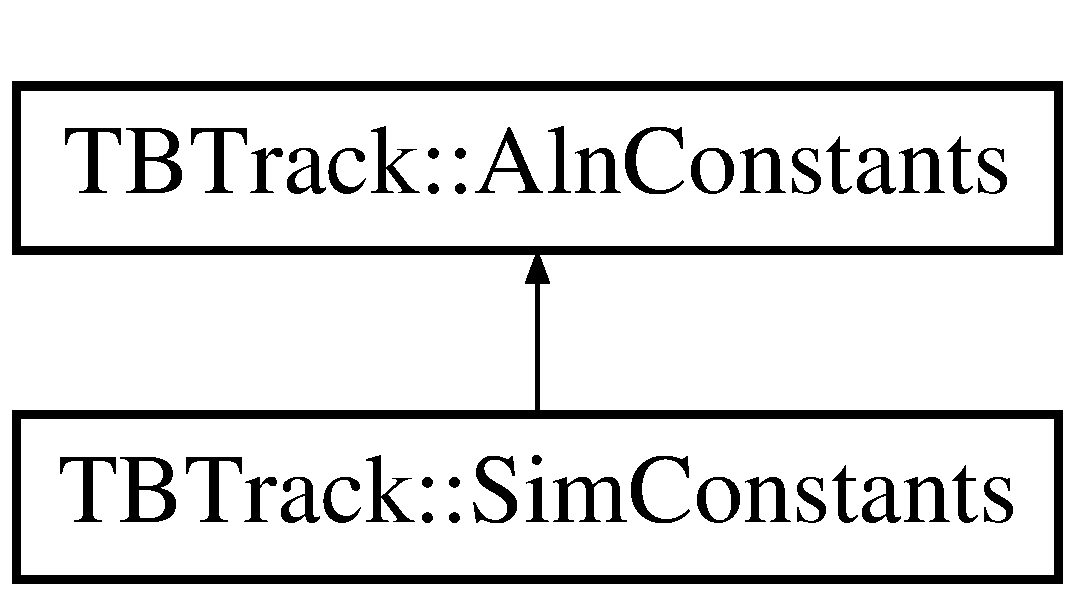
\includegraphics[height=2cm]{classTBTrack_1_1AlnConstants}
\end{center}
\end{figure}
\subsection*{Public Types}
\begin{DoxyCompactItemize}
\item 
enum \{ {\bfseries numberOfInts} = 0
 \}
\item 
enum \{ {\bfseries numberOfFloats} = 0
 \}
\item 
enum \{ {\bfseries numberOfDoubles} = 1+3$\ast$2$\ast$4
 \}
\end{DoxyCompactItemize}
\subsection*{Public Member Functions}
\begin{DoxyCompactItemize}
\item 
{\bfseries AlnConstants} (int period=0, int dataType=2)\label{classTBTrack_1_1AlnConstants_af91893338898d5c5d60add694f7ad53c}

\item 
double {\bfseries tdcUnit} () const \label{classTBTrack_1_1AlnConstants_af8ecb4ff47971cea86ea57719657405d}

\item 
void {\bfseries tdcUnit} (double t)\label{classTBTrack_1_1AlnConstants_a1070adc84db54a491c8ead531aa74bfe}

\item 
double {\bfseries cTzero} (unsigned d, unsigned l) const \label{classTBTrack_1_1AlnConstants_a92e168a711778633d7629411f6567ec6}

\item 
void {\bfseries cTzero} (unsigned d, unsigned l, double c)\label{classTBTrack_1_1AlnConstants_a02360b72db926a833aa6883221bb25c1}

\item 
double {\bfseries vDrift} (unsigned d, unsigned l) const \label{classTBTrack_1_1AlnConstants_a3e0815db478c533f423c090090ac7f58}

\item 
void {\bfseries vDrift} (unsigned d, unsigned l, double v)\label{classTBTrack_1_1AlnConstants_ab1801a04e89c0d92726ebaf82da6c7ea}

\item 
double {\bfseries vDquad} (unsigned d, unsigned l) const \label{classTBTrack_1_1AlnConstants_a502d35c057f8703828a8c4772c981372}

\item 
void {\bfseries vDquad} (unsigned d, unsigned l, double q)\label{classTBTrack_1_1AlnConstants_a69529ea7d72f1d98029aa479ef5f94a6}

\item 
double {\bfseries coordinate} (unsigned d, unsigned l, int t) const \label{classTBTrack_1_1AlnConstants_a4248f4f0634ada340af67a1e5129c5dc}

\item 
int {\bfseries tdcValue} (unsigned d, unsigned l, double c, double t=0.0) const \label{classTBTrack_1_1AlnConstants_aa51d47ab24355ca238e1e79ff8acf053}

\item 
std::ostream \& {\bfseries print} (std::ostream \&o=std::cout, const std::string \&s=\char`\"{}\char`\"{}) const \label{classTBTrack_1_1AlnConstants_aa01bb46450b492761c90392eb81411bc}

\item 
const int $\ast$ {\bfseries intData} () const \label{classTBTrack_1_1AlnConstants_afb793481bc8c9ea4786e9e52144cb708}

\item 
int $\ast$ {\bfseries intData} ()\label{classTBTrack_1_1AlnConstants_a5ffc45d080fe15974fca534ae01c3146}

\item 
const float $\ast$ {\bfseries floatData} () const \label{classTBTrack_1_1AlnConstants_a2d50c758aa6c1a6bbfa4790d7c1d1ed1}

\item 
float $\ast$ {\bfseries floatData} ()\label{classTBTrack_1_1AlnConstants_a48b746d9e7043bd80d2968bed18f21ef}

\item 
const double $\ast$ {\bfseries doubleData} () const \label{classTBTrack_1_1AlnConstants_afd83d2588465d22b8ef17cb39326ee5b}

\item 
double $\ast$ {\bfseries doubleData} ()\label{classTBTrack_1_1AlnConstants_aa07f0bb0b3cdde7eb56afa7050e626d9}

\end{DoxyCompactItemize}
\subsection*{Protected Attributes}
\begin{DoxyCompactItemize}
\item 
double {\bfseries \_\-tdcUnit}\label{classTBTrack_1_1AlnConstants_a2cf1c1f9615a86de4d37f9a72ff0292b}

\item 
double {\bfseries \_\-cTzero} [2][4]\label{classTBTrack_1_1AlnConstants_af55cc6424803c2d11d027bcec1b64f82}

\item 
double {\bfseries \_\-vDrift} [2][4]\label{classTBTrack_1_1AlnConstants_a31dab51bbeacb52b53f8d1bc2cd2466a}

\item 
double {\bfseries \_\-vDquad} [2][4]\label{classTBTrack_1_1AlnConstants_a91b9a4fcb791b1a3aeade9408633bbcf}

\end{DoxyCompactItemize}


\subsection{Detailed Description}


Definition at line 16 of file AlnConstants.hh.

The documentation for this class was generated from the following files:\begin{DoxyCompactItemize}
\item 
AlnConstants.hh\item 
AlnConstants.cc\end{DoxyCompactItemize}

\section{CALICE::AppendMultiAmplitude Class Reference}
\label{classCALICE_1_1AppendMultiAmplitude}\index{CALICE::AppendMultiAmplitude@{CALICE::AppendMultiAmplitude}}


Processor to add PAR\_\-MULTI\_\-AMPL (amplitude of the Multiplicity Counter) to the event.  


{\ttfamily \#include $<$AppendMultiAmplitude.hh$>$}\subsection*{Public Member Functions}
\begin{DoxyCompactItemize}
\item 
Processor $\ast$ {\bfseries newProcessor} ()\label{classCALICE_1_1AppendMultiAmplitude_af5c8a3fce4bc7612157e3d6ad50872d6}

\item 
void {\bfseries init} ()\label{classCALICE_1_1AppendMultiAmplitude_a528565bad5c83a2677bc752f4d47d1f6}

\item 
void {\bfseries processRunHeader} (LCRunHeader $\ast$run)\label{classCALICE_1_1AppendMultiAmplitude_a6c147a934e7b60ecbf788f7de33bfde9}

\item 
void {\bfseries processEvent} (LCEvent $\ast$evt)\label{classCALICE_1_1AppendMultiAmplitude_a80b214680c8275820126d7826b2ca0e0}

\item 
void {\bfseries end} ()\label{classCALICE_1_1AppendMultiAmplitude_a9976e1ce7c039db675881af775f68986}

\end{DoxyCompactItemize}
\subsection*{Protected Attributes}
\begin{DoxyCompactItemize}
\item 
std::string {\bfseries \_\-adcColName}\label{classCALICE_1_1AppendMultiAmplitude_a90acd521e292e3f2bdd9ff56b4606f55}

\item 
std::string {\bfseries \_\-connectionColName}\label{classCALICE_1_1AppendMultiAmplitude_a2902a95068d152cb11826aafe85f63bb}

\item 
std::string {\bfseries \_\-parNameMultiAmpl}\label{classCALICE_1_1AppendMultiAmplitude_a209412842c94a4ff6be9af6f7b41bf89}

\end{DoxyCompactItemize}
\subsection*{Private Member Functions}
\begin{DoxyCompactItemize}
\item 
void {\bfseries conditionsChanged} (lcio::LCCollection $\ast$col)\label{classCALICE_1_1AppendMultiAmplitude_ae04c6bc30a5a1bfc4700c2575ae09a76}

\end{DoxyCompactItemize}
\subsection*{Private Attributes}
\begin{DoxyCompactItemize}
\item 
unsigned int {\bfseries \_\-crate}\label{classCALICE_1_1AppendMultiAmplitude_a4ecf8796bb93026dbf2d680b7dd70214}

\item 
unsigned int {\bfseries \_\-slot}\label{classCALICE_1_1AppendMultiAmplitude_a281f76046ded3a3aa7c5880242caf1bd}

\item 
unsigned int {\bfseries \_\-fe}\label{classCALICE_1_1AppendMultiAmplitude_a0b02671cdf754fc52ab8fa6348293431}

\item 
unsigned int {\bfseries \_\-chip}\label{classCALICE_1_1AppendMultiAmplitude_aa15678d8ba0780fad8c59e546087781d}

\item 
unsigned int {\bfseries \_\-channel}\label{classCALICE_1_1AppendMultiAmplitude_ab205e6309046702fb743238a594a14fd}

\item 
bool {\bfseries \_\-connectionAvailable}\label{classCALICE_1_1AppendMultiAmplitude_af350bb41fd000d9968f9097cb91ad771}

\end{DoxyCompactItemize}


\subsection{Detailed Description}
Processor to add PAR\_\-MULTI\_\-AMPL (amplitude of the Multiplicity Counter) to the event. This processor adds an event parameter containing the amplitude of the analog multiplicity counter readout. The mapping of the multiplicity counter connection is read from the LCIO stream.

\begin{DoxyVersion}{Version}
1.0 
\end{DoxyVersion}
\begin{DoxyAuthor}{Author}
{\tt Benjamin.Lutz@desy.de} 

{\tt Nils.Feege@desy.de} 
\end{DoxyAuthor}
\begin{DoxyDate}{Date}
March 2010 
\end{DoxyDate}


Definition at line 25 of file AppendMultiAmplitude.hh.

The documentation for this class was generated from the following files:\begin{DoxyCompactItemize}
\item 
AppendMultiAmplitude.hh\item 
AppendMultiAmplitude.cc\end{DoxyCompactItemize}

\section{CALICE::AverageHistoryGraphs Class Reference}
\label{classCALICE_1_1AverageHistoryGraphs}\index{CALICE::AverageHistoryGraphs@{CALICE::AverageHistoryGraphs}}
Inheritance diagram for CALICE::AverageHistoryGraphs::\begin{figure}[H]
\begin{center}
\leavevmode
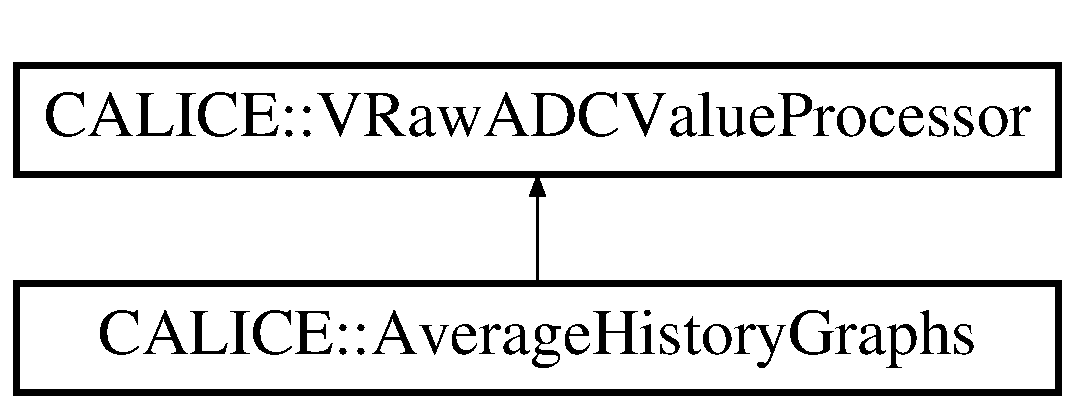
\includegraphics[height=2cm]{classCALICE_1_1AverageHistoryGraphs}
\end{center}
\end{figure}
\subsection*{Public Member Functions}
\begin{DoxyCompactItemize}
\item 
Processor $\ast$ {\bfseries newProcessor} ()\label{classCALICE_1_1AverageHistoryGraphs_aadeafdb3a9c7e2f355af43bbe2600a36}

\item 
void {\bf init} ()
\begin{DoxyCompactList}\small\item\em Called at the begin of the job before anything is read. \item\end{DoxyCompactList}\item 
void {\bf processRunHeader} (LCRunHeader $\ast$run)
\begin{DoxyCompactList}\small\item\em Called for every run, e.g. \item\end{DoxyCompactList}\item 
void {\bf processEvent} (LCEvent $\ast$evtP)
\begin{DoxyCompactList}\small\item\em Called for every event -\/ the working horse. \item\end{DoxyCompactList}\item 
void {\bfseries end} ()\label{classCALICE_1_1AverageHistoryGraphs_a66fdedb6f7f91bc59a2c5acb73d9e500}

\end{DoxyCompactItemize}
\subsection*{Protected Types}
\begin{DoxyCompactItemize}
\item 
enum {\bfseries EGraphType} \{ \par
{\bfseries kGraphMean}, 
{\bfseries kGraphRMS}, 
{\bfseries kGraphMin}, 
{\bfseries kGraphMax}, 
\par
{\bfseries kGraphWeight}, 
{\bfseries kNGraphTypes}
 \}
\item 
enum {\bfseries EHistoryType} \{ \par
{\bfseries kADCHistory}, 
{\bfseries kNoiseHistory}, 
{\bfseries kPedestalHistory}, 
{\bfseries kHitHistory}, 
\par
{\bfseries kNHistoryGraphs}
 \}
\item 
enum {\bfseries EStampType} \{ \par
{\bfseries kHistoryStamp}, 
{\bfseries kHistoryConfStamp}, 
{\bfseries kHistoryStateStamp}, 
{\bfseries kHistoryStateValue}, 
\par
{\bfseries kNHistoryStamps}
 \}
\end{DoxyCompactItemize}
\subsection*{Protected Member Functions}
\begin{DoxyCompactItemize}
\item 
void {\bfseries configurationChanged} (EVENT::LCCollection $\ast$)\label{classCALICE_1_1AverageHistoryGraphs_a176525151e7d59d850f171befa7d793b}

\item 
void {\bfseries moduleTypeChanged} (lcio::LCCollection $\ast$col)\label{classCALICE_1_1AverageHistoryGraphs_acdba66e246541547c5fb4ba032e4c781}

\item 
void {\bfseries moduleLocationChanged} (lcio::LCCollection $\ast$col)\label{classCALICE_1_1AverageHistoryGraphs_ab2da21acfb64312a3182becc51232998}

\item 
void {\bfseries moduleConnectionChanged} (lcio::LCCollection $\ast$col)\label{classCALICE_1_1AverageHistoryGraphs_a126a4d42d653c4c005a5135d0dfea159}

\item 
void {\bfseries resizeArrays} ()\label{classCALICE_1_1AverageHistoryGraphs_a1f1586ff5a3fe049d6613a296128bbcd}

\end{DoxyCompactItemize}
\subsection*{Protected Attributes}
\begin{DoxyCompactItemize}
\item 
Int\_\-t {\bfseries \_\-useTimeStamp}\label{classCALICE_1_1AverageHistoryGraphs_a924519564a5a56335cc071811de29594}

\item 
IntVec {\bfseries \_\-eventPar}\label{classCALICE_1_1AverageHistoryGraphs_a9cd19052bd65b4925f23feaa915086c3}

\item 
Int\_\-t {\bfseries \_\-avADCNMax}\label{classCALICE_1_1AverageHistoryGraphs_aaea631c4dde12b4da4274e9028b5bfa8}

\item 
Float\_\-t {\bfseries \_\-signalCut}\label{classCALICE_1_1AverageHistoryGraphs_abe695f79dbd74292894bc9e8b53a3324}

\item 
Int\_\-t {\bfseries \_\-skipCalibrationEventsAlways}\label{classCALICE_1_1AverageHistoryGraphs_a83a1b6b057c3e5c5b01aea6442864ed5}

\item 
std::string {\bfseries \_\-cellParameterCollectionName}\label{classCALICE_1_1AverageHistoryGraphs_a1eca22a5971a5a7d480ae8f9c14f74fb}

\item 
std::vector$<$ std::vector$<$ Average\_\-t $>$ $>$ {\bfseries \_\-avValues} [kNHistoryGraphs]\label{classCALICE_1_1AverageHistoryGraphs_ae0b1ef124d0704af661c3a6cff2c793a}

\item 
bool {\bfseries \_\-avADCIsValid}\label{classCALICE_1_1AverageHistoryGraphs_ac8f0ccd575282d74f9239f93e662faf7}

\item 
UInt\_\-t {\bfseries \_\-avADCn}\label{classCALICE_1_1AverageHistoryGraphs_adcdef8bfa777ecd9977e6e4c03b6177b}

\item 
std::vector$<$ std::vector$<$ Average\_\-t $>$ $>$ {\bfseries \_\-avADC}\label{classCALICE_1_1AverageHistoryGraphs_a09f9a1eb99e16951c1bb2219690d0332}

\item 
std::vector$<$ std::vector$<$ UInt\_\-t $>$ $>$ {\bfseries \_\-nHits}\label{classCALICE_1_1AverageHistoryGraphs_a9ac965b72b8eaf330366d65ca3e6bb40}

\item 
StringVec {\bfseries \_\-monitorConf}\label{classCALICE_1_1AverageHistoryGraphs_a98da6d927a6ed04dc03e91057181912c}

\item 
{\bf vector}$<$ ConditionsChangeDelegator$<$ {\bf AverageHistoryGraphs} $>$ $>$ {\bfseries \_\-confChanges}\label{classCALICE_1_1AverageHistoryGraphs_a03616ae3f8232db9aa14cbd67332cfe1}

\item 
bool {\bfseries \_\-confChanged}\label{classCALICE_1_1AverageHistoryGraphs_acd099e4c900efbc66f69f8cce8391f03}

\item 
UInt\_\-t {\bfseries \_\-nConfigurationChanges}\label{classCALICE_1_1AverageHistoryGraphs_aa18f88276066de50377761e7ce983cba}

\item 
Int\_\-t {\bfseries \_\-wasState}\label{classCALICE_1_1AverageHistoryGraphs_a8cc7262ec5a99b0562f812fd014a1c26}

\item 
UInt\_\-t {\bfseries \_\-nStateChanges}\label{classCALICE_1_1AverageHistoryGraphs_adbc2ad77c6f5945a98131e4af3cbd2ef}

\item 
{\bf histmgr::Key\_\-t} {\bfseries \_\-graphGroupKey}\label{classCALICE_1_1AverageHistoryGraphs_a5b92eb7bf713fc38bb4ab6a033477be6}

\item 
std::vector$<$ {\bf histmgr::Key\_\-t} $>$ {\bfseries \_\-avValueHistoryKey}\label{classCALICE_1_1AverageHistoryGraphs_a9b71e2d36930c41347fe49a0e8495b7d}

\item 
{\bf histmgr::Key\_\-t} {\bfseries \_\-stateChangeHistoryKey}\label{classCALICE_1_1AverageHistoryGraphs_a1f003a748d898ea24d416211dd8b9168}

\item 
{\bf histmgr::Key\_\-t} {\bfseries \_\-confChangeHistoryKey}\label{classCALICE_1_1AverageHistoryGraphs_af654242bdda2b428ba576813b6d46559}

\end{DoxyCompactItemize}
\subsection*{Static Protected Attributes}
\begin{DoxyCompactItemize}
\item 
static const char $\ast$ {\bfseries \_\-\_\-graphTypeNames} [kNGraphTypes]
\item 
static const char $\ast$ {\bfseries \_\-\_\-historyGraphNames} [kNHistoryGraphs]
\item 
static UInt\_\-t {\bfseries \_\-\_\-nSamplesPerChip} = 18\label{classCALICE_1_1AverageHistoryGraphs_a38373d247acaed96390b500046c523ac}

\item 
static UInt\_\-t {\bfseries \_\-\_\-nChips} = 12\label{classCALICE_1_1AverageHistoryGraphs_a376afe7cdb43b7a1ed6be6cdcfbc9bb5}

\end{DoxyCompactItemize}


\subsection{Detailed Description}


Definition at line 17 of file AverageHistoryGraphs.hh.

\subsection{Member Function Documentation}
\index{CALICE::AverageHistoryGraphs@{CALICE::AverageHistoryGraphs}!init@{init}}
\index{init@{init}!CALICE::AverageHistoryGraphs@{CALICE::AverageHistoryGraphs}}
\subsubsection[{init}]{\setlength{\rightskip}{0pt plus 5cm}void CALICE::AverageHistoryGraphs::init ()}\label{classCALICE_1_1AverageHistoryGraphs_a3734a824ecbe14585605e459c40b7f67}


Called at the begin of the job before anything is read. Use to initialize the processor, e.g. book histograms. 

Reimplemented from {\bf CALICE::VRawADCValueProcessor} \doxyref{}{p.}{classCALICE_1_1VRawADCValueProcessor}.

Definition at line 121 of file AverageHistoryGraphs.cc.

References histmgr::HistMgr::createGraphCollection(), histmgr::HistMgr::createHistogramGroup(), and histmgr::HistMgr::lockGroup().\index{CALICE::AverageHistoryGraphs@{CALICE::AverageHistoryGraphs}!processEvent@{processEvent}}
\index{processEvent@{processEvent}!CALICE::AverageHistoryGraphs@{CALICE::AverageHistoryGraphs}}
\subsubsection[{processEvent}]{\setlength{\rightskip}{0pt plus 5cm}void CALICE::AverageHistoryGraphs::processEvent (LCEvent $\ast$ {\em evtP})}\label{classCALICE_1_1AverageHistoryGraphs_a1b70e2c0f46158aac6fe28edb2ca23cf}


Called for every event -\/ the working horse. 

Definition at line 251 of file AverageHistoryGraphs.cc.

References CALICE::VRawADCValueProcessor::\_\-adcColName, histmgr::GraphCollection\_\-t::appendXValue(), histmgr::HistMgr::getGraphCollection(), CALICE::CellParameter::getNoise(), CALICE::CellParameter::getPedestal(), and histmgr::GraphCollection\_\-t::setYValue().\index{CALICE::AverageHistoryGraphs@{CALICE::AverageHistoryGraphs}!processRunHeader@{processRunHeader}}
\index{processRunHeader@{processRunHeader}!CALICE::AverageHistoryGraphs@{CALICE::AverageHistoryGraphs}}
\subsubsection[{processRunHeader}]{\setlength{\rightskip}{0pt plus 5cm}void CALICE::AverageHistoryGraphs::processRunHeader (LCRunHeader $\ast$ {\em run})\hspace{0.3cm}{\ttfamily  [inline]}}\label{classCALICE_1_1AverageHistoryGraphs_a0b55ddfdfa8bac7bc5f17cd94c695da6}


Called for every run, e.g. overwrite to initialize run dependent histograms. 

Definition at line 34 of file AverageHistoryGraphs.hh.

\subsection{Field Documentation}
\index{CALICE::AverageHistoryGraphs@{CALICE::AverageHistoryGraphs}!\_\-\_\-graphTypeNames@{\_\-\_\-graphTypeNames}}
\index{\_\-\_\-graphTypeNames@{\_\-\_\-graphTypeNames}!CALICE::AverageHistoryGraphs@{CALICE::AverageHistoryGraphs}}
\subsubsection[{\_\-\_\-graphTypeNames}]{\setlength{\rightskip}{0pt plus 5cm}const char $\ast$ CALICE::AverageHistoryGraphs::\_\-\_\-graphTypeNames\hspace{0.3cm}{\ttfamily  [static, protected]}}\label{classCALICE_1_1AverageHistoryGraphs_adce732f8a36e6b716ab80ff035b2603a}
{\bfseries Initial value:}
\begin{DoxyCode}
{
    "mean",
    "rms",
    "min",
    "max",
    "weight"
  }
\end{DoxyCode}


Definition at line 61 of file AverageHistoryGraphs.hh.\index{CALICE::AverageHistoryGraphs@{CALICE::AverageHistoryGraphs}!\_\-\_\-historyGraphNames@{\_\-\_\-historyGraphNames}}
\index{\_\-\_\-historyGraphNames@{\_\-\_\-historyGraphNames}!CALICE::AverageHistoryGraphs@{CALICE::AverageHistoryGraphs}}
\subsubsection[{\_\-\_\-historyGraphNames}]{\setlength{\rightskip}{0pt plus 5cm}const char $\ast$ CALICE::AverageHistoryGraphs::\_\-\_\-historyGraphNames\hspace{0.3cm}{\ttfamily  [static, protected]}}\label{classCALICE_1_1AverageHistoryGraphs_a2349f46d366705d3d312fbc32febf896}
{\bfseries Initial value:}
\begin{DoxyCode}
{
    "ADCHistory",
    "NoiseHistory",
    "PedestalHistory",
    "HitHistory"
  }
\end{DoxyCode}


Definition at line 62 of file AverageHistoryGraphs.hh.

The documentation for this class was generated from the following files:\begin{DoxyCompactItemize}
\item 
AverageHistoryGraphs.hh\item 
AverageHistoryGraphs.cc\end{DoxyCompactItemize}

\section{CALICE::BaseMappingIIProcessor Class Reference}
\label{classCALICE_1_1BaseMappingIIProcessor}\index{CALICE::BaseMappingIIProcessor@{CALICE::BaseMappingIIProcessor}}
Inheritance diagram for CALICE::BaseMappingIIProcessor::\begin{figure}[H]
\begin{center}
\leavevmode
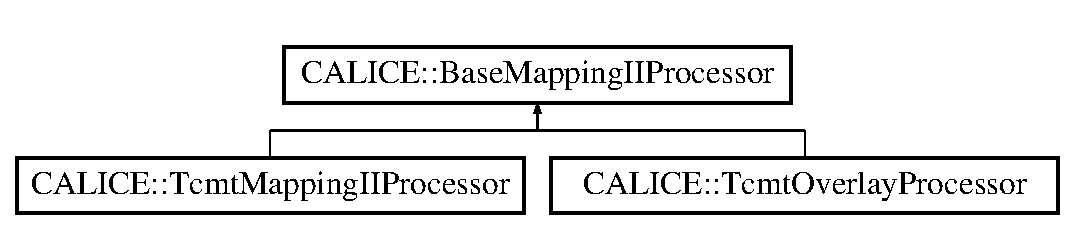
\includegraphics[height=2cm]{classCALICE_1_1BaseMappingIIProcessor}
\end{center}
\end{figure}
\subsection*{Public Member Functions}
\begin{DoxyCompactItemize}
\item 
{\bfseries BaseMappingIIProcessor} (const std::string \&typeName)\label{classCALICE_1_1BaseMappingIIProcessor_a8fe56d91380e26a12371e14a323d25d6}

\item 
virtual void {\bfseries init} ()\label{classCALICE_1_1BaseMappingIIProcessor_abb1ef572435bcc64898506d8f4c96cd9}

\item 
virtual void {\bfseries processRunHeader} (LCRunHeader $\ast$run)\label{classCALICE_1_1BaseMappingIIProcessor_a995afff29900be06e93ebe0453ed4aa6}

\item 
virtual void {\bfseries processEvent} (LCEvent $\ast$evt)=0\label{classCALICE_1_1BaseMappingIIProcessor_a5ac01e2e7f361f7ec4e1bd039ccbd33b}

\item 
virtual void {\bfseries check} (LCEvent $\ast$evt)\label{classCALICE_1_1BaseMappingIIProcessor_a4abb713a96256ee6599e9737e54bdfe1}

\item 
virtual void {\bfseries end} ()\label{classCALICE_1_1BaseMappingIIProcessor_a201450aeeedac3600901e6fd1d25ada6}

\end{DoxyCompactItemize}
\subsection*{Protected Member Functions}
\begin{DoxyCompactItemize}
\item 
virtual void {\bfseries updateInverseMap} ()\label{classCALICE_1_1BaseMappingIIProcessor_a60b39bae8ec80110e15b126c77138103}

\item 
virtual void {\bfseries moduleTypeChanged} (lcio::LCCollection $\ast$col)\label{classCALICE_1_1BaseMappingIIProcessor_a016f786152f13a2dbb7a0ca9c0727a08}

\item 
virtual void {\bfseries moduleLocationChanged} (lcio::LCCollection $\ast$col)\label{classCALICE_1_1BaseMappingIIProcessor_a9b65e70f55abef48ee724dab92c2b5db}

\item 
virtual void {\bfseries moduleConnectionChanged} (lcio::LCCollection $\ast$col)\label{classCALICE_1_1BaseMappingIIProcessor_a4ea22fa131cd52bdb59a9dc0d49bb033}

\item 
virtual void {\bfseries detectorTransformationChanged} (lcio::LCCollection $\ast$col)\label{classCALICE_1_1BaseMappingIIProcessor_ac82c048d8b7e3f28fe3b17b4855bb989}

\item 
virtual void {\bfseries referenceTransformationChanged} (lcio::LCCollection $\ast$col)\label{classCALICE_1_1BaseMappingIIProcessor_a5e17c0ecedbbb704f21f94091aeb61f0}

\end{DoxyCompactItemize}
\subsection*{Protected Attributes}
\begin{DoxyCompactItemize}
\item 
std::string {\bfseries \_\-inputColName}\label{classCALICE_1_1BaseMappingIIProcessor_a89f87c70722b470ce3351a1a94a04c5d}

\item 
std::string {\bfseries \_\-outputColName}\label{classCALICE_1_1BaseMappingIIProcessor_a55c4612d6057c09ccabb5bce43cfd184}

\item 
std::string {\bfseries \_\-colNameModuleDescription}\label{classCALICE_1_1BaseMappingIIProcessor_a3cf654ae79db0b075343f05f66b86974}

\item 
std::string {\bfseries \_\-colNameModuleLocation}\label{classCALICE_1_1BaseMappingIIProcessor_a2ca5ef0fe54cf330a00b5a89fe7baacf}

\item 
std::string {\bfseries \_\-colNameModuleConnection}\label{classCALICE_1_1BaseMappingIIProcessor_a0a03a8f94ec07d56db8cb88174fe72cd}

\item 
std::string {\bfseries \_\-colNameDetectorTransformation}\label{classCALICE_1_1BaseMappingIIProcessor_aed612620eab1d8ebeb5a584826f70781}

\item 
std::string {\bfseries \_\-colNameReferenceTransformation}\label{classCALICE_1_1BaseMappingIIProcessor_a944b28e0d8de4b183e9dced0d24aa863}

\item 
ConditionsChangeDelegator$<$ {\bf BaseMappingIIProcessor} $>$ {\bfseries \_\-moduleTypeChange}\label{classCALICE_1_1BaseMappingIIProcessor_aec48652f1896782024ba9cf85eaeb0f9}

\item 
ConditionsChangeDelegator$<$ {\bf BaseMappingIIProcessor} $>$ {\bfseries \_\-moduleLocationChange}\label{classCALICE_1_1BaseMappingIIProcessor_abbc58227157b9c1c293845f46e41b37a}

\item 
ConditionsChangeDelegator$<$ {\bf BaseMappingIIProcessor} $>$ {\bfseries \_\-moduleConnectionChange}\label{classCALICE_1_1BaseMappingIIProcessor_a862d6f636084c8a5b97a3d325aaf9115}

\item 
ConditionsChangeDelegator$<$ {\bf BaseMappingIIProcessor} $>$ {\bfseries \_\-detectorTransformationChange}\label{classCALICE_1_1BaseMappingIIProcessor_abd2368662503bb079b2e60e10c5ff77f}

\item 
ConditionsChangeDelegator$<$ {\bf BaseMappingIIProcessor} $>$ {\bfseries \_\-referenceTransformationChange}\label{classCALICE_1_1BaseMappingIIProcessor_a265f357118f9770bf12edf8c4144338f}

\item 
MappingAndAlignment {\bfseries \_\-mapping}\label{classCALICE_1_1BaseMappingIIProcessor_a41bfff962f24cc68687dcf4b482db560}

\item 
bool {\bfseries \_\-viewConnectionTree}\label{classCALICE_1_1BaseMappingIIProcessor_ae06d06bfae0591fb5f89b749f476af13}

\item 
std::map$<$ unsigned, unsigned $>$ {\bfseries \_\-inverseModuleMap}\label{classCALICE_1_1BaseMappingIIProcessor_aa4baf288fa623c98ec56a5c97e2b6b08}

\end{DoxyCompactItemize}


\subsection{Detailed Description}


Definition at line 31 of file BaseMappingIIProcessor.hh.

The documentation for this class was generated from the following files:\begin{DoxyCompactItemize}
\item 
BaseMappingIIProcessor.hh\item 
BaseMappingIIProcessor.cc\end{DoxyCompactItemize}

\section{CALICE::Box Class Reference}
\label{classCALICE_1_1Box}\index{CALICE::Box@{CALICE::Box}}


Helper class to calculate an envelop cuboid around hit collections.  


{\ttfamily \#include $<$Box.hh$>$}\subsection*{Public Member Functions}
\begin{DoxyCompactItemize}
\item 
void {\bf reset} ()\label{classCALICE_1_1Box_ab3f1dc40177112886cf159f568efa6d7}

\begin{DoxyCompactList}\small\item\em Remove all hits from the box. \item\end{DoxyCompactList}\item 
void {\bf add} (const EVENT::CalorimeterHit $\ast$a\_\-hit)
\begin{DoxyCompactList}\small\item\em Add a new hit to the box. \item\end{DoxyCompactList}\item 
void {\bf add} (const {\bf Box} \&a)
\begin{DoxyCompactList}\small\item\em Add all hits from the given box and recalculate the envelop. \item\end{DoxyCompactList}\item 
Bool\_\-t {\bf closerToEnvelopThan} (Float\_\-t distance, const {\bf ThreeVector\_\-t} $\ast$a) const \label{classCALICE_1_1Box_a7aaf4c49b26f3a3840eb24679247367b}

\begin{DoxyCompactList}\small\item\em Return true if the given position is closer to the envelop than the specified distance. \item\end{DoxyCompactList}\item 
Bool\_\-t {\bf closerToEnvelopThan} (Float\_\-t distance, const {\bf Box} \&a\_\-cluster) const \label{classCALICE_1_1Box_a99e38c13ebdb9aeabad211ac3911d234}

\begin{DoxyCompactList}\small\item\em Return true if the given box is closer to this box than the specified distance. \item\end{DoxyCompactList}\item 
Double\_\-t {\bf minDistanceToPoints} (const EVENT::CalorimeterHit $\ast$a\_\-hit) const \label{classCALICE_1_1Box_af4a9209ec249071bb52fdd40ef6a194c}

\begin{DoxyCompactList}\small\item\em Return the minimum distance of the given hits from the hits contained in this box. \item\end{DoxyCompactList}\item 
Double\_\-t {\bf minDistanceToPoints} (const {\bf ThreeVector\_\-t} $\ast$hit\_\-point) const \label{classCALICE_1_1Box_a2479a14154dddc489776721efd5f036d}

\begin{DoxyCompactList}\small\item\em Return the minimum distance of the given position from the hits contained in this box. \item\end{DoxyCompactList}\item 
void {\bf show} ()\label{classCALICE_1_1Box_a87a483695664352615623730f05fd441}

\begin{DoxyCompactList}\small\item\em Print out the positiosn of all contained hits. \item\end{DoxyCompactList}\item 
void {\bf calculateSize} ()\label{classCALICE_1_1Box_aa4bac160c1d2eadeb5f7e61ddec4f664}

\begin{DoxyCompactList}\small\item\em Calculate the envelop. \item\end{DoxyCompactList}\item 
Double\_\-t {\bf getSize} (UInt\_\-t i) const 
\begin{DoxyCompactList}\small\item\em Get the dimensions of one axis. \item\end{DoxyCompactList}\item 
Bool\_\-t {\bf isMerged} () const 
\begin{DoxyCompactList}\small\item\em Return true if this box was merged with another one. \item\end{DoxyCompactList}\item 
void {\bf setMerged} ()\label{classCALICE_1_1Box_a263ee0e337921d5ddd2090bfa7b69713}

\begin{DoxyCompactList}\small\item\em Set the status to \char`\"{}merged\char`\"{}. \item\end{DoxyCompactList}\end{DoxyCompactItemize}
\subsection*{Data Fields}
\begin{DoxyCompactItemize}
\item 
{\bf ThreeVector\_\-t} {\bfseries \_\-low}\label{classCALICE_1_1Box_adbb71adc36a978ff83b6c3ebb21c9705}

\item 
{\bf ThreeVector\_\-t} {\bfseries \_\-high}\label{classCALICE_1_1Box_a1146f0bc27c7e6beb495cf697ef9d0b1}

\item 
std::vector$<$ const EVENT::CalorimeterHit $\ast$ $>$ {\bf \_\-hits}
\begin{DoxyCompactList}\small\item\em the hit collection contained in this box. \item\end{DoxyCompactList}\item 
{\bf Stat\_\-t} {\bf \_\-mean} [3]
\begin{DoxyCompactList}\small\item\em the position of the box centre and its dimesnion (all three axis). \item\end{DoxyCompactList}\item 
Bool\_\-t {\bf \_\-merged}
\begin{DoxyCompactList}\small\item\em true if this box is merged with another one. \item\end{DoxyCompactList}\end{DoxyCompactItemize}


\subsection{Detailed Description}
Helper class to calculate an envelop cuboid around hit collections. This class can be used to quickly reject hits which are far away from the hit collection contained in this box. 

Definition at line 42 of file Box.hh.

\subsection{Member Function Documentation}
\index{CALICE::Box@{CALICE::Box}!add@{add}}
\index{add@{add}!CALICE::Box@{CALICE::Box}}
\subsubsection[{add}]{\setlength{\rightskip}{0pt plus 5cm}void CALICE::Box::add (const {\bf Box} \& {\em a})\hspace{0.3cm}{\ttfamily  [inline]}}\label{classCALICE_1_1Box_af8071d168d578b5c4046ed25da089d4c}


Add all hits from the given box and recalculate the envelop. The envelop is not calculated automatically. \begin{DoxySeeAlso}{See also}
\doxyref{calculateSize}{p.}{classCALICE_1_1Box_aa4bac160c1d2eadeb5f7e61ddec4f664}. 
\end{DoxySeeAlso}


Definition at line 77 of file Box.hh.

References \_\-hits, and add().\index{CALICE::Box@{CALICE::Box}!add@{add}}
\index{add@{add}!CALICE::Box@{CALICE::Box}}
\subsubsection[{add}]{\setlength{\rightskip}{0pt plus 5cm}void CALICE::Box::add (const EVENT::CalorimeterHit $\ast$ {\em a\_\-hit})\hspace{0.3cm}{\ttfamily  [inline]}}\label{classCALICE_1_1Box_ad1fbc523839d5544ac0def273f3b6042}


Add a new hit to the box. The envelop is not calculated automatically. \begin{DoxySeeAlso}{See also}
\doxyref{calculateSize}{p.}{classCALICE_1_1Box_aa4bac160c1d2eadeb5f7e61ddec4f664}. 
\end{DoxySeeAlso}


Definition at line 55 of file Box.hh.

References \_\-hits, and \_\-mean.

Referenced by add().\index{CALICE::Box@{CALICE::Box}!getSize@{getSize}}
\index{getSize@{getSize}!CALICE::Box@{CALICE::Box}}
\subsubsection[{getSize}]{\setlength{\rightskip}{0pt plus 5cm}Double\_\-t CALICE::Box::getSize (UInt\_\-t {\em i}) const\hspace{0.3cm}{\ttfamily  [inline]}}\label{classCALICE_1_1Box_a8c499525edb4c0ea185df58b2a0a89d3}


Get the dimensions of one axis. 
\begin{DoxyParams}{Parameters}
\item[{\em i}]axis (0-\/2). \end{DoxyParams}


Definition at line 173 of file Box.hh.

References \_\-mean.\index{CALICE::Box@{CALICE::Box}!isMerged@{isMerged}}
\index{isMerged@{isMerged}!CALICE::Box@{CALICE::Box}}
\subsubsection[{isMerged}]{\setlength{\rightskip}{0pt plus 5cm}Bool\_\-t CALICE::Box::isMerged () const\hspace{0.3cm}{\ttfamily  [inline]}}\label{classCALICE_1_1Box_a5ae481b0b52563ce15dc6e8312e729b3}


Return true if this box was merged with another one. If a box is merged all hits are added to the box with which it is merged. Thus, the same hits are stored in two boxes. 

Definition at line 179 of file Box.hh.

References \_\-merged.

\subsection{Field Documentation}
\index{CALICE::Box@{CALICE::Box}!\_\-hits@{\_\-hits}}
\index{\_\-hits@{\_\-hits}!CALICE::Box@{CALICE::Box}}
\subsubsection[{\_\-hits}]{\setlength{\rightskip}{0pt plus 5cm}std::vector$<$const EVENT::CalorimeterHit$\ast$$>$ {\bf CALICE::Box::\_\-hits}}\label{classCALICE_1_1Box_a59a8242b3a5b00a253a997fe3e2c977a}


the hit collection contained in this box. 

Definition at line 188 of file Box.hh.

Referenced by add(), minDistanceToPoints(), reset(), and show().\index{CALICE::Box@{CALICE::Box}!\_\-mean@{\_\-mean}}
\index{\_\-mean@{\_\-mean}!CALICE::Box@{CALICE::Box}}
\subsubsection[{\_\-mean}]{\setlength{\rightskip}{0pt plus 5cm}{\bf Stat\_\-t} {\bf CALICE::Box::\_\-mean}[3]}\label{classCALICE_1_1Box_ae964c5ea0f130bc42b090d82cd909ee8}


the position of the box centre and its dimesnion (all three axis). 

Definition at line 189 of file Box.hh.

Referenced by add(), calculateSize(), getSize(), reset(), and show().\index{CALICE::Box@{CALICE::Box}!\_\-merged@{\_\-merged}}
\index{\_\-merged@{\_\-merged}!CALICE::Box@{CALICE::Box}}
\subsubsection[{\_\-merged}]{\setlength{\rightskip}{0pt plus 5cm}Bool\_\-t {\bf CALICE::Box::\_\-merged}}\label{classCALICE_1_1Box_a746e0bdaa3f3039bf02d81e045659963}


true if this box is merged with another one. 

Definition at line 190 of file Box.hh.

Referenced by isMerged(), reset(), and setMerged().

The documentation for this class was generated from the following file:\begin{DoxyCompactItemize}
\item 
Box.hh\end{DoxyCompactItemize}

\section{CALICE::CalibrateAndApplyThreshold Class Reference}
\label{classCALICE_1_1CalibrateAndApplyThreshold}\index{CALICE::CalibrateAndApplyThreshold@{CALICE::CalibrateAndApplyThreshold}}


Marlin Processor to go from RawCalorimeterHit to calibrated CalorimeterHits.  


{\ttfamily \#include $<$CalibrateAndApplyThreshold.hh$>$}Inheritance diagram for CALICE::CalibrateAndApplyThreshold::\begin{figure}[H]
\begin{center}
\leavevmode
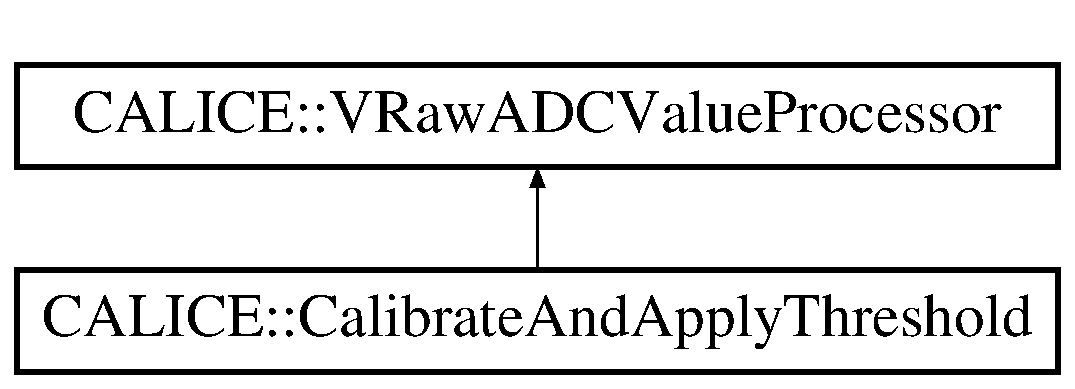
\includegraphics[height=2cm]{classCALICE_1_1CalibrateAndApplyThreshold}
\end{center}
\end{figure}
\subsection*{Public Member Functions}
\begin{DoxyCompactItemize}
\item 
Processor $\ast$ {\bf newProcessor} ()\label{classCALICE_1_1CalibrateAndApplyThreshold_a011ca53f853d3a6bc58d1a9a541a99da}

\begin{DoxyCompactList}\small\item\em construct a new Processor (required by Marlin). \item\end{DoxyCompactList}\item 
{\bf CalibrateAndApplyThreshold} ()
\begin{DoxyCompactList}\small\item\em default constructor. \item\end{DoxyCompactList}\item 
{\bf $\sim$CalibrateAndApplyThreshold} ()\label{classCALICE_1_1CalibrateAndApplyThreshold_a1318d9f3f1a695b1996c30c63c47d085}

\begin{DoxyCompactList}\small\item\em destructor. \item\end{DoxyCompactList}\item 
void {\bf init} ()
\begin{DoxyCompactList}\small\item\em Called at the begin of the job before anything is read. \item\end{DoxyCompactList}\item 
void {\bf processRunHeader} (LCRunHeader $\ast$run)
\begin{DoxyCompactList}\small\item\em Called for every run (does nothing. \item\end{DoxyCompactList}\item 
void {\bf processEvent} (LCEvent $\ast$evtP)
\begin{DoxyCompactList}\small\item\em Reconstruct calorimeter hits. \item\end{DoxyCompactList}\item 
void {\bfseries end} ()\label{classCALICE_1_1CalibrateAndApplyThreshold_a9779b4e112b4cae16dec00d158f656f2}

\end{DoxyCompactItemize}
\subsection*{Private Member Functions}
\begin{DoxyCompactItemize}
\item 
void {\bfseries detectorTransformationChanged} (lcio::LCCollection $\ast$col)\label{classCALICE_1_1CalibrateAndApplyThreshold_a160acdea77969ab85d10dfbf4ba6b719}

\item 
void {\bfseries referenceTransformationChanged} (lcio::LCCollection $\ast$col)\label{classCALICE_1_1CalibrateAndApplyThreshold_aca4443deb520f3c16061d3d2364ccf16}

\end{DoxyCompactItemize}
\subsection*{Private Attributes}
\begin{DoxyCompactItemize}
\item 
{\bf Calibration} $\ast$ {\bfseries \_\-calibration}\label{classCALICE_1_1CalibrateAndApplyThreshold_a5f7e659b256a90f073328936dfca032d}

\item 
LCCollection $\ast$ {\bfseries \_\-cellCol}\label{classCALICE_1_1CalibrateAndApplyThreshold_a1379ee3029e35c09bcf02a555f79bce2}

\item 
std::string {\bfseries \_\-cellParameterCollectionName}\label{classCALICE_1_1CalibrateAndApplyThreshold_aaee3b361269a3d245228c6a7b0866f0e}

\item 
IntVec {\bfseries \_\-adcRange}\label{classCALICE_1_1CalibrateAndApplyThreshold_a930eaf481f0ed35420ee5a4c87e50bc5}

\item 
Float\_\-t {\bf \_\-signalThreshold}
\begin{DoxyCompactList}\small\item\em Signals above the signal threshold and . \item\end{DoxyCompactList}\item 
FloatVec {\bf \_\-noiseCutVec}
\begin{DoxyCompactList}\small\item\em above the noise cut are considered to be hits. \item\end{DoxyCompactList}\item 
Float\_\-t {\bf \_\-noiseCut}\label{classCALICE_1_1CalibrateAndApplyThreshold_a457ab672e3467ed409a58e42e4aa6229}

\begin{DoxyCompactList}\small\item\em will be set by the first element of the \_\-noiseCutVec \item\end{DoxyCompactList}\item 
std::string {\bf \_\-rawhitColName}
\begin{DoxyCompactList}\small\item\em Name of the hit collection (INPUT). \item\end{DoxyCompactList}\item 
std::string {\bf \_\-hitColName}
\begin{DoxyCompactList}\small\item\em Name of the hit collection (OUTPUT). \item\end{DoxyCompactList}\item 
bool {\bf \_\-linkRecToSim}\label{classCALICE_1_1CalibrateAndApplyThreshold_aba8a11b61c43b9339e3140839fc5b213}

\begin{DoxyCompactList}\small\item\em kkk flag to disable/enable the creation of an LCRelation to simulated hit \item\end{DoxyCompactList}\item 
std::string {\bf \_\-RecToSimColName}
\begin{DoxyCompactList}\small\item\em kkk: Name of the relation collection hit -\/$>$ simhit (OUTPUT). \item\end{DoxyCompactList}\item 
std::string {\bf \_\-RawToSimColName}
\begin{DoxyCompactList}\small\item\em Name of the relation collection between Sim and Raw hits (INPUT). \item\end{DoxyCompactList}\item 
std::string {\bf \_\-calibrationObjectName}\label{classCALICE_1_1CalibrateAndApplyThreshold_a36efa661235242659c74a49235164662}

\begin{DoxyCompactList}\small\item\em Name of the \doxyref{Calibration}{p.}{classCalibration} object to be used (will be created using the \doxyref{CalibrationFactory}{p.}{classCalibrationFactory}). \item\end{DoxyCompactList}\item 
std::string {\bf \_\-calibrationConstantColName}
\begin{DoxyCompactList}\small\item\em Name of the conditions data collection containing the calibration constants. \item\end{DoxyCompactList}\item 
Bool\_\-t {\bfseries \_\-calibrationOn}\label{classCALICE_1_1CalibrateAndApplyThreshold_a1381fda668d89ec76ac565580e7fca36}

\item 
UInt\_\-t {\bfseries \_\-lastEvent}\label{classCALICE_1_1CalibrateAndApplyThreshold_ab2f19b2717ad2afc75043a35478f3ceb}

\item 
UInt\_\-t {\bfseries \_\-nEventsWithoutRAWHITS}\label{classCALICE_1_1CalibrateAndApplyThreshold_acf199915d32e1c4cb6d9a87f4a0373ff}

\item 
UInt\_\-t {\bfseries \_\-nEventsWithoutSIMHITS}\label{classCALICE_1_1CalibrateAndApplyThreshold_ae3e308ce27f5c1dd19bfee64a4d68892}

\item 
UInt\_\-t {\bfseries \_\-nEvt}\label{classCALICE_1_1CalibrateAndApplyThreshold_a80c7d9d42453384e5f8b12eee3e6b377}

\item 
Int\_\-t {\bfseries \_\-saveHistograms}\label{classCALICE_1_1CalibrateAndApplyThreshold_a05f90325598b42ff4e8b0af45cedc99b}

\item 
RunInformation {\bfseries \_\-runInfo}\label{classCALICE_1_1CalibrateAndApplyThreshold_afa4a2e593f7eabd44817705637f2f5b8}

\item 
TString {\bfseries \_\-rootname}\label{classCALICE_1_1CalibrateAndApplyThreshold_ad54aa68d7f9f558d3556c1e387043e0b}

\item 
TFile $\ast$ {\bfseries \_\-hfile}\label{classCALICE_1_1CalibrateAndApplyThreshold_adfab3548f6b0c6e4cce5436cc679bfb6}

\item 
TH1F $\ast$ {\bfseries p\_\-noise} [30][324]\label{classCALICE_1_1CalibrateAndApplyThreshold_a2a1569bd1101d3c46b178524e2280953}

\item 
TH1F $\ast$ {\bfseries p\_\-rawAmpl} [30][324]\label{classCALICE_1_1CalibrateAndApplyThreshold_a0773507c8f06882bb5c7b62fd4ac533b}

\item 
TH1F $\ast$ {\bfseries p\_\-pedCorr} [30][324]\label{classCALICE_1_1CalibrateAndApplyThreshold_ae1a721c77f3bf49fffff7ec31fddb214}

\item 
TH1F $\ast$ {\bfseries p\_\-calVal} [30][324]\label{classCALICE_1_1CalibrateAndApplyThreshold_ae443cba04fd5819e9a42cd514fb9ca50}

\item 
TH1F $\ast$ {\bfseries p\_\-sig} [30][324]\label{classCALICE_1_1CalibrateAndApplyThreshold_a479cc39be89fcaa154f96571e63843d4}

\item 
TH1F $\ast$ {\bfseries p\_\-SoN} [30][324]\label{classCALICE_1_1CalibrateAndApplyThreshold_a8d5fb256bddd8b8aad93138bbf50c1d7}

\item 
std::string {\bf \_\-colNameDetectorTransformation}
\begin{DoxyCompactList}\small\item\em Name of the conditions data collection which describes the position and the rotation of the detector. \item\end{DoxyCompactList}\item 
std::string {\bf \_\-colNameReferenceTransformation}
\begin{DoxyCompactList}\small\item\em Name of the conditions data collection which describes the reference position and rotation. \item\end{DoxyCompactList}\item 
ConditionsChangeDelegator$<$ {\bf CalibrateAndApplyThreshold} $>$ {\bf \_\-detectorTransformationChange}
\begin{DoxyCompactList}\small\item\em helper class to listen for changes of the detector position or rotation. \item\end{DoxyCompactList}\item 
ConditionsChangeDelegator$<$ {\bf CalibrateAndApplyThreshold} $>$ {\bf \_\-referenceTransformationChange}
\begin{DoxyCompactList}\small\item\em helper class to listen for changes of the reference position or rotation. \item\end{DoxyCompactList}\item 
float {\bfseries \_\-fallbackShift}\label{classCALICE_1_1CalibrateAndApplyThreshold_a23959025f1e0fb5c0a177cd6ebbaa217}

\end{DoxyCompactItemize}


\subsection{Detailed Description}
Marlin Processor to go from RawCalorimeterHit to calibrated CalorimeterHits. The hit position is calculated using information stored in a the cellID1. Moreover, the signal is calibrated if a proper calibration object exists. should run on Data as well as on MC after digisim. \begin{Desc}
\item[{\bf Todo}](Re-\/)Verify its applicability for MC after modifs for this release!!!! \end{Desc}


Definition at line 36 of file CalibrateAndApplyThreshold.hh.

\subsection{Constructor \& Destructor Documentation}
\index{CALICE::CalibrateAndApplyThreshold@{CALICE::CalibrateAndApplyThreshold}!CalibrateAndApplyThreshold@{CalibrateAndApplyThreshold}}
\index{CalibrateAndApplyThreshold@{CalibrateAndApplyThreshold}!CALICE::CalibrateAndApplyThreshold@{CALICE::CalibrateAndApplyThreshold}}
\subsubsection[{CalibrateAndApplyThreshold}]{\setlength{\rightskip}{0pt plus 5cm}CALICE::CalibrateAndApplyThreshold::CalibrateAndApplyThreshold ()}\label{classCALICE_1_1CalibrateAndApplyThreshold_ae2d615ca7797434d642f1ae6d6950974}


default constructor. defines and registers its parameters. 

Definition at line 46 of file CalibrateAndApplyThreshold.cc.

References \_\-calibrationConstantColName, \_\-calibrationObjectName, \_\-colNameDetectorTransformation, \_\-colNameReferenceTransformation, \_\-hitColName, \_\-linkRecToSim, \_\-noiseCutVec, \_\-rawhitColName, \_\-RawToSimColName, \_\-RecToSimColName, and \_\-signalThreshold.

\subsection{Member Function Documentation}
\index{CALICE::CalibrateAndApplyThreshold@{CALICE::CalibrateAndApplyThreshold}!init@{init}}
\index{init@{init}!CALICE::CalibrateAndApplyThreshold@{CALICE::CalibrateAndApplyThreshold}}
\subsubsection[{init}]{\setlength{\rightskip}{0pt plus 5cm}void CALICE::CalibrateAndApplyThreshold::init ()}\label{classCALICE_1_1CalibrateAndApplyThreshold_a69d43c0be2a238e99828c918003bde74}


Called at the begin of the job before anything is read. Use to initialize the processor, e.g. book histograms. 

Reimplemented from {\bf CALICE::VRawADCValueProcessor} \doxyref{}{p.}{classCALICE_1_1VRawADCValueProcessor}.

Definition at line 142 of file CalibrateAndApplyThreshold.cc.

References \_\-calibrationConstantColName, \_\-calibrationObjectName, \_\-colNameDetectorTransformation, CALICE::VRawADCValueProcessor::\_\-colNameModuleDescription, \_\-colNameReferenceTransformation, \_\-detectorTransformationChange, \_\-noiseCut, \_\-noiseCutVec, \_\-referenceTransformationChange, CalibrationFactory::createCalibrationObject(), CalibrationFactory::getInstance(), and CalibrationFactory::listKits().\index{CALICE::CalibrateAndApplyThreshold@{CALICE::CalibrateAndApplyThreshold}!processEvent@{processEvent}}
\index{processEvent@{processEvent}!CALICE::CalibrateAndApplyThreshold@{CALICE::CalibrateAndApplyThreshold}}
\subsubsection[{processEvent}]{\setlength{\rightskip}{0pt plus 5cm}void CALICE::CalibrateAndApplyThreshold::processEvent (LCEvent $\ast$ {\em evtP})}\label{classCALICE_1_1CalibrateAndApplyThreshold_a2c3e34db11fe08fab2b184cc87f4d7b5}


Reconstruct calorimeter hits. The class needs as input the RawCalorimeterHit collection from \doxyref{SimpleHitSearch}{p.}{classCALICE_1_1SimpleHitSearch} or digisim and produces a CalorimeterHit collection. 

Definition at line 247 of file CalibrateAndApplyThreshold.cc.

References \_\-hitColName, \_\-linkRecToSim, \_\-noiseCut, \_\-rawhitColName, \_\-RawToSimColName, \_\-RecToSimColName, \_\-signalThreshold, Calibration::getCalibratedValue(), Calibration::getMiniumADCForMipThreshold(), CALICE::NoiseParameter::getNoise(), and CALICE::NoiseParameter::isDead().\index{CALICE::CalibrateAndApplyThreshold@{CALICE::CalibrateAndApplyThreshold}!processRunHeader@{processRunHeader}}
\index{processRunHeader@{processRunHeader}!CALICE::CalibrateAndApplyThreshold@{CALICE::CalibrateAndApplyThreshold}}
\subsubsection[{processRunHeader}]{\setlength{\rightskip}{0pt plus 5cm}void CALICE::CalibrateAndApplyThreshold::processRunHeader (LCRunHeader $\ast$ {\em run})}\label{classCALICE_1_1CalibrateAndApplyThreshold_a3bd3d21d979363fa105e7cea54148502}


Called for every run (does nothing. ) 

Definition at line 217 of file CalibrateAndApplyThreshold.cc.

References Calibration::isValid().

\subsection{Field Documentation}
\index{CALICE::CalibrateAndApplyThreshold@{CALICE::CalibrateAndApplyThreshold}!\_\-calibrationConstantColName@{\_\-calibrationConstantColName}}
\index{\_\-calibrationConstantColName@{\_\-calibrationConstantColName}!CALICE::CalibrateAndApplyThreshold@{CALICE::CalibrateAndApplyThreshold}}
\subsubsection[{\_\-calibrationConstantColName}]{\setlength{\rightskip}{0pt plus 5cm}std::string {\bf CALICE::CalibrateAndApplyThreshold::\_\-calibrationConstantColName}\hspace{0.3cm}{\ttfamily  [private]}}\label{classCALICE_1_1CalibrateAndApplyThreshold_a79e5cf6fc879e14cdd3c68f88b1ff7c1}


Name of the conditions data collection containing the calibration constants. 

Definition at line 100 of file CalibrateAndApplyThreshold.hh.

Referenced by CalibrateAndApplyThreshold(), and init().\index{CALICE::CalibrateAndApplyThreshold@{CALICE::CalibrateAndApplyThreshold}!\_\-colNameDetectorTransformation@{\_\-colNameDetectorTransformation}}
\index{\_\-colNameDetectorTransformation@{\_\-colNameDetectorTransformation}!CALICE::CalibrateAndApplyThreshold@{CALICE::CalibrateAndApplyThreshold}}
\subsubsection[{\_\-colNameDetectorTransformation}]{\setlength{\rightskip}{0pt plus 5cm}std::string {\bf CALICE::CalibrateAndApplyThreshold::\_\-colNameDetectorTransformation}\hspace{0.3cm}{\ttfamily  [private]}}\label{classCALICE_1_1CalibrateAndApplyThreshold_a4a6e48e29b530ac9b80375776cd4af31}


Name of the conditions data collection which describes the position and the rotation of the detector. 

Definition at line 124 of file CalibrateAndApplyThreshold.hh.

Referenced by CalibrateAndApplyThreshold(), and init().\index{CALICE::CalibrateAndApplyThreshold@{CALICE::CalibrateAndApplyThreshold}!\_\-colNameReferenceTransformation@{\_\-colNameReferenceTransformation}}
\index{\_\-colNameReferenceTransformation@{\_\-colNameReferenceTransformation}!CALICE::CalibrateAndApplyThreshold@{CALICE::CalibrateAndApplyThreshold}}
\subsubsection[{\_\-colNameReferenceTransformation}]{\setlength{\rightskip}{0pt plus 5cm}std::string {\bf CALICE::CalibrateAndApplyThreshold::\_\-colNameReferenceTransformation}\hspace{0.3cm}{\ttfamily  [private]}}\label{classCALICE_1_1CalibrateAndApplyThreshold_a3e6c0435de64d50ae08374cf145c8c8b}


Name of the conditions data collection which describes the reference position and rotation. 

Definition at line 126 of file CalibrateAndApplyThreshold.hh.

Referenced by CalibrateAndApplyThreshold(), and init().\index{CALICE::CalibrateAndApplyThreshold@{CALICE::CalibrateAndApplyThreshold}!\_\-detectorTransformationChange@{\_\-detectorTransformationChange}}
\index{\_\-detectorTransformationChange@{\_\-detectorTransformationChange}!CALICE::CalibrateAndApplyThreshold@{CALICE::CalibrateAndApplyThreshold}}
\subsubsection[{\_\-detectorTransformationChange}]{\setlength{\rightskip}{0pt plus 5cm}ConditionsChangeDelegator$<${\bf CalibrateAndApplyThreshold}$>$ {\bf CALICE::CalibrateAndApplyThreshold::\_\-detectorTransformationChange}\hspace{0.3cm}{\ttfamily  [private]}}\label{classCALICE_1_1CalibrateAndApplyThreshold_a9f46c5087b5975ec06c36e9da4f33378}


helper class to listen for changes of the detector position or rotation. 

Definition at line 130 of file CalibrateAndApplyThreshold.hh.

Referenced by init().\index{CALICE::CalibrateAndApplyThreshold@{CALICE::CalibrateAndApplyThreshold}!\_\-hitColName@{\_\-hitColName}}
\index{\_\-hitColName@{\_\-hitColName}!CALICE::CalibrateAndApplyThreshold@{CALICE::CalibrateAndApplyThreshold}}
\subsubsection[{\_\-hitColName}]{\setlength{\rightskip}{0pt plus 5cm}std::string {\bf CALICE::CalibrateAndApplyThreshold::\_\-hitColName}\hspace{0.3cm}{\ttfamily  [private]}}\label{classCALICE_1_1CalibrateAndApplyThreshold_a10dd53b4f7d1514791ec6c60329aaea4}


Name of the hit collection (OUTPUT). 

Definition at line 93 of file CalibrateAndApplyThreshold.hh.

Referenced by CalibrateAndApplyThreshold(), and processEvent().\index{CALICE::CalibrateAndApplyThreshold@{CALICE::CalibrateAndApplyThreshold}!\_\-noiseCutVec@{\_\-noiseCutVec}}
\index{\_\-noiseCutVec@{\_\-noiseCutVec}!CALICE::CalibrateAndApplyThreshold@{CALICE::CalibrateAndApplyThreshold}}
\subsubsection[{\_\-noiseCutVec}]{\setlength{\rightskip}{0pt plus 5cm}FloatVec {\bf CALICE::CalibrateAndApplyThreshold::\_\-noiseCutVec}\hspace{0.3cm}{\ttfamily  [private]}}\label{classCALICE_1_1CalibrateAndApplyThreshold_adfacf11438d8b5f863f6e77722dc5e20}


above the noise cut are considered to be hits. This vector contains a cut for the hit search and for the hit rejection during noise calculation 

Definition at line 87 of file CalibrateAndApplyThreshold.hh.

Referenced by CalibrateAndApplyThreshold(), and init().\index{CALICE::CalibrateAndApplyThreshold@{CALICE::CalibrateAndApplyThreshold}!\_\-rawhitColName@{\_\-rawhitColName}}
\index{\_\-rawhitColName@{\_\-rawhitColName}!CALICE::CalibrateAndApplyThreshold@{CALICE::CalibrateAndApplyThreshold}}
\subsubsection[{\_\-rawhitColName}]{\setlength{\rightskip}{0pt plus 5cm}std::string {\bf CALICE::CalibrateAndApplyThreshold::\_\-rawhitColName}\hspace{0.3cm}{\ttfamily  [private]}}\label{classCALICE_1_1CalibrateAndApplyThreshold_a3a6f0a6d75fa972ac6303604bb515fc7}


Name of the hit collection (INPUT). 

Definition at line 92 of file CalibrateAndApplyThreshold.hh.

Referenced by CalibrateAndApplyThreshold(), and processEvent().\index{CALICE::CalibrateAndApplyThreshold@{CALICE::CalibrateAndApplyThreshold}!\_\-RawToSimColName@{\_\-RawToSimColName}}
\index{\_\-RawToSimColName@{\_\-RawToSimColName}!CALICE::CalibrateAndApplyThreshold@{CALICE::CalibrateAndApplyThreshold}}
\subsubsection[{\_\-RawToSimColName}]{\setlength{\rightskip}{0pt plus 5cm}std::string {\bf CALICE::CalibrateAndApplyThreshold::\_\-RawToSimColName}\hspace{0.3cm}{\ttfamily  [private]}}\label{classCALICE_1_1CalibrateAndApplyThreshold_a75f2b80baf0f8691c9d921d70bafb649}


Name of the relation collection between Sim and Raw hits (INPUT). 

Definition at line 97 of file CalibrateAndApplyThreshold.hh.

Referenced by CalibrateAndApplyThreshold(), and processEvent().\index{CALICE::CalibrateAndApplyThreshold@{CALICE::CalibrateAndApplyThreshold}!\_\-RecToSimColName@{\_\-RecToSimColName}}
\index{\_\-RecToSimColName@{\_\-RecToSimColName}!CALICE::CalibrateAndApplyThreshold@{CALICE::CalibrateAndApplyThreshold}}
\subsubsection[{\_\-RecToSimColName}]{\setlength{\rightskip}{0pt plus 5cm}std::string {\bf CALICE::CalibrateAndApplyThreshold::\_\-RecToSimColName}\hspace{0.3cm}{\ttfamily  [private]}}\label{classCALICE_1_1CalibrateAndApplyThreshold_a6ba0e8c707c10c6ace7b034293d34035}


kkk: Name of the relation collection hit -\/$>$ simhit (OUTPUT). 

Definition at line 96 of file CalibrateAndApplyThreshold.hh.

Referenced by CalibrateAndApplyThreshold(), and processEvent().\index{CALICE::CalibrateAndApplyThreshold@{CALICE::CalibrateAndApplyThreshold}!\_\-referenceTransformationChange@{\_\-referenceTransformationChange}}
\index{\_\-referenceTransformationChange@{\_\-referenceTransformationChange}!CALICE::CalibrateAndApplyThreshold@{CALICE::CalibrateAndApplyThreshold}}
\subsubsection[{\_\-referenceTransformationChange}]{\setlength{\rightskip}{0pt plus 5cm}ConditionsChangeDelegator$<${\bf CalibrateAndApplyThreshold}$>$ {\bf CALICE::CalibrateAndApplyThreshold::\_\-referenceTransformationChange}\hspace{0.3cm}{\ttfamily  [private]}}\label{classCALICE_1_1CalibrateAndApplyThreshold_a1e6bdda0ecedd7a21053f54f178478b1}


helper class to listen for changes of the reference position or rotation. 

Definition at line 133 of file CalibrateAndApplyThreshold.hh.

Referenced by init().\index{CALICE::CalibrateAndApplyThreshold@{CALICE::CalibrateAndApplyThreshold}!\_\-signalThreshold@{\_\-signalThreshold}}
\index{\_\-signalThreshold@{\_\-signalThreshold}!CALICE::CalibrateAndApplyThreshold@{CALICE::CalibrateAndApplyThreshold}}
\subsubsection[{\_\-signalThreshold}]{\setlength{\rightskip}{0pt plus 5cm}Float\_\-t {\bf CALICE::CalibrateAndApplyThreshold::\_\-signalThreshold}\hspace{0.3cm}{\ttfamily  [private]}}\label{classCALICE_1_1CalibrateAndApplyThreshold_a7c318b024c59652ac1989c8c1486aa49}


Signals above the signal threshold and . .. 

Definition at line 86 of file CalibrateAndApplyThreshold.hh.

Referenced by CalibrateAndApplyThreshold(), and processEvent().

The documentation for this class was generated from the following files:\begin{DoxyCompactItemize}
\item 
CalibrateAndApplyThreshold.hh\item 
CalibrateAndApplyThreshold.cc\end{DoxyCompactItemize}

\section{Calibration Class Reference}
\label{classCalibration}\index{Calibration@{Calibration}}


Abstract interface of a calibration object.  


{\ttfamily \#include $<$Calibration.hh$>$}Inheritance diagram for Calibration::\begin{figure}[H]
\begin{center}
\leavevmode
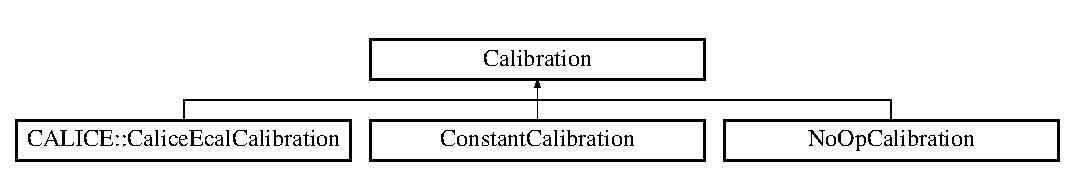
\includegraphics[height=1.93437cm]{classCalibration}
\end{center}
\end{figure}
\subsection*{Public Member Functions}
\begin{DoxyCompactItemize}
\item 
virtual Float\_\-t {\bf getCalibratedValue} (UInt\_\-t module\_\-id, UInt\_\-t module\_\-type, UInt\_\-t cell\_\-index, Float\_\-t adc\_\-value) const =0
\begin{DoxyCompactList}\small\item\em Determine from a pedestal subtracted ADC value a calibrated value. \item\end{DoxyCompactList}\item 
virtual Bool\_\-t {\bf isValid} (UInt\_\-t module\_\-id, UInt\_\-t module\_\-type, UInt\_\-t cell\_\-index) const 
\begin{DoxyCompactList}\small\item\em Return true if a the calibration constants for the given cell are in the allowed range. \item\end{DoxyCompactList}\item 
virtual Bool\_\-t {\bf checkForCalibrationConstantsOfModule} (UInt\_\-t module\_\-id, UInt\_\-t module\_\-type, UInt\_\-t n\_\-cells) const =0
\begin{DoxyCompactList}\small\item\em Verify that calibration constants exist for a certain module. \item\end{DoxyCompactList}\item 
virtual Int\_\-t {\bf getMiniumADCForMipThreshold} (Float\_\-t mip\_\-energy\_\-fraction) const =0
\begin{DoxyCompactList}\small\item\em Get the minimum adc value mips will have for the given energy fraction on all pads. \item\end{DoxyCompactList}\end{DoxyCompactItemize}


\subsection{Detailed Description}
Abstract interface of a calibration object. The calibration object returns for a value measured with a certain cell a calibrated value. 

Definition at line 9 of file Calibration.hh.

\subsection{Member Function Documentation}
\index{Calibration@{Calibration}!checkForCalibrationConstantsOfModule@{checkForCalibrationConstantsOfModule}}
\index{checkForCalibrationConstantsOfModule@{checkForCalibrationConstantsOfModule}!Calibration@{Calibration}}
\subsubsection[{checkForCalibrationConstantsOfModule}]{\setlength{\rightskip}{0pt plus 5cm}virtual Bool\_\-t Calibration::checkForCalibrationConstantsOfModule (UInt\_\-t {\em module\_\-id}, \/  UInt\_\-t {\em module\_\-type}, \/  UInt\_\-t {\em n\_\-cells}) const\hspace{0.3cm}{\ttfamily  [pure virtual]}}\label{classCalibration_a04c8f21c6e77cd3c91c858ca2c9373c4}


Verify that calibration constants exist for a certain module. 
\begin{DoxyParams}{Parameters}
\item[{\em module\_\-id}]id Or serial number of a module which uniquely identifies a detector module of a certain type. \item[{\em module\_\-type}]the type of the detector module \item[{\em n\_\-cells}]the number of cells on this module. Return true if calibration constants exist for the given module and the number of cells matches the number of calibration constants. \end{DoxyParams}


Implemented in {\bf ConstantCalibration} \doxyref{}{p.}{classConstantCalibration_aec30f5342ec651fa61708d2675e14d05}, and {\bf NoOpCalibration} \doxyref{}{p.}{classNoOpCalibration_acdb31ec76cef7720c0cda5fb15ffa2fb}.

Referenced by CALICE::SimpleHitSearch::buildCellParameters().\index{Calibration@{Calibration}!getCalibratedValue@{getCalibratedValue}}
\index{getCalibratedValue@{getCalibratedValue}!Calibration@{Calibration}}
\subsubsection[{getCalibratedValue}]{\setlength{\rightskip}{0pt plus 5cm}virtual Float\_\-t Calibration::getCalibratedValue (UInt\_\-t {\em module\_\-id}, \/  UInt\_\-t {\em module\_\-type}, \/  UInt\_\-t {\em cell\_\-index}, \/  Float\_\-t {\em adc\_\-value}) const\hspace{0.3cm}{\ttfamily  [pure virtual]}}\label{classCalibration_aca88d93a445ba3021c05dd61b293568c}


Determine from a pedestal subtracted ADC value a calibrated value. 
\begin{DoxyParams}{Parameters}
\item[{\em module\_\-id}]id Or serial number of a module which uniquely identifies a detector module of a certain type. \item[{\em module\_\-type}]the type of the detector module \item[{\em cell\_\-index}]the cell\_\-index in read order: first the ADC values of the first sample from all chips, then the next sample ... \item[{\em adc\_\-value}]the ADC value which should be calibrated. \end{DoxyParams}
\begin{DoxyReturn}{Returns}
the calibrated value. 
\end{DoxyReturn}


Implemented in {\bf ConstantCalibration} \doxyref{}{p.}{classConstantCalibration_a347808435c2c9e499af4c9a83d1c6915}, and {\bf NoOpCalibration} \doxyref{}{p.}{classNoOpCalibration_a8dd43819c4e5bb09e097f4db360a57fe}.

Referenced by CALICE::CalibrateAndApplyThreshold::processEvent().\index{Calibration@{Calibration}!getMiniumADCForMipThreshold@{getMiniumADCForMipThreshold}}
\index{getMiniumADCForMipThreshold@{getMiniumADCForMipThreshold}!Calibration@{Calibration}}
\subsubsection[{getMiniumADCForMipThreshold}]{\setlength{\rightskip}{0pt plus 5cm}virtual Int\_\-t Calibration::getMiniumADCForMipThreshold (Float\_\-t {\em mip\_\-energy\_\-fraction}) const\hspace{0.3cm}{\ttfamily  [pure virtual]}}\label{classCalibration_a4e45f1eca0d4fdf19ad76b8f581aee12}


Get the minimum adc value mips will have for the given energy fraction on all pads. 
\begin{DoxyParams}{Parameters}
\item[{\em mip\_\-energy\_\-fraction}]the energy in mips \end{DoxyParams}
\begin{DoxyReturn}{Returns}
minimum adc value which is below the given energy on all pads. This method can be used to get the lowest adc value a mip of the given energy fraction will have on all pads. This value is useful to select candidates before actually performing th calibration. This function is intended to be called at the beginning of each event. 
\end{DoxyReturn}


Implemented in {\bf ConstantCalibration} \doxyref{}{p.}{classConstantCalibration_ada035fed7a513d3da391bdea2c1d23f7}, and {\bf NoOpCalibration} \doxyref{}{p.}{classNoOpCalibration_a8b478c6680b5980c2b87cedc8a589989}.

Referenced by CALICE::CalibrateAndApplyThreshold::processEvent(), CALICE::SimpleHitSearch::searchHits(), and CALICE::SimpleHitSearch::searchHitsAndAdjustPedestalsAndNoise().\index{Calibration@{Calibration}!isValid@{isValid}}
\index{isValid@{isValid}!Calibration@{Calibration}}
\subsubsection[{isValid}]{\setlength{\rightskip}{0pt plus 5cm}virtual Bool\_\-t Calibration::isValid (UInt\_\-t {\em module\_\-id}, \/  UInt\_\-t {\em module\_\-type}, \/  UInt\_\-t {\em cell\_\-index}) const\hspace{0.3cm}{\ttfamily  [inline, virtual]}}\label{classCalibration_a7d516d7b66b1f20640829d12adfd64d6}


Return true if a the calibration constants for the given cell are in the allowed range. 
\begin{DoxyParams}{Parameters}
\item[{\em module\_\-id}]id Or serial number of a module which uniquely identifies a detector module of a certain type. \item[{\em module\_\-type}]the type of the detector module \item[{\em cell\_\-index}]the cell\_\-index in read order: first the ADC values of the first sample from all chips, then the next sample ... \end{DoxyParams}
\begin{DoxyReturn}{Returns}
true for cells with valid calibration constants, false for cells which should be declared dead.
\end{DoxyReturn}
This method is used to find, after module connection changes, cells which should be declared dead. 

Definition at line 31 of file Calibration.hh.

Referenced by CALICE::SimpleHitSearch::buildCellParameters(), CALICE::CalibrateAndApplyThreshold::processRunHeader(), CALICE::SimpleHitSearch::resetForInitialPedestalNoiseCalculation(), and CALICE::SimpleHitSearch::resetForPedestalNoiseReCalculation().

The documentation for this class was generated from the following file:\begin{DoxyCompactItemize}
\item 
Calibration.hh\end{DoxyCompactItemize}

\section{CalibrationFactory Class Reference}
\label{classCalibrationFactory}\index{CalibrationFactory@{CalibrationFactory}}


Return a calibration object of the given name.  


{\ttfamily \#include $<$CalibrationFactory.hh$>$}\subsection*{Public Member Functions}
\begin{DoxyCompactItemize}
\item 
void {\bf registerCalibrationKit} (const std::string \&kit\_\-name, {\bf CalibrationKit} $\ast$a\_\-kit)\label{classCalibrationFactory_ae3f5c6f7204526d98c753dac871e8217}

\begin{DoxyCompactList}\small\item\em Register a \doxyref{Calibration}{p.}{classCalibration} object kit. \item\end{DoxyCompactList}\item 
{\bf Calibration} $\ast$ {\bf createCalibrationObject} (const std::string \&name, const std::string \&module\_\-type\_\-col\_\-name, const std::string \&module\_\-calibration\_\-col\_\-name)  throw (std::runtime\_\-error)\label{classCalibrationFactory_a8f74cdd3b9dffc44752f211743f6a74c}

\begin{DoxyCompactList}\small\item\em Get an object for the calibration. \item\end{DoxyCompactList}\item 
void {\bf listKits} ()
\begin{DoxyCompactList}\small\item\em Show all registered kits. \item\end{DoxyCompactList}\end{DoxyCompactItemize}
\subsection*{Static Public Member Functions}
\begin{DoxyCompactItemize}
\item 
static {\bf CalibrationFactory} $\ast$ {\bf getInstance} ()\label{classCalibrationFactory_a5efb95a0d951b8da5a8bdb5832a9831d}

\begin{DoxyCompactList}\small\item\em Get the global instance of the \doxyref{Calibration}{p.}{classCalibration} Object Factory. \item\end{DoxyCompactList}\end{DoxyCompactItemize}
\subsection*{Private Attributes}
\begin{DoxyCompactItemize}
\item 
std::map$<$ std::string, {\bf CalibrationKit} $\ast$ $>$ {\bf \_\-kits}
\begin{DoxyCompactList}\small\item\em List of registered \doxyref{Calibration}{p.}{classCalibration} kits. \item\end{DoxyCompactList}\end{DoxyCompactItemize}
\subsection*{Static Private Attributes}
\begin{DoxyCompactItemize}
\item 
static {\bf CalibrationFactory} $\ast$ {\bf \_\-\_\-instance} = 0
\begin{DoxyCompactList}\small\item\em Pointer to the global \doxyref{CalibrationFactory}{p.}{classCalibrationFactory} instance. \item\end{DoxyCompactList}\end{DoxyCompactItemize}


\subsection{Detailed Description}
Return a calibration object of the given name. \doxyref{Calibration}{p.}{classCalibration} kits are registered with a certain name. This name which is for example specified by a Marlin parameter can than be used to create the actual calibration object. 

Definition at line 16 of file CalibrationFactory.hh.

\subsection{Member Function Documentation}
\index{CalibrationFactory@{CalibrationFactory}!listKits@{listKits}}
\index{listKits@{listKits}!CalibrationFactory@{CalibrationFactory}}
\subsubsection[{listKits}]{\setlength{\rightskip}{0pt plus 5cm}void CalibrationFactory::listKits ()}\label{classCalibrationFactory_a8ec8e4dacbc4b38c7fd760b7b00857d3}


Show all registered kits. For debugging. 

Definition at line 6 of file CalibrationFactory.cc.

References \_\-kits.

Referenced by CALICE::SimpleHitSearch::init(), and CALICE::CalibrateAndApplyThreshold::init().

\subsection{Field Documentation}
\index{CalibrationFactory@{CalibrationFactory}!\_\-\_\-instance@{\_\-\_\-instance}}
\index{\_\-\_\-instance@{\_\-\_\-instance}!CalibrationFactory@{CalibrationFactory}}
\subsubsection[{\_\-\_\-instance}]{\setlength{\rightskip}{0pt plus 5cm}{\bf CalibrationFactory} $\ast$ {\bf CalibrationFactory::\_\-\_\-instance} = 0\hspace{0.3cm}{\ttfamily  [static, private]}}\label{classCalibrationFactory_a19b2dfab32cd94981a00a8f39e9b028b}


Pointer to the global \doxyref{CalibrationFactory}{p.}{classCalibrationFactory} instance. 

Definition at line 64 of file CalibrationFactory.hh.

Referenced by getInstance().\index{CalibrationFactory@{CalibrationFactory}!\_\-kits@{\_\-kits}}
\index{\_\-kits@{\_\-kits}!CalibrationFactory@{CalibrationFactory}}
\subsubsection[{\_\-kits}]{\setlength{\rightskip}{0pt plus 5cm}std::map$<$std::string, {\bf CalibrationKit} $\ast$$>$ {\bf CalibrationFactory::\_\-kits}\hspace{0.3cm}{\ttfamily  [private]}}\label{classCalibrationFactory_a2ff2373b183b599ef137ee6f19e1fa6e}


List of registered \doxyref{Calibration}{p.}{classCalibration} kits. 

Definition at line 63 of file CalibrationFactory.hh.

Referenced by createCalibrationObject(), listKits(), and registerCalibrationKit().

The documentation for this class was generated from the following files:\begin{DoxyCompactItemize}
\item 
CalibrationFactory.hh\item 
CalibrationFactory.cc\end{DoxyCompactItemize}

\section{CalibrationKit Class Reference}
\label{classCalibrationKit}\index{CalibrationKit@{CalibrationKit}}


Abstract interface of a calibration kit which can create calibration objects.  


{\ttfamily \#include $<$CalibrationKit.hh$>$}Inheritance diagram for CalibrationKit::\begin{figure}[H]
\begin{center}
\leavevmode
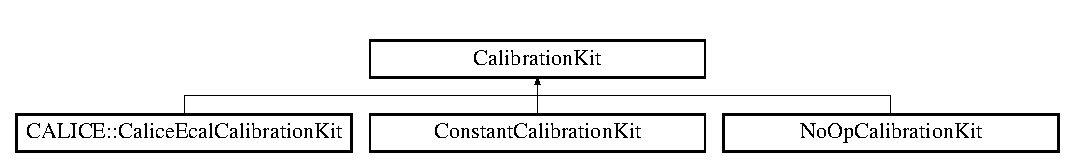
\includegraphics[height=1.80354cm]{classCalibrationKit}
\end{center}
\end{figure}
\subsection*{Public Member Functions}
\begin{DoxyCompactItemize}
\item 
virtual {\bf Calibration} $\ast$ {\bf create} (const std::string \&module\_\-type\_\-col\_\-name, const std::string \&module\_\-calibration\_\-col\_\-name) const =0
\begin{DoxyCompactList}\small\item\em create calibration object. \item\end{DoxyCompactList}\end{DoxyCompactItemize}


\subsection{Detailed Description}
Abstract interface of a calibration kit which can create calibration objects. 

Definition at line 11 of file CalibrationKit.hh.

\subsection{Member Function Documentation}
\index{CalibrationKit@{CalibrationKit}!create@{create}}
\index{create@{create}!CalibrationKit@{CalibrationKit}}
\subsubsection[{create}]{\setlength{\rightskip}{0pt plus 5cm}virtual {\bf Calibration}$\ast$ CalibrationKit::create (const std::string \& {\em module\_\-type\_\-col\_\-name}, \/  const std::string \& {\em module\_\-calibration\_\-col\_\-name}) const\hspace{0.3cm}{\ttfamily  [pure virtual]}}\label{classCalibrationKit_ab3aea5671d91a7b6f5e839324cf45a70}


create calibration object. 
\begin{DoxyParams}{Parameters}
\item[{\em module\_\-type\_\-col\_\-name}]the name of the conditions data collection with the module types. \item[{\em module\_\-calibration\_\-col\_\-name}]the name of the conditions data collection which contains the calibration constants. FIXME: There should be a better method to hand parameters to \doxyref{Calibration}{p.}{classCalibration} objects. \end{DoxyParams}


Implemented in {\bf CALICE::CaliceEcalCalibrationKit} \doxyref{}{p.}{classCALICE_1_1CaliceEcalCalibrationKit_aa8754032807fe2e3d7d8dc4225464829}, {\bf ConstantCalibrationKit} \doxyref{}{p.}{classConstantCalibrationKit_a3b84989011be10b816104fdc58963882}, and {\bf NoOpCalibrationKit} \doxyref{}{p.}{classNoOpCalibrationKit_ac197f7bf5528b484d5b70e664655474b}.

The documentation for this class was generated from the following file:\begin{DoxyCompactItemize}
\item 
CalibrationKit.hh\end{DoxyCompactItemize}

\section{CALICE::CalibrationSet$<$ T $>$ Class Template Reference}
\label{classCALICE_1_1CalibrationSet}\index{CALICE::CalibrationSet@{CALICE::CalibrationSet}}


Class which handles the storage of a set of LCHcalCalibrationObject.  


{\ttfamily \#include $<$CalibrationSet.hh$>$}\subsection*{Public Types}
\begin{DoxyCompactItemize}
\item 
typedef std::map$<$ unsigned, T $\ast$ $>$ {\bfseries CalibModuleMap}\label{classCALICE_1_1CalibrationSet_ae0ef8d231d149d1e61a4000952d58d67}

\item 
typedef std::pair$<$ lcio::LCCollection $\ast$, CalibModuleMap $\ast$ $>$ {\bfseries CalibModuleData}\label{classCALICE_1_1CalibrationSet_a894d8c42a35b66022bb221db4585f5f5}

\item 
typedef std::map$<$ unsigned, CalibModuleData $>$ {\bfseries CalibReadMap}\label{classCALICE_1_1CalibrationSet_a6f4a5967aa3a3ad50d763a92809fcf60}

\end{DoxyCompactItemize}
\subsection*{Public Member Functions}
\begin{DoxyCompactItemize}
\item 
{\bfseries CalibrationSet} ({\bf TempModel} $\ast$tempModel)\label{classCALICE_1_1CalibrationSet_a5b3dc2a9fee4bb05ead1f6aecb63e508}

\item 
bool {\bfseries empty} ()\label{classCALICE_1_1CalibrationSet_acf72ce0c2908ad7c57c1a4fed2e0ae69}

\item 
void {\bfseries fill} (lcio::LCCollection $\ast$calCol)\label{classCALICE_1_1CalibrationSet_af6eada4b282e59cd26830121ffe431ad}

\item 
void {\bfseries fill} (lcio::LCCollection $\ast$calCol, lcio::LCCollection $\ast$sroCol)\label{classCALICE_1_1CalibrationSet_a5064acda09ac4e6f60dfd8c95575bb77}

\item 
T $\ast$ {\bfseries getCalib} (unsigned moduleID, unsigned cellKey)\label{classCALICE_1_1CalibrationSet_ab7ccb1fe35ac7634ea52412ae96da4e5}

\item 
T $\ast$ {\bfseries getCalib} (unsigned module, unsigned chip, unsigned channel)\label{classCALICE_1_1CalibrationSet_a0e439372aeaa7d78b6fbcf0886022f1e}

\item 
void {\bfseries setTemp} (lcio::LCCollection $\ast$sroCol)\label{classCALICE_1_1CalibrationSet_a5dcbfc885e768814df5ffb3309173322}

\item 
void {\bfseries applyScalingFactor} (float f)\label{classCALICE_1_1CalibrationSet_aba2e28745da6330c981810dd5e21f0ae}

\item 
void {\bfseries setScalingFactor} (float f)\label{classCALICE_1_1CalibrationSet_aefc2753764d779cd34362c8a5f8b6943}

\end{DoxyCompactItemize}
\subsection*{Data Fields}
\begin{DoxyCompactItemize}
\item 
CalibReadMap {\bfseries \_\-readMap}\label{classCALICE_1_1CalibrationSet_a57c533ff2868f73cf2029d32568b3e20}

\item 
{\bf TempModel} $\ast$ {\bfseries \_\-tempModel}\label{classCALICE_1_1CalibrationSet_a1076b184fc1d2ae4bb05f204fbe07f34}

\end{DoxyCompactItemize}
\subsection*{Private Attributes}
\begin{DoxyCompactItemize}
\item 
float {\bfseries \_\-scalingFactor}\label{classCALICE_1_1CalibrationSet_a6e4301d0f06d4afd7747c55cc1d72755}

\end{DoxyCompactItemize}


\subsection{Detailed Description}
\subsubsection*{template$<$class T$>$ class CALICE::CalibrationSet$<$ T $>$}

Class which handles the storage of a set of LCHcalCalibrationObject. \begin{DoxyAuthor}{Author}
S.Schmidt, DESY 
\end{DoxyAuthor}
\begin{DoxyDate}{Date}
Jun 15 2007 
\end{DoxyDate}


Definition at line 28 of file CalibrationSet.hh.

The documentation for this class was generated from the following file:\begin{DoxyCompactItemize}
\item 
CalibrationSet.hh\end{DoxyCompactItemize}

\section{marlin::CaliceConditionsDataCreator Class Reference}
\label{classmarlin_1_1CaliceConditionsDataCreator}\index{marlin::CaliceConditionsDataCreator@{marlin::CaliceConditionsDataCreator}}


Marlin processr which creates calice conditions data and makes them via a simplefile handler available.  


{\ttfamily \#include $<$CaliceConditionsDataCreator.hh$>$}\subsection*{Public Member Functions}
\begin{DoxyCompactItemize}
\item 
Processor $\ast$ {\bfseries newProcessor} ()\label{classmarlin_1_1CaliceConditionsDataCreator_a602c419bdb5c11770dd620711941f175}

\item 
void {\bf init} ()
\begin{DoxyCompactList}\small\item\em Install conditions change listener. \item\end{DoxyCompactList}\item 
void {\bfseries processRunHeader} (LCRunHeader $\ast$run)\label{classmarlin_1_1CaliceConditionsDataCreator_add37acebb16fb3faa09f17afa353ad6a}

\item 
void {\bf processEvent} (LCEvent $\ast$evtP)\label{classmarlin_1_1CaliceConditionsDataCreator_a1a7b0067f58a6376ab5e9ba73d389280}

\begin{DoxyCompactList}\small\item\em Update conditions data (not yet). \item\end{DoxyCompactList}\item 
void {\bfseries end} ()\label{classmarlin_1_1CaliceConditionsDataCreator_a7903f04212f4cbb7f95fecd657c289f0}

\end{DoxyCompactItemize}
\subsection*{Protected Types}
\begin{DoxyCompactItemize}
\item 
enum \{ \par
{\bfseries kAhcModuleLocation}, 
{\bfseries kAhcModuleConnection}, 
{\bfseries kAhcModuleDescription}, 
{\bfseries kEmcModuleLocation}, 
\par
{\bfseries kEmcModuleConnection}, 
{\bfseries kEmcModuleDescription}, 
{\bfseries kDriftChamberParameter}, 
{\bfseries kTriggerAssignment}, 
\par
{\bfseries kTriggerCheck}, 
{\bfseries kExperimentalSetup}, 
{\bfseries kNCollections}
 \}
\end{DoxyCompactItemize}
\subsection*{Protected Attributes}
\begin{DoxyCompactItemize}
\item 
std::string {\bfseries \_\-colName} [kNCollections]\label{classmarlin_1_1CaliceConditionsDataCreator_a1c7c2ec9238554a06a8850b0679b66f9}

\item 
std::vector$<$ std::string $>$ {\bfseries \_\-inputFileName} [kNCollections]\label{classmarlin_1_1CaliceConditionsDataCreator_a91361a635c7673038c4482ad8209f639}

\item 
std::vector$<$ std::string $>$ {\bfseries \_\-sinceTillTime} [kNCollections]\label{classmarlin_1_1CaliceConditionsDataCreator_a5dd2783bec7e29c83911b2c62a5733ea}

\item 
std::vector$<$ UTIL::LCTime $>$ {\bfseries \_\-since} [kNCollections]\label{classmarlin_1_1CaliceConditionsDataCreator_afb8943272775c52775822d64f0445505}

\item 
std::vector$<$ UTIL::LCTime $>$ {\bfseries \_\-till} [kNCollections]\label{classmarlin_1_1CaliceConditionsDataCreator_a6c8842188702a4d711ece614f93c0d88}

\item 
std::vector$<$ std::string $>$ {\bf \_\-beamType}
\begin{DoxyCompactList}\small\item\em the nominal beam type. \item\end{DoxyCompactList}\item 
std::vector$<$ float $>$ {\bf \_\-beamEnergy}
\begin{DoxyCompactList}\small\item\em nominal beam energy. \item\end{DoxyCompactList}\item 
std::vector$<$ float $>$ {\bf \_\-configurationAngle}
\begin{DoxyCompactList}\small\item\em angle between the detector normal and the beam axis. \item\end{DoxyCompactList}\item 
std::vector$<$ int $>$ {\bf \_\-triggerMainWord}
\begin{DoxyCompactList}\small\item\em position of the trigger main word in th fifo. \item\end{DoxyCompactList}\item 
std::vector$<$ int $>$ {\bf \_\-triggerMainWordTolerance}\label{classmarlin_1_1CaliceConditionsDataCreator_ae121828e72a6e69229ea1102e3cacc4c}

\begin{DoxyCompactList}\small\item\em the tolerance on the trigger main word position \item\end{DoxyCompactList}\item 
std::vector$<$ int $>$ {\bf \_\-triggerSearchRange}
\begin{DoxyCompactList}\small\item\em search range around the trigger main word which is search for overlapping triggers. \item\end{DoxyCompactList}\item 
lccd::IConditionsHandler $\ast$ {\bfseries \_\-conddbHandler} [kNCollections]\label{classmarlin_1_1CaliceConditionsDataCreator_ac99c9b4383bf7e786b763f5789147b1c}

\item 
std::vector$<$ EVENT::LCCollection $\ast$ $>$ {\bfseries \_\-conddbCol} [kNCollections]\label{classmarlin_1_1CaliceConditionsDataCreator_a115c3f1d7deec6ab19666acff4be962e}

\item 
UTIL::LCTime {\bfseries \_\-validSince}\label{classmarlin_1_1CaliceConditionsDataCreator_aa0271519445413603682631355db7a63}

\item 
UTIL::LCTime {\bfseries \_\-validTill}\label{classmarlin_1_1CaliceConditionsDataCreator_a39ed98e58fe973f45aedbbf64a3aef2e}

\end{DoxyCompactItemize}
\subsection*{Static Protected Attributes}
\begin{DoxyCompactItemize}
\item 
static const char $\ast$ {\bfseries \_\-\_\-beamTypeNames} [11]\label{classmarlin_1_1CaliceConditionsDataCreator_a86e1060f18685fd8e77e84a396b9004f}

\item 
static const char $\ast$ {\bfseries \_\-\_\-collectionNames} [kNCollections]\label{classmarlin_1_1CaliceConditionsDataCreator_a828d149c7eaaa7c07aa28ccd2bcffd69}

\item 
static CreateCollFunc\_\-t {\bfseries \_\-\_\-createFunc} [kNCollections]\label{classmarlin_1_1CaliceConditionsDataCreator_a50bb1fc9365a24fde378c286a30cd47b}

\end{DoxyCompactItemize}
\subsection*{Friends}
\begin{DoxyCompactItemize}
\item 
class {\bfseries CALICE::ConditionsDataWriteHandler}\label{classmarlin_1_1CaliceConditionsDataCreator_a0e401bb1bfedeba5808934499877adf4}

\end{DoxyCompactItemize}


\subsection{Detailed Description}
Marlin processr which creates calice conditions data and makes them via a simplefile handler available. The processor creates: 
\begin{DoxyEnumerate}
\item ModuleConnection 
\item ModuleLocation 
\item ModuleDescription 
\item DriftChamberParameter 
\item ExperimentalSetup 
\item TriggerAssignament 
\end{DoxyEnumerate}collections. The creation of each collection can be individually steered. 

Definition at line 39 of file CaliceConditionsDataCreator.hh.

\subsection{Member Function Documentation}
\index{marlin::CaliceConditionsDataCreator@{marlin::CaliceConditionsDataCreator}!init@{init}}
\index{init@{init}!marlin::CaliceConditionsDataCreator@{marlin::CaliceConditionsDataCreator}}
\subsubsection[{init}]{\setlength{\rightskip}{0pt plus 5cm}void marlin::CaliceConditionsDataCreator::init ()}\label{classmarlin_1_1CaliceConditionsDataCreator_a53e34b9c420e45dda6bbab5f9f4400cc}


Install conditions change listener. The listeners are installed for the conditions data specified by the processor parameters. 

\subsection{Field Documentation}
\index{marlin::CaliceConditionsDataCreator@{marlin::CaliceConditionsDataCreator}!\_\-beamEnergy@{\_\-beamEnergy}}
\index{\_\-beamEnergy@{\_\-beamEnergy}!marlin::CaliceConditionsDataCreator@{marlin::CaliceConditionsDataCreator}}
\subsubsection[{\_\-beamEnergy}]{\setlength{\rightskip}{0pt plus 5cm}std::vector$<$float$>$ {\bf marlin::CaliceConditionsDataCreator::\_\-beamEnergy}\hspace{0.3cm}{\ttfamily  [protected]}}\label{classmarlin_1_1CaliceConditionsDataCreator_af8aa319f5771ba7bfcf4c3be1c36cf4f}


nominal beam energy. 

Definition at line 75 of file CaliceConditionsDataCreator.hh.\index{marlin::CaliceConditionsDataCreator@{marlin::CaliceConditionsDataCreator}!\_\-beamType@{\_\-beamType}}
\index{\_\-beamType@{\_\-beamType}!marlin::CaliceConditionsDataCreator@{marlin::CaliceConditionsDataCreator}}
\subsubsection[{\_\-beamType}]{\setlength{\rightskip}{0pt plus 5cm}std::vector$<$std::string$>$ {\bf marlin::CaliceConditionsDataCreator::\_\-beamType}\hspace{0.3cm}{\ttfamily  [protected]}}\label{classmarlin_1_1CaliceConditionsDataCreator_a0c0658ad562522454b5c278757e02118}


the nominal beam type. 

Definition at line 74 of file CaliceConditionsDataCreator.hh.\index{marlin::CaliceConditionsDataCreator@{marlin::CaliceConditionsDataCreator}!\_\-configurationAngle@{\_\-configurationAngle}}
\index{\_\-configurationAngle@{\_\-configurationAngle}!marlin::CaliceConditionsDataCreator@{marlin::CaliceConditionsDataCreator}}
\subsubsection[{\_\-configurationAngle}]{\setlength{\rightskip}{0pt plus 5cm}std::vector$<$float$>$ {\bf marlin::CaliceConditionsDataCreator::\_\-configurationAngle}\hspace{0.3cm}{\ttfamily  [protected]}}\label{classmarlin_1_1CaliceConditionsDataCreator_ae54f3d9bb7f189e2b888c1f3a5aac59c}


angle between the detector normal and the beam axis. 

Definition at line 76 of file CaliceConditionsDataCreator.hh.\index{marlin::CaliceConditionsDataCreator@{marlin::CaliceConditionsDataCreator}!\_\-triggerMainWord@{\_\-triggerMainWord}}
\index{\_\-triggerMainWord@{\_\-triggerMainWord}!marlin::CaliceConditionsDataCreator@{marlin::CaliceConditionsDataCreator}}
\subsubsection[{\_\-triggerMainWord}]{\setlength{\rightskip}{0pt plus 5cm}std::vector$<$int$>$ {\bf marlin::CaliceConditionsDataCreator::\_\-triggerMainWord}\hspace{0.3cm}{\ttfamily  [protected]}}\label{classmarlin_1_1CaliceConditionsDataCreator_a0459f44af2be6a6c11e129ec7a0f053c}


position of the trigger main word in th fifo. 

Definition at line 78 of file CaliceConditionsDataCreator.hh.\index{marlin::CaliceConditionsDataCreator@{marlin::CaliceConditionsDataCreator}!\_\-triggerSearchRange@{\_\-triggerSearchRange}}
\index{\_\-triggerSearchRange@{\_\-triggerSearchRange}!marlin::CaliceConditionsDataCreator@{marlin::CaliceConditionsDataCreator}}
\subsubsection[{\_\-triggerSearchRange}]{\setlength{\rightskip}{0pt plus 5cm}std::vector$<$int$>$ {\bf marlin::CaliceConditionsDataCreator::\_\-triggerSearchRange}\hspace{0.3cm}{\ttfamily  [protected]}}\label{classmarlin_1_1CaliceConditionsDataCreator_a0e3e6e12b1a9177d4c233719db4978ca}


search range around the trigger main word which is search for overlapping triggers. 

Definition at line 80 of file CaliceConditionsDataCreator.hh.

The documentation for this class was generated from the following file:\begin{DoxyCompactItemize}
\item 
CaliceConditionsDataCreator.hh\end{DoxyCompactItemize}

\section{CALICE::CaliceEcalCalibration Class Reference}
\label{classCALICE_1_1CaliceEcalCalibration}\index{CALICE::CaliceEcalCalibration@{CALICE::CaliceEcalCalibration}}


\doxyref{Calibration}{p.}{classCalibration} of the Calice ECAL modules.  


{\ttfamily \#include $<$CaliceEcalCalibration.hh$>$}Inheritance diagram for CALICE::CaliceEcalCalibration::\begin{figure}[H]
\begin{center}
\leavevmode
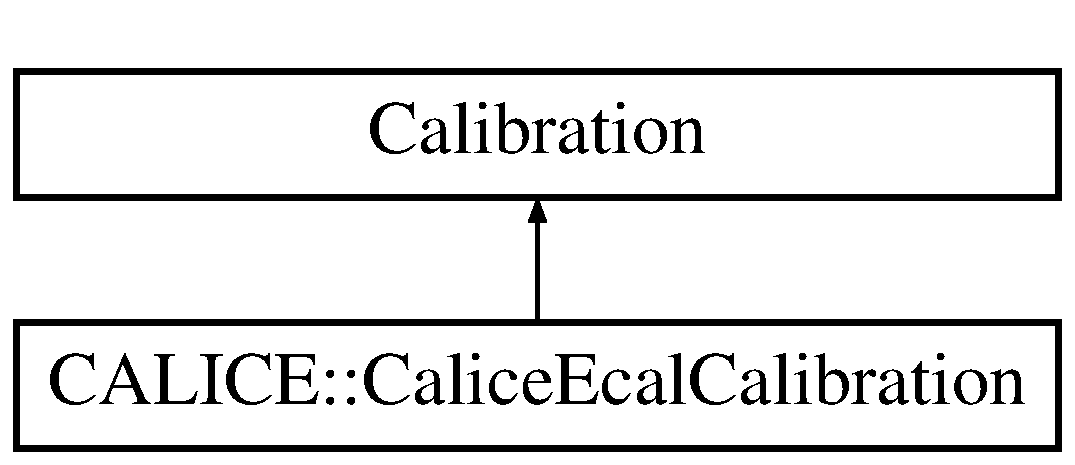
\includegraphics[height=2cm]{classCALICE_1_1CaliceEcalCalibration}
\end{center}
\end{figure}
\subsection*{Public Member Functions}
\begin{DoxyCompactItemize}
\item 
{\bf CaliceEcalCalibration} (const std::string \&module\_\-type\_\-col\_\-name, const std::string \&calibration\_\-constants\_\-col\_\-name)  throw (std::runtime\_\-error)
\begin{DoxyCompactList}\small\item\em Create the calibration object for the Calice Ecal. \item\end{DoxyCompactList}\item 
{\bf $\sim$CaliceEcalCalibration} ()
\begin{DoxyCompactList}\small\item\em Destructor. \item\end{DoxyCompactList}\item 
Float\_\-t {\bf getCalibratedValue} (UInt\_\-t module\_\-id, UInt\_\-t module\_\-type, UInt\_\-t cell\_\-index, Float\_\-t adc\_\-value) const 
\begin{DoxyCompactList}\small\item\em Determine from a pedestal subtracted ADC value a calibrated value. \item\end{DoxyCompactList}\item 
Bool\_\-t {\bf isValid} (UInt\_\-t module\_\-id, UInt\_\-t module\_\-type, UInt\_\-t cell\_\-index) const 
\begin{DoxyCompactList}\small\item\em Return true if a the calibration constants for the given cell are in the allowed range. \item\end{DoxyCompactList}\item 
Bool\_\-t {\bf checkForCalibrationConstantsOfModule} (UInt\_\-t module\_\-id, UInt\_\-t module\_\-type, UInt\_\-t n\_\-cells) const 
\begin{DoxyCompactList}\small\item\em Verify that calibration constants exist for a certain module. \item\end{DoxyCompactList}\item 
Int\_\-t {\bf getMiniumADCForMipThreshold} (Float\_\-t mip\_\-energy\_\-fraction) const 
\begin{DoxyCompactList}\small\item\em Get the minimum adc value mips will have for the given energy fraction on all pads. \item\end{DoxyCompactList}\item 
void {\bf moduleTypeChanged} (lcio::LCCollection $\ast$col)
\begin{DoxyCompactList}\small\item\em Notify the calibration object in case the definition of the module types has changed. \item\end{DoxyCompactList}\item 
void {\bf calibrationConstantChanged} (lcio::LCCollection $\ast$col)
\begin{DoxyCompactList}\small\item\em Notify the calibration object when ever the calibration constants change. \item\end{DoxyCompactList}\end{DoxyCompactItemize}
\subsection*{Private Types}
\begin{DoxyCompactItemize}
\item 
typedef std::vector$<$ EcalModuleCalibration $>$ {\bfseries ModuleTypeCalibrationConstantList\_\-t}\label{classCALICE_1_1CaliceEcalCalibration_a7c5d9af5b11b804071982e5292422646}

\item 
typedef std::vector$<$ std::pair$<$ const ModuleTypeCalibrationConstantList\_\-t $\ast$, std::string $>$ $>$ {\bfseries CalibrationConstantPerTypeList\_\-t}\label{classCALICE_1_1CaliceEcalCalibration_aab75d417a8477f123384473c932b1d3e}

\end{DoxyCompactItemize}
\subsection*{Private Attributes}
\begin{DoxyCompactItemize}
\item 
std::map$<$ std::string, ModuleTypeCalibrationConstantList\_\-t $>$ {\bfseries \_\-calibrationConstants}\label{classCALICE_1_1CaliceEcalCalibration_a3a4ba7bfc9da0dcae8acc075f74eff24}

\item 
CalibrationConstantPerTypeList\_\-t {\bf \_\-calibrationConstantsPerType}
\begin{DoxyCompactList}\small\item\em \doxyref{Calibration}{p.}{classCalibration} constatns per Module. \item\end{DoxyCompactList}\item 
ConditionsChangeDelegator$<$ {\bf CaliceEcalCalibration} $>$ {\bfseries \_\-moduleTypeChange}\label{classCALICE_1_1CaliceEcalCalibration_a49a0c1cccc53314ec3e8e44a7186031d}

\item 
ConditionsChangeDelegator$<$ {\bf CaliceEcalCalibration} $>$ {\bfseries \_\-calibrationConstantChange}\label{classCALICE_1_1CaliceEcalCalibration_a3c8999e65ff7276c3acdeb7b19eeea0c}

\item 
Float\_\-t {\bfseries \_\-minInvCalibrationConstant}\label{classCALICE_1_1CaliceEcalCalibration_ac9690f336fa6c193427f12d4504ad6b4}

\end{DoxyCompactItemize}
\subsection*{Static Private Attributes}
\begin{DoxyCompactItemize}
\item 
static EcalModuleCalibration {\bf \_\-empty}
\begin{DoxyCompactList}\small\item\em Used to initialise the vector. \item\end{DoxyCompactList}\end{DoxyCompactItemize}


\subsection{Detailed Description}
\doxyref{Calibration}{p.}{classCalibration} of the Calice ECAL modules. 

Definition at line 18 of file CaliceEcalCalibration.hh.

\subsection{Constructor \& Destructor Documentation}
\index{CALICE::CaliceEcalCalibration@{CALICE::CaliceEcalCalibration}!CaliceEcalCalibration@{CaliceEcalCalibration}}
\index{CaliceEcalCalibration@{CaliceEcalCalibration}!CALICE::CaliceEcalCalibration@{CALICE::CaliceEcalCalibration}}
\subsubsection[{CaliceEcalCalibration}]{\setlength{\rightskip}{0pt plus 5cm}CALICE::CaliceEcalCalibration::CaliceEcalCalibration (const std::string \& {\em module\_\-type\_\-col\_\-name}, \/  const std::string \& {\em calibration\_\-constants\_\-col\_\-name})  throw (std::runtime\_\-error)}\label{classCALICE_1_1CaliceEcalCalibration_ae18842d582f1c8acac63137903aa0bf7}


Create the calibration object for the Calice Ecal. The constructor will register handlers for conditions data changes: changes of the module types and the calibration constants. 

Definition at line 54 of file CaliceEcalCalibration.cc.\index{CALICE::CaliceEcalCalibration@{CALICE::CaliceEcalCalibration}!$\sim$CaliceEcalCalibration@{$\sim$CaliceEcalCalibration}}
\index{$\sim$CaliceEcalCalibration@{$\sim$CaliceEcalCalibration}!CALICE::CaliceEcalCalibration@{CALICE::CaliceEcalCalibration}}
\subsubsection[{$\sim$CaliceEcalCalibration}]{\setlength{\rightskip}{0pt plus 5cm}CALICE::CaliceEcalCalibration::$\sim$CaliceEcalCalibration ()\hspace{0.3cm}{\ttfamily  [inline]}}\label{classCALICE_1_1CaliceEcalCalibration_a90c221567561015797ff5c1b035dda71}


Destructor. FIXME: The destructor should deregister the conditions change handler. Unfortuneatly, this is not forseen in the Conditions Processor. 

Definition at line 32 of file CaliceEcalCalibration.hh.

\subsection{Member Function Documentation}
\index{CALICE::CaliceEcalCalibration@{CALICE::CaliceEcalCalibration}!calibrationConstantChanged@{calibrationConstantChanged}}
\index{calibrationConstantChanged@{calibrationConstantChanged}!CALICE::CaliceEcalCalibration@{CALICE::CaliceEcalCalibration}}
\subsubsection[{calibrationConstantChanged}]{\setlength{\rightskip}{0pt plus 5cm}void CALICE::CaliceEcalCalibration::calibrationConstantChanged (lcio::LCCollection $\ast$ {\em col})}\label{classCALICE_1_1CaliceEcalCalibration_a0a82a3215a4e35f444904cb80cea3f46}


Notify the calibration object when ever the calibration constants change. This function must be called at least once before \doxyref{getCalibratedValue()}{p.}{classCALICE_1_1CaliceEcalCalibration_a4ffba5606c463a2b7419e85bc9008853} is used. 

Definition at line 121 of file CaliceEcalCalibration.cc.

References \_\-calibrationConstantsPerType, and \_\-empty.\index{CALICE::CaliceEcalCalibration@{CALICE::CaliceEcalCalibration}!checkForCalibrationConstantsOfModule@{checkForCalibrationConstantsOfModule}}
\index{checkForCalibrationConstantsOfModule@{checkForCalibrationConstantsOfModule}!CALICE::CaliceEcalCalibration@{CALICE::CaliceEcalCalibration}}
\subsubsection[{checkForCalibrationConstantsOfModule}]{\setlength{\rightskip}{0pt plus 5cm}Bool\_\-t CALICE::CaliceEcalCalibration::checkForCalibrationConstantsOfModule (UInt\_\-t {\em module\_\-id}, \/  UInt\_\-t {\em module\_\-type}, \/  UInt\_\-t {\em n\_\-cells}) const\hspace{0.3cm}{\ttfamily  [inline]}}\label{classCALICE_1_1CaliceEcalCalibration_ae6cb1b990f7c4eb7dc274089df464772}


Verify that calibration constants exist for a certain module. 
\begin{DoxyParams}{Parameters}
\item[{\em module\_\-id}]id Or serial number of a module which uniquely identifies a detector module of a certain type. \item[{\em module\_\-type}]the type of the detector module \item[{\em n\_\-cells}]the number of cells on this module. Return true if calibration constants exist for the given module and the number of cells matches the number of calibration constants. \end{DoxyParams}


Definition at line 99 of file CaliceEcalCalibration.hh.

References \_\-calibrationConstantsPerType.\index{CALICE::CaliceEcalCalibration@{CALICE::CaliceEcalCalibration}!getCalibratedValue@{getCalibratedValue}}
\index{getCalibratedValue@{getCalibratedValue}!CALICE::CaliceEcalCalibration@{CALICE::CaliceEcalCalibration}}
\subsubsection[{getCalibratedValue}]{\setlength{\rightskip}{0pt plus 5cm}Float\_\-t CALICE::CaliceEcalCalibration::getCalibratedValue (UInt\_\-t {\em module\_\-id}, \/  UInt\_\-t {\em module\_\-type}, \/  UInt\_\-t {\em cell\_\-index}, \/  Float\_\-t {\em adc\_\-value}) const\hspace{0.3cm}{\ttfamily  [inline]}}\label{classCALICE_1_1CaliceEcalCalibration_a4ffba5606c463a2b7419e85bc9008853}


Determine from a pedestal subtracted ADC value a calibrated value. 
\begin{DoxyParams}{Parameters}
\item[{\em module\_\-id}]id Or serial number of a module which uniquely identifies a detector module of a certain type. \item[{\em module\_\-type}]the type of the detector module \item[{\em cell\_\-index}]the cell\_\-index in read order: first the ADC values of the first sample from all chips, then the next sample ... \item[{\em adc\_\-value}]the ADC value which should be calibrated. \end{DoxyParams}
\begin{DoxyReturn}{Returns}
the calibrated value. 
\end{DoxyReturn}


Definition at line 42 of file CaliceEcalCalibration.hh.

References \_\-calibrationConstantsPerType.\index{CALICE::CaliceEcalCalibration@{CALICE::CaliceEcalCalibration}!getMiniumADCForMipThreshold@{getMiniumADCForMipThreshold}}
\index{getMiniumADCForMipThreshold@{getMiniumADCForMipThreshold}!CALICE::CaliceEcalCalibration@{CALICE::CaliceEcalCalibration}}
\subsubsection[{getMiniumADCForMipThreshold}]{\setlength{\rightskip}{0pt plus 5cm}Int\_\-t CALICE::CaliceEcalCalibration::getMiniumADCForMipThreshold (Float\_\-t {\em mip\_\-energy\_\-fraction}) const\hspace{0.3cm}{\ttfamily  [inline]}}\label{classCALICE_1_1CaliceEcalCalibration_af23ff60b95893d5ab5c09132c678805d}


Get the minimum adc value mips will have for the given energy fraction on all pads. 
\begin{DoxyParams}{Parameters}
\item[{\em mip\_\-energy\_\-fraction}]the energy in mips \end{DoxyParams}
\begin{DoxyReturn}{Returns}
minimum adc value which is below the given energy on all pads. This method can be used to get the lowest adc value a mip of the given energy fraction will have on all pads. This value is useful to select candidates before actually performing th calibration. This function is intended to be called at the beginning of each event. 
\end{DoxyReturn}


Definition at line 114 of file CaliceEcalCalibration.hh.\index{CALICE::CaliceEcalCalibration@{CALICE::CaliceEcalCalibration}!isValid@{isValid}}
\index{isValid@{isValid}!CALICE::CaliceEcalCalibration@{CALICE::CaliceEcalCalibration}}
\subsubsection[{isValid}]{\setlength{\rightskip}{0pt plus 5cm}Bool\_\-t CALICE::CaliceEcalCalibration::isValid (UInt\_\-t {\em module\_\-id}, \/  UInt\_\-t {\em module\_\-type}, \/  UInt\_\-t {\em cell\_\-index}) const\hspace{0.3cm}{\ttfamily  [inline]}}\label{classCALICE_1_1CaliceEcalCalibration_a15dc169487e5d13c4da34f56387f2218}


Return true if a the calibration constants for the given cell are in the allowed range. 
\begin{DoxyParams}{Parameters}
\item[{\em module\_\-id}]id Or serial number of a module which uniquely identifies a detector module of a certain type. \item[{\em module\_\-type}]the type of the detector module \item[{\em cell\_\-index}]the cell\_\-index in read order: first the ADC values of the first sample from all chips, then the next sample ... \end{DoxyParams}
\begin{DoxyReturn}{Returns}
true for cells with valid calibration constants, false for cells which should be declared dead.
\end{DoxyReturn}
This method is used to find, after module connection changes, cells which should be declared dead. 

Definition at line 68 of file CaliceEcalCalibration.hh.

References \_\-calibrationConstantsPerType.\index{CALICE::CaliceEcalCalibration@{CALICE::CaliceEcalCalibration}!moduleTypeChanged@{moduleTypeChanged}}
\index{moduleTypeChanged@{moduleTypeChanged}!CALICE::CaliceEcalCalibration@{CALICE::CaliceEcalCalibration}}
\subsubsection[{moduleTypeChanged}]{\setlength{\rightskip}{0pt plus 5cm}void CALICE::CaliceEcalCalibration::moduleTypeChanged (lcio::LCCollection $\ast$ {\em col})}\label{classCALICE_1_1CaliceEcalCalibration_ab29f2d5fdc65d38388ca8d3a57f3a419}


Notify the calibration object in case the definition of the module types has changed. This function must be called at least once before \doxyref{getCalibratedValue()}{p.}{classCALICE_1_1CaliceEcalCalibration_a4ffba5606c463a2b7419e85bc9008853} is used. 

Definition at line 79 of file CaliceEcalCalibration.cc.

References \_\-calibrationConstantsPerType.

\subsection{Field Documentation}
\index{CALICE::CaliceEcalCalibration@{CALICE::CaliceEcalCalibration}!\_\-calibrationConstantsPerType@{\_\-calibrationConstantsPerType}}
\index{\_\-calibrationConstantsPerType@{\_\-calibrationConstantsPerType}!CALICE::CaliceEcalCalibration@{CALICE::CaliceEcalCalibration}}
\subsubsection[{\_\-calibrationConstantsPerType}]{\setlength{\rightskip}{0pt plus 5cm}CalibrationConstantPerTypeList\_\-t {\bf CALICE::CaliceEcalCalibration::\_\-calibrationConstantsPerType}\hspace{0.3cm}{\ttfamily  [private]}}\label{classCALICE_1_1CaliceEcalCalibration_ae5dc90ad764f76fc60628267eb5e5504}


\doxyref{Calibration}{p.}{classCalibration} constatns per Module. The first array component is the module type, the second the serial number of the module. 

Definition at line 136 of file CaliceEcalCalibration.hh.

Referenced by calibrationConstantChanged(), checkForCalibrationConstantsOfModule(), getCalibratedValue(), isValid(), and moduleTypeChanged().\index{CALICE::CaliceEcalCalibration@{CALICE::CaliceEcalCalibration}!\_\-empty@{\_\-empty}}
\index{\_\-empty@{\_\-empty}!CALICE::CaliceEcalCalibration@{CALICE::CaliceEcalCalibration}}
\subsubsection[{\_\-empty}]{\setlength{\rightskip}{0pt plus 5cm}EcalModuleCalibration {\bf CALICE::CaliceEcalCalibration::\_\-empty}\hspace{0.3cm}{\ttfamily  [static, private]}}\label{classCALICE_1_1CaliceEcalCalibration_a659518967a2207c6cf2e216994450898}


Used to initialise the vector. Otherwise for each element for which the default constructor is called an object is created. 

Definition at line 141 of file CaliceEcalCalibration.hh.

Referenced by calibrationConstantChanged().

The documentation for this class was generated from the following files:\begin{DoxyCompactItemize}
\item 
CaliceEcalCalibration.hh\item 
CaliceEcalCalibration.cc\end{DoxyCompactItemize}

\section{CALICE::CaliceEcalCalibrationKit Class Reference}
\label{classCALICE_1_1CaliceEcalCalibrationKit}\index{CALICE::CaliceEcalCalibrationKit@{CALICE::CaliceEcalCalibrationKit}}


Create an Calice ECAL calibration object.  
Inheritance diagram for CALICE::CaliceEcalCalibrationKit::\begin{figure}[H]
\begin{center}
\leavevmode
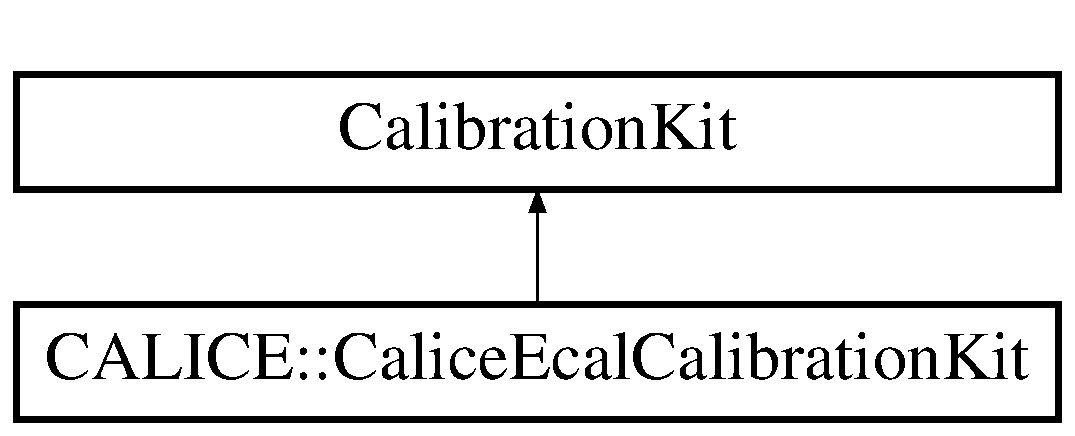
\includegraphics[height=2cm]{classCALICE_1_1CaliceEcalCalibrationKit}
\end{center}
\end{figure}
\subsection*{Public Member Functions}
\begin{DoxyCompactItemize}
\item 
{\bf Calibration} $\ast$ {\bf create} (const std::string \&module\_\-type\_\-col\_\-name, const std::string \&module\_\-calibration\_\-col\_\-name) const 
\begin{DoxyCompactList}\small\item\em create calibration object. \item\end{DoxyCompactList}\end{DoxyCompactItemize}
\subsection*{Static Protected Attributes}
\begin{DoxyCompactItemize}
\item 
static {\bf CaliceEcalCalibrationKit} {\bfseries \_\-\_\-instance}\label{classCALICE_1_1CaliceEcalCalibrationKit_af2b31f371e49d2795d9ae1e3680a4863}

\end{DoxyCompactItemize}


\subsection{Detailed Description}
Create an Calice ECAL calibration object. \begin{DoxySeeAlso}{See also}
\doxyref{CaliceEcalCalibration}{p.}{classCALICE_1_1CaliceEcalCalibration}. 
\end{DoxySeeAlso}


Definition at line 26 of file CaliceEcalCalibration.cc.

\subsection{Member Function Documentation}
\index{CALICE::CaliceEcalCalibrationKit@{CALICE::CaliceEcalCalibrationKit}!create@{create}}
\index{create@{create}!CALICE::CaliceEcalCalibrationKit@{CALICE::CaliceEcalCalibrationKit}}
\subsubsection[{create}]{\setlength{\rightskip}{0pt plus 5cm}{\bf Calibration}$\ast$ CALICE::CaliceEcalCalibrationKit::create (const std::string \& {\em module\_\-type\_\-col\_\-name}, \/  const std::string \& {\em module\_\-calibration\_\-col\_\-name}) const\hspace{0.3cm}{\ttfamily  [inline, virtual]}}\label{classCALICE_1_1CaliceEcalCalibrationKit_aa8754032807fe2e3d7d8dc4225464829}


create calibration object. 
\begin{DoxyParams}{Parameters}
\item[{\em module\_\-type\_\-col\_\-name}]the name of the conditions data collection with the module types. \item[{\em module\_\-calibration\_\-col\_\-name}]the name of the conditions data collection which contains the calibration constants. FIXME: There should be a better method to hand parameters to \doxyref{Calibration}{p.}{classCalibration} objects. \end{DoxyParams}


Implements {\bf CalibrationKit} \doxyref{}{p.}{classCalibrationKit_ab3aea5671d91a7b6f5e839324cf45a70}.

Definition at line 36 of file CaliceEcalCalibration.cc.

The documentation for this class was generated from the following file:\begin{DoxyCompactItemize}
\item 
CaliceEcalCalibration.cc\end{DoxyCompactItemize}

\section{marlin::CaliceTriggerProcessor Class Reference}
\label{classmarlin_1_1CaliceTriggerProcessor}\index{marlin::CaliceTriggerProcessor@{marlin::CaliceTriggerProcessor}}


Class which adds basic trigger information to the event parameters In order to make use of the trigger information this processor has to run $\ast$before$\ast$ each other user defined processor.  


{\ttfamily \#include $<$CaliceTriggerProcessor.hh$>$}\subsection*{Public Member Functions}
\begin{DoxyCompactItemize}
\item 
Processor $\ast$ {\bfseries newProcessor} ()\label{classmarlin_1_1CaliceTriggerProcessor_a8ae7d8ea18ceb4047ebe26f2475e2f3b}

\item 
void {\bfseries init} ()\label{classmarlin_1_1CaliceTriggerProcessor_ad24c5897512a53e0147b25a23276c553}

\item 
void {\bfseries processEvent} (LCEvent $\ast$evt)\label{classmarlin_1_1CaliceTriggerProcessor_a4a2144796b9fb8b27ad713a462545878}

\item 
void {\bfseries end} ()\label{classmarlin_1_1CaliceTriggerProcessor_a75426b0c47cba668cc037e6ca19cd18b}

\end{DoxyCompactItemize}
\subsection*{Private Attributes}
\begin{DoxyCompactItemize}
\item 
std::string {\bf \_\-confTriggerBitsParName}
\begin{DoxyCompactList}\small\item\em par. \item\end{DoxyCompactList}\item 
std::string {\bf \_\-eventTriggerBitsParName}
\begin{DoxyCompactList}\small\item\em par. \item\end{DoxyCompactList}\item 
std::string {\bf \_\-parNameTriggerMainWord}
\begin{DoxyCompactList}\small\item\em Par. \item\end{DoxyCompactList}\item 
std::string {\bf \_\-parNameTriggerPostHistory}
\begin{DoxyCompactList}\small\item\em Par, name of the trigger post history. \item\end{DoxyCompactList}\item 
std::string {\bf \_\-parNameTriggerPreHistory}
\begin{DoxyCompactList}\small\item\em Par, name of the trigger pre history. \item\end{DoxyCompactList}\item 
std::string {\bfseries \_\-parNameTriggerPostHistoryPos}\label{classmarlin_1_1CaliceTriggerProcessor_afc4b7bcc4eb2327e67df20cfedc5b668}

\item 
std::string {\bfseries \_\-parNameTriggerPostHistoryBits}\label{classmarlin_1_1CaliceTriggerProcessor_a06a31c9af414f0539c4504fa54079f67}

\item 
std::string {\bfseries \_\-parNameTriggerPreHistoryPos}\label{classmarlin_1_1CaliceTriggerProcessor_afe63efbbcc0e17aa874778e909240ef4}

\item 
std::string {\bfseries \_\-parNameTriggerPreHistoryBits}\label{classmarlin_1_1CaliceTriggerProcessor_a144777e561189e07ba32fb395de6daf4}

\item 
UInt\_\-t {\bf \_\-noMainWord}
\begin{DoxyCompactList}\small\item\em events for which the main word was not within the valid range. \item\end{DoxyCompactList}\item 
UInt\_\-t {\bf \_\-eventsWithOutOfRangeTriggers}
\begin{DoxyCompactList}\small\item\em events for which possible trigger bits were out of range. \item\end{DoxyCompactList}\item 
StringVec {\bf \_\-beamTriggerNames}
\begin{DoxyCompactList}\small\item\em Names of all trigger which indicated physics events and which will be ignored for pedestal calculation. \item\end{DoxyCompactList}\item 
unsigned int {\bf \_\-beamTriggerBitMask}
\begin{DoxyCompactList}\small\item\em Bit mask of all triggers which indicated physics events and which will be ignored for pedestal calculation. \item\end{DoxyCompactList}\item 
IntVec {\bf \_\-noTriggerActivityRange}
\begin{DoxyCompactList}\small\item\em The time in ns before and after the main word during which there is no beam trigger allowed. \item\end{DoxyCompactList}\end{DoxyCompactItemize}


\subsection{Detailed Description}
Class which adds basic trigger information to the event parameters In order to make use of the trigger information this processor has to run $\ast$before$\ast$ each other user defined processor. It initializes the trigger handler through which the user can obtain more information on trigger issues in other processors. Here it adds the trigger which have fired the event to the event parameters. This trigger information is made persistent with the event and can be later on used in higher level analysis. \begin{DoxyAuthor}{Author}
: R. P�schl DESY 
\end{DoxyAuthor}
\begin{DoxyDate}{Date}
Dec 7 2005 
\end{DoxyDate}


Definition at line 39 of file CaliceTriggerProcessor.hh.

\subsection{Field Documentation}
\index{marlin::CaliceTriggerProcessor@{marlin::CaliceTriggerProcessor}!\_\-beamTriggerBitMask@{\_\-beamTriggerBitMask}}
\index{\_\-beamTriggerBitMask@{\_\-beamTriggerBitMask}!marlin::CaliceTriggerProcessor@{marlin::CaliceTriggerProcessor}}
\subsubsection[{\_\-beamTriggerBitMask}]{\setlength{\rightskip}{0pt plus 5cm}unsigned int {\bf marlin::CaliceTriggerProcessor::\_\-beamTriggerBitMask}\hspace{0.3cm}{\ttfamily  [private]}}\label{classmarlin_1_1CaliceTriggerProcessor_a7bae04321ad0bf2fd8168bfaa2f13f52}


Bit mask of all triggers which indicated physics events and which will be ignored for pedestal calculation. 

Definition at line 65 of file CaliceTriggerProcessor.hh.\index{marlin::CaliceTriggerProcessor@{marlin::CaliceTriggerProcessor}!\_\-beamTriggerNames@{\_\-beamTriggerNames}}
\index{\_\-beamTriggerNames@{\_\-beamTriggerNames}!marlin::CaliceTriggerProcessor@{marlin::CaliceTriggerProcessor}}
\subsubsection[{\_\-beamTriggerNames}]{\setlength{\rightskip}{0pt plus 5cm}StringVec {\bf marlin::CaliceTriggerProcessor::\_\-beamTriggerNames}\hspace{0.3cm}{\ttfamily  [private]}}\label{classmarlin_1_1CaliceTriggerProcessor_ae3443ac3f3dae23e9490552cb270d5f3}


Names of all trigger which indicated physics events and which will be ignored for pedestal calculation. 

Definition at line 64 of file CaliceTriggerProcessor.hh.\index{marlin::CaliceTriggerProcessor@{marlin::CaliceTriggerProcessor}!\_\-confTriggerBitsParName@{\_\-confTriggerBitsParName}}
\index{\_\-confTriggerBitsParName@{\_\-confTriggerBitsParName}!marlin::CaliceTriggerProcessor@{marlin::CaliceTriggerProcessor}}
\subsubsection[{\_\-confTriggerBitsParName}]{\setlength{\rightskip}{0pt plus 5cm}std::string {\bf marlin::CaliceTriggerProcessor::\_\-confTriggerBitsParName}\hspace{0.3cm}{\ttfamily  [private]}}\label{classmarlin_1_1CaliceTriggerProcessor_a71283d68a025529d27f9b59d4939a8ff}


par. name of the configuration trigger bits. 

Definition at line 50 of file CaliceTriggerProcessor.hh.\index{marlin::CaliceTriggerProcessor@{marlin::CaliceTriggerProcessor}!\_\-eventsWithOutOfRangeTriggers@{\_\-eventsWithOutOfRangeTriggers}}
\index{\_\-eventsWithOutOfRangeTriggers@{\_\-eventsWithOutOfRangeTriggers}!marlin::CaliceTriggerProcessor@{marlin::CaliceTriggerProcessor}}
\subsubsection[{\_\-eventsWithOutOfRangeTriggers}]{\setlength{\rightskip}{0pt plus 5cm}UInt\_\-t {\bf marlin::CaliceTriggerProcessor::\_\-eventsWithOutOfRangeTriggers}\hspace{0.3cm}{\ttfamily  [private]}}\label{classmarlin_1_1CaliceTriggerProcessor_a521a453cfb29f46ef79ba17121e89f6f}


events for which possible trigger bits were out of range. 

Definition at line 62 of file CaliceTriggerProcessor.hh.\index{marlin::CaliceTriggerProcessor@{marlin::CaliceTriggerProcessor}!\_\-eventTriggerBitsParName@{\_\-eventTriggerBitsParName}}
\index{\_\-eventTriggerBitsParName@{\_\-eventTriggerBitsParName}!marlin::CaliceTriggerProcessor@{marlin::CaliceTriggerProcessor}}
\subsubsection[{\_\-eventTriggerBitsParName}]{\setlength{\rightskip}{0pt plus 5cm}std::string {\bf marlin::CaliceTriggerProcessor::\_\-eventTriggerBitsParName}\hspace{0.3cm}{\ttfamily  [private]}}\label{classmarlin_1_1CaliceTriggerProcessor_a90f8c6f9aecafda817964a4272c1bc82}


par. name of the event trigger bits. 

Definition at line 51 of file CaliceTriggerProcessor.hh.\index{marlin::CaliceTriggerProcessor@{marlin::CaliceTriggerProcessor}!\_\-noMainWord@{\_\-noMainWord}}
\index{\_\-noMainWord@{\_\-noMainWord}!marlin::CaliceTriggerProcessor@{marlin::CaliceTriggerProcessor}}
\subsubsection[{\_\-noMainWord}]{\setlength{\rightskip}{0pt plus 5cm}UInt\_\-t {\bf marlin::CaliceTriggerProcessor::\_\-noMainWord}\hspace{0.3cm}{\ttfamily  [private]}}\label{classmarlin_1_1CaliceTriggerProcessor_a08d5438ca77dc832d115d7f3f73dba59}


events for which the main word was not within the valid range. 

Definition at line 61 of file CaliceTriggerProcessor.hh.\index{marlin::CaliceTriggerProcessor@{marlin::CaliceTriggerProcessor}!\_\-noTriggerActivityRange@{\_\-noTriggerActivityRange}}
\index{\_\-noTriggerActivityRange@{\_\-noTriggerActivityRange}!marlin::CaliceTriggerProcessor@{marlin::CaliceTriggerProcessor}}
\subsubsection[{\_\-noTriggerActivityRange}]{\setlength{\rightskip}{0pt plus 5cm}IntVec {\bf marlin::CaliceTriggerProcessor::\_\-noTriggerActivityRange}\hspace{0.3cm}{\ttfamily  [private]}}\label{classmarlin_1_1CaliceTriggerProcessor_ab54172955bbe9099625b548046dd79ea}


The time in ns before and after the main word during which there is no beam trigger allowed. 

Definition at line 66 of file CaliceTriggerProcessor.hh.\index{marlin::CaliceTriggerProcessor@{marlin::CaliceTriggerProcessor}!\_\-parNameTriggerMainWord@{\_\-parNameTriggerMainWord}}
\index{\_\-parNameTriggerMainWord@{\_\-parNameTriggerMainWord}!marlin::CaliceTriggerProcessor@{marlin::CaliceTriggerProcessor}}
\subsubsection[{\_\-parNameTriggerMainWord}]{\setlength{\rightskip}{0pt plus 5cm}std::string {\bf marlin::CaliceTriggerProcessor::\_\-parNameTriggerMainWord}\hspace{0.3cm}{\ttfamily  [private]}}\label{classmarlin_1_1CaliceTriggerProcessor_a7c9c1511a3be17e49f6f416bea095eb4}


Par. name of the trigger main word. 

Definition at line 52 of file CaliceTriggerProcessor.hh.\index{marlin::CaliceTriggerProcessor@{marlin::CaliceTriggerProcessor}!\_\-parNameTriggerPostHistory@{\_\-parNameTriggerPostHistory}}
\index{\_\-parNameTriggerPostHistory@{\_\-parNameTriggerPostHistory}!marlin::CaliceTriggerProcessor@{marlin::CaliceTriggerProcessor}}
\subsubsection[{\_\-parNameTriggerPostHistory}]{\setlength{\rightskip}{0pt plus 5cm}std::string {\bf marlin::CaliceTriggerProcessor::\_\-parNameTriggerPostHistory}\hspace{0.3cm}{\ttfamily  [private]}}\label{classmarlin_1_1CaliceTriggerProcessor_a6a1a2c84f826a0c56c5475c4ca79794b}


Par, name of the trigger post history. 

Definition at line 53 of file CaliceTriggerProcessor.hh.\index{marlin::CaliceTriggerProcessor@{marlin::CaliceTriggerProcessor}!\_\-parNameTriggerPreHistory@{\_\-parNameTriggerPreHistory}}
\index{\_\-parNameTriggerPreHistory@{\_\-parNameTriggerPreHistory}!marlin::CaliceTriggerProcessor@{marlin::CaliceTriggerProcessor}}
\subsubsection[{\_\-parNameTriggerPreHistory}]{\setlength{\rightskip}{0pt plus 5cm}std::string {\bf marlin::CaliceTriggerProcessor::\_\-parNameTriggerPreHistory}\hspace{0.3cm}{\ttfamily  [private]}}\label{classmarlin_1_1CaliceTriggerProcessor_af679233aa39405f79cf03d326cd5ec95}


Par, name of the trigger pre history. 

Definition at line 54 of file CaliceTriggerProcessor.hh.

The documentation for this class was generated from the following files:\begin{DoxyCompactItemize}
\item 
CaliceTriggerProcessor.hh\item 
CaliceTriggerProcessor.cc\end{DoxyCompactItemize}

\section{CALICE::CellPar\_\-t Class Reference}
\label{classCALICE_1_1CellPar__t}\index{CALICE::CellPar\_\-t@{CALICE::CellPar\_\-t}}
\subsection*{Public Member Functions}
\begin{DoxyCompactItemize}
\item 
{\bfseries CellPar\_\-t} (float x, float y, unsigned int index)\label{classCALICE_1_1CellPar__t_a4a421af43e94b139ef5dcfd7525c2271}

\item 
unsigned int {\bfseries index} () const \label{classCALICE_1_1CellPar__t_a24feee6789d715f0503092d8594b34e4}

\item 
const float \& {\bfseries posX} () const \label{classCALICE_1_1CellPar__t_a1e053bcf09cd9d47c42f5bb05e18bb10}

\item 
const float \& {\bfseries posY} () const \label{classCALICE_1_1CellPar__t_a64b678b384ef3bc481ce1c2f9aa07808}

\end{DoxyCompactItemize}
\subsection*{Data Fields}
\begin{DoxyCompactItemize}
\item 
unsigned int {\bfseries \_\-index}\label{classCALICE_1_1CellPar__t_a2f58580b68327c8eab7867461106119a}

\item 
float {\bfseries \_\-posX}\label{classCALICE_1_1CellPar__t_a3b93d132cf7bb73e042c88c060c8e115}

\item 
float {\bfseries \_\-posY}\label{classCALICE_1_1CellPar__t_a43eb3039ef1edbedba6953629cd16c05}

\end{DoxyCompactItemize}


\subsection{Detailed Description}


Definition at line 101 of file VRawADCValueProcessor.cc.

The documentation for this class was generated from the following file:\begin{DoxyCompactItemize}
\item 
VRawADCValueProcessor.cc\end{DoxyCompactItemize}

\section{CALICE::CellParameter Class Reference}
\label{classCALICE_1_1CellParameter}\index{CALICE::CellParameter@{CALICE::CellParameter}}


Information about a pad: Pedestal, noise, etc.  


{\ttfamily \#include $<$CellParameter.hh$>$}\subsection*{Public Member Functions}
\begin{DoxyCompactItemize}
\item 
{\bf CellParameter} (LCObject $\ast$obj)\label{classCALICE_1_1CellParameter_a3dbf58dc25acfd28b79bde1793d97cbe}

\begin{DoxyCompactList}\small\item\em 'Copy constructor' needed to interpret LCCollection read from file/database. \item\end{DoxyCompactList}\item 
void {\bf resetSums} ()
\begin{DoxyCompactList}\small\item\em Reset the sums which are used to calculate the pedestals and the noise. \item\end{DoxyCompactList}\item 
void {\bfseries resetSaturationCounter} ()\label{classCALICE_1_1CellParameter_a899306ee8d7c50c7b4f674826384088f}

\item 
void {\bfseries resetHitCounter} ()\label{classCALICE_1_1CellParameter_a96068c40f7efdc6f8065998405f00ca3}

\item 
void {\bfseries resetAll} ()\label{classCALICE_1_1CellParameter_ac296a0d601c33323999152ee709a1abf}

\item 
void {\bf setSum} (Float\_\-t a\_\-sum)
\begin{DoxyCompactList}\small\item\em Set the sum of the adc values (used to calculate the pedestal). \item\end{DoxyCompactList}\item 
Float\_\-t {\bf getSum} () const 
\begin{DoxyCompactList}\small\item\em Get the sum of the adc values (used to calculate the pedestal). \item\end{DoxyCompactList}\item 
void {\bf setSum2} (Float\_\-t a\_\-sum2)
\begin{DoxyCompactList}\small\item\em Set the sum of the adc values squared (used to calculate the noise). \item\end{DoxyCompactList}\item 
Float\_\-t {\bf getSum2} () const 
\begin{DoxyCompactList}\small\item\em Get the sum of the adc values squared (used to calculate the noise). \item\end{DoxyCompactList}\item 
void {\bf setNValues} (UInt\_\-t n\_\-values)\label{classCALICE_1_1CellParameter_acd7683bda27b9dc1a3b9bf9dd67fdc69}

\begin{DoxyCompactList}\small\item\em Set the number of values added to the sums. \item\end{DoxyCompactList}\item 
UInt\_\-t {\bf getNValues} () const \label{classCALICE_1_1CellParameter_a9d83d4f709324d0bbdd464c54aa1a39c}

\begin{DoxyCompactList}\small\item\em Get the number of values added to the sums. \item\end{DoxyCompactList}\item 
void {\bf setPedestal} (Float\_\-t a\_\-pedestal)\label{classCALICE_1_1CellParameter_af3c9c24f740b0822c4b996a363507cf5}

\begin{DoxyCompactList}\small\item\em Set the pedestal. \item\end{DoxyCompactList}\item 
Float\_\-t {\bf getPedestal} () const 
\begin{DoxyCompactList}\small\item\em Get the pedestal. \item\end{DoxyCompactList}\item 
void {\bf setOldPedestal} (Float\_\-t an\_\-old\_\-pedestal)
\begin{DoxyCompactList}\small\item\em Set the old pedestal. \item\end{DoxyCompactList}\item 
Float\_\-t {\bf getOldPedestal} () const 
\begin{DoxyCompactList}\small\item\em Get the old pedestal The result is undefined before the pedestals and the noise have been adjusted or calculated. \item\end{DoxyCompactList}\item 
void {\bf setNoise} (Float\_\-t a\_\-noise)\label{classCALICE_1_1CellParameter_a4ecc22743f2049d0558d6d625038907d}

\begin{DoxyCompactList}\small\item\em Set the noise. \item\end{DoxyCompactList}\item 
Float\_\-t {\bf getNoise} () const 
\begin{DoxyCompactList}\small\item\em Get the noise. \item\end{DoxyCompactList}\item 
void {\bf setOldNoise} (Float\_\-t an\_\-old\_\-noise)
\begin{DoxyCompactList}\small\item\em Set the old noise. \item\end{DoxyCompactList}\item 
Float\_\-t {\bf getOldNoise} () const 
\begin{DoxyCompactList}\small\item\em Get the old noise. \item\end{DoxyCompactList}\item 
void {\bf setMaxValue} (Float\_\-t a\_\-max\_\-value)
\begin{DoxyCompactList}\small\item\em set the maximum value for a cell ({\bfseries shares storage with pedestal}). \item\end{DoxyCompactList}\item 
Float\_\-t {\bf getMaxValue} () const \label{classCALICE_1_1CellParameter_af1a12f740874cc83f5e35ba5d8d0eefd}

\begin{DoxyCompactList}\small\item\em get the maximum value of a cell (shares storage with pedestal) This function only returns the expected result before pedestals/noise are calculated. \item\end{DoxyCompactList}\item 
void {\bf add} (Float\_\-t adc)
\begin{DoxyCompactList}\small\item\em Build sums used to calculate pedestals and noise. \item\end{DoxyCompactList}\item 
void {\bf sub} (Float\_\-t adc)
\begin{DoxyCompactList}\small\item\em Subtract a previously added adc value from the sums to return to the prior condition. \item\end{DoxyCompactList}\item 
void {\bf calculate} ()\label{classCALICE_1_1CellParameter_a0548e12eab1fdba4da79dee09bc18aee}

\begin{DoxyCompactList}\small\item\em Caluclate the pedestal and the noise from the sums. \item\end{DoxyCompactList}\item 
void {\bf adjustPedestalNoise} (Float\_\-t adc, UInt\_\-t keep\_\-n\_\-minus\_\-one)
\begin{DoxyCompactList}\small\item\em Adjust the pedestal and the noise using the new ADC value. \item\end{DoxyCompactList}\item 
Bool\_\-t {\bf isDead} () const \label{classCALICE_1_1CellParameter_ab1ae07641b9b6d188cfc8aa7b6641e0a}

\begin{DoxyCompactList}\small\item\em Return kTRUE if the pad is considered to be dead. \item\end{DoxyCompactList}\item 
void {\bf setDead} (Bool\_\-t is\_\-dead=true)
\begin{DoxyCompactList}\small\item\em Declare the pad to be dead (or revive pad (is\_\-dead=kFALSE). \item\end{DoxyCompactList}\item 
UInt\_\-t {\bf getSaturationCounter} () const 
\begin{DoxyCompactList}\small\item\em Get the value of the saturation counter. \item\end{DoxyCompactList}\item 
void {\bf incrementSaturationCounter} ()
\begin{DoxyCompactList}\small\item\em Increment the saturation counter. \item\end{DoxyCompactList}\item 
UInt\_\-t {\bf getNHits} () const 
\begin{DoxyCompactList}\small\item\em Get the number of hits. \item\end{DoxyCompactList}\item 
void {\bf incrementNHits} ()
\begin{DoxyCompactList}\small\item\em Increment the hit counter. \item\end{DoxyCompactList}\item 
Float\_\-t {\bf getNHitsFloat} () const 
\begin{DoxyCompactList}\small\item\em Function which returns the number of hits converted into a float. \item\end{DoxyCompactList}\item 
void {\bf initADCMemory} ()
\begin{DoxyCompactList}\small\item\em Initialse the array which memorises the last pedestal subtracted values. \item\end{DoxyCompactList}\item 
void {\bf setADCMemoryValue} (UInt\_\-t memory\_\-cell\_\-i, Float\_\-t an\_\-adc\_\-value)\label{classCALICE_1_1CellParameter_a2150862e4495b17184abcad51b85d67d}

\begin{DoxyCompactList}\small\item\em Memorise an ADC value in the given cell. \item\end{DoxyCompactList}\item 
Float\_\-t {\bf getADCMemoryValue} (UInt\_\-t memory\_\-cell\_\-i) const \label{classCALICE_1_1CellParameter_a64123c38f4b0fb4e0c519d2c144d89db}

\begin{DoxyCompactList}\small\item\em Get a memorised ADC value from the given cell. \item\end{DoxyCompactList}\item 
void {\bf setADCMemoryWritePos} (UInt\_\-t memory\_\-cell\_\-i)\label{classCALICE_1_1CellParameter_a6d667e7086d288b9797ea58407ab6eba}

\begin{DoxyCompactList}\small\item\em Set the current ADC memory cell. \item\end{DoxyCompactList}\item 
void {\bfseries setNextADCMemory} ()\label{classCALICE_1_1CellParameter_acd3539f67f1b47ebdd719e0393788b94}

\item 
Float\_\-t {\bf getADCMemoryValue} () const \label{classCALICE_1_1CellParameter_a6d46c4d193e8d3bda70f0f6f8a350ef9}

\begin{DoxyCompactList}\small\item\em Get a memorised ADC value. \item\end{DoxyCompactList}\item 
void {\bf setADCMemoryValue} (Float\_\-t pedestal\_\-subtracted\_\-value)
\begin{DoxyCompactList}\small\item\em Memorise an ADC value. \item\end{DoxyCompactList}\item 
Float\_\-t {\bf getMeanADCValue} (Float\_\-t pedestal\_\-subtracted\_\-value)
\begin{DoxyCompactList}\small\item\em Get the mean value of a group of pedestal subtracted ADC values (the maximum is removed). \item\end{DoxyCompactList}\item 
void {\bf shiftPedestal} (Float\_\-t shift)
\begin{DoxyCompactList}\small\item\em Shift the current and the old pedestal by this value. \item\end{DoxyCompactList}\item 
UInt\_\-t {\bf getNPedestalChanges} () const 
\begin{DoxyCompactList}\small\item\em Get the value of the pedestal change counter. \item\end{DoxyCompactList}\item 
const std::string {\bf getTypeName} () const \label{classCALICE_1_1CellParameter_add6643930ab5dcb3ff15c8a0aeeb65a4}

\begin{DoxyCompactList}\small\item\em Return the type of the class. \item\end{DoxyCompactList}\item 
const std::string {\bf getDataDescription} () const \label{classCALICE_1_1CellParameter_a510675057c37ce93c7f992257c9cc8bb}

\begin{DoxyCompactList}\small\item\em Return a brief description of the data members. \item\end{DoxyCompactList}\end{DoxyCompactItemize}
\subsection*{Protected Member Functions}
\begin{DoxyCompactItemize}
\item 
void {\bf setSaturationCounter} (UInt\_\-t saturation)
\begin{DoxyCompactList}\small\item\em Set the value of the saturation counter. \item\end{DoxyCompactList}\item 
void {\bf setNHits} (UInt\_\-t n\_\-hits)
\begin{DoxyCompactList}\small\item\em Set the value of the hit counter. \item\end{DoxyCompactList}\item 
void {\bf setNPedestalChanges} (UInt\_\-t n\_\-pedestal\_\-changes)
\begin{DoxyCompactList}\small\item\em Set the value of the pedestal change counter. \item\end{DoxyCompactList}\item 
void {\bf incrementNPedestalChanges} ()
\begin{DoxyCompactList}\small\item\em Increment the pedestal change counter. \item\end{DoxyCompactList}\end{DoxyCompactItemize}


\subsection{Detailed Description}
Information about a pad: Pedestal, noise, etc. This class hold the pedestal, the noise, the number of accumulated hits, a saturation counter and a flag which indicates whether the pad is considered to be dead. 

Definition at line 70 of file CellParameter.hh.

\subsection{Member Function Documentation}
\index{CALICE::CellParameter@{CALICE::CellParameter}!add@{add}}
\index{add@{add}!CALICE::CellParameter@{CALICE::CellParameter}}
\subsubsection[{add}]{\setlength{\rightskip}{0pt plus 5cm}void CALICE::CellParameter::add (Float\_\-t {\em adc})\hspace{0.3cm}{\ttfamily  [inline]}}\label{classCALICE_1_1CellParameter_a199f221d2988995dedbb75b9be43e9ab}


Build sums used to calculate pedestals and noise. The storage for the old pedestals and noise is abused to store the sums \begin{DoxySeeAlso}{See also}
\doxyref{CellParameter::sub}{p.}{classCALICE_1_1CellParameter_a09cb9e322c9b22d1591244eaa1ded505} 
\end{DoxySeeAlso}


Definition at line 190 of file CellParameter.hh.

Referenced by CALICE::SimpleHitSearch::accumulateEventsForInitialPedestalNoiseCalculation(), CALICE::SimpleHitSearch::accumulateEventsForPedestalNoiseCalculationWithHitRejection(), and CALICE::SimpleHitSearch::accumulateEventsForPedestalNoiseCalculationWithHitRejectionAndPedestalShiftDetection().\index{CALICE::CellParameter@{CALICE::CellParameter}!adjustPedestalNoise@{adjustPedestalNoise}}
\index{adjustPedestalNoise@{adjustPedestalNoise}!CALICE::CellParameter@{CALICE::CellParameter}}
\subsubsection[{adjustPedestalNoise}]{\setlength{\rightskip}{0pt plus 5cm}void CALICE::CellParameter::adjustPedestalNoise (Float\_\-t {\em adc}, \/  UInt\_\-t {\em keep\_\-n\_\-minus\_\-one})\hspace{0.3cm}{\ttfamily  [inline]}}\label{classCALICE_1_1CellParameter_a15bfbaa4918ac7d9aaf841c0483a8a19}


Adjust the pedestal and the noise using the new ADC value. 
\begin{DoxyParams}{Parameters}
\item[{\em adc}]the new ADC value \item[{\em keep\_\-n\_\-minus\_\-one}]the current pedestal and noise are given a weight of this value + 1 and the new ADC value get the weight 1\end{DoxyParams}
The current pedestal and the current noise are memorised (\doxyref{getPedestal}{p.}{classCALICE_1_1CellParameter_a3223608e5f680b674e7181b5c4495935} and \doxyref{getNoise}{p.}{classCALICE_1_1CellParameter_a58d1f99e4ef0452b94fef27d5de1cc1e}) and then they are updated. 

Definition at line 230 of file CellParameter.hh.

References getNoise(), getPedestal(), setNoise(), setOldNoise(), setOldPedestal(), and setPedestal().

Referenced by CALICE::SimpleHitSearch::searchHitsAndAdjustPedestalsAndNoise().\index{CALICE::CellParameter@{CALICE::CellParameter}!getMeanADCValue@{getMeanADCValue}}
\index{getMeanADCValue@{getMeanADCValue}!CALICE::CellParameter@{CALICE::CellParameter}}
\subsubsection[{getMeanADCValue}]{\setlength{\rightskip}{0pt plus 5cm}Float\_\-t CALICE::CellParameter::getMeanADCValue (Float\_\-t {\em pedestal\_\-subtracted\_\-value})\hspace{0.3cm}{\ttfamily  [inline]}}\label{classCALICE_1_1CellParameter_a70a20f2d63910738f6d725fd5db83d4f}


Get the mean value of a group of pedestal subtracted ADC values (the maximum is removed). The mean value is used to track jumps in the pedestal. If the jump is larger than a certain threshold the pedestal is considered to have changed. 

Definition at line 387 of file CellParameter.hh.

References getADCMemoryValue(), and setADCMemoryValue().

Referenced by CALICE::SimpleHitSearch::accumulateEventsForPedestalNoiseCalculationWithHitRejectionAndPedestalShiftDetection().\index{CALICE::CellParameter@{CALICE::CellParameter}!getNHits@{getNHits}}
\index{getNHits@{getNHits}!CALICE::CellParameter@{CALICE::CellParameter}}
\subsubsection[{getNHits}]{\setlength{\rightskip}{0pt plus 5cm}UInt\_\-t CALICE::CellParameter::getNHits () const\hspace{0.3cm}{\ttfamily  [inline]}}\label{classCALICE_1_1CellParameter_aaeb9e38b31539b337be9e7b0522005ef}


Get the number of hits. The hit counter is increased when ever the pedestal subtracted ADC value is above a signal or signal-\/to-\/noise threshold. 

Definition at line 291 of file CellParameter.hh.

Referenced by getNHitsFloat(), and incrementNHits().\index{CALICE::CellParameter@{CALICE::CellParameter}!getNHitsFloat@{getNHitsFloat}}
\index{getNHitsFloat@{getNHitsFloat}!CALICE::CellParameter@{CALICE::CellParameter}}
\subsubsection[{getNHitsFloat}]{\setlength{\rightskip}{0pt plus 5cm}Float\_\-t CALICE::CellParameter::getNHitsFloat () const\hspace{0.3cm}{\ttfamily  [inline]}}\label{classCALICE_1_1CellParameter_a32aaee7ca8e819dae916272e109171f5}


Function which returns the number of hits converted into a float. This function can be used together with getNoise and getPedestal in a generic way (e.g. typedef Float\_\-t \doxyref{CellParameter}{p.}{classCALICE_1_1CellParameter}::$\ast$GetFloatFunc\_\-t();) 

Definition at line 302 of file CellParameter.hh.

References getNHits().\index{CALICE::CellParameter@{CALICE::CellParameter}!getNoise@{getNoise}}
\index{getNoise@{getNoise}!CALICE::CellParameter@{CALICE::CellParameter}}
\subsubsection[{getNoise}]{\setlength{\rightskip}{0pt plus 5cm}Float\_\-t CALICE::CellParameter::getNoise () const\hspace{0.3cm}{\ttfamily  [inline]}}\label{classCALICE_1_1CellParameter_a58d1f99e4ef0452b94fef27d5de1cc1e}


Get the noise. The result is undefined before the pedestals and the noise are calculated. 

Definition at line 153 of file CellParameter.hh.

Referenced by CALICE::SimpleHitSearch::accumulateEventsForPedestalNoiseCalculationWithHitRejection(), CALICE::SimpleHitSearch::accumulateEventsForPedestalNoiseCalculationWithHitRejectionAndPedestalShiftDetection(), adjustPedestalNoise(), CALICE::SimpleHitSearch::calculatePedestalNoiseAndDeclareCellsDead(), CALICE::PedestalNoiseHistograms::processEvent(), CALICE::AverageHistoryGraphs::processEvent(), CALICE::SimpleHitSearch::searchHits(), CALICE::SimpleHitSearch::searchHitsAndAdjustPedestalsAndNoise(), and CALICE::SimpleHitSearch::showNoiseStat().\index{CALICE::CellParameter@{CALICE::CellParameter}!getNPedestalChanges@{getNPedestalChanges}}
\index{getNPedestalChanges@{getNPedestalChanges}!CALICE::CellParameter@{CALICE::CellParameter}}
\subsubsection[{getNPedestalChanges}]{\setlength{\rightskip}{0pt plus 5cm}UInt\_\-t CALICE::CellParameter::getNPedestalChanges () const\hspace{0.3cm}{\ttfamily  [inline]}}\label{classCALICE_1_1CellParameter_a8f6f313321e39c27dc7f09899aa6e948}


Get the value of the pedestal change counter. The PedestalChange counter is increased when ever the ADC value is outside of a certain range 

Definition at line 425 of file CellParameter.hh.

Referenced by incrementNPedestalChanges().\index{CALICE::CellParameter@{CALICE::CellParameter}!getOldNoise@{getOldNoise}}
\index{getOldNoise@{getOldNoise}!CALICE::CellParameter@{CALICE::CellParameter}}
\subsubsection[{getOldNoise}]{\setlength{\rightskip}{0pt plus 5cm}Float\_\-t CALICE::CellParameter::getOldNoise () const\hspace{0.3cm}{\ttfamily  [inline]}}\label{classCALICE_1_1CellParameter_a3bfb3c568c64aee79f779c649b941dc7}


Get the old noise. The result is undefined before the pedestals and the noise have been adjusted or calculated. In the latter case the old and the \char`\"{}new\char`\"{} noise are the same. 

Definition at line 164 of file CellParameter.hh.

Referenced by CALICE::SimpleHitSearch::searchHitsAndAdjustPedestalsAndNoise(), and CALICE::SimpleHitSearch::showCurrentNoiseStat().\index{CALICE::CellParameter@{CALICE::CellParameter}!getOldPedestal@{getOldPedestal}}
\index{getOldPedestal@{getOldPedestal}!CALICE::CellParameter@{CALICE::CellParameter}}
\subsubsection[{getOldPedestal}]{\setlength{\rightskip}{0pt plus 5cm}Float\_\-t CALICE::CellParameter::getOldPedestal () const\hspace{0.3cm}{\ttfamily  [inline]}}\label{classCALICE_1_1CellParameter_ac159d4054fd122bfb2fb6c6730110126}


Get the old pedestal The result is undefined before the pedestals and the noise have been adjusted or calculated. In the latter case the old and the \char`\"{}new\char`\"{} pedestals are the same. 

Definition at line 143 of file CellParameter.hh.

Referenced by CALICE::SimpleHitSearch::searchHitsAndAdjustPedestalsAndNoise(), shiftPedestal(), and CALICE::SimpleHitSearch::showCurrentNoiseStat().\index{CALICE::CellParameter@{CALICE::CellParameter}!getPedestal@{getPedestal}}
\index{getPedestal@{getPedestal}!CALICE::CellParameter@{CALICE::CellParameter}}
\subsubsection[{getPedestal}]{\setlength{\rightskip}{0pt plus 5cm}Float\_\-t CALICE::CellParameter::getPedestal () const\hspace{0.3cm}{\ttfamily  [inline]}}\label{classCALICE_1_1CellParameter_a3223608e5f680b674e7181b5c4495935}


Get the pedestal. The result is undefined before the pedestals and the noise are calculated. 

Definition at line 131 of file CellParameter.hh.

Referenced by CALICE::SimpleHitSearch::accumulateEventsForPedestalNoiseCalculationWithHitRejection(), CALICE::SimpleHitSearch::accumulateEventsForPedestalNoiseCalculationWithHitRejectionAndPedestalShiftDetection(), adjustPedestalNoise(), CALICE::SimpleHitSearch::calculatePedestalNoiseAndDeclareCellsDead(), initADCMemory(), CALICE::PedestalNoiseHistograms::processEvent(), CALICE::AverageHistoryGraphs::processEvent(), CALICE::SimpleHitSearch::searchHits(), CALICE::SimpleHitSearch::searchHitsAndAdjustPedestalsAndNoise(), shiftPedestal(), and CALICE::SimpleHitSearch::showNoiseStat().\index{CALICE::CellParameter@{CALICE::CellParameter}!getSaturationCounter@{getSaturationCounter}}
\index{getSaturationCounter@{getSaturationCounter}!CALICE::CellParameter@{CALICE::CellParameter}}
\subsubsection[{getSaturationCounter}]{\setlength{\rightskip}{0pt plus 5cm}UInt\_\-t CALICE::CellParameter::getSaturationCounter () const\hspace{0.3cm}{\ttfamily  [inline]}}\label{classCALICE_1_1CellParameter_ae4ef4a080c6400a667dd37dd7ce853fd}


Get the value of the saturation counter. The saturation counter is increased when ever the ADC value is outside of a certain range. The saturation counter is used to mark cells as dead. Thus, it must not be incremented if a cell is dead. 

Definition at line 274 of file CellParameter.hh.

Referenced by CALICE::SimpleHitSearch::calculatePedestalNoiseAndDeclareCellsDead(), incrementSaturationCounter(), and isDead().\index{CALICE::CellParameter@{CALICE::CellParameter}!getSum@{getSum}}
\index{getSum@{getSum}!CALICE::CellParameter@{CALICE::CellParameter}}
\subsubsection[{getSum}]{\setlength{\rightskip}{0pt plus 5cm}Float\_\-t CALICE::CellParameter::getSum () const\hspace{0.3cm}{\ttfamily  [inline]}}\label{classCALICE_1_1CellParameter_afa7c61c8a0fd6f4b93d5113c2ee30285}


Get the sum of the adc values (used to calculate the pedestal). The result is undefined after the noise and the pedestals have been calculated. 

Definition at line 101 of file CellParameter.hh.

Referenced by calculate().\index{CALICE::CellParameter@{CALICE::CellParameter}!getSum2@{getSum2}}
\index{getSum2@{getSum2}!CALICE::CellParameter@{CALICE::CellParameter}}
\subsubsection[{getSum2}]{\setlength{\rightskip}{0pt plus 5cm}Float\_\-t CALICE::CellParameter::getSum2 () const\hspace{0.3cm}{\ttfamily  [inline]}}\label{classCALICE_1_1CellParameter_ac509a47a088106a0fbd2fc2fc17dcca0}


Get the sum of the adc values squared (used to calculate the noise). The result is undefined after the noise and the pedestals have been calculated. 

Definition at line 112 of file CellParameter.hh.

Referenced by calculate().\index{CALICE::CellParameter@{CALICE::CellParameter}!incrementNHits@{incrementNHits}}
\index{incrementNHits@{incrementNHits}!CALICE::CellParameter@{CALICE::CellParameter}}
\subsubsection[{incrementNHits}]{\setlength{\rightskip}{0pt plus 5cm}void CALICE::CellParameter::incrementNHits ()\hspace{0.3cm}{\ttfamily  [inline]}}\label{classCALICE_1_1CellParameter_ab44ebb0a1c9e33f0fd4dcf7796b6c3de}


Increment the hit counter. The hit counter is increased when ever the ADC value is outside of a certain range 

Definition at line 296 of file CellParameter.hh.

References getNHits(), and setNHits().

Referenced by CALICE::SimpleHitSearch::searchHits(), and CALICE::SimpleHitSearch::searchHitsAndAdjustPedestalsAndNoise().\index{CALICE::CellParameter@{CALICE::CellParameter}!incrementNPedestalChanges@{incrementNPedestalChanges}}
\index{incrementNPedestalChanges@{incrementNPedestalChanges}!CALICE::CellParameter@{CALICE::CellParameter}}
\subsubsection[{incrementNPedestalChanges}]{\setlength{\rightskip}{0pt plus 5cm}void CALICE::CellParameter::incrementNPedestalChanges ()\hspace{0.3cm}{\ttfamily  [inline, protected]}}\label{classCALICE_1_1CellParameter_a6c7c08f561c2581f43be8003f2a0312b}


Increment the pedestal change counter. The PedestalChange counter is increased when ever the ADC value is outside of a certain range 

Definition at line 431 of file CellParameter.hh.

References getNPedestalChanges(), and setNPedestalChanges().

Referenced by shiftPedestal().\index{CALICE::CellParameter@{CALICE::CellParameter}!incrementSaturationCounter@{incrementSaturationCounter}}
\index{incrementSaturationCounter@{incrementSaturationCounter}!CALICE::CellParameter@{CALICE::CellParameter}}
\subsubsection[{incrementSaturationCounter}]{\setlength{\rightskip}{0pt plus 5cm}void CALICE::CellParameter::incrementSaturationCounter ()\hspace{0.3cm}{\ttfamily  [inline]}}\label{classCALICE_1_1CellParameter_a79423a46a99deb6623624f7974f414b1}


Increment the saturation counter. The saturation counter is increased when ever the ADC value is outside of a certain range 

Definition at line 279 of file CellParameter.hh.

References getSaturationCounter(), and setSaturationCounter().

Referenced by CALICE::SimpleHitSearch::accumulateEventsForInitialPedestalNoiseCalculation(), CALICE::SimpleHitSearch::accumulateEventsForPedestalNoiseCalculationWithHitRejection(), CALICE::SimpleHitSearch::accumulateEventsForPedestalNoiseCalculationWithHitRejectionAndPedestalShiftDetection(), CALICE::SimpleHitSearch::searchHits(), and CALICE::SimpleHitSearch::searchHitsAndAdjustPedestalsAndNoise().\index{CALICE::CellParameter@{CALICE::CellParameter}!initADCMemory@{initADCMemory}}
\index{initADCMemory@{initADCMemory}!CALICE::CellParameter@{CALICE::CellParameter}}
\subsubsection[{initADCMemory}]{\setlength{\rightskip}{0pt plus 5cm}void CALICE::CellParameter::initADCMemory ()\hspace{0.3cm}{\ttfamily  [inline]}}\label{classCALICE_1_1CellParameter_ad5b4b06d0eb86e98c21d9119fc3a8d30}


Initialse the array which memorises the last pedestal subtracted values. \begin{Desc}
\item[{\bf Todo}]initialsie with pedestal or zero? \end{Desc}


Definition at line 308 of file CellParameter.hh.

References getPedestal(), and setADCMemoryValue().\index{CALICE::CellParameter@{CALICE::CellParameter}!resetSums@{resetSums}}
\index{resetSums@{resetSums}!CALICE::CellParameter@{CALICE::CellParameter}}
\subsubsection[{resetSums}]{\setlength{\rightskip}{0pt plus 5cm}void CALICE::CellParameter::resetSums ()\hspace{0.3cm}{\ttfamily  [inline]}}\label{classCALICE_1_1CellParameter_a6a81bd8e46ad7e4fb8df9847ca4397a5}


Reset the sums which are used to calculate the pedestals and the noise. This function should be called before ADC values are accumulated and added with \doxyref{add}{p.}{classCALICE_1_1CellParameter_a199f221d2988995dedbb75b9be43e9ab} to the sums. 

Definition at line 86 of file CellParameter.hh.

References setNValues(), setSum(), and setSum2().\index{CALICE::CellParameter@{CALICE::CellParameter}!setADCMemoryValue@{setADCMemoryValue}}
\index{setADCMemoryValue@{setADCMemoryValue}!CALICE::CellParameter@{CALICE::CellParameter}}
\subsubsection[{setADCMemoryValue}]{\setlength{\rightskip}{0pt plus 5cm}void CALICE::CellParameter::setADCMemoryValue (Float\_\-t {\em pedestal\_\-subtracted\_\-value})\hspace{0.3cm}{\ttfamily  [inline]}}\label{classCALICE_1_1CellParameter_aea4348d37ee17df1cec6c4a2e8c38217}


Memorise an ADC value. The given pedestal subtracted ADC value is memorised at the current write postion and the position counter is advanced. 

Definition at line 379 of file CellParameter.hh.\index{CALICE::CellParameter@{CALICE::CellParameter}!setDead@{setDead}}
\index{setDead@{setDead}!CALICE::CellParameter@{CALICE::CellParameter}}
\subsubsection[{setDead}]{\setlength{\rightskip}{0pt plus 5cm}void CALICE::CellParameter::setDead (Bool\_\-t {\em is\_\-dead} = {\ttfamily true})\hspace{0.3cm}{\ttfamily  [inline]}}\label{classCALICE_1_1CellParameter_a0ad31de9b53fc6ebed4c7be6a53e7a57}


Declare the pad to be dead (or revive pad (is\_\-dead=kFALSE). The status whether a pad is dead is stored in the saturation counter. Thus, a reviving a cell will reset the saturation counter to zero. 

Definition at line 260 of file CellParameter.hh.

References setSaturationCounter().

Referenced by CALICE::SimpleHitSearch::calculatePedestalNoiseAndDeclareCellsDead().\index{CALICE::CellParameter@{CALICE::CellParameter}!setMaxValue@{setMaxValue}}
\index{setMaxValue@{setMaxValue}!CALICE::CellParameter@{CALICE::CellParameter}}
\subsubsection[{setMaxValue}]{\setlength{\rightskip}{0pt plus 5cm}void CALICE::CellParameter::setMaxValue (Float\_\-t {\em a\_\-max\_\-value})\hspace{0.3cm}{\ttfamily  [inline]}}\label{classCALICE_1_1CellParameter_add7570a3502df326aa422603be276c8a}


set the maximum value for a cell ({\bfseries shares storage with pedestal}). The maximum value is stored in the same place as the pedestal. Thus, the maximum value can only be used during the initial accumulation of pedestal/noise statistics.

kCellParameterFloatMaxValue and kCellParameterFloatPedestal point to the same cell 

Definition at line 174 of file CellParameter.hh.

Referenced by CALICE::SimpleHitSearch::accumulateEventsForInitialPedestalNoiseCalculation().\index{CALICE::CellParameter@{CALICE::CellParameter}!setNHits@{setNHits}}
\index{setNHits@{setNHits}!CALICE::CellParameter@{CALICE::CellParameter}}
\subsubsection[{setNHits}]{\setlength{\rightskip}{0pt plus 5cm}void CALICE::CellParameter::setNHits (UInt\_\-t {\em n\_\-hits})\hspace{0.3cm}{\ttfamily  [inline, protected]}}\label{classCALICE_1_1CellParameter_aefdf93e60fbead8bd62d09ef11f3d540}


Set the value of the hit counter. The hit counter is increased when ever the pedestal subtracted ADC value is above a signal or signal-\/to-\/noise threshold. 

Definition at line 285 of file CellParameter.hh.

Referenced by incrementNHits().\index{CALICE::CellParameter@{CALICE::CellParameter}!setNPedestalChanges@{setNPedestalChanges}}
\index{setNPedestalChanges@{setNPedestalChanges}!CALICE::CellParameter@{CALICE::CellParameter}}
\subsubsection[{setNPedestalChanges}]{\setlength{\rightskip}{0pt plus 5cm}void CALICE::CellParameter::setNPedestalChanges (UInt\_\-t {\em n\_\-pedestal\_\-changes})\hspace{0.3cm}{\ttfamily  [inline, protected]}}\label{classCALICE_1_1CellParameter_a1980533fe8a284bed40839d8a9fcf523}


Set the value of the pedestal change counter. The PedestalChange counter is increased when ever the ADC value is outside of a certain range 

Definition at line 419 of file CellParameter.hh.

Referenced by incrementNPedestalChanges().\index{CALICE::CellParameter@{CALICE::CellParameter}!setOldNoise@{setOldNoise}}
\index{setOldNoise@{setOldNoise}!CALICE::CellParameter@{CALICE::CellParameter}}
\subsubsection[{setOldNoise}]{\setlength{\rightskip}{0pt plus 5cm}void CALICE::CellParameter::setOldNoise (Float\_\-t {\em an\_\-old\_\-noise})\hspace{0.3cm}{\ttfamily  [inline]}}\label{classCALICE_1_1CellParameter_a2b4a500e8cd39fda7dc51ec89d2b0b81}


Set the old noise. The old noise shares the storage with the sum2. Thus, after this call the sum2 is invalid. 

Definition at line 158 of file CellParameter.hh.

Referenced by adjustPedestalNoise(), and calculate().\index{CALICE::CellParameter@{CALICE::CellParameter}!setOldPedestal@{setOldPedestal}}
\index{setOldPedestal@{setOldPedestal}!CALICE::CellParameter@{CALICE::CellParameter}}
\subsubsection[{setOldPedestal}]{\setlength{\rightskip}{0pt plus 5cm}void CALICE::CellParameter::setOldPedestal (Float\_\-t {\em an\_\-old\_\-pedestal})\hspace{0.3cm}{\ttfamily  [inline]}}\label{classCALICE_1_1CellParameter_a971b60a79e06210ddc52c25dbf765925}


Set the old pedestal. The old pedestal shares the storage with the sum. Thus, after this call the sum is invalid. 

Definition at line 137 of file CellParameter.hh.

Referenced by adjustPedestalNoise(), calculate(), CALICE::SimpleHitSearch::searchHits(), and shiftPedestal().\index{CALICE::CellParameter@{CALICE::CellParameter}!setSaturationCounter@{setSaturationCounter}}
\index{setSaturationCounter@{setSaturationCounter}!CALICE::CellParameter@{CALICE::CellParameter}}
\subsubsection[{setSaturationCounter}]{\setlength{\rightskip}{0pt plus 5cm}void CALICE::CellParameter::setSaturationCounter (UInt\_\-t {\em saturation})\hspace{0.3cm}{\ttfamily  [inline, protected]}}\label{classCALICE_1_1CellParameter_a0ca243bcfe86c85a767ac69082667a5f}


Set the value of the saturation counter. The saturation counter is increased when ever the ADC value is outside of a certain range 

Definition at line 266 of file CellParameter.hh.

Referenced by incrementSaturationCounter(), and setDead().\index{CALICE::CellParameter@{CALICE::CellParameter}!setSum@{setSum}}
\index{setSum@{setSum}!CALICE::CellParameter@{CALICE::CellParameter}}
\subsubsection[{setSum}]{\setlength{\rightskip}{0pt plus 5cm}void CALICE::CellParameter::setSum (Float\_\-t {\em a\_\-sum})\hspace{0.3cm}{\ttfamily  [inline]}}\label{classCALICE_1_1CellParameter_aed3095e5d463fbd47ad6175e130e25c0}


Set the sum of the adc values (used to calculate the pedestal). After this call the pedestals and the noise are invalid. 

Definition at line 96 of file CellParameter.hh.

Referenced by resetSums().\index{CALICE::CellParameter@{CALICE::CellParameter}!setSum2@{setSum2}}
\index{setSum2@{setSum2}!CALICE::CellParameter@{CALICE::CellParameter}}
\subsubsection[{setSum2}]{\setlength{\rightskip}{0pt plus 5cm}void CALICE::CellParameter::setSum2 (Float\_\-t {\em a\_\-sum2})\hspace{0.3cm}{\ttfamily  [inline]}}\label{classCALICE_1_1CellParameter_ae643aab6a440b41afc6d4190988112d0}


Set the sum of the adc values squared (used to calculate the noise). After this call the pedestals and the noise are invalid. 

Definition at line 107 of file CellParameter.hh.

Referenced by resetSums().\index{CALICE::CellParameter@{CALICE::CellParameter}!shiftPedestal@{shiftPedestal}}
\index{shiftPedestal@{shiftPedestal}!CALICE::CellParameter@{CALICE::CellParameter}}
\subsubsection[{shiftPedestal}]{\setlength{\rightskip}{0pt plus 5cm}void CALICE::CellParameter::shiftPedestal (Float\_\-t {\em shift})\hspace{0.3cm}{\ttfamily  [inline]}}\label{classCALICE_1_1CellParameter_ad52d1b70e2f0f27cf29020289da277e5}


Shift the current and the old pedestal by this value. The pedestal is shifted when a pedestal jump is detected. 

Definition at line 409 of file CellParameter.hh.

References getOldPedestal(), getPedestal(), incrementNPedestalChanges(), setOldPedestal(), and setPedestal().

Referenced by CALICE::SimpleHitSearch::accumulateEventsForPedestalNoiseCalculationWithHitRejectionAndPedestalShiftDetection().\index{CALICE::CellParameter@{CALICE::CellParameter}!sub@{sub}}
\index{sub@{sub}!CALICE::CellParameter@{CALICE::CellParameter}}
\subsubsection[{sub}]{\setlength{\rightskip}{0pt plus 5cm}void CALICE::CellParameter::sub (Float\_\-t {\em adc})\hspace{0.3cm}{\ttfamily  [inline]}}\label{classCALICE_1_1CellParameter_a09cb9e322c9b22d1591244eaa1ded505}


Subtract a previously added adc value from the sums to return to the prior condition. \begin{DoxySeeAlso}{See also}
\doxyref{CellParameter::add}{p.}{classCALICE_1_1CellParameter_a199f221d2988995dedbb75b9be43e9ab} 
\end{DoxySeeAlso}


Definition at line 199 of file CellParameter.hh.

Referenced by CALICE::SimpleHitSearch::accumulateEventsForInitialPedestalNoiseCalculation().

The documentation for this class was generated from the following file:\begin{DoxyCompactItemize}
\item 
CellParameter.hh\end{DoxyCompactItemize}

\section{CALICE::CellParameterAccess Class Reference}
\label{classCALICE_1_1CellParameterAccess}\index{CALICE::CellParameterAccess@{CALICE::CellParameterAccess}}


Wrapper around the cell parameter collection to facilitate the access.  


{\ttfamily \#include $<$CellParameterAccess.hh$>$}\subsection*{Public Member Functions}
\begin{DoxyCompactItemize}
\item 
{\bf CellParameterAccess} (const std::string \&col\_\-name, EVENT::LCEvent $\ast$evtP)
\begin{DoxyCompactList}\small\item\em Create a simple wrapper to easily access the cell parameters from the LCCollection. \item\end{DoxyCompactList}\item 
UInt\_\-t {\bf getIndexOffset} (UInt\_\-t module\_\-index) const 
\begin{DoxyCompactList}\small\item\em Get the index of the first cell of the given module. \item\end{DoxyCompactList}\item 
UInt\_\-t {\bf getIndex} (UInt\_\-t module\_\-index, UInt\_\-t cell\_\-index) const 
\begin{DoxyCompactList}\small\item\em Get the cell index for the given module and cell index. \item\end{DoxyCompactList}\item 
{\bf CellParameter} {\bf getCellParameter} (UInt\_\-t module\_\-index, UInt\_\-t cell\_\-index)
\begin{DoxyCompactList}\small\item\em Get the cell parameters of the specified cell (read/write). \item\end{DoxyCompactList}\item 
const {\bf CellParameter} {\bf getCellParameter} (UInt\_\-t module\_\-index, UInt\_\-t cell\_\-index) const 
\begin{DoxyCompactList}\small\item\em Get the cell parameters of the specified cell (read only). \item\end{DoxyCompactList}\item 
{\bf CellParameter} {\bf getCellParameter} (UInt\_\-t index)
\begin{DoxyCompactList}\small\item\em Get the cell parameters of the specified cell (read/write). \item\end{DoxyCompactList}\item 
const {\bf CellParameter} {\bf getCellParameter} (UInt\_\-t index) const 
\begin{DoxyCompactList}\small\item\em Get the cell parameters of the specified cell (read only). \item\end{DoxyCompactList}\end{DoxyCompactItemize}
\subsection*{Private Attributes}
\begin{DoxyCompactItemize}
\item 
LCCollection $\ast$ {\bf \_\-cellParameterCol}\label{classCALICE_1_1CellParameterAccess_a78debadc2027f233e522893ab8132f38}

\begin{DoxyCompactList}\small\item\em The collection of the cell parameters. \item\end{DoxyCompactList}\item 
IntVec {\bf \_\-indexOffset}
\begin{DoxyCompactList}\small\item\em copy of the array which contains the index offset of the modules. \item\end{DoxyCompactList}\end{DoxyCompactItemize}


\subsection{Detailed Description}
Wrapper around the cell parameter collection to facilitate the access. 

Definition at line 17 of file CellParameterAccess.hh.

\subsection{Constructor \& Destructor Documentation}
\index{CALICE::CellParameterAccess@{CALICE::CellParameterAccess}!CellParameterAccess@{CellParameterAccess}}
\index{CellParameterAccess@{CellParameterAccess}!CALICE::CellParameterAccess@{CALICE::CellParameterAccess}}
\subsubsection[{CellParameterAccess}]{\setlength{\rightskip}{0pt plus 5cm}CALICE::CellParameterAccess::CellParameterAccess (const std::string \& {\em col\_\-name}, \/  EVENT::LCEvent $\ast$ {\em evtP})\hspace{0.3cm}{\ttfamily  [inline]}}\label{classCALICE_1_1CellParameterAccess_a60d0f03312481332cd43e499bcef974a}


Create a simple wrapper to easily access the cell parameters from the LCCollection. 
\begin{DoxyExceptions}{Exceptions}
\item[{\em DataNotAvailableException}]if the cell paramter collection does not access. \end{DoxyExceptions}


Definition at line 23 of file CellParameterAccess.hh.

References \_\-cellParameterCol, and \_\-indexOffset.

\subsection{Member Function Documentation}
\index{CALICE::CellParameterAccess@{CALICE::CellParameterAccess}!getCellParameter@{getCellParameter}}
\index{getCellParameter@{getCellParameter}!CALICE::CellParameterAccess@{CALICE::CellParameterAccess}}
\subsubsection[{getCellParameter}]{\setlength{\rightskip}{0pt plus 5cm}const {\bf CellParameter} CALICE::CellParameterAccess::getCellParameter (UInt\_\-t {\em index}) const\hspace{0.3cm}{\ttfamily  [inline]}}\label{classCALICE_1_1CellParameterAccess_a20186873138db5f0ae1f26862764ebe8}


Get the cell parameters of the specified cell (read only). 
\begin{DoxyParams}{Parameters}
\item[{\em index}]the internal index of the cell (combination of module and cell index). \end{DoxyParams}
\begin{DoxyReturn}{Returns}
a reference of the cell parameters (read only access). The internal index is composed of an offset, which depends on the module, to which the cell index is added. 
\end{DoxyReturn}


Definition at line 125 of file CellParameterAccess.hh.

References \_\-cellParameterCol.\index{CALICE::CellParameterAccess@{CALICE::CellParameterAccess}!getCellParameter@{getCellParameter}}
\index{getCellParameter@{getCellParameter}!CALICE::CellParameterAccess@{CALICE::CellParameterAccess}}
\subsubsection[{getCellParameter}]{\setlength{\rightskip}{0pt plus 5cm}{\bf CellParameter} CALICE::CellParameterAccess::getCellParameter (UInt\_\-t {\em index})\hspace{0.3cm}{\ttfamily  [inline]}}\label{classCALICE_1_1CellParameterAccess_a7df752eebf34fb87ff5be595fbbc1095}


Get the cell parameters of the specified cell (read/write). 
\begin{DoxyParams}{Parameters}
\item[{\em index}]the internal index of the cell (combination of module and cell index). \end{DoxyParams}
\begin{DoxyReturn}{Returns}
a reference of the cell parameters (read/write access). The internal index is composed of an offset, which depends on the module, to which the cell index is added. 
\end{DoxyReturn}


Definition at line 106 of file CellParameterAccess.hh.

References \_\-cellParameterCol.\index{CALICE::CellParameterAccess@{CALICE::CellParameterAccess}!getCellParameter@{getCellParameter}}
\index{getCellParameter@{getCellParameter}!CALICE::CellParameterAccess@{CALICE::CellParameterAccess}}
\subsubsection[{getCellParameter}]{\setlength{\rightskip}{0pt plus 5cm}const {\bf CellParameter} CALICE::CellParameterAccess::getCellParameter (UInt\_\-t {\em module\_\-index}, \/  UInt\_\-t {\em cell\_\-index}) const\hspace{0.3cm}{\ttfamily  [inline]}}\label{classCALICE_1_1CellParameterAccess_a519a471698646bf0ae9b59fbd80e7d1f}


Get the cell parameters of the specified cell (read only). 
\begin{DoxyParams}{Parameters}
\item[{\em module\_\-index}]the index of the module (starting from zero). \item[{\em cell\_\-index}]the index of the cell on the specified module (starting from zero). \end{DoxyParams}
\begin{DoxyReturn}{Returns}
a reference of the cell parameters (read only access). 
\end{DoxyReturn}


Definition at line 87 of file CellParameterAccess.hh.

References \_\-cellParameterCol, and getIndex().\index{CALICE::CellParameterAccess@{CALICE::CellParameterAccess}!getCellParameter@{getCellParameter}}
\index{getCellParameter@{getCellParameter}!CALICE::CellParameterAccess@{CALICE::CellParameterAccess}}
\subsubsection[{getCellParameter}]{\setlength{\rightskip}{0pt plus 5cm}{\bf CellParameter} CALICE::CellParameterAccess::getCellParameter (UInt\_\-t {\em module\_\-index}, \/  UInt\_\-t {\em cell\_\-index})\hspace{0.3cm}{\ttfamily  [inline]}}\label{classCALICE_1_1CellParameterAccess_a9d73c185b55c36fd2ee903246a5dff7d}


Get the cell parameters of the specified cell (read/write). 
\begin{DoxyParams}{Parameters}
\item[{\em module\_\-index}]the index of the module (starting from zero). \item[{\em cell\_\-index}]the index of the cell on the specified module (starting from zero). \end{DoxyParams}
\begin{DoxyReturn}{Returns}
a reference of the cell parameters (read/write access). 
\end{DoxyReturn}


Definition at line 75 of file CellParameterAccess.hh.

References \_\-cellParameterCol, and getIndex().

Referenced by CALICE::PedestalNoiseHistograms::processEvent().\index{CALICE::CellParameterAccess@{CALICE::CellParameterAccess}!getIndex@{getIndex}}
\index{getIndex@{getIndex}!CALICE::CellParameterAccess@{CALICE::CellParameterAccess}}
\subsubsection[{getIndex}]{\setlength{\rightskip}{0pt plus 5cm}UInt\_\-t CALICE::CellParameterAccess::getIndex (UInt\_\-t {\em module\_\-index}, \/  UInt\_\-t {\em cell\_\-index}) const\hspace{0.3cm}{\ttfamily  [inline]}}\label{classCALICE_1_1CellParameterAccess_a7aed10502415d6e9511ad23eace08ece}


Get the cell index for the given module and cell index. If the code was compiled with BOUNDARY\_\-CHECK defined an exception is thrown if the module index or cell index is larger than the number of modules.or cells. 

Definition at line 51 of file CellParameterAccess.hh.

References \_\-cellParameterCol, \_\-indexOffset, and getIndexOffset().

Referenced by getCellParameter().\index{CALICE::CellParameterAccess@{CALICE::CellParameterAccess}!getIndexOffset@{getIndexOffset}}
\index{getIndexOffset@{getIndexOffset}!CALICE::CellParameterAccess@{CALICE::CellParameterAccess}}
\subsubsection[{getIndexOffset}]{\setlength{\rightskip}{0pt plus 5cm}UInt\_\-t CALICE::CellParameterAccess::getIndexOffset (UInt\_\-t {\em module\_\-index}) const\hspace{0.3cm}{\ttfamily  [inline]}}\label{classCALICE_1_1CellParameterAccess_aeb83b00cd1c6686c1d0ee49c68fe4aec}


Get the index of the first cell of the given module. If the code was compiled with BOUNDARY\_\-CHECK defined an exception is thrown if the module index is larger than the number of modules. 

Definition at line 35 of file CellParameterAccess.hh.

References \_\-indexOffset.

Referenced by getIndex().

\subsection{Field Documentation}
\index{CALICE::CellParameterAccess@{CALICE::CellParameterAccess}!\_\-indexOffset@{\_\-indexOffset}}
\index{\_\-indexOffset@{\_\-indexOffset}!CALICE::CellParameterAccess@{CALICE::CellParameterAccess}}
\subsubsection[{\_\-indexOffset}]{\setlength{\rightskip}{0pt plus 5cm}IntVec {\bf CALICE::CellParameterAccess::\_\-indexOffset}\hspace{0.3cm}{\ttfamily  [private]}}\label{classCALICE_1_1CellParameterAccess_a273746ae202d398634e94e9fe7520128}


copy of the array which contains the index offset of the modules. This is array is a prameter of the collection. 

Definition at line 140 of file CellParameterAccess.hh.

Referenced by CellParameterAccess(), getIndex(), and getIndexOffset().

The documentation for this class was generated from the following file:\begin{DoxyCompactItemize}
\item 
CellParameterAccess.hh\end{DoxyCompactItemize}

\section{CALICE::Clusteriser Class Reference}
\label{classCALICE_1_1Clusteriser}\index{CALICE::Clusteriser@{CALICE::Clusteriser}}


Simple class to try to select hits resulting from one mip.  


{\ttfamily \#include $<$Clusteriser.hh$>$}\subsection*{Public Member Functions}
\begin{DoxyCompactItemize}
\item 
Processor $\ast$ {\bfseries newProcessor} ()\label{classCALICE_1_1Clusteriser_afc7acd77a2c4c6108896d86185534533}

\item 
{\bf Clusteriser} ()
\begin{DoxyCompactList}\small\item\em Select Mips . \item\end{DoxyCompactList}\item 
void {\bf init} ()
\begin{DoxyCompactList}\small\item\em Called at the begin of the job before anything is read. \item\end{DoxyCompactList}\item 
void {\bf processRunHeader} (LCRunHeader $\ast$run)
\begin{DoxyCompactList}\small\item\em Called for every run, e.g. \item\end{DoxyCompactList}\item 
void {\bf processEvent} (LCEvent $\ast$evtP)\label{classCALICE_1_1Clusteriser_a1970423a42279c703863638f1b8cc298}

\begin{DoxyCompactList}\small\item\em Called for every event -\/ the working horse. \item\end{DoxyCompactList}\item 
void {\bfseries end} ()\label{classCALICE_1_1Clusteriser_a70d9b2bb4d1be51c3608c0e57b398926}

\end{DoxyCompactItemize}
\subsection*{Protected Attributes}
\begin{DoxyCompactItemize}
\item 
Int\_\-t {\bf \_\-nHitsMin}
\begin{DoxyCompactList}\small\item\em minimum required number of hits for a cluster (marlin processor parameter). \item\end{DoxyCompactList}\item 
Float\_\-t {\bf \_\-maxDist}
\begin{DoxyCompactList}\small\item\em the maximum distance between hits considered to be close (marlin processor parameter). \item\end{DoxyCompactList}\item 
Float\_\-t {\bf \_\-minEnergy}
\begin{DoxyCompactList}\small\item\em the minimum energy required for a cluster to be accepted. \item\end{DoxyCompactList}\item 
Float\_\-t {\bf \_\-w0}
\begin{DoxyCompactList}\small\item\em Cut parameter which defines the energy threshold of hits considered in the centre-\/of-\/gravity determination. \item\end{DoxyCompactList}\item 
EVENT::FloatVec {\bf \_\-posError}
\begin{DoxyCompactList}\small\item\em the error on the cluster position in x, y and z. \item\end{DoxyCompactList}\item 
std::string {\bf \_\-colName}\label{classCALICE_1_1Clusteriser_af6a7832cc276de50a9c96649b5b27bc3}

\begin{DoxyCompactList}\small\item\em name of the hit input collection (Marlin processor parameter) \item\end{DoxyCompactList}\item 
std::string {\bf \_\-clusterColName}\label{classCALICE_1_1Clusteriser_a2eda1746e521ba46d07556aabdfbfb6b}

\begin{DoxyCompactList}\small\item\em name of the cluster output collection (Marlin processor parameter) \item\end{DoxyCompactList}\end{DoxyCompactItemize}
\subsection*{Private Attributes}
\begin{DoxyCompactItemize}
\item 
std::vector$<$ UInt\_\-t $>$ {\bf \_\-isolatedHits}\label{classCALICE_1_1Clusteriser_ad87b17caeede7031aa2b2e0c4dac5f53}

\begin{DoxyCompactList}\small\item\em temporary buffer \item\end{DoxyCompactList}\end{DoxyCompactItemize}


\subsection{Detailed Description}
Simple class to try to select hits resulting from one mip. This processor tries to find hits in the chosen hit collection which are close together. If the number adjacent hits is large enough a cluster is created. \begin{Desc}
\item[{\bf Todo}]: add shower shape criterium, maximum number of tolerated hits \end{Desc}


Definition at line 27 of file Clusteriser.hh.

\subsection{Constructor \& Destructor Documentation}
\index{CALICE::Clusteriser@{CALICE::Clusteriser}!Clusteriser@{Clusteriser}}
\index{Clusteriser@{Clusteriser}!CALICE::Clusteriser@{CALICE::Clusteriser}}
\subsubsection[{Clusteriser}]{\setlength{\rightskip}{0pt plus 5cm}CALICE::Clusteriser::Clusteriser ()}\label{classCALICE_1_1Clusteriser_af90511eeaaf5a849272c290935a9d5a2}


Select Mips . Mip tracks are search within the calorimeter hits. Developped for cosmics. 

Definition at line 43 of file Clusteriser.cc.

References \_\-clusterColName, \_\-colName, \_\-maxDist, \_\-minEnergy, \_\-nHitsMin, \_\-posError, and \_\-w0.

\subsection{Member Function Documentation}
\index{CALICE::Clusteriser@{CALICE::Clusteriser}!init@{init}}
\index{init@{init}!CALICE::Clusteriser@{CALICE::Clusteriser}}
\subsubsection[{init}]{\setlength{\rightskip}{0pt plus 5cm}void CALICE::Clusteriser::init ()}\label{classCALICE_1_1Clusteriser_ac1461d10ca6ff3ffe4e90e248382d28d}


Called at the begin of the job before anything is read. Use to initialize the processor, e.g. book histograms. 

Definition at line 137 of file Clusteriser.cc.

References \_\-posError, and histmgr::HistMgr::createHistograms().\index{CALICE::Clusteriser@{CALICE::Clusteriser}!processRunHeader@{processRunHeader}}
\index{processRunHeader@{processRunHeader}!CALICE::Clusteriser@{CALICE::Clusteriser}}
\subsubsection[{processRunHeader}]{\setlength{\rightskip}{0pt plus 5cm}void CALICE::Clusteriser::processRunHeader (LCRunHeader $\ast$ {\em run})\hspace{0.3cm}{\ttfamily  [inline]}}\label{classCALICE_1_1Clusteriser_a243b8bcabecb882cbee9787a5b34f2c1}


Called for every run, e.g. overwrite to initialize run dependent histograms. 

Definition at line 45 of file Clusteriser.hh.

\subsection{Field Documentation}
\index{CALICE::Clusteriser@{CALICE::Clusteriser}!\_\-maxDist@{\_\-maxDist}}
\index{\_\-maxDist@{\_\-maxDist}!CALICE::Clusteriser@{CALICE::Clusteriser}}
\subsubsection[{\_\-maxDist}]{\setlength{\rightskip}{0pt plus 5cm}Float\_\-t {\bf CALICE::Clusteriser::\_\-maxDist}\hspace{0.3cm}{\ttfamily  [protected]}}\label{classCALICE_1_1Clusteriser_a807005cec4f96c8a6b5aaac0def5e81b}


the maximum distance between hits considered to be close (marlin processor parameter). 

Definition at line 55 of file Clusteriser.hh.

Referenced by Clusteriser(), and processEvent().\index{CALICE::Clusteriser@{CALICE::Clusteriser}!\_\-minEnergy@{\_\-minEnergy}}
\index{\_\-minEnergy@{\_\-minEnergy}!CALICE::Clusteriser@{CALICE::Clusteriser}}
\subsubsection[{\_\-minEnergy}]{\setlength{\rightskip}{0pt plus 5cm}Float\_\-t {\bf CALICE::Clusteriser::\_\-minEnergy}\hspace{0.3cm}{\ttfamily  [protected]}}\label{classCALICE_1_1Clusteriser_adddac3244a642b766585fdb7653b2f16}


the minimum energy required for a cluster to be accepted. 

Definition at line 56 of file Clusteriser.hh.

Referenced by Clusteriser(), and processEvent().\index{CALICE::Clusteriser@{CALICE::Clusteriser}!\_\-nHitsMin@{\_\-nHitsMin}}
\index{\_\-nHitsMin@{\_\-nHitsMin}!CALICE::Clusteriser@{CALICE::Clusteriser}}
\subsubsection[{\_\-nHitsMin}]{\setlength{\rightskip}{0pt plus 5cm}Int\_\-t {\bf CALICE::Clusteriser::\_\-nHitsMin}\hspace{0.3cm}{\ttfamily  [protected]}}\label{classCALICE_1_1Clusteriser_a5451dad61f977c6de41a25739c6fb97c}


minimum required number of hits for a cluster (marlin processor parameter). 

Definition at line 54 of file Clusteriser.hh.

Referenced by Clusteriser(), and processEvent().\index{CALICE::Clusteriser@{CALICE::Clusteriser}!\_\-posError@{\_\-posError}}
\index{\_\-posError@{\_\-posError}!CALICE::Clusteriser@{CALICE::Clusteriser}}
\subsubsection[{\_\-posError}]{\setlength{\rightskip}{0pt plus 5cm}EVENT::FloatVec {\bf CALICE::Clusteriser::\_\-posError}\hspace{0.3cm}{\ttfamily  [protected]}}\label{classCALICE_1_1Clusteriser_a02ac68c99c5bc9a3bb259cde379316d5}


the error on the cluster position in x, y and z. 

Definition at line 60 of file Clusteriser.hh.

Referenced by Clusteriser(), init(), and processEvent().\index{CALICE::Clusteriser@{CALICE::Clusteriser}!\_\-w0@{\_\-w0}}
\index{\_\-w0@{\_\-w0}!CALICE::Clusteriser@{CALICE::Clusteriser}}
\subsubsection[{\_\-w0}]{\setlength{\rightskip}{0pt plus 5cm}Float\_\-t {\bf CALICE::Clusteriser::\_\-w0}\hspace{0.3cm}{\ttfamily  [protected]}}\label{classCALICE_1_1Clusteriser_aa761e8e58c6b8b4239ebccf1cf7e0f44}


Cut parameter which defines the energy threshold of hits considered in the centre-\/of-\/gravity determination. 

Definition at line 57 of file Clusteriser.hh.

Referenced by Clusteriser(), and processEvent().

The documentation for this class was generated from the following files:\begin{DoxyCompactItemize}
\item 
Clusteriser.hh\item 
Clusteriser.cc\end{DoxyCompactItemize}

\section{CALICE::CollectionHistogramer Class Reference}
\label{classCALICE_1_1CollectionHistogramer}\index{CALICE::CollectionHistogramer@{CALICE::CollectionHistogramer}}


Collect the names of all collections which appear in the LCIO stream.  


{\ttfamily \#include $<$CollectionHistogramer.hh$>$}\subsection*{Public Member Functions}
\begin{DoxyCompactItemize}
\item 
Processor $\ast$ {\bfseries newProcessor} ()\label{classCALICE_1_1CollectionHistogramer_ab0f528c9dbae6df5c5daad1c4a79fdce}

\item 
void {\bf init} ()
\begin{DoxyCompactList}\small\item\em Called at the begin of the job before anything is read. \item\end{DoxyCompactList}\item 
void {\bf processRunHeader} (LCRunHeader $\ast$run)
\begin{DoxyCompactList}\small\item\em Called for every run, e.g. \item\end{DoxyCompactList}\item 
void {\bf processEvent} (LCEvent $\ast$evtP)\label{classCALICE_1_1CollectionHistogramer_a35914ac7c3eb21bcb71c09ca1ae011f5}

\begin{DoxyCompactList}\small\item\em Called for every event -\/ the working horse. \item\end{DoxyCompactList}\item 
void {\bfseries end} ()\label{classCALICE_1_1CollectionHistogramer_a59fc5c8e1e396b6bd4268549181b2035}

\end{DoxyCompactItemize}
\subsection*{Protected Types}
\begin{DoxyCompactItemize}
\item 
enum {\bf EParMaps} \{ \par
{\bf kCollectionMap}, 
{\bf kTransientCollectionMap}, 
{\bf kIntParMap}, 
{\bf kFloatParMap}, 
\par
{\bf kStringParMap}, 
{\bfseries kNParMaps}
 \}
\end{DoxyCompactItemize}
\subsection*{Protected Attributes}
\begin{DoxyCompactItemize}
\item 
int {\bf \_\-histogramParameters}
\begin{DoxyCompactList}\small\item\em Set to !=0 to also histogram event parameters. \item\end{DoxyCompactList}\item 
std::map$<$ std::string, Average\_\-t $>$ {\bf \_\-hist} [kNParMaps]
\begin{DoxyCompactList}\small\item\em collection, parameter histograms. \item\end{DoxyCompactList}\end{DoxyCompactItemize}
\subsection*{Static Protected Attributes}
\begin{DoxyCompactItemize}
\item 
static const char $\ast$ {\bf \_\-\_\-histogramTypeName} [kNParMaps]
\begin{DoxyCompactList}\small\item\em Names for the histrogams. \item\end{DoxyCompactList}\end{DoxyCompactItemize}


\subsection{Detailed Description}
Collect the names of all collections which appear in the LCIO stream. Moreover some statistics are gathered about the number of elements of all the collections. 

Definition at line 16 of file CollectionHistogramer.hh.

\subsection{Member Enumeration Documentation}
\index{CALICE::CollectionHistogramer@{CALICE::CollectionHistogramer}!EParMaps@{EParMaps}}
\index{EParMaps@{EParMaps}!CALICE::CollectionHistogramer@{CALICE::CollectionHistogramer}}
\subsubsection[{EParMaps}]{\setlength{\rightskip}{0pt plus 5cm}enum {\bf CALICE::CollectionHistogramer::EParMaps}\hspace{0.3cm}{\ttfamily  [protected]}}\label{classCALICE_1_1CollectionHistogramer_aa8e603a270748b41657cbdfc32a26f19}
\begin{Desc}
\item[Enumerator: ]\par
\begin{description}
\index{kCollectionMap@{kCollectionMap}!CALICE::CollectionHistogramer@{CALICE::CollectionHistogramer}}\index{CALICE::CollectionHistogramer@{CALICE::CollectionHistogramer}!kCollectionMap@{kCollectionMap}}\item[{\em 
kCollectionMap\label{classCALICE_1_1CollectionHistogramer_aa8e603a270748b41657cbdfc32a26f19ab623283b54710c255031397d08b2873b}
}]Normal collections. \index{kTransientCollectionMap@{kTransientCollectionMap}!CALICE::CollectionHistogramer@{CALICE::CollectionHistogramer}}\index{CALICE::CollectionHistogramer@{CALICE::CollectionHistogramer}!kTransientCollectionMap@{kTransientCollectionMap}}\item[{\em 
kTransientCollectionMap\label{classCALICE_1_1CollectionHistogramer_aa8e603a270748b41657cbdfc32a26f19a89b047498083c3856b872694aab339d9}
}]Transient collections. \index{kIntParMap@{kIntParMap}!CALICE::CollectionHistogramer@{CALICE::CollectionHistogramer}}\index{CALICE::CollectionHistogramer@{CALICE::CollectionHistogramer}!kIntParMap@{kIntParMap}}\item[{\em 
kIntParMap\label{classCALICE_1_1CollectionHistogramer_aa8e603a270748b41657cbdfc32a26f19a54df6edc6ca90f387fc046e5528c1c2a}
}]int parameters. \index{kFloatParMap@{kFloatParMap}!CALICE::CollectionHistogramer@{CALICE::CollectionHistogramer}}\index{CALICE::CollectionHistogramer@{CALICE::CollectionHistogramer}!kFloatParMap@{kFloatParMap}}\item[{\em 
kFloatParMap\label{classCALICE_1_1CollectionHistogramer_aa8e603a270748b41657cbdfc32a26f19aae5db92e092f27c75ae0fe2a9a159eba}
}]float parameters. \index{kStringParMap@{kStringParMap}!CALICE::CollectionHistogramer@{CALICE::CollectionHistogramer}}\index{CALICE::CollectionHistogramer@{CALICE::CollectionHistogramer}!kStringParMap@{kStringParMap}}\item[{\em 
kStringParMap\label{classCALICE_1_1CollectionHistogramer_aa8e603a270748b41657cbdfc32a26f19a0da7715bd0efd6aca685b31e3516f34c}
}]string parameters. \end{description}
\end{Desc}



Definition at line 47 of file CollectionHistogramer.hh.

\subsection{Member Function Documentation}
\index{CALICE::CollectionHistogramer@{CALICE::CollectionHistogramer}!init@{init}}
\index{init@{init}!CALICE::CollectionHistogramer@{CALICE::CollectionHistogramer}}
\subsubsection[{init}]{\setlength{\rightskip}{0pt plus 5cm}void CALICE::CollectionHistogramer::init ()}\label{classCALICE_1_1CollectionHistogramer_acbc3acffe6b5a999540387f8afb6cb36}


Called at the begin of the job before anything is read. Use to initialize the processor, e.g. book histograms. 

Definition at line 33 of file CollectionHistogramer.cc.

References \_\-hist.\index{CALICE::CollectionHistogramer@{CALICE::CollectionHistogramer}!processRunHeader@{processRunHeader}}
\index{processRunHeader@{processRunHeader}!CALICE::CollectionHistogramer@{CALICE::CollectionHistogramer}}
\subsubsection[{processRunHeader}]{\setlength{\rightskip}{0pt plus 5cm}void CALICE::CollectionHistogramer::processRunHeader (LCRunHeader $\ast$ {\em run})\hspace{0.3cm}{\ttfamily  [inline]}}\label{classCALICE_1_1CollectionHistogramer_ae055ee45bf5b4fea658805219b6cfa5c}


Called for every run, e.g. overwrite to initialize run dependent histograms. 

Definition at line 35 of file CollectionHistogramer.hh.

\subsection{Field Documentation}
\index{CALICE::CollectionHistogramer@{CALICE::CollectionHistogramer}!\_\-\_\-histogramTypeName@{\_\-\_\-histogramTypeName}}
\index{\_\-\_\-histogramTypeName@{\_\-\_\-histogramTypeName}!CALICE::CollectionHistogramer@{CALICE::CollectionHistogramer}}
\subsubsection[{\_\-\_\-histogramTypeName}]{\setlength{\rightskip}{0pt plus 5cm}const char $\ast$ {\bf CALICE::CollectionHistogramer::\_\-\_\-histogramTypeName}\hspace{0.3cm}{\ttfamily  [static, protected]}}\label{classCALICE_1_1CollectionHistogramer_a81e846127f3559c1e127748408ced91d}
{\bfseries Initial value:}
\begin{DoxyCode}
{
    "Collections", 
    "Transient Collections",
    "Integer Parameters",
    "Float Parameters",
    "String Parameters"
  }
\end{DoxyCode}


Names for the histrogams. 

Definition at line 55 of file CollectionHistogramer.hh.\index{CALICE::CollectionHistogramer@{CALICE::CollectionHistogramer}!\_\-hist@{\_\-hist}}
\index{\_\-hist@{\_\-hist}!CALICE::CollectionHistogramer@{CALICE::CollectionHistogramer}}
\subsubsection[{\_\-hist}]{\setlength{\rightskip}{0pt plus 5cm}std::map$<$std::string,Average\_\-t$>$ {\bf CALICE::CollectionHistogramer::\_\-hist}[kNParMaps]\hspace{0.3cm}{\ttfamily  [protected]}}\label{classCALICE_1_1CollectionHistogramer_a9f492bba67d841ac03bdf3beeb646d8e}


collection, parameter histograms. 

Definition at line 54 of file CollectionHistogramer.hh.

Referenced by init(), and processEvent().\index{CALICE::CollectionHistogramer@{CALICE::CollectionHistogramer}!\_\-histogramParameters@{\_\-histogramParameters}}
\index{\_\-histogramParameters@{\_\-histogramParameters}!CALICE::CollectionHistogramer@{CALICE::CollectionHistogramer}}
\subsubsection[{\_\-histogramParameters}]{\setlength{\rightskip}{0pt plus 5cm}int {\bf CALICE::CollectionHistogramer::\_\-histogramParameters}\hspace{0.3cm}{\ttfamily  [protected]}}\label{classCALICE_1_1CollectionHistogramer_ac12fee356ac0d035722040ca71751aa1}


Set to !=0 to also histogram event parameters. 

Definition at line 45 of file CollectionHistogramer.hh.

Referenced by processEvent().

The documentation for this class was generated from the following files:\begin{DoxyCompactItemize}
\item 
CollectionHistogramer.hh\item 
CollectionHistogramer.cc\end{DoxyCompactItemize}

\section{CALICE::CollectionSelector Class Reference}
\label{classCALICE_1_1CollectionSelector}\index{CALICE::CollectionSelector@{CALICE::CollectionSelector}}


Mark matching collections as transient or remove transient mark.  


{\ttfamily \#include $<$CollectionSelector.hh$>$}\subsection*{Public Member Functions}
\begin{DoxyCompactItemize}
\item 
Processor $\ast$ {\bfseries newProcessor} ()\label{classCALICE_1_1CollectionSelector_abc7ca774dc191ae2c2e437d6932513ca}

\item 
void {\bf init} ()
\begin{DoxyCompactList}\small\item\em Called at the begin of the job before anything is read. \item\end{DoxyCompactList}\item 
void {\bf processRunHeader} (LCRunHeader $\ast$run)
\begin{DoxyCompactList}\small\item\em Called for every run, e.g. \item\end{DoxyCompactList}\item 
void {\bf processEvent} (LCEvent $\ast$evtP)\label{classCALICE_1_1CollectionSelector_a7fae16a6069ad23c39f9ea1498229f96}

\begin{DoxyCompactList}\small\item\em Called for every event -\/ the working horse. \item\end{DoxyCompactList}\item 
void {\bfseries end} ()\label{classCALICE_1_1CollectionSelector_a22ff69b0e61dada140f07cba6b1da38d}

\end{DoxyCompactItemize}
\subsection*{Static Protected Member Functions}
\begin{DoxyCompactItemize}
\item 
static void {\bf setTransient} (lcio::LCEvent $\ast$evtP, const std::string \&name, bool transient)
\begin{DoxyCompactList}\small\item\em Set or remove the transient Mark of a collection. \item\end{DoxyCompactList}\end{DoxyCompactItemize}
\subsection*{Protected Attributes}
\begin{DoxyCompactItemize}
\item 
StringVec {\bfseries \_\-excludePattern}\label{classCALICE_1_1CollectionSelector_a86b479c6f8e185649ad9abd60f7368f6}

\item 
StringVec {\bfseries \_\-includePattern}\label{classCALICE_1_1CollectionSelector_affaaa3265a0d7999c529145d548b4acb}

\item 
StringVec {\bfseries \_\-selectionList}\label{classCALICE_1_1CollectionSelector_a256b9ed4988d50f352080713f747eb48}

\item 
StringVec {\bfseries \_\-selectionVariableName}\label{classCALICE_1_1CollectionSelector_a312bf14ff28957ec68c3155065a7aae4}

\item 
IntVec {\bfseries \_\-selectionValue}\label{classCALICE_1_1CollectionSelector_a924046461ef2a59eebafcc04184f6069}

\end{DoxyCompactItemize}


\subsection{Detailed Description}
Mark matching collections as transient or remove transient mark. The processor has two Parameters excludePattern, includePattern. The transient flags are changed of all collections matching the excludePattern or includePattern. The pattern is just a simple string. If it is contained in a collection name the collection is marked transient(excludePattern) or the transient status is removed(includePattern) \begin{Desc}
\item[{\bf Todo}]the simple string should be replaced by regular expressions. \end{Desc}


Definition at line 18 of file CollectionSelector.hh.

\subsection{Member Function Documentation}
\index{CALICE::CollectionSelector@{CALICE::CollectionSelector}!init@{init}}
\index{init@{init}!CALICE::CollectionSelector@{CALICE::CollectionSelector}}
\subsubsection[{init}]{\setlength{\rightskip}{0pt plus 5cm}void CALICE::CollectionSelector::init ()}\label{classCALICE_1_1CollectionSelector_acea2e18ce2a94f1b3a94bbaa1e4cc734}


Called at the begin of the job before anything is read. Use to initialize the processor, e.g. book histograms. 

Definition at line 54 of file CollectionSelector.cc.\index{CALICE::CollectionSelector@{CALICE::CollectionSelector}!processRunHeader@{processRunHeader}}
\index{processRunHeader@{processRunHeader}!CALICE::CollectionSelector@{CALICE::CollectionSelector}}
\subsubsection[{processRunHeader}]{\setlength{\rightskip}{0pt plus 5cm}void CALICE::CollectionSelector::processRunHeader (LCRunHeader $\ast$ {\em run})\hspace{0.3cm}{\ttfamily  [inline]}}\label{classCALICE_1_1CollectionSelector_a81a6bfe4a27cbd181767f6e2614e80f5}


Called for every run, e.g. overwrite to initialize run dependent histograms. 

Definition at line 36 of file CollectionSelector.hh.\index{CALICE::CollectionSelector@{CALICE::CollectionSelector}!setTransient@{setTransient}}
\index{setTransient@{setTransient}!CALICE::CollectionSelector@{CALICE::CollectionSelector}}
\subsubsection[{setTransient}]{\setlength{\rightskip}{0pt plus 5cm}void CALICE::CollectionSelector::setTransient (lcio::LCEvent $\ast$ {\em evtP}, \/  const std::string \& {\em name}, \/  bool {\em transient})\hspace{0.3cm}{\ttfamily  [static, protected]}}\label{classCALICE_1_1CollectionSelector_a712a0fa500f4d84da8804000d31f2a6e}


Set or remove the transient Mark of a collection. 
\begin{DoxyParams}{Parameters}
\item[{\em evtP}]pointer to the event in which the collection transient status is altered. \item[{\em name}]name of the collection to be altered \item[{\em transient}]if equals true the collection is marked transient otherwise the transient mark is removed \end{DoxyParams}


Definition at line 151 of file CollectionSelector.cc.

Referenced by processEvent().

The documentation for this class was generated from the following files:\begin{DoxyCompactItemize}
\item 
CollectionSelector.hh\item 
CollectionSelector.cc\end{DoxyCompactItemize}

\section{ConstantCalibration Class Reference}
\label{classConstantCalibration}\index{ConstantCalibration@{ConstantCalibration}}


Apply the same calibration constant to all values.  


{\ttfamily \#include $<$ConstantCalibration.hh$>$}Inheritance diagram for ConstantCalibration::\begin{figure}[H]
\begin{center}
\leavevmode
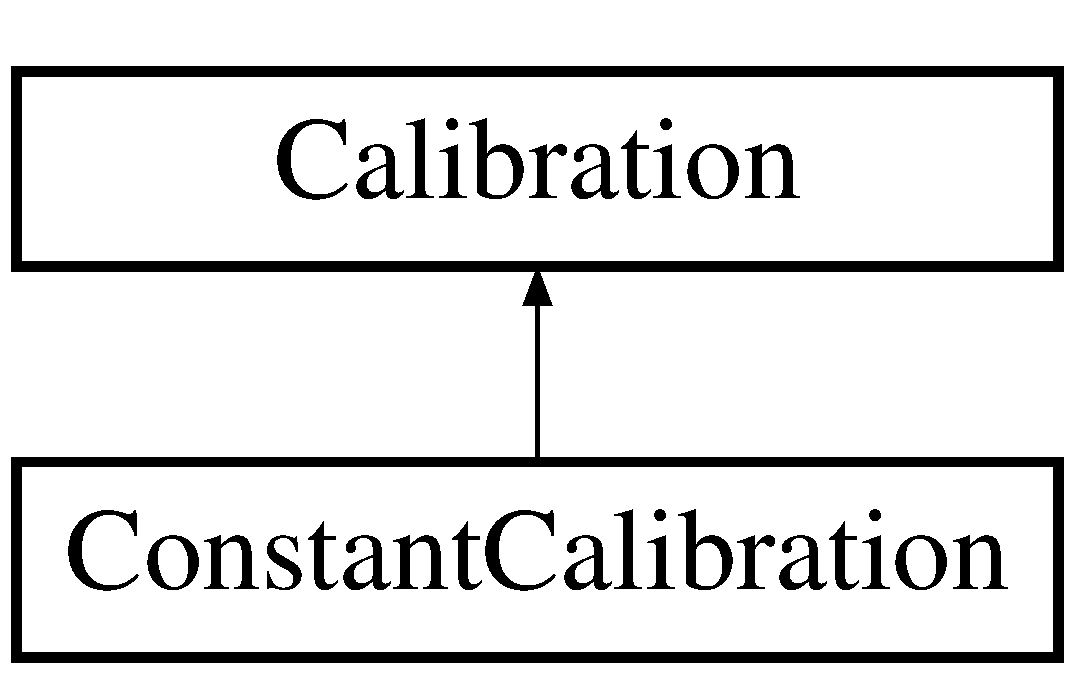
\includegraphics[height=2cm]{classConstantCalibration}
\end{center}
\end{figure}
\subsection*{Public Member Functions}
\begin{DoxyCompactItemize}
\item 
{\bfseries ConstantCalibration} (Float\_\-t a\_\-scale)\label{classConstantCalibration_ae9946996c03d02f0fdbeba232c1038f6}

\item 
Float\_\-t {\bf getCalibratedValue} (UInt\_\-t module\_\-index, UInt\_\-t module\_\-type, UInt\_\-t cell\_\-index, Float\_\-t adc\_\-value) const 
\begin{DoxyCompactList}\small\item\em Determine from a pedestal subtracted ADC value a calibrated value which are identical for this very lazy calibrator. \item\end{DoxyCompactList}\item 
Bool\_\-t {\bf checkForCalibrationConstantsOfModule} (UInt\_\-t module\_\-id, UInt\_\-t module\_\-type, UInt\_\-t n\_\-cells) const 
\begin{DoxyCompactList}\small\item\em Verify that calibration constants exist for a certain module. \item\end{DoxyCompactList}\item 
Int\_\-t {\bf getMiniumADCForMipThreshold} (Float\_\-t mip\_\-energy\_\-fraction) const 
\begin{DoxyCompactList}\small\item\em Get the minimum adc value mips will have for the given energy fraction on all pads. \item\end{DoxyCompactList}\end{DoxyCompactItemize}
\subsection*{Private Attributes}
\begin{DoxyCompactItemize}
\item 
Float\_\-t {\bfseries \_\-scale}\label{classConstantCalibration_a75406a566ee793bd4661588fe071c981}

\end{DoxyCompactItemize}


\subsection{Detailed Description}
Apply the same calibration constant to all values. Useful to perform a very rough calibration such that all the energy parameters, energy dependent bin limits, etc. need not be changed. The collection name of the calibration constant collection is abused to pass the scale paramer (as a string) to this class when created by the kit. 

Definition at line 14 of file ConstantCalibration.hh.

\subsection{Member Function Documentation}
\index{ConstantCalibration@{ConstantCalibration}!checkForCalibrationConstantsOfModule@{checkForCalibrationConstantsOfModule}}
\index{checkForCalibrationConstantsOfModule@{checkForCalibrationConstantsOfModule}!ConstantCalibration@{ConstantCalibration}}
\subsubsection[{checkForCalibrationConstantsOfModule}]{\setlength{\rightskip}{0pt plus 5cm}Bool\_\-t ConstantCalibration::checkForCalibrationConstantsOfModule (UInt\_\-t {\em module\_\-id}, \/  UInt\_\-t {\em module\_\-type}, \/  UInt\_\-t {\em n\_\-cells}) const\hspace{0.3cm}{\ttfamily  [inline, virtual]}}\label{classConstantCalibration_aec30f5342ec651fa61708d2675e14d05}


Verify that calibration constants exist for a certain module. 
\begin{DoxyParams}{Parameters}
\item[{\em module\_\-id}]id Or serial number of a module which uniquely identifies a detector module of a certain type. \item[{\em module\_\-type}]the type of the detector module \item[{\em n\_\-cells}]the number of cells on this module. Return true if calibration constants exist for the given module and the number of cells matches the number of calibration constants. \end{DoxyParams}


Implements {\bf Calibration} \doxyref{}{p.}{classCalibration_a04c8f21c6e77cd3c91c858ca2c9373c4}.

Definition at line 33 of file ConstantCalibration.hh.\index{ConstantCalibration@{ConstantCalibration}!getCalibratedValue@{getCalibratedValue}}
\index{getCalibratedValue@{getCalibratedValue}!ConstantCalibration@{ConstantCalibration}}
\subsubsection[{getCalibratedValue}]{\setlength{\rightskip}{0pt plus 5cm}Float\_\-t ConstantCalibration::getCalibratedValue (UInt\_\-t {\em module\_\-index}, \/  UInt\_\-t {\em module\_\-type}, \/  UInt\_\-t {\em cell\_\-index}, \/  Float\_\-t {\em adc\_\-value}) const\hspace{0.3cm}{\ttfamily  [inline, virtual]}}\label{classConstantCalibration_a347808435c2c9e499af4c9a83d1c6915}


Determine from a pedestal subtracted ADC value a calibrated value which are identical for this very lazy calibrator. 
\begin{DoxyParams}{Parameters}
\item[{\em module\_\-index}]index of the module a module is considered to be a unit which is always calibrated in one calibration run. \item[{\em module\_\-type}]the type of the detector module \item[{\em cell\_\-index}]\item[{\em adc\_\-value}]the ADC value which should be calibrated. \end{DoxyParams}


Implements {\bf Calibration} \doxyref{}{p.}{classCalibration_aca88d93a445ba3021c05dd61b293568c}.

Definition at line 25 of file ConstantCalibration.hh.\index{ConstantCalibration@{ConstantCalibration}!getMiniumADCForMipThreshold@{getMiniumADCForMipThreshold}}
\index{getMiniumADCForMipThreshold@{getMiniumADCForMipThreshold}!ConstantCalibration@{ConstantCalibration}}
\subsubsection[{getMiniumADCForMipThreshold}]{\setlength{\rightskip}{0pt plus 5cm}Int\_\-t ConstantCalibration::getMiniumADCForMipThreshold (Float\_\-t {\em mip\_\-energy\_\-fraction}) const\hspace{0.3cm}{\ttfamily  [inline, virtual]}}\label{classConstantCalibration_ada035fed7a513d3da391bdea2c1d23f7}


Get the minimum adc value mips will have for the given energy fraction on all pads. 
\begin{DoxyParams}{Parameters}
\item[{\em mip\_\-energy\_\-fraction}]the energy in mips \end{DoxyParams}
\begin{DoxyReturn}{Returns}
minimum adc value which is below the given energy on all pads. This method can be used to get the lowest adc value a mip of the given energy fraction will have on all pads. This value is useful to select candidates before actually performing th calibration. This function is intended to be called at the beginning of each event. 
\end{DoxyReturn}


Implements {\bf Calibration} \doxyref{}{p.}{classCalibration_a4e45f1eca0d4fdf19ad76b8f581aee12}.

Definition at line 43 of file ConstantCalibration.hh.

The documentation for this class was generated from the following file:\begin{DoxyCompactItemize}
\item 
ConstantCalibration.hh\end{DoxyCompactItemize}

\section{ConstantCalibrationKit Class Reference}
\label{classConstantCalibrationKit}\index{ConstantCalibrationKit@{ConstantCalibrationKit}}


Create a calibration object which just returns the uncalibrated values.  
Inheritance diagram for ConstantCalibrationKit::\begin{figure}[H]
\begin{center}
\leavevmode
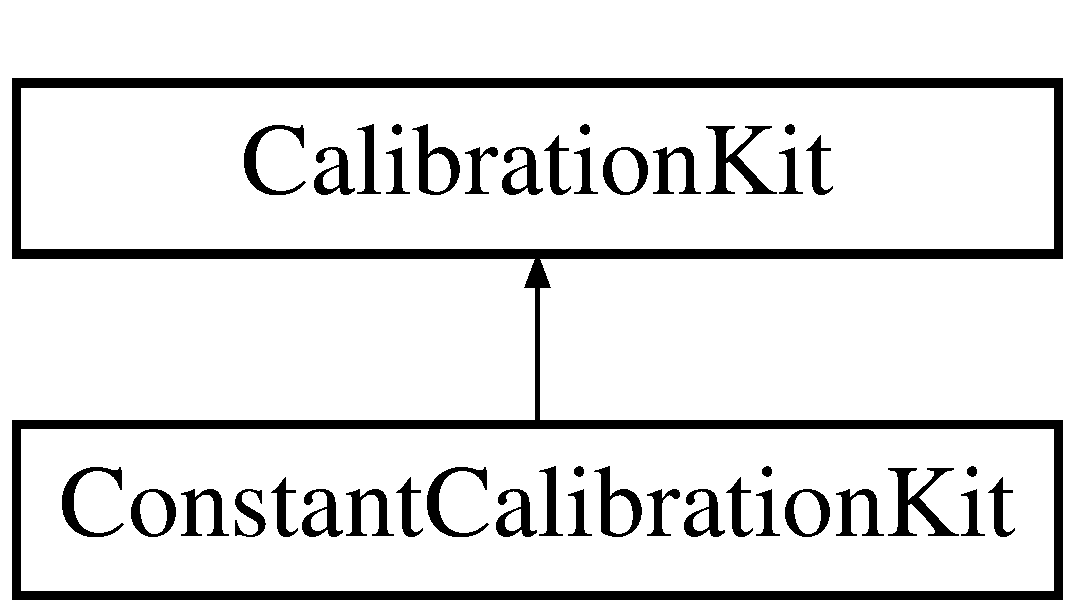
\includegraphics[height=2cm]{classConstantCalibrationKit}
\end{center}
\end{figure}
\subsection*{Public Member Functions}
\begin{DoxyCompactItemize}
\item 
{\bf Calibration} $\ast$ {\bf create} (const std::string \&module\_\-type\_\-col\_\-name, const std::string \&module\_\-calibration\_\-col\_\-name) const 
\begin{DoxyCompactList}\small\item\em Create a constant calibration object. \item\end{DoxyCompactList}\end{DoxyCompactItemize}
\subsection*{Static Protected Attributes}
\begin{DoxyCompactItemize}
\item 
static {\bf ConstantCalibrationKit} {\bfseries \_\-\_\-instance}\label{classConstantCalibrationKit_a7425667eea5619bbf2004d94030b872f}

\end{DoxyCompactItemize}


\subsection{Detailed Description}
Create a calibration object which just returns the uncalibrated values. The collection name of the calibration constant collection is abused to pass the scale paramer to the \doxyref{ConstantCalibration}{p.}{classConstantCalibration} object. \begin{DoxySeeAlso}{See also}
\doxyref{ConstantCalibration}{p.}{classConstantCalibration}. 
\end{DoxySeeAlso}


Definition at line 13 of file ConstantCalibration.cc.

\subsection{Member Function Documentation}
\index{ConstantCalibrationKit@{ConstantCalibrationKit}!create@{create}}
\index{create@{create}!ConstantCalibrationKit@{ConstantCalibrationKit}}
\subsubsection[{create}]{\setlength{\rightskip}{0pt plus 5cm}{\bf Calibration}$\ast$ ConstantCalibrationKit::create (const std::string \& {\em module\_\-type\_\-col\_\-name}, \/  const std::string \& {\em module\_\-calibration\_\-col\_\-name}) const\hspace{0.3cm}{\ttfamily  [inline, virtual]}}\label{classConstantCalibrationKit_a3b84989011be10b816104fdc58963882}


Create a constant calibration object. 
\begin{DoxyParams}{Parameters}
\item[{\em module\_\-type\_\-col\_\-name}]not used. \item[{\em module\_\-calibration\_\-col\_\-name}]converted to a float value and passed as scale to the \doxyref{ConstantCalibration}{p.}{classConstantCalibration} object. \end{DoxyParams}


Implements {\bf CalibrationKit} \doxyref{}{p.}{classCalibrationKit_ab3aea5671d91a7b6f5e839324cf45a70}.

Definition at line 28 of file ConstantCalibration.cc.

The documentation for this class was generated from the following file:\begin{DoxyCompactItemize}
\item 
ConstantCalibration.cc\end{DoxyCompactItemize}

\section{marlin::DhcRawHitProcessor Class Reference}
\label{classmarlin_1_1DhcRawHitProcessor}\index{marlin::DhcRawHitProcessor@{marlin::DhcRawHitProcessor}}


Class to process dhc raw hits and to write out DhcRawCalorimeter Hits.  


{\ttfamily \#include $<$DhcRawHitProcessor.hh$>$}\subsection*{Public Member Functions}
\begin{DoxyCompactItemize}
\item 
virtual Processor $\ast$ {\bfseries newProcessor} ()\label{classmarlin_1_1DhcRawHitProcessor_a60efa733ebac7b3d0a1d3f4b69a57afd}

\item 
void {\bfseries init} ()\label{classmarlin_1_1DhcRawHitProcessor_a17aeafb39578a0ce914906710afcf37c}

\item 
void {\bfseries processEvent} (LCEvent $\ast$evt)\label{classmarlin_1_1DhcRawHitProcessor_a062ebf7771719404738770b8db3967df}

\item 
void {\bfseries end} ()\label{classmarlin_1_1DhcRawHitProcessor_a61469c31a6fb75bfebc73650d91a7d54}

\end{DoxyCompactItemize}


\subsection{Detailed Description}
Class to process dhc raw hits and to write out DhcRawCalorimeter Hits. \begin{DoxyAuthor}{Author}
: R. P�schl DESY 
\end{DoxyAuthor}
\begin{DoxyDate}{Date}
Dec 7 2005 
\end{DoxyDate}


Definition at line 52 of file DhcRawHitProcessor.hh.

The documentation for this class was generated from the following files:\begin{DoxyCompactItemize}
\item 
DhcRawHitProcessor.hh\item 
DhcRawHitProcessor.cc\end{DoxyCompactItemize}

\section{CALICE::ErrorMissingConditionsDataHandler Class Reference}
\label{classCALICE_1_1ErrorMissingConditionsDataHandler}\index{CALICE::ErrorMissingConditionsDataHandler@{CALICE::ErrorMissingConditionsDataHandler}}
\subsection*{Public Member Functions}
\begin{DoxyCompactItemize}
\item 
{\bfseries ErrorMissingConditionsDataHandler} (const std::string \&message)\label{classCALICE_1_1ErrorMissingConditionsDataHandler_a0a85b29547427c53f0c9f5ba5b3070b0}

\item 
{\bfseries ErrorMissingConditionsDataHandler} (const std::string \&message)\label{classCALICE_1_1ErrorMissingConditionsDataHandler_a0a85b29547427c53f0c9f5ba5b3070b0}

\item 
{\bfseries ErrorMissingConditionsDataHandler} (const std::string \&message)\label{classCALICE_1_1ErrorMissingConditionsDataHandler_a0a85b29547427c53f0c9f5ba5b3070b0}

\item 
{\bfseries ErrorMissingConditionsDataHandler} (const std::string \&message)\label{classCALICE_1_1ErrorMissingConditionsDataHandler_a0a85b29547427c53f0c9f5ba5b3070b0}

\end{DoxyCompactItemize}


\subsection{Detailed Description}


Definition at line 19 of file BaseMappingIIProcessor.hh.

The documentation for this class was generated from the following files:\begin{DoxyCompactItemize}
\item 
BaseMappingIIProcessor.hh\item 
fastMappingIIProcessor.hh\item 
ScECALMappingProcessor.hh\item 
VRawADCValueProcessor.hh\end{DoxyCompactItemize}

\section{TBTrackAligner::EventHits Class Reference}
\label{classTBTrackAligner_1_1EventHits}\index{TBTrackAligner::EventHits@{TBTrackAligner::EventHits}}


Method to write the histograms in a ROOT file.  
\subsection*{Data Fields}
\begin{DoxyCompactItemize}
\item 
std::vector$<$ int $>$ {\bfseries \_\-eventHits} [2][4]\label{classTBTrackAligner_1_1EventHits_afb7cf3fe9d066546baa05ea1980bf4a6}

\end{DoxyCompactItemize}


\subsection{Detailed Description}
Method to write the histograms in a ROOT file. 

Definition at line 54 of file TBTrackAligner.hh.

The documentation for this class was generated from the following file:\begin{DoxyCompactItemize}
\item 
TBTrackAligner.hh\end{DoxyCompactItemize}

\section{CALICE::ExtractConfigurationAverageProcessor$<$ KEY, VALUE, OBJECT\_\-TO\_\-AVERAGE $>$ Class Template Reference}
\label{classCALICE_1_1ExtractConfigurationAverageProcessor}\index{CALICE::ExtractConfigurationAverageProcessor@{CALICE::ExtractConfigurationAverageProcessor}}


Processor to determine the channel-\/wise average over any type of configuration over an entire run.  


{\ttfamily \#include $<$ExtractConfigurationAverageProcessor.hh$>$}\subsection*{Public Types}
\begin{DoxyCompactItemize}
\item 
typedef std::map$<$ KEY, AverageValue$<$ VALUE $>$ $>$ {\bfseries AverageValueMap\_\-t}\label{classCALICE_1_1ExtractConfigurationAverageProcessor_a9c98d937494a57cb0002414676ef0a0b}

\item 
typedef AverageValueMap\_\-t::iterator {\bfseries AVM\_\-iterator}\label{classCALICE_1_1ExtractConfigurationAverageProcessor_af2676889c0cabe4ef45a8d0a41953f22}

\item 
typedef AverageValueMap\_\-t::const\_\-iterator {\bfseries AVM\_\-const\_\-iterator}\label{classCALICE_1_1ExtractConfigurationAverageProcessor_ae898392ad5d30a3cf24636368c1f1817}

\item 
typedef KEY(OBJECT\_\-TO\_\-AVERAGE::$\ast$ {\bfseries PMF\_\-KEY} )() const \label{classCALICE_1_1ExtractConfigurationAverageProcessor_ac14ddbcd21b11b49846b2e9f6179806f}

\item 
typedef VALUE(OBJECT\_\-TO\_\-AVERAGE::$\ast$ {\bfseries PMF\_\-VALUE} )() const \label{classCALICE_1_1ExtractConfigurationAverageProcessor_a77c343fefe0aa8c92d90c2c841f2ba0f}

\end{DoxyCompactItemize}
\subsection*{Public Member Functions}
\begin{DoxyCompactItemize}
\item 
{\bfseries ExtractConfigurationAverageProcessor} (const std::string name, PMF\_\-KEY pmf\_\-key, PMF\_\-VALUE pmf\_\-value)\label{classCALICE_1_1ExtractConfigurationAverageProcessor_a8035f64050859ba76161f1432b37b457}

\item 
{\bf ExtractConfigurationAverageProcessor} $\ast$ {\bf newProcessor} ()\label{classCALICE_1_1ExtractConfigurationAverageProcessor_a077ce7a15806f9843796b912eb8fbce7}

\begin{DoxyCompactList}\small\item\em Implements marlin::Processor::newProcessor(). \item\end{DoxyCompactList}\item 
virtual void {\bf init} ()\label{classCALICE_1_1ExtractConfigurationAverageProcessor_a28b4116dd4ec68e02db2c9f2ee17fc74}

\begin{DoxyCompactList}\small\item\em Implements marlin::Processor::init(). \item\end{DoxyCompactList}\item 
virtual void {\bf processEvent} (LCEvent $\ast$evt)\label{classCALICE_1_1ExtractConfigurationAverageProcessor_a7e74ff5efd13293e12977cd11787dbc7}

\begin{DoxyCompactList}\small\item\em Implements marlin::Processor::processEvent(LCEvent$\ast$). \item\end{DoxyCompactList}\item 
virtual void {\bf processRunHeader} (LCRunHeader $\ast$runHeader)\label{classCALICE_1_1ExtractConfigurationAverageProcessor_a3549b7175d1d32b2103f25ead4f5a5fa}

\begin{DoxyCompactList}\small\item\em Implements marlin::Processor::processRunHeader(LCRunHeader$\ast$). \item\end{DoxyCompactList}\item 
virtual void {\bf end} ()\label{classCALICE_1_1ExtractConfigurationAverageProcessor_a877b167e8302d7330d3b2a595ed0e824}

\begin{DoxyCompactList}\small\item\em Implements marlin::Processor::end(). \item\end{DoxyCompactList}\item 
void {\bf print} (std::ostream \&)\label{classCALICE_1_1ExtractConfigurationAverageProcessor_a6c7e3795c5dce5f4430a3fe53a577ff4}

\begin{DoxyCompactList}\small\item\em Print channel wise mean and RMS to output stream. \item\end{DoxyCompactList}\item 
void {\bf writeSimpleFile} (LCCollection $\ast$)\label{classCALICE_1_1ExtractConfigurationAverageProcessor_a6a64edef52110005a069deafdadabb30}

\begin{DoxyCompactList}\small\item\em Store results in LCIO file to be read in by a SimpleFileHandler. \item\end{DoxyCompactList}\item 
void {\bf writeDBFolder} (LCCollection $\ast$)\label{classCALICE_1_1ExtractConfigurationAverageProcessor_ad81f6e7290071ff7ad46f62a268b05a9}

\begin{DoxyCompactList}\small\item\em Store results in LCCD database. \item\end{DoxyCompactList}\end{DoxyCompactItemize}
\subsection*{Protected Member Functions}
\begin{DoxyCompactItemize}
\item 
LCCollection $\ast$ {\bfseries getCollection} ()\label{classCALICE_1_1ExtractConfigurationAverageProcessor_a723f985ee753e55a96b5a1d484e91769}

\end{DoxyCompactItemize}
\subsection*{Protected Attributes}
\begin{DoxyCompactItemize}
\item 
std::string {\bfseries \_\-inColName}\label{classCALICE_1_1ExtractConfigurationAverageProcessor_a6d532e2cc4838f68332367733b4a0bd8}

\item 
std::string {\bfseries \_\-outColName}\label{classCALICE_1_1ExtractConfigurationAverageProcessor_a2c538c11dc9a34d75e7d2a843702f06b}

\item 
std::string {\bfseries \_\-outFileName}\label{classCALICE_1_1ExtractConfigurationAverageProcessor_ab9111f08e45c3959b0ed36aa49bc96aa}

\item 
std::string {\bfseries \_\-dbInit}\label{classCALICE_1_1ExtractConfigurationAverageProcessor_a63aa312d9fb326bd9b868eed4d5d0e70}

\item 
std::string {\bfseries \_\-dbFolder}\label{classCALICE_1_1ExtractConfigurationAverageProcessor_a634cc4a35f2b694cee63d1eff7e06ada}

\item 
std::string {\bfseries \_\-dbDescription}\label{classCALICE_1_1ExtractConfigurationAverageProcessor_a50d196cf146cde52ea5bb0481ce514a6}

\item 
lccd::LCCDTimeStamp {\bfseries \_\-from}\label{classCALICE_1_1ExtractConfigurationAverageProcessor_ab06f9eaf8c5bdfbecc67576231cf32cd}

\item 
lccd::LCCDTimeStamp {\bfseries \_\-till}\label{classCALICE_1_1ExtractConfigurationAverageProcessor_a6ca967970fd97f5134bb45760a1224f8}

\item 
int {\bfseries \_\-selectConf}\label{classCALICE_1_1ExtractConfigurationAverageProcessor_ac22b0611b66e8732f7b8927a8bbf70c6}

\item 
AverageValueMap\_\-t {\bfseries \_\-averageObjects}\label{classCALICE_1_1ExtractConfigurationAverageProcessor_a0fc2d84cee1e5dcb243653b8c2ac15fc}

\item 
const std::string {\bfseries \_\-defaultString}\label{classCALICE_1_1ExtractConfigurationAverageProcessor_a1f8e7e6467b59f155e0a50acfbf19859}

\end{DoxyCompactItemize}
\subsection*{Private Attributes}
\begin{DoxyCompactItemize}
\item 
PMF\_\-KEY {\bfseries \_\-pmf\_\-key}\label{classCALICE_1_1ExtractConfigurationAverageProcessor_a8b33481b90291e374ba3386bc462f378}

\item 
PMF\_\-VALUE {\bfseries \_\-pmf\_\-value}\label{classCALICE_1_1ExtractConfigurationAverageProcessor_a2b24536049c82fd0cbebaee159683451}

\item 
std::string {\bfseries \_\-name}\label{classCALICE_1_1ExtractConfigurationAverageProcessor_adc1336d4d2336e11746598d496e53f7e}

\end{DoxyCompactItemize}


\subsection{Detailed Description}
\subsubsection*{template$<$class KEY, class VALUE, class OBJECT\_\-TO\_\-AVERAGE$>$ class CALICE::ExtractConfigurationAverageProcessor$<$ KEY, VALUE, OBJECT\_\-TO\_\-AVERAGE $>$}

Processor to determine the channel-\/wise average over any type of configuration over an entire run. This processor selects events of a pre-\/defined type of configuration (e.g. pedestal or LED block) and determined the channel-\/wise average over all these events utilizing the AverageValue class. The results get written to screen or stored to LCIO files/LCCD databases in form of SimpleValue objects. Cells are identified by the CellID of the input hits without any further interpretation of the meaning of this number.

\begin{DoxyAuthor}{Author}
{\tt Niels.Meyer@desy.de} 
\end{DoxyAuthor}
\begin{DoxyDate}{Date}
January 2008 
\end{DoxyDate}


Definition at line 29 of file ExtractConfigurationAverageProcessor.hh.

The documentation for this class was generated from the following files:\begin{DoxyCompactItemize}
\item 
ExtractConfigurationAverageProcessor.hh\item 
ExtractConfigurationAverageProcessor.cc\end{DoxyCompactItemize}

\section{CALICE::FastCalib2DProcessor$<$ T, str, M $>$ Class Template Reference}
\label{classCALICE_1_1FastCalib2DProcessor}\index{CALICE::FastCalib2DProcessor@{CALICE::FastCalib2DProcessor}}


Class which handles the application of a certain type T:LCHcalCalibrationObject to an input collection of CaliceHit and writes an output collection of CaliceHit.  


{\ttfamily \#include $<$Fast2DCalibrationProcessor.hh$>$}\subsection*{Public Types}
\begin{DoxyCompactItemize}
\item 
typedef std::map$<$ int, int $>$ {\bfseries parameterMap}\label{classCALICE_1_1FastCalib2DProcessor_a1a398176ac86386375acd10b92a890df}

\end{DoxyCompactItemize}
\subsection*{Public Member Functions}
\begin{DoxyCompactItemize}
\item 
virtual Processor $\ast$ {\bfseries newProcessor} ()\label{classCALICE_1_1FastCalib2DProcessor_aba8e344351415f1bfdc0a0ab54173c27}

\item 
virtual void {\bfseries init} ()\label{classCALICE_1_1FastCalib2DProcessor_a6e39f004ac66605fac85eaf3c2303066}

\item 
void {\bfseries calibrationChanged} (lcio::LCCollection $\ast$col)\label{classCALICE_1_1FastCalib2DProcessor_af9b944cab5d25801f3de9538ca58a5fb}

\item 
void {\bfseries ahcSroModDataColChanged} (lcio::LCCollection $\ast$col)\label{classCALICE_1_1FastCalib2DProcessor_ab5ffcf2162e4d6c1356e19637e407c2c}

\item 
virtual void {\bfseries processEvent} (LCEvent $\ast$evt)\label{classCALICE_1_1FastCalib2DProcessor_a9c91ffa8449e011e0f99d9e2334050ee}

\end{DoxyCompactItemize}
\subsection*{Protected Attributes}
\begin{DoxyCompactItemize}
\item 
std::string {\bfseries \_\-inputColName}\label{classCALICE_1_1FastCalib2DProcessor_ad2a51e143d704ff9d9d33d155381fa2b}

\item 
std::string {\bfseries \_\-parameterColName}\label{classCALICE_1_1FastCalib2DProcessor_aeeddf47e62b3ffa578893b3e040a46c9}

\item 
std::string {\bfseries \_\-outputColName}\label{classCALICE_1_1FastCalib2DProcessor_a67e450d381f338c512bfb61950adc5d8}

\item 
std::string {\bfseries \_\-calColName}\label{classCALICE_1_1FastCalib2DProcessor_acea129179d4f2e8c00901817a63448ab}

\item 
std::string {\bfseries \_\-ahcSroModDataColName}\label{classCALICE_1_1FastCalib2DProcessor_aa1d4ac2e926484e24dd1dbdaf72ea2d5}

\item 
IntVec {\bfseries \_\-modules}\label{classCALICE_1_1FastCalib2DProcessor_a510d4c71eeac41329b513092d81f37e4}

\item 
bool {\bfseries \_\-overwrite}\label{classCALICE_1_1FastCalib2DProcessor_ad4f708e7935bc324ce4df8a2ab97cae2}

\item 
int {\bfseries \_\-zeroSuppression}\label{classCALICE_1_1FastCalib2DProcessor_a3ced223e8bc88a1530a2edd1a2336b5e}

\item 
{\bf CalibrationSet}$<$ T $>$ $\ast$ {\bfseries \_\-calibSet}\label{classCALICE_1_1FastCalib2DProcessor_a8bc3270235a8c869a5b8d72d74709bce}

\item 
M $\ast$ {\bfseries \_\-tempModel}\label{classCALICE_1_1FastCalib2DProcessor_a12febd0f31953e9426311be25b2a4aaa}

\end{DoxyCompactItemize}
\subsection*{Private Attributes}
\begin{DoxyCompactItemize}
\item 
ConditionsChangeDelegator$<$ {\bf FastCalib2DProcessor}$<$ T, str, M $>$ $>$ {\bfseries \_\-calibrationChange}\label{classCALICE_1_1FastCalib2DProcessor_a54d843931315ba73e99210c44c5fca78}

\item 
ConditionsChangeDelegator$<$ {\bf FastCalib2DProcessor}$<$ T, str, M $>$ $>$ {\bfseries \_\-ahcSroModDataChange}\label{classCALICE_1_1FastCalib2DProcessor_a407c59825c0f396ed42aa93e2fa1f3b9}

\item 
lcio::LCCollection $\ast$ {\bfseries \_\-ahcSroModDataCol}\label{classCALICE_1_1FastCalib2DProcessor_ae08612f9f4ea6ec8638027e52549fbe7}

\end{DoxyCompactItemize}


\subsection{Detailed Description}
\subsubsection*{template$<$class T, const char $\ast$ str, class M$>$ class CALICE::FastCalib2DProcessor$<$ T, str, M $>$}

Class which handles the application of a certain type T:LCHcalCalibrationObject to an input collection of CaliceHit and writes an output collection of CaliceHit. 

Definition at line 44 of file Fast2DCalibrationProcessor.hh.

The documentation for this class was generated from the following file:\begin{DoxyCompactItemize}
\item 
Fast2DCalibrationProcessor.hh\end{DoxyCompactItemize}

\section{CALICE::fastMappingIIProcessor Class Reference}
\label{classCALICE_1_1fastMappingIIProcessor}\index{CALICE::fastMappingIIProcessor@{CALICE::fastMappingIIProcessor}}


A class which converts CaliceHits with all calibrations applied into CalorimeterHits.  


{\ttfamily \#include $<$fastMappingIIProcessor.hh$>$}\subsection*{Public Member Functions}
\begin{DoxyCompactItemize}
\item 
virtual Processor $\ast$ {\bfseries newProcessor} ()\label{classCALICE_1_1fastMappingIIProcessor_a84d864c37b51a69f3a5bb3336d11290b}

\item 
virtual void {\bfseries init} ()\label{classCALICE_1_1fastMappingIIProcessor_ad804302fd35900a04771a1647ee9584c}

\item 
virtual void {\bfseries processRunHeader} (LCRunHeader $\ast$run)\label{classCALICE_1_1fastMappingIIProcessor_a4dcdb93e7877928387c0da90288cd243}

\item 
virtual void {\bfseries processEvent} (LCEvent $\ast$evt)\label{classCALICE_1_1fastMappingIIProcessor_ae133d2ea34fae73e13cbbb23d567eef6}

\item 
virtual void {\bfseries check} (LCEvent $\ast$evt)\label{classCALICE_1_1fastMappingIIProcessor_ade7ed6e2dea19fb8b0dce38bececbab4}

\item 
virtual void {\bfseries end} ()\label{classCALICE_1_1fastMappingIIProcessor_a720b8590ee681bb8f78bca09370129b7}

\end{DoxyCompactItemize}
\subsection*{Protected Member Functions}
\begin{DoxyCompactItemize}
\item 
virtual void {\bfseries updateInverseMap} ()\label{classCALICE_1_1fastMappingIIProcessor_ac8554c8b7fe9ed1e0ca25a08eeb8f527}

\item 
virtual void {\bfseries moduleTypeChanged} (lcio::LCCollection $\ast$col)\label{classCALICE_1_1fastMappingIIProcessor_a28c17f0864be618ad5168c9849f1ea01}

\item 
virtual void {\bfseries moduleLocationChanged} (lcio::LCCollection $\ast$col)\label{classCALICE_1_1fastMappingIIProcessor_aaa57f57f89b2b16635dba790b60c212c}

\item 
virtual void {\bfseries moduleConnectionChanged} (lcio::LCCollection $\ast$col)\label{classCALICE_1_1fastMappingIIProcessor_a06bf0a87fa87dd8ed6bd979b8fbeb86b}

\item 
virtual void {\bfseries detectorTransformationChanged} (lcio::LCCollection $\ast$col)\label{classCALICE_1_1fastMappingIIProcessor_a40c88849c1b343429941a7b64553aa63}

\item 
virtual void {\bfseries referenceTransformationChanged} (lcio::LCCollection $\ast$col)\label{classCALICE_1_1fastMappingIIProcessor_a13db4be9a8c31bb01a20915394007d12}

\item 
virtual void {\bfseries stagePositionChanged} (lcio::LCCollection $\ast$col)\label{classCALICE_1_1fastMappingIIProcessor_af962a3c913e7154e79d52ca661526e38}

\end{DoxyCompactItemize}
\subsection*{Protected Attributes}
\begin{DoxyCompactItemize}
\item 
std::string {\bfseries \_\-inputColName}\label{classCALICE_1_1fastMappingIIProcessor_a406af5c65eb5b7fae75a9106701a41ce}

\item 
std::string {\bfseries \_\-outputColName}\label{classCALICE_1_1fastMappingIIProcessor_a0ed73861a50691a4514c0444354d1731}

\item 
std::string {\bfseries \_\-colNameModuleDescription}\label{classCALICE_1_1fastMappingIIProcessor_a915ba9b5892f04844a61ccc01614db62}

\item 
std::string {\bfseries \_\-colNameModuleLocation}\label{classCALICE_1_1fastMappingIIProcessor_ac65181dd90dbb0696ab38e0a8ff6c164}

\item 
std::string {\bfseries \_\-colNameModuleConnection}\label{classCALICE_1_1fastMappingIIProcessor_acfa571d0e14c1121db44ebc355a561f1}

\item 
std::string {\bfseries \_\-colNameDetectorTransformation}\label{classCALICE_1_1fastMappingIIProcessor_af7bcda3e2cda9ee7e41dcf780243c1fd}

\item 
std::string {\bfseries \_\-colNameReferenceTransformation}\label{classCALICE_1_1fastMappingIIProcessor_a7d554688321a42669be0482eac40daf3}

\item 
std::string {\bfseries \_\-colNameStageCollection}\label{classCALICE_1_1fastMappingIIProcessor_ac85b4eccc768ff4ca78280aaadab1402}

\item 
ConditionsChangeDelegator$<$ {\bf fastMappingIIProcessor} $>$ {\bfseries \_\-moduleTypeChange}\label{classCALICE_1_1fastMappingIIProcessor_a3bec21933dd1ca7dec20c925ec4a502a}

\item 
ConditionsChangeDelegator$<$ {\bf fastMappingIIProcessor} $>$ {\bfseries \_\-moduleLocationChange}\label{classCALICE_1_1fastMappingIIProcessor_ac210ebf21a676091fbc1c481c90705b0}

\item 
ConditionsChangeDelegator$<$ {\bf fastMappingIIProcessor} $>$ {\bfseries \_\-moduleConnectionChange}\label{classCALICE_1_1fastMappingIIProcessor_a1313dddb8ca17fb34b960428e1458635}

\item 
ConditionsChangeDelegator$<$ {\bf fastMappingIIProcessor} $>$ {\bfseries \_\-detectorTransformationChange}\label{classCALICE_1_1fastMappingIIProcessor_ad0ad5353b297ad496673e4cddb12b4b6}

\item 
ConditionsChangeDelegator$<$ {\bf fastMappingIIProcessor} $>$ {\bfseries \_\-referenceTransformationChange}\label{classCALICE_1_1fastMappingIIProcessor_a237eeddbe142d84c163d3449224ec161}

\item 
ConditionsChangeDelegator$<$ {\bf fastMappingIIProcessor} $>$ {\bfseries \_\-stagePositionChange}\label{classCALICE_1_1fastMappingIIProcessor_a5f259d239bffa8e68990f72199009810}

\item 
MappingAndAlignment {\bfseries \_\-mapping}\label{classCALICE_1_1fastMappingIIProcessor_ad9dbad825d7b12c0e384651966588f32}

\item 
int {\bfseries \_\-viewConnectionTree}\label{classCALICE_1_1fastMappingIIProcessor_a5512a3532b85add946d846b64112ff3c}

\item 
std::map$<$ unsigned, unsigned $>$ {\bfseries \_\-inverseModuleMap}\label{classCALICE_1_1fastMappingIIProcessor_a608616991c0a6a9aacc5230b676d059c}

\end{DoxyCompactItemize}


\subsection{Detailed Description}
A class which converts CaliceHits with all calibrations applied into CalorimeterHits. \begin{DoxyAuthor}{Author}
S.Schmidt DESY 
\end{DoxyAuthor}
\begin{DoxyDate}{Date}
July 31 2006 
\end{DoxyDate}


Definition at line 30 of file fastMappingIIProcessor.hh.

The documentation for this class was generated from the following files:\begin{DoxyCompactItemize}
\item 
fastMappingIIProcessor.hh\item 
fastMappingIIProcessor.cc\end{DoxyCompactItemize}

\section{CALICE::fastMappingIProcessor Class Reference}
\label{classCALICE_1_1fastMappingIProcessor}\index{CALICE::fastMappingIProcessor@{CALICE::fastMappingIProcessor}}
Inheritance diagram for CALICE::fastMappingIProcessor::\begin{figure}[H]
\begin{center}
\leavevmode
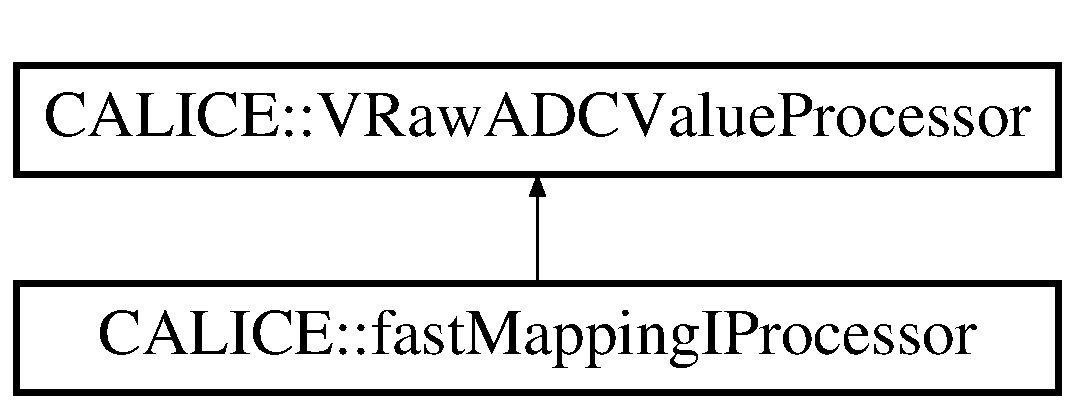
\includegraphics[height=2cm]{classCALICE_1_1fastMappingIProcessor}
\end{center}
\end{figure}
\subsection*{Public Member Functions}
\begin{DoxyCompactItemize}
\item 
virtual Processor $\ast$ {\bfseries newProcessor} ()\label{classCALICE_1_1fastMappingIProcessor_afd4a773dc4a748fd0b0f158145633c1e}

\item 
virtual void {\bfseries init} ()\label{classCALICE_1_1fastMappingIProcessor_a793005abfe7163deb7e8b358f8ba0b1c}

\item 
virtual void {\bfseries processRunHeader} (LCRunHeader $\ast$run)\label{classCALICE_1_1fastMappingIProcessor_a8b6727abbeb2da17115f390a0a98ad27}

\item 
virtual void {\bfseries processEvent} (LCEvent $\ast$evt)\label{classCALICE_1_1fastMappingIProcessor_a1a148ed309dc4126bebefd8b665e99da}

\item 
virtual void {\bfseries check} (LCEvent $\ast$evt)\label{classCALICE_1_1fastMappingIProcessor_a29d4f13330cd1f1a81348412eb9f019f}

\item 
virtual void {\bfseries end} ()\label{classCALICE_1_1fastMappingIProcessor_a68fd91bd4b382f7edf96c209be10afc3}

\end{DoxyCompactItemize}
\subsection*{Protected Attributes}
\begin{DoxyCompactItemize}
\item 
std::string {\bfseries \_\-outputColName}\label{classCALICE_1_1fastMappingIProcessor_a8c3d3a56fa6562d42d5232e1d59793d5}

\item 
int {\bfseries \_\-viewConnectionTree}\label{classCALICE_1_1fastMappingIProcessor_a0c9ffa75645122f519a515e0cc9f03c4}

\item 
int {\bfseries \_\-pickModule}\label{classCALICE_1_1fastMappingIProcessor_a60b71c57578009091da75ae814ac787b}

\end{DoxyCompactItemize}


\subsection{Detailed Description}


Definition at line 26 of file fastMappingIProcessor.hh.

The documentation for this class was generated from the following files:\begin{DoxyCompactItemize}
\item 
fastMappingIProcessor.hh\item 
fastMappingIProcessor.cc\end{DoxyCompactItemize}

\section{CALICE::FilterBadChannels Class Reference}
\label{classCALICE_1_1FilterBadChannels}\index{CALICE::FilterBadChannels@{CALICE::FilterBadChannels}}
\subsection*{Public Member Functions}
\begin{DoxyCompactItemize}
\item 
{\bf FilterBadChannels} $\ast$ {\bfseries newProcessor} ()\label{classCALICE_1_1FilterBadChannels_a06ad29f11701e24e64b82daa9b36b4ba}

\item 
virtual void {\bfseries init} ()\label{classCALICE_1_1FilterBadChannels_ad75699cb8a346a1dcf712a5c4a8709d9}

\item 
virtual void {\bfseries processEvent} (LCEvent $\ast$evt)\label{classCALICE_1_1FilterBadChannels_a96a8e4be917781a9f4612e44ad4f61c3}

\item 
virtual void {\bfseries end} ()\label{classCALICE_1_1FilterBadChannels_ac6a5d35d02c2b6c7dcd81a4c37126b2d}

\end{DoxyCompactItemize}
\subsection*{Private Types}
\begin{DoxyCompactItemize}
\item 
typedef lccd::ConditionsMap$<$ const int, CellQuality $>$ {\bfseries Map\_\-t}\label{classCALICE_1_1FilterBadChannels_ac0393be0651c887dd3b47a40e186ddfa}

\end{DoxyCompactItemize}
\subsection*{Private Attributes}
\begin{DoxyCompactItemize}
\item 
std::string {\bfseries \_\-inColName}\label{classCALICE_1_1FilterBadChannels_a7febc615df3c8f9df80b96a3a23e629d}

\item 
std::string {\bfseries \_\-outColName}\label{classCALICE_1_1FilterBadChannels_af44ac7aeffb09195d2dc225ce3ce903b}

\item 
std::string {\bfseries \_\-statusColName}\label{classCALICE_1_1FilterBadChannels_a011f53f4dda0d7dbc98bf73579d05c95}

\item 
Map\_\-t $\ast$ {\bfseries \_\-statusMap}\label{classCALICE_1_1FilterBadChannels_aa6be96b02055f381369ec71ab5d989fd}

\end{DoxyCompactItemize}


\subsection{Detailed Description}


Definition at line 13 of file FilterBadChannels.hh.

The documentation for this class was generated from the following files:\begin{DoxyCompactItemize}
\item 
FilterBadChannels.hh\item 
FilterBadChannels.cc\end{DoxyCompactItemize}

\section{TBTrack::FitConstants Class Reference}
\label{classTBTrack_1_1FitConstants}\index{TBTrack::FitConstants@{TBTrack::FitConstants}}
\subsection*{Public Types}
\begin{DoxyCompactItemize}
\item 
enum {\bfseries Particle} \{ {\bfseries electron}, 
{\bfseries hadron}
 \}
\item 
enum \{ {\bfseries numberOfInts} = 0
 \}
\item 
enum \{ {\bfseries numberOfFloats} = 0
 \}
\item 
enum \{ {\bfseries numberOfDoubles} = 3 + 2$\ast$2 + 2$\ast$3 + 2$\ast$4 + 2$\ast$2$\ast$21 + 2$\ast$2$\ast$21 + 2$\ast$4 + 4
 \}
\end{DoxyCompactItemize}
\subsection*{Public Member Functions}
\begin{DoxyCompactItemize}
\item 
{\bfseries FitConstants} (unsigned e=1, double err=0.0)\label{classTBTrack_1_1FitConstants_a47ddb6700da0d5c104eb0c369d80911e}

\item 
double {\bfseries pBeam} () const \label{classTBTrack_1_1FitConstants_a133ea6b18d89af235a741119259e0dbb}

\item 
void {\bfseries pBeam} (double p)\label{classTBTrack_1_1FitConstants_a9ce9a2d41aa782c4298a72d5c0eb209c}

\item 
void {\bfseries pBeamScale} (double p)\label{classTBTrack_1_1FitConstants_a6af5bc62244d18b251e7954368ecb9c9}

\item 
double {\bfseries zCalorimeter} () const \label{classTBTrack_1_1FitConstants_acdbec3521ff0b24abf68178cc2f2618b}

\item 
void {\bfseries zCalorimeter} (double z)\label{classTBTrack_1_1FitConstants_af8a150ebd1d2265be0a0640aa58fac87}

\item 
double {\bfseries zBeam} () const \label{classTBTrack_1_1FitConstants_a4375d97e5d050aebd2b9462bbf215c75}

\item 
void {\bfseries zBeam} (double z)\label{classTBTrack_1_1FitConstants_afe66619121004ae499b40341e0d78eaf}

\item 
double {\bfseries beamCoordinate} (unsigned d) const \label{classTBTrack_1_1FitConstants_ad67c0f98da288bdaa426ee94a25056e1}

\item 
void {\bfseries beamCoordinate} (unsigned d, double c)\label{classTBTrack_1_1FitConstants_a999f0fc68f7ddbf17fa49fc77b2ca542}

\item 
double {\bfseries beamAngle} (unsigned d) const \label{classTBTrack_1_1FitConstants_ada6619cbead5a277f3a99df287094fb5}

\item 
void {\bfseries beamAngle} (unsigned d, double a)\label{classTBTrack_1_1FitConstants_a52e266c03c76f8bc27b2eae2f731618d}

\item 
void {\bfseries beamAverage} (unsigned d, double c, double a)\label{classTBTrack_1_1FitConstants_a973118ce9e89a90aaa0453ad2693dc41}

\item 
TMatrixDSym {\bfseries beamSpread} (unsigned d) const \label{classTBTrack_1_1FitConstants_a92a42dc3339b8d8812aaf9b3e96d757d}

\item 
void {\bfseries beamSpread} (unsigned d, const TMatrixDSym \&e)\label{classTBTrack_1_1FitConstants_ad904d24cd02a69767b6935e5a3131aa2}

\item 
double {\bfseries zLayer} (unsigned d, unsigned l) const \label{classTBTrack_1_1FitConstants_a48d3c08ed8a147b4fe34bb0671650fda}

\item 
void {\bfseries zLayer} (unsigned d, unsigned l, double z)\label{classTBTrack_1_1FitConstants_afb9283b46152570709ecf4e2ceba940a}

\item 
TMatrixDSym {\bfseries forwardScattering} (unsigned d, Particle p) const \label{classTBTrack_1_1FitConstants_a5d182698ad7f662247a7f9bf15662cd7}

\item 
void {\bfseries forwardScattering} (unsigned d, Particle p, const TMatrixDSym \&e)\label{classTBTrack_1_1FitConstants_a1ba9942b8faf3f662fd5002a9b2f9d29}

\item 
TMatrixDSym {\bfseries backwardScattering} (unsigned d, Particle p) const \label{classTBTrack_1_1FitConstants_aa2760e9bcaf3ca95fd18d111c2789544}

\item 
void {\bfseries backwardScattering} (unsigned d, Particle p, const TMatrixDSym \&e)\label{classTBTrack_1_1FitConstants_ae3c4ce5580e332d5bcf1c53077f130f7}

\item 
double {\bfseries cError} (unsigned d, unsigned l) const \label{classTBTrack_1_1FitConstants_aa59b427cb93906ae61d18515e656ea05}

\item 
void {\bfseries cError} (unsigned d, unsigned l, double e)\label{classTBTrack_1_1FitConstants_aaa2f3eef3f50ce8ef1c3be75268024c7}

\item 
double {\bfseries probabilityCut} (unsigned nDof) const \label{classTBTrack_1_1FitConstants_a05ec4b2aba5904d2ba510d5b237e740a}

\item 
void {\bfseries probabilityCut} (unsigned nDof, double c)\label{classTBTrack_1_1FitConstants_a19530322178881f38211053231b8719c}

\item 
{\bf TrackFitInitialisation} {\bfseries fitInitialisation} (unsigned xy, unsigned fb, unsigned eh) const \label{classTBTrack_1_1FitConstants_a39d3a5bdfce8fe17387e1470d00543b6}

\item 
void {\bfseries writeIcc} () const \label{classTBTrack_1_1FitConstants_ac5738f5f948c0cee82dab1ca7b5b756b}

\item 
std::ostream \& {\bfseries print} (std::ostream \&o=std::cout, const std::string \&s=\char`\"{}\char`\"{}) const \label{classTBTrack_1_1FitConstants_ad62ddbd9b8fd5f827fccabf35691abf1}

\item 
const int $\ast$ {\bfseries intData} () const \label{classTBTrack_1_1FitConstants_a300c624cc611cb716f86dd7692c6f2ab}

\item 
int $\ast$ {\bfseries intData} ()\label{classTBTrack_1_1FitConstants_a40b7f0a0888a062b84b4c0f47e7aa932}

\item 
const float $\ast$ {\bfseries floatData} () const \label{classTBTrack_1_1FitConstants_ae20c4d5c95c45bad29c9b8f364614e78}

\item 
float $\ast$ {\bfseries floatData} ()\label{classTBTrack_1_1FitConstants_abb376a6b05cc1c2bafb24ba44a230348}

\item 
const double $\ast$ {\bfseries doubleData} () const \label{classTBTrack_1_1FitConstants_a05fa985c01f9de23dbffbe275afa0127}

\item 
double $\ast$ {\bfseries doubleData} ()\label{classTBTrack_1_1FitConstants_a53ba2da4d9d0a108988e207f665c88bd}

\end{DoxyCompactItemize}
\subsection*{Private Member Functions}
\begin{DoxyCompactItemize}
\item 
void {\bfseries convertErrorMatrix} (const double $\ast$d, TMatrixDSym \&e) const \label{classTBTrack_1_1FitConstants_a239bf750e8846e198310ccd5dfc27b51}

\item 
void {\bfseries convertErrorMatrix} (const TMatrixDSym \&e, double $\ast$d)\label{classTBTrack_1_1FitConstants_aed80acea11b9312ca325f0032c2aa624}

\item 
void {\bfseries pBeamScale} (double $\ast$mat, double p)\label{classTBTrack_1_1FitConstants_a9bb5f5ac9c07dfb702e48c48a1dce9ea}

\end{DoxyCompactItemize}
\subsection*{Private Attributes}
\begin{DoxyCompactItemize}
\item 
double {\bfseries \_\-pBeam}\label{classTBTrack_1_1FitConstants_ad065c37d27302f166d583e92ff813e08}

\item 
double {\bfseries \_\-zCalorimeter}\label{classTBTrack_1_1FitConstants_aed3664e51cc6fc58c48e8b2f9ced4b32}

\item 
double {\bfseries \_\-zBeam}\label{classTBTrack_1_1FitConstants_a038e07323028e6f0307fa69685359301}

\item 
double {\bfseries \_\-beamAverage} [2][2]\label{classTBTrack_1_1FitConstants_a701a22a05bbfdc8678fbb11f0a4a6242}

\item 
double {\bfseries \_\-beamSpread} [2][3]\label{classTBTrack_1_1FitConstants_a4d9da5ca3637928a5248e53e6b42cef8}

\item 
double {\bfseries \_\-zLayer} [2][4]\label{classTBTrack_1_1FitConstants_a93f27485f5ce91ac23ffbb9febf4f8f7}

\item 
double {\bfseries \_\-forwardScattering} [2][2][21]\label{classTBTrack_1_1FitConstants_a4a9803ee41a2659da3513e4df42fd349}

\item 
double {\bfseries \_\-backwardScattering} [2][2][21]\label{classTBTrack_1_1FitConstants_ab45f453a56ff58df89b085202ee14bf3}

\item 
double {\bfseries \_\-cError} [2][4]\label{classTBTrack_1_1FitConstants_a2fafd67579669f4e2c291fd30370be36}

\item 
double {\bfseries \_\-probabilityCut} [4]\label{classTBTrack_1_1FitConstants_a7c1fb70c3f9c89d6213b34ccdf88dc67}

\end{DoxyCompactItemize}


\subsection{Detailed Description}


Definition at line 18 of file FitConstants.hh.

The documentation for this class was generated from the following files:\begin{DoxyCompactItemize}
\item 
FitConstants.hh\item 
FitConstants.cc\end{DoxyCompactItemize}

\section{histmgr::FloatHistogram1D Class Reference}
\label{classhistmgr_1_1FloatHistogram1D}\index{histmgr::FloatHistogram1D@{histmgr::FloatHistogram1D}}


A 1-\/dimensional histogram using float values for the bins.  


{\ttfamily \#include $<$FloatHistogram1D.hh$>$}Inheritance diagram for histmgr::FloatHistogram1D::\begin{figure}[H]
\begin{center}
\leavevmode
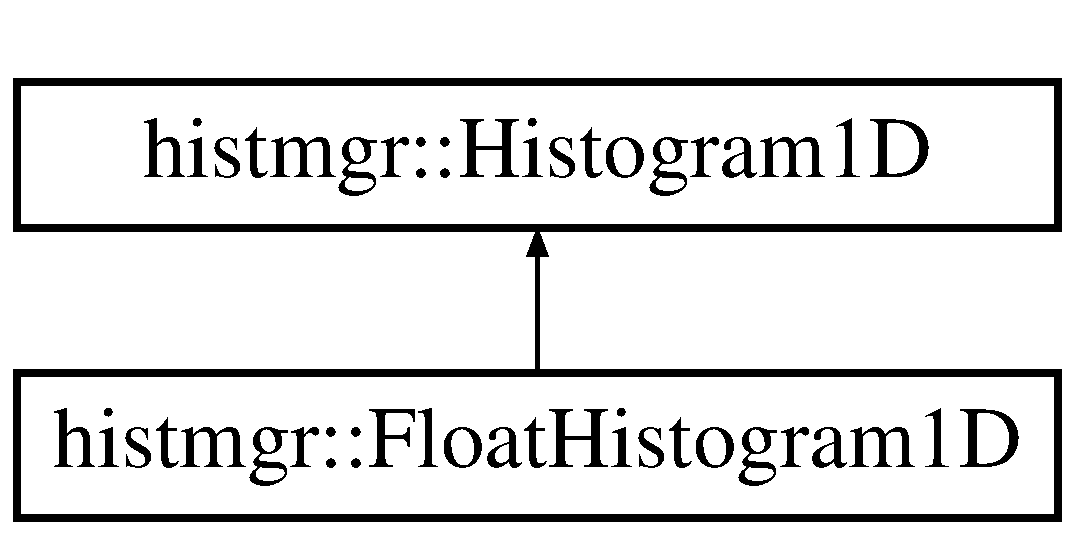
\includegraphics[height=2cm]{classhistmgr_1_1FloatHistogram1D}
\end{center}
\end{figure}
\subsection*{Public Member Functions}
\begin{DoxyCompactItemize}
\item 
{\bf FloatHistogram1D} (UInt\_\-t id, const {\bf HistPar} \&binning)
\begin{DoxyCompactList}\small\item\em Create a histogram with a certain binning. \item\end{DoxyCompactList}\item 
{\bfseries FloatHistogram1D} (lcio::LCObject $\ast$a\_\-obj)\label{classhistmgr_1_1FloatHistogram1D_a1032bc84dcbaa4a6210fb0ee6b5088d7}

\item 
{\bfseries FloatHistogram1D} (const {\bf FloatHistogram1D} \&a)\label{classhistmgr_1_1FloatHistogram1D_af31379e3a83520eac73d5c1609002303}

\item 
void {\bf fill} (Float\_\-t value, Float\_\-t weight=1.)\label{classhistmgr_1_1FloatHistogram1D_aef71989b1c5ad2fc370ee96fb4022213}

\begin{DoxyCompactList}\small\item\em fill a value into the histogram \item\end{DoxyCompactList}\item 
void {\bf reset} ()\label{classhistmgr_1_1FloatHistogram1D_ab6020a2d0902ddc0d6b6f21ae6c579d9}

\begin{DoxyCompactList}\small\item\em reset the histograms and the number of entries \item\end{DoxyCompactList}\item 
void {\bf addToBinContent} (UInt\_\-t bin\_\-index, Float\_\-t value)\label{classhistmgr_1_1FloatHistogram1D_ad0af3ba0d429ed031d43def85d3ca602}

\begin{DoxyCompactList}\small\item\em manipulate a histogram bin \item\end{DoxyCompactList}\item 
void {\bf setBinContent} (UInt\_\-t bin\_\-index, Float\_\-t value)\label{classhistmgr_1_1FloatHistogram1D_a7c3aa74ff2e33c25678d73a0e127ef9f}

\begin{DoxyCompactList}\small\item\em manipulate a histogram bin \item\end{DoxyCompactList}\item 
Float\_\-t {\bfseries binContent} (UInt\_\-t bin\_\-index) const \label{classhistmgr_1_1FloatHistogram1D_a4c772776ba9504a01b41bfdcbc3d4739}

\item 
Float\_\-t {\bfseries overflow} () const \label{classhistmgr_1_1FloatHistogram1D_ac043cc91548219a4ed8b499fa3f213cd}

\item 
Float\_\-t {\bfseries underflow} () const \label{classhistmgr_1_1FloatHistogram1D_a07f92873077aa35c2f8f615595909f8f}

\item 
Float\_\-t {\bfseries mean} () const \label{classhistmgr_1_1FloatHistogram1D_aa62d227b19581c5ad0cb0fa38706c870}

\item 
Float\_\-t {\bf rms} () const 
\begin{DoxyCompactList}\small\item\em Root mean square as defined by ROOT. \item\end{DoxyCompactList}\item 
Float\_\-t {\bf variance} () const 
\begin{DoxyCompactList}\small\item\em Variance. \item\end{DoxyCompactList}\item 
Double\_\-t {\bf integral} (UInt\_\-t first\_\-bin, UInt\_\-t last\_\-bin) const 
\begin{DoxyCompactList}\small\item\em sum contentes of bins within the given range \item\end{DoxyCompactList}\item 
lcio::LCObject $\ast$ {\bfseries clone} () const \label{classhistmgr_1_1FloatHistogram1D_a5edd2500f06f2b1bfd015d9ae4639175}

\end{DoxyCompactItemize}


\subsection{Detailed Description}
A 1-\/dimensional histogram using float values for the bins. 

Definition at line 12 of file FloatHistogram1D.hh.

\subsection{Constructor \& Destructor Documentation}
\index{histmgr::FloatHistogram1D@{histmgr::FloatHistogram1D}!FloatHistogram1D@{FloatHistogram1D}}
\index{FloatHistogram1D@{FloatHistogram1D}!histmgr::FloatHistogram1D@{histmgr::FloatHistogram1D}}
\subsubsection[{FloatHistogram1D}]{\setlength{\rightskip}{0pt plus 5cm}histmgr::FloatHistogram1D::FloatHistogram1D (UInt\_\-t {\em id}, \/  const {\bf HistPar} \& {\em binning})}\label{classhistmgr_1_1FloatHistogram1D_a582ec9a1017297a5e56d159aeb18e2b9}


Create a histogram with a certain binning. 
\begin{DoxyParams}{Parameters}
\item[{\em id}]a unique histogram ID, \item[{\em binning}]number of bins and range of the axis \end{DoxyParams}
\begin{Desc}
\item[{\bf Todo}]a name would be better than an ID but a string can not be easily stored in an LCGenericObject \end{Desc}


Definition at line 8 of file FloatHistogram1D.cc.

References HistPar::nBins(), reset(), and histmgr::Histogram1D::setBinning().

\subsection{Member Function Documentation}
\index{histmgr::FloatHistogram1D@{histmgr::FloatHistogram1D}!integral@{integral}}
\index{integral@{integral}!histmgr::FloatHistogram1D@{histmgr::FloatHistogram1D}}
\subsubsection[{integral}]{\setlength{\rightskip}{0pt plus 5cm}Double\_\-t histmgr::FloatHistogram1D::integral (UInt\_\-t {\em first\_\-bin}, \/  UInt\_\-t {\em last\_\-bin}) const}\label{classhistmgr_1_1FloatHistogram1D_ae4ac2bba1858e9d7750306df22c12903}


sum contentes of bins within the given range 
\begin{DoxyParams}{Parameters}
\item[{\em first\_\-bin}]index of the first bin \item[{\em last\_\-bin}]index of the last bin (included in the sum) \end{DoxyParams}
\begin{DoxyReturn}{Returns}
the sum of the bins 
\end{DoxyReturn}


Definition at line 109 of file FloatHistogram1D.cc.\index{histmgr::FloatHistogram1D@{histmgr::FloatHistogram1D}!rms@{rms}}
\index{rms@{rms}!histmgr::FloatHistogram1D@{histmgr::FloatHistogram1D}}
\subsubsection[{rms}]{\setlength{\rightskip}{0pt plus 5cm}Float\_\-t histmgr::FloatHistogram1D::rms () const}\label{classhistmgr_1_1FloatHistogram1D_a62605cd667af31082c3db712bc6ee337}


Root mean square as defined by ROOT. divided by n 

Definition at line 61 of file FloatHistogram1D.cc.

References histmgr::Histogram1D::entries(), histmgr::Histogram1D::firstBinIndex(), histmgr::Histogram1D::lastBinIndex(), histmgr::Histogram1D::nBins(), histmgr::Histogram1D::xMax(), and histmgr::Histogram1D::xMin().\index{histmgr::FloatHistogram1D@{histmgr::FloatHistogram1D}!variance@{variance}}
\index{variance@{variance}!histmgr::FloatHistogram1D@{histmgr::FloatHistogram1D}}
\subsubsection[{variance}]{\setlength{\rightskip}{0pt plus 5cm}Float\_\-t histmgr::FloatHistogram1D::variance () const}\label{classhistmgr_1_1FloatHistogram1D_acb30c407ee9ad3bbdb85c208d6c8aee6}


Variance. divided by n-\/1 

Definition at line 85 of file FloatHistogram1D.cc.

References histmgr::Histogram1D::entries(), histmgr::Histogram1D::firstBinIndex(), histmgr::Histogram1D::lastBinIndex(), histmgr::Histogram1D::nBins(), histmgr::Histogram1D::xMax(), and histmgr::Histogram1D::xMin().

The documentation for this class was generated from the following files:\begin{DoxyCompactItemize}
\item 
FloatHistogram1D.hh\item 
FloatHistogram1D.cc\end{DoxyCompactItemize}

\section{histmgr::FloatHistogram2D Class Reference}
\label{classhistmgr_1_1FloatHistogram2D}\index{histmgr::FloatHistogram2D@{histmgr::FloatHistogram2D}}


A 1-\/dimensional histogram using float values for the bins.  


{\ttfamily \#include $<$FloatHistogram2D.hh$>$}Inheritance diagram for histmgr::FloatHistogram2D::\begin{figure}[H]
\begin{center}
\leavevmode
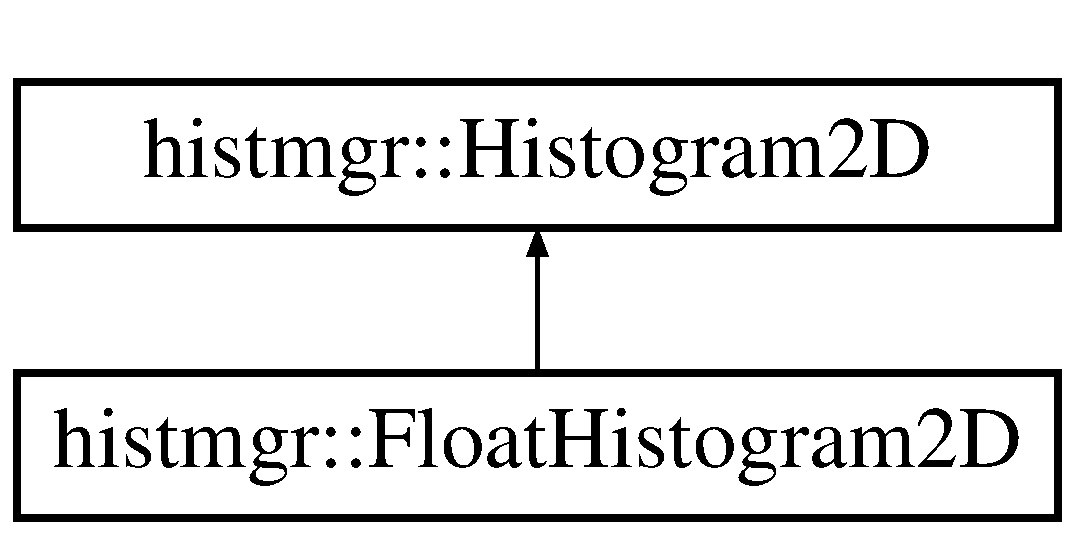
\includegraphics[height=2cm]{classhistmgr_1_1FloatHistogram2D}
\end{center}
\end{figure}
\subsection*{Public Member Functions}
\begin{DoxyCompactItemize}
\item 
{\bf FloatHistogram2D} (UInt\_\-t id, const {\bf HistPar} \&binning\_\-x, const {\bf HistPar} \&binning\_\-y)
\begin{DoxyCompactList}\small\item\em Create a histogram with a certain binning. \item\end{DoxyCompactList}\item 
{\bfseries FloatHistogram2D} (lcio::LCObject $\ast$a\_\-obj)\label{classhistmgr_1_1FloatHistogram2D_ab0dea4b3d379cdb854036719674e71d4}

\item 
{\bfseries FloatHistogram2D} (const {\bf FloatHistogram2D} \&a)\label{classhistmgr_1_1FloatHistogram2D_a68f0f15e037cb32f3d77d6f0984ee3b4}

\item 
void {\bf fill} (Float\_\-t value\_\-x, Float\_\-t value\_\-y, Float\_\-t weight=1.)\label{classhistmgr_1_1FloatHistogram2D_aa817630a68b7456960a13d984032fce6}

\begin{DoxyCompactList}\small\item\em fill a value into the histogram \item\end{DoxyCompactList}\item 
void {\bf reset} ()\label{classhistmgr_1_1FloatHistogram2D_ad3fdcad04762ab70fa346e23d7190b97}

\begin{DoxyCompactList}\small\item\em reset the histograms and the number of entries \item\end{DoxyCompactList}\item 
UInt\_\-t {\bf binIndex} (UInt\_\-t binx\_\-i, UInt\_\-t biny\_\-i) const \label{classhistmgr_1_1FloatHistogram2D_a220db5ab33a4a99a3c1cef4a20b0906c}

\begin{DoxyCompactList}\small\item\em Get the 1d bin index. \item\end{DoxyCompactList}\item 
void {\bf addToBinContent} (UInt\_\-t bin\_\-index, Float\_\-t value)\label{classhistmgr_1_1FloatHistogram2D_a15daa23f7a152fa7b66aa9615aaa5178}

\begin{DoxyCompactList}\small\item\em manipulate a histogram bin \item\end{DoxyCompactList}\item 
void {\bf setBinContent} (UInt\_\-t bin\_\-index, Float\_\-t value)\label{classhistmgr_1_1FloatHistogram2D_ae32ecb4a2dbe9af82e2d9deae0c27ae9}

\begin{DoxyCompactList}\small\item\em manipulate a histogram bin \item\end{DoxyCompactList}\item 
Float\_\-t {\bfseries binContent} (UInt\_\-t bin\_\-index) const \label{classhistmgr_1_1FloatHistogram2D_a49f9dd18dc961e95f62911da156bbc9e}

\item 
Float\_\-t {\bfseries xOverflow} (UInt\_\-t biny\_\-i) const \label{classhistmgr_1_1FloatHistogram2D_a84ee60b090e66f1a1839f73543284ad2}

\item 
Float\_\-t {\bfseries xUnderflow} (UInt\_\-t biny\_\-i) const \label{classhistmgr_1_1FloatHistogram2D_abc8e206e2cac237b73663320202bb573}

\item 
Float\_\-t {\bfseries yOverflow} (UInt\_\-t binx\_\-i) const \label{classhistmgr_1_1FloatHistogram2D_ab3951011e9cf17698a7b3cc5c766446f}

\item 
Float\_\-t {\bfseries yUnderflow} (UInt\_\-t binx\_\-i) const \label{classhistmgr_1_1FloatHistogram2D_aa2267579329064792b162fe320881d42}

\item 
Float\_\-t {\bfseries xUnderflow} () const \label{classhistmgr_1_1FloatHistogram2D_a756024a8658045e2157123e7c4cb3889}

\item 
Float\_\-t {\bfseries xOverflow} () const \label{classhistmgr_1_1FloatHistogram2D_aa0f77dee0d0554a892ef241ade373e07}

\item 
Float\_\-t {\bfseries yUnderflow} () const \label{classhistmgr_1_1FloatHistogram2D_a9615ca79f363ce43a4283a57b2f93bb9}

\item 
Float\_\-t {\bfseries yOverflow} () const \label{classhistmgr_1_1FloatHistogram2D_af1610406b9e3914576f3643158237dfa}

\item 
Float\_\-t {\bfseries xMean} () const \label{classhistmgr_1_1FloatHistogram2D_a7942a45e5b0dd5e353a0d58b62b8de5c}

\item 
Float\_\-t {\bf xRms} (bool natural=false) const 
\begin{DoxyCompactList}\small\item\em Root mean square as defined by ROOT. \item\end{DoxyCompactList}\item 
Float\_\-t {\bf xVariance} () const 
\begin{DoxyCompactList}\small\item\em Variance. \item\end{DoxyCompactList}\item 
Float\_\-t {\bfseries yMean} () const \label{classhistmgr_1_1FloatHistogram2D_a10414e7c9ad34612626fd74572f8add9}

\item 
Float\_\-t {\bf yRms} (bool natural=false) const 
\begin{DoxyCompactList}\small\item\em Root mean square as defined by ROOT. \item\end{DoxyCompactList}\item 
Float\_\-t {\bf yVariance} () const 
\begin{DoxyCompactList}\small\item\em Variance. \item\end{DoxyCompactList}\item 
Double\_\-t {\bf integral} (UInt\_\-t x0\_\-i, UInt\_\-t x1\_\-i, UInt\_\-t y0\_\-i, UInt\_\-t y1\_\-i) const 
\begin{DoxyCompactList}\small\item\em sum contents of bins within the given range \item\end{DoxyCompactList}\item 
lcio::LCObject $\ast$ {\bfseries clone} () const \label{classhistmgr_1_1FloatHistogram2D_a3d2ff7763edb2ad062006f7170a32285}

\end{DoxyCompactItemize}
\subsection*{Private Member Functions}
\begin{DoxyCompactItemize}
\item 
UInt\_\-t {\bfseries nXBinsTotal} () const \label{classhistmgr_1_1FloatHistogram2D_af5a817d2d34a4ee5ecde6dc84b4d5996}

\item 
UInt\_\-t {\bfseries nBinsTotal} () const \label{classhistmgr_1_1FloatHistogram2D_a378ba87874ae6a6d6a2eefc558d3bb7e}

\end{DoxyCompactItemize}


\subsection{Detailed Description}
A 1-\/dimensional histogram using float values for the bins. 

Definition at line 12 of file FloatHistogram2D.hh.

\subsection{Constructor \& Destructor Documentation}
\index{histmgr::FloatHistogram2D@{histmgr::FloatHistogram2D}!FloatHistogram2D@{FloatHistogram2D}}
\index{FloatHistogram2D@{FloatHistogram2D}!histmgr::FloatHistogram2D@{histmgr::FloatHistogram2D}}
\subsubsection[{FloatHistogram2D}]{\setlength{\rightskip}{0pt plus 5cm}histmgr::FloatHistogram2D::FloatHistogram2D (UInt\_\-t {\em id}, \/  const {\bf HistPar} \& {\em binning\_\-x}, \/  const {\bf HistPar} \& {\em binning\_\-y})}\label{classhistmgr_1_1FloatHistogram2D_a2c53fd92a0a2ffa78589ff109acd1b4b}


Create a histogram with a certain binning. 
\begin{DoxyParams}{Parameters}
\item[{\em id}]a unique histogram ID, \item[{\em binning\_\-x}]number of bins and range of the axis \item[{\em binning\_\-y}]number of bins and range of the axis \end{DoxyParams}
\begin{Desc}
\item[{\bf Todo}]a name would be better than an ID but a string can not be easily stored in an LCGenericObject \end{Desc}


Definition at line 8 of file FloatHistogram2D.cc.

References HistPar::nBins(), and reset().

\subsection{Member Function Documentation}
\index{histmgr::FloatHistogram2D@{histmgr::FloatHistogram2D}!integral@{integral}}
\index{integral@{integral}!histmgr::FloatHistogram2D@{histmgr::FloatHistogram2D}}
\subsubsection[{integral}]{\setlength{\rightskip}{0pt plus 5cm}Double\_\-t histmgr::FloatHistogram2D::integral (UInt\_\-t {\em x0\_\-i}, \/  UInt\_\-t {\em x1\_\-i}, \/  UInt\_\-t {\em y0\_\-i}, \/  UInt\_\-t {\em y1\_\-i}) const}\label{classhistmgr_1_1FloatHistogram2D_a32dfa904050e2f247175eb6435147323}


sum contents of bins within the given range 
\begin{DoxyParams}{Parameters}
\item[{\em x0\_\-i}]index of the first bin along x \item[{\em x1\_\-i}]index of the last bin (included in the sum) along x \item[{\em y0\_\-i}]index of the first bin along y \item[{\em y1\_\-i}]index of the last bin (included in the sum) along y \end{DoxyParams}
\begin{DoxyReturn}{Returns}
the sum of the bins 
\end{DoxyReturn}


Definition at line 143 of file FloatHistogram2D.cc.\index{histmgr::FloatHistogram2D@{histmgr::FloatHistogram2D}!xRms@{xRms}}
\index{xRms@{xRms}!histmgr::FloatHistogram2D@{histmgr::FloatHistogram2D}}
\subsubsection[{xRms}]{\setlength{\rightskip}{0pt plus 5cm}Float\_\-t histmgr::FloatHistogram2D::xRms (bool {\em natural} = {\ttfamily false}) const}\label{classhistmgr_1_1FloatHistogram2D_a59c99c39c90a49a62de6678728ced198}


Root mean square as defined by ROOT. divided by n 

Definition at line 65 of file FloatHistogram2D.cc.

References binIndex().\index{histmgr::FloatHistogram2D@{histmgr::FloatHistogram2D}!xVariance@{xVariance}}
\index{xVariance@{xVariance}!histmgr::FloatHistogram2D@{histmgr::FloatHistogram2D}}
\subsubsection[{xVariance}]{\setlength{\rightskip}{0pt plus 5cm}Float\_\-t histmgr::FloatHistogram2D::xVariance () const}\label{classhistmgr_1_1FloatHistogram2D_a96200287a4d48feeb7ae60832c760315}


Variance. divided by n-\/1 \index{histmgr::FloatHistogram2D@{histmgr::FloatHistogram2D}!yRms@{yRms}}
\index{yRms@{yRms}!histmgr::FloatHistogram2D@{histmgr::FloatHistogram2D}}
\subsubsection[{yRms}]{\setlength{\rightskip}{0pt plus 5cm}Float\_\-t histmgr::FloatHistogram2D::yRms (bool {\em natural} = {\ttfamily false}) const}\label{classhistmgr_1_1FloatHistogram2D_a44b5d22fb5fe27a9bac978cac174201a}


Root mean square as defined by ROOT. divided by n 

Definition at line 115 of file FloatHistogram2D.cc.

References binIndex().\index{histmgr::FloatHistogram2D@{histmgr::FloatHistogram2D}!yVariance@{yVariance}}
\index{yVariance@{yVariance}!histmgr::FloatHistogram2D@{histmgr::FloatHistogram2D}}
\subsubsection[{yVariance}]{\setlength{\rightskip}{0pt plus 5cm}Float\_\-t histmgr::FloatHistogram2D::yVariance () const}\label{classhistmgr_1_1FloatHistogram2D_a35e14860e0bd3e2b0370419122f43554}


Variance. divided by n-\/1 

The documentation for this class was generated from the following files:\begin{DoxyCompactItemize}
\item 
FloatHistogram2D.hh\item 
FloatHistogram2D.cc\end{DoxyCompactItemize}

\section{histmgr::GraphCollection\_\-t Class Reference}
\label{classhistmgr_1_1GraphCollection__t}\index{histmgr::GraphCollection\_\-t@{histmgr::GraphCollection\_\-t}}


Light wrapper around a LCCollection to facilitate the handling of collections of graphs.  


{\ttfamily \#include $<$GraphCollection\_\-t.hh$>$}Inheritance diagram for histmgr::GraphCollection\_\-t::\begin{figure}[H]
\begin{center}
\leavevmode
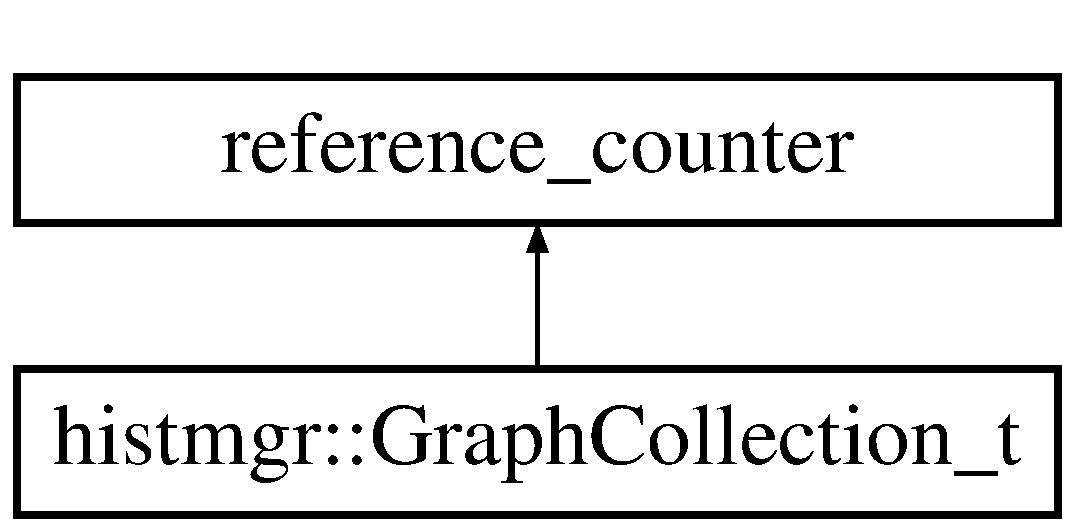
\includegraphics[height=2cm]{classhistmgr_1_1GraphCollection__t}
\end{center}
\end{figure}
\subsection*{Public Member Functions}
\begin{DoxyCompactItemize}
\item 
{\bfseries GraphCollection\_\-t} (const std::string \&collection\_\-name, unsigned int n\_\-graphs, const EVENT::StringVec \&type\_\-names, unsigned int n\_\-expected\_\-values, const EVENT::StringVec \&opt\_\-major\_\-names)  throw (std::bad\_\-alloc, std::runtime\_\-error)\label{classhistmgr_1_1GraphCollection__t_ac8a65ff881a2bcd7831a5eaaab485a7d}

\item 
{\bfseries GraphCollection\_\-t} (const std::string \&collection\_\-name, const std::vector$<$ unsigned int $>$ \&n\_\-graphs, const std::vector$<$ std::string $>$ \&type\_\-names, unsigned int n\_\-expected\_\-values, const std::vector$<$ std::string $>$ \&opt\_\-major\_\-names)  throw (std::bad\_\-alloc, std::runtime\_\-error)\label{classhistmgr_1_1GraphCollection__t_a333affcaa9a51f0c6fb31512a6a7ba24}

\item 
{\bf GraphCollection\_\-t} (lcio::LCCollection $\ast$graphs, lcio::IntVec $\ast$indices)
\item 
{\bf GraphCollection\_\-t} (lcio::LCCollection $\ast$graphs)
\begin{DoxyCompactList}\small\item\em Create a histogram collection from lcio collection. \item\end{DoxyCompactList}\item 
{\bf GraphCollection\_\-t} (const {\bf GraphCollection\_\-t} \&a)\label{classhistmgr_1_1GraphCollection__t_a8beca08f62d11c86c76e861678e0a256}

\begin{DoxyCompactList}\small\item\em copy constructor. \item\end{DoxyCompactList}\item 
void {\bf deleteCollection} ()\label{classhistmgr_1_1GraphCollection__t_a9e80261bb734fb1f63480aee46764ffe}

\begin{DoxyCompactList}\small\item\em delete the histogram collection and the index array This method exists instead of a destrctor to prevent copying the arrays (FIXME) \item\end{DoxyCompactList}\item 
void {\bfseries deleteSharedStorage} ()\label{classhistmgr_1_1GraphCollection__t_aa3c1de2ff8e58f55dd92b68ce42d0535}

\item 
lcio::LCCollection $\ast$ {\bf collection} ()
\begin{DoxyCompactList}\small\item\em get the unique group id \item\end{DoxyCompactList}\item 
const lcio::LCCollection $\ast$ {\bf collection} () const 
\begin{DoxyCompactList}\small\item\em get the collection of graphs (read only). \item\end{DoxyCompactList}\item 
unsigned int {\bf n} () const 
\begin{DoxyCompactList}\small\item\em Get the number of graphs. \item\end{DoxyCompactList}\item 
bool {\bf is2D} () const 
\begin{DoxyCompactList}\small\item\em Check whether the graph collection contains more than one graph group. \item\end{DoxyCompactList}\item 
unsigned int {\bfseries nTypes} () const \label{classhistmgr_1_1GraphCollection__t_aa2092b41bf92f55d260e754ff26e48f2}

\item 
unsigned int {\bf nMajor} () const 
\begin{DoxyCompactList}\small\item\em Get the number of major indices. \item\end{DoxyCompactList}\item 
unsigned int {\bf nMinor} (unsigned int major\_\-index) const 
\begin{DoxyCompactList}\small\item\em Get the number of elements for the collection slice addressed by the given major index. \item\end{DoxyCompactList}\item 
{\bf GraphCollection\_\-t} (const std::string \&collection\_\-name, unsigned int n\_\-graphs, const EVENT::StringVec \&type\_\-names, unsigned int n\_\-expected\_\-values, const EVENT::StringVec \&opt\_\-major\_\-names, bool may\_\-overwrite=false)  throw (std::bad\_\-alloc, std::runtime\_\-error)
\begin{DoxyCompactList}\small\item\em Create a collection of graphs. \item\end{DoxyCompactList}\item 
{\bf GraphCollection\_\-t} (const std::string \&collection\_\-name, const std::vector$<$ int $>$ \&n\_\-graphs, const std::vector$<$ std::string $>$ \&type\_\-names, unsigned int n\_\-expected\_\-values, const std::vector$<$ std::string $>$ \&opt\_\-major\_\-names, bool may\_\-overwrite=false)  throw (std::bad\_\-alloc, std::runtime\_\-error)
\begin{DoxyCompactList}\small\item\em Create a 2D collection of graphs. \item\end{DoxyCompactList}\item 
std::string \& {\bf getMajorName} (unsigned int major\_\-index, unsigned int type\_\-index) const 
\begin{DoxyCompactList}\small\item\em Get the name of the graph group addressed by the major index. \item\end{DoxyCompactList}\item 
std::string \& {\bf getName} (unsigned int major\_\-index, unsigned int minor\_\-index, unsigned int type\_\-index) const 
\begin{DoxyCompactList}\small\item\em Get the full name of the graph which is part of a specfic graph group addressed by the major index. \item\end{DoxyCompactList}\item 
std::string \& {\bf getName} (unsigned int index, unsigned int type\_\-index) const 
\begin{DoxyCompactList}\small\item\em Get the full name of the graph addressed by the index. \item\end{DoxyCompactList}\item 
unsigned int {\bf appendXValue} (double x\_\-value)
\begin{DoxyCompactList}\small\item\em Set the common x value of all the graphs of the graph collection. \item\end{DoxyCompactList}\item 
void {\bf setYValue} (unsigned int major\_\-index, unsigned int minor\_\-index, unsigned int type\_\-index, unsigned int value\_\-index, float a\_\-value)\label{classhistmgr_1_1GraphCollection__t_a2d86a21418a91537e8cb831673b4e88b}

\begin{DoxyCompactList}\small\item\em Set the y-\/value of the adddressed graph. \item\end{DoxyCompactList}\item 
void {\bf setYValue} (unsigned int index, unsigned int type\_\-index, unsigned int value\_\-index, float a\_\-value)\label{classhistmgr_1_1GraphCollection__t_afa630f68afc52b4f115fe35e1c652119}

\begin{DoxyCompactList}\small\item\em Set the y-\/value of the adddressed graph. \item\end{DoxyCompactList}\item 
float {\bf getYValue} (unsigned int index, unsigned int type\_\-index, unsigned int value\_\-index) const \label{classhistmgr_1_1GraphCollection__t_aa897bd01a3c31af0e8b82dbef6b57271}

\begin{DoxyCompactList}\small\item\em Get the y-\/value of the adddressed graph. \item\end{DoxyCompactList}\item 
float {\bf getYValue} (unsigned int major\_\-index, unsigned int minor\_\-index, unsigned int type\_\-index, unsigned int value\_\-index) const \label{classhistmgr_1_1GraphCollection__t_a16f16887fc54666fca9fb47c8d45a6d0}

\begin{DoxyCompactList}\small\item\em Get the y-\/value of the adddressed graph. \item\end{DoxyCompactList}\item 
double {\bf getXValue} (unsigned int index, unsigned int value\_\-index) const \label{classhistmgr_1_1GraphCollection__t_a7dd9e9ac73e5e5ba7bf9f2786a73af0b}

\begin{DoxyCompactList}\small\item\em Get the x-\/value of the adddressed graph. \item\end{DoxyCompactList}\item 
const std::string \& {\bf getName} (unsigned int major\_\-index) const 
\begin{DoxyCompactList}\small\item\em Get the name of the specified element of the graph collection. \item\end{DoxyCompactList}\item 
const std::string \& {\bf getTypeName} (unsigned int type\_\-index) const 
\begin{DoxyCompactList}\small\item\em Get the addressed type name. \item\end{DoxyCompactList}\end{DoxyCompactItemize}
\subsection*{Static Public Attributes}
\begin{DoxyCompactItemize}
\item 
static const std::string {\bfseries \_\-\_\-colorParameterName}\label{classhistmgr_1_1GraphCollection__t_a1934a2578324612aa48e561e45058694}

\item 
static const std::string {\bfseries \_\-\_\-widthParameterName}\label{classhistmgr_1_1GraphCollection__t_ac0f6932a278f313baffc9939f4cb06b3}

\item 
static const std::string {\bfseries \_\-\_\-styleParameterName}\label{classhistmgr_1_1GraphCollection__t_acd025c2ba443992253384db6a7d17a8e}

\item 
static const std::string {\bfseries \_\-\_\-majorColorParameterName}\label{classhistmgr_1_1GraphCollection__t_a8dfd0bff85a2211a1e7090aa43506c4d}

\end{DoxyCompactItemize}
\subsection*{Protected Member Functions}
\begin{DoxyCompactItemize}
\item 
unsigned int {\bf appendFloatValue} (unsigned int full\_\-index, float a\_\-value)\label{classhistmgr_1_1GraphCollection__t_a28fd99da38b507b16d24dff9e7b6b1eb}

\begin{DoxyCompactList}\small\item\em append a new value to the addressed graph, \item\end{DoxyCompactList}\item 
unsigned int {\bf appendValue} (unsigned int full\_\-index, double a\_\-value)\label{classhistmgr_1_1GraphCollection__t_a28ab4fba47b05ef353dd81c76ee4b1b3}

\begin{DoxyCompactList}\small\item\em append a new value to the addressed graph, \item\end{DoxyCompactList}\item 
void {\bf setFloatValue} (unsigned int full\_\-index, unsigned int value\_\-index, float a\_\-value)\label{classhistmgr_1_1GraphCollection__t_a2768ffebabe6eb28b985a622697d263e}

\begin{DoxyCompactList}\small\item\em set a value of the addressed graph, \item\end{DoxyCompactList}\item 
void {\bf setValue} (unsigned int full\_\-index, unsigned int value\_\-index, float a\_\-value)\label{classhistmgr_1_1GraphCollection__t_afe1fbbf9ce02123a6f0d13af1ccf48ab}

\begin{DoxyCompactList}\small\item\em set a value of the addressed graph, \item\end{DoxyCompactList}\item 
double {\bf getValue} (unsigned int full\_\-index, unsigned int value\_\-index) const \label{classhistmgr_1_1GraphCollection__t_a85dd0752c73cfdd78909e1e3e7e55cbf}

\begin{DoxyCompactList}\small\item\em set a value of the addressed graph, \item\end{DoxyCompactList}\item 
double {\bf getFloatValue} (unsigned int full\_\-index, unsigned int value\_\-index) const \label{classhistmgr_1_1GraphCollection__t_a55ab641e3179a97e4d609deea290eb37}

\begin{DoxyCompactList}\small\item\em set a value of the addressed graph, \item\end{DoxyCompactList}\item 
void {\bf addToFloatValue} (unsigned int full\_\-index, unsigned int value\_\-index, float a\_\-value)\label{classhistmgr_1_1GraphCollection__t_a5e747206119488483b0b46c11342dace}

\begin{DoxyCompactList}\small\item\em Add the given value to a certain value of the addressed graph. \item\end{DoxyCompactList}\item 
unsigned int {\bf getIndex} (unsigned int major\_\-index, unsigned int minor\_\-index, unsigned int type\_\-index) const \label{classhistmgr_1_1GraphCollection__t_ae56f52a4ec2a8188b7a3be59c2f90090}

\begin{DoxyCompactList}\small\item\em Calculate the full graph index in case of 2d graph groups. \item\end{DoxyCompactList}\item 
unsigned int {\bf getIndex} (unsigned int index, unsigned int type\_\-index) const \label{classhistmgr_1_1GraphCollection__t_a6babd769d8db88965939660a221ea4b9}

\begin{DoxyCompactList}\small\item\em Calculate the full graph index in case of a flat graph group. \item\end{DoxyCompactList}\item 
EVENT::LCGenericObject $\ast$ {\bfseries getXArray} ()\label{classhistmgr_1_1GraphCollection__t_a2dbf7fc55d252547d24cbac999f0f55e}

\item 
EVENT::LCGenericObject $\ast$ {\bfseries getArray} (unsigned int full\_\-index)\label{classhistmgr_1_1GraphCollection__t_a3e2a4928f2ff0d2249771d76be53c82e}

\end{DoxyCompactItemize}
\subsection*{Static Protected Attributes}
\begin{DoxyCompactItemize}
\item 
static const std::string {\bfseries \_\-\_\-graphNameParameterName}\label{classhistmgr_1_1GraphCollection__t_a1c88428395aa2448fa920b2fd3fc21c1}

\end{DoxyCompactItemize}
\subsection*{Private Member Functions}
\begin{DoxyCompactItemize}
\item 
void {\bf copyNames} () const 
\begin{DoxyCompactList}\small\item\em Assignment operation which deletes the old collections. \item\end{DoxyCompactList}\end{DoxyCompactItemize}
\subsection*{Private Attributes}
\begin{DoxyCompactItemize}
\item 
lcio::LCCollection $\ast$ {\bf \_\-graphCol}\label{classhistmgr_1_1GraphCollection__t_a1196d28c374dfd4e4fdd291542b392f2}

\begin{DoxyCompactList}\small\item\em the histogram collection \item\end{DoxyCompactList}\item 
unsigned int {\bf \_\-nGraphs}\label{classhistmgr_1_1GraphCollection__t_ab839badb20a05434321be1bf9ff36831}

\begin{DoxyCompactList}\small\item\em the number of graphs \item\end{DoxyCompactList}\item 
lcio::IntVec $\ast$ {\bf \_\-majorIndex}
\begin{DoxyCompactList}\small\item\em optional list of offset to form a two dimensional array out of the list. \item\end{DoxyCompactList}\item 
unsigned int {\bf \_\-nTypes}
\begin{DoxyCompactList}\small\item\em number of types. \item\end{DoxyCompactList}\item 
lcio::StringVec {\bf \_\-typeNameList}
\begin{DoxyCompactList}\small\item\em A vector which contains one name for all graphs of the collection or a name for each element (this list is only filled if a names are accessed). \item\end{DoxyCompactList}\item 
lcio::StringVec {\bf \_\-nameList}
\begin{DoxyCompactList}\small\item\em A vector which contains one name for all graphs of the collection or a name for each element. \item\end{DoxyCompactList}\end{DoxyCompactItemize}
\subsection*{Static Private Attributes}
\begin{DoxyCompactItemize}
\item 
static const std::string {\bfseries \_\-\_\-majorIndexParameterName}\label{classhistmgr_1_1GraphCollection__t_adaba3b377fc3c74c4b34fcae6b032849}

\item 
static const std::string {\bfseries \_\-\_\-typeNameParameterName}\label{classhistmgr_1_1GraphCollection__t_aab8c996982d62a8eab7cd537394a07b1}

\item 
static const std::string {\bfseries \_\-\_\-defaultGraphName}\label{classhistmgr_1_1GraphCollection__t_ad7c3d4148ee7dcfbab8485fb3e7872c0}

\end{DoxyCompactItemize}
\subsection*{Friends}
\begin{DoxyCompactItemize}
\item 
class {\bfseries HistMgr}\label{classhistmgr_1_1GraphCollection__t_a3cc85db784d7651390e41024125eb3a0}

\end{DoxyCompactItemize}


\subsection{Detailed Description}
Light wrapper around a LCCollection to facilitate the handling of collections of graphs. All the graphs of the collection share the same x values. The wrapper supports 1 or 2 dimensional collections of graphs. Where each graph collection is composed of several graph groups and each graph group contains a fixed set of graphs of different types. More correctly the collection has a 2 dimensional or 3d diemensional structure. 

Definition at line 27 of file GraphCollection\_\-t.hh.

\subsection{Constructor \& Destructor Documentation}
\index{histmgr::GraphCollection\_\-t@{histmgr::GraphCollection\_\-t}!GraphCollection\_\-t@{GraphCollection\_\-t}}
\index{GraphCollection\_\-t@{GraphCollection\_\-t}!histmgr::GraphCollection_t@{histmgr::GraphCollection\_\-t}}
\subsubsection[{GraphCollection\_\-t}]{\setlength{\rightskip}{0pt plus 5cm}histmgr::GraphCollection\_\-t::GraphCollection\_\-t (lcio::LCCollection $\ast$ {\em graphs}, \/  lcio::IntVec $\ast$ {\em indices})}\label{classhistmgr_1_1GraphCollection__t_a740ae9b62df86330c2734fdf061b119a}

\begin{DoxyParams}{Parameters}
\item[{\em graphs}]the linearised one or two dimensional collection of graphs \item[{\em indices}]optional list of indicies used to give two dimensional access to the histogram list. for each possible index of the first dimension is needed which contains the offset in the list. The second index is added to this offset. \end{DoxyParams}


Definition at line 124 of file GraphCollection\_\-t.cc.

References \_\-graphCol, \_\-majorIndex, \_\-nGraphs, and \_\-nTypes.\index{histmgr::GraphCollection\_\-t@{histmgr::GraphCollection\_\-t}!GraphCollection\_\-t@{GraphCollection\_\-t}}
\index{GraphCollection\_\-t@{GraphCollection\_\-t}!histmgr::GraphCollection_t@{histmgr::GraphCollection\_\-t}}
\subsubsection[{GraphCollection\_\-t}]{\setlength{\rightskip}{0pt plus 5cm}histmgr::GraphCollection\_\-t::GraphCollection\_\-t (lcio::LCCollection $\ast$ {\em graphs})}\label{classhistmgr_1_1GraphCollection__t_a1f8d2f420b8735f4ff9ae71d976f6622}


Create a histogram collection from lcio collection. 
\begin{DoxyParams}{Parameters}
\item[{\em graphs}]the linearised one or two dimensional collection of graphs (two dimensional collections have the collection parameter \char`\"{}major\char`\"{}). The method does not verify whether the lcio collection really is a histogram collection. However, if the collection has the parameter \char`\"{}major\char`\"{} it creates an index vector (costly operation) assuming that it is a 2d array instead of a 1d array(i.e. collection). The unique group id remains undedfined since it is not stored in the lcio collection. \end{DoxyParams}


Definition at line 151 of file GraphCollection\_\-t.cc.

References \_\-graphCol, \_\-majorIndex, \_\-nGraphs, and \_\-nTypes.\index{histmgr::GraphCollection\_\-t@{histmgr::GraphCollection\_\-t}!GraphCollection\_\-t@{GraphCollection\_\-t}}
\index{GraphCollection\_\-t@{GraphCollection\_\-t}!histmgr::GraphCollection_t@{histmgr::GraphCollection\_\-t}}
\subsubsection[{GraphCollection\_\-t}]{\setlength{\rightskip}{0pt plus 5cm}histmgr::GraphCollection\_\-t::GraphCollection\_\-t (const std::string \& {\em collection\_\-name}, \/  unsigned int {\em n\_\-graphs}, \/  const EVENT::StringVec \& {\em type\_\-names}, \/  unsigned int {\em n\_\-expected\_\-values}, \/  const EVENT::StringVec \& {\em opt\_\-major\_\-names}, \/  bool {\em may\_\-overwrite} = {\ttfamily false})  throw (std::bad\_\-alloc, std::runtime\_\-error)}\label{classhistmgr_1_1GraphCollection__t_adb06c0097232711c8f9e3f1cd9f13781}


Create a collection of graphs. Where for each element the given number of graph types is created. 

Definition at line 17 of file GraphCollection\_\-t.cc.\index{histmgr::GraphCollection\_\-t@{histmgr::GraphCollection\_\-t}!GraphCollection\_\-t@{GraphCollection\_\-t}}
\index{GraphCollection\_\-t@{GraphCollection\_\-t}!histmgr::GraphCollection_t@{histmgr::GraphCollection\_\-t}}
\subsubsection[{GraphCollection\_\-t}]{\setlength{\rightskip}{0pt plus 5cm}histmgr::GraphCollection\_\-t::GraphCollection\_\-t (const std::string \& {\em collection\_\-name}, \/  const std::vector$<$ int $>$ \& {\em n\_\-graphs}, \/  const std::vector$<$ std::string $>$ \& {\em type\_\-names}, \/  unsigned int {\em n\_\-expected\_\-values}, \/  const std::vector$<$ std::string $>$ \& {\em opt\_\-major\_\-names}, \/  bool {\em may\_\-overwrite} = {\ttfamily false})  throw (std::bad\_\-alloc, std::runtime\_\-error)}\label{classhistmgr_1_1GraphCollection__t_a6f1026c0d3a09485010e792b05bbc0d2}


Create a 2D collection of graphs. Where for each element of the 2 dimensional collection, the not only a single but for each graph type one.. 

Definition at line 63 of file GraphCollection\_\-t.cc.

\subsection{Member Function Documentation}
\index{histmgr::GraphCollection\_\-t@{histmgr::GraphCollection\_\-t}!appendXValue@{appendXValue}}
\index{appendXValue@{appendXValue}!histmgr::GraphCollection_t@{histmgr::GraphCollection\_\-t}}
\subsubsection[{appendXValue}]{\setlength{\rightskip}{0pt plus 5cm}unsigned int histmgr::GraphCollection\_\-t::appendXValue (double {\em x\_\-value})\hspace{0.3cm}{\ttfamily  [inline]}}\label{classhistmgr_1_1GraphCollection__t_ae9c83cf79211ef808f75343c7c3c3c3d}


Set the common x value of all the graphs of the graph collection. \begin{DoxyReturn}{Returns}
the index of the new value which can be used to set the corresponding values in all the other graphs. 
\end{DoxyReturn}


Definition at line 204 of file GraphCollection\_\-t.hh.

References appendValue().

Referenced by CALICE::AverageHistoryGraphs::processEvent().\index{histmgr::GraphCollection\_\-t@{histmgr::GraphCollection\_\-t}!collection@{collection}}
\index{collection@{collection}!histmgr::GraphCollection_t@{histmgr::GraphCollection\_\-t}}
\subsubsection[{collection}]{\setlength{\rightskip}{0pt plus 5cm}const lcio::LCCollection$\ast$ histmgr::GraphCollection\_\-t::collection () const\hspace{0.3cm}{\ttfamily  [inline]}}\label{classhistmgr_1_1GraphCollection__t_ab8754e9146c1fe855d176fe472413cf1}


get the collection of graphs (read only). The index array needed for the two dimensional acces is added as a parameter named \char`\"{}major\char`\"{}. 

Definition at line 118 of file GraphCollection\_\-t.hh.

References \_\-graphCol.\index{histmgr::GraphCollection\_\-t@{histmgr::GraphCollection\_\-t}!collection@{collection}}
\index{collection@{collection}!histmgr::GraphCollection_t@{histmgr::GraphCollection\_\-t}}
\subsubsection[{collection}]{\setlength{\rightskip}{0pt plus 5cm}lcio::LCCollection$\ast$ histmgr::GraphCollection\_\-t::collection ()\hspace{0.3cm}{\ttfamily  [inline]}}\label{classhistmgr_1_1GraphCollection__t_a10bbe40ded94d3664d9eca002986075e}


get the unique group id get the collection of graphs. The index array needed for the two dimensional acces is added as a parameter named \char`\"{}major\char`\"{}. 

Definition at line 113 of file GraphCollection\_\-t.hh.

References \_\-graphCol.\index{histmgr::GraphCollection\_\-t@{histmgr::GraphCollection\_\-t}!copyNames@{copyNames}}
\index{copyNames@{copyNames}!histmgr::GraphCollection_t@{histmgr::GraphCollection\_\-t}}
\subsubsection[{copyNames}]{\setlength{\rightskip}{0pt plus 5cm}void histmgr::GraphCollection\_\-t::copyNames () const\hspace{0.3cm}{\ttfamily  [inline, private]}}\label{classhistmgr_1_1GraphCollection__t_abf045126bb8f97d49b3e07d776c5724a}


Assignment operation which deletes the old collections. Copy the names from the collection to an accessible vector. The vector of histogram names is attached as a parameter to the LCCollection. 

Definition at line 444 of file GraphCollection\_\-t.hh.

References \_\-graphCol, \_\-nameList, and nMajor().

Referenced by getName().\index{histmgr::GraphCollection\_\-t@{histmgr::GraphCollection\_\-t}!getMajorName@{getMajorName}}
\index{getMajorName@{getMajorName}!histmgr::GraphCollection_t@{histmgr::GraphCollection\_\-t}}
\subsubsection[{getMajorName}]{\setlength{\rightskip}{0pt plus 5cm}std::string\& histmgr::GraphCollection\_\-t::getMajorName (unsigned int {\em major\_\-index}, \/  unsigned int {\em type\_\-index}) const}\label{classhistmgr_1_1GraphCollection__t_a83cbcc31d10a4ee5ad144dbbab667b28}


Get the name of the graph group addressed by the major index. The result is undefined if the graph group is not 2D. \index{histmgr::GraphCollection\_\-t@{histmgr::GraphCollection\_\-t}!getName@{getName}}
\index{getName@{getName}!histmgr::GraphCollection_t@{histmgr::GraphCollection\_\-t}}
\subsubsection[{getName}]{\setlength{\rightskip}{0pt plus 5cm}const std::string\& histmgr::GraphCollection\_\-t::getName (unsigned int {\em major\_\-index}) const\hspace{0.3cm}{\ttfamily  [inline]}}\label{classhistmgr_1_1GraphCollection__t_a89505919c7802e21324986f342afe48e}


Get the name of the specified element of the graph collection. 
\begin{DoxyParams}{Parameters}
\item[{\em major\_\-index}]the index of the histogram element or in case of an 2D histogram array the major index. \end{DoxyParams}
\begin{DoxyReturn}{Returns}
a reference to the name. The index must be valid. 
\end{DoxyReturn}


Definition at line 381 of file GraphCollection\_\-t.hh.

References \_\-nameList, and copyNames().\index{histmgr::GraphCollection\_\-t@{histmgr::GraphCollection\_\-t}!getName@{getName}}
\index{getName@{getName}!histmgr::GraphCollection_t@{histmgr::GraphCollection\_\-t}}
\subsubsection[{getName}]{\setlength{\rightskip}{0pt plus 5cm}std::string\& histmgr::GraphCollection\_\-t::getName (unsigned int {\em index}, \/  unsigned int {\em type\_\-index}) const}\label{classhistmgr_1_1GraphCollection__t_a92a1dd0f7dbd265d4fffc81a7fd77ec6}


Get the full name of the graph addressed by the index. 
\begin{DoxyParams}{Parameters}
\item[{\em index}]the index of the graph in the graph group. \item[{\em type\_\-index}]the index of the graph type. \end{DoxyParams}
\begin{DoxyReturn}{Returns}
the full graph name. The result is undefined if the graph group is not 2D. 
\end{DoxyReturn}
\index{histmgr::GraphCollection\_\-t@{histmgr::GraphCollection\_\-t}!getName@{getName}}
\index{getName@{getName}!histmgr::GraphCollection_t@{histmgr::GraphCollection\_\-t}}
\subsubsection[{getName}]{\setlength{\rightskip}{0pt plus 5cm}std::string\& histmgr::GraphCollection\_\-t::getName (unsigned int {\em major\_\-index}, \/  unsigned int {\em minor\_\-index}, \/  unsigned int {\em type\_\-index}) const}\label{classhistmgr_1_1GraphCollection__t_a2da46bcaf8e6e11f58b7d0dba88061c8}


Get the full name of the graph which is part of a specfic graph group addressed by the major index. 
\begin{DoxyParams}{Parameters}
\item[{\em major\_\-index}]the index of the sub graph group. \item[{\em minor\_\-index}]the index of the graph in the graph group. \item[{\em type\_\-index}]the index of the graph type. \end{DoxyParams}
\begin{DoxyReturn}{Returns}
the full graph name. The result is undefined if the graph group is not 2D. 
\end{DoxyReturn}
\index{histmgr::GraphCollection\_\-t@{histmgr::GraphCollection\_\-t}!getTypeName@{getTypeName}}
\index{getTypeName@{getTypeName}!histmgr::GraphCollection_t@{histmgr::GraphCollection\_\-t}}
\subsubsection[{getTypeName}]{\setlength{\rightskip}{0pt plus 5cm}const std::string\& histmgr::GraphCollection\_\-t::getTypeName (unsigned int {\em type\_\-index}) const\hspace{0.3cm}{\ttfamily  [inline]}}\label{classhistmgr_1_1GraphCollection__t_aec15ce9e41b61e235c0b017d47974a08}


Get the addressed type name. 
\begin{DoxyParams}{Parameters}
\item[{\em type\_\-index}]the index of the type. \end{DoxyParams}
\begin{DoxyReturn}{Returns}
a reference to the type name. The index must be valid. 
\end{DoxyReturn}


Definition at line 397 of file GraphCollection\_\-t.hh.

References \_\-graphCol, and \_\-typeNameList.\index{histmgr::GraphCollection\_\-t@{histmgr::GraphCollection\_\-t}!is2D@{is2D}}
\index{is2D@{is2D}!histmgr::GraphCollection_t@{histmgr::GraphCollection\_\-t}}
\subsubsection[{is2D}]{\setlength{\rightskip}{0pt plus 5cm}bool histmgr::GraphCollection\_\-t::is2D () const\hspace{0.3cm}{\ttfamily  [inline]}}\label{classhistmgr_1_1GraphCollection__t_a67af785a9177d9c41e5f7f3251c2d75b}


Check whether the graph collection contains more than one graph group. \begin{DoxyReturn}{Returns}
true if the graph collection contains more than one graph group which can be addressed by a major index. 
\end{DoxyReturn}


Definition at line 130 of file GraphCollection\_\-t.hh.

References \_\-majorIndex.

Referenced by getIndex().\index{histmgr::GraphCollection\_\-t@{histmgr::GraphCollection\_\-t}!n@{n}}
\index{n@{n}!histmgr::GraphCollection_t@{histmgr::GraphCollection\_\-t}}
\subsubsection[{n}]{\setlength{\rightskip}{0pt plus 5cm}unsigned int histmgr::GraphCollection\_\-t::n () const\hspace{0.3cm}{\ttfamily  [inline]}}\label{classhistmgr_1_1GraphCollection__t_a6ee4913773c2949d5cf3a167038f9a3d}


Get the number of graphs. This value does not take into account that for each graph several types are created. 

Definition at line 123 of file GraphCollection\_\-t.hh.

References \_\-nGraphs.

Referenced by histmgr::HistMgr::fillHistogramCollectionList().\index{histmgr::GraphCollection\_\-t@{histmgr::GraphCollection\_\-t}!nMajor@{nMajor}}
\index{nMajor@{nMajor}!histmgr::GraphCollection_t@{histmgr::GraphCollection\_\-t}}
\subsubsection[{nMajor}]{\setlength{\rightskip}{0pt plus 5cm}unsigned int histmgr::GraphCollection\_\-t::nMajor () const\hspace{0.3cm}{\ttfamily  [inline]}}\label{classhistmgr_1_1GraphCollection__t_ac28f1f78b0326c5e91c40a8d74bb0b49}


Get the number of major indices. The collection is sliced in nMajor slices each having nMinor(major\_\-index) elements. 

Definition at line 144 of file GraphCollection\_\-t.hh.

References \_\-majorIndex.

Referenced by copyNames().\index{histmgr::GraphCollection\_\-t@{histmgr::GraphCollection\_\-t}!nMinor@{nMinor}}
\index{nMinor@{nMinor}!histmgr::GraphCollection_t@{histmgr::GraphCollection\_\-t}}
\subsubsection[{nMinor}]{\setlength{\rightskip}{0pt plus 5cm}unsigned int histmgr::GraphCollection\_\-t::nMinor (unsigned int {\em major\_\-index}) const\hspace{0.3cm}{\ttfamily  [inline]}}\label{classhistmgr_1_1GraphCollection__t_a3428f5d67d892f34f6c5856638873e52}


Get the number of elements for the collection slice addressed by the given major index. The major index must be valid. 

Definition at line 154 of file GraphCollection\_\-t.hh.

References \_\-majorIndex.

\subsection{Field Documentation}
\index{histmgr::GraphCollection\_\-t@{histmgr::GraphCollection\_\-t}!\_\-majorIndex@{\_\-majorIndex}}
\index{\_\-majorIndex@{\_\-majorIndex}!histmgr::GraphCollection_t@{histmgr::GraphCollection\_\-t}}
\subsubsection[{\_\-majorIndex}]{\setlength{\rightskip}{0pt plus 5cm}lcio::IntVec$\ast$ {\bf histmgr::GraphCollection\_\-t::\_\-majorIndex}\hspace{0.3cm}{\ttfamily  [private]}}\label{classhistmgr_1_1GraphCollection__t_aed8f07d8d9e9dc0579ac46468f7102a5}


optional list of offset to form a two dimensional array out of the list. 

Definition at line 459 of file GraphCollection\_\-t.hh.

Referenced by deleteCollection(), getIndex(), GraphCollection\_\-t(), is2D(), nMajor(), and nMinor().\index{histmgr::GraphCollection\_\-t@{histmgr::GraphCollection\_\-t}!\_\-nameList@{\_\-nameList}}
\index{\_\-nameList@{\_\-nameList}!histmgr::GraphCollection_t@{histmgr::GraphCollection\_\-t}}
\subsubsection[{\_\-nameList}]{\setlength{\rightskip}{0pt plus 5cm}lcio::StringVec {\bf histmgr::GraphCollection\_\-t::\_\-nameList}\hspace{0.3cm}{\ttfamily  [mutable, private]}}\label{classhistmgr_1_1GraphCollection__t_a49f968e20a9fa50f9d0d828c61d36028}


A vector which contains one name for all graphs of the collection or a name for each element. 

Definition at line 466 of file GraphCollection\_\-t.hh.

Referenced by copyNames(), and getName().\index{histmgr::GraphCollection\_\-t@{histmgr::GraphCollection\_\-t}!\_\-nTypes@{\_\-nTypes}}
\index{\_\-nTypes@{\_\-nTypes}!histmgr::GraphCollection_t@{histmgr::GraphCollection\_\-t}}
\subsubsection[{\_\-nTypes}]{\setlength{\rightskip}{0pt plus 5cm}unsigned int {\bf histmgr::GraphCollection\_\-t::\_\-nTypes}\hspace{0.3cm}{\ttfamily  [private]}}\label{classhistmgr_1_1GraphCollection__t_ab1a67d796536013057dc680c9f215f36}


number of types. 

Definition at line 461 of file GraphCollection\_\-t.hh.

Referenced by GraphCollection\_\-t().\index{histmgr::GraphCollection\_\-t@{histmgr::GraphCollection\_\-t}!\_\-typeNameList@{\_\-typeNameList}}
\index{\_\-typeNameList@{\_\-typeNameList}!histmgr::GraphCollection_t@{histmgr::GraphCollection\_\-t}}
\subsubsection[{\_\-typeNameList}]{\setlength{\rightskip}{0pt plus 5cm}lcio::StringVec {\bf histmgr::GraphCollection\_\-t::\_\-typeNameList}\hspace{0.3cm}{\ttfamily  [mutable, private]}}\label{classhistmgr_1_1GraphCollection__t_a17189e48d52996372e1fd52c558fbb4a}


A vector which contains one name for all graphs of the collection or a name for each element (this list is only filled if a names are accessed). 

Definition at line 463 of file GraphCollection\_\-t.hh.

Referenced by getTypeName().

The documentation for this class was generated from the following files:\begin{DoxyCompactItemize}
\item 
GraphCollection\_\-t.hh\item 
GraphCollection\_\-t.cc\end{DoxyCompactItemize}

\section{histmgr::HistMgr::Group\_\-t Class Reference}
\label{classhistmgr_1_1HistMgr_1_1Group__t}\index{histmgr::HistMgr::Group\_\-t@{histmgr::HistMgr::Group\_\-t}}
\subsection*{Public Member Functions}
\begin{DoxyCompactItemize}
\item 
void {\bf deleteSharedStorage} ()\label{classhistmgr_1_1HistMgr_1_1Group__t_a7ff0cdee4b9404b88b4afde6a0fbeaac}

\begin{DoxyCompactList}\small\item\em Called by the destructor of \doxyref{KeyMap\_\-t}{p.}{classhistmgr_1_1KeyMap__t} . \item\end{DoxyCompactList}\item 
{\bf HistogramGroupData\_\-t} \& {\bf header} ()
\begin{DoxyCompactList}\small\item\em Get the histogram/graph group header. \item\end{DoxyCompactList}\item 
const {\bf HistogramGroupData\_\-t} \& {\bf header} () const 
\begin{DoxyCompactList}\small\item\em Get the histogram/graph group header. \item\end{DoxyCompactList}\item 
bool {\bf hasHistogramCollections} () const \label{classhistmgr_1_1HistMgr_1_1Group__t_ab56a30ddb87cabb86524d2785caf8529}

\begin{DoxyCompactList}\small\item\em Return true if the Histogram group contains collections of histograms. \item\end{DoxyCompactList}\item 
void {\bf setHistogramCollection} (const {\bf Key\_\-t} \&a\_\-key, {\bf HistogramCollection\_\-t} $\ast$ref)\label{classhistmgr_1_1HistMgr_1_1Group__t_ac4446abfa8ba3589ef1939ce2c407bbe}

\begin{DoxyCompactList}\small\item\em Install the histogram collection and assign the key. \item\end{DoxyCompactList}\item 
bool {\bf histogramCollectionExists} (const {\bf Key\_\-t} \&a\_\-key) const \label{classhistmgr_1_1HistMgr_1_1Group__t_a6dcb61b2793e12470bfd28e4dfeaafef}

\begin{DoxyCompactList}\small\item\em Verify whether a histogram collection exists. \item\end{DoxyCompactList}\item 
{\bf HistogramCollection\_\-t} \& {\bf histogramCollection} (const {\bf Key\_\-t} \&a\_\-key)\label{classhistmgr_1_1HistMgr_1_1Group__t_aba01ed4567e276b2a71494f6755c520f}

\begin{DoxyCompactList}\small\item\em Get the histogram collection addressed by the key. \item\end{DoxyCompactList}\item 
const {\bf HistogramCollection\_\-t} \& {\bf histogramCollection} (const {\bf Key\_\-t} \&a\_\-key) const \label{classhistmgr_1_1HistMgr_1_1Group__t_a98ede72f59c6e9a0f924e9c24fa5a8b4}

\begin{DoxyCompactList}\small\item\em Get the histogram collection addressed by the key (read only). \item\end{DoxyCompactList}\item 
bool {\bf hasHistogram2DCollections} () const \label{classhistmgr_1_1HistMgr_1_1Group__t_a96e6ef55eff3c43cf339716866c82f21}

\begin{DoxyCompactList}\small\item\em Return true if the Histogram group contains collections of 2D histograms. \item\end{DoxyCompactList}\item 
void {\bf setHistogram2DCollection} (const {\bf Key\_\-t} \&a\_\-key, {\bf Histogram2DCollection\_\-t} $\ast$ref)\label{classhistmgr_1_1HistMgr_1_1Group__t_aad3906445d907bfcc905a398503c872a}

\begin{DoxyCompactList}\small\item\em Install the histogram collection and assign the key. \item\end{DoxyCompactList}\item 
bool {\bf histogram2DCollectionExists} (const {\bf Key\_\-t} \&a\_\-key) const \label{classhistmgr_1_1HistMgr_1_1Group__t_a91ecccec34c6ac8359f05262cde6c447}

\begin{DoxyCompactList}\small\item\em Verify whether a histogram collection exists. \item\end{DoxyCompactList}\item 
{\bf Histogram2DCollection\_\-t} \& {\bf histogram2DCollection} (const {\bf Key\_\-t} \&a\_\-key)\label{classhistmgr_1_1HistMgr_1_1Group__t_a39246cff5eaa7174be4bc6144560bc05}

\begin{DoxyCompactList}\small\item\em Get the histogram collection addressed by the key. \item\end{DoxyCompactList}\item 
const {\bf Histogram2DCollection\_\-t} \& {\bf histogram2DCollection} (const {\bf Key\_\-t} \&a\_\-key) const \label{classhistmgr_1_1HistMgr_1_1Group__t_ad9edda850b6752df30366e9cb79c289b}

\begin{DoxyCompactList}\small\item\em Get the histogram collection addressed by the key (read only). \item\end{DoxyCompactList}\item 
bool {\bf hasProfileCollections} () const \label{classhistmgr_1_1HistMgr_1_1Group__t_ab4643d2d3bf49026300bf158ce56f17c}

\begin{DoxyCompactList}\small\item\em Return true if the Histogram group contains collections of profile histograms. \item\end{DoxyCompactList}\item 
void {\bf setProfileCollection} (const {\bf Key\_\-t} \&a\_\-key, {\bf ProfileCollection\_\-t} $\ast$ref)\label{classhistmgr_1_1HistMgr_1_1Group__t_af67b10d61e48586d38e3418f53f82eff}

\begin{DoxyCompactList}\small\item\em Install the histogram collection and assign the key. \item\end{DoxyCompactList}\item 
bool {\bf profileCollectionExists} (const {\bf Key\_\-t} \&a\_\-key) const \label{classhistmgr_1_1HistMgr_1_1Group__t_a730b9b72d809c17387cba4b9724bcf31}

\begin{DoxyCompactList}\small\item\em Verify whether a histogram collection exists. \item\end{DoxyCompactList}\item 
{\bf ProfileCollection\_\-t} \& {\bf profileCollection} (const {\bf Key\_\-t} \&a\_\-key)\label{classhistmgr_1_1HistMgr_1_1Group__t_a4f2b2ee2b2900c5a53fda122d732c559}

\begin{DoxyCompactList}\small\item\em Get the histogram collection addressed by the key. \item\end{DoxyCompactList}\item 
const {\bf ProfileCollection\_\-t} \& {\bf profileCollection} (const {\bf Key\_\-t} \&a\_\-key) const \label{classhistmgr_1_1HistMgr_1_1Group__t_a216742959c54ed5340303264f37849ac}

\begin{DoxyCompactList}\small\item\em Get the histogram collection addressed by the key (read only). \item\end{DoxyCompactList}\item 
bool {\bf hasGraphCollections} () const \label{classhistmgr_1_1HistMgr_1_1Group__t_a0722970a9bc176cb7bdcbaf692c1f68c}

\begin{DoxyCompactList}\small\item\em Return true if the Histogram group contains collections of graphs. \item\end{DoxyCompactList}\item 
void {\bf setGraphCollection} (const {\bf Key\_\-t} \&a\_\-key, {\bf GraphCollection\_\-t} $\ast$ref)\label{classhistmgr_1_1HistMgr_1_1Group__t_a317269f9f9d065c097fd75f77fb6b960}

\begin{DoxyCompactList}\small\item\em Install the histogram collection and assign the key. \item\end{DoxyCompactList}\item 
bool {\bf graphCollectionExists} (const {\bf Key\_\-t} \&a\_\-key) const \label{classhistmgr_1_1HistMgr_1_1Group__t_ae37af4e984bb4080a5437992e623fbe4}

\begin{DoxyCompactList}\small\item\em Verify whether a histogram collection exists. \item\end{DoxyCompactList}\item 
{\bf GraphCollection\_\-t} \& {\bf graphCollection} (const {\bf Key\_\-t} \&a\_\-key)\label{classhistmgr_1_1HistMgr_1_1Group__t_a9cc31d60ad942995646831d197c1ce9b}

\begin{DoxyCompactList}\small\item\em Get the graph collection addressed by the key. \item\end{DoxyCompactList}\item 
const {\bf GraphCollection\_\-t} \& {\bf graphCollection} (const {\bf Key\_\-t} \&a\_\-key) const \label{classhistmgr_1_1HistMgr_1_1Group__t_aedee2016fbc6e3a5215954c16b5b0027}

\begin{DoxyCompactList}\small\item\em Get the graph collection addressed by the key (read only). \item\end{DoxyCompactList}\item 
bool {\bf hasCollection} (ECollectionType type) const \label{classhistmgr_1_1HistMgr_1_1Group__t_a284356fe7c0fd54caba17ccf30a2210c}

\begin{DoxyCompactList}\small\item\em Return true if the collection contains still elements. \item\end{DoxyCompactList}\item 
std::pair$<$ KeyMapBase\_\-t::NameMap\_\-t::const\_\-iterator, KeyMapBase\_\-t::NameMap\_\-t::const\_\-iterator $>$ {\bf nameListIterators} (ECollectionType type) const 
\begin{DoxyCompactList}\small\item\em Get the begin and end iterators of the name list. \item\end{DoxyCompactList}\end{DoxyCompactItemize}
\subsection*{Protected Member Functions}
\begin{DoxyCompactItemize}
\item 
const {\bf KeyMapBase\_\-t} $\ast$ {\bfseries getNameListConst} (ECollectionType \&type) const \label{classhistmgr_1_1HistMgr_1_1Group__t_ada80d7acb301576ad94ab4b992c5ab1e}

\item 
const {\bf KeyMapBase\_\-t} $\ast$ {\bfseries getNameList} (ECollectionType \&type) const \label{classhistmgr_1_1HistMgr_1_1Group__t_a411ea496da41e57b537b8642041b2ee2}

\item 
{\bf KeyMapBase\_\-t} $\ast$ {\bfseries getNameList} (ECollectionType \&type)\label{classhistmgr_1_1HistMgr_1_1Group__t_a48f73dda9c43172b94a94bd7c29af8ea}

\end{DoxyCompactItemize}
\subsection*{Protected Attributes}
\begin{DoxyCompactItemize}
\item 
{\bf HistogramGroupData\_\-t} {\bfseries \_\-header}\label{classhistmgr_1_1HistMgr_1_1Group__t_a29d12ddbcc94cfb35a89b6aaca9f65f5}

\item 
{\bf KeyMap\_\-t}$<$ {\bf accounting\_\-ptr}$<$ {\bf HistogramCollection\_\-t} $>$ $>$ {\bfseries \_\-histogramList}\label{classhistmgr_1_1HistMgr_1_1Group__t_a731e0e40c510e47e4dae48045cbde9ca}

\item 
{\bf KeyMap\_\-t}$<$ {\bf accounting\_\-ptr}$<$ {\bf Histogram2DCollection\_\-t} $>$ $>$ {\bfseries \_\-histogram2DList}\label{classhistmgr_1_1HistMgr_1_1Group__t_a7c230e9216beaaebcc95b71d578aa42e}

\item 
{\bf KeyMap\_\-t}$<$ {\bf accounting\_\-ptr}$<$ {\bf ProfileCollection\_\-t} $>$ $>$ {\bfseries \_\-profileList}\label{classhistmgr_1_1HistMgr_1_1Group__t_a0bef9cfde9749770d1b476497bc4cb7d}

\item 
{\bf KeyMap\_\-t}$<$ {\bf accounting\_\-ptr}$<$ {\bf GraphCollection\_\-t} $>$ $>$ {\bfseries \_\-graphList}\label{classhistmgr_1_1HistMgr_1_1Group__t_a68708db78b489d3d2a907d744dcda55b}

\end{DoxyCompactItemize}
\subsection*{Friends}
\begin{DoxyCompactItemize}
\item 
class {\bfseries HistMgr}\label{classhistmgr_1_1HistMgr_1_1Group__t_a3cc85db784d7651390e41024125eb3a0}

\end{DoxyCompactItemize}


\subsection{Detailed Description}


Definition at line 99 of file HistMgr.hh.

\subsection{Member Function Documentation}
\index{histmgr::HistMgr::Group\_\-t@{histmgr::HistMgr::Group\_\-t}!header@{header}}
\index{header@{header}!histmgr::HistMgr::Group_t@{histmgr::HistMgr::Group\_\-t}}
\subsubsection[{header}]{\setlength{\rightskip}{0pt plus 5cm}const {\bf HistogramGroupData\_\-t}\& histmgr::HistMgr::Group\_\-t::header () const\hspace{0.3cm}{\ttfamily  [inline]}}\label{classhistmgr_1_1HistMgr_1_1Group__t_a175d5209a550475d54e4af0265419b5f}


Get the histogram/graph group header. (read only). The header contains the assignment to files and folders. 

Definition at line 115 of file HistMgr.hh.\index{histmgr::HistMgr::Group\_\-t@{histmgr::HistMgr::Group\_\-t}!header@{header}}
\index{header@{header}!histmgr::HistMgr::Group_t@{histmgr::HistMgr::Group\_\-t}}
\subsubsection[{header}]{\setlength{\rightskip}{0pt plus 5cm}{\bf HistogramGroupData\_\-t}\& histmgr::HistMgr::Group\_\-t::header ()\hspace{0.3cm}{\ttfamily  [inline]}}\label{classhistmgr_1_1HistMgr_1_1Group__t_a278a8749d24f543422bee3f1cacee063}


Get the histogram/graph group header. The header contains the assignment to files and folders. 

Definition at line 110 of file HistMgr.hh.

Referenced by histmgr::HistMgr::assignFileName(), and histmgr::HistMgr::writeHistograms().\index{histmgr::HistMgr::Group\_\-t@{histmgr::HistMgr::Group\_\-t}!nameListIterators@{nameListIterators}}
\index{nameListIterators@{nameListIterators}!histmgr::HistMgr::Group_t@{histmgr::HistMgr::Group\_\-t}}
\subsubsection[{nameListIterators}]{\setlength{\rightskip}{0pt plus 5cm}std::pair$<$KeyMapBase\_\-t::NameMap\_\-t::const\_\-iterator, KeyMapBase\_\-t::NameMap\_\-t::const\_\-iterator$>$ histmgr::HistMgr::Group\_\-t::nameListIterators (ECollectionType {\em type}) const\hspace{0.3cm}{\ttfamily  [inline]}}\label{classhistmgr_1_1HistMgr_1_1Group__t_a6c2929464cba66da95d89c7f9f8aae06}


Get the begin and end iterators of the name list. This can be used to generate a name list of all the elements. 

Definition at line 218 of file HistMgr.hh.

Referenced by histmgr::HistMgr::fillHistogramCollectionList().

The documentation for this class was generated from the following file:\begin{DoxyCompactItemize}
\item 
HistMgr.hh\end{DoxyCompactItemize}

\section{CALICE::HcalTempModel Class Reference}
\label{classCALICE_1_1HcalTempModel}\index{CALICE::HcalTempModel@{CALICE::HcalTempModel}}
Inheritance diagram for CALICE::HcalTempModel::\begin{figure}[H]
\begin{center}
\leavevmode
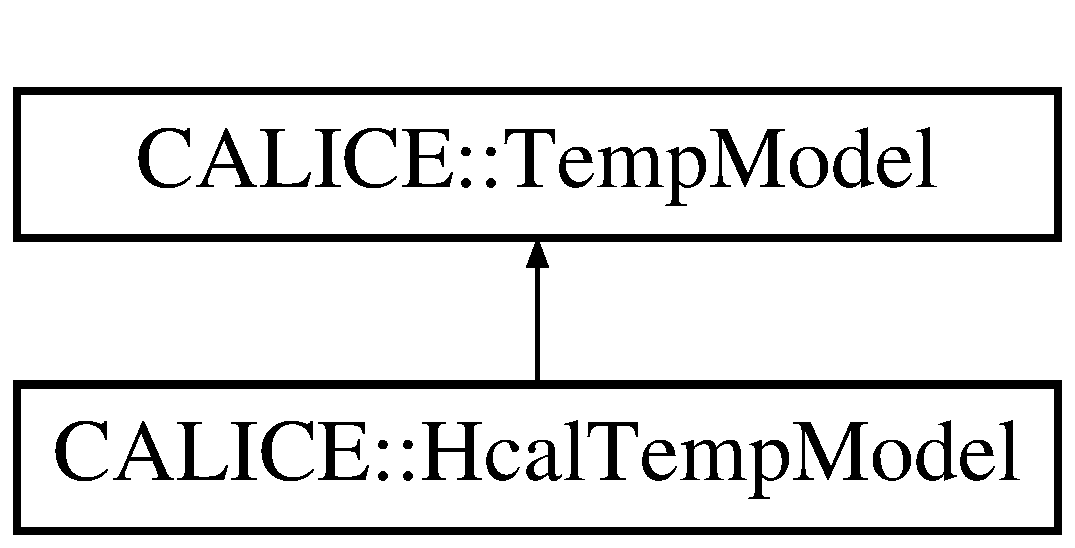
\includegraphics[height=2cm]{classCALICE_1_1HcalTempModel}
\end{center}
\end{figure}
\subsection*{Public Member Functions}
\begin{DoxyCompactItemize}
\item 
virtual float {\bfseries getTemp} (lcio::LCCollection $\ast$col, unsigned moduleID, unsigned CellKey)\label{classCALICE_1_1HcalTempModel_a76afabe82f217f618a8f20098c9cb91b}

\item 
virtual float {\bfseries getTempError} (lcio::LCCollection $\ast$col, unsigned moduleID, unsigned CellKey)\label{classCALICE_1_1HcalTempModel_a4f7355963e4df4c83efb5135a241f785}

\end{DoxyCompactItemize}
\subsection*{Private Attributes}
\begin{DoxyCompactItemize}
\item 
bool {\bfseries \_\-firstWarning}\label{classCALICE_1_1HcalTempModel_a883bb0526e7d1310bedd3f10bfd4e314}

\end{DoxyCompactItemize}


\subsection{Detailed Description}


Definition at line 26 of file HcalTempModel.hh.

The documentation for this class was generated from the following file:\begin{DoxyCompactItemize}
\item 
HcalTempModel.hh\end{DoxyCompactItemize}

\section{histmgr::HistMgr Class Reference}
\label{classhistmgr_1_1HistMgr}\index{histmgr::HistMgr@{histmgr::HistMgr}}


Manages lists of histograms which can be written to prior assigned files.  


{\ttfamily \#include $<$HistMgr.hh$>$}\subsection*{Data Structures}
\begin{DoxyCompactItemize}
\item 
class {\bf Group\_\-t}
\item 
class {\bf HistogramGroupData\_\-t}
\begin{DoxyCompactList}\small\item\em id, destination file and folder of a histogram group \item\end{DoxyCompactList}\end{DoxyCompactItemize}
\subsection*{Public Types}
\begin{DoxyCompactItemize}
\item 
enum {\bfseries ECollectionType} \{ \par
{\bfseries kH1}, 
{\bfseries kH2}, 
{\bfseries kProfile}, 
{\bfseries kGraph}, 
\par
{\bfseries kNTypes}
 \}
\end{DoxyCompactItemize}
\subsection*{Public Member Functions}
\begin{DoxyCompactItemize}
\item 
bool {\bfseries histogramGroupExists} (const {\bf Key\_\-t} \&group\_\-key) const \label{classhistmgr_1_1HistMgr_a4a125aa01302d6ee51520897f5280463}

\item 
{\bf Group\_\-t} \& {\bfseries histogramGroup} (const {\bf Key\_\-t} \&group\_\-key)\label{classhistmgr_1_1HistMgr_ab07a929a02b75ac6f13c08b36533bd9a}

\item 
const {\bf Group\_\-t} \& {\bfseries histogramGroup} (const {\bf Key\_\-t} \&group\_\-key) const \label{classhistmgr_1_1HistMgr_a4bb4d3ffbabd7070f791939a684bab6f}

\item 
{\bf Group\_\-t} \& {\bf getOrCreatehistogramGroup} (const {\bf Key\_\-t} \&group\_\-key)\label{classhistmgr_1_1HistMgr_a3cb22af451aabc860bcee44916d14e04}

\begin{DoxyCompactList}\small\item\em Get the addressed histrogram group. \item\end{DoxyCompactList}\item 
void {\bf createHistogramGroup} (const {\bf Key\_\-t} \&group\_\-key)
\begin{DoxyCompactList}\small\item\em Create an empty histogram group to which histograms can be assigned. \item\end{DoxyCompactList}\item 
lcio::LCCollection $\ast$ {\bf createHistograms} (const {\bf Key\_\-t} \&group\_\-key, const {\bf Key\_\-t} \&collection\_\-key, UInt\_\-t n\_\-hist, const {\bf HistPar} \&par, bool may\_\-overwrite=false)  throw (std::bad\_\-alloc,std::runtime\_\-error)
\begin{DoxyCompactList}\small\item\em create several histograms which will have the same binning and the same name (except of a numeric extension). \item\end{DoxyCompactList}\item 
lcio::LCCollection $\ast$ {\bf createHistograms} (const {\bf Key\_\-t} \&group\_\-key, const {\bf Key\_\-t} \&collection\_\-key, const EVENT::StringVec \&name\_\-list, UInt\_\-t n\_\-hist, const {\bf HistPar} \&par, bool may\_\-overwrite=false)  throw (std::bad\_\-alloc,std::runtime\_\-error)
\begin{DoxyCompactList}\small\item\em create several histograms which will have the same binning and the same name (except of a numeric extension). \item\end{DoxyCompactList}\item 
lcio::LCCollection $\ast$ {\bf createHistograms} (const {\bf Key\_\-t} \&group\_\-key, const {\bf Key\_\-t} \&collection\_\-key, const lcio::IntVec \&n\_\-hist\_\-list, const {\bf HistPar} \&par, bool may\_\-overwrite=false)  throw (std::bad\_\-alloc, std::runtime\_\-error)
\begin{DoxyCompactList}\small\item\em create 2D array of histograms which will all have the same binning and the same name (except of a numeric extension). \item\end{DoxyCompactList}\item 
lcio::LCCollection $\ast$ {\bf createHistograms} (const {\bf Key\_\-t} \&group\_\-key, const {\bf Key\_\-t} \&collection\_\-key, const EVENT::StringVec \&name\_\-list, const lcio::IntVec \&n\_\-hist\_\-list, const {\bf HistPar} \&par, bool may\_\-overwrite=false)  throw (std::bad\_\-alloc, std::runtime\_\-error)
\begin{DoxyCompactList}\small\item\em create 2D array of histograms which will all have the same binning and the same name (except of a numeric extension). \item\end{DoxyCompactList}\item 
lcio::LCCollection $\ast$ {\bf create2DHistograms} (const {\bf Key\_\-t} \&group\_\-key, const {\bf Key\_\-t} \&collection\_\-key, UInt\_\-t n\_\-hist, const {\bf HistPar} \&x\_\-par, const {\bf HistPar} \&y\_\-par, bool may\_\-overwrite=false)  throw (std::bad\_\-alloc,std::runtime\_\-error)
\begin{DoxyCompactList}\small\item\em create several histograms which will have the same binning and the same name (except of a numeric extension). \item\end{DoxyCompactList}\item 
lcio::LCCollection $\ast$ {\bf create2DHistograms} (const {\bf Key\_\-t} \&group\_\-key, const {\bf Key\_\-t} \&collection\_\-key, const EVENT::StringVec \&name\_\-list, UInt\_\-t n\_\-hist, const {\bf HistPar} \&x\_\-par, const {\bf HistPar} \&y\_\-par, bool may\_\-overwrite=false)  throw (std::bad\_\-alloc,std::runtime\_\-error)
\begin{DoxyCompactList}\small\item\em create several histograms which will have the same binning and the same name (except of a numeric extension). \item\end{DoxyCompactList}\item 
lcio::LCCollection $\ast$ {\bf create2DHistograms} (const {\bf Key\_\-t} \&group\_\-key, const {\bf Key\_\-t} \&collection\_\-key, const lcio::IntVec \&n\_\-hist\_\-list, const {\bf HistPar} \&x\_\-par, const {\bf HistPar} \&y\_\-par, bool may\_\-overwrite=false)  throw (std::bad\_\-alloc, std::runtime\_\-error)
\begin{DoxyCompactList}\small\item\em create 2D array of histograms which will all have the same binning and the same name (except of a numeric extension). \item\end{DoxyCompactList}\item 
lcio::LCCollection $\ast$ {\bf create2DHistograms} (const {\bf Key\_\-t} \&group\_\-key, const {\bf Key\_\-t} \&collection\_\-key, const EVENT::StringVec \&name\_\-list, const lcio::IntVec \&n\_\-hist\_\-list, const {\bf HistPar} \&x\_\-par, const {\bf HistPar} \&y\_\-par, bool may\_\-overwrite=false)  throw (std::bad\_\-alloc, std::runtime\_\-error)
\begin{DoxyCompactList}\small\item\em create 2D array of histograms which will all have the same binning and the same name (except of a numeric extension). \item\end{DoxyCompactList}\item 
lcio::LCCollection $\ast$ {\bf createProfile} (const {\bf Key\_\-t} \&group\_\-key, const {\bf Key\_\-t} \&collection\_\-key, UInt\_\-t n\_\-hist, const {\bf HistPar} \&par, bool may\_\-overwrite=false)  throw (std::bad\_\-alloc,std::runtime\_\-error)
\begin{DoxyCompactList}\small\item\em create an array of profile histograms which will all have the same binning of the x-\/axis and the same name (except of a numeric extension). \item\end{DoxyCompactList}\item 
lcio::LCCollection $\ast$ {\bf createProfile} (const {\bf Key\_\-t} \&group\_\-key, const {\bf Key\_\-t} \&collection\_\-key, const EVENT::StringVec \&name\_\-list, UInt\_\-t n\_\-hist, const {\bf HistPar} \&par, bool may\_\-overwrite=false)  throw (std::bad\_\-alloc,std::runtime\_\-error)
\begin{DoxyCompactList}\small\item\em create an array of profile histograms which will all have the same binning of the x-\/axis and the same name (except of a numeric extension). \item\end{DoxyCompactList}\item 
lcio::LCCollection $\ast$ {\bf createProfile} (const {\bf Key\_\-t} \&group\_\-key, const {\bf Key\_\-t} \&collection\_\-key, const lcio::IntVec \&n\_\-hist\_\-list, const {\bf HistPar} \&par, bool may\_\-overwrite=false)  throw (std::bad\_\-alloc, std::runtime\_\-error)
\begin{DoxyCompactList}\small\item\em create 2D array of profile histograms which will all have the same binning and the same name (except of a numeric extension). \item\end{DoxyCompactList}\item 
lcio::LCCollection $\ast$ {\bf createProfile} (const {\bf Key\_\-t} \&group\_\-key, const {\bf Key\_\-t} \&collection\_\-key, const EVENT::StringVec \&name\_\-list, const lcio::IntVec \&n\_\-hist\_\-list, const {\bf HistPar} \&par, bool may\_\-overwrite=false)  throw (std::bad\_\-alloc, std::runtime\_\-error)
\begin{DoxyCompactList}\small\item\em create 2D array of profile histograms which will all have the same binning of the x-\/axis. \item\end{DoxyCompactList}\item 
lcio::LCCollection $\ast$ {\bf createGraphCollection} (const {\bf Key\_\-t} \&group\_\-key, const {\bf Key\_\-t} \&collection\_\-key, unsigned int n\_\-graphs, const EVENT::StringVec \&type\_\-names, unsigned int n\_\-expected\_\-values, const EVENT::StringVec \&opt\_\-major\_\-names, bool may\_\-overwrite=false)  throw (std::bad\_\-alloc, std::runtime\_\-error)
\begin{DoxyCompactList}\small\item\em Create a collection of graphs. \item\end{DoxyCompactList}\item 
lcio::LCCollection $\ast$ {\bfseries createGraphCollection} (const {\bf Key\_\-t} \&group\_\-key, const {\bf Key\_\-t} \&collection\_\-key, const std::vector$<$ int $>$ \&n\_\-graphs, const std::vector$<$ std::string $>$ \&type\_\-names, unsigned int n\_\-expected\_\-values, const std::vector$<$ std::string $>$ \&opt\_\-major\_\-names, bool may\_\-overwrite=false)  throw (std::bad\_\-alloc, std::runtime\_\-error)\label{classhistmgr_1_1HistMgr_a547ce643d66e9a7eb3b2832156da1fdf}

\item 
Double\_\-t {\bf getNEntriesTotal} (const {\bf Key\_\-t} \&group\_\-key) const 
\begin{DoxyCompactList}\small\item\em return the total number of entries in the whole histogram group. \item\end{DoxyCompactList}\item 
{\bf FloatHistogram1D} $\ast$ {\bf getHistogram} (const {\bf Key\_\-t} \&group\_\-key, const {\bf Key\_\-t} \&hist\_\-key, UInt\_\-t index)
\begin{DoxyCompactList}\small\item\em get a histogram of the collection with the given name. \item\end{DoxyCompactList}\item 
const {\bf FloatHistogram1D} $\ast$ {\bf getHistogram} (const {\bf Key\_\-t} \&group\_\-key, const {\bf Key\_\-t} \&hist\_\-key, UInt\_\-t index) const 
\begin{DoxyCompactList}\small\item\em get a histogram of the collection with the given name (read only). \item\end{DoxyCompactList}\item 
const {\bf FloatHistogram1D} $\ast$ {\bf getHistogram} (const {\bf Key\_\-t} \&group\_\-key, const {\bf Key\_\-t} \&hist\_\-key, UInt\_\-t major\_\-index, UInt\_\-t minor\_\-index) const 
\begin{DoxyCompactList}\small\item\em get a histogram of the collection which is organised as a two dimensional array (read only). \item\end{DoxyCompactList}\item 
{\bf FloatHistogram1D} $\ast$ {\bf getHistogram} (const {\bf Key\_\-t} \&group\_\-key, const {\bf Key\_\-t} \&hist\_\-key, UInt\_\-t major\_\-index, UInt\_\-t minor\_\-index)
\begin{DoxyCompactList}\small\item\em get a histogram of the collection which is organised as a two dimensional array. \item\end{DoxyCompactList}\item 
{\bf FloatHistogram2D} $\ast$ {\bf get2DHistogram} (const {\bf Key\_\-t} \&group\_\-key, const {\bf Key\_\-t} \&hist\_\-key, UInt\_\-t index)
\begin{DoxyCompactList}\small\item\em get a 2D histogram of the collection with the given name. \item\end{DoxyCompactList}\item 
const {\bf FloatHistogram2D} $\ast$ {\bf get2DHistogram} (const {\bf Key\_\-t} \&group\_\-key, const {\bf Key\_\-t} \&hist\_\-key, UInt\_\-t index) const 
\begin{DoxyCompactList}\small\item\em get a 2D histogram of the collection with the given name (read only). \item\end{DoxyCompactList}\item 
const {\bf FloatHistogram2D} $\ast$ {\bf get2DHistogram} (const {\bf Key\_\-t} \&group\_\-key, const {\bf Key\_\-t} \&hist\_\-key, UInt\_\-t major\_\-index, UInt\_\-t minor\_\-index) const 
\begin{DoxyCompactList}\small\item\em get a 2D histogram of the collection which is organised as a two dimensional array (read only). \item\end{DoxyCompactList}\item 
{\bf FloatHistogram2D} $\ast$ {\bf get2DHistogram} (const {\bf Key\_\-t} \&group\_\-key, const {\bf Key\_\-t} \&hist\_\-key, UInt\_\-t major\_\-index, UInt\_\-t minor\_\-index)
\begin{DoxyCompactList}\small\item\em get a 2D histogram of the collection which is organised as a two dimensional array. \item\end{DoxyCompactList}\item 
bool {\bf exists} (const {\bf Key\_\-t} \&group\_\-key, const {\bf Key\_\-t} \&hist\_\-key) const \label{classhistmgr_1_1HistMgr_a8367d06ac7fb422b0b65f44d36e435b8}

\begin{DoxyCompactList}\small\item\em verify if a histogram of the given name exists already. \item\end{DoxyCompactList}\item 
{\bf HistogramCollection\_\-t} \& {\bf getHistogramCollection} (const {\bf Key\_\-t} \&group\_\-key, const {\bf Key\_\-t} \&hist\_\-key)\label{classhistmgr_1_1HistMgr_a8589f54841c46f4d807c7d14a944b21b}

\begin{DoxyCompactList}\small\item\em get the one or two dimensional histogram collection. \item\end{DoxyCompactList}\item 
const {\bf HistogramCollection\_\-t} \& {\bf getHistogramCollection} (const {\bf Key\_\-t} \&group\_\-key, const {\bf Key\_\-t} \&hist\_\-key) const \label{classhistmgr_1_1HistMgr_a706bda9b86fbfb7ea67645762c4dd16d}

\begin{DoxyCompactList}\small\item\em get the one or two dimensional histogram collection (read only). \item\end{DoxyCompactList}\item 
{\bf GraphCollection\_\-t} \& {\bf getGraphCollection} (const {\bf Key\_\-t} \&group\_\-key, const {\bf Key\_\-t} \&graph\_\-key)\label{classhistmgr_1_1HistMgr_a6c5ea89b82f7d9df93423976abdf6470}

\begin{DoxyCompactList}\small\item\em Get a graph collection. \item\end{DoxyCompactList}\item 
const {\bf GraphCollection\_\-t} \& {\bf getGraphCollection} (const {\bf Key\_\-t} \&group\_\-key, const {\bf Key\_\-t} \&graph\_\-key) const 
\begin{DoxyCompactList}\small\item\em Get a graph collection. \item\end{DoxyCompactList}\item 
{\bf Histogram2DCollection\_\-t} \& {\bf getHistogram2DCollection} (const {\bf Key\_\-t} \&group\_\-key, const {\bf Key\_\-t} \&histogram2D\_\-key)\label{classhistmgr_1_1HistMgr_a3daca1d8debe8c217365403d0fd6e6a4}

\begin{DoxyCompactList}\small\item\em Get a histogram2D collection. \item\end{DoxyCompactList}\item 
const {\bf Histogram2DCollection\_\-t} \& {\bf getHistogram2DCollection} (const {\bf Key\_\-t} \&group\_\-key, const {\bf Key\_\-t} \&histogram2D\_\-key) const 
\begin{DoxyCompactList}\small\item\em Get a histogram2D collection. \item\end{DoxyCompactList}\item 
{\bf ProfileCollection\_\-t} \& {\bf getProfileCollection} (const {\bf Key\_\-t} \&group\_\-key, const {\bf Key\_\-t} \&profile\_\-key)\label{classhistmgr_1_1HistMgr_a9580175c8b4af1862261acddd6f7b872}

\begin{DoxyCompactList}\small\item\em Get a profile collection. \item\end{DoxyCompactList}\item 
const {\bf ProfileCollection\_\-t} \& {\bf getProfileCollection} (const {\bf Key\_\-t} \&group\_\-key, const {\bf Key\_\-t} \&profile\_\-key) const 
\begin{DoxyCompactList}\small\item\em Get a profile collection. \item\end{DoxyCompactList}\item 
void {\bf assignFileName} (const {\bf Key\_\-t} \&group\_\-key, const std::string \&file\_\-name, const std::string \&folder\_\-name=\char`\"{}\char`\"{})
\begin{DoxyCompactList}\small\item\em get the histogram collection of the given name (read only) The collection must not be deleted. \item\end{DoxyCompactList}\item 
void {\bf warnOnUnassigned} ()
\begin{DoxyCompactList}\small\item\em Issue a warning for all histogram groups which are not assigned to a file. \item\end{DoxyCompactList}\item 
void {\bf writeHistograms} (bool snapshot=false)
\begin{DoxyCompactList}\small\item\em write all histograms groups to the assigned files. \item\end{DoxyCompactList}\item 
void {\bf writeHistograms} (const {\bf Key\_\-t} \&group\_\-key, bool snapshot=false)
\begin{DoxyCompactList}\small\item\em write all histograms of the specified group to the assigned root file. \item\end{DoxyCompactList}\item 
void {\bf registerWriter} (const std::string \&name, {\bf HistWriterKit} $\ast$kit)
\begin{DoxyCompactList}\small\item\em register a histogram writer. \item\end{DoxyCompactList}\item 
void {\bfseries listRegisteredGroups} () const \label{classhistmgr_1_1HistMgr_a9454383d4576085b061e68e912dc1d09}

\item 
UInt\_\-t {\bf getNGroups} () const \label{classhistmgr_1_1HistMgr_a5e6a8a27e9e66d2e0d9e1fd4db24d922}

\begin{DoxyCompactList}\small\item\em Get the number of groups. \item\end{DoxyCompactList}\item 
void {\bf lockGroup} (const {\bf Key\_\-t} \&group\_\-key)
\begin{DoxyCompactList}\small\item\em Lock a histogram group. \item\end{DoxyCompactList}\item 
void {\bf unlockGroup} (const {\bf Key\_\-t} \&group\_\-key)
\begin{DoxyCompactList}\small\item\em Release the lock on the histogram group. \item\end{DoxyCompactList}\item 
bool {\bf hasLockedGroups} () const \label{classhistmgr_1_1HistMgr_a961080e7358f08fd2f5382038e6952ba}

\begin{DoxyCompactList}\small\item\em Return true if some of the groups are locked. \item\end{DoxyCompactList}\item 
void {\bf fillGroupList} (std::vector$<$ std::string $>$ \&dest\_\-group\_\-list) const 
\begin{DoxyCompactList}\small\item\em Copy the groups names into the given vecotor. \item\end{DoxyCompactList}\item 
void {\bf fillHistogramCollectionList} (const {\bf Key\_\-t} \&group\_\-key, ECollectionType type, std::vector$<$ std::string $>$ \&dest\_\-histogram\_\-collection\_\-list) const 
\begin{DoxyCompactList}\small\item\em Copy the histogram collection names of the specified group to the given vector. \item\end{DoxyCompactList}\item 
void {\bfseries deleteFolder} (const std::string \&folder)\label{classhistmgr_1_1HistMgr_a1e37c144ebe72c50db57d621ea98c476}

\end{DoxyCompactItemize}
\subsection*{Static Public Member Functions}
\begin{DoxyCompactItemize}
\item 
static ECollectionType {\bfseries findType} (const std::string \&type\_\-name)\label{classhistmgr_1_1HistMgr_a182d03588d16279b21ff07c0be7e38fd}

\item 
static std::pair$<$ std::string, HistMgr::ECollectionType $>$ {\bf getGroupNameAndCollectionType} (const std::string \&full\_\-name)\label{classhistmgr_1_1HistMgr_abb22cd102ac21320b04232816906e95c}

\begin{DoxyCompactList}\small\item\em Split the name which combines the group name and the collection type into its components. \item\end{DoxyCompactList}\item 
static {\bf HistMgr} $\ast$ {\bfseries getInstance} ()\label{classhistmgr_1_1HistMgr_ad7376a5e9e63da42eeef529fd6051650}

\item 
static void {\bfseries deleteInstance} ()\label{classhistmgr_1_1HistMgr_ac08368f8cfb3d0d4afe571076af93b82}

\end{DoxyCompactItemize}
\subsection*{Protected Types}
\begin{DoxyCompactItemize}
\item 
typedef {\bf KeyMap\_\-t}$<$ {\bf accounting\_\-ptr}$<$ {\bf Histogram2DCollection\_\-t} $>$ $>$ {\bfseries Histogram2DList\_\-t}\label{classhistmgr_1_1HistMgr_a877f8944a0165fd3f95f2c65e39e4136}

\item 
typedef {\bf KeyMap\_\-t}$<$ {\bf accounting\_\-ptr}$<$ {\bf HistogramCollection\_\-t} $>$ $>$ {\bfseries HistogramList\_\-t}\label{classhistmgr_1_1HistMgr_a2204af82055f6ff6c2b2d7e2d8d13c97}

\item 
typedef {\bf KeyMap\_\-t}$<$ {\bf accounting\_\-ptr}$<$ {\bf GraphCollection\_\-t} $>$ $>$ {\bfseries GraphList\_\-t}\label{classhistmgr_1_1HistMgr_a508a8bd989969595b11a6ee8f78b4f5c}

\item 
typedef {\bf KeyMap\_\-t}$<$ {\bf Group\_\-t} $>$ {\bfseries HistogramGroupList\_\-t}\label{classhistmgr_1_1HistMgr_a3479a617486a4ce270bb116364955885}

\end{DoxyCompactItemize}
\subsection*{Protected Member Functions}
\begin{DoxyCompactItemize}
\item 
{\bf HistMgr} ()\label{classhistmgr_1_1HistMgr_a8eca0ec734a691b3e5fda89af5c3ab37}

\begin{DoxyCompactList}\small\item\em constructor \item\end{DoxyCompactList}\item 
{\bf $\sim$HistMgr} ()\label{classhistmgr_1_1HistMgr_a31ee38afe9e57e67e2c1782a850509a1}

\begin{DoxyCompactList}\small\item\em destructor \item\end{DoxyCompactList}\item 
void {\bfseries writeHistograms} ({\bf Group\_\-t} \&group, const std::string \&group\_\-name, bool snapshot)\label{classhistmgr_1_1HistMgr_ac79771f2d10dca2e5c4b4a910d130c82}

\end{DoxyCompactItemize}
\subsection*{Protected Attributes}
\begin{DoxyCompactItemize}
\item 
{\bf HistogramGroupList\_\-t} {\bfseries \_\-histogramGroupList}\label{classhistmgr_1_1HistMgr_a2bc34b78c8b85c0cfebb62805112e93b}

\item 
std::map$<$ std::string, {\bf HistWriterKit} $\ast$ $>$ {\bfseries \_\-writerKitList}\label{classhistmgr_1_1HistMgr_a2b0d5d491ad807e52aaeb1ee0678f6ec}

\item 
{\bf HistWriterKit} $\ast$ {\bfseries \_\-writerKit}\label{classhistmgr_1_1HistMgr_a552a6a8461b8d21135a8a8e1a16d05f8}

\end{DoxyCompactItemize}
\subsection*{Static Protected Attributes}
\begin{DoxyCompactItemize}
\item 
static {\bf HistMgr} $\ast$ {\bfseries \_\-\_\-histMgr} = 0\label{classhistmgr_1_1HistMgr_a287c31a96bcb8fad1e8b48f88e110510}

\item 
static const char $\ast$ {\bfseries \_\-\_\-typeName} [kNTypes]
\end{DoxyCompactItemize}
\subsection*{Friends}
\begin{DoxyCompactItemize}
\item 
class {\bfseries HistMgrPtr}\label{classhistmgr_1_1HistMgr_a51e1423cf09cfc432956ca741f8ff236}

\end{DoxyCompactItemize}


\subsection{Detailed Description}
Manages lists of histograms which can be written to prior assigned files. 

Definition at line 43 of file HistMgr.hh.

\subsection{Member Function Documentation}
\index{histmgr::HistMgr@{histmgr::HistMgr}!assignFileName@{assignFileName}}
\index{assignFileName@{assignFileName}!histmgr::HistMgr@{histmgr::HistMgr}}
\subsubsection[{assignFileName}]{\setlength{\rightskip}{0pt plus 5cm}void histmgr::HistMgr::assignFileName (const {\bf Key\_\-t} \& {\em group\_\-key}, \/  const std::string \& {\em file\_\-name}, \/  const std::string \& {\em folder\_\-name} = {\ttfamily \char`\"{}\char`\"{}})}\label{classhistmgr_1_1HistMgr_a20e3c96a8ba6175c8036918ca7acb1e2}


get the histogram collection of the given name (read only) The collection must not be deleted. 
\begin{DoxyParams}{Parameters}
\item[{\em name}]of the histogram collection \end{DoxyParams}
\begin{DoxyReturn}{Returns}
pointer to the histogram collection or zero. get the histogram collection of the given name The collection must not be deleted. 
\end{DoxyReturn}

\begin{DoxyParams}{Parameters}
\item[{\em name}]of the histogram collection \end{DoxyParams}
\begin{DoxyReturn}{Returns}
pointer to the histogram collection or zero. assign a histogram group to the file of the given name 
\end{DoxyReturn}

\begin{DoxyParams}{Parameters}
\item[{\em group\_\-key}]the key of the histogram group \item[{\em file\_\-name}]the name of the file \item[{\em folder\_\-name}]the name of a folder insider the file \end{DoxyParams}


Definition at line 270 of file HistMgr.cc.

References histmgr::HistMgr::Group\_\-t::header().

Referenced by histmgr::HistogramOutput::init().\index{histmgr::HistMgr@{histmgr::HistMgr}!create2DHistograms@{create2DHistograms}}
\index{create2DHistograms@{create2DHistograms}!histmgr::HistMgr@{histmgr::HistMgr}}
\subsubsection[{create2DHistograms}]{\setlength{\rightskip}{0pt plus 5cm}lcio::LCCollection $\ast$ histmgr::HistMgr::create2DHistograms (const {\bf Key\_\-t} \& {\em group\_\-key}, \/  const {\bf Key\_\-t} \& {\em collection\_\-key}, \/  const EVENT::StringVec \& {\em name\_\-list}, \/  const lcio::IntVec \& {\em n\_\-hist\_\-list}, \/  const {\bf HistPar} \& {\em x\_\-par}, \/  const {\bf HistPar} \& {\em y\_\-par}, \/  bool {\em may\_\-overwrite} = {\ttfamily false})  throw (std::bad\_\-alloc, std::runtime\_\-error)}\label{classhistmgr_1_1HistMgr_a5cf4267e08741cfa2a90f87e33f45e8c}


create 2D array of histograms which will all have the same binning and the same name (except of a numeric extension). To create an array of 2x3 histograms {\ttfamily  lcio::IntVec index index.push\_\-back(3) index.push\_\-back(3) \doxyref{histmgr::Key\_\-t}{p.}{classhistmgr_1_1Key__t} hist\_\-arr\_\-2d\_\-key(\char`\"{}hist\_\-arr\_\-2d\char`\"{}) histogramList-\/$>$createHistograms(group\_\-key,hist\_\-arr\_\-2d\_\-key,index,\doxyref{HistPar}{p.}{classHistPar}(4,-\/.5,.5)); } The histograms are only written to a file if the histogram group, to which this histogram belongs, is assigned to a file (\doxyref{histmgr::HistMgr::assignFileName}{p.}{classhistmgr_1_1HistMgr_a20e3c96a8ba6175c8036918ca7acb1e2}). 
\begin{DoxyParams}{Parameters}
\item[{\em group\_\-key}]the name of the group this histogram belongs to \item[{\em collection\_\-key}]name of the collection to which the histogram belongs \item[{\em name\_\-list}]a vector containing the names of the histograms whose length is either one or equals the number of elements of n\_\-hist\_\-list \item[{\em n\_\-hist\_\-list}]an array of histograms per major index \item[{\em x\_\-par}]the binning of the x-\/axis of the histogram \item[{\em y\_\-par}]the binning of the y-\/axis the histogram \item[{\em may\_\-overwrite}]flag to overwrite or not the histogram (default: false)\end{DoxyParams}
\begin{DoxyReturn}{Returns}
the index of the first histogram for 
\end{DoxyReturn}


Definition at line 195 of file HistMgr.cc.\index{histmgr::HistMgr@{histmgr::HistMgr}!create2DHistograms@{create2DHistograms}}
\index{create2DHistograms@{create2DHistograms}!histmgr::HistMgr@{histmgr::HistMgr}}
\subsubsection[{create2DHistograms}]{\setlength{\rightskip}{0pt plus 5cm}lcio::LCCollection$\ast$ histmgr::HistMgr::create2DHistograms (const {\bf Key\_\-t} \& {\em group\_\-key}, \/  const {\bf Key\_\-t} \& {\em collection\_\-key}, \/  const lcio::IntVec \& {\em n\_\-hist\_\-list}, \/  const {\bf HistPar} \& {\em x\_\-par}, \/  const {\bf HistPar} \& {\em y\_\-par}, \/  bool {\em may\_\-overwrite} = {\ttfamily false})  throw (std::bad\_\-alloc, std::runtime\_\-error)\hspace{0.3cm}{\ttfamily  [inline]}}\label{classhistmgr_1_1HistMgr_aece62701dda88171ed267d46d9a8e6f4}


create 2D array of histograms which will all have the same binning and the same name (except of a numeric extension). The histograms are only written to a file if the histogram group, to which this histogram belongs, is assigned to a file (\doxyref{histmgr::HistMgr::assignFileName}{p.}{classhistmgr_1_1HistMgr_a20e3c96a8ba6175c8036918ca7acb1e2}). 
\begin{DoxyParams}{Parameters}
\item[{\em group\_\-key}]the name of the group this histogram belongs to \item[{\em collection\_\-key}]name of the collection to which the histogram belongs \item[{\em n\_\-hist\_\-list}]an array of histograms per major index \item[{\em x\_\-par}]the binning of the x-\/axis of the histogram \item[{\em y\_\-par}]the binning of the y-\/axis the histogram \item[{\em may\_\-overwrite}]flag to overwrite or not the histogram, if existing (default: false)\end{DoxyParams}
\begin{DoxyReturn}{Returns}
the index of the first histogram for 
\end{DoxyReturn}


Definition at line 464 of file HistMgr.hh.

References create2DHistograms().\index{histmgr::HistMgr@{histmgr::HistMgr}!create2DHistograms@{create2DHistograms}}
\index{create2DHistograms@{create2DHistograms}!histmgr::HistMgr@{histmgr::HistMgr}}
\subsubsection[{create2DHistograms}]{\setlength{\rightskip}{0pt plus 5cm}lcio::LCCollection $\ast$ histmgr::HistMgr::create2DHistograms (const {\bf Key\_\-t} \& {\em group\_\-key}, \/  const {\bf Key\_\-t} \& {\em collection\_\-key}, \/  const EVENT::StringVec \& {\em name\_\-list}, \/  UInt\_\-t {\em n\_\-hist}, \/  const {\bf HistPar} \& {\em x\_\-par}, \/  const {\bf HistPar} \& {\em y\_\-par}, \/  bool {\em may\_\-overwrite} = {\ttfamily false})  throw (std::bad\_\-alloc,std::runtime\_\-error)}\label{classhistmgr_1_1HistMgr_a71344ca5b0aafd020837375bd07b1a19}


create several histograms which will have the same binning and the same name (except of a numeric extension). The histograms are only written to a file if the histogram group, to which this histogram belongs, is assigned to a file (\doxyref{histmgr::HistMgr::assignFileName}{p.}{classhistmgr_1_1HistMgr_a20e3c96a8ba6175c8036918ca7acb1e2}). 
\begin{DoxyParams}{Parameters}
\item[{\em group\_\-key}]the name of the group this histogram belongs to \item[{\em collection\_\-key}]the name of the histogram collection \item[{\em name\_\-list}]a vector containing the names of the histograms whose length is either equals n\_\-hist or is zero. In the latter case the collection name is used for the all histograms. \item[{\em n\_\-hist}]the number of histograms to be created \item[{\em x\_\-par}]the binning of the x-\/axis of the histogram \item[{\em y\_\-par}]the binning of the y-\/axis of the histogram \item[{\em may\_\-overwrite}]flag to overwrite or not the histogram, if already existing (default: false)\end{DoxyParams}
\begin{DoxyReturn}{Returns}
the index of the first histogram for 
\end{DoxyReturn}


Definition at line 169 of file HistMgr.cc.\index{histmgr::HistMgr@{histmgr::HistMgr}!create2DHistograms@{create2DHistograms}}
\index{create2DHistograms@{create2DHistograms}!histmgr::HistMgr@{histmgr::HistMgr}}
\subsubsection[{create2DHistograms}]{\setlength{\rightskip}{0pt plus 5cm}lcio::LCCollection$\ast$ histmgr::HistMgr::create2DHistograms (const {\bf Key\_\-t} \& {\em group\_\-key}, \/  const {\bf Key\_\-t} \& {\em collection\_\-key}, \/  UInt\_\-t {\em n\_\-hist}, \/  const {\bf HistPar} \& {\em x\_\-par}, \/  const {\bf HistPar} \& {\em y\_\-par}, \/  bool {\em may\_\-overwrite} = {\ttfamily false})  throw (std::bad\_\-alloc,std::runtime\_\-error)\hspace{0.3cm}{\ttfamily  [inline]}}\label{classhistmgr_1_1HistMgr_ac469bfa1071a3bc053dc613aaba98676}


create several histograms which will have the same binning and the same name (except of a numeric extension). The histograms are only written to a file if the histogram group, to which this histogram belongs, is assigned to a file (\doxyref{histmgr::HistMgr::assignFileName}{p.}{classhistmgr_1_1HistMgr_a20e3c96a8ba6175c8036918ca7acb1e2}). 
\begin{DoxyParams}{Parameters}
\item[{\em group\_\-key}]the name of the group this histogram belongs to \item[{\em collection\_\-key}]the of the histogram collection \item[{\em n\_\-hist}]the number of histograms to be created \item[{\em x\_\-par}]the binning of the histogram along x \item[{\em y\_\-par}]the binning of the histogram along x \item[{\em may\_\-overwrite}]flag to overwrite or not the histogram, if already existing (default: false)\end{DoxyParams}
\begin{DoxyReturn}{Returns}
the index of the first histogram for 
\end{DoxyReturn}


Definition at line 425 of file HistMgr.hh.

Referenced by create2DHistograms(), and CALICE::SquareFinder::init().\index{histmgr::HistMgr@{histmgr::HistMgr}!createGraphCollection@{createGraphCollection}}
\index{createGraphCollection@{createGraphCollection}!histmgr::HistMgr@{histmgr::HistMgr}}
\subsubsection[{createGraphCollection}]{\setlength{\rightskip}{0pt plus 5cm}lcio::LCCollection $\ast$ histmgr::HistMgr::createGraphCollection (const {\bf Key\_\-t} \& {\em group\_\-key}, \/  const {\bf Key\_\-t} \& {\em collection\_\-key}, \/  unsigned int {\em n\_\-graphs}, \/  const EVENT::StringVec \& {\em type\_\-names}, \/  unsigned int {\em n\_\-expected\_\-values}, \/  const EVENT::StringVec \& {\em opt\_\-major\_\-names}, \/  bool {\em may\_\-overwrite} = {\ttfamily false})  throw (std::bad\_\-alloc, std::runtime\_\-error)}\label{classhistmgr_1_1HistMgr_a9db9fef02a9f5b9d113278cfb9615202}


Create a collection of graphs. The graphs are addressed by a major and a minor index. The graph collection can for example be used to create mean, rms, min,max graphs per module. The following parameters can be supplied to the collection: 
\begin{DoxyItemize}
\item minor\_\-width : a vector which contains the width for each minor index of the line to be drawn. 
\item minor\_\-style : a vector which contains the style for each minor index used to draw the line. 
\item minor\_\-color : a vector which contains the color for each minor index used to draw the line. 
\item major\_\-color : a vector which contains the color for each major index used to draw the line. This color has precedence over the minor\_\-color 
\end{DoxyItemize}

Definition at line 222 of file HistMgr.cc.

Referenced by CALICE::AverageHistoryGraphs::init().\index{histmgr::HistMgr@{histmgr::HistMgr}!createHistogramGroup@{createHistogramGroup}}
\index{createHistogramGroup@{createHistogramGroup}!histmgr::HistMgr@{histmgr::HistMgr}}
\subsubsection[{createHistogramGroup}]{\setlength{\rightskip}{0pt plus 5cm}void histmgr::HistMgr::createHistogramGroup (const {\bf Key\_\-t} \& {\em group\_\-key})\hspace{0.3cm}{\ttfamily  [inline]}}\label{classhistmgr_1_1HistMgr_a04aa842cbcd765c10fa47afd05a31b6f}


Create an empty histogram group to which histograms can be assigned. 
\begin{DoxyParams}{Parameters}
\item[{\em group\_\-key}]the key to address the group \end{DoxyParams}
\begin{DoxyReturn}{Returns}
ID assigned to the group of the given name The group name is uniqe. If the group exists already the id of the existing group is returned. 
\end{DoxyReturn}
\begin{DoxySeeAlso}{See also}
\doxyref{createHistograms}{p.}{classhistmgr_1_1HistMgr_a1cbde9ebd45e689772bd6851189740ae} 
\end{DoxySeeAlso}


Definition at line 313 of file HistMgr.hh.

References getOrCreatehistogramGroup().

Referenced by CALICE::HoldScanAnalysis::createHistograms(), CALICE::TriggerAnalysis::init(), CALICE::SimpleHitSearch::init(), CALICE::PedestalNoiseHistograms::init(), and CALICE::AverageHistoryGraphs::init().\index{histmgr::HistMgr@{histmgr::HistMgr}!createHistograms@{createHistograms}}
\index{createHistograms@{createHistograms}!histmgr::HistMgr@{histmgr::HistMgr}}
\subsubsection[{createHistograms}]{\setlength{\rightskip}{0pt plus 5cm}lcio::LCCollection $\ast$ histmgr::HistMgr::createHistograms (const {\bf Key\_\-t} \& {\em group\_\-key}, \/  const {\bf Key\_\-t} \& {\em collection\_\-key}, \/  const EVENT::StringVec \& {\em name\_\-list}, \/  const lcio::IntVec \& {\em n\_\-hist\_\-list}, \/  const {\bf HistPar} \& {\em par}, \/  bool {\em may\_\-overwrite} = {\ttfamily false})  throw (std::bad\_\-alloc, std::runtime\_\-error)}\label{classhistmgr_1_1HistMgr_ad55628ecf3fd006a665c792935e61f45}


create 2D array of histograms which will all have the same binning and the same name (except of a numeric extension). To create an array of 2x3 histograms {\ttfamily  lcio::IntVec index index.push\_\-back(3) index.push\_\-back(3) \doxyref{histmgr::Key\_\-t}{p.}{classhistmgr_1_1Key__t} hist\_\-arr\_\-2d\_\-key(\char`\"{}hist\_\-arr\_\-2d\char`\"{}) histogramList-\/$>$createHistograms(group\_\-key,hist\_\-arr\_\-2d\_\-key,index,\doxyref{HistPar}{p.}{classHistPar}(4,-\/.5,3.5)); } The histograms are only written to a file if the histogram group, to which this histogram belongs, is assigned to a file (\doxyref{histmgr::HistMgr::assignFileName}{p.}{classhistmgr_1_1HistMgr_a20e3c96a8ba6175c8036918ca7acb1e2}). 
\begin{DoxyParams}{Parameters}
\item[{\em group\_\-key}]the name of the group this histogram belongs to \item[{\em collection\_\-key}]name of the collection to which the histogram belongs \item[{\em name\_\-list}]a vector containing the names of the histograms whose length is either one or equals the number of elements of n\_\-hist\_\-list \item[{\em n\_\-hist\_\-list}]an array of histograms per major index \item[{\em par}]the binning of the histogram \item[{\em may\_\-overwrite}]flag to overwrite or not the histogram, if already existing (default: false)\end{DoxyParams}
\begin{DoxyReturn}{Returns}
the index of the first histogram for 
\end{DoxyReturn}


Definition at line 142 of file HistMgr.cc.\index{histmgr::HistMgr@{histmgr::HistMgr}!createHistograms@{createHistograms}}
\index{createHistograms@{createHistograms}!histmgr::HistMgr@{histmgr::HistMgr}}
\subsubsection[{createHistograms}]{\setlength{\rightskip}{0pt plus 5cm}lcio::LCCollection$\ast$ histmgr::HistMgr::createHistograms (const {\bf Key\_\-t} \& {\em group\_\-key}, \/  const {\bf Key\_\-t} \& {\em collection\_\-key}, \/  const lcio::IntVec \& {\em n\_\-hist\_\-list}, \/  const {\bf HistPar} \& {\em par}, \/  bool {\em may\_\-overwrite} = {\ttfamily false})  throw (std::bad\_\-alloc, std::runtime\_\-error)\hspace{0.3cm}{\ttfamily  [inline]}}\label{classhistmgr_1_1HistMgr_a2f831ffa2ca7c621b01d5be9a6fc9ea2}


create 2D array of histograms which will all have the same binning and the same name (except of a numeric extension). The histograms are only written to a file if the histogram group, to which this histogram belongs, is assigned to a file (\doxyref{histmgr::HistMgr::assignFileName}{p.}{classhistmgr_1_1HistMgr_a20e3c96a8ba6175c8036918ca7acb1e2}). 
\begin{DoxyParams}{Parameters}
\item[{\em group\_\-key}]the name of the group this histogram belongs to \item[{\em collection\_\-key}]name of the collection to which the histogram belongs \item[{\em n\_\-hist\_\-list}]an array of histograms per major index \item[{\em par}]the binning of the histogram \item[{\em may\_\-overwrite}]flag to overwrite or not the histogram, if already existing (default: false)\end{DoxyParams}
\begin{DoxyReturn}{Returns}
the index of the first histogram for 
\end{DoxyReturn}


Definition at line 378 of file HistMgr.hh.

References createHistograms().\index{histmgr::HistMgr@{histmgr::HistMgr}!createHistograms@{createHistograms}}
\index{createHistograms@{createHistograms}!histmgr::HistMgr@{histmgr::HistMgr}}
\subsubsection[{createHistograms}]{\setlength{\rightskip}{0pt plus 5cm}lcio::LCCollection $\ast$ histmgr::HistMgr::createHistograms (const {\bf Key\_\-t} \& {\em group\_\-key}, \/  const {\bf Key\_\-t} \& {\em collection\_\-key}, \/  const EVENT::StringVec \& {\em name\_\-list}, \/  UInt\_\-t {\em n\_\-hist}, \/  const {\bf HistPar} \& {\em par}, \/  bool {\em may\_\-overwrite} = {\ttfamily false})  throw (std::bad\_\-alloc,std::runtime\_\-error)}\label{classhistmgr_1_1HistMgr_aede4f88aa0b8892895a3ae98dc95fecf}


create several histograms which will have the same binning and the same name (except of a numeric extension). The histograms are only written to a file if the histogram group, to which this histogram belongs, is assigned to a file (\doxyref{histmgr::HistMgr::assignFileName}{p.}{classhistmgr_1_1HistMgr_a20e3c96a8ba6175c8036918ca7acb1e2}). 
\begin{DoxyParams}{Parameters}
\item[{\em group\_\-key}]the name of the group this histogram belongs to \item[{\em collection\_\-key}]the name of the histogram collection \item[{\em name\_\-list}]a vector containing the names of the histograms whose length is either equals n\_\-hist or is zero. In the latter case the collection name is used for the all histograms. \item[{\em n\_\-hist}]the number of histograms to be created \item[{\em par}]the binning of the histogram \item[{\em may\_\-overwrite}]flag to overwrite or not the histogram, if already existing (default: false)\end{DoxyParams}
\begin{DoxyReturn}{Returns}
the index of the first histogram for 
\end{DoxyReturn}


Definition at line 117 of file HistMgr.cc.\index{histmgr::HistMgr@{histmgr::HistMgr}!createHistograms@{createHistograms}}
\index{createHistograms@{createHistograms}!histmgr::HistMgr@{histmgr::HistMgr}}
\subsubsection[{createHistograms}]{\setlength{\rightskip}{0pt plus 5cm}lcio::LCCollection$\ast$ histmgr::HistMgr::createHistograms (const {\bf Key\_\-t} \& {\em group\_\-key}, \/  const {\bf Key\_\-t} \& {\em collection\_\-key}, \/  UInt\_\-t {\em n\_\-hist}, \/  const {\bf HistPar} \& {\em par}, \/  bool {\em may\_\-overwrite} = {\ttfamily false})  throw (std::bad\_\-alloc,std::runtime\_\-error)\hspace{0.3cm}{\ttfamily  [inline]}}\label{classhistmgr_1_1HistMgr_a1cbde9ebd45e689772bd6851189740ae}


create several histograms which will have the same binning and the same name (except of a numeric extension). The histograms are only written to a file if the histogram group, to which this histogram belongs, is assigned to a file (\doxyref{histmgr::HistMgr::assignFileName}{p.}{classhistmgr_1_1HistMgr_a20e3c96a8ba6175c8036918ca7acb1e2}). 
\begin{DoxyParams}{Parameters}
\item[{\em group\_\-key}]the name of the group this histogram belongs to \item[{\em collection\_\-key}]name the of the histogram collection \item[{\em n\_\-hist}]the number of histograms to be created \item[{\em par}]the binning of the histogram \item[{\em may\_\-overwrite}]flag to overwrite or not the histogram, if already existing (default: false)\end{DoxyParams}
\begin{DoxyReturn}{Returns}
the index of the first histogram for 
\end{DoxyReturn}


Definition at line 341 of file HistMgr.hh.

Referenced by CALICE::HoldScanAnalysis::createHistograms(), createHistograms(), CALICE::TriggerAnalysis::init(), CALICE::SquareFinder::init(), CALICE::HoldScanAnalysis::init(), and CALICE::Clusteriser::init().\index{histmgr::HistMgr@{histmgr::HistMgr}!createProfile@{createProfile}}
\index{createProfile@{createProfile}!histmgr::HistMgr@{histmgr::HistMgr}}
\subsubsection[{createProfile}]{\setlength{\rightskip}{0pt plus 5cm}lcio::LCCollection$\ast$ histmgr::HistMgr::createProfile (const {\bf Key\_\-t} \& {\em group\_\-key}, \/  const {\bf Key\_\-t} \& {\em collection\_\-key}, \/  const EVENT::StringVec \& {\em name\_\-list}, \/  const lcio::IntVec \& {\em n\_\-hist\_\-list}, \/  const {\bf HistPar} \& {\em par}, \/  bool {\em may\_\-overwrite} = {\ttfamily false})  throw (std::bad\_\-alloc, std::runtime\_\-error)}\label{classhistmgr_1_1HistMgr_a775afdd85a1a4c2da54695ed340bb9db}


create 2D array of profile histograms which will all have the same binning of the x-\/axis. 
\begin{DoxyParams}{Parameters}
\item[{\em group\_\-key}]the name of the group this profile histogram belongs to \item[{\em collection\_\-key}]name of the collection to which the histogram belongs \item[{\em name\_\-list}]a vector containing the names of the profile histograms whose length is either one or equals the number of elements of n\_\-hist\_\-list \item[{\em n\_\-hist\_\-list}]an array of histograms per major index \item[{\em par}]the binning of the x-\/axis of the profile histogram \item[{\em may\_\-overwrite}]flag to overwrite or not the histogram, if already existing (default: false)\end{DoxyParams}
\begin{DoxyReturn}{Returns}
a pointer to the the profile histogram collection 
\end{DoxyReturn}
\index{histmgr::HistMgr@{histmgr::HistMgr}!createProfile@{createProfile}}
\index{createProfile@{createProfile}!histmgr::HistMgr@{histmgr::HistMgr}}
\subsubsection[{createProfile}]{\setlength{\rightskip}{0pt plus 5cm}lcio::LCCollection$\ast$ histmgr::HistMgr::createProfile (const {\bf Key\_\-t} \& {\em group\_\-key}, \/  const {\bf Key\_\-t} \& {\em collection\_\-key}, \/  const lcio::IntVec \& {\em n\_\-hist\_\-list}, \/  const {\bf HistPar} \& {\em par}, \/  bool {\em may\_\-overwrite} = {\ttfamily false})  throw (std::bad\_\-alloc, std::runtime\_\-error)\hspace{0.3cm}{\ttfamily  [inline]}}\label{classhistmgr_1_1HistMgr_a142d0d855cfdf527b8d4a9886ef4bba3}


create 2D array of profile histograms which will all have the same binning and the same name (except of a numeric extension). 
\begin{DoxyParams}{Parameters}
\item[{\em group\_\-key}]the name of the group this profile histogram belongs to \item[{\em collection\_\-key}]name of the collection to which the histogram belongs \item[{\em n\_\-hist\_\-list}]an array of histograms per major index \item[{\em par}]the binning of the x-\/axis of the profile histogram \item[{\em may\_\-overwrite}]flag to overwrite or not the histogram, if already existing (default: false)\end{DoxyParams}
\begin{DoxyReturn}{Returns}
a pointer to the the profile histogram collection 
\end{DoxyReturn}


Definition at line 544 of file HistMgr.hh.

References createProfile().\index{histmgr::HistMgr@{histmgr::HistMgr}!createProfile@{createProfile}}
\index{createProfile@{createProfile}!histmgr::HistMgr@{histmgr::HistMgr}}
\subsubsection[{createProfile}]{\setlength{\rightskip}{0pt plus 5cm}lcio::LCCollection$\ast$ histmgr::HistMgr::createProfile (const {\bf Key\_\-t} \& {\em group\_\-key}, \/  const {\bf Key\_\-t} \& {\em collection\_\-key}, \/  const EVENT::StringVec \& {\em name\_\-list}, \/  UInt\_\-t {\em n\_\-hist}, \/  const {\bf HistPar} \& {\em par}, \/  bool {\em may\_\-overwrite} = {\ttfamily false})  throw (std::bad\_\-alloc,std::runtime\_\-error)}\label{classhistmgr_1_1HistMgr_a46fd69e4b87a2e9fd4a64ca8643baac5}


create an array of profile histograms which will all have the same binning of the x-\/axis and the same name (except of a numeric extension). 
\begin{DoxyParams}{Parameters}
\item[{\em group\_\-key}]the name of the group this profile histogram belongs to \item[{\em collection\_\-key}]name of the collection to which the histogram belongs \item[{\em name\_\-list}]a vector containing the names of the profile histograms whose length is either one or equals the number of elements of n\_\-hist\_\-list \item[{\em n\_\-hist}]the number of histograms to be created \item[{\em par}]the binning of the x-\/axis of the profile histogram \item[{\em may\_\-overwrite}]flag to overwrite or not the histogram, if already existing (default: false)\end{DoxyParams}
\begin{DoxyReturn}{Returns}
a pointer to the the profile histogram collection 
\end{DoxyReturn}
\index{histmgr::HistMgr@{histmgr::HistMgr}!createProfile@{createProfile}}
\index{createProfile@{createProfile}!histmgr::HistMgr@{histmgr::HistMgr}}
\subsubsection[{createProfile}]{\setlength{\rightskip}{0pt plus 5cm}lcio::LCCollection$\ast$ histmgr::HistMgr::createProfile (const {\bf Key\_\-t} \& {\em group\_\-key}, \/  const {\bf Key\_\-t} \& {\em collection\_\-key}, \/  UInt\_\-t {\em n\_\-hist}, \/  const {\bf HistPar} \& {\em par}, \/  bool {\em may\_\-overwrite} = {\ttfamily false})  throw (std::bad\_\-alloc,std::runtime\_\-error)\hspace{0.3cm}{\ttfamily  [inline]}}\label{classhistmgr_1_1HistMgr_ab813fd273ea7274bf3e3628a62325c30}


create an array of profile histograms which will all have the same binning of the x-\/axis and the same name (except of a numeric extension). 
\begin{DoxyParams}{Parameters}
\item[{\em group\_\-key}]the name of the group this profile histogram belongs to \item[{\em collection\_\-key}]name of the collection to which the histogram belongs \item[{\em n\_\-hist}]the number of histograms to be created \item[{\em par}]the binning of the x-\/axis of the profile histogram \item[{\em may\_\-overwrite}]flag to overwrite or not the histogram, if already existing (default: false)\end{DoxyParams}
\begin{DoxyReturn}{Returns}
a pointer to the the profile histogram collection 
\end{DoxyReturn}


Definition at line 511 of file HistMgr.hh.

Referenced by createProfile().\index{histmgr::HistMgr@{histmgr::HistMgr}!fillGroupList@{fillGroupList}}
\index{fillGroupList@{fillGroupList}!histmgr::HistMgr@{histmgr::HistMgr}}
\subsubsection[{fillGroupList}]{\setlength{\rightskip}{0pt plus 5cm}void histmgr::HistMgr::fillGroupList (std::vector$<$ std::string $>$ \& {\em dest\_\-group\_\-list}) const}\label{classhistmgr_1_1HistMgr_afe03f9a977b33e3d369a9c4133b74716}


Copy the groups names into the given vecotor. 
\begin{DoxyParams}{Parameters}
\item[{\em dest\_\-group\_\-list}]the vector which will be filled with the group names. First the given vector will be cleared. Then all group names will be copied to it. \end{DoxyParams}


Definition at line 317 of file HistMgr.cc.\index{histmgr::HistMgr@{histmgr::HistMgr}!fillHistogramCollectionList@{fillHistogramCollectionList}}
\index{fillHistogramCollectionList@{fillHistogramCollectionList}!histmgr::HistMgr@{histmgr::HistMgr}}
\subsubsection[{fillHistogramCollectionList}]{\setlength{\rightskip}{0pt plus 5cm}void histmgr::HistMgr::fillHistogramCollectionList (const {\bf Key\_\-t} \& {\em group\_\-key}, \/  ECollectionType {\em type}, \/  std::vector$<$ std::string $>$ \& {\em dest\_\-histogram\_\-collection\_\-list}) const}\label{classhistmgr_1_1HistMgr_aae8c3abe639e31993241569127fbff3e}


Copy the histogram collection names of the specified group to the given vector. 
\begin{DoxyParams}{Parameters}
\item[{\em group\_\-key}]the name of the group whose histogram collection are considered. \item[{\em type}]type of the collection to which the histogram belongs \item[{\em dest\_\-histogram\_\-collection\_\-list}]the vector which will be filled with the names of the histgram collections which are associated to the specified group. First the given vector will be cleared. Then all the names of the histogram collections which are associated to the specfied group will be copied to it. \end{DoxyParams}


Definition at line 354 of file HistMgr.cc.

References histmgr::HistMgr::Group\_\-t::graphCollection(), histmgr::HistMgr::Group\_\-t::histogram2DCollection(), histmgr::HistMgr::Group\_\-t::histogramCollection(), histmgr::GraphCollection\_\-t::n(), histmgr::ProfileCollection\_\-t::n(), histmgr::Histogram2DCollection\_\-t::n(), histmgr::HistogramCollection\_\-t::n(), histmgr::HistMgr::Group\_\-t::nameListIterators(), and histmgr::HistMgr::Group\_\-t::profileCollection().\index{histmgr::HistMgr@{histmgr::HistMgr}!get2DHistogram@{get2DHistogram}}
\index{get2DHistogram@{get2DHistogram}!histmgr::HistMgr@{histmgr::HistMgr}}
\subsubsection[{get2DHistogram}]{\setlength{\rightskip}{0pt plus 5cm}{\bf FloatHistogram2D}$\ast$ histmgr::HistMgr::get2DHistogram (const {\bf Key\_\-t} \& {\em group\_\-key}, \/  const {\bf Key\_\-t} \& {\em hist\_\-key}, \/  UInt\_\-t {\em major\_\-index}, \/  UInt\_\-t {\em minor\_\-index})\hspace{0.3cm}{\ttfamily  [inline]}}\label{classhistmgr_1_1HistMgr_a8efc6e2c08e1a92d5a37690b04904cd3}


get a 2D histogram of the collection which is organised as a two dimensional array. The histogram must not be deleted. Generally, the method does not check the validity of the indices. the method throws exceptions if the collection does not exist or If BOUNDARY\_\-CHECK is defined and the indices are out of range.


\begin{DoxyParams}{Parameters}
\item[{\em group\_\-key}]name of the histogram's group \item[{\em hist\_\-key}]name of the histogram \item[{\em major\_\-index}]the major index within the collection \item[{\em minor\_\-index}]the major index within the collection \end{DoxyParams}
\begin{DoxyReturn}{Returns}
pointer to the histogram collection or zero. 
\end{DoxyReturn}


Definition at line 797 of file HistMgr.hh.\index{histmgr::HistMgr@{histmgr::HistMgr}!get2DHistogram@{get2DHistogram}}
\index{get2DHistogram@{get2DHistogram}!histmgr::HistMgr@{histmgr::HistMgr}}
\subsubsection[{get2DHistogram}]{\setlength{\rightskip}{0pt plus 5cm}const {\bf FloatHistogram2D}$\ast$ histmgr::HistMgr::get2DHistogram (const {\bf Key\_\-t} \& {\em group\_\-key}, \/  const {\bf Key\_\-t} \& {\em hist\_\-key}, \/  UInt\_\-t {\em major\_\-index}, \/  UInt\_\-t {\em minor\_\-index}) const\hspace{0.3cm}{\ttfamily  [inline]}}\label{classhistmgr_1_1HistMgr_a8cf0e7bc525eae6507dbc15805eed94c}


get a 2D histogram of the collection which is organised as a two dimensional array (read only). The histogram must not be deleted. Generally, the method does not check the validity of the indices. the method throws exceptions if the collection does not exist or If BOUNDARY\_\-CHECK is defined and the indices are out of range.


\begin{DoxyParams}{Parameters}
\item[{\em group\_\-key}]name of the histogram's group \item[{\em hist\_\-key}]name of the histogram \item[{\em major\_\-index}]the major index within the collection \item[{\em minor\_\-index}]the major index within the collection \end{DoxyParams}
\begin{DoxyReturn}{Returns}
pointer to the histogram collection or zero. 
\end{DoxyReturn}


Definition at line 770 of file HistMgr.hh.\index{histmgr::HistMgr@{histmgr::HistMgr}!get2DHistogram@{get2DHistogram}}
\index{get2DHistogram@{get2DHistogram}!histmgr::HistMgr@{histmgr::HistMgr}}
\subsubsection[{get2DHistogram}]{\setlength{\rightskip}{0pt plus 5cm}const {\bf FloatHistogram2D}$\ast$ histmgr::HistMgr::get2DHistogram (const {\bf Key\_\-t} \& {\em group\_\-key}, \/  const {\bf Key\_\-t} \& {\em hist\_\-key}, \/  UInt\_\-t {\em index}) const\hspace{0.3cm}{\ttfamily  [inline]}}\label{classhistmgr_1_1HistMgr_a7f3d08a4bcde4bc739ca9fc1642e8120}


get a 2D histogram of the collection with the given name (read only). The histogram must not be deleted. Generally, the method does not check the validity of the index. the method throws exceptions if the collection does not exist or If BOUNDARY\_\-CHECK is defined and the index is out of range.


\begin{DoxyParams}{Parameters}
\item[{\em group\_\-key}]name of the histogram's group \item[{\em hist\_\-key}]name of the histogram \item[{\em index}]the index within the collection \end{DoxyParams}
\begin{DoxyReturn}{Returns}
pointer to the histogram collection or zero. 
\end{DoxyReturn}


Definition at line 744 of file HistMgr.hh.\index{histmgr::HistMgr@{histmgr::HistMgr}!get2DHistogram@{get2DHistogram}}
\index{get2DHistogram@{get2DHistogram}!histmgr::HistMgr@{histmgr::HistMgr}}
\subsubsection[{get2DHistogram}]{\setlength{\rightskip}{0pt plus 5cm}{\bf FloatHistogram2D}$\ast$ histmgr::HistMgr::get2DHistogram (const {\bf Key\_\-t} \& {\em group\_\-key}, \/  const {\bf Key\_\-t} \& {\em hist\_\-key}, \/  UInt\_\-t {\em index})\hspace{0.3cm}{\ttfamily  [inline]}}\label{classhistmgr_1_1HistMgr_ab4da74dcb5d34f186073d4a1fda4e831}


get a 2D histogram of the collection with the given name. The histogram must not be deleted. Generally, the method does not check the validity of the index. the method throws exceptions if the collection does not exist or If BOUNDARY\_\-CHECK is defined and the index is out of range.


\begin{DoxyParams}{Parameters}
\item[{\em group\_\-key}]name of the histogram's group \item[{\em hist\_\-key}]name of the histogram \item[{\em index}]the index within the collection \end{DoxyParams}
\begin{DoxyReturn}{Returns}
pointer to the histogram collection or zero. 
\end{DoxyReturn}


Definition at line 718 of file HistMgr.hh.\index{histmgr::HistMgr@{histmgr::HistMgr}!getGraphCollection@{getGraphCollection}}
\index{getGraphCollection@{getGraphCollection}!histmgr::HistMgr@{histmgr::HistMgr}}
\subsubsection[{getGraphCollection}]{\setlength{\rightskip}{0pt plus 5cm}const {\bf GraphCollection\_\-t}\& histmgr::HistMgr::getGraphCollection (const {\bf Key\_\-t} \& {\em group\_\-key}, \/  const {\bf Key\_\-t} \& {\em graph\_\-key}) const\hspace{0.3cm}{\ttfamily  [inline]}}\label{classhistmgr_1_1HistMgr_adceab95da3bf897045779682cbfff2d9}


Get a graph collection. (read only). 

Definition at line 865 of file HistMgr.hh.\index{histmgr::HistMgr@{histmgr::HistMgr}!getHistogram@{getHistogram}}
\index{getHistogram@{getHistogram}!histmgr::HistMgr@{histmgr::HistMgr}}
\subsubsection[{getHistogram}]{\setlength{\rightskip}{0pt plus 5cm}{\bf FloatHistogram1D}$\ast$ histmgr::HistMgr::getHistogram (const {\bf Key\_\-t} \& {\em group\_\-key}, \/  const {\bf Key\_\-t} \& {\em hist\_\-key}, \/  UInt\_\-t {\em major\_\-index}, \/  UInt\_\-t {\em minor\_\-index})\hspace{0.3cm}{\ttfamily  [inline]}}\label{classhistmgr_1_1HistMgr_a88b3f269d21c0bfd28671ca1bca8d47b}


get a histogram of the collection which is organised as a two dimensional array. The histogram must not be deleted. Generally, the method does not check the validity of the indices. the method throws exceptions if the collection does not exist or If BOUNDARY\_\-CHECK is defined and the indices are out of range.


\begin{DoxyParams}{Parameters}
\item[{\em group\_\-key}]name of the histogram's group \item[{\em hist\_\-key}]name of the histogram \item[{\em major\_\-index}]the major index within the collection \item[{\em minor\_\-index}]the major index within the collection \end{DoxyParams}
\begin{DoxyReturn}{Returns}
pointer to the histogram collection or zero. 
\end{DoxyReturn}


Definition at line 693 of file HistMgr.hh.\index{histmgr::HistMgr@{histmgr::HistMgr}!getHistogram@{getHistogram}}
\index{getHistogram@{getHistogram}!histmgr::HistMgr@{histmgr::HistMgr}}
\subsubsection[{getHistogram}]{\setlength{\rightskip}{0pt plus 5cm}const {\bf FloatHistogram1D}$\ast$ histmgr::HistMgr::getHistogram (const {\bf Key\_\-t} \& {\em group\_\-key}, \/  const {\bf Key\_\-t} \& {\em hist\_\-key}, \/  UInt\_\-t {\em major\_\-index}, \/  UInt\_\-t {\em minor\_\-index}) const\hspace{0.3cm}{\ttfamily  [inline]}}\label{classhistmgr_1_1HistMgr_a488e892b3b341d86992f3e52ddc2dfc6}


get a histogram of the collection which is organised as a two dimensional array (read only). The histogram must not be deleted. Generally, the method does not check the validity of the indices. the method throws exceptions if the collection does not exist or If BOUNDARY\_\-CHECK is defined and the indices are out of range.


\begin{DoxyParams}{Parameters}
\item[{\em group\_\-key}]name of the histogram's group \item[{\em hist\_\-key}]name of the histogram \item[{\em major\_\-index}]the major index within the collection \item[{\em minor\_\-index}]the major index within the collection \end{DoxyParams}
\begin{DoxyReturn}{Returns}
pointer to the histogram collection or zero. 
\end{DoxyReturn}


Definition at line 666 of file HistMgr.hh.\index{histmgr::HistMgr@{histmgr::HistMgr}!getHistogram@{getHistogram}}
\index{getHistogram@{getHistogram}!histmgr::HistMgr@{histmgr::HistMgr}}
\subsubsection[{getHistogram}]{\setlength{\rightskip}{0pt plus 5cm}const {\bf FloatHistogram1D}$\ast$ histmgr::HistMgr::getHistogram (const {\bf Key\_\-t} \& {\em group\_\-key}, \/  const {\bf Key\_\-t} \& {\em hist\_\-key}, \/  UInt\_\-t {\em index}) const\hspace{0.3cm}{\ttfamily  [inline]}}\label{classhistmgr_1_1HistMgr_ab85919d0fb60f4c9d3916a89822ffbfe}


get a histogram of the collection with the given name (read only). The histogram must not be deleted. Generally, the method does not check the validity of the index. the method throws exceptions if the collection does not exist or If BOUNDARY\_\-CHECK is defined and the index is out of range.


\begin{DoxyParams}{Parameters}
\item[{\em group\_\-key}]name of the histogram's group \item[{\em hist\_\-key}]name of the histogram \item[{\em index}]the index within the collection \end{DoxyParams}
\begin{DoxyReturn}{Returns}
pointer to the histogram collection or zero. 
\end{DoxyReturn}


Definition at line 640 of file HistMgr.hh.\index{histmgr::HistMgr@{histmgr::HistMgr}!getHistogram@{getHistogram}}
\index{getHistogram@{getHistogram}!histmgr::HistMgr@{histmgr::HistMgr}}
\subsubsection[{getHistogram}]{\setlength{\rightskip}{0pt plus 5cm}{\bf FloatHistogram1D}$\ast$ histmgr::HistMgr::getHistogram (const {\bf Key\_\-t} \& {\em group\_\-key}, \/  const {\bf Key\_\-t} \& {\em hist\_\-key}, \/  UInt\_\-t {\em index})\hspace{0.3cm}{\ttfamily  [inline]}}\label{classhistmgr_1_1HistMgr_a797aae0e8ced26bca02e41ed4b83c72b}


get a histogram of the collection with the given name. The histogram must not be deleted. Generally, the method does not check the validity of the index. the method throws exceptions if the collection does not exist or If BOUNDARY\_\-CHECK is defined and the index is out of range.


\begin{DoxyParams}{Parameters}
\item[{\em group\_\-key}]name of the histogram's group \item[{\em hist\_\-key}]name of the histogram \item[{\em index}]the index within the collection \end{DoxyParams}
\begin{DoxyReturn}{Returns}
pointer to the histogram collection or zero. 
\end{DoxyReturn}


Definition at line 614 of file HistMgr.hh.\index{histmgr::HistMgr@{histmgr::HistMgr}!getHistogram2DCollection@{getHistogram2DCollection}}
\index{getHistogram2DCollection@{getHistogram2DCollection}!histmgr::HistMgr@{histmgr::HistMgr}}
\subsubsection[{getHistogram2DCollection}]{\setlength{\rightskip}{0pt plus 5cm}const {\bf Histogram2DCollection\_\-t}\& histmgr::HistMgr::getHistogram2DCollection (const {\bf Key\_\-t} \& {\em group\_\-key}, \/  const {\bf Key\_\-t} \& {\em histogram2D\_\-key}) const\hspace{0.3cm}{\ttfamily  [inline]}}\label{classhistmgr_1_1HistMgr_a23378a9d9865d311a9dbfd163a66042c}


Get a histogram2D collection. (read only). 

Definition at line 883 of file HistMgr.hh.\index{histmgr::HistMgr@{histmgr::HistMgr}!getNEntriesTotal@{getNEntriesTotal}}
\index{getNEntriesTotal@{getNEntriesTotal}!histmgr::HistMgr@{histmgr::HistMgr}}
\subsubsection[{getNEntriesTotal}]{\setlength{\rightskip}{0pt plus 5cm}Double\_\-t histmgr::HistMgr::getNEntriesTotal (const {\bf Key\_\-t} \& {\em group\_\-key}) const}\label{classhistmgr_1_1HistMgr_a82abb61111cc4eda9f15a3d3a36a1114}


return the total number of entries in the whole histogram group. 

Definition at line 409 of file HistMgr.cc.

References histmgr::Histogram1D::entries(), histmgr::HistogramCollection\_\-t::histogram(), histmgr::HistogramCollection\_\-t::is2D(), histmgr::HistogramCollection\_\-t::n(), histmgr::HistogramCollection\_\-t::nMajor(), and histmgr::HistogramCollection\_\-t::nMinor().\index{histmgr::HistMgr@{histmgr::HistMgr}!getProfileCollection@{getProfileCollection}}
\index{getProfileCollection@{getProfileCollection}!histmgr::HistMgr@{histmgr::HistMgr}}
\subsubsection[{getProfileCollection}]{\setlength{\rightskip}{0pt plus 5cm}const {\bf ProfileCollection\_\-t}\& histmgr::HistMgr::getProfileCollection (const {\bf Key\_\-t} \& {\em group\_\-key}, \/  const {\bf Key\_\-t} \& {\em profile\_\-key}) const\hspace{0.3cm}{\ttfamily  [inline]}}\label{classhistmgr_1_1HistMgr_a72f351d38692d3fe4717b25399bc4f06}


Get a profile collection. (read only). 

Definition at line 901 of file HistMgr.hh.\index{histmgr::HistMgr@{histmgr::HistMgr}!lockGroup@{lockGroup}}
\index{lockGroup@{lockGroup}!histmgr::HistMgr@{histmgr::HistMgr}}
\subsubsection[{lockGroup}]{\setlength{\rightskip}{0pt plus 5cm}void histmgr::HistMgr::lockGroup (const {\bf Key\_\-t} \& {\em group\_\-key})\hspace{0.3cm}{\ttfamily  [inline]}}\label{classhistmgr_1_1HistMgr_abe2360d4b53c1ac18f193be4e9428e3a}


Lock a histogram group. If a group is locked it will not be deleted until the lock is released. \begin{DoxySeeAlso}{See also}
\doxyref{unlockGroup}{p.}{classhistmgr_1_1HistMgr_a326c737841ccc507e44b27e26922686f} 
\end{DoxySeeAlso}


Definition at line 981 of file HistMgr.hh.

Referenced by CALICE::TriggerAnalysis::init(), CALICE::SimpleHitSearch::init(), and CALICE::AverageHistoryGraphs::init().\index{histmgr::HistMgr@{histmgr::HistMgr}!registerWriter@{registerWriter}}
\index{registerWriter@{registerWriter}!histmgr::HistMgr@{histmgr::HistMgr}}
\subsubsection[{registerWriter}]{\setlength{\rightskip}{0pt plus 5cm}void histmgr::HistMgr::registerWriter (const std::string \& {\em name}, \/  {\bf HistWriterKit} $\ast$ {\em kit})\hspace{0.3cm}{\ttfamily  [inline]}}\label{classhistmgr_1_1HistMgr_a2c19c7a9ee9f04e070db16e507cebaec}


register a histogram writer. At least one writer is needed to write histograms to disk. 

Definition at line 964 of file HistMgr.hh.\index{histmgr::HistMgr@{histmgr::HistMgr}!unlockGroup@{unlockGroup}}
\index{unlockGroup@{unlockGroup}!histmgr::HistMgr@{histmgr::HistMgr}}
\subsubsection[{unlockGroup}]{\setlength{\rightskip}{0pt plus 5cm}void histmgr::HistMgr::unlockGroup (const {\bf Key\_\-t} \& {\em group\_\-key})}\label{classhistmgr_1_1HistMgr_a326c737841ccc507e44b27e26922686f}


Release the lock on the histogram group. If a group is locked it will not be deleted until the lock is released. \begin{DoxySeeAlso}{See also}
\doxyref{lockGroup}{p.}{classhistmgr_1_1HistMgr_abe2360d4b53c1ac18f193be4e9428e3a} 
\end{DoxySeeAlso}


Definition at line 101 of file HistMgr.cc.\index{histmgr::HistMgr@{histmgr::HistMgr}!warnOnUnassigned@{warnOnUnassigned}}
\index{warnOnUnassigned@{warnOnUnassigned}!histmgr::HistMgr@{histmgr::HistMgr}}
\subsubsection[{warnOnUnassigned}]{\setlength{\rightskip}{0pt plus 5cm}void histmgr::HistMgr::warnOnUnassigned ()}\label{classhistmgr_1_1HistMgr_a60e223159fbe1959cfee810063a224d0}


Issue a warning for all histogram groups which are not assigned to a file. 

Definition at line 306 of file HistMgr.cc.

Referenced by histmgr::HistogramOutput::init().\index{histmgr::HistMgr@{histmgr::HistMgr}!writeHistograms@{writeHistograms}}
\index{writeHistograms@{writeHistograms}!histmgr::HistMgr@{histmgr::HistMgr}}
\subsubsection[{writeHistograms}]{\setlength{\rightskip}{0pt plus 5cm}void histmgr::HistMgr::writeHistograms (const {\bf Key\_\-t} \& {\em group\_\-key}, \/  bool {\em snapshot} = {\ttfamily false})}\label{classhistmgr_1_1HistMgr_a46a73c7bfb02fe01002b2db12aa20fdb}


write all histograms of the specified group to the assigned root file. If no file name was \begin{DoxySeeAlso}{See also}
\doxyref{HistWriter}{p.}{classhistmgr_1_1HistWriter}, \doxyref{HistWriterKit}{p.}{classhistmgr_1_1HistWriterKit} 
\end{DoxySeeAlso}


Definition at line 442 of file HistMgr.cc.

References writeHistograms().\index{histmgr::HistMgr@{histmgr::HistMgr}!writeHistograms@{writeHistograms}}
\index{writeHistograms@{writeHistograms}!histmgr::HistMgr@{histmgr::HistMgr}}
\subsubsection[{writeHistograms}]{\setlength{\rightskip}{0pt plus 5cm}void histmgr::HistMgr::writeHistograms (bool {\em snapshot} = {\ttfamily false})}\label{classhistmgr_1_1HistMgr_ac3793935c147dc10f3ef167632794802}


write all histograms groups to the assigned files. groups to which no file was assigned are not written \begin{DoxySeeAlso}{See also}
\doxyref{HistWriter}{p.}{classhistmgr_1_1HistWriter}, \doxyref{HistWriterKit}{p.}{classhistmgr_1_1HistWriterKit} 
\end{DoxySeeAlso}


Definition at line 291 of file HistMgr.cc.

References histmgr::HistMgr::Group\_\-t::header().

Referenced by histmgr::HistogramOutput::end(), and writeHistograms().

\subsection{Field Documentation}
\index{histmgr::HistMgr@{histmgr::HistMgr}!\_\-\_\-typeName@{\_\-\_\-typeName}}
\index{\_\-\_\-typeName@{\_\-\_\-typeName}!histmgr::HistMgr@{histmgr::HistMgr}}
\subsubsection[{\_\-\_\-typeName}]{\setlength{\rightskip}{0pt plus 5cm}const char $\ast$ histmgr::HistMgr::\_\-\_\-typeName\hspace{0.3cm}{\ttfamily  [static, protected]}}\label{classhistmgr_1_1HistMgr_ae67155221c06ecccb24eca1017fbd19d}
{\bfseries Initial value:}
\begin{DoxyCode}
{
    "1D",
    "2D",
    "Profile",
    "Graph"
  }
\end{DoxyCode}


Definition at line 1103 of file HistMgr.hh.

The documentation for this class was generated from the following files:\begin{DoxyCompactItemize}
\item 
HistMgr.hh\item 
HistMgr.cc\end{DoxyCompactItemize}

\section{histmgr::HistMgrPtr Class Reference}
\label{classhistmgr_1_1HistMgrPtr}\index{histmgr::HistMgrPtr@{histmgr::HistMgrPtr}}
\subsection*{Public Member Functions}
\begin{DoxyCompactItemize}
\item 
{\bfseries HistMgrPtr} ({\bf HistMgr} $\ast$an\_\-instance)\label{classhistmgr_1_1HistMgrPtr_ae479940d9c35efe726945038b4919a21}

\item 
{\bfseries operator bool} ()\label{classhistmgr_1_1HistMgrPtr_acf2158fc8e0f347d006fc31f1a33bf52}

\item 
{\bf HistMgr} $\ast$const {\bfseries operator-\/$>$} ()\label{classhistmgr_1_1HistMgrPtr_a09dd0e1b7852437c12f7fe251ff713dc}

\item 
const {\bf HistMgr} $\ast$const {\bfseries operator-\/$>$} () const \label{classhistmgr_1_1HistMgrPtr_ac497929db7588d7629cd2c3bf7e9744c}

\item 
{\bf HistMgr} $\ast$const {\bfseries operator$\ast$} ()\label{classhistmgr_1_1HistMgrPtr_a074898ab82b8aea3c938331ffd635939}

\item 
const {\bf HistMgr} $\ast$const {\bfseries operator$\ast$} () const \label{classhistmgr_1_1HistMgrPtr_ad0f7b4a29768b1773ec06230b848a02a}

\end{DoxyCompactItemize}
\subsection*{Private Attributes}
\begin{DoxyCompactItemize}
\item 
{\bf HistMgr} $\ast$ {\bfseries \_\-instance}\label{classhistmgr_1_1HistMgrPtr_a7ef0be62561702faa6a28628f008b9fe}

\end{DoxyCompactItemize}


\subsection{Detailed Description}


Definition at line 1106 of file HistMgr.hh.

The documentation for this class was generated from the following file:\begin{DoxyCompactItemize}
\item 
HistMgr.hh\end{DoxyCompactItemize}

\section{histmgr::Histogram1D Class Reference}
\label{classhistmgr_1_1Histogram1D}\index{histmgr::Histogram1D@{histmgr::Histogram1D}}


Equidistant binned 1D histogram without data container.  


{\ttfamily \#include $<$Histogram1D.hh$>$}Inheritance diagram for histmgr::Histogram1D::\begin{figure}[H]
\begin{center}
\leavevmode
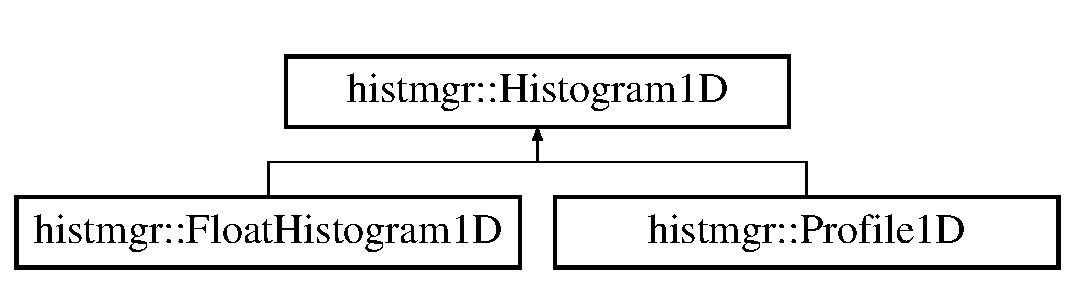
\includegraphics[height=2cm]{classhistmgr_1_1Histogram1D}
\end{center}
\end{figure}
\subsection*{Public Member Functions}
\begin{DoxyCompactItemize}
\item 
virtual int {\bf id} () const \label{classhistmgr_1_1Histogram1D_a524540a72e8d5f19fa3fcaec65610b0c}

\begin{DoxyCompactList}\small\item\em Return the id of the underlying LCGenericObjectImpl. \item\end{DoxyCompactList}\item 
UInt\_\-t {\bf firstBinIndex} () const \label{classhistmgr_1_1Histogram1D_acda829dea1a315f62e4618beecac3409}

\begin{DoxyCompactList}\small\item\em Return the index of the first bin not below the minimum axis value. \item\end{DoxyCompactList}\item 
UInt\_\-t {\bf lastBinIndex} () const \label{classhistmgr_1_1Histogram1D_a21cfe7d0e489202dcd0138da20349f74}

\begin{DoxyCompactList}\small\item\em Return the index of the last bin not above the maximum axis value. \item\end{DoxyCompactList}\item 
UInt\_\-t {\bf underflowBinIndex} () const \label{classhistmgr_1_1Histogram1D_a444200d12e95077d3ff93451ac9d51f5}

\begin{DoxyCompactList}\small\item\em Return the index of the bin below the minimum axis value (underflow bin). \item\end{DoxyCompactList}\item 
UInt\_\-t {\bf overflowBinIndex} () const \label{classhistmgr_1_1Histogram1D_a2f68dc59449bb4242e113cd62365acc7}

\begin{DoxyCompactList}\small\item\em Return the index of the bin above the maximum axis value (overflow bin). \item\end{DoxyCompactList}\item 
UInt\_\-t {\bf nBins} () const \label{classhistmgr_1_1Histogram1D_aabad63ec43eec6b9ec5250b409d50ef9}

\begin{DoxyCompactList}\small\item\em Return the number of bins. \item\end{DoxyCompactList}\item 
Float\_\-t {\bf xMin} () const \label{classhistmgr_1_1Histogram1D_a008b31ebefbd1149cc906975b7025996}

\begin{DoxyCompactList}\small\item\em The minimum axis value (lower edge of the histogram range). \item\end{DoxyCompactList}\item 
Float\_\-t {\bf xMax} () const \label{classhistmgr_1_1Histogram1D_aa1f98c2b6d73bcf1c0209f055d283c1b}

\begin{DoxyCompactList}\small\item\em The maximum axis value (upper edge of the histogram range). \item\end{DoxyCompactList}\item 
Float\_\-t {\bf binCenter} (UInt\_\-t bin\_\-index) const \label{classhistmgr_1_1Histogram1D_a74f37e72347aca0eb04085fe98b063da}

\begin{DoxyCompactList}\small\item\em Return the axis value of the centre of the given bin. \item\end{DoxyCompactList}\item 
Float\_\-t {\bfseries binLowEdge} (UInt\_\-t bin\_\-index) const \label{classhistmgr_1_1Histogram1D_a5cc5aa3eba6272c03a6147b860a8b8e3}

\item 
Float\_\-t {\bf binWidth} (UInt\_\-t) const \label{classhistmgr_1_1Histogram1D_a7c1fa00271d1776d054a8c337a56fd82}

\begin{DoxyCompactList}\small\item\em Return the width of the given bin. \item\end{DoxyCompactList}\item 
UInt\_\-t {\bf calice\_\-id} ()\label{classhistmgr_1_1Histogram1D_acd92f881bf13e97509720ddbb0063b4b}

\begin{DoxyCompactList}\small\item\em Return the id of the histogram. \item\end{DoxyCompactList}\item 
Double\_\-t {\bf entries} () const \label{classhistmgr_1_1Histogram1D_a22623460729f7e584282802d7320839c}

\begin{DoxyCompactList}\small\item\em Return the number of entries of the histogram. \item\end{DoxyCompactList}\end{DoxyCompactItemize}
\subsection*{Protected Member Functions}
\begin{DoxyCompactItemize}
\item 
{\bfseries Histogram1D} (lcio::LCObject $\ast$a\_\-obj)\label{classhistmgr_1_1Histogram1D_af17dcdb05c069e893c014c25581946ad}

\item 
void {\bf addToEntries} (Double\_\-t weight)
\begin{DoxyCompactList}\small\item\em Add weight to the number of entries. \item\end{DoxyCompactList}\item 
int {\bfseries getNInt} () const \label{classhistmgr_1_1Histogram1D_a9f6771b7dfedce460ba615330db8f3ee}

\item 
int {\bfseries getNFloat} () const \label{classhistmgr_1_1Histogram1D_a7df3b9136394f70dfe46e7465195134d}

\item 
int {\bfseries getNDouble} () const \label{classhistmgr_1_1Histogram1D_a40876551abee3a5cb68f7406024cb6fd}

\item 
int {\bfseries getIntVal} (int index) const \label{classhistmgr_1_1Histogram1D_a460737d4258f5bb33b2cda3a435c4fb6}

\item 
float {\bfseries getFloatVal} (int index) const \label{classhistmgr_1_1Histogram1D_a1a71d70f6c054b7cbab67ca04364f271}

\item 
double {\bfseries getDoubleVal} (int index) const \label{classhistmgr_1_1Histogram1D_a6e76a153525e974912e904a37c00c217}

\item 
bool {\bfseries isFixedSize} () const \label{classhistmgr_1_1Histogram1D_ae009c17abdb58995d8777a0ff4af75cd}

\item 
const std::string {\bfseries getTypeName} () const \label{classhistmgr_1_1Histogram1D_a89c9f20156c75f61297a5e4901e49936}

\item 
const std::string {\bfseries getDataDescription} () const \label{classhistmgr_1_1Histogram1D_aebfe652d6212c54e784489b13490853b}

\item 
void {\bf setBinning} (const {\bf HistPar} \&bins)\label{classhistmgr_1_1Histogram1D_aa8334230aef792b7cbec7dd4ff8e039b}

\begin{DoxyCompactList}\small\item\em Store the binning of the histogram. \item\end{DoxyCompactList}\item 
UInt\_\-t {\bf binIndex} (Float\_\-t value) const \label{classhistmgr_1_1Histogram1D_a42a8f19a46ae2582c1a913bc5c765831}

\begin{DoxyCompactList}\small\item\em Calculate and return the bin index for the given axis value. \item\end{DoxyCompactList}\item 
lcio::LCGenericObjectImpl $\ast$ {\bfseries obj} ()\label{classhistmgr_1_1Histogram1D_a87ce666baabddda16f4c1f22f57873d4}

\item 
const lcio::LCGenericObjectImpl $\ast$ {\bfseries obj} () const \label{classhistmgr_1_1Histogram1D_a2eea045a1d4a53f4ab193a93781bd3bf}

\end{DoxyCompactItemize}
\subsection*{Protected Attributes}
\begin{DoxyCompactItemize}
\item 
lcio::LCGenericObjectImpl $\ast$ {\bfseries \_\-obj}\label{classhistmgr_1_1Histogram1D_ac54ece569a39b15d5f29d685a08d161c}

\item 
bool {\bfseries \_\-createdObject}\label{classhistmgr_1_1Histogram1D_a4a49b47ef95c3733cd57cdc675227791}

\end{DoxyCompactItemize}
\subsection*{Static Protected Attributes}
\begin{DoxyCompactItemize}
\item 
static const std::string {\bfseries \_\-\_\-typeName} = \char`\"{}Histogram1D\char`\"{}\label{classhistmgr_1_1Histogram1D_a99612636650ea16a94249d8a068f3439}

\item 
static const std::string {\bfseries \_\-\_\-description} = \char`\"{}Histogram1D\char`\"{}\label{classhistmgr_1_1Histogram1D_aaa4194c1a6de8d9eb955a191edfd125c}

\end{DoxyCompactItemize}


\subsection{Detailed Description}
Equidistant binned 1D histogram without data container. The histogram is kept very simple and does not make use of virtual functions in order to be very fast. Note: the histogram does not have a data container. A usable histogram is the \doxyref{FloatHistogram1D}{p.}{classhistmgr_1_1FloatHistogram1D}. 

Definition at line 27 of file Histogram1D.hh.

\subsection{Member Function Documentation}
\index{histmgr::Histogram1D@{histmgr::Histogram1D}!addToEntries@{addToEntries}}
\index{addToEntries@{addToEntries}!histmgr::Histogram1D@{histmgr::Histogram1D}}
\subsubsection[{addToEntries}]{\setlength{\rightskip}{0pt plus 5cm}void histmgr::Histogram1D::addToEntries (Double\_\-t {\em weight})\hspace{0.3cm}{\ttfamily  [inline, protected]}}\label{classhistmgr_1_1Histogram1D_aa49e6a8526463293e4ca43c279ce3e86}


Add weight to the number of entries. Weight is usually 1, but may be a fractional value in the interval (0,oo). NOTE: No range check of the weight is performed. 

Definition at line 120 of file Histogram1D.hh.

References entries().

The documentation for this class was generated from the following files:\begin{DoxyCompactItemize}
\item 
Histogram1D.hh\item 
Histogram1D.cc\end{DoxyCompactItemize}

\section{histmgr::Histogram2D Class Reference}
\label{classhistmgr_1_1Histogram2D}\index{histmgr::Histogram2D@{histmgr::Histogram2D}}
Inheritance diagram for histmgr::Histogram2D::\begin{figure}[H]
\begin{center}
\leavevmode
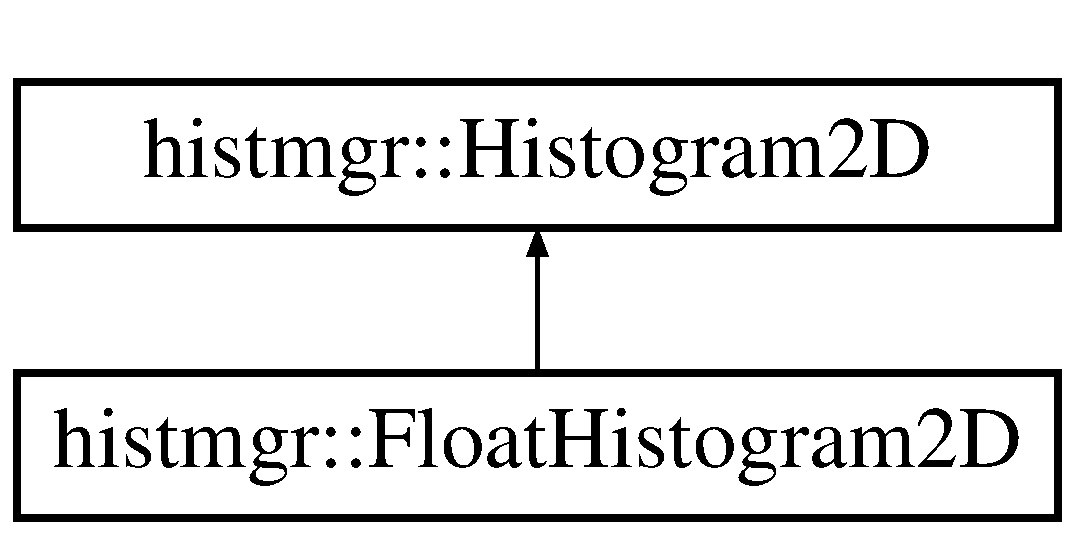
\includegraphics[height=2cm]{classhistmgr_1_1Histogram2D}
\end{center}
\end{figure}
\subsection*{Public Member Functions}
\begin{DoxyCompactItemize}
\item 
virtual int {\bf id} () const \label{classhistmgr_1_1Histogram2D_a76da2e4085a49feffbcf45457b55634d}

\begin{DoxyCompactList}\small\item\em Return the id of the underlying LCGenericObjectImpl. \item\end{DoxyCompactList}\item 
UInt\_\-t {\bfseries xFirstBinIndex} () const \label{classhistmgr_1_1Histogram2D_abf70969b4294719fb4c480d2485b6f02}

\item 
UInt\_\-t {\bfseries xLastBinIndex} () const \label{classhistmgr_1_1Histogram2D_aa816778d15e7eb3b9ab2affa02ceae0c}

\item 
UInt\_\-t {\bfseries yFirstBinIndex} () const \label{classhistmgr_1_1Histogram2D_a3e3a5b7d3d907c8be90ca562a2ea832c}

\item 
UInt\_\-t {\bfseries yLastBinIndex} () const \label{classhistmgr_1_1Histogram2D_af850544bb3c6d6a278e518a4ba7c5146}

\item 
UInt\_\-t {\bfseries xUnderflowBinIndex} () const \label{classhistmgr_1_1Histogram2D_ac6e27ddf89725fe49eeaf1568c8024c2}

\item 
UInt\_\-t {\bfseries xOverflowBinIndex} () const \label{classhistmgr_1_1Histogram2D_a6eb4490be5315d81c344a6e17d6cd1f6}

\item 
UInt\_\-t {\bfseries yUnderflowBinIndex} () const \label{classhistmgr_1_1Histogram2D_a09627b05e21e4544e621efc423936c81}

\item 
UInt\_\-t {\bfseries yOverflowBinIndex} () const \label{classhistmgr_1_1Histogram2D_a994f0c6eaf2179019ad0202282b73c80}

\item 
UInt\_\-t {\bfseries xNBins} () const \label{classhistmgr_1_1Histogram2D_a955bc09c119a9ccf995c40d055556250}

\item 
Float\_\-t {\bfseries xMin} () const \label{classhistmgr_1_1Histogram2D_a9c5990884d2b038d94e56640e8f70a12}

\item 
Float\_\-t {\bfseries xMax} () const \label{classhistmgr_1_1Histogram2D_a96a6a6d6dff2e8fe03a368c462c88952}

\item 
UInt\_\-t {\bfseries yNBins} () const \label{classhistmgr_1_1Histogram2D_a948a659fdd1a04946da319aacf809a75}

\item 
Float\_\-t {\bfseries yMin} () const \label{classhistmgr_1_1Histogram2D_acbe0f9156f69af35e7701796424efc57}

\item 
Float\_\-t {\bfseries yMax} () const \label{classhistmgr_1_1Histogram2D_a6e170388b9fe540e4553b2056691045d}

\item 
Float\_\-t {\bfseries xBinCenter} (UInt\_\-t bin\_\-index)\label{classhistmgr_1_1Histogram2D_a34240deb29b7af10792e82ab00a1ba96}

\item 
Float\_\-t {\bfseries xBinLowEdge} (UInt\_\-t bin\_\-index)\label{classhistmgr_1_1Histogram2D_a86e526af29aa24c0a0486f84d800fecf}

\item 
Float\_\-t {\bfseries xBinWidth} (UInt\_\-t)\label{classhistmgr_1_1Histogram2D_ac8fd83fa10fc3468361e4d2e56d50442}

\item 
Float\_\-t {\bfseries yBinCenter} (UInt\_\-t bin\_\-index)\label{classhistmgr_1_1Histogram2D_afed2edc77e0353c1366dc555f49e22c0}

\item 
Float\_\-t {\bfseries yBinLowEdge} (UInt\_\-t bin\_\-index)\label{classhistmgr_1_1Histogram2D_a3084d9ba1b47a865c36745fd19c7e7d3}

\item 
Float\_\-t {\bfseries yBinWidth} (UInt\_\-t)\label{classhistmgr_1_1Histogram2D_acc19b4a6e328acb6899de0c7504e2343}

\item 
UInt\_\-t {\bfseries calice\_\-id} ()\label{classhistmgr_1_1Histogram2D_aa6ea5c5bb5ff2b0fc7f6a8e9a5f3e625}

\item 
Double\_\-t {\bfseries entries} () const \label{classhistmgr_1_1Histogram2D_abb7d72e42edb6531399b10a91794382a}

\item 
void {\bfseries addToEntries} (Double\_\-t weight)\label{classhistmgr_1_1Histogram2D_a98f58e8e6d67a3430fb9047552c95b17}

\item 
int {\bfseries getNInt} () const \label{classhistmgr_1_1Histogram2D_a89e0f3cdde009efa4214734afb619960}

\item 
int {\bfseries getNFloat} () const \label{classhistmgr_1_1Histogram2D_acfe071923f9d990ec61568fd8c6e72f5}

\item 
int {\bfseries getNDouble} () const \label{classhistmgr_1_1Histogram2D_aa3292dae2356c865b67dc62fdd1abfb5}

\item 
int {\bfseries getIntVal} (int index) const \label{classhistmgr_1_1Histogram2D_a39f56d711ed8d5921f7662d038ead2d1}

\item 
float {\bfseries getFloatVal} (int index) const \label{classhistmgr_1_1Histogram2D_ab2fb60d75ad648ef7cdc259553a5c578}

\item 
double {\bfseries getDoubleVal} (int index) const \label{classhistmgr_1_1Histogram2D_a0ad3f76facb8a045e4ce6a0ac730e72a}

\item 
bool {\bfseries isFixedSize} () const \label{classhistmgr_1_1Histogram2D_a9062278e2daa5a095356fbf331b3b921}

\item 
const std::string {\bfseries getTypeName} () const \label{classhistmgr_1_1Histogram2D_aae1137af1c5d111b441b80d74ef606ba}

\item 
const std::string {\bfseries getDataDescription} () const \label{classhistmgr_1_1Histogram2D_aa9b8b32e5080f678d0b7e876c54ba453}

\end{DoxyCompactItemize}
\subsection*{Protected Member Functions}
\begin{DoxyCompactItemize}
\item 
{\bfseries Histogram2D} (lcio::LCObject $\ast$a\_\-obj)\label{classhistmgr_1_1Histogram2D_ade05eeddf75a2b5e341194c77fb9d101}

\item 
void {\bfseries setBinning} (const {\bf HistPar} \&x\_\-bins, const {\bf HistPar} \&y\_\-bins)\label{classhistmgr_1_1Histogram2D_a5599afe22a258e379309225ba43b8fd3}

\item 
void {\bfseries setXtoBins} ()\label{classhistmgr_1_1Histogram2D_a56dc039a37aa7bf88366e72e38535d9b}

\item 
void {\bfseries setYtoBins} ()\label{classhistmgr_1_1Histogram2D_adfafff46dede8944cb1a7569e864a1a2}

\item 
UInt\_\-t {\bfseries xBinIndex} (Float\_\-t value) const \label{classhistmgr_1_1Histogram2D_af1dab9a3f3ef0c7f015934014fbb6118}

\item 
UInt\_\-t {\bfseries yBinIndex} (Float\_\-t value) const \label{classhistmgr_1_1Histogram2D_abc60652d0255c12f81b5ac270f28e744}

\item 
UInt\_\-t {\bfseries getContainerSize} () const \label{classhistmgr_1_1Histogram2D_adc5826e91c1e1b571fb9a1a0c3cbdadf}

\item 
lcio::LCGenericObjectImpl $\ast$ {\bfseries obj} ()\label{classhistmgr_1_1Histogram2D_a858dc3152e69254166a94bd9da833be3}

\item 
const lcio::LCGenericObjectImpl $\ast$ {\bfseries obj} () const \label{classhistmgr_1_1Histogram2D_a727d937e500b3a05a8c1d9d197198bfb}

\end{DoxyCompactItemize}
\subsection*{Protected Attributes}
\begin{DoxyCompactItemize}
\item 
lcio::LCGenericObjectImpl $\ast$ {\bfseries \_\-obj}\label{classhistmgr_1_1Histogram2D_ac665536e5e1b13a7482018306b70424d}

\item 
bool {\bfseries \_\-createdObject}\label{classhistmgr_1_1Histogram2D_a5e72c0d4241393ceda4f54a441cc9d72}

\item 
Double\_\-t {\bfseries \_\-xToBin}\label{classhistmgr_1_1Histogram2D_aee7de840bafcc507ff2cf1165ad97c53}

\item 
Double\_\-t {\bfseries \_\-yToBin}\label{classhistmgr_1_1Histogram2D_af65c161601e9290bc97be2f8debbecd8}

\end{DoxyCompactItemize}
\subsection*{Static Protected Attributes}
\begin{DoxyCompactItemize}
\item 
static const std::string {\bfseries \_\-\_\-typeName} = \char`\"{}Histogram2D\char`\"{}\label{classhistmgr_1_1Histogram2D_ae180a84a85576bfe6648db62f402d42e}

\item 
static const std::string {\bfseries \_\-\_\-description} = \char`\"{}Histogram2D\char`\"{}\label{classhistmgr_1_1Histogram2D_a0d54044cca0f5111309d9a22481b6236}

\end{DoxyCompactItemize}


\subsection{Detailed Description}


Definition at line 22 of file Histogram2D.hh.

The documentation for this class was generated from the following files:\begin{DoxyCompactItemize}
\item 
Histogram2D.hh\item 
Histogram2D.cc\end{DoxyCompactItemize}

\section{histmgr::Histogram2DCollection\_\-t Class Reference}
\label{classhistmgr_1_1Histogram2DCollection__t}\index{histmgr::Histogram2DCollection\_\-t@{histmgr::Histogram2DCollection\_\-t}}


One or two dimensional collection of histograms.  


{\ttfamily \#include $<$Histogram2DCollection\_\-t.hh$>$}Inheritance diagram for histmgr::Histogram2DCollection\_\-t::\begin{figure}[H]
\begin{center}
\leavevmode
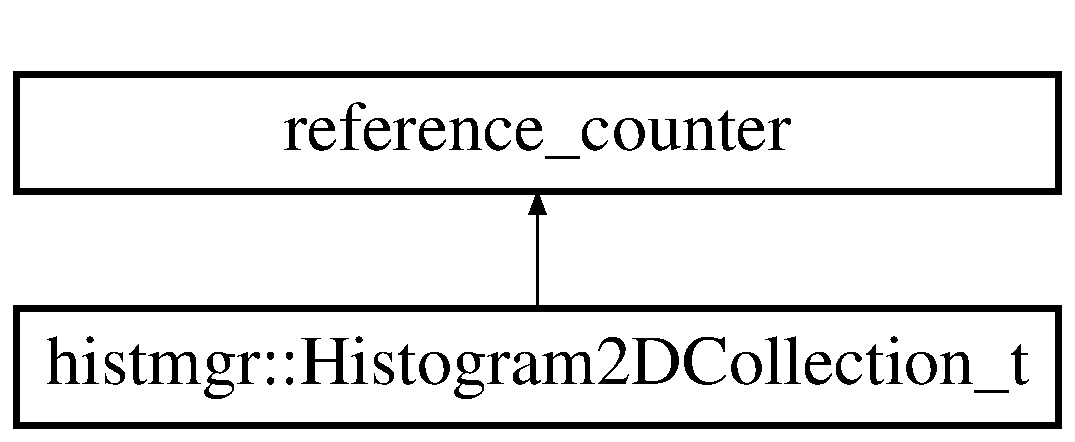
\includegraphics[height=2cm]{classhistmgr_1_1Histogram2DCollection__t}
\end{center}
\end{figure}
\subsection*{Public Member Functions}
\begin{DoxyCompactItemize}
\item 
{\bf Histogram2DCollection\_\-t} (const std::string \&collection\_\-name, const EVENT::StringVec \&name\_\-list, UInt\_\-t n\_\-hist, const {\bf HistPar} \&x\_\-par, const {\bf HistPar} \&y\_\-par)  throw (std::bad\_\-alloc, std::runtime\_\-error)
\begin{DoxyCompactList}\small\item\em Create a collection of histograms which will have the same binning and the same name (except of a numeric extension). \item\end{DoxyCompactList}\item 
{\bf Histogram2DCollection\_\-t} (const std::string \&collection\_\-name, const EVENT::StringVec \&name\_\-list, const lcio::IntVec \&n\_\-hist\_\-list, const {\bf HistPar} \&x\_\-par, const {\bf HistPar} \&y\_\-par)
\begin{DoxyCompactList}\small\item\em Create a collection of histograms which will have the same binning and the same name (except of a numeric extension). \item\end{DoxyCompactList}\item 
{\bf Histogram2DCollection\_\-t} (lcio::LCCollection $\ast$histograms, lcio::IntVec $\ast$indices)
\item 
{\bf Histogram2DCollection\_\-t} (lcio::LCCollection $\ast$histograms)
\begin{DoxyCompactList}\small\item\em Create a histogram collection from lcio collection. \item\end{DoxyCompactList}\item 
{\bf Histogram2DCollection\_\-t} (const {\bf Histogram2DCollection\_\-t} \&a)\label{classhistmgr_1_1Histogram2DCollection__t_a2f6e961d72d471440615a4673d3f2de4}

\begin{DoxyCompactList}\small\item\em copy constructor. \item\end{DoxyCompactList}\item 
{\bf Histogram2DCollection\_\-t} ()\label{classhistmgr_1_1Histogram2DCollection__t_aa51815c63839cc73273232df3cc53d91}

\begin{DoxyCompactList}\small\item\em Default constructor. \item\end{DoxyCompactList}\item 
void {\bf deleteCollection} ()\label{classhistmgr_1_1Histogram2DCollection__t_a3dc0a213db50d0a0eb58441ce29875c6}

\begin{DoxyCompactList}\small\item\em delete the histogram collection and the index array This method exists instead of a destrctor to prevent copying the arrays (FIXME) \item\end{DoxyCompactList}\item 
void {\bfseries deleteSharedStorage} ()\label{classhistmgr_1_1Histogram2DCollection__t_aa8f4d87ede0c6bbcc3f22cea2dca2f3f}

\item 
lcio::LCCollection $\ast$ {\bf createHistograms} (const std::string \&collection\_\-name, const EVENT::StringVec \&name\_\-list, UInt\_\-t n\_\-hist, const {\bf HistPar} \&x\_\-par, const {\bf HistPar} \&y\_\-par)  throw (std::bad\_\-alloc,std::runtime\_\-error)
\begin{DoxyCompactList}\small\item\em create several histograms which will have the same binning and the same name (except of a numeric extension). \item\end{DoxyCompactList}\item 
lcio::LCCollection $\ast$ {\bf createHistograms} (const std::string \&collection\_\-name, const EVENT::StringVec \&name\_\-list, const lcio::IntVec \&n\_\-hist\_\-list, const {\bf HistPar} \&x\_\-par, const {\bf HistPar} \&y\_\-par)  throw (std::bad\_\-alloc,std::runtime\_\-error)
\begin{DoxyCompactList}\small\item\em create several histograms which will have the same binning and the same name (except of a numeric extension). \item\end{DoxyCompactList}\item 
lcio::LCCollection $\ast$ {\bf collection} ()
\begin{DoxyCompactList}\small\item\em get the unique group id \item\end{DoxyCompactList}\item 
const lcio::LCCollection $\ast$ {\bf collection} () const 
\begin{DoxyCompactList}\small\item\em get the collection of histograms (read only). \item\end{DoxyCompactList}\item 
UInt\_\-t {\bf n} () const \label{classhistmgr_1_1Histogram2DCollection__t_a4aa15bd76ec1a055afe867e0a59daab6}

\begin{DoxyCompactList}\small\item\em get the number of histograms in the one dimensional collection. \item\end{DoxyCompactList}\item 
bool {\bf is2D} () const \label{classhistmgr_1_1Histogram2DCollection__t_a915231d0006aa618929865be0717d676}

\begin{DoxyCompactList}\small\item\em Return true if the histogram collection is two instead of one diemensional. \item\end{DoxyCompactList}\item 
UInt\_\-t {\bf nMajor} () const \label{classhistmgr_1_1Histogram2DCollection__t_a7d589f32e849ee6c2ff62d22f67e596b}

\begin{DoxyCompactList}\small\item\em get the number of histograms in the one dimensional collection. \item\end{DoxyCompactList}\item 
UInt\_\-t {\bf nMinor} (UInt\_\-t major\_\-index) const \label{classhistmgr_1_1Histogram2DCollection__t_af72ed2b8399f39439bc2b232820696f2}

\begin{DoxyCompactList}\small\item\em get the number of histograms in the one dimensional collection. \item\end{DoxyCompactList}\item 
const {\bf FloatHistogram2D} $\ast$ {\bf histogram} (UInt\_\-t index) const \label{classhistmgr_1_1Histogram2DCollection__t_abd1f0ccdbc83f9f6fbbea239162d99d8}

\begin{DoxyCompactList}\small\item\em Get one histogram of the collection (read only). \item\end{DoxyCompactList}\item 
{\bf FloatHistogram2D} $\ast$ {\bf histogram} (UInt\_\-t index)\label{classhistmgr_1_1Histogram2DCollection__t_afc8d2ea4e42d5e6cf283792b819d95c1}

\begin{DoxyCompactList}\small\item\em Get one histogram of the collection. \item\end{DoxyCompactList}\item 
{\bf FloatHistogram2D} $\ast$ {\bf histogram} (UInt\_\-t major\_\-index, UInt\_\-t minor\_\-index)\label{classhistmgr_1_1Histogram2DCollection__t_a182a4f9dd876337a00a5e57f8358555f}

\begin{DoxyCompactList}\small\item\em Get one histogram of the collection which is organised as a two dimensional array. \item\end{DoxyCompactList}\item 
const {\bf FloatHistogram2D} $\ast$ {\bf histogram} (UInt\_\-t major\_\-index, UInt\_\-t minor\_\-index) const \label{classhistmgr_1_1Histogram2DCollection__t_a3ea359f9713ea66fe5ceaf0b82539776}

\begin{DoxyCompactList}\small\item\em Get one histogram of the collection which is organised as a two dimensional array (read only). \item\end{DoxyCompactList}\item 
const std::string \& {\bf getName} (UInt\_\-t major\_\-index) const 
\begin{DoxyCompactList}\small\item\em Get the name of the specified element of the histogram collection. \item\end{DoxyCompactList}\end{DoxyCompactItemize}
\subsection*{Static Protected Attributes}
\begin{DoxyCompactItemize}
\item 
static const std::string {\bfseries \_\-\_\-histogramNameParameterName}\label{classhistmgr_1_1Histogram2DCollection__t_a9c9c12ef5e660181a010b4e9e3543e8d}

\end{DoxyCompactItemize}
\subsection*{Private Member Functions}
\begin{DoxyCompactItemize}
\item 
void {\bf copyNames} () const 
\begin{DoxyCompactList}\small\item\em Copy the names from the collection to an accessible vector. \item\end{DoxyCompactList}\end{DoxyCompactItemize}
\subsection*{Private Attributes}
\begin{DoxyCompactItemize}
\item 
lcio::LCCollection $\ast$ {\bf \_\-histogramCol}\label{classhistmgr_1_1Histogram2DCollection__t_a935072d41133e1922cfa3372a859bda8}

\begin{DoxyCompactList}\small\item\em the histogram collection \item\end{DoxyCompactList}\item 
lcio::IntVec $\ast$ {\bf \_\-majorIndex}
\begin{DoxyCompactList}\small\item\em optional list of offset to form a two dimensional array out of the list. \item\end{DoxyCompactList}\item 
lcio::StringVec {\bf \_\-nameList}
\begin{DoxyCompactList}\small\item\em A vector which contains one name for all histograms of the collection or a name for each element. \item\end{DoxyCompactList}\end{DoxyCompactItemize}
\subsection*{Static Private Attributes}
\begin{DoxyCompactItemize}
\item 
static const std::string {\bfseries \_\-\_\-majorIndexParameterName}\label{classhistmgr_1_1Histogram2DCollection__t_aded8e87a24b7ee1bd042c0bb352fdf1d}

\item 
static const std::string {\bfseries \_\-\_\-defaultHistogramName}\label{classhistmgr_1_1Histogram2DCollection__t_ac482b686014b906aa2be8da6a4ca9844}

\end{DoxyCompactItemize}
\subsection*{Friends}
\begin{DoxyCompactItemize}
\item 
class {\bfseries HistMgr}\label{classhistmgr_1_1Histogram2DCollection__t_a3cc85db784d7651390e41024125eb3a0}

\end{DoxyCompactItemize}


\subsection{Detailed Description}
One or two dimensional collection of histograms. 

Definition at line 16 of file Histogram2DCollection\_\-t.hh.

\subsection{Constructor \& Destructor Documentation}
\index{histmgr::Histogram2DCollection\_\-t@{histmgr::Histogram2DCollection\_\-t}!Histogram2DCollection\_\-t@{Histogram2DCollection\_\-t}}
\index{Histogram2DCollection\_\-t@{Histogram2DCollection\_\-t}!histmgr::Histogram2DCollection_t@{histmgr::Histogram2DCollection\_\-t}}
\subsubsection[{Histogram2DCollection\_\-t}]{\setlength{\rightskip}{0pt plus 5cm}histmgr::Histogram2DCollection\_\-t::Histogram2DCollection\_\-t (const std::string \& {\em collection\_\-name}, \/  const EVENT::StringVec \& {\em name\_\-list}, \/  UInt\_\-t {\em n\_\-hist}, \/  const {\bf HistPar} \& {\em x\_\-par}, \/  const {\bf HistPar} \& {\em y\_\-par})  throw (std::bad\_\-alloc, std::runtime\_\-error)\hspace{0.3cm}{\ttfamily  [inline]}}\label{classhistmgr_1_1Histogram2DCollection__t_a35a0952578e1a6df03a4582455e5a168}


Create a collection of histograms which will have the same binning and the same name (except of a numeric extension). 
\begin{DoxyParams}{Parameters}
\item[{\em collection\_\-name}]the name of the histogram collection \item[{\em name\_\-list}]a vector containing the names of the histograms whose length is either equals n\_\-hist or is zero. In the latter case the collection name is used for the all histograms. \item[{\em n\_\-hist}]the number of histograms to be created \item[{\em x\_\-par}]the binning of the x-\/axis of the histogram \item[{\em y\_\-par}]the binning of the y-\/axis of the histogram\end{DoxyParams}
The histograms are only written to a file if the histogram group, to which this histogram belongs, is assigned to a file (\doxyref{histmgr::HistMgr::assignFileName}{p.}{classhistmgr_1_1HistMgr_a20e3c96a8ba6175c8036918ca7acb1e2}). 

Definition at line 33 of file Histogram2DCollection\_\-t.hh.

References createHistograms().\index{histmgr::Histogram2DCollection\_\-t@{histmgr::Histogram2DCollection\_\-t}!Histogram2DCollection\_\-t@{Histogram2DCollection\_\-t}}
\index{Histogram2DCollection\_\-t@{Histogram2DCollection\_\-t}!histmgr::Histogram2DCollection_t@{histmgr::Histogram2DCollection\_\-t}}
\subsubsection[{Histogram2DCollection\_\-t}]{\setlength{\rightskip}{0pt plus 5cm}histmgr::Histogram2DCollection\_\-t::Histogram2DCollection\_\-t (const std::string \& {\em collection\_\-name}, \/  const EVENT::StringVec \& {\em name\_\-list}, \/  const lcio::IntVec \& {\em n\_\-hist\_\-list}, \/  const {\bf HistPar} \& {\em x\_\-par}, \/  const {\bf HistPar} \& {\em y\_\-par})\hspace{0.3cm}{\ttfamily  [inline]}}\label{classhistmgr_1_1Histogram2DCollection__t_a787b3b7485747847457337b7e138f0ed}


Create a collection of histograms which will have the same binning and the same name (except of a numeric extension). 
\begin{DoxyParams}{Parameters}
\item[{\em collection\_\-name}]the of the histogram collection \item[{\em name\_\-list}]a vector containing the names of the histograms whose length is either equals n\_\-hist or is zero. In the latter case the collection name is used for the all histograms. \item[{\em n\_\-hist\_\-list}]the number of histograms to be created \item[{\em x\_\-par}]the binning of the x-\/axis of the histogram \item[{\em y\_\-par}]the binning of the y-\/axis of the histogram\end{DoxyParams}
\begin{DoxyReturn}{Returns}
pointer to the histogram collection
\end{DoxyReturn}
The histograms are only written to a file if the histogram group, to which this histogram belongs, is assigned to a file (\doxyref{histmgr::HistMgr::assignFileName}{p.}{classhistmgr_1_1HistMgr_a20e3c96a8ba6175c8036918ca7acb1e2}). 

Definition at line 60 of file Histogram2DCollection\_\-t.hh.

References createHistograms().\index{histmgr::Histogram2DCollection\_\-t@{histmgr::Histogram2DCollection\_\-t}!Histogram2DCollection\_\-t@{Histogram2DCollection\_\-t}}
\index{Histogram2DCollection\_\-t@{Histogram2DCollection\_\-t}!histmgr::Histogram2DCollection_t@{histmgr::Histogram2DCollection\_\-t}}
\subsubsection[{Histogram2DCollection\_\-t}]{\setlength{\rightskip}{0pt plus 5cm}histmgr::Histogram2DCollection\_\-t::Histogram2DCollection\_\-t (lcio::LCCollection $\ast$ {\em histograms}, \/  lcio::IntVec $\ast$ {\em indices})\hspace{0.3cm}{\ttfamily  [inline]}}\label{classhistmgr_1_1Histogram2DCollection__t_adb283f18b76bde0d93371c93e2ab372d}

\begin{DoxyParams}{Parameters}
\item[{\em histograms}]the linearised one or two dimensional collection of histograms \item[{\em indices}]optional list of indicies used to give two dimensional access to the histogram list. for each possible index of the first dimension is needed which contains the offset in the list. The second index is added to this offset. \end{DoxyParams}


Definition at line 78 of file Histogram2DCollection\_\-t.hh.

References \_\-majorIndex.\index{histmgr::Histogram2DCollection\_\-t@{histmgr::Histogram2DCollection\_\-t}!Histogram2DCollection\_\-t@{Histogram2DCollection\_\-t}}
\index{Histogram2DCollection\_\-t@{Histogram2DCollection\_\-t}!histmgr::Histogram2DCollection_t@{histmgr::Histogram2DCollection\_\-t}}
\subsubsection[{Histogram2DCollection\_\-t}]{\setlength{\rightskip}{0pt plus 5cm}histmgr::Histogram2DCollection\_\-t::Histogram2DCollection\_\-t (lcio::LCCollection $\ast$ {\em histograms})\hspace{0.3cm}{\ttfamily  [inline]}}\label{classhistmgr_1_1Histogram2DCollection__t_a0f2cfcb743a248e92180d3b852706ac8}


Create a histogram collection from lcio collection. 
\begin{DoxyParams}{Parameters}
\item[{\em histograms}]the linearised one or two dimensional collection of histograms (two dimensional collections have the collection parameter \char`\"{}major\char`\"{}). The method does not verify whether the lcio collection really is a histogram collection. However, if the collection has the parameter \char`\"{}major\char`\"{} it creates an index vector (costly operation) assuming that it is a 2d array instead of a 1d array(i.e. collection). The unique group id remains undedfined since it is not stored in the lcio collection. \end{DoxyParams}


Definition at line 105 of file Histogram2DCollection\_\-t.hh.

References \_\-majorIndex.

\subsection{Member Function Documentation}
\index{histmgr::Histogram2DCollection\_\-t@{histmgr::Histogram2DCollection\_\-t}!collection@{collection}}
\index{collection@{collection}!histmgr::Histogram2DCollection_t@{histmgr::Histogram2DCollection\_\-t}}
\subsubsection[{collection}]{\setlength{\rightskip}{0pt plus 5cm}const lcio::LCCollection$\ast$ histmgr::Histogram2DCollection\_\-t::collection () const\hspace{0.3cm}{\ttfamily  [inline]}}\label{classhistmgr_1_1Histogram2DCollection__t_a17fbf5af12ce7ab4173bf35eab2f5605}


get the collection of histograms (read only). The index array needed for the two dimensional acces is added as a parameter named \char`\"{}major\char`\"{}. 

Definition at line 214 of file Histogram2DCollection\_\-t.hh.

References \_\-histogramCol.\index{histmgr::Histogram2DCollection\_\-t@{histmgr::Histogram2DCollection\_\-t}!collection@{collection}}
\index{collection@{collection}!histmgr::Histogram2DCollection_t@{histmgr::Histogram2DCollection\_\-t}}
\subsubsection[{collection}]{\setlength{\rightskip}{0pt plus 5cm}lcio::LCCollection$\ast$ histmgr::Histogram2DCollection\_\-t::collection ()\hspace{0.3cm}{\ttfamily  [inline]}}\label{classhistmgr_1_1Histogram2DCollection__t_a188140d679c38c1f48a44e0415dabbd6}


get the unique group id get the collection of histograms. The index array needed for the two dimensional acces is added as a parameter named \char`\"{}major\char`\"{}. 

Definition at line 209 of file Histogram2DCollection\_\-t.hh.

References \_\-histogramCol.\index{histmgr::Histogram2DCollection\_\-t@{histmgr::Histogram2DCollection\_\-t}!copyNames@{copyNames}}
\index{copyNames@{copyNames}!histmgr::Histogram2DCollection_t@{histmgr::Histogram2DCollection\_\-t}}
\subsubsection[{copyNames}]{\setlength{\rightskip}{0pt plus 5cm}void histmgr::Histogram2DCollection\_\-t::copyNames () const\hspace{0.3cm}{\ttfamily  [inline, private]}}\label{classhistmgr_1_1Histogram2DCollection__t_a4dd304e748d23c5f5deba573e1071356}


Copy the names from the collection to an accessible vector. The vector of histogram names is attached as a parameter to the LCCollection. 

Definition at line 362 of file Histogram2DCollection\_\-t.hh.

References \_\-histogramCol, and \_\-nameList.

Referenced by getName().\index{histmgr::Histogram2DCollection\_\-t@{histmgr::Histogram2DCollection\_\-t}!createHistograms@{createHistograms}}
\index{createHistograms@{createHistograms}!histmgr::Histogram2DCollection_t@{histmgr::Histogram2DCollection\_\-t}}
\subsubsection[{createHistograms}]{\setlength{\rightskip}{0pt plus 5cm}lcio::LCCollection $\ast$ histmgr::Histogram2DCollection\_\-t::createHistograms (const std::string \& {\em collection\_\-name}, \/  const EVENT::StringVec \& {\em name\_\-list}, \/  const lcio::IntVec \& {\em n\_\-hist\_\-list}, \/  const {\bf HistPar} \& {\em x\_\-par}, \/  const {\bf HistPar} \& {\em y\_\-par})  throw (std::bad\_\-alloc,std::runtime\_\-error)}\label{classhistmgr_1_1Histogram2DCollection__t_abff52f3851380b23b55dc311345fb400}


create several histograms which will have the same binning and the same name (except of a numeric extension). 
\begin{DoxyParams}{Parameters}
\item[{\em collection\_\-name}]the of the histogram collection \item[{\em name\_\-list}]a vector containing the names of the histograms whose length is either equals n\_\-hist or is zero. In the latter case the collection name is used for the all histograms. \item[{\em n\_\-hist\_\-list}]the number of histograms to be created \item[{\em x\_\-par}]the binning of the x-\/axis of the histogram \item[{\em y\_\-par}]the binning of the y-\/axis of the histogram\end{DoxyParams}
\begin{DoxyReturn}{Returns}
pointer to the histogram collection
\end{DoxyReturn}
The histograms are only written to a file if the histogram group, to which this histogram belongs, is assigned to a file (\doxyref{histmgr::HistMgr::assignFileName}{p.}{classhistmgr_1_1HistMgr_a20e3c96a8ba6175c8036918ca7acb1e2}). 

Definition at line 70 of file Histogram2DCollection\_\-t.cc.\index{histmgr::Histogram2DCollection\_\-t@{histmgr::Histogram2DCollection\_\-t}!createHistograms@{createHistograms}}
\index{createHistograms@{createHistograms}!histmgr::Histogram2DCollection_t@{histmgr::Histogram2DCollection\_\-t}}
\subsubsection[{createHistograms}]{\setlength{\rightskip}{0pt plus 5cm}lcio::LCCollection $\ast$ histmgr::Histogram2DCollection\_\-t::createHistograms (const std::string \& {\em collection\_\-name}, \/  const EVENT::StringVec \& {\em name\_\-list}, \/  UInt\_\-t {\em n\_\-hist}, \/  const {\bf HistPar} \& {\em x\_\-par}, \/  const {\bf HistPar} \& {\em y\_\-par})  throw (std::bad\_\-alloc,std::runtime\_\-error)}\label{classhistmgr_1_1Histogram2DCollection__t_a3ee9c9b75d9b166ebb894a5ef232862f}


create several histograms which will have the same binning and the same name (except of a numeric extension). 
\begin{DoxyParams}{Parameters}
\item[{\em collection\_\-name}]the of the histogram collection \item[{\em name\_\-list}]a vector containing the names of the histograms whose length is either equals n\_\-hist or is zero. In the latter case the collection name is used for the all histograms. \item[{\em n\_\-hist}]the number of histograms to be created \item[{\em x\_\-par}]the binning of the x-\/axis of the histogram \item[{\em y\_\-par}]the binning of the y-\/axis of the histogram\end{DoxyParams}
\begin{DoxyReturn}{Returns}
pointer to the histogram collection.
\end{DoxyReturn}
The histograms are only written to a file if the histogram group, to which this histogram belongs, is assigned to a file (\doxyref{histmgr::HistMgr::assignFileName}{p.}{classhistmgr_1_1HistMgr_a20e3c96a8ba6175c8036918ca7acb1e2}). 

Definition at line 16 of file Histogram2DCollection\_\-t.cc.

Referenced by Histogram2DCollection\_\-t().\index{histmgr::Histogram2DCollection\_\-t@{histmgr::Histogram2DCollection\_\-t}!getName@{getName}}
\index{getName@{getName}!histmgr::Histogram2DCollection_t@{histmgr::Histogram2DCollection\_\-t}}
\subsubsection[{getName}]{\setlength{\rightskip}{0pt plus 5cm}const std::string\& histmgr::Histogram2DCollection\_\-t::getName (UInt\_\-t {\em major\_\-index}) const\hspace{0.3cm}{\ttfamily  [inline]}}\label{classhistmgr_1_1Histogram2DCollection__t_af3b3d5ea47b48bade82960964d812f81}


Get the name of the specified element of the histogram collection. 
\begin{DoxyParams}{Parameters}
\item[{\em major\_\-index}]the index of the histogram element or in case of an 2D histogram array the major index. \end{DoxyParams}
\begin{DoxyReturn}{Returns}
a reference to the name. 
\end{DoxyReturn}


Definition at line 332 of file Histogram2DCollection\_\-t.hh.

References \_\-nameList, and copyNames().

\subsection{Field Documentation}
\index{histmgr::Histogram2DCollection\_\-t@{histmgr::Histogram2DCollection\_\-t}!\_\-majorIndex@{\_\-majorIndex}}
\index{\_\-majorIndex@{\_\-majorIndex}!histmgr::Histogram2DCollection_t@{histmgr::Histogram2DCollection\_\-t}}
\subsubsection[{\_\-majorIndex}]{\setlength{\rightskip}{0pt plus 5cm}lcio::IntVec$\ast$ {\bf histmgr::Histogram2DCollection\_\-t::\_\-majorIndex}\hspace{0.3cm}{\ttfamily  [private]}}\label{classhistmgr_1_1Histogram2DCollection__t_a5cf6937dc68176cb4d65e424ed566acb}


optional list of offset to form a two dimensional array out of the list. 

Definition at line 373 of file Histogram2DCollection\_\-t.hh.

Referenced by deleteCollection(), histogram(), Histogram2DCollection\_\-t(), is2D(), nMajor(), and nMinor().\index{histmgr::Histogram2DCollection\_\-t@{histmgr::Histogram2DCollection\_\-t}!\_\-nameList@{\_\-nameList}}
\index{\_\-nameList@{\_\-nameList}!histmgr::Histogram2DCollection_t@{histmgr::Histogram2DCollection\_\-t}}
\subsubsection[{\_\-nameList}]{\setlength{\rightskip}{0pt plus 5cm}lcio::StringVec {\bf histmgr::Histogram2DCollection\_\-t::\_\-nameList}\hspace{0.3cm}{\ttfamily  [mutable, private]}}\label{classhistmgr_1_1Histogram2DCollection__t_a1de57f0f5cb991d9355792fed7faa639}


A vector which contains one name for all histograms of the collection or a name for each element. 

Definition at line 375 of file Histogram2DCollection\_\-t.hh.

Referenced by copyNames(), and getName().

The documentation for this class was generated from the following files:\begin{DoxyCompactItemize}
\item 
Histogram2DCollection\_\-t.hh\item 
Histogram2DCollection\_\-t.cc\end{DoxyCompactItemize}

\section{histmgr::HistogramCollection\_\-t Class Reference}
\label{classhistmgr_1_1HistogramCollection__t}\index{histmgr::HistogramCollection\_\-t@{histmgr::HistogramCollection\_\-t}}


One or two dimensional collection of histograms.  


{\ttfamily \#include $<$HistogramCollection\_\-t.hh$>$}Inheritance diagram for histmgr::HistogramCollection\_\-t::\begin{figure}[H]
\begin{center}
\leavevmode
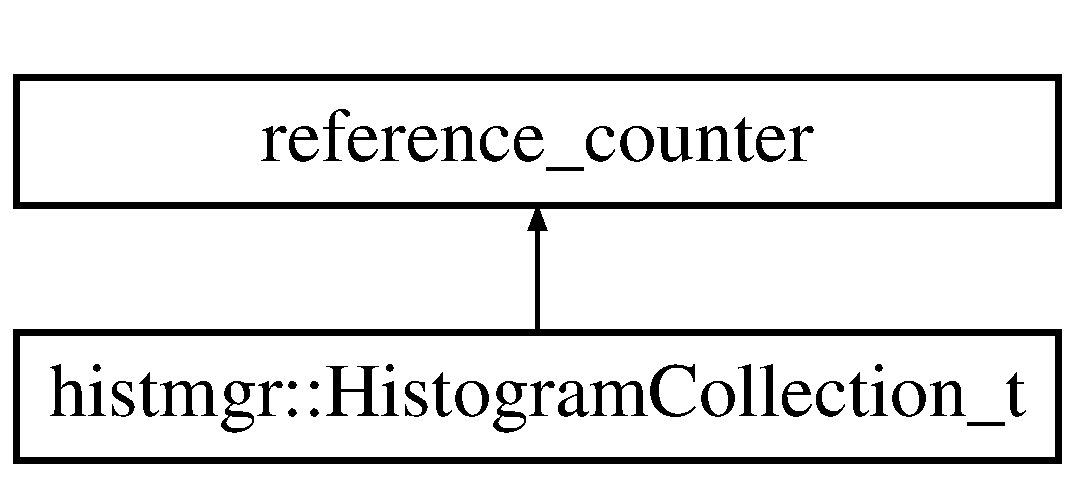
\includegraphics[height=2cm]{classhistmgr_1_1HistogramCollection__t}
\end{center}
\end{figure}
\subsection*{Public Member Functions}
\begin{DoxyCompactItemize}
\item 
{\bf HistogramCollection\_\-t} (const std::string \&collection\_\-name, const EVENT::StringVec \&name\_\-list, UInt\_\-t n\_\-hist, const {\bf HistPar} \&par)  throw (std::bad\_\-alloc, std::runtime\_\-error)
\begin{DoxyCompactList}\small\item\em Create a collection of histograms which will have the same binning and the same name (except of a numeric extension). \item\end{DoxyCompactList}\item 
{\bf HistogramCollection\_\-t} (const std::string \&collection\_\-name, const EVENT::StringVec \&name\_\-list, const lcio::IntVec \&n\_\-hist\_\-list, const {\bf HistPar} \&par)
\begin{DoxyCompactList}\small\item\em Create a collection of histograms which will have the same binning and the same name (except of a numeric extension). \item\end{DoxyCompactList}\item 
{\bf HistogramCollection\_\-t} (lcio::LCCollection $\ast$histograms, lcio::IntVec $\ast$indices)
\item 
{\bf HistogramCollection\_\-t} (lcio::LCCollection $\ast$histograms)
\begin{DoxyCompactList}\small\item\em Create a histogram collection from lcio collection. \item\end{DoxyCompactList}\item 
{\bf HistogramCollection\_\-t} (const {\bf HistogramCollection\_\-t} \&a)\label{classhistmgr_1_1HistogramCollection__t_a2021dd1769b2d44df3a2c21fd9cec651}

\begin{DoxyCompactList}\small\item\em copy constructor. \item\end{DoxyCompactList}\item 
{\bf HistogramCollection\_\-t} ()\label{classhistmgr_1_1HistogramCollection__t_a707cc7dfca722efaf6c4fd1bd5edaf16}

\begin{DoxyCompactList}\small\item\em Default constructor. \item\end{DoxyCompactList}\item 
void {\bf deleteCollection} ()\label{classhistmgr_1_1HistogramCollection__t_aab14375abc9104cae8cd1e244155b95e}

\begin{DoxyCompactList}\small\item\em delete the histogram collection and the index array This method exists instead of a destrctor to prevent copying the arrays (FIXME) \item\end{DoxyCompactList}\item 
void {\bfseries deleteSharedStorage} ()\label{classhistmgr_1_1HistogramCollection__t_ac9c1e7058781ce12c5409ea6aacea91d}

\item 
lcio::LCCollection $\ast$ {\bf createHistograms} (const std::string \&collection\_\-name, const EVENT::StringVec \&name\_\-list, UInt\_\-t n\_\-hist, const {\bf HistPar} \&par)  throw (std::bad\_\-alloc,std::runtime\_\-error)
\begin{DoxyCompactList}\small\item\em create several histograms which will have the same binning and the same name (except of a numeric extension). \item\end{DoxyCompactList}\item 
lcio::LCCollection $\ast$ {\bf createHistograms} (const std::string \&collection\_\-name, const EVENT::StringVec \&name\_\-list, const lcio::IntVec \&n\_\-hist\_\-list, const {\bf HistPar} \&par)  throw (std::bad\_\-alloc,std::runtime\_\-error)
\begin{DoxyCompactList}\small\item\em create several histograms which will have the same binning and the same name (except of a numeric extension). \item\end{DoxyCompactList}\item 
lcio::LCCollection $\ast$ {\bf collection} ()
\begin{DoxyCompactList}\small\item\em get the unique group id \item\end{DoxyCompactList}\item 
const lcio::LCCollection $\ast$ {\bf collection} () const 
\begin{DoxyCompactList}\small\item\em get the collection of histograms (read only). \item\end{DoxyCompactList}\item 
UInt\_\-t {\bf n} () const \label{classhistmgr_1_1HistogramCollection__t_ac42b746ee1dbd26e5860e92ba1e473ec}

\begin{DoxyCompactList}\small\item\em get the number of histograms in the one dimensional collection. \item\end{DoxyCompactList}\item 
bool {\bf is2D} () const \label{classhistmgr_1_1HistogramCollection__t_a559133040ee3b0194f15c2c957305798}

\begin{DoxyCompactList}\small\item\em Return true if the histogram collection is two instead of one diemensional. \item\end{DoxyCompactList}\item 
UInt\_\-t {\bf nMajor} () const \label{classhistmgr_1_1HistogramCollection__t_a02818178f9b34adc8fc34077f1111ae0}

\begin{DoxyCompactList}\small\item\em get the number of histograms in the one dimensional collection. \item\end{DoxyCompactList}\item 
UInt\_\-t {\bf nMinor} (UInt\_\-t major\_\-index) const \label{classhistmgr_1_1HistogramCollection__t_aba86c24635ec931b9eef136bddaa897c}

\begin{DoxyCompactList}\small\item\em get the number of histograms in the one dimensional collection. \item\end{DoxyCompactList}\item 
const {\bf FloatHistogram1D} $\ast$ {\bf histogram} (UInt\_\-t index) const \label{classhistmgr_1_1HistogramCollection__t_adaa8cee3a607ea20e59a4d3de2e61bea}

\begin{DoxyCompactList}\small\item\em Get one histogram of the collection (read only). \item\end{DoxyCompactList}\item 
{\bf FloatHistogram1D} $\ast$ {\bf histogram} (UInt\_\-t index)\label{classhistmgr_1_1HistogramCollection__t_aace80d2015a106ca6d81ac614c58ad23}

\begin{DoxyCompactList}\small\item\em Get one histogram of the collection. \item\end{DoxyCompactList}\item 
{\bf FloatHistogram1D} $\ast$ {\bf histogram} (UInt\_\-t major\_\-index, UInt\_\-t minor\_\-index)\label{classhistmgr_1_1HistogramCollection__t_abee0821aee3f63a3d3f6f4fc6dc674b7}

\begin{DoxyCompactList}\small\item\em Get one histogram of the collection which is organised as a two dimensional array. \item\end{DoxyCompactList}\item 
const {\bf FloatHistogram1D} $\ast$ {\bf histogram} (UInt\_\-t major\_\-index, UInt\_\-t minor\_\-index) const \label{classhistmgr_1_1HistogramCollection__t_a64edb699f808ea5628d75bf996ebc70e}

\begin{DoxyCompactList}\small\item\em Get one histogram of the collection which is organised as a two dimensional array (read only). \item\end{DoxyCompactList}\item 
const std::string \& {\bf getName} (UInt\_\-t major\_\-index) const 
\begin{DoxyCompactList}\small\item\em Get the name of the specified element of the histogram collection. \item\end{DoxyCompactList}\end{DoxyCompactItemize}
\subsection*{Static Protected Attributes}
\begin{DoxyCompactItemize}
\item 
static const std::string {\bfseries \_\-\_\-histogramNameParameterName}\label{classhistmgr_1_1HistogramCollection__t_a2c356864c2b153d6efb4758d025196cd}

\end{DoxyCompactItemize}
\subsection*{Private Member Functions}
\begin{DoxyCompactItemize}
\item 
void {\bf copyNames} () const 
\begin{DoxyCompactList}\small\item\em Copy the names from the collection to an accessible vector. \item\end{DoxyCompactList}\end{DoxyCompactItemize}
\subsection*{Private Attributes}
\begin{DoxyCompactItemize}
\item 
lcio::LCCollection $\ast$ {\bf \_\-histogramCol}\label{classhistmgr_1_1HistogramCollection__t_a2336156a2439b0ee1f45e0328b685186}

\begin{DoxyCompactList}\small\item\em the histogram collection \item\end{DoxyCompactList}\item 
lcio::IntVec $\ast$ {\bf \_\-majorIndex}
\begin{DoxyCompactList}\small\item\em optional list of offset to form a two dimensional array out of the list. \item\end{DoxyCompactList}\item 
lcio::StringVec {\bf \_\-nameList}
\begin{DoxyCompactList}\small\item\em A vector which contains one name for all histograms of the collection or a name for each element. \item\end{DoxyCompactList}\end{DoxyCompactItemize}
\subsection*{Static Private Attributes}
\begin{DoxyCompactItemize}
\item 
static const std::string {\bfseries \_\-\_\-majorIndexParameterName}\label{classhistmgr_1_1HistogramCollection__t_a994eb5d3bbbd406c9713cc8f48a0c579}

\item 
static const std::string {\bfseries \_\-\_\-defaultHistogramName}\label{classhistmgr_1_1HistogramCollection__t_a2185171919e2ed84ae60cbd106f8388f}

\end{DoxyCompactItemize}
\subsection*{Friends}
\begin{DoxyCompactItemize}
\item 
class {\bfseries HistMgr}\label{classhistmgr_1_1HistogramCollection__t_a3cc85db784d7651390e41024125eb3a0}

\end{DoxyCompactItemize}


\subsection{Detailed Description}
One or two dimensional collection of histograms. 

Definition at line 16 of file HistogramCollection\_\-t.hh.

\subsection{Constructor \& Destructor Documentation}
\index{histmgr::HistogramCollection\_\-t@{histmgr::HistogramCollection\_\-t}!HistogramCollection\_\-t@{HistogramCollection\_\-t}}
\index{HistogramCollection\_\-t@{HistogramCollection\_\-t}!histmgr::HistogramCollection_t@{histmgr::HistogramCollection\_\-t}}
\subsubsection[{HistogramCollection\_\-t}]{\setlength{\rightskip}{0pt plus 5cm}histmgr::HistogramCollection\_\-t::HistogramCollection\_\-t (const std::string \& {\em collection\_\-name}, \/  const EVENT::StringVec \& {\em name\_\-list}, \/  UInt\_\-t {\em n\_\-hist}, \/  const {\bf HistPar} \& {\em par})  throw (std::bad\_\-alloc, std::runtime\_\-error)\hspace{0.3cm}{\ttfamily  [inline]}}\label{classhistmgr_1_1HistogramCollection__t_a9c5fee6a02a3845768299ec176b7ab7e}


Create a collection of histograms which will have the same binning and the same name (except of a numeric extension). 
\begin{DoxyParams}{Parameters}
\item[{\em collection\_\-name}]the of the histogram collection \item[{\em name\_\-list}]a vector containing the names of the histograms whose length is either equals n\_\-hist or is zero. In the latter case the collection name is used for the all histograms. \item[{\em n\_\-hist}]the number of histograms to be created \item[{\em par}]the binning of the histograms\end{DoxyParams}
The histograms are only written to a file if the histogram group, to which this histogram belongs, is assigned to a file (\doxyref{histmgr::HistMgr::assignFileName}{p.}{classhistmgr_1_1HistMgr_a20e3c96a8ba6175c8036918ca7acb1e2}). 

Definition at line 32 of file HistogramCollection\_\-t.hh.

References createHistograms().\index{histmgr::HistogramCollection\_\-t@{histmgr::HistogramCollection\_\-t}!HistogramCollection\_\-t@{HistogramCollection\_\-t}}
\index{HistogramCollection\_\-t@{HistogramCollection\_\-t}!histmgr::HistogramCollection_t@{histmgr::HistogramCollection\_\-t}}
\subsubsection[{HistogramCollection\_\-t}]{\setlength{\rightskip}{0pt plus 5cm}histmgr::HistogramCollection\_\-t::HistogramCollection\_\-t (const std::string \& {\em collection\_\-name}, \/  const EVENT::StringVec \& {\em name\_\-list}, \/  const lcio::IntVec \& {\em n\_\-hist\_\-list}, \/  const {\bf HistPar} \& {\em par})\hspace{0.3cm}{\ttfamily  [inline]}}\label{classhistmgr_1_1HistogramCollection__t_acaca47dfbc11a7ca511a084efdfe8737}


Create a collection of histograms which will have the same binning and the same name (except of a numeric extension). 
\begin{DoxyParams}{Parameters}
\item[{\em collection\_\-name}]the of the histogram collection \item[{\em name\_\-list}]a vector containing the names of the histograms whose length is either equals n\_\-hist or is zero. In the latter case the collection name is used for the all histograms. \item[{\em n\_\-hist\_\-list}]the number of histograms to be created \item[{\em par}]the binning of the histogram\end{DoxyParams}
\begin{DoxyReturn}{Returns}
pointer to the histogram collection
\end{DoxyReturn}
The histograms are only written to a file if the histogram group, to which this histogram belongs, is assigned to a file (\doxyref{histmgr::HistMgr::assignFileName}{p.}{classhistmgr_1_1HistMgr_a20e3c96a8ba6175c8036918ca7acb1e2}). 

Definition at line 57 of file HistogramCollection\_\-t.hh.

References createHistograms().\index{histmgr::HistogramCollection\_\-t@{histmgr::HistogramCollection\_\-t}!HistogramCollection\_\-t@{HistogramCollection\_\-t}}
\index{HistogramCollection\_\-t@{HistogramCollection\_\-t}!histmgr::HistogramCollection_t@{histmgr::HistogramCollection\_\-t}}
\subsubsection[{HistogramCollection\_\-t}]{\setlength{\rightskip}{0pt plus 5cm}histmgr::HistogramCollection\_\-t::HistogramCollection\_\-t (lcio::LCCollection $\ast$ {\em histograms}, \/  lcio::IntVec $\ast$ {\em indices})\hspace{0.3cm}{\ttfamily  [inline]}}\label{classhistmgr_1_1HistogramCollection__t_aa97ddab34cc197f39f0af48891adaaa4}

\begin{DoxyParams}{Parameters}
\item[{\em histograms}]the linearised one or two dimensional collection of histograms \item[{\em indices}]optional list of indicies used to give two dimensional access to the histogram list. for each possible index of the first dimension is needed which contains the offset in the list. The second index is added to this offset. \end{DoxyParams}


Definition at line 74 of file HistogramCollection\_\-t.hh.

References \_\-majorIndex.\index{histmgr::HistogramCollection\_\-t@{histmgr::HistogramCollection\_\-t}!HistogramCollection\_\-t@{HistogramCollection\_\-t}}
\index{HistogramCollection\_\-t@{HistogramCollection\_\-t}!histmgr::HistogramCollection_t@{histmgr::HistogramCollection\_\-t}}
\subsubsection[{HistogramCollection\_\-t}]{\setlength{\rightskip}{0pt plus 5cm}histmgr::HistogramCollection\_\-t::HistogramCollection\_\-t (lcio::LCCollection $\ast$ {\em histograms})\hspace{0.3cm}{\ttfamily  [inline]}}\label{classhistmgr_1_1HistogramCollection__t_a4699957d2f2d7fb40949572ea311affd}


Create a histogram collection from lcio collection. 
\begin{DoxyParams}{Parameters}
\item[{\em histograms}]the linearised one or two dimensional collection of histograms (two dimensional collections have the collection parameter \char`\"{}major\char`\"{}). The method does not verify whether the lcio collection really is a histogram collection. However, if the collection has the parameter \char`\"{}major\char`\"{} it creates an index vector (costly operation) assuming that it is a 2d array instead of a 1d array(i.e. collection). The unique group id remains undedfined since it is not stored in the lcio collection. \end{DoxyParams}


Definition at line 98 of file HistogramCollection\_\-t.hh.

References \_\-majorIndex.

\subsection{Member Function Documentation}
\index{histmgr::HistogramCollection\_\-t@{histmgr::HistogramCollection\_\-t}!collection@{collection}}
\index{collection@{collection}!histmgr::HistogramCollection_t@{histmgr::HistogramCollection\_\-t}}
\subsubsection[{collection}]{\setlength{\rightskip}{0pt plus 5cm}const lcio::LCCollection$\ast$ histmgr::HistogramCollection\_\-t::collection () const\hspace{0.3cm}{\ttfamily  [inline]}}\label{classhistmgr_1_1HistogramCollection__t_a9899c0767792c848c3b075c5a38ecc0a}


get the collection of histograms (read only). The index array needed for the two dimensional acces is added as a parameter named \char`\"{}major\char`\"{}. 

Definition at line 203 of file HistogramCollection\_\-t.hh.

References \_\-histogramCol.\index{histmgr::HistogramCollection\_\-t@{histmgr::HistogramCollection\_\-t}!collection@{collection}}
\index{collection@{collection}!histmgr::HistogramCollection_t@{histmgr::HistogramCollection\_\-t}}
\subsubsection[{collection}]{\setlength{\rightskip}{0pt plus 5cm}lcio::LCCollection$\ast$ histmgr::HistogramCollection\_\-t::collection ()\hspace{0.3cm}{\ttfamily  [inline]}}\label{classhistmgr_1_1HistogramCollection__t_a9b7d3e45deaea4d7e531b7e82f2cf033}


get the unique group id get the collection of histograms. The index array needed for the two dimensional acces is added as a parameter named \char`\"{}major\char`\"{}. 

Definition at line 198 of file HistogramCollection\_\-t.hh.

References \_\-histogramCol.\index{histmgr::HistogramCollection\_\-t@{histmgr::HistogramCollection\_\-t}!copyNames@{copyNames}}
\index{copyNames@{copyNames}!histmgr::HistogramCollection_t@{histmgr::HistogramCollection\_\-t}}
\subsubsection[{copyNames}]{\setlength{\rightskip}{0pt plus 5cm}void histmgr::HistogramCollection\_\-t::copyNames () const\hspace{0.3cm}{\ttfamily  [inline, private]}}\label{classhistmgr_1_1HistogramCollection__t_a0af499d244db5de042c76f98e664f8fe}


Copy the names from the collection to an accessible vector. The vector of histogram names is attached as a parameter to the LCCollection. 

Definition at line 351 of file HistogramCollection\_\-t.hh.

References \_\-histogramCol, and \_\-nameList.

Referenced by getName().\index{histmgr::HistogramCollection\_\-t@{histmgr::HistogramCollection\_\-t}!createHistograms@{createHistograms}}
\index{createHistograms@{createHistograms}!histmgr::HistogramCollection_t@{histmgr::HistogramCollection\_\-t}}
\subsubsection[{createHistograms}]{\setlength{\rightskip}{0pt plus 5cm}lcio::LCCollection $\ast$ histmgr::HistogramCollection\_\-t::createHistograms (const std::string \& {\em collection\_\-name}, \/  const EVENT::StringVec \& {\em name\_\-list}, \/  const lcio::IntVec \& {\em n\_\-hist\_\-list}, \/  const {\bf HistPar} \& {\em par})  throw (std::bad\_\-alloc,std::runtime\_\-error)}\label{classhistmgr_1_1HistogramCollection__t_ac66ae226f487d0c28fbef3954cf5294e}


create several histograms which will have the same binning and the same name (except of a numeric extension). 
\begin{DoxyParams}{Parameters}
\item[{\em collection\_\-name}]the of the histogram collection \item[{\em name\_\-list}]a vector containing the names of the histograms whose length is either equals n\_\-hist or is zero. In the latter case the collection name is used for the all histograms. \item[{\em n\_\-hist\_\-list}]the number of histograms to be created \item[{\em par}]the binning of the histogram\end{DoxyParams}
\begin{DoxyReturn}{Returns}
pointer to the histogram collection
\end{DoxyReturn}
The histograms are only written to a file if the histogram group, to which this histogram belongs, is assigned to a file (\doxyref{histmgr::HistMgr::assignFileName}{p.}{classhistmgr_1_1HistMgr_a20e3c96a8ba6175c8036918ca7acb1e2}). 

Definition at line 66 of file HistogramCollection\_\-t.cc.\index{histmgr::HistogramCollection\_\-t@{histmgr::HistogramCollection\_\-t}!createHistograms@{createHistograms}}
\index{createHistograms@{createHistograms}!histmgr::HistogramCollection_t@{histmgr::HistogramCollection\_\-t}}
\subsubsection[{createHistograms}]{\setlength{\rightskip}{0pt plus 5cm}lcio::LCCollection $\ast$ histmgr::HistogramCollection\_\-t::createHistograms (const std::string \& {\em collection\_\-name}, \/  const EVENT::StringVec \& {\em name\_\-list}, \/  UInt\_\-t {\em n\_\-hist}, \/  const {\bf HistPar} \& {\em par})  throw (std::bad\_\-alloc,std::runtime\_\-error)}\label{classhistmgr_1_1HistogramCollection__t_ad6e02f9a9df93f67a9990dc3fb047ced}


create several histograms which will have the same binning and the same name (except of a numeric extension). 
\begin{DoxyParams}{Parameters}
\item[{\em collection\_\-name}]the of the histogram collection \item[{\em name\_\-list}]a vector containing the names of the histograms whose length is either equals n\_\-hist or is zero. In the latter case the collection name is used for the all histograms. \item[{\em n\_\-hist}]the number of histograms to be created \item[{\em par}]the binning of the histograms\end{DoxyParams}
\begin{DoxyReturn}{Returns}
pointer to the histogram collection.
\end{DoxyReturn}
The histograms are only written to a file if the histogram group, to which this histogram belongs, is assigned to a file (\doxyref{histmgr::HistMgr::assignFileName}{p.}{classhistmgr_1_1HistMgr_a20e3c96a8ba6175c8036918ca7acb1e2}). 

Definition at line 16 of file HistogramCollection\_\-t.cc.

Referenced by HistogramCollection\_\-t().\index{histmgr::HistogramCollection\_\-t@{histmgr::HistogramCollection\_\-t}!getName@{getName}}
\index{getName@{getName}!histmgr::HistogramCollection_t@{histmgr::HistogramCollection\_\-t}}
\subsubsection[{getName}]{\setlength{\rightskip}{0pt plus 5cm}const std::string\& histmgr::HistogramCollection\_\-t::getName (UInt\_\-t {\em major\_\-index}) const\hspace{0.3cm}{\ttfamily  [inline]}}\label{classhistmgr_1_1HistogramCollection__t_a5fdddf211d50bd490d736c42b953de90}


Get the name of the specified element of the histogram collection. 
\begin{DoxyParams}{Parameters}
\item[{\em major\_\-index}]the index of the histogram element or in case of an 2D histogram array the major index. \end{DoxyParams}
\begin{DoxyReturn}{Returns}
a reference to the name. 
\end{DoxyReturn}


Definition at line 321 of file HistogramCollection\_\-t.hh.

References \_\-nameList, and copyNames().

\subsection{Field Documentation}
\index{histmgr::HistogramCollection\_\-t@{histmgr::HistogramCollection\_\-t}!\_\-majorIndex@{\_\-majorIndex}}
\index{\_\-majorIndex@{\_\-majorIndex}!histmgr::HistogramCollection_t@{histmgr::HistogramCollection\_\-t}}
\subsubsection[{\_\-majorIndex}]{\setlength{\rightskip}{0pt plus 5cm}lcio::IntVec$\ast$ {\bf histmgr::HistogramCollection\_\-t::\_\-majorIndex}\hspace{0.3cm}{\ttfamily  [private]}}\label{classhistmgr_1_1HistogramCollection__t_aab803b274bb05413461efac60406e701}


optional list of offset to form a two dimensional array out of the list. 

Definition at line 362 of file HistogramCollection\_\-t.hh.

Referenced by deleteCollection(), histogram(), HistogramCollection\_\-t(), is2D(), nMajor(), and nMinor().\index{histmgr::HistogramCollection\_\-t@{histmgr::HistogramCollection\_\-t}!\_\-nameList@{\_\-nameList}}
\index{\_\-nameList@{\_\-nameList}!histmgr::HistogramCollection_t@{histmgr::HistogramCollection\_\-t}}
\subsubsection[{\_\-nameList}]{\setlength{\rightskip}{0pt plus 5cm}lcio::StringVec {\bf histmgr::HistogramCollection\_\-t::\_\-nameList}\hspace{0.3cm}{\ttfamily  [mutable, private]}}\label{classhistmgr_1_1HistogramCollection__t_ab9ed53cc2ab98fc16123a22e3b1d0f2c}


A vector which contains one name for all histograms of the collection or a name for each element. 

Definition at line 364 of file HistogramCollection\_\-t.hh.

Referenced by copyNames(), and getName().

The documentation for this class was generated from the following files:\begin{DoxyCompactItemize}
\item 
HistogramCollection\_\-t.hh\item 
HistogramCollection\_\-t.cc\end{DoxyCompactItemize}

\section{histmgr::HistMgr::HistogramGroupData\_\-t Class Reference}
\label{classhistmgr_1_1HistMgr_1_1HistogramGroupData__t}\index{histmgr::HistMgr::HistogramGroupData\_\-t@{histmgr::HistMgr::HistogramGroupData\_\-t}}


id, destination file and folder of a histogram group  


{\ttfamily \#include $<$HistMgr.hh$>$}\subsection*{Public Member Functions}
\begin{DoxyCompactItemize}
\item 
{\bfseries HistogramGroupData\_\-t} (std::string file\_\-name, std::string folder\_\-name)\label{classhistmgr_1_1HistMgr_1_1HistogramGroupData__t_a07a5f211a1b240c9834f69c67b4f6203}

\item 
UInt\_\-t {\bfseries id} () const \label{classhistmgr_1_1HistMgr_1_1HistogramGroupData__t_a30189a30c3e48bf0f70779642a4e0b6d}

\item 
UInt\_\-t {\bfseries version} () const \label{classhistmgr_1_1HistMgr_1_1HistogramGroupData__t_a53a43a01a611eeb58986d06cf112baaf}

\item 
void {\bfseries incrementVersion} ()\label{classhistmgr_1_1HistMgr_1_1HistogramGroupData__t_a523ffb8dee6ceb8c802d7582d65d8a0f}

\item 
const std::string \& {\bfseries fileName} () const \label{classhistmgr_1_1HistMgr_1_1HistogramGroupData__t_acd20c1c6b5e1204649f0d7603b0f6ee2}

\item 
const std::string \& {\bfseries folderName} () const \label{classhistmgr_1_1HistMgr_1_1HistogramGroupData__t_a886cab942d93e6ba0485ed6eb82afd02}

\item 
{\bf HistogramGroupData\_\-t} \& {\bfseries setFileName} (const std::string \&file\_\-name)\label{classhistmgr_1_1HistMgr_1_1HistogramGroupData__t_a4d9c6b374964d3def4ac44f60596143d}

\item 
{\bf HistogramGroupData\_\-t} \& {\bfseries setFolderName} (const std::string \&folder\_\-name)\label{classhistmgr_1_1HistMgr_1_1HistogramGroupData__t_a74225cdfb078be31da16dfe9482d62bc}

\item 
void {\bfseries ref} ()\label{classhistmgr_1_1HistMgr_1_1HistogramGroupData__t_a4bc6ddd417970ce1c00d53781b093bb4}

\item 
void {\bfseries unref} ()\label{classhistmgr_1_1HistMgr_1_1HistogramGroupData__t_ab8019cd94a1bdebebb805ddb5d972500}

\item 
UInt\_\-t {\bfseries references} () const \label{classhistmgr_1_1HistMgr_1_1HistogramGroupData__t_ab3e91d6c35a226699da929e9141fd2a9}

\item 
bool {\bfseries isReferenced} () const \label{classhistmgr_1_1HistMgr_1_1HistogramGroupData__t_abedbf506b91a7609e9a9b78a2039a26b}

\end{DoxyCompactItemize}
\subsection*{Protected Member Functions}
\begin{DoxyCompactItemize}
\item 
void {\bfseries setId} (unsigned int id)\label{classhistmgr_1_1HistMgr_1_1HistogramGroupData__t_a4b84f56cb6cff0f0d3fbcdd5213be5db}

\end{DoxyCompactItemize}
\subsection*{Protected Attributes}
\begin{DoxyCompactItemize}
\item 
UInt\_\-t {\bf \_\-refCounter}\label{classhistmgr_1_1HistMgr_1_1HistogramGroupData__t_a9e13ffec297c7682e7846f3fc96a4904}

\begin{DoxyCompactList}\small\item\em number of users of this group \item\end{DoxyCompactList}\item 
UInt\_\-t {\bf \_\-id}\label{classhistmgr_1_1HistMgr_1_1HistogramGroupData__t_a2aa126884bac9c85f0063466bcc44d47}

\begin{DoxyCompactList}\small\item\em unique histogram group id \item\end{DoxyCompactList}\item 
std::string {\bf \_\-fileName}\label{classhistmgr_1_1HistMgr_1_1HistogramGroupData__t_a887041e492c5179f576e2ff0348286e0}

\begin{DoxyCompactList}\small\item\em file to which all the histograms of this group will be written \item\end{DoxyCompactList}\item 
std::string {\bf \_\-folderName}\label{classhistmgr_1_1HistMgr_1_1HistogramGroupData__t_a1a2b8f1b779a7d2f62da302d4d77b620}

\begin{DoxyCompactList}\small\item\em folder inside the file to which all the histograms of this group will be written \item\end{DoxyCompactList}\item 
UInt\_\-t {\bfseries \_\-version}\label{classhistmgr_1_1HistMgr_1_1HistogramGroupData__t_a14fe90666c845803d60b98ac8d15db85}

\end{DoxyCompactItemize}
\subsection*{Friends}
\begin{DoxyCompactItemize}
\item 
class {\bfseries HistMgr}\label{classhistmgr_1_1HistMgr_1_1HistogramGroupData__t_a3cc85db784d7651390e41024125eb3a0}

\end{DoxyCompactItemize}


\subsection{Detailed Description}
id, destination file and folder of a histogram group \begin{Desc}
\item[{\bf Todo}]remove \_\-id \end{Desc}


Definition at line 50 of file HistMgr.hh.

The documentation for this class was generated from the following file:\begin{DoxyCompactItemize}
\item 
HistMgr.hh\end{DoxyCompactItemize}

\section{histmgr::HistogramOutput Class Reference}
\label{classhistmgr_1_1HistogramOutput}\index{histmgr::HistogramOutput@{histmgr::HistogramOutput}}


Processor which writes histogram groups to files at the end of the processing.  


{\ttfamily \#include $<$HistogramOutput.hh$>$}\subsection*{Public Member Functions}
\begin{DoxyCompactItemize}
\item 
Processor $\ast$ {\bfseries newProcessor} ()\label{classhistmgr_1_1HistogramOutput_aec1ae9dabcace0c5d9c425d4305153aa}

\item 
void {\bf init} ()
\begin{DoxyCompactList}\small\item\em Called at the begin of the job before anything is read. \item\end{DoxyCompactList}\item 
void {\bf end} ()
\begin{DoxyCompactList}\small\item\em Called for every run, e.g. \item\end{DoxyCompactList}\end{DoxyCompactItemize}
\subsection*{Protected Attributes}
\begin{DoxyCompactItemize}
\item 
StringVec {\bfseries \_\-fileFolderAssignment}\label{classhistmgr_1_1HistogramOutput_acf932812a8468eb3106dca6a5b9040ea}

\end{DoxyCompactItemize}


\subsection{Detailed Description}
Processor which writes histogram groups to files at the end of the processing. The histogram groups and their destination files are specified by marlin processor parameters. Each histogram group can be written to a seperate file. 

Definition at line 22 of file HistogramOutput.hh.

\subsection{Member Function Documentation}
\index{histmgr::HistogramOutput@{histmgr::HistogramOutput}!end@{end}}
\index{end@{end}!histmgr::HistogramOutput@{histmgr::HistogramOutput}}
\subsubsection[{end}]{\setlength{\rightskip}{0pt plus 5cm}void histmgr::HistogramOutput::end ()}\label{classhistmgr_1_1HistogramOutput_ae9d8650a0e3d0608fa1fa86849ab48ad}


Called for every run, e.g. overwrite to initialize run dependent histograms. Called for every event -\/ the working horse. 

Definition at line 117 of file HistogramOutput.cc.

References histmgr::HistMgr::writeHistograms().\index{histmgr::HistogramOutput@{histmgr::HistogramOutput}!init@{init}}
\index{init@{init}!histmgr::HistogramOutput@{histmgr::HistogramOutput}}
\subsubsection[{init}]{\setlength{\rightskip}{0pt plus 5cm}void histmgr::HistogramOutput::init ()}\label{classhistmgr_1_1HistogramOutput_a191f76c80a79ad920e2e209426e7c2fe}


Called at the begin of the job before anything is read. Use to initialize the processor, e.g. book histograms. 

Definition at line 57 of file HistogramOutput.cc.

References histmgr::HistMgr::assignFileName(), and histmgr::HistMgr::warnOnUnassigned().

The documentation for this class was generated from the following files:\begin{DoxyCompactItemize}
\item 
HistogramOutput.hh\item 
HistogramOutput.cc\end{DoxyCompactItemize}

\section{HistPar Class Reference}
\label{classHistPar}\index{HistPar@{HistPar}}


Class to describe the binning of equidistant histograms.  


{\ttfamily \#include $<$HistPar.hh$>$}\subsection*{Public Member Functions}
\begin{DoxyCompactItemize}
\item 
{\bf HistPar} ()
\begin{DoxyCompactList}\small\item\em Default constructor. \item\end{DoxyCompactList}\item 
{\bf HistPar} (UInt\_\-t n\_\-bins, Float\_\-t x\_\-min, Float\_\-t x\_\-max)
\begin{DoxyCompactList}\small\item\em Constructor. \item\end{DoxyCompactList}\item 
{\bf HistPar} \& {\bf setNBins} (UInt\_\-t n\_\-bins)
\begin{DoxyCompactList}\small\item\em Set the number of bins. \item\end{DoxyCompactList}\item 
{\bf HistPar} \& {\bf setXMin} (Float\_\-t x\_\-min)
\begin{DoxyCompactList}\small\item\em Set the lower edge of the first bin. \item\end{DoxyCompactList}\item 
{\bf HistPar} \& {\bf setXMax} (Float\_\-t x\_\-max)
\begin{DoxyCompactList}\small\item\em set the upper edge of the last bin. \item\end{DoxyCompactList}\item 
UInt\_\-t {\bf nBins} () const 
\begin{DoxyCompactList}\small\item\em The number of bins to be used. \item\end{DoxyCompactList}\item 
Float\_\-t {\bf xMin} () const 
\begin{DoxyCompactList}\small\item\em The lower edge of the first bin. \item\end{DoxyCompactList}\item 
Float\_\-t {\bf xMax} () const 
\begin{DoxyCompactList}\small\item\em The upper edge of the last bin. \item\end{DoxyCompactList}\end{DoxyCompactItemize}
\subsection*{Protected Attributes}
\begin{DoxyCompactItemize}
\item 
UInt\_\-t {\bfseries \_\-nBins}\label{classHistPar_a2f92256cb42728ba7451833957f8e736}

\item 
Float\_\-t {\bfseries \_\-xMin}\label{classHistPar_a42e200659eadda3a8cc9d437b508fd69}

\item 
Float\_\-t {\bfseries \_\-xMax}\label{classHistPar_a231c21049680a88f30390d2c8e2b24f1}

\end{DoxyCompactItemize}


\subsection{Detailed Description}
Class to describe the binning of equidistant histograms. 

Definition at line 8 of file HistPar.hh.

\subsection{Constructor \& Destructor Documentation}
\index{HistPar@{HistPar}!HistPar@{HistPar}}
\index{HistPar@{HistPar}!HistPar@{HistPar}}
\subsubsection[{HistPar}]{\setlength{\rightskip}{0pt plus 5cm}HistPar::HistPar ()\hspace{0.3cm}{\ttfamily  [inline]}}\label{classHistPar_a03ca9e6513517a8d0748eeb9b3723366}


Default constructor. The binning defined by the default constructor is invalid. 

Definition at line 14 of file HistPar.hh.\index{HistPar@{HistPar}!HistPar@{HistPar}}
\index{HistPar@{HistPar}!HistPar@{HistPar}}
\subsubsection[{HistPar}]{\setlength{\rightskip}{0pt plus 5cm}HistPar::HistPar (UInt\_\-t {\em n\_\-bins}, \/  Float\_\-t {\em x\_\-min}, \/  Float\_\-t {\em x\_\-max})\hspace{0.3cm}{\ttfamily  [inline]}}\label{classHistPar_aa2be58b98431631d7dd39cc214a88c62}


Constructor. \begin{DoxySeeAlso}{See also}
\doxyref{setNBins}{p.}{classHistPar_a56c5bd27973aadd8f2f0d2b35e9fb783},\doxyref{setXMin}{p.}{classHistPar_ae822c2e2fdc618936d86b7fb0c6ba6fe},setXmax 
\end{DoxySeeAlso}


Definition at line 19 of file HistPar.hh.

\subsection{Member Function Documentation}
\index{HistPar@{HistPar}!nBins@{nBins}}
\index{nBins@{nBins}!HistPar@{HistPar}}
\subsubsection[{nBins}]{\setlength{\rightskip}{0pt plus 5cm}UInt\_\-t HistPar::nBins () const\hspace{0.3cm}{\ttfamily  [inline]}}\label{classHistPar_a6d6a4c67550ec02a8e0233b89897baf8}


The number of bins to be used. This does not include overflow and underflow bins. Thus, generally two more bins will be used to store the overflow and the underflow. 

Definition at line 41 of file HistPar.hh.

Referenced by histmgr::FloatHistogram1D::FloatHistogram1D(), histmgr::FloatHistogram2D::FloatHistogram2D(), histmgr::Profile1D::Profile1D(), and histmgr::Histogram1D::setBinning().\index{HistPar@{HistPar}!setNBins@{setNBins}}
\index{setNBins@{setNBins}!HistPar@{HistPar}}
\subsubsection[{setNBins}]{\setlength{\rightskip}{0pt plus 5cm}{\bf HistPar}\& HistPar::setNBins (UInt\_\-t {\em n\_\-bins})\hspace{0.3cm}{\ttfamily  [inline]}}\label{classHistPar_a56c5bd27973aadd8f2f0d2b35e9fb783}


Set the number of bins. This does not include overflow and underflow bins. Thus, generally two more bins will be used to store the overflow and the underflow. 

Definition at line 25 of file HistPar.hh.\index{HistPar@{HistPar}!setXMax@{setXMax}}
\index{setXMax@{setXMax}!HistPar@{HistPar}}
\subsubsection[{setXMax}]{\setlength{\rightskip}{0pt plus 5cm}{\bf HistPar}\& HistPar::setXMax (Float\_\-t {\em x\_\-max})\hspace{0.3cm}{\ttfamily  [inline]}}\label{classHistPar_af50d5c36606d0e7d8460f12b9cc61446}


set the upper edge of the last bin. Everything above this value will be directed to the overflow bin. 

Definition at line 35 of file HistPar.hh.\index{HistPar@{HistPar}!setXMin@{setXMin}}
\index{setXMin@{setXMin}!HistPar@{HistPar}}
\subsubsection[{setXMin}]{\setlength{\rightskip}{0pt plus 5cm}{\bf HistPar}\& HistPar::setXMin (Float\_\-t {\em x\_\-min})\hspace{0.3cm}{\ttfamily  [inline]}}\label{classHistPar_ae822c2e2fdc618936d86b7fb0c6ba6fe}


Set the lower edge of the first bin. Everything below this value will be directed to the underflow bin. 

Definition at line 30 of file HistPar.hh.\index{HistPar@{HistPar}!xMax@{xMax}}
\index{xMax@{xMax}!HistPar@{HistPar}}
\subsubsection[{xMax}]{\setlength{\rightskip}{0pt plus 5cm}Float\_\-t HistPar::xMax () const\hspace{0.3cm}{\ttfamily  [inline]}}\label{classHistPar_a533bc6a30c8d3fde6a8df312dfa83761}


The upper edge of the last bin. Everything above this value will be directed to the overflow bin. 

Definition at line 51 of file HistPar.hh.

Referenced by histmgr::Histogram1D::setBinning().\index{HistPar@{HistPar}!xMin@{xMin}}
\index{xMin@{xMin}!HistPar@{HistPar}}
\subsubsection[{xMin}]{\setlength{\rightskip}{0pt plus 5cm}Float\_\-t HistPar::xMin () const\hspace{0.3cm}{\ttfamily  [inline]}}\label{classHistPar_a53d9f558f797c20e709f72a644f49634}


The lower edge of the first bin. Everything below this value will be directed to the underflow bin. 

Definition at line 46 of file HistPar.hh.

Referenced by histmgr::Histogram1D::setBinning().

The documentation for this class was generated from the following file:\begin{DoxyCompactItemize}
\item 
HistPar.hh\end{DoxyCompactItemize}

\section{histmgr::HistWriter Class Reference}
\label{classhistmgr_1_1HistWriter}\index{histmgr::HistWriter@{histmgr::HistWriter}}


Abstract interface of a class to write histograms to disk.  


{\ttfamily \#include $<$HistWriter.hh$>$}Inheritance diagram for histmgr::HistWriter::\begin{figure}[H]
\begin{center}
\leavevmode
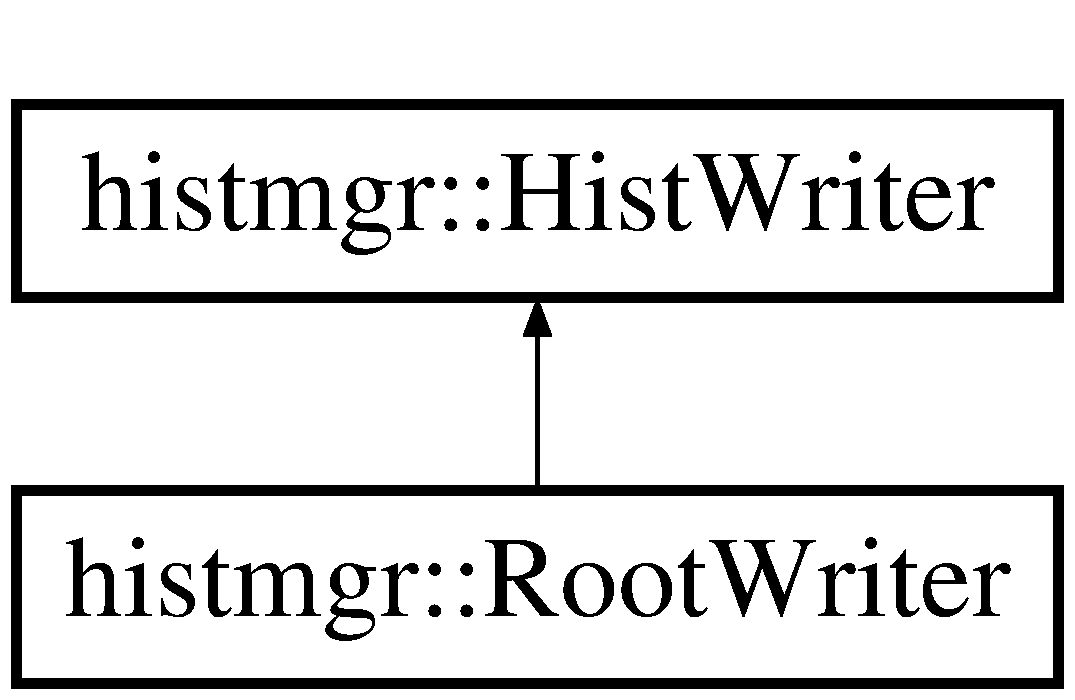
\includegraphics[height=2cm]{classhistmgr_1_1HistWriter}
\end{center}
\end{figure}
\subsection*{Public Member Functions}
\begin{DoxyCompactItemize}
\item 
virtual bool {\bf enterDir} (const std::string \&name, Bool\_\-t create=false)=0
\begin{DoxyCompactList}\small\item\em Enter a subdirectory in the file. \item\end{DoxyCompactList}\item 
virtual void {\bf upDir} ()=0\label{classhistmgr_1_1HistWriter_af4a84b802e1617ac850eb828f5d6a644}

\begin{DoxyCompactList}\small\item\em Go up one directory level. \item\end{DoxyCompactList}\item 
virtual void {\bf writeToCurrentDir} (const {\bf FloatHistogram1D} \&hist, const std::string \&name)=0
\begin{DoxyCompactList}\small\item\em Write the given histogram to a ROOT file. \item\end{DoxyCompactList}\item 
virtual void {\bf writeToCurrentDir} (const {\bf FloatHistogram2D} \&hist, const std::string \&name)=0
\begin{DoxyCompactList}\small\item\em Write the given histogram to a ROOT file. \item\end{DoxyCompactList}\item 
virtual void {\bfseries writeToCurrentDir} (const EVENT::LCGenericObject $\ast$array\_\-x, const EVENT::LCGenericObject $\ast$array\_\-y, const EVENT::LCGenericObject $\ast$array\_\-ey, const std::string \&name)=0\label{classhistmgr_1_1HistWriter_a3d8cb01d364fb517626b4b5bb990b9d1}

\end{DoxyCompactItemize}


\subsection{Detailed Description}
Abstract interface of a class to write histograms to disk. \begin{DoxySeeAlso}{See also}
\doxyref{RootWriter}{p.}{classhistmgr_1_1RootWriter}. 
\end{DoxySeeAlso}


Definition at line 16 of file HistWriter.hh.

\subsection{Member Function Documentation}
\index{histmgr::HistWriter@{histmgr::HistWriter}!enterDir@{enterDir}}
\index{enterDir@{enterDir}!histmgr::HistWriter@{histmgr::HistWriter}}
\subsubsection[{enterDir}]{\setlength{\rightskip}{0pt plus 5cm}virtual bool histmgr::HistWriter::enterDir (const std::string \& {\em name}, \/  Bool\_\-t {\em create} = {\ttfamily false})\hspace{0.3cm}{\ttfamily  [pure virtual]}}\label{classhistmgr_1_1HistWriter_adbdbc5948a21d31ee3ab9ff2e3ba1999}


Enter a subdirectory in the file. 
\begin{DoxyParams}{Parameters}
\item[{\em name}]the name of the sub directory \item[{\em create}]set to true if non existing directories shall be created \end{DoxyParams}
\begin{DoxyReturn}{Returns}
true incase the directory exists 
\end{DoxyReturn}
\index{histmgr::HistWriter@{histmgr::HistWriter}!writeToCurrentDir@{writeToCurrentDir}}
\index{writeToCurrentDir@{writeToCurrentDir}!histmgr::HistWriter@{histmgr::HistWriter}}
\subsubsection[{writeToCurrentDir}]{\setlength{\rightskip}{0pt plus 5cm}virtual void histmgr::HistWriter::writeToCurrentDir (const {\bf FloatHistogram2D} \& {\em hist}, \/  const std::string \& {\em name})\hspace{0.3cm}{\ttfamily  [pure virtual]}}\label{classhistmgr_1_1HistWriter_a3c4e7228abcd2fe54ec6748aae6407c2}


Write the given histogram to a ROOT file. 
\begin{DoxyParams}{Parameters}
\item[{\em hist}]reference to the histogram \item[{\em name}]the name given to the histogram \end{DoxyParams}


Implemented in {\bf histmgr::RootWriter} \doxyref{}{p.}{classhistmgr_1_1RootWriter_a6031ddaa5a402ae73f624fb3ea2e5970}.\index{histmgr::HistWriter@{histmgr::HistWriter}!writeToCurrentDir@{writeToCurrentDir}}
\index{writeToCurrentDir@{writeToCurrentDir}!histmgr::HistWriter@{histmgr::HistWriter}}
\subsubsection[{writeToCurrentDir}]{\setlength{\rightskip}{0pt plus 5cm}virtual void histmgr::HistWriter::writeToCurrentDir (const {\bf FloatHistogram1D} \& {\em hist}, \/  const std::string \& {\em name})\hspace{0.3cm}{\ttfamily  [pure virtual]}}\label{classhistmgr_1_1HistWriter_ad9bdd8f2a07d67c39bb0e09e79009aa5}


Write the given histogram to a ROOT file. 
\begin{DoxyParams}{Parameters}
\item[{\em hist}]reference to the histogram \item[{\em name}]the name given to the histogram \end{DoxyParams}


Implemented in {\bf histmgr::RootWriter} \doxyref{}{p.}{classhistmgr_1_1RootWriter_a14f07347e735118a227788b8a4c5a172}.

The documentation for this class was generated from the following file:\begin{DoxyCompactItemize}
\item 
HistWriter.hh\end{DoxyCompactItemize}

\section{histmgr::HistWriterKit Class Reference}
\label{classhistmgr_1_1HistWriterKit}\index{histmgr::HistWriterKit@{histmgr::HistWriterKit}}


Abstract interface of a histogram writer kit.  


{\ttfamily \#include $<$HistWriterKit.hh$>$}Inheritance diagram for histmgr::HistWriterKit::\begin{figure}[H]
\begin{center}
\leavevmode
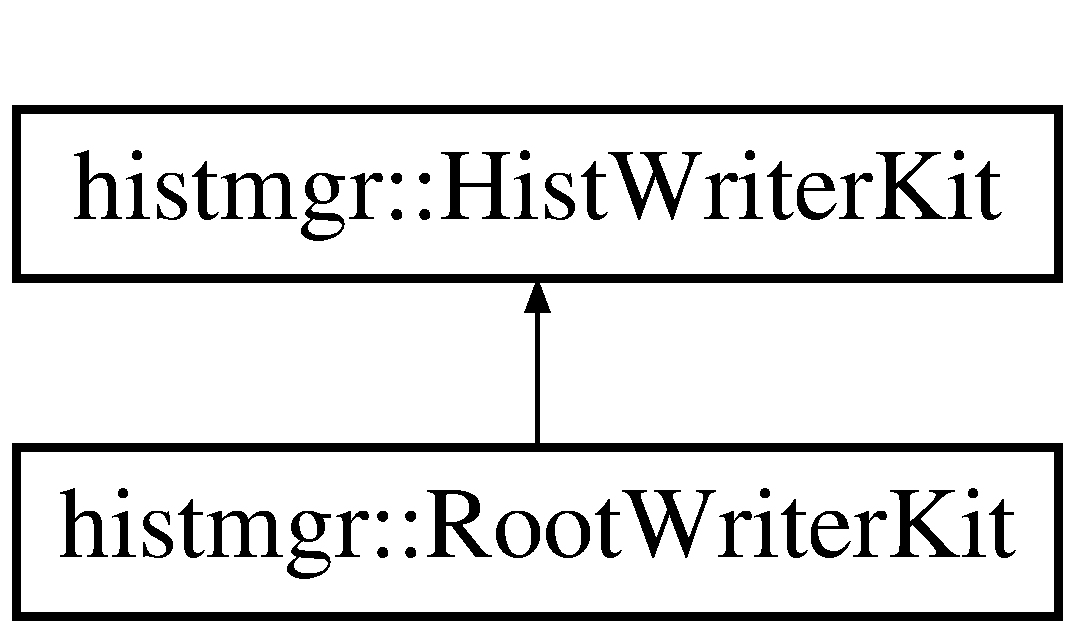
\includegraphics[height=2cm]{classhistmgr_1_1HistWriterKit}
\end{center}
\end{figure}
\subsection*{Public Member Functions}
\begin{DoxyCompactItemize}
\item 
virtual {\bf $\sim$HistWriterKit} ()
\begin{DoxyCompactList}\small\item\em Destructor. \item\end{DoxyCompactList}\item 
virtual {\bf HistWriter} $\ast$ {\bf createWriter} (const std::string \&name)=0
\begin{DoxyCompactList}\small\item\em create a histogram write. \item\end{DoxyCompactList}\end{DoxyCompactItemize}


\subsection{Detailed Description}
Abstract interface of a histogram writer kit. The writer kit is used to create the actual histogram writer. \begin{DoxySeeAlso}{See also}
\doxyref{RootWriterKit}{p.}{classhistmgr_1_1RootWriterKit} 
\end{DoxySeeAlso}


Definition at line 13 of file HistWriterKit.hh.

\subsection{Constructor \& Destructor Documentation}
\index{histmgr::HistWriterKit@{histmgr::HistWriterKit}!$\sim$HistWriterKit@{$\sim$HistWriterKit}}
\index{$\sim$HistWriterKit@{$\sim$HistWriterKit}!histmgr::HistWriterKit@{histmgr::HistWriterKit}}
\subsubsection[{$\sim$HistWriterKit}]{\setlength{\rightskip}{0pt plus 5cm}virtual histmgr::HistWriterKit::$\sim$HistWriterKit ()\hspace{0.3cm}{\ttfamily  [inline, virtual]}}\label{classhistmgr_1_1HistWriterKit_aa3c62231adb0f1f95295d27e559009a3}


Destructor. Abstract classes need a virtual destructor. 

Definition at line 19 of file HistWriterKit.hh.

\subsection{Member Function Documentation}
\index{histmgr::HistWriterKit@{histmgr::HistWriterKit}!createWriter@{createWriter}}
\index{createWriter@{createWriter}!histmgr::HistWriterKit@{histmgr::HistWriterKit}}
\subsubsection[{createWriter}]{\setlength{\rightskip}{0pt plus 5cm}virtual {\bf HistWriter}$\ast$ histmgr::HistWriterKit::createWriter (const std::string \& {\em name})\hspace{0.3cm}{\ttfamily  [pure virtual]}}\label{classhistmgr_1_1HistWriterKit_a4e07d5baf676d4af138d09f2e92b4001}


create a histogram write. 
\begin{DoxyParams}{Parameters}
\item[{\em name}]the name of the file to which the histograms should be written \end{DoxyParams}
\begin{DoxyReturn}{Returns}
a pointer a histogram writer which should be ready to write histograms. 
\end{DoxyReturn}


Implemented in {\bf histmgr::RootWriterKit} \doxyref{}{p.}{classhistmgr_1_1RootWriterKit_a480fb8728c4592098a59344922a58c71}.

The documentation for this class was generated from the following file:\begin{DoxyCompactItemize}
\item 
HistWriterKit.hh\end{DoxyCompactItemize}

\section{CALICE::HoldScanAnalysis Class Reference}
\label{classCALICE_1_1HoldScanAnalysis}\index{CALICE::HoldScanAnalysis@{CALICE::HoldScanAnalysis}}


Create Signal histograms per pad of all hits of all reconstructed clusters.  


{\ttfamily \#include $<$HoldScanAnalysis.hh$>$}Inheritance diagram for CALICE::HoldScanAnalysis::\begin{figure}[H]
\begin{center}
\leavevmode
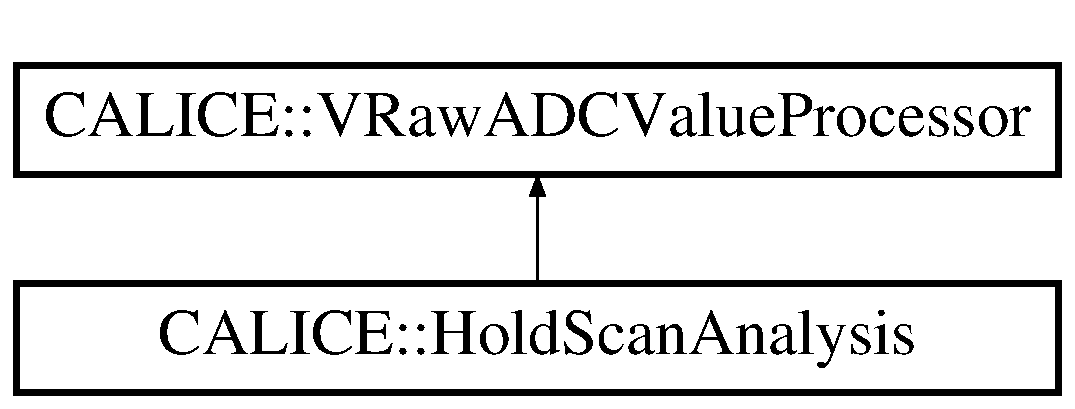
\includegraphics[height=2cm]{classCALICE_1_1HoldScanAnalysis}
\end{center}
\end{figure}
\subsection*{Public Member Functions}
\begin{DoxyCompactItemize}
\item 
Processor $\ast$ {\bfseries newProcessor} ()\label{classCALICE_1_1HoldScanAnalysis_ad5990596dee1b8767277be9526521161}

\item 
void {\bf init} ()
\begin{DoxyCompactList}\small\item\em Called at the begin of the job before anything is read. \item\end{DoxyCompactList}\item 
void {\bf processRunHeader} (LCRunHeader $\ast$run)
\begin{DoxyCompactList}\small\item\em Called for every run, e.g. \item\end{DoxyCompactList}\item 
void {\bf processEvent} (LCEvent $\ast$evtP)
\begin{DoxyCompactList}\small\item\em Called for every event -\/ the working horse. \item\end{DoxyCompactList}\item 
void {\bfseries end} ()\label{classCALICE_1_1HoldScanAnalysis_a13ed162b61891ce64fb6cfff41719b18}

\end{DoxyCompactItemize}
\subsection*{Protected Types}
\begin{DoxyCompactItemize}
\item 
enum {\bfseries EHistType} \{ {\bfseries kHistSignalPerHoldValue}, 
{\bfseries kHistTotalSignalPerHoldValue}, 
{\bfseries kNHist}
 \}
\end{DoxyCompactItemize}
\subsection*{Protected Member Functions}
\begin{DoxyCompactItemize}
\item 
void {\bf createHistograms} ()
\begin{DoxyCompactList}\small\item\em create and register histogram collections. \item\end{DoxyCompactList}\item 
void {\bf feConfChanged} (EVENT::LCCollection $\ast$col)\label{classCALICE_1_1HoldScanAnalysis_a59d01b5f9111a355a98087f22edda54c}

\begin{DoxyCompactList}\small\item\em Handle changes of Fe configuration data. \item\end{DoxyCompactList}\item 
void {\bfseries moduleTypeChanged} (lcio::LCCollection $\ast$col)\label{classCALICE_1_1HoldScanAnalysis_a13f67124dfbac5a43384720d728cd79d}

\item 
void {\bfseries moduleLocationChanged} (lcio::LCCollection $\ast$col)\label{classCALICE_1_1HoldScanAnalysis_ac7853b9f5030f2cffff1763c803c6ed4}

\item 
void {\bfseries moduleConnectionChanged} (lcio::LCCollection $\ast$col)\label{classCALICE_1_1HoldScanAnalysis_a8b1ef0f8b1806f814f738179a0c94773}

\end{DoxyCompactItemize}
\subsection*{Protected Attributes}
\begin{DoxyCompactItemize}
\item 
FloatVec {\bf \_\-signalHistPar}
\begin{DoxyCompactList}\small\item\em binning of the per hold value histograms. \item\end{DoxyCompactList}\item 
std::string {\bfseries \_\-clusterColName}\label{classCALICE_1_1HoldScanAnalysis_a821525b65e2b0658befe4572ff2b5a5b}

\item 
std::string {\bfseries \_\-feConfColName}\label{classCALICE_1_1HoldScanAnalysis_a05396b051321b994175ab5c26bc36ccd}

\item 
{\bf histmgr::Key\_\-t} {\bf \_\-histGroupKey}
\begin{DoxyCompactList}\small\item\em Key for the histogram group. \item\end{DoxyCompactList}\item 
int {\bf \_\-nHistMax}\label{classCALICE_1_1HoldScanAnalysis_a9d4b44b172ef158fc0cc865ff00c8200}

\begin{DoxyCompactList}\small\item\em Maximum number of hold values for which signal histograms can be created (parameter). \item\end{DoxyCompactList}\item 
int {\bf \_\-minNumberOfHits}
\begin{DoxyCompactList}\small\item\em Minimum number of hits of accepted clusters (parameter). \item\end{DoxyCompactList}\item 
Float\_\-t {\bf \_\-minClusterSignal}
\begin{DoxyCompactList}\small\item\em Minimum signal of accepted clusters (parameter). \item\end{DoxyCompactList}\item 
ConditionsChangeDelegator$<$ {\bf HoldScanAnalysis} $>$ {\bfseries \_\-feConfChange}\label{classCALICE_1_1HoldScanAnalysis_abc178bb058507f39db6a6b9434153141}

\item 
{\bf ModuleIndexReverseLookup} {\bfseries \_\-indexLookup}\label{classCALICE_1_1HoldScanAnalysis_a19e9e6c81508e9e2a993f980448b0255}

\item 
LCCollection $\ast$ {\bfseries \_\-nHitsHistogram}\label{classCALICE_1_1HoldScanAnalysis_a62943d737949a663b3ea9583adeb56d8}

\item 
LCCollection $\ast$ {\bfseries \_\-clusterSignalHistogram}\label{classCALICE_1_1HoldScanAnalysis_accdd2109f252c0a48d601dd3f675cbf1}

\item 
LCCollection $\ast$ {\bfseries \_\-holdValueContainer}\label{classCALICE_1_1HoldScanAnalysis_aee61abfbb2658d6b4e184604e58b6dcb}

\item 
{\bf histmgr::Key\_\-t} {\bfseries \_\-histKey} [kNHist]\label{classCALICE_1_1HoldScanAnalysis_a2d3c6efe1f8a31b54998e8fc548db0e4}

\item 
UInt\_\-t {\bfseries \_\-nHist}\label{classCALICE_1_1HoldScanAnalysis_ac9cacb21c7c4e771c1f288bb68e390d2}

\item 
std::map$<$ int, UInt\_\-t $>$ {\bfseries \_\-holdStartMap}\label{classCALICE_1_1HoldScanAnalysis_a9f62a744912af880d609661590b59cb0}

\item 
std::vector$<$ UInt\_\-t $>$ {\bfseries \_\-histogramIndex}\label{classCALICE_1_1HoldScanAnalysis_a4d69205cdc09cb052ac036b530c7ae41}

\item 
UInt\_\-t {\bfseries \_\-nClusters}\label{classCALICE_1_1HoldScanAnalysis_a1a8fa6dbaaabcf4e2059a828bd6c05e1}

\item 
UInt\_\-t {\bfseries \_\-nMissingHoldChanges}\label{classCALICE_1_1HoldScanAnalysis_afea5db3b613767acb605be6f4f6a20ca}

\item 
UInt\_\-t {\bfseries \_\-moduleIndexOutOfRange}\label{classCALICE_1_1HoldScanAnalysis_ae9a8dcd16dde44f63bc083ceabd98616}

\item 
UInt\_\-t {\bfseries \_\-nBeamOrCosmicsEvents}\label{classCALICE_1_1HoldScanAnalysis_aae4c0032da689c8bd59a62dc1a9fb23e}

\item 
UInt\_\-t {\bfseries \_\-currentCommonHoldStart}\label{classCALICE_1_1HoldScanAnalysis_a9bc44aaf4bbc5147174b8e3d813df954}

\end{DoxyCompactItemize}


\subsection{Detailed Description}
Create Signal histograms per pad of all hits of all reconstructed clusters. This class derives from \doxyref{VRawADCValueProcessor}{p.}{classCALICE_1_1VRawADCValueProcessor}, since the information about the detector is needed to setup the signal histograms. 

Definition at line 25 of file HoldScanAnalysis.hh.

\subsection{Member Function Documentation}
\index{CALICE::HoldScanAnalysis@{CALICE::HoldScanAnalysis}!createHistograms@{createHistograms}}
\index{createHistograms@{createHistograms}!CALICE::HoldScanAnalysis@{CALICE::HoldScanAnalysis}}
\subsubsection[{createHistograms}]{\setlength{\rightskip}{0pt plus 5cm}void CALICE::HoldScanAnalysis::createHistograms ()\hspace{0.3cm}{\ttfamily  [protected]}}\label{classCALICE_1_1HoldScanAnalysis_af9b442f35ad6b560ecf6736fdaa39314}


create and register histogram collections. 

Definition at line 105 of file HoldScanAnalysis.cc.

References \_\-histGroupKey, \_\-nHistMax, \_\-signalHistPar, histmgr::HistMgr::createHistogramGroup(), and histmgr::HistMgr::createHistograms().

Referenced by init().\index{CALICE::HoldScanAnalysis@{CALICE::HoldScanAnalysis}!init@{init}}
\index{init@{init}!CALICE::HoldScanAnalysis@{CALICE::HoldScanAnalysis}}
\subsubsection[{init}]{\setlength{\rightskip}{0pt plus 5cm}void CALICE::HoldScanAnalysis::init ()}\label{classCALICE_1_1HoldScanAnalysis_aa879bdea19cfbf5e5533174dc7a24c0f}


Called at the begin of the job before anything is read. Use to initialize the processor, e.g. book histograms. 

Reimplemented from {\bf CALICE::VRawADCValueProcessor} \doxyref{}{p.}{classCALICE_1_1VRawADCValueProcessor}.

Definition at line 128 of file HoldScanAnalysis.cc.

References \_\-histGroupKey, \_\-nHistMax, histmgr::HistMgr::createHistograms(), and createHistograms().\index{CALICE::HoldScanAnalysis@{CALICE::HoldScanAnalysis}!processEvent@{processEvent}}
\index{processEvent@{processEvent}!CALICE::HoldScanAnalysis@{CALICE::HoldScanAnalysis}}
\subsubsection[{processEvent}]{\setlength{\rightskip}{0pt plus 5cm}void CALICE::HoldScanAnalysis::processEvent (LCEvent $\ast$ {\em evtP})}\label{classCALICE_1_1HoldScanAnalysis_ae6c771d770ca5b456f82efe1e8c19d13}


Called for every event -\/ the working horse. 

Definition at line 161 of file HoldScanAnalysis.cc.

References \_\-histGroupKey, \_\-minClusterSignal, histmgr::HistMgr::getHistogramCollection(), CALICE::ModuleIndexReverseLookup::getModuleAndCellIndex(), and histmgr::HistogramCollection\_\-t::histogram().\index{CALICE::HoldScanAnalysis@{CALICE::HoldScanAnalysis}!processRunHeader@{processRunHeader}}
\index{processRunHeader@{processRunHeader}!CALICE::HoldScanAnalysis@{CALICE::HoldScanAnalysis}}
\subsubsection[{processRunHeader}]{\setlength{\rightskip}{0pt plus 5cm}void CALICE::HoldScanAnalysis::processRunHeader (LCRunHeader $\ast$ {\em run})\hspace{0.3cm}{\ttfamily  [inline]}}\label{classCALICE_1_1HoldScanAnalysis_ae23825d881a551a473319f0dc518bd20}


Called for every run, e.g. overwrite to initialize run dependent histograms. 

Definition at line 43 of file HoldScanAnalysis.hh.

\subsection{Field Documentation}
\index{CALICE::HoldScanAnalysis@{CALICE::HoldScanAnalysis}!\_\-histGroupKey@{\_\-histGroupKey}}
\index{\_\-histGroupKey@{\_\-histGroupKey}!CALICE::HoldScanAnalysis@{CALICE::HoldScanAnalysis}}
\subsubsection[{\_\-histGroupKey}]{\setlength{\rightskip}{0pt plus 5cm}{\bf histmgr::Key\_\-t} {\bf CALICE::HoldScanAnalysis::\_\-histGroupKey}\hspace{0.3cm}{\ttfamily  [protected]}}\label{classCALICE_1_1HoldScanAnalysis_a85e98fffce43215e0edabf5afc2b346b}


Key for the histogram group. 

Definition at line 63 of file HoldScanAnalysis.hh.

Referenced by createHistograms(), init(), and processEvent().\index{CALICE::HoldScanAnalysis@{CALICE::HoldScanAnalysis}!\_\-minClusterSignal@{\_\-minClusterSignal}}
\index{\_\-minClusterSignal@{\_\-minClusterSignal}!CALICE::HoldScanAnalysis@{CALICE::HoldScanAnalysis}}
\subsubsection[{\_\-minClusterSignal}]{\setlength{\rightskip}{0pt plus 5cm}Float\_\-t {\bf CALICE::HoldScanAnalysis::\_\-minClusterSignal}\hspace{0.3cm}{\ttfamily  [protected]}}\label{classCALICE_1_1HoldScanAnalysis_aaa4aecb1608fddf7a791e6a00e8d9aac}


Minimum signal of accepted clusters (parameter). 

Definition at line 68 of file HoldScanAnalysis.hh.

Referenced by processEvent().\index{CALICE::HoldScanAnalysis@{CALICE::HoldScanAnalysis}!\_\-minNumberOfHits@{\_\-minNumberOfHits}}
\index{\_\-minNumberOfHits@{\_\-minNumberOfHits}!CALICE::HoldScanAnalysis@{CALICE::HoldScanAnalysis}}
\subsubsection[{\_\-minNumberOfHits}]{\setlength{\rightskip}{0pt plus 5cm}int {\bf CALICE::HoldScanAnalysis::\_\-minNumberOfHits}\hspace{0.3cm}{\ttfamily  [protected]}}\label{classCALICE_1_1HoldScanAnalysis_aa13f8c6d7a4c85a4a7eb70c1ec9a02a0}


Minimum number of hits of accepted clusters (parameter). 

Definition at line 67 of file HoldScanAnalysis.hh.\index{CALICE::HoldScanAnalysis@{CALICE::HoldScanAnalysis}!\_\-signalHistPar@{\_\-signalHistPar}}
\index{\_\-signalHistPar@{\_\-signalHistPar}!CALICE::HoldScanAnalysis@{CALICE::HoldScanAnalysis}}
\subsubsection[{\_\-signalHistPar}]{\setlength{\rightskip}{0pt plus 5cm}FloatVec {\bf CALICE::HoldScanAnalysis::\_\-signalHistPar}\hspace{0.3cm}{\ttfamily  [protected]}}\label{classCALICE_1_1HoldScanAnalysis_af5d6fa8f5fce15286a9fbb3390f35391}


binning of the per hold value histograms. 

Definition at line 56 of file HoldScanAnalysis.hh.

Referenced by createHistograms().

The documentation for this class was generated from the following files:\begin{DoxyCompactItemize}
\item 
HoldScanAnalysis.hh\item 
HoldScanAnalysis.cc\end{DoxyCompactItemize}

\section{CALICE::IntegratedHcalCalibrationProcessor Class Reference}
\label{classCALICE_1_1IntegratedHcalCalibrationProcessor}\index{CALICE::IntegratedHcalCalibrationProcessor@{CALICE::IntegratedHcalCalibrationProcessor}}


The Ahcal calibration processor.  


{\ttfamily \#include $<$IntegratedHcalCalibrationProcessor.hh$>$}Inheritance diagram for CALICE::IntegratedHcalCalibrationProcessor::\begin{figure}[H]
\begin{center}
\leavevmode
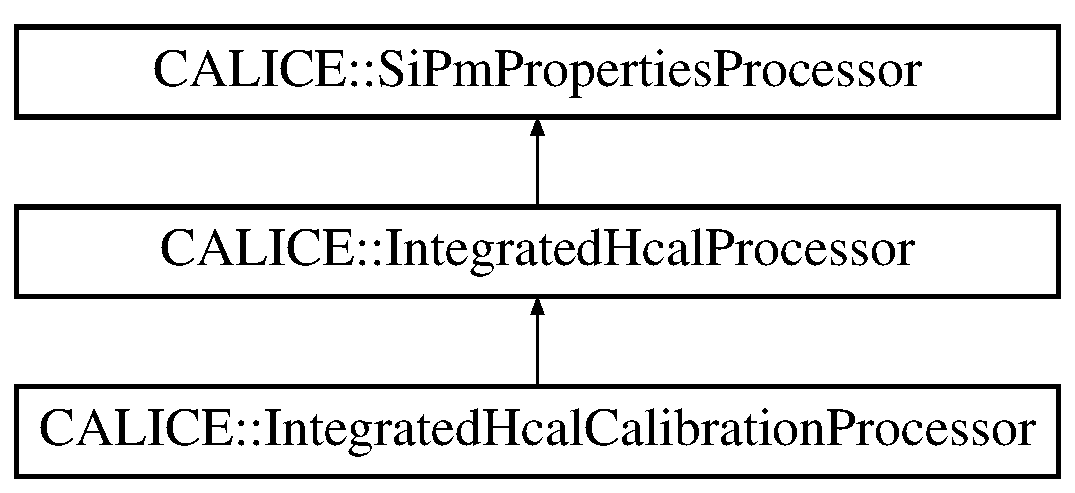
\includegraphics[height=3cm]{classCALICE_1_1IntegratedHcalCalibrationProcessor}
\end{center}
\end{figure}
\subsection*{Public Member Functions}
\begin{DoxyCompactItemize}
\item 
{\bf IntegratedHcalCalibrationProcessor} $\ast$ {\bfseries newProcessor} ()\label{classCALICE_1_1IntegratedHcalCalibrationProcessor_a598bbbd1a328ce27442d3a9d026b9867}

\item 
virtual void {\bfseries init} ()\label{classCALICE_1_1IntegratedHcalCalibrationProcessor_afcb4ac8fef8a5bcc1fd5ae4b8620af85}

\item 
virtual void {\bfseries processEvent} (lcio::LCEvent $\ast$evt)\label{classCALICE_1_1IntegratedHcalCalibrationProcessor_ae95a64ab3b6bbbd9b239f41f7d6c98c3}

\item 
virtual void {\bfseries end} ()\label{classCALICE_1_1IntegratedHcalCalibrationProcessor_a8f73d365b94979a80808dc903cfc9c00}

\end{DoxyCompactItemize}
\subsection*{Protected Attributes}
\begin{DoxyCompactItemize}
\item 
std::string {\bfseries \_\-inputColName}\label{classCALICE_1_1IntegratedHcalCalibrationProcessor_ad9b166089f6501b37a89d13c0a25bb2e}

\item 
std::string {\bfseries \_\-outputColName}\label{classCALICE_1_1IntegratedHcalCalibrationProcessor_a7b272632e6fd4e847dbb9dee88b7ceb8}

\item 
int {\bfseries \_\-zeroSuppression}\label{classCALICE_1_1IntegratedHcalCalibrationProcessor_a50776188b69d33bec8a734fcc082b22b}

\item 
float {\bfseries \_\-significanceCut}\label{classCALICE_1_1IntegratedHcalCalibrationProcessor_a0f9dbdb9a4ebc2b7955679cc64e19636}

\item 
int {\bfseries \_\-skipPedestals}\label{classCALICE_1_1IntegratedHcalCalibrationProcessor_a55d12f2aaaab3f29212109bfde96b759}

\item 
int {\bfseries \_\-minPedNumber}\label{classCALICE_1_1IntegratedHcalCalibrationProcessor_a2d709e61047bcb4cfbad62fde9d140df}

\item 
int {\bfseries \_\-pedCounter}\label{classCALICE_1_1IntegratedHcalCalibrationProcessor_ae916fee0673eb80e5acc3fdb73adc24a}

\item 
int {\bfseries \_\-pedestalSubtraction}\label{classCALICE_1_1IntegratedHcalCalibrationProcessor_a1c0d957bc70006c6f071d53799da2c5f}

\item 
float {\bfseries \_\-mipCut}\label{classCALICE_1_1IntegratedHcalCalibrationProcessor_a5670d938f278f3d4d66fbf481f0ec4c4}

\item 
bool {\bfseries \_\-doSaturationCorrection}\label{classCALICE_1_1IntegratedHcalCalibrationProcessor_aa022999f9178f6b1a8ea7575362fe8d1}

\item 
unsigned long {\bfseries \_\-hitCounter}\label{classCALICE_1_1IntegratedHcalCalibrationProcessor_a68d73faf87415a4af9a6e3a0f35476e8}

\item 
unsigned long {\bfseries \_\-invalidMIPCounter}\label{classCALICE_1_1IntegratedHcalCalibrationProcessor_a8abdbee26c81f4aa9336ff5b07ef9cde}

\item 
unsigned long {\bfseries \_\-invalidSaturationCorrectionCounter}\label{classCALICE_1_1IntegratedHcalCalibrationProcessor_a34510ab0a63023762ef2eb82b3e57587}

\item 
unsigned long {\bfseries \_\-saturationCounter}\label{classCALICE_1_1IntegratedHcalCalibrationProcessor_aaf95bbbe9b7d96f34c900eaedc800a15}

\item 
unsigned long {\bfseries \_\-eventCounter}\label{classCALICE_1_1IntegratedHcalCalibrationProcessor_a244b0feb4e3c0dbc80cdb881d33531a0}

\item 
std::map$<$ unsigned, unsigned $>$ {\bfseries \_\-invalidMIPCalibrations}\label{classCALICE_1_1IntegratedHcalCalibrationProcessor_a865d6e28f28638bf3af375cb31555db4}

\item 
std::map$<$ unsigned, unsigned $>$ {\bfseries \_\-invalidSaturationCorrections}\label{classCALICE_1_1IntegratedHcalCalibrationProcessor_a1a8724c11472e790d565b76438f3d6cc}

\item 
std::map$<$ unsigned, unsigned $>$ {\bfseries \_\-saturations}\label{classCALICE_1_1IntegratedHcalCalibrationProcessor_aec10a6498f7f035f9909bfc1d87aeeb7}

\item 
double {\bfseries \_\-pedSum} [HCAL\_\-N\_\-MOD+1][HCAL\_\-N\_\-CELL]\label{classCALICE_1_1IntegratedHcalCalibrationProcessor_a62f50a5f4d2f7b8f1a346c01f6b0d8df}

\item 
double {\bfseries \_\-pedSumSquare} [HCAL\_\-N\_\-MOD+1][HCAL\_\-N\_\-CELL]\label{classCALICE_1_1IntegratedHcalCalibrationProcessor_a452abcc49cbfe1c24f9671d1864c39a8}

\item 
unsigned {\bfseries \_\-pedNum} [HCAL\_\-N\_\-MOD+1][HCAL\_\-N\_\-CELL]\label{classCALICE_1_1IntegratedHcalCalibrationProcessor_aadb43e8133ddf7a6fc74f6812fa65d53}

\item 
float {\bfseries \_\-ped} [HCAL\_\-N\_\-MOD+1][HCAL\_\-N\_\-CELL]\label{classCALICE_1_1IntegratedHcalCalibrationProcessor_a15da76dd2514ace90b34ec890ee49f3a}

\item 
float {\bfseries \_\-pedWidth} [HCAL\_\-N\_\-MOD+1][HCAL\_\-N\_\-CELL]\label{classCALICE_1_1IntegratedHcalCalibrationProcessor_aaf5121c45f2bd9af321b74d6247186fa}

\item 
float {\bfseries \_\-pedError} [HCAL\_\-N\_\-MOD+1][HCAL\_\-N\_\-CELL]\label{classCALICE_1_1IntegratedHcalCalibrationProcessor_aa0fd128f60f5a4b034660f0ed4c5428c}

\end{DoxyCompactItemize}


\subsection{Detailed Description}
The Ahcal calibration processor. \begin{DoxyAuthor}{Author}
Sebastian Schmidt 
\end{DoxyAuthor}


Definition at line 42 of file IntegratedHcalCalibrationProcessor.hh.

The documentation for this class was generated from the following files:\begin{DoxyCompactItemize}
\item 
IntegratedHcalCalibrationProcessor.hh\item 
IntegratedHcalCalibrationProcessor.cc\end{DoxyCompactItemize}

\section{CALICE::IntegratedHcalProcessor Class Reference}
\label{classCALICE_1_1IntegratedHcalProcessor}\index{CALICE::IntegratedHcalProcessor@{CALICE::IntegratedHcalProcessor}}


Base class for all processors which need a lot of AHcal specific data, like the \doxyref{CALICE::IntegratedHcalCalibrationProcessor}{p.}{classCALICE_1_1IntegratedHcalCalibrationProcessor} and the CALICE::IntegratedHcalDigitizationProcessor.  


{\ttfamily \#include $<$IntegratedHcalProcessor.hh$>$}Inheritance diagram for CALICE::IntegratedHcalProcessor::\begin{figure}[H]
\begin{center}
\leavevmode
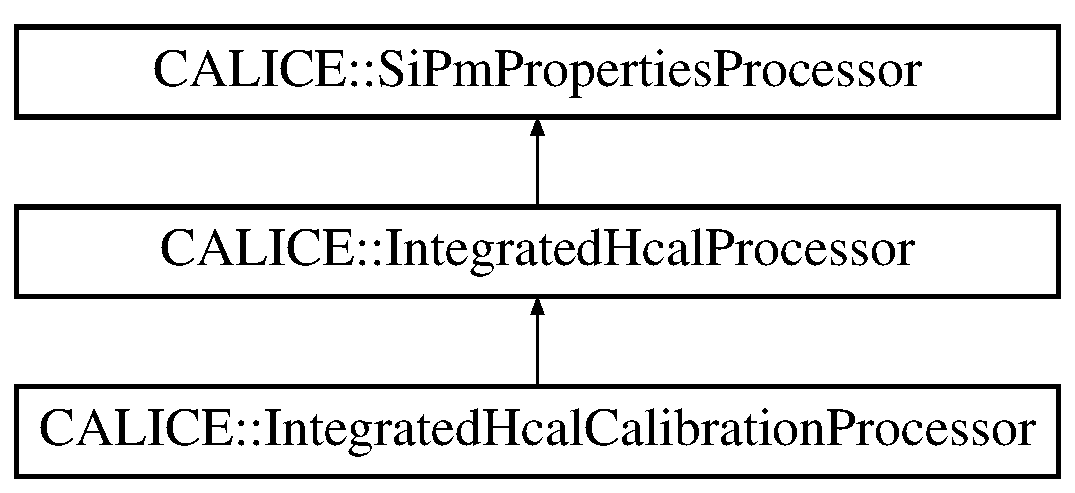
\includegraphics[height=3cm]{classCALICE_1_1IntegratedHcalProcessor}
\end{center}
\end{figure}
\subsection*{Data Structures}
\begin{DoxyCompactItemize}
\item 
struct {\bf NeighbourItem}
\begin{DoxyCompactList}\small\item\em int \_\-fudgeNonExistingSaturationCorrections; \item\end{DoxyCompactList}\end{DoxyCompactItemize}
\subsection*{Public Member Functions}
\begin{DoxyCompactItemize}
\item 
{\bf IntegratedHcalProcessor} (const std::string processorName=\char`\"{}IntegratedHcalProcessor\char`\"{})
\begin{DoxyCompactList}\small\item\em \_\-gainFitResultsMap(\&CALICE::LinearFitResult::getID), \_\-MipFitResultsMap(\&CALICE::LinearFitResult::getID), \item\end{DoxyCompactList}\item 
virtual {\bf $\sim$IntegratedHcalProcessor} ()
\item 
{\bf IntegratedHcalProcessor} $\ast$ {\bfseries newProcessor} ()\label{classCALICE_1_1IntegratedHcalProcessor_a1756ad865a23dee3410dcca7e3ea6594}

\item 
virtual void {\bf init} ()
\end{DoxyCompactItemize}
\subsection*{Protected Types}
\begin{DoxyCompactItemize}
\item 
typedef std::map$<$ unsigned, std::vector$<$ {\bf NeighbourItem} $>$ $\ast$ $>$ {\bfseries NeighbourMap}\label{classCALICE_1_1IntegratedHcalProcessor_a0bfd2769021f0a1a69ab275249d8bb81}

\end{DoxyCompactItemize}
\subsection*{Protected Member Functions}
\begin{DoxyCompactItemize}
\item 
void {\bf fillTempCountMaps} (int cellID)\label{classCALICE_1_1IntegratedHcalProcessor_af53541acd9828c24c24a915b92eb073e}

\begin{DoxyCompactList}\small\item\em Is used to fill temperature correction statistic maps. \item\end{DoxyCompactList}\item 
void {\bfseries fillTempCountMaps} (unsigned module, unsigned chip, unsigned channel)\label{classCALICE_1_1IntegratedHcalProcessor_a1f7f99d2acf5eb86bb88a66f014caf42}

\item 
void {\bf printTempCountMaps} (std::ostream \&out)\label{classCALICE_1_1IntegratedHcalProcessor_aeb33252fcb974978f913ed4e14e65d24}

\begin{DoxyCompactList}\small\item\em Is used to print temperature correction statistic maps. \item\end{DoxyCompactList}\item 
virtual void {\bf ahcSroModDataColChanged} (lcio::LCCollection $\ast$col)
\begin{DoxyCompactList}\small\item\em void IntegratedHcalProcessor::gainCalibrationChanged(lcio::LCCollection$\ast$ col) \{ ifdef HCALRECO\_\-DEBUG \item\end{DoxyCompactList}\item 
virtual void {\bfseries temperatureSensorCalibrationChanged} (lcio::LCCollection $\ast$col)\label{classCALICE_1_1IntegratedHcalProcessor_a789b552c5a5d2b9f98d23d0c0cfb78be}

\item 
virtual void {\bfseries SipmInfoChanged} (lcio::LCCollection $\ast$col)\label{classCALICE_1_1IntegratedHcalProcessor_a7f9eff7025074d0a5a573f62ecdaa198}

\item 
virtual void {\bfseries SipmSaturationChanged} (lcio::LCCollection $\ast$col)\label{classCALICE_1_1IntegratedHcalProcessor_ab191e86a502f637fc0956f5281a6fae6}

\item 
virtual void {\bfseries ModuleProductionChanged} (lcio::LCCollection $\ast$col)\label{classCALICE_1_1IntegratedHcalProcessor_a762308d52579972a065c7af24afafdb4}

\item 
virtual void {\bfseries moduleTypeChanged} (lcio::LCCollection $\ast$col)\label{classCALICE_1_1IntegratedHcalProcessor_ad82209008f52da453135a2df963e6f98}

\item 
virtual void {\bfseries moduleLocationChanged} (lcio::LCCollection $\ast$col)\label{classCALICE_1_1IntegratedHcalProcessor_ac66500e314f73a864dbddbb78a332ef0}

\item 
virtual void {\bfseries moduleConnectionChanged} (lcio::LCCollection $\ast$col)\label{classCALICE_1_1IntegratedHcalProcessor_a0062408fe85891e299dc2dfd6702c5c5}

\item 
float {\bf getMip} (int CellID)
\begin{DoxyCompactList}\small\item\em Use this function to get the Mip constant of a cell. \item\end{DoxyCompactList}\item 
float {\bf getCorrectedAmplitude} (int cellID, float satAmpl)\label{classCALICE_1_1IntegratedHcalProcessor_a88d95564a2e46cf8859f37ac20f18cad}

\begin{DoxyCompactList}\small\item\em float getMip(unsigned int module, unsigned int chip, unsigned int channel); \item\end{DoxyCompactList}\item 
float {\bfseries getSaturatedAmplitude} (int cellID, float linAmpl)\label{classCALICE_1_1IntegratedHcalProcessor_afa0e0dd7c1dbd94bf9c424e1ad45a6ea}

\item 
float {\bf getGain} (int cellID)
\begin{DoxyCompactList}\small\item\em Use this function to get the Gain constant of a cell. \item\end{DoxyCompactList}\item 
float {\bf getIC} (int cellID)
\begin{DoxyCompactList}\small\item\em float getGain(unsigned int module, unsigned int chip, unsigned int channel); \item\end{DoxyCompactList}\item 
float {\bf getCellTemp} (int cellID)\label{classCALICE_1_1IntegratedHcalProcessor_a417b653d6ab575ded3a10ff860f18a85}

\begin{DoxyCompactList}\small\item\em float getIC(unsigned int module, unsigned int chip, unsigned int channel); \item\end{DoxyCompactList}\item 
float {\bfseries getCellTemp} (unsigned int module, unsigned int chip, unsigned int channel)\label{classCALICE_1_1IntegratedHcalProcessor_adb26bbccc99eafa88a192c0c70282e6f}

\item 
std::pair$<$ unsigned int, unsigned int $>$ {\bfseries getModuleIDandCellkey} (unsigned int module, unsigned int chip, unsigned int channel)\label{classCALICE_1_1IntegratedHcalProcessor_aeebb764248fff7bc69b29d6db13204da}

\item 
void {\bfseries updateGeometryMaps} ()\label{classCALICE_1_1IntegratedHcalProcessor_ae4ce3d127835924c41361acbebc3be28}

\item 
std::vector$<$ {\bf NeighbourItem} $>$ $\ast$ {\bfseries getNeighbourList} (const unsigned short module, const unsigned cellkey) const \label{classCALICE_1_1IntegratedHcalProcessor_a4ae51b0fc8bf833f00e1563382875b33}

\item 
int {\bfseries reverseLookup} (int I, int J, int K) const \label{classCALICE_1_1IntegratedHcalProcessor_a91f4d1c50a77782f37e8cf1f14ac82f5}

\item 
int {\bfseries geometricalLookup} (int module, int chip, int channel)\label{classCALICE_1_1IntegratedHcalProcessor_a17ede3cc89f52980a83e2e0abe362a75}

\end{DoxyCompactItemize}
\subsection*{Protected Attributes}
\begin{DoxyCompactItemize}
\item 
bool {\bfseries \_\-doMipTempCorr}\label{classCALICE_1_1IntegratedHcalProcessor_a2b3b326d43f7dcf0d988baaa016bfa58}

\item 
bool {\bfseries \_\-doGainTempCorr}\label{classCALICE_1_1IntegratedHcalProcessor_a91b9fe707133bb82554271e48e55fe02}

\item 
std::map$<$ unsigned, unsigned $>$ {\bf \_\-cellOccurenceCounter}
\begin{DoxyCompactList}\small\item\em Use this map to count how often the cell specified with the HcalTileIndex occurs during calibration or digitization in the whole run. \item\end{DoxyCompactList}\item 
std::map$<$ unsigned, unsigned $>$ {\bf \_\-cellMipTempCorrCounter}
\begin{DoxyCompactList}\small\item\em Use this map to count how often the cell specified with the HcalTileIndex is calibrated or digitized with a temperature corrected Mip constant. \item\end{DoxyCompactList}\item 
std::map$<$ unsigned, unsigned $>$ {\bf \_\-cellNoMipTempCorrCounter}
\begin{DoxyCompactList}\small\item\em Use this map to count how often the cell specified with the HcalTileIndex is calibrated or digitized using a Mip constant without temperature correction. \item\end{DoxyCompactList}\item 
std::map$<$ unsigned, unsigned $>$ {\bf \_\-cellGainTempCorrCounter}
\begin{DoxyCompactList}\small\item\em Use this map to count how often the cell specified with the HcalTileIndex is calibrated or digitized with a temperature corrected Gain constant. \item\end{DoxyCompactList}\item 
std::map$<$ unsigned, unsigned $>$ {\bf \_\-cellNoGainTempCorrCounter}
\begin{DoxyCompactList}\small\item\em Use this map to count how often the cell specified with the HcalTileIndex is calibrated or digitized using a Gain constant without temperature correction. \item\end{DoxyCompactList}\item 
bool {\bf \_\-cellCalibUsedMipTempCorr}
\begin{DoxyCompactList}\small\item\em This flags shows whether the current cell is calibrated or digitized with a temperature corrected mip constant or not. \item\end{DoxyCompactList}\item 
bool {\bf \_\-cellCalibUsedGainTempCorr}
\begin{DoxyCompactList}\small\item\em This flags shows whether the current cell is calibrated or digitized with a temperature corrected mip constant or not. \item\end{DoxyCompactList}\item 
std::string {\bfseries \_\-gainCalColName}\label{classCALICE_1_1IntegratedHcalProcessor_a40fcfe93120bef56b0bdc790a26fc462}

\item 
std::string {\bfseries \_\-interCalColName}\label{classCALICE_1_1IntegratedHcalProcessor_ab8121fe4f449cc9b0a859ddd54dfd089}

\item 
std::string {\bfseries \_\-mipCalColName}\label{classCALICE_1_1IntegratedHcalProcessor_a16394fd12e15b65cd9c5e4e98acf64da}

\item 
std::string {\bfseries \_\-ahcSroModDataColName}\label{classCALICE_1_1IntegratedHcalProcessor_a70140ada65f48e8b681694d342ff43ef}

\item 
std::string {\bfseries \_\-colNameModuleDescription}\label{classCALICE_1_1IntegratedHcalProcessor_a62b331db047f75432bbe71f2e540346d}

\item 
std::string {\bfseries \_\-colNameModuleLocation}\label{classCALICE_1_1IntegratedHcalProcessor_a1071290475af63de89c4e157a6c9adce}

\item 
std::string {\bfseries \_\-colNameModuleConnection}\label{classCALICE_1_1IntegratedHcalProcessor_a55180d508f4ab66f8992f4cf06b9c973}

\item 
std::string {\bfseries \_\-temperatureSensorCalibrationColName}\label{classCALICE_1_1IntegratedHcalProcessor_a702fc5e8b442a72ba1dc10b05e046ae9}

\item 
AhcTempProvider $\ast$ {\bfseries \_\-tempProvider}\label{classCALICE_1_1IntegratedHcalProcessor_a5b41cba62cd72b22d8e84c553c27547c}

\item 
lccd::ConditionsMap$<$ int, CALICE::LinearFitConstant $>$ {\bfseries \_\-gainFitConstantsMap}\label{classCALICE_1_1IntegratedHcalProcessor_a16f74752283b7213211955642c24adf7}

\item 
lccd::ConditionsMap$<$ int, CALICE::LinearFitSlope $>$ {\bfseries \_\-gainFitSlopesMap}\label{classCALICE_1_1IntegratedHcalProcessor_a3ed7cb66c11825e22df586f16b008987}

\item 
lccd::ConditionsMap$<$ int, CALICE::LinearFitConstant $>$ {\bfseries \_\-MipFitConstantsMap}\label{classCALICE_1_1IntegratedHcalProcessor_a27106155fa040cc474cdb19b6d0fde26}

\item 
lccd::ConditionsMap$<$ int, CALICE::LinearFitSlope $>$ {\bfseries \_\-MipFitSlopesMap}\label{classCALICE_1_1IntegratedHcalProcessor_adfb1960abe0ed795e0ea00a502273b4b}

\item 
lccd::ConditionsMap$<$ const int, CALICE::SatCorrItep $>$ {\bfseries \_\-SatCorrMap}\label{classCALICE_1_1IntegratedHcalProcessor_a656e486cedc3eb7c1660f1eaa54a93b9}

\item 
lccd::ConditionsMap$<$ int, CALICE::LinearFitConstant $>$ {\bfseries \_\-InterConstantsMap}\label{classCALICE_1_1IntegratedHcalProcessor_a7f517e8fc14737205ba1a5d599eccad1}

\item 
std::string {\bfseries \_\-gainFitConstantsCollectionName}\label{classCALICE_1_1IntegratedHcalProcessor_a3349b45b04410e56b6127de149c2971b}

\item 
std::string {\bfseries \_\-MipFitConstantsCollectionName}\label{classCALICE_1_1IntegratedHcalProcessor_a8f5e2fe335aba5f95811cbe6e378cbf7}

\item 
std::string {\bfseries \_\-SatCorrCollectionName}\label{classCALICE_1_1IntegratedHcalProcessor_a00a60e9a07361a03ebf69ca837348aea}

\item 
std::string {\bfseries \_\-gainFitSlopesCollectionName}\label{classCALICE_1_1IntegratedHcalProcessor_a0172b42b0662f1051c293605c282274d}

\item 
std::string {\bfseries \_\-MipFitSlopesCollectionName}\label{classCALICE_1_1IntegratedHcalProcessor_a854a49311e1fcc228ac6d30779b1340a}

\item 
std::string {\bfseries \_\-InterConstantsCollectionName}\label{classCALICE_1_1IntegratedHcalProcessor_a1e6a00e7aced2c44317b0865145b927f}

\item 
IntVec {\bf \_\-modules}\label{classCALICE_1_1IntegratedHcalProcessor_a1b03f52aa888d675035ccf0c3e533994}

\begin{DoxyCompactList}\small\item\em CalibrationSet$<$GainConstants$>$$\ast$ \_\-gainCalibSet; CalibrationSet$<$InterConstants$>$$\ast$ \_\-interCalibSet; CalibrationSet$<$MIPConstants$>$$\ast$ \_\-mipCalibSet;. \item\end{DoxyCompactList}\item 
float {\bfseries \_\-gainScalingFactor}\label{classCALICE_1_1IntegratedHcalProcessor_afd0793107948e1b518bc48edf2f902c3}

\item 
float {\bfseries \_\-mipScalingFactor}\label{classCALICE_1_1IntegratedHcalProcessor_abb530fcd9b374a9b41f42b2f27e91c64}

\item 
{\bf HcalTempModel} $\ast$ {\bfseries \_\-tempModel}\label{classCALICE_1_1IntegratedHcalProcessor_add2ba4229041de00306f3265412af375}

\item 
MappingAndAlignment {\bfseries \_\-mapping}\label{classCALICE_1_1IntegratedHcalProcessor_aea7df0eff16f7759ea41789b0e3886d0}

\item 
HcalModuleIndexReverseLookup {\bfseries \_\-indexLookup}\label{classCALICE_1_1IntegratedHcalProcessor_a40bd029718e50227668cef2246783bc6}

\item 
int {\bfseries \_\-viewConnectionTree}\label{classCALICE_1_1IntegratedHcalProcessor_a4fd6516291240ccdaeecefca4bf40ad1}

\item 
std::map$<$ unsigned, unsigned $>$ {\bfseries \_\-inverseModuleMap}\label{classCALICE_1_1IntegratedHcalProcessor_a307a2681e8856810362e166080ec4795}

\item 
std::map$<$ unsigned, unsigned $>$ {\bfseries \_\-cellMap}\label{classCALICE_1_1IntegratedHcalProcessor_a99d9a6d6bd972756bd8cb8e6d1b37ea5}

\item 
NeighbourMap {\bfseries \_\-neighbourMap}\label{classCALICE_1_1IntegratedHcalProcessor_ac3c877341fc3fd71315b67abfcaa701a}

\item 
ConditionsChangeDelegator$<$ {\bf IntegratedHcalProcessor} $>$ {\bf \_\-ahcSroModDataChange}\label{classCALICE_1_1IntegratedHcalProcessor_a9b73ff8cf620b9ca23f3820413c0ff9c}

\begin{DoxyCompactList}\small\item\em ConditionsChangeDelegator$<$IntegratedHcalProcessor$>$ \_\-gainCalibrationChange; ConditionsChangeDelegator$<$IntegratedHcalProcessor$>$ \_\-interCalibrationChange; ConditionsChangeDelegator$<$IntegratedHcalProcessor$>$ \_\-mipCalibrationChange;. \item\end{DoxyCompactList}\item 
ConditionsChangeDelegator$<$ {\bf IntegratedHcalProcessor} $>$ {\bfseries \_\-temperatureSensorCalibrationChange}\label{classCALICE_1_1IntegratedHcalProcessor_a1148d25fd93f901f71f404ba01bcd026}

\item 
ConditionsChangeDelegator$<$ {\bf IntegratedHcalProcessor} $>$ {\bfseries \_\-moduleTypeChange}\label{classCALICE_1_1IntegratedHcalProcessor_a9356228a9c3859031a0b0b52e0034cab}

\item 
ConditionsChangeDelegator$<$ {\bf IntegratedHcalProcessor} $>$ {\bfseries \_\-moduleLocationChange}\label{classCALICE_1_1IntegratedHcalProcessor_a10fa4eb77c7eb393e8fe709b0b4f5d18}

\item 
ConditionsChangeDelegator$<$ {\bf IntegratedHcalProcessor} $>$ {\bfseries \_\-moduleConnectionChange}\label{classCALICE_1_1IntegratedHcalProcessor_a45e69354f1b5b49d548fb138f76aff8a}

\item 
lcio::LCCollection $\ast$ {\bfseries \_\-ahcSroModDataCol}\label{classCALICE_1_1IntegratedHcalProcessor_a533260a9dd56825f6044544918458e52}

\end{DoxyCompactItemize}
\subsection*{Private Member Functions}
\begin{DoxyCompactItemize}
\item 
void {\bfseries considerNeighbourRelation} (const unsigned centralCellIndex, const int rowOffset, const int columnOffset)\label{classCALICE_1_1IntegratedHcalProcessor_ada73b452af34c6c39b4f2972571fcb66}

\item 
void {\bfseries establishTileCoverage} (const unsigned centralCellIndex, const int rowOffset, const int columnOffset)\label{classCALICE_1_1IntegratedHcalProcessor_ac2d61eaf3e4a5083cbd9cf272c7d005d}

\end{DoxyCompactItemize}
\subsection*{Private Attributes}
\begin{DoxyCompactItemize}
\item 
int {\bfseries \_\-doSatScaling}\label{classCALICE_1_1IntegratedHcalProcessor_add82a2f652cff16a0eb8bb26b6503b38}

\end{DoxyCompactItemize}


\subsection{Detailed Description}
Base class for all processors which need a lot of AHcal specific data, like the \doxyref{CALICE::IntegratedHcalCalibrationProcessor}{p.}{classCALICE_1_1IntegratedHcalCalibrationProcessor} and the CALICE::IntegratedHcalDigitizationProcessor. \begin{DoxyAuthor}{Author}
Sebastian Schmidt 
\end{DoxyAuthor}


Definition at line 58 of file IntegratedHcalProcessor.hh.

\subsection{Constructor \& Destructor Documentation}
\index{CALICE::IntegratedHcalProcessor@{CALICE::IntegratedHcalProcessor}!IntegratedHcalProcessor@{IntegratedHcalProcessor}}
\index{IntegratedHcalProcessor@{IntegratedHcalProcessor}!CALICE::IntegratedHcalProcessor@{CALICE::IntegratedHcalProcessor}}
\subsubsection[{IntegratedHcalProcessor}]{\setlength{\rightskip}{0pt plus 5cm}CALICE::IntegratedHcalProcessor::IntegratedHcalProcessor (const std::string {\em processorName} = {\ttfamily \char`\"{}IntegratedHcalProcessor\char`\"{}})}\label{classCALICE_1_1IntegratedHcalProcessor_a1f9c46f39106dd619be790c45c3e93eb}


\_\-gainFitResultsMap(\&CALICE::LinearFitResult::getID), \_\-MipFitResultsMap(\&CALICE::LinearFitResult::getID), \_\-gainCalibrationChange(this,\&IntegratedHcalProcessor::gainCalibrationChanged), \_\-interCalibrationChange(this,\&IntegratedHcalProcessor::interCalibrationChanged), \_\-mipCalibrationChange(this,\&IntegratedHcalProcessor::mipCalibrationChanged), 

registerProcessorParameter(\char`\"{}GainCalibrationCollectionTemplate\char`\"{}, \char`\"{}Template for the name of the module wise collections with the gain calibration constants\char`\"{}, \_\-gainCalColName, std::string(\char`\"{}Gain\_\-\char`\"{}));

registerProcessorParameter(\char`\"{}InterCalibrationCollectionTemplate\char`\"{}, \char`\"{}Template for the name of the module wise collections with the inter calibration constants\char`\"{}, \_\-interCalColName, std::string(\char`\"{}IC\_\-\char`\"{}));

registerProcessorParameter(\char`\"{}MIPCalibrationCollectionTemplate\char`\"{}, \char`\"{}Template for the name of the module wise collections with the MIP calibration constants\char`\"{}, \_\-mipCalColName, std::string(\char`\"{}MIP\_\-\char`\"{}));

registerProcessorParameter(\char`\"{}FudgeNonExistingSaturationCorrections\char`\"{}, \char`\"{}set saturation corrections to 1 (1) or to 0 (0) if they don't exist\char`\"{}, \_\-fudgeNonExistingSaturationCorrections, (int) 0);

registerProcessorParameter(\char`\"{}CorrectLYSat\char`\"{},\char`\"{}\char`\"{}, \_\-correctSatLY, false);

\_\-gainCalibSet = new CalibrationSet$<$GainConstants$>$(\_\-tempModel); \_\-interCalibSet = new CalibrationSet$<$InterConstants$>$(\_\-tempModel); \_\-mipCalibSet = new CalibrationSet$<$MIPConstants$>$(\_\-tempModel); 

Definition at line 36 of file IntegratedHcalProcessor.cc.

References \_\-modules.\index{CALICE::IntegratedHcalProcessor@{CALICE::IntegratedHcalProcessor}!$\sim$IntegratedHcalProcessor@{$\sim$IntegratedHcalProcessor}}
\index{$\sim$IntegratedHcalProcessor@{$\sim$IntegratedHcalProcessor}!CALICE::IntegratedHcalProcessor@{CALICE::IntegratedHcalProcessor}}
\subsubsection[{$\sim$IntegratedHcalProcessor}]{\setlength{\rightskip}{0pt plus 5cm}CALICE::IntegratedHcalProcessor::$\sim$IntegratedHcalProcessor ()\hspace{0.3cm}{\ttfamily  [virtual]}}\label{classCALICE_1_1IntegratedHcalProcessor_aab224b9608bde19e5aafa8c3c06f73ca}


if ( \_\-gainCalibSet ) delete \_\-gainCalibSet; if ( \_\-interCalibSet ) delete \_\-interCalibSet; if ( \_\-mipCalibSet ) delete \_\-mipCalibSet; 

Definition at line 164 of file IntegratedHcalProcessor.cc.

\subsection{Member Function Documentation}
\index{CALICE::IntegratedHcalProcessor@{CALICE::IntegratedHcalProcessor}!ahcSroModDataColChanged@{ahcSroModDataColChanged}}
\index{ahcSroModDataColChanged@{ahcSroModDataColChanged}!CALICE::IntegratedHcalProcessor@{CALICE::IntegratedHcalProcessor}}
\subsubsection[{ahcSroModDataColChanged}]{\setlength{\rightskip}{0pt plus 5cm}void CALICE::IntegratedHcalProcessor::ahcSroModDataColChanged (lcio::LCCollection $\ast$ {\em col})\hspace{0.3cm}{\ttfamily  [protected, virtual]}}\label{classCALICE_1_1IntegratedHcalProcessor_af154b6a1ea4688828bb3d5fc297a6005}


void IntegratedHcalProcessor::gainCalibrationChanged(lcio::LCCollection$\ast$ col) \{ ifdef HCALRECO\_\-DEBUG std::cout $<$$<$ \char`\"{}IntegratedHcalProcessor::gainCalibrationChanged()\char`\"{} $<$$<$ std::endl; endif \_\-gainCalibSet-\/$>$setScalingFactor( \_\-gainScalingFactor ); if (\_\-ahcSroModDataCol) \_\-gainCalibSet-\/$>$fill(col, \_\-ahcSroModDataCol); else \_\-gainCalibSet-\/$>$fill(col); \_\-gainCalibSet-\/$>$applyScalingFactor( \_\-gainScalingFactor ); calculateLightYield(); \}; void IntegratedHcalProcessor::interCalibrationChanged(lcio::LCCollection$\ast$ col) \{ ifdef HCALRECO\_\-DEBUG std::cout $<$$<$ \char`\"{}IntegratedHcalProcessor::interCalibrationChanged()\char`\"{} $<$$<$ std::endl; endif if (\_\-ahcSroModDataCol) \_\-interCalibSet-\/$>$fill(col, \_\-ahcSroModDataCol); else \_\-interCalibSet-\/$>$fill(col); calculateLightYield(); \}; void IntegratedHcalProcessor::mipCalibrationChanged(lcio::LCCollection$\ast$ col) \{ ifdef HCALRECO\_\-DEBUG std::cout $<$$<$ \char`\"{}IntegratedHcalProcessor::mipCalibrationChanged()\char`\"{} $<$$<$ std::endl; endif \_\-mipCalibSet-\/$>$setScalingFactor( \_\-mipScalingFactor ); if (\_\-ahcSroModDataCol) \_\-mipCalibSet-\/$>$fill(col, \_\-ahcSroModDataCol); else \_\-mipCalibSet-\/$>$fill(col); \_\-mipCalibSet-\/$>$applyScalingFactor( \_\-mipScalingFactor ); calculateLightYield(); \}; 

\_\-gainCalibSet-\/$>$setTemp(\_\-ahcSroModDataCol); \_\-interCalibSet-\/$>$setTemp(\_\-ahcSroModDataCol); \_\-mipCalibSet-\/$>$setTemp(\_\-ahcSroModDataCol); 

Definition at line 369 of file IntegratedHcalProcessor.cc.\index{CALICE::IntegratedHcalProcessor@{CALICE::IntegratedHcalProcessor}!getGain@{getGain}}
\index{getGain@{getGain}!CALICE::IntegratedHcalProcessor@{CALICE::IntegratedHcalProcessor}}
\subsubsection[{getGain}]{\setlength{\rightskip}{0pt plus 5cm}float CALICE::IntegratedHcalProcessor::getGain (int {\em cellID})\hspace{0.3cm}{\ttfamily  [protected]}}\label{classCALICE_1_1IntegratedHcalProcessor_a99aee82ab26b548395aedb40448bf45b}


Use this function to get the Gain constant of a cell. float \doxyref{IntegratedHcalProcessor::getMip}{p.}{classCALICE_1_1IntegratedHcalProcessor_a4c9a7ff2de71086a63f297a74c0e96ca}(unsigned int module, unsigned int chip, unsigned int channel) \{ streamlog\_\-out(DEBUG0) $<$$<$ \char`\"{}-\/-\/getMip() started\char`\"{} $<$$<$ std::endl; \_\-cellCalibUsedMipTempCorr = false;

This includes temperature correction.

if( \_\-doMipTempCorr ) \{ try \{

LinearFitConstant\& MipFitConstant = \_\-MipFitConstantsMap.find(HcalTileIndex( module, chip, channel).getIndex()); const LinearFitSlope\& MipFitSlope = \_\-MipFitSlopesMap.find(HcalTileIndex( module, chip, channel).getIndex());

MipFitConstant.setSlope(MipFitSlope.getSlope());

const double currentTemperature = getCellTemp(module, chip, channel);

streamlog\_\-out(DEBUG4) $<$$<$ \char`\"{}Using mip temperature dependency\char`\"{} $<$$<$ std::endl;

\_\-cellCalibUsedMipTempCorr=true; streamlog\_\-out(DEBUG0) $<$$<$ \char`\"{}-\/-\/getMip() ended\char`\"{} $<$$<$ std::endl;

return MipFitConstant.eval(currentTemperature);

\} catch(lcio::Exception e) \{

streamlog\_\-out(DEBUG4) $<$$<$ \char`\"{}No mip temperature dependency found for \char`\"{} $<$$<$ \char`\"{}module: \char`\"{} $<$$<$ module $<$$<$ \char`\"{} chip: \char`\"{} $<$$<$ chip $<$$<$ \char`\"{} channel: \char`\"{} $<$$<$ channel $<$$<$ '\par
' $<$$<$ \char`\"{}Using fall back constant.\char`\"{} $<$$<$ std::endl; \} \}

std::pair$<$unsigned int, unsigned int$>$ IDandKey = getModuleIDandCellkey(module,chip,channel);

int moduleid = IDandKey.first; int cellkey = IDandKey.second;

MIPConstants$\ast$ mipCalib = \_\-mipCalibSet-\/$>$getCalib(moduleid, cellkey);

default mip is 100000 float mip = 100000; if ( mipCalib ) \{ mip = mipCalib-\/$>$getMIPValue(); \}

\_\-cellCalibUsedMipTempCorr = false; streamlog\_\-out(DEBUG0) $<$$<$ \char`\"{}-\/-\/getMip() ended\char`\"{} $<$$<$ std::endl; return mip;

\}; 

return 400; HcalTileIndex hti( cellID ); streamlog\_\-out(DEBUG4) $<$$<$ \char`\"{}No gain temperature dependency found for \char`\"{} $<$$<$ \char`\"{}module: \char`\"{} $<$$<$ hti.getModule() $<$$<$ \char`\"{} chip: \char`\"{} $<$$<$ hti.getChip() $<$$<$ \char`\"{} channel: \char`\"{} $<$$<$ hti.getChannel() $<$$<$ '\par
' $<$$<$ \char`\"{}Using fall back constant.\char`\"{} $<$$<$ std::endl;

return getGain( hti.getModule(), hti.getChip(), hti.getChannel() ); 

Definition at line 641 of file IntegratedHcalProcessor.cc.

References \_\-cellCalibUsedGainTempCorr, and getCellTemp().\index{CALICE::IntegratedHcalProcessor@{CALICE::IntegratedHcalProcessor}!getIC@{getIC}}
\index{getIC@{getIC}!CALICE::IntegratedHcalProcessor@{CALICE::IntegratedHcalProcessor}}
\subsubsection[{getIC}]{\setlength{\rightskip}{0pt plus 5cm}float CALICE::IntegratedHcalProcessor::getIC (int {\em cellID})\hspace{0.3cm}{\ttfamily  [protected]}}\label{classCALICE_1_1IntegratedHcalProcessor_af8083a34cd5d30ab682dde74c536bbe4}


float getGain(unsigned int module, unsigned int chip, unsigned int channel); float \doxyref{IntegratedHcalProcessor::getGain}{p.}{classCALICE_1_1IntegratedHcalProcessor_a99aee82ab26b548395aedb40448bf45b}(unsigned int module, unsigned int chip, unsigned int channel) \{ streamlog\_\-out(DEBUG0) $<$$<$ \char`\"{}-\/-\/getGain() started\char`\"{} $<$$<$ std::endl;

\_\-cellCalibUsedGainTempCorr = false;

std::pair$<$unsigned int, unsigned int$>$ IDandKey = getModuleIDandCellkey(module,chip,channel);

int moduleid = IDandKey.first; int cellkey = IDandKey.second;

GainConstants$\ast$ gainCalib = \_\-gainCalibSet-\/$>$getCalib(moduleid, cellkey);

default gain is 400 float gain = 400; if ( gainCalib ) \{ gain = gainCalib-\/$>$getGainValue(); \}

\_\-cellCalibUsedGainTempCorr = false; streamlog\_\-out(DEBUG0) $<$$<$ \char`\"{}-\/-\/getGain() ended\char`\"{} $<$$<$ std::endl; return gain;

\}; 

HcalTileIndex hti( cellID ); return getIC( hti.getModule(), hti.getChip(), hti.getChannel() ); 

Definition at line 711 of file IntegratedHcalProcessor.cc.\index{CALICE::IntegratedHcalProcessor@{CALICE::IntegratedHcalProcessor}!getMip@{getMip}}
\index{getMip@{getMip}!CALICE::IntegratedHcalProcessor@{CALICE::IntegratedHcalProcessor}}
\subsubsection[{getMip}]{\setlength{\rightskip}{0pt plus 5cm}float CALICE::IntegratedHcalProcessor::getMip (int {\em CellID})\hspace{0.3cm}{\ttfamily  [protected]}}\label{classCALICE_1_1IntegratedHcalProcessor_a4c9a7ff2de71086a63f297a74c0e96ca}


Use this function to get the Mip constant of a cell. This includes temperature correction. 

return 100000; HcalTileIndex hti( cellID ); streamlog\_\-out(DEBUG4) $<$$<$ \char`\"{}No mip temperature dependency found for \char`\"{} $<$$<$ \char`\"{}module: \char`\"{} $<$$<$ hti.getModule() $<$$<$ \char`\"{} chip: \char`\"{} $<$$<$ hti.getChip() $<$$<$ \char`\"{} channel: \char`\"{} $<$$<$ hti.getChannel() $<$$<$ '\par
' $<$$<$ \char`\"{}Using fall back constant.\char`\"{} $<$$<$ std::endl; return getMip( hti.getModule(), hti.getChip(), hti.getChannel() ); 

Definition at line 539 of file IntegratedHcalProcessor.cc.

References \_\-cellCalibUsedMipTempCorr, and getCellTemp().\index{CALICE::IntegratedHcalProcessor@{CALICE::IntegratedHcalProcessor}!init@{init}}
\index{init@{init}!CALICE::IntegratedHcalProcessor@{CALICE::IntegratedHcalProcessor}}
\subsubsection[{init}]{\setlength{\rightskip}{0pt plus 5cm}void CALICE::IntegratedHcalProcessor::init ()\hspace{0.3cm}{\ttfamily  [virtual]}}\label{classCALICE_1_1IntegratedHcalProcessor_a72760a0c4f8d4c8ec362a2d3b7e0eb4c}


if (parameterSet(\char`\"{}Module\char`\"{})) \{ unsigned index = 0 ; message $<$$<$ \char`\"{}Missing condition data: \char`\"{}; while (index $<$ \_\-modules.size() )\{

char \_\-mod[10]; sprintf(\_\-mod,\char`\"{}\%.2d\char`\"{},\_\-modules[index++]); std::string \_\-module(\_\-mod);

std::string \_\-finalGainCalColName = \_\-gainCalColName + \_\-module; if (!marlinConditionsProcessor::registerChangeListener (\&\_\-gainCalibrationChange ,\_\-finalGainCalColName)) \{ message $<$$<$ \char`\"{} \char`\"{} $<$$<$ \_\-finalGainCalColName; error=true; \} else \{ ifdef HCALRECO\_\-DEBUG std::cout $<$$<$ \char`\"{}IntegratedHcalProcessor: register conditions data handler for gain calibration collection \char`\"{} $<$$<$ \_\-finalGainCalColName $<$$<$ std::endl; endif \} std::string \_\-finalInterCalColName = \_\-interCalColName + \_\-module; if (!marlinConditionsProcessor::registerChangeListener (\&\_\-interCalibrationChange ,\_\-finalInterCalColName)) \{ message $<$$<$ \char`\"{} \char`\"{} $<$$<$ \_\-finalInterCalColName; error=true; \} else \{ ifdef HCALRECO\_\-DEBUG std::cout $<$$<$ \char`\"{}IntegratedHcalProcessor: register conditions data handler for inter calibration collection \char`\"{} $<$$<$ \_\-finalInterCalColName $<$$<$ std::endl; endif \} std::string \_\-finalMipCalColName = \_\-mipCalColName + \_\-module; if (!marlinConditionsProcessor::registerChangeListener (\&\_\-mipCalibrationChange ,\_\-finalMipCalColName)) \{ message $<$$<$ \char`\"{} \char`\"{} $<$$<$ \_\-finalMipCalColName; error=true; \} else \{ ifdef HCALRECO\_\-DEBUG std::cout $<$$<$ \char`\"{}IntegratedHcalProcessor: register conditions data handler for MIP collection \char`\"{} $<$$<$ \_\-finalMipCalColName $<$$<$ std::endl; endif \} \} \} 

Reimplemented from {\bf CALICE::SiPmPropertiesProcessor} \doxyref{}{p.}{classCALICE_1_1SiPmPropertiesProcessor}.

Definition at line 172 of file IntegratedHcalProcessor.cc.

References \_\-ahcSroModDataChange.

\subsection{Field Documentation}
\index{CALICE::IntegratedHcalProcessor@{CALICE::IntegratedHcalProcessor}!\_\-cellCalibUsedGainTempCorr@{\_\-cellCalibUsedGainTempCorr}}
\index{\_\-cellCalibUsedGainTempCorr@{\_\-cellCalibUsedGainTempCorr}!CALICE::IntegratedHcalProcessor@{CALICE::IntegratedHcalProcessor}}
\subsubsection[{\_\-cellCalibUsedGainTempCorr}]{\setlength{\rightskip}{0pt plus 5cm}bool {\bf CALICE::IntegratedHcalProcessor::\_\-cellCalibUsedGainTempCorr}\hspace{0.3cm}{\ttfamily  [protected]}}\label{classCALICE_1_1IntegratedHcalProcessor_a5dcdc3f51bf1582fd45eee2303013885}


This flags shows whether the current cell is calibrated or digitized with a temperature corrected mip constant or not. This should be set and only set in \doxyref{getGain}{p.}{classCALICE_1_1IntegratedHcalProcessor_a99aee82ab26b548395aedb40448bf45b}. USE WITH CARE! 

Definition at line 101 of file IntegratedHcalProcessor.hh.

Referenced by fillTempCountMaps(), and getGain().\index{CALICE::IntegratedHcalProcessor@{CALICE::IntegratedHcalProcessor}!\_\-cellCalibUsedMipTempCorr@{\_\-cellCalibUsedMipTempCorr}}
\index{\_\-cellCalibUsedMipTempCorr@{\_\-cellCalibUsedMipTempCorr}!CALICE::IntegratedHcalProcessor@{CALICE::IntegratedHcalProcessor}}
\subsubsection[{\_\-cellCalibUsedMipTempCorr}]{\setlength{\rightskip}{0pt plus 5cm}bool {\bf CALICE::IntegratedHcalProcessor::\_\-cellCalibUsedMipTempCorr}\hspace{0.3cm}{\ttfamily  [protected]}}\label{classCALICE_1_1IntegratedHcalProcessor_a924b96689ce217feebad4bb3d8d966fe}


This flags shows whether the current cell is calibrated or digitized with a temperature corrected mip constant or not. This should be set and only set in \doxyref{getMip}{p.}{classCALICE_1_1IntegratedHcalProcessor_a4c9a7ff2de71086a63f297a74c0e96ca}. USE WITH CARE! 

Definition at line 96 of file IntegratedHcalProcessor.hh.

Referenced by fillTempCountMaps(), and getMip().\index{CALICE::IntegratedHcalProcessor@{CALICE::IntegratedHcalProcessor}!\_\-cellGainTempCorrCounter@{\_\-cellGainTempCorrCounter}}
\index{\_\-cellGainTempCorrCounter@{\_\-cellGainTempCorrCounter}!CALICE::IntegratedHcalProcessor@{CALICE::IntegratedHcalProcessor}}
\subsubsection[{\_\-cellGainTempCorrCounter}]{\setlength{\rightskip}{0pt plus 5cm}std::map$<$unsigned,unsigned$>$ {\bf CALICE::IntegratedHcalProcessor::\_\-cellGainTempCorrCounter}\hspace{0.3cm}{\ttfamily  [protected]}}\label{classCALICE_1_1IntegratedHcalProcessor_a5aef2ca09e4ddf1aca9101b6a39ad430}


Use this map to count how often the cell specified with the HcalTileIndex is calibrated or digitized with a temperature corrected Gain constant. 

Definition at line 86 of file IntegratedHcalProcessor.hh.

Referenced by fillTempCountMaps(), and printTempCountMaps().\index{CALICE::IntegratedHcalProcessor@{CALICE::IntegratedHcalProcessor}!\_\-cellMipTempCorrCounter@{\_\-cellMipTempCorrCounter}}
\index{\_\-cellMipTempCorrCounter@{\_\-cellMipTempCorrCounter}!CALICE::IntegratedHcalProcessor@{CALICE::IntegratedHcalProcessor}}
\subsubsection[{\_\-cellMipTempCorrCounter}]{\setlength{\rightskip}{0pt plus 5cm}std::map$<$unsigned,unsigned$>$ {\bf CALICE::IntegratedHcalProcessor::\_\-cellMipTempCorrCounter}\hspace{0.3cm}{\ttfamily  [protected]}}\label{classCALICE_1_1IntegratedHcalProcessor_a7a9a051d48ea511eb296f8f280e046f5}


Use this map to count how often the cell specified with the HcalTileIndex is calibrated or digitized with a temperature corrected Mip constant. 

Definition at line 77 of file IntegratedHcalProcessor.hh.

Referenced by fillTempCountMaps(), and printTempCountMaps().\index{CALICE::IntegratedHcalProcessor@{CALICE::IntegratedHcalProcessor}!\_\-cellNoGainTempCorrCounter@{\_\-cellNoGainTempCorrCounter}}
\index{\_\-cellNoGainTempCorrCounter@{\_\-cellNoGainTempCorrCounter}!CALICE::IntegratedHcalProcessor@{CALICE::IntegratedHcalProcessor}}
\subsubsection[{\_\-cellNoGainTempCorrCounter}]{\setlength{\rightskip}{0pt plus 5cm}std::map$<$unsigned,unsigned$>$ {\bf CALICE::IntegratedHcalProcessor::\_\-cellNoGainTempCorrCounter}\hspace{0.3cm}{\ttfamily  [protected]}}\label{classCALICE_1_1IntegratedHcalProcessor_a955302afe87b1825142d630c868f848d}


Use this map to count how often the cell specified with the HcalTileIndex is calibrated or digitized using a Gain constant without temperature correction. 

Definition at line 91 of file IntegratedHcalProcessor.hh.

Referenced by fillTempCountMaps(), and printTempCountMaps().\index{CALICE::IntegratedHcalProcessor@{CALICE::IntegratedHcalProcessor}!\_\-cellNoMipTempCorrCounter@{\_\-cellNoMipTempCorrCounter}}
\index{\_\-cellNoMipTempCorrCounter@{\_\-cellNoMipTempCorrCounter}!CALICE::IntegratedHcalProcessor@{CALICE::IntegratedHcalProcessor}}
\subsubsection[{\_\-cellNoMipTempCorrCounter}]{\setlength{\rightskip}{0pt plus 5cm}std::map$<$unsigned,unsigned$>$ {\bf CALICE::IntegratedHcalProcessor::\_\-cellNoMipTempCorrCounter}\hspace{0.3cm}{\ttfamily  [protected]}}\label{classCALICE_1_1IntegratedHcalProcessor_a5642bd3592ed841a45bf1bad6f4d2d1d}


Use this map to count how often the cell specified with the HcalTileIndex is calibrated or digitized using a Mip constant without temperature correction. 

Definition at line 82 of file IntegratedHcalProcessor.hh.

Referenced by fillTempCountMaps(), and printTempCountMaps().\index{CALICE::IntegratedHcalProcessor@{CALICE::IntegratedHcalProcessor}!\_\-cellOccurenceCounter@{\_\-cellOccurenceCounter}}
\index{\_\-cellOccurenceCounter@{\_\-cellOccurenceCounter}!CALICE::IntegratedHcalProcessor@{CALICE::IntegratedHcalProcessor}}
\subsubsection[{\_\-cellOccurenceCounter}]{\setlength{\rightskip}{0pt plus 5cm}std::map$<$unsigned,unsigned$>$ {\bf CALICE::IntegratedHcalProcessor::\_\-cellOccurenceCounter}\hspace{0.3cm}{\ttfamily  [protected]}}\label{classCALICE_1_1IntegratedHcalProcessor_a47e8d74c1ec7f9c5a1ba43b5b18b258f}


Use this map to count how often the cell specified with the HcalTileIndex occurs during calibration or digitization in the whole run. 

Definition at line 73 of file IntegratedHcalProcessor.hh.

Referenced by fillTempCountMaps(), and printTempCountMaps().

The documentation for this class was generated from the following files:\begin{DoxyCompactItemize}
\item 
IntegratedHcalProcessor.hh\item 
IntegratedHcalProcessor.cc\end{DoxyCompactItemize}

\section{CALICE::IntegratedScECALCalibrationProcessor Class Reference}
\label{classCALICE_1_1IntegratedScECALCalibrationProcessor}\index{CALICE::IntegratedScECALCalibrationProcessor@{CALICE::IntegratedScECALCalibrationProcessor}}
\subsection*{Public Member Functions}
\begin{DoxyCompactItemize}
\item 
{\bf IntegratedScECALCalibrationProcessor} $\ast$ {\bfseries newProcessor} ()\label{classCALICE_1_1IntegratedScECALCalibrationProcessor_a80d8d7e14fa1e0838dc6b95f087a2705}

\item 
virtual void {\bfseries init} ()\label{classCALICE_1_1IntegratedScECALCalibrationProcessor_aa1eab42e9957dfcf3eb2c6c6fb91a13f}

\item 
virtual void {\bfseries processRunHeader} (LCRunHeader $\ast$run)\label{classCALICE_1_1IntegratedScECALCalibrationProcessor_acdffaa1d6fc44f196e4cb7a70cd02fcc}

\item 
virtual void {\bfseries processEvent} (lcio::LCEvent $\ast$evt)\label{classCALICE_1_1IntegratedScECALCalibrationProcessor_ab52608ef6b36d9af3a84eedf6654cece}

\item 
virtual void {\bfseries conditionsChanged} (LCCollection $\ast$col)\label{classCALICE_1_1IntegratedScECALCalibrationProcessor_a50ff3bbb91c9e9f16882507b10b4edf7}

\item 
virtual void {\bfseries end} ()\label{classCALICE_1_1IntegratedScECALCalibrationProcessor_a4d3b93362d14bec35af499d016a21cd2}

\end{DoxyCompactItemize}
\subsection*{Protected Attributes}
\begin{DoxyCompactItemize}
\item 
int {\bfseries \_\-listReadCounter}\label{classCALICE_1_1IntegratedScECALCalibrationProcessor_aa242bf8b17ea06ba0c3a29651ccf03c7}

\item 
std::map$<$ long64, float $>$ {\bfseries \_\-templist}\label{classCALICE_1_1IntegratedScECALCalibrationProcessor_ad97e4e34867d7fa28a1eb07ea6220af7}

\item 
std::map$<$ int, map$<$ long64, float $>$ $>$ {\bfseries \_\-tempOrder}\label{classCALICE_1_1IntegratedScECALCalibrationProcessor_af562fe94a00b1e2a214d23dfc6046082}

\item 
int {\bfseries \_\-dataYear}\label{classCALICE_1_1IntegratedScECALCalibrationProcessor_adabbfd2f9d989e06a31acf5df9404018}

\item 
bool {\bfseries \_\-forMIPCalibration}\label{classCALICE_1_1IntegratedScECALCalibrationProcessor_a5954f01e887988d58dfb4d0c449f671a}

\item 
bool {\bfseries \_\-tempcorrgainOn}\label{classCALICE_1_1IntegratedScECALCalibrationProcessor_a5b2f5d0be9d2564c1f26136dc19c2812}

\item 
bool {\bfseries \_\-tempcorrmipOn}\label{classCALICE_1_1IntegratedScECALCalibrationProcessor_a26685b20a13b1ec113ed710f5066f3da}

\item 
std::vector$<$ float $>$ {\bfseries \_\-tempcorr\_\-gain}\label{classCALICE_1_1IntegratedScECALCalibrationProcessor_a6bea424148f94a17f5b1bcaa9560b4f1}

\item 
std::vector$<$ float $>$ {\bfseries \_\-tempcorr\_\-mip}\label{classCALICE_1_1IntegratedScECALCalibrationProcessor_a96a833648299a5ac4ab5e961e5ce5425}

\item 
std::vector$<$ int $>$ {\bfseries \_\-offsetTimeStamp}\label{classCALICE_1_1IntegratedScECALCalibrationProcessor_a8156f18fe252c98f723382db01ce9d80}

\item 
std::vector$<$ int $>$ {\bfseries \_\-ondotori2stamp}\label{classCALICE_1_1IntegratedScECALCalibrationProcessor_a8a2a540275a5de1c440ea6389f549868}

\item 
int {\bfseries \_\-nnoisy}\label{classCALICE_1_1IntegratedScECALCalibrationProcessor_a9ce2884633802f471e62c13483ced0a2}

\item 
int {\bfseries \_\-noisychanLayer} [ScECAL\_\-NLAYERS $\ast$ScECAL\_\-NSTRIPS]\label{classCALICE_1_1IntegratedScECALCalibrationProcessor_aadbc356c230573212c8c1e9f9f3f41cc}

\item 
int {\bfseries \_\-noisychanStrip} [ScECAL\_\-NLAYERS $\ast$ScECAL\_\-NSTRIPS]\label{classCALICE_1_1IntegratedScECALCalibrationProcessor_ad5fb35024421a55936030f4f7469fbd7}

\item 
float {\bfseries \_\-effNpix}\label{classCALICE_1_1IntegratedScECALCalibrationProcessor_afede1e6bc146049a6553c9801fe839dd}

\item 
std::string {\bfseries \_\-inputColName}\label{classCALICE_1_1IntegratedScECALCalibrationProcessor_ac42a0277e9b4dc421591e8d3df6e76c4}

\item 
std::string {\bfseries \_\-outputColName}\label{classCALICE_1_1IntegratedScECALCalibrationProcessor_afc10b206d4c70c3254ee8db9c7983e8f}

\item 
bool {\bfseries \_\-zeroSuppression}\label{classCALICE_1_1IntegratedScECALCalibrationProcessor_a3bc7d6f1828510d0a9588f23f8c201eb}

\item 
float {\bfseries \_\-significanceCut}\label{classCALICE_1_1IntegratedScECALCalibrationProcessor_a30185444af319ee6da502b64817e82f6}

\item 
bool {\bfseries \_\-skipPedestals}\label{classCALICE_1_1IntegratedScECALCalibrationProcessor_a78af7130e141695755c6e3448ca73283}

\item 
int {\bfseries \_\-minPedNumber}\label{classCALICE_1_1IntegratedScECALCalibrationProcessor_a1a2f99e38ea563324ffbeff1f342848b}

\item 
int {\bfseries \_\-pedCounter}\label{classCALICE_1_1IntegratedScECALCalibrationProcessor_ad2e2dfb9ed38a0fb477e49422affe3db}

\item 
bool {\bfseries \_\-pedestalSubtraction}\label{classCALICE_1_1IntegratedScECALCalibrationProcessor_abb28167c1947ecb2fa63693acb5088a7}

\item 
float {\bfseries \_\-mipCut}\label{classCALICE_1_1IntegratedScECALCalibrationProcessor_a9aa1b3b1267dfb7d9f93779f365171e2}

\item 
unsigned long {\bfseries \_\-hitCounter}\label{classCALICE_1_1IntegratedScECALCalibrationProcessor_ae7f0adccf76ae6c22c6e5f748d8c9899}

\item 
unsigned long {\bfseries \_\-invalidMIPCounter}\label{classCALICE_1_1IntegratedScECALCalibrationProcessor_a32073bf9073c927af764495b53a0dc97}

\item 
unsigned long {\bfseries \_\-invalidSaturationCorrectionCounter}\label{classCALICE_1_1IntegratedScECALCalibrationProcessor_a99fd828abc1342d785aaf6a68d78a94b}

\item 
unsigned long {\bfseries \_\-saturationCounter}\label{classCALICE_1_1IntegratedScECALCalibrationProcessor_a2d2db54c3e186e77f0f3a02ce8bf2254}

\item 
unsigned long {\bfseries \_\-eventCounter}\label{classCALICE_1_1IntegratedScECALCalibrationProcessor_a934d12f20ce5258bd13386757d521b0f}

\item 
std::vector$<$ float $>$ {\bfseries \_\-gainLim}\label{classCALICE_1_1IntegratedScECALCalibrationProcessor_a11b496da02ff2a2fe2b96fdd4b4dde44}

\item 
std::vector$<$ float $>$ {\bfseries \_\-gainErrLim}\label{classCALICE_1_1IntegratedScECALCalibrationProcessor_a0eda6f27afb85a12b296cbc9340d2459}

\item 
std::vector$<$ float $>$ {\bfseries \_\-uniformGainSlope}\label{classCALICE_1_1IntegratedScECALCalibrationProcessor_a42ae562273b47e5733ea2d3c2473a68c}

\item 
std::map$<$ unsigned, unsigned $>$ {\bfseries \_\-invalidMIPCalibrations}\label{classCALICE_1_1IntegratedScECALCalibrationProcessor_a2699b026f88dd2671d112a050ba71b03}

\item 
std::map$<$ unsigned, unsigned $>$ {\bfseries \_\-invalidSaturationCorrections}\label{classCALICE_1_1IntegratedScECALCalibrationProcessor_a14bbf47f43ebe5e33683b1d47ef4b45d}

\item 
std::map$<$ unsigned, unsigned $>$ {\bfseries \_\-saturations}\label{classCALICE_1_1IntegratedScECALCalibrationProcessor_ac6a2ff79eb4fab82925e36edae58d22a}

\item 
double {\bfseries \_\-pedSum} [ScECAL\_\-NLAYERS][ScECAL\_\-NSTRIPS]\label{classCALICE_1_1IntegratedScECALCalibrationProcessor_a09e83cb1d46116f9bddd9f5f8259758e}

\item 
double {\bfseries \_\-pedSumSquare} [ScECAL\_\-NLAYERS][ScECAL\_\-NSTRIPS]\label{classCALICE_1_1IntegratedScECALCalibrationProcessor_a22ca651c37cdca77e318183ac28d124b}

\item 
unsigned {\bfseries \_\-pedNum} [ScECAL\_\-NLAYERS][ScECAL\_\-NSTRIPS]\label{classCALICE_1_1IntegratedScECALCalibrationProcessor_adaa3b48097f3a56add3a9dbaaac9d288}

\item 
float {\bfseries \_\-ped} [ScECAL\_\-NLAYERS][ScECAL\_\-NSTRIPS]\label{classCALICE_1_1IntegratedScECALCalibrationProcessor_a9d86971a1ebd696affd4df5702f84d93}

\item 
float {\bfseries \_\-pedError} [ScECAL\_\-NLAYERS][ScECAL\_\-NSTRIPS]\label{classCALICE_1_1IntegratedScECALCalibrationProcessor_ada246c89a647be0ab4b33365e461a0c2}

\item 
double {\bfseries \_\-mipcalibconst} [ScECAL\_\-NLAYERS][ScECAL\_\-NSTRIPS]\label{classCALICE_1_1IntegratedScECALCalibrationProcessor_acf61619680c7df4ffab1cf1a759b6f92}

\item 
double {\bfseries \_\-mipcalibconst\_\-err} [ScECAL\_\-NLAYERS][ScECAL\_\-NSTRIPS]\label{classCALICE_1_1IntegratedScECALCalibrationProcessor_a1fe73446252d0efa3e77523e2c645b1a}

\item 
double {\bfseries \_\-mipSlope} [ScECAL\_\-NLAYERS][ScECAL\_\-NSTRIPS]\label{classCALICE_1_1IntegratedScECALCalibrationProcessor_a51de70a9fb886693481b7c7e3173fed1}

\item 
double {\bfseries \_\-mipSlopeErr} [ScECAL\_\-NLAYERS][ScECAL\_\-NSTRIPS]\label{classCALICE_1_1IntegratedScECALCalibrationProcessor_a883ef441c0a3098f7319e1e8d48aada2}

\item 
double {\bfseries \_\-mipSetTemp} [ScECAL\_\-NLAYERS][ScECAL\_\-NSTRIPS]\label{classCALICE_1_1IntegratedScECALCalibrationProcessor_a256c3d9ae521ccef87b79c161616be65}

\item 
double {\bfseries \_\-gaincalibconst} [ScECAL\_\-NLAYERS][ScECAL\_\-NSTRIPS]\label{classCALICE_1_1IntegratedScECALCalibrationProcessor_ac01bc7902f8f262fa3590f0facb31ebc}

\item 
double {\bfseries \_\-gaincalibconst\_\-err} [ScECAL\_\-NLAYERS][ScECAL\_\-NSTRIPS]\label{classCALICE_1_1IntegratedScECALCalibrationProcessor_ad6651fc69410049bdde46bfda31192e3}

\item 
double {\bfseries \_\-gainSlope} [ScECAL\_\-NLAYERS][ScECAL\_\-NSTRIPS]\label{classCALICE_1_1IntegratedScECALCalibrationProcessor_a0c09c5acb333c533ac0dc9d5081c6076}

\item 
double {\bfseries \_\-gainSlopeErr} [ScECAL\_\-NLAYERS][ScECAL\_\-NSTRIPS]\label{classCALICE_1_1IntegratedScECALCalibrationProcessor_ad9122fb35196a1e8c128bc810dd73f48}

\item 
double {\bfseries \_\-gainSetTemp} [ScECAL\_\-NLAYERS][ScECAL\_\-NSTRIPS]\label{classCALICE_1_1IntegratedScECALCalibrationProcessor_a0d302f9a7fe000202b8e2b3315e37a42}

\item 
double {\bfseries \_\-intercalibconst} [ScECAL\_\-NLAYERS][ScECAL\_\-NSTRIPS]\label{classCALICE_1_1IntegratedScECALCalibrationProcessor_a19843391c2f2d492ee8d07cf560d61b3}

\item 
double {\bfseries \_\-intercalibconst\_\-err} [ScECAL\_\-NLAYERS][ScECAL\_\-NSTRIPS]\label{classCALICE_1_1IntegratedScECALCalibrationProcessor_a447fee3ab3e691f7753e77849a3f5156}

\item 
std::string {\bfseries \_\-ScECALMIPColName}\label{classCALICE_1_1IntegratedScECALCalibrationProcessor_a23fa64acf0c4c56a27cd218e45a72a95}

\item 
LCCollection $\ast$ {\bfseries \_\-ScECALMIPCol}\label{classCALICE_1_1IntegratedScECALCalibrationProcessor_af9da8b814eec1d7428a50f752826816b}

\item 
bool {\bfseries \_\-MIPConstantChanged}\label{classCALICE_1_1IntegratedScECALCalibrationProcessor_a7adcc04792d1e9c91be42fffb9650ecb}

\item 
std::string {\bfseries \_\-ScECALIntCalibColName}\label{classCALICE_1_1IntegratedScECALCalibrationProcessor_a06cf578e8d2e90e83423c4cda9212719}

\item 
LCCollection $\ast$ {\bfseries \_\-ScECALIntCalibCol}\label{classCALICE_1_1IntegratedScECALCalibrationProcessor_a0ff44ca5a38c2b4b95b6f66e532c0f0f}

\item 
bool {\bfseries \_\-IntCalibConstChanged}\label{classCALICE_1_1IntegratedScECALCalibrationProcessor_a79ad2dea374a18735ecf63568815738e}

\item 
std::string {\bfseries \_\-ScECALGainColName}\label{classCALICE_1_1IntegratedScECALCalibrationProcessor_a35226bdbae7c441b3537037d5100d27c}

\item 
LCCollection $\ast$ {\bfseries \_\-ScECALGainCol}\label{classCALICE_1_1IntegratedScECALCalibrationProcessor_aafd6b24dd5fbfcf0abeeb5c887faa07a}

\item 
bool {\bfseries \_\-GainConstChanged}\label{classCALICE_1_1IntegratedScECALCalibrationProcessor_ab7f94c6e651268e510283572be35fb5f}

\item 
std::string {\bfseries \_\-ScECALTemperatureColName}\label{classCALICE_1_1IntegratedScECALCalibrationProcessor_a3965c116379097f3dd18979b694d23e4}

\item 
LCCollection $\ast$ {\bfseries \_\-ScECALTemperatureCol}\label{classCALICE_1_1IntegratedScECALCalibrationProcessor_a48a9a574f0f7377f9e8dc16a99b7a45a}

\item 
bool {\bfseries \_\-TemperatureChanged}\label{classCALICE_1_1IntegratedScECALCalibrationProcessor_ab2e5c24c94b27fd94a70bebb8a071aea}

\item 
std::string {\bfseries \_\-ScECALNoisyChannelColName}\label{classCALICE_1_1IntegratedScECALCalibrationProcessor_a234c5e12f557aebf5752f95e53ca68a7}

\item 
LCCollection $\ast$ {\bfseries \_\-ScECALNoisyChannelCol}\label{classCALICE_1_1IntegratedScECALCalibrationProcessor_aa04542cfddd279b2c0254916e9d830a2}

\item 
bool {\bfseries \_\-NoisyChannelChanged}\label{classCALICE_1_1IntegratedScECALCalibrationProcessor_a920d09ab58c742d08d16599ab661eae2}

\end{DoxyCompactItemize}


\subsection{Detailed Description}


Definition at line 47 of file IntegratedScECALCalibrationProcessor.hh.

The documentation for this class was generated from the following files:\begin{DoxyCompactItemize}
\item 
IntegratedScECALCalibrationProcessor.hh\item 
IntegratedScECALCalibrationProcessor.cc\end{DoxyCompactItemize}

\section{histmgr::Key\_\-t Class Reference}
\label{classhistmgr_1_1Key__t}\index{histmgr::Key\_\-t@{histmgr::Key\_\-t}}


A string key which will get a numeric identifier.  


{\ttfamily \#include $<$Key\_\-t.hh$>$}\subsection*{Public Member Functions}
\begin{DoxyCompactItemize}
\item 
{\bfseries Key\_\-t} (const std::string \&key\_\-name)\label{classhistmgr_1_1Key__t_afce4e8a705f0f1a672177ba34000df14}

\item 
std::string \& {\bfseries nameStorage} ()\label{classhistmgr_1_1Key__t_ae94241f0863c94f48c8de3526b21a5ef}

\item 
const std::string \& {\bfseries name} () const \label{classhistmgr_1_1Key__t_afb953f811ee1274e7d8c96800760dcd1}

\item 
unsigned int {\bfseries id} () const \label{classhistmgr_1_1Key__t_a46ee73330ff61b8d100edad91614a6eb}

\item 
bool {\bfseries isSet} () const \label{classhistmgr_1_1Key__t_aa09f615fc00440b4a56902a3d3076d61}

\end{DoxyCompactItemize}
\subsection*{Static Public Member Functions}
\begin{DoxyCompactItemize}
\item 
static unsigned int {\bfseries invalidKey} ()\label{classhistmgr_1_1Key__t_a3f76a8ecb4e1226f9e598199d0c194a0}

\end{DoxyCompactItemize}
\subsection*{Protected Member Functions}
\begin{DoxyCompactItemize}
\item 
void {\bfseries cache} (unsigned int id) const \label{classhistmgr_1_1Key__t_a27779ea465a99d049b4e7f388b4ab3e5}

\end{DoxyCompactItemize}
\subsection*{Private Attributes}
\begin{DoxyCompactItemize}
\item 
std::string {\bfseries \_\-name}\label{classhistmgr_1_1Key__t_a3ef2f7aa7639d24c9c94389a7e08cc52}

\item 
unsigned int {\bfseries \_\-id}\label{classhistmgr_1_1Key__t_a6bd85027f8ed355208f46dbbfbc314df}

\end{DoxyCompactItemize}
\subsection*{Friends}
\begin{DoxyCompactItemize}
\item 
class {\bfseries KeyMap\_\-t}\label{classhistmgr_1_1Key__t_a2801f1de643e34fefd4a7828ed4dcbe4}

\item 
class {\bfseries KeyMapBase\_\-t}\label{classhistmgr_1_1Key__t_a9575e83b8b317dbc46a599683d98e086}

\end{DoxyCompactItemize}


\subsection{Detailed Description}
A string key which will get a numeric identifier. The primary key is the name. To prevent numerours string lookups, a numeric identifier is assigned to each string key. The numeric identifier is declared mutable. It will be set nevertheless of the const-\/ness of the class. 

Definition at line 16 of file Key\_\-t.hh.

The documentation for this class was generated from the following file:\begin{DoxyCompactItemize}
\item 
Key\_\-t.hh\end{DoxyCompactItemize}

\section{histmgr::KeyMap\_\-t$<$ \_\-MapElm\_\-t\_\- $>$ Class Template Reference}
\label{classhistmgr_1_1KeyMap__t}\index{histmgr::KeyMap\_\-t@{histmgr::KeyMap\_\-t}}


List of elements (KeyMap).  


{\ttfamily \#include $<$KeyMap\_\-t.hh$>$}Inheritance diagram for histmgr::KeyMap\_\-t$<$ \_\-MapElm\_\-t\_\- $>$::\begin{figure}[H]
\begin{center}
\leavevmode
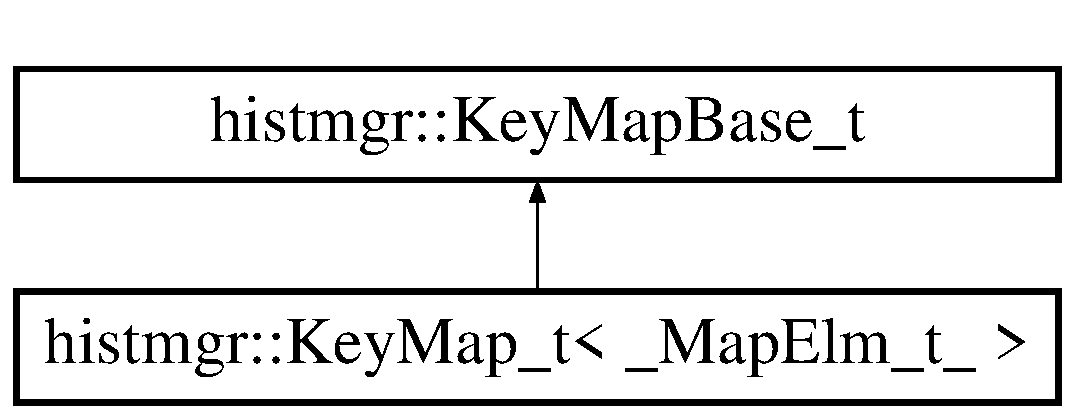
\includegraphics[height=2cm]{classhistmgr_1_1KeyMap__t}
\end{center}
\end{figure}
\subsection*{Public Types}
\begin{DoxyCompactItemize}
\item 
typedef {\bf KeyMapIterator\_\-t}$<$ \_\-MapElm\_\-t\_\- $>$ {\bfseries iterator}\label{classhistmgr_1_1KeyMap__t_a8a2d57bf4a4aa46158fdd4507348423f}

\item 
typedef {\bf KeyMapConstIterator\_\-t}$<$ \_\-MapElm\_\-t\_\- $>$ {\bfseries const\_\-iterator}\label{classhistmgr_1_1KeyMap__t_ad7d7fae50c54bcd113540b47031e1d2f}

\end{DoxyCompactItemize}
\subsection*{Public Member Functions}
\begin{DoxyCompactItemize}
\item 
bool {\bf hasKey} (const {\bf Key\_\-t} \&a\_\-key) const \label{classhistmgr_1_1KeyMap__t_aa9036fe4ff391f5b7136b9dfb4c89a1b}

\begin{DoxyCompactList}\small\item\em Check whether an element exist already for the given key. \item\end{DoxyCompactList}\item 
void {\bf assign} (const {\bf Key\_\-t} \&a\_\-key, const \_\-MapElm\_\-t\_\- \&elm)
\begin{DoxyCompactList}\small\item\em Assign an element to the given key. \item\end{DoxyCompactList}\item 
\_\-MapElm\_\-t\_\- \& {\bf operator[$\,$]} (const {\bf Key\_\-t} \&a\_\-key)
\begin{DoxyCompactList}\small\item\em Get the element assigned to the given key. \item\end{DoxyCompactList}\item 
const \_\-MapElm\_\-t\_\- \& {\bf operator[$\,$]} (const {\bf Key\_\-t} \&a\_\-key) const 
\begin{DoxyCompactList}\small\item\em Get the element assigned to the given key (read only access). \item\end{DoxyCompactList}\item 
{\bf iterator} {\bfseries begin} ()\label{classhistmgr_1_1KeyMap__t_a6ae54175e1f99ac32dc131a059c7a7ad}

\item 
{\bf iterator} {\bfseries end} ()\label{classhistmgr_1_1KeyMap__t_ac9b146e882cd7797c72b9726b0adbb70}

\item 
{\bf const\_\-iterator} {\bfseries begin} () const \label{classhistmgr_1_1KeyMap__t_a922213bbe19da6f1193bef396c145e53}

\item 
{\bf const\_\-iterator} {\bfseries end} () const \label{classhistmgr_1_1KeyMap__t_a7536d781834f271a6edb0ed965b2f286}

\end{DoxyCompactItemize}
\subsection*{Private Attributes}
\begin{DoxyCompactItemize}
\item 
std::vector$<$ \_\-MapElm\_\-t\_\- $>$ {\bfseries \_\-elmList}\label{classhistmgr_1_1KeyMap__t_a76efa9a3eceb29a7e669629d6f22538d}

\end{DoxyCompactItemize}
\subsection*{Friends}
\begin{DoxyCompactItemize}
\item 
class {\bfseries HistMgr}\label{classhistmgr_1_1KeyMap__t_a3cc85db784d7651390e41024125eb3a0}

\end{DoxyCompactItemize}


\subsection{Detailed Description}
\subsubsection*{template$<$typename \_\-MapElm\_\-t\_\-$>$ class histmgr::KeyMap\_\-t$<$ \_\-MapElm\_\-t\_\- $>$}

List of elements (KeyMap). The elements are identified by their names. A contrinuous serial number is assigned to each element. The serial number can be used to quickly access the histograms 

Definition at line 196 of file KeyMap\_\-t.hh.

\subsection{Member Function Documentation}
\index{histmgr::KeyMap\_\-t@{histmgr::KeyMap\_\-t}!assign@{assign}}
\index{assign@{assign}!histmgr::KeyMap_t@{histmgr::KeyMap\_\-t}}
\subsubsection[{assign}]{\setlength{\rightskip}{0pt plus 5cm}template$<$typename \_\-MapElm\_\-t\_\-$>$ void {\bf histmgr::KeyMap\_\-t}$<$ \_\-MapElm\_\-t\_\- $>$::assign (const {\bf Key\_\-t} \& {\em a\_\-key}, \/  const \_\-MapElm\_\-t\_\- \& {\em elm})\hspace{0.3cm}{\ttfamily  [inline]}}\label{classhistmgr_1_1KeyMap__t_a3c2c47af4647caeb9b5712f90f4d7410}


Assign an element to the given key. 
\begin{DoxyParams}{Parameters}
\item[{\em a\_\-key}]the key to which an element should be assigned. \item[{\em elm}]the element. If an element is already assigned to the key, then the old element is deleted. \end{DoxyParams}


Definition at line 221 of file KeyMap\_\-t.hh.

Referenced by histmgr::HistMgr::getOrCreatehistogramGroup(), histmgr::HistMgr::Group\_\-t::setGraphCollection(), histmgr::HistMgr::Group\_\-t::setHistogram2DCollection(), histmgr::HistMgr::Group\_\-t::setHistogramCollection(), and histmgr::HistMgr::Group\_\-t::setProfileCollection().\index{histmgr::KeyMap\_\-t@{histmgr::KeyMap\_\-t}!operator[]@{operator[]}}
\index{operator[]@{operator[]}!histmgr::KeyMap_t@{histmgr::KeyMap\_\-t}}
\subsubsection[{operator[]}]{\setlength{\rightskip}{0pt plus 5cm}template$<$typename \_\-MapElm\_\-t\_\-$>$ const \_\-MapElm\_\-t\_\-\& {\bf histmgr::KeyMap\_\-t}$<$ \_\-MapElm\_\-t\_\- $>$::operator[$\,$] (const {\bf Key\_\-t} \& {\em a\_\-key}) const\hspace{0.3cm}{\ttfamily  [inline]}}\label{classhistmgr_1_1KeyMap__t_a307a82ab48b2708d640cbc783b61a222}


Get the element assigned to the given key (read only access). 
\begin{DoxyParams}{Parameters}
\item[{\em a\_\-key}]the key of the element. \end{DoxyParams}


Definition at line 247 of file KeyMap\_\-t.hh.\index{histmgr::KeyMap\_\-t@{histmgr::KeyMap\_\-t}!operator[]@{operator[]}}
\index{operator[]@{operator[]}!histmgr::KeyMap_t@{histmgr::KeyMap\_\-t}}
\subsubsection[{operator[]}]{\setlength{\rightskip}{0pt plus 5cm}template$<$typename \_\-MapElm\_\-t\_\-$>$ \_\-MapElm\_\-t\_\-\& {\bf histmgr::KeyMap\_\-t}$<$ \_\-MapElm\_\-t\_\- $>$::operator[$\,$] (const {\bf Key\_\-t} \& {\em a\_\-key})\hspace{0.3cm}{\ttfamily  [inline]}}\label{classhistmgr_1_1KeyMap__t_a587283f7ab94b2eef10adfc1ba55dedc}


Get the element assigned to the given key. 
\begin{DoxyParams}{Parameters}
\item[{\em a\_\-key}]the key of the element. \end{DoxyParams}


Definition at line 236 of file KeyMap\_\-t.hh.

The documentation for this class was generated from the following file:\begin{DoxyCompactItemize}
\item 
KeyMap\_\-t.hh\end{DoxyCompactItemize}

\section{histmgr::KeyMapBase\_\-t Class Reference}
\label{classhistmgr_1_1KeyMapBase__t}\index{histmgr::KeyMapBase\_\-t@{histmgr::KeyMapBase\_\-t}}


Base class of the element list which only manages the name mapping.  


{\ttfamily \#include $<$KeyMap\_\-t.hh$>$}Inheritance diagram for histmgr::KeyMapBase\_\-t::\begin{figure}[H]
\begin{center}
\leavevmode
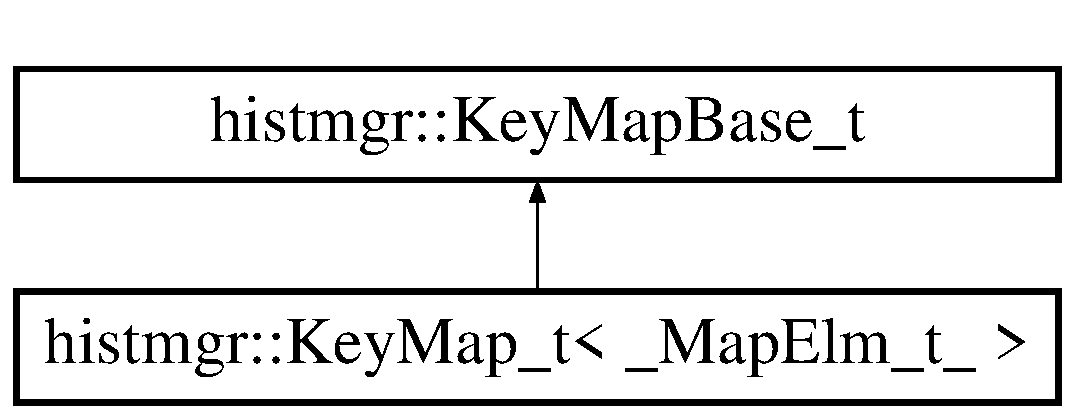
\includegraphics[height=2cm]{classhistmgr_1_1KeyMapBase__t}
\end{center}
\end{figure}
\subsection*{Public Types}
\begin{DoxyCompactItemize}
\item 
typedef std::map$<$ std::string, unsigned int $>$ {\bfseries NameMap\_\-t}\label{classhistmgr_1_1KeyMapBase__t_ae49c6a47e8e2391af4a57a3dc1f40020}

\end{DoxyCompactItemize}
\subsection*{Public Member Functions}
\begin{DoxyCompactItemize}
\item 
NameMap\_\-t::const\_\-iterator {\bfseries nameListBegin} () const \label{classhistmgr_1_1KeyMapBase__t_af1bc65af4564e7cd74c6ab25b35ca9e5}

\item 
NameMap\_\-t::const\_\-iterator {\bfseries nameListEnd} () const \label{classhistmgr_1_1KeyMapBase__t_aac7ea5403cabbabff2a01dc108072f1f}

\item 
bool {\bfseries empty} () const \label{classhistmgr_1_1KeyMapBase__t_a63938a3f927f441c92a91467eee12fa4}

\item 
unsigned int {\bfseries size} () const \label{classhistmgr_1_1KeyMapBase__t_abe4ee7508376462845afcfe84ce92672}

\end{DoxyCompactItemize}
\subsection*{Static Public Member Functions}
\begin{DoxyCompactItemize}
\item 
static {\bf Key\_\-t} {\bfseries createKey} (NameMap\_\-t::const\_\-iterator \&iter)\label{classhistmgr_1_1KeyMapBase__t_a0abfc2a6b98414d55e92a0c9c69b4b29}

\end{DoxyCompactItemize}
\subsection*{Protected Member Functions}
\begin{DoxyCompactItemize}
\item 
bool {\bf \_\-hasKey} (const {\bf Key\_\-t} \&a\_\-key) const \label{classhistmgr_1_1KeyMapBase__t_aed1d4e8444789c2f0089bec2b68a091b}

\begin{DoxyCompactList}\small\item\em Check whether an element exist already for the given key. \item\end{DoxyCompactList}\item 
bool {\bfseries \_\-insertNew} (const {\bf Key\_\-t} \&a\_\-key, unsigned int next\_\-element)\label{classhistmgr_1_1KeyMapBase__t_a8c886c4d400a0549978b170ddd846d1e}

\item 
bool {\bfseries \_\-setIndexCache} (const {\bf Key\_\-t} \&a\_\-key)\label{classhistmgr_1_1KeyMapBase__t_a51614c13e31ea6616cefd41580c92288}

\end{DoxyCompactItemize}
\subsection*{Protected Attributes}
\begin{DoxyCompactItemize}
\item 
NameMap\_\-t {\bfseries \_\-idList}\label{classhistmgr_1_1KeyMapBase__t_a759b7cd45f2bff8c5c5c83954c3f1295}

\end{DoxyCompactItemize}
\subsection*{Friends}
\begin{DoxyCompactItemize}
\item 
class {\bfseries HistMgr}\label{classhistmgr_1_1KeyMapBase__t_a3cc85db784d7651390e41024125eb3a0}

\end{DoxyCompactItemize}


\subsection{Detailed Description}
Base class of the element list which only manages the name mapping. 

Definition at line 22 of file KeyMap\_\-t.hh.

The documentation for this class was generated from the following file:\begin{DoxyCompactItemize}
\item 
KeyMap\_\-t.hh\end{DoxyCompactItemize}

\section{histmgr::KeyMapConstIterator\_\-t$<$ \_\-Map\_\-t\_\- $>$ Class Template Reference}
\label{classhistmgr_1_1KeyMapConstIterator__t}\index{histmgr::KeyMapConstIterator\_\-t@{histmgr::KeyMapConstIterator\_\-t}}


Const Iterator for the KeyMap.  


{\ttfamily \#include $<$KeyMap\_\-t.hh$>$}\subsection*{Public Member Functions}
\begin{DoxyCompactItemize}
\item 
{\bf KeyMapConstIterator\_\-t} \& {\bfseries operator++} (int)\label{classhistmgr_1_1KeyMapConstIterator__t_a836ba25c49adada842fbae460c128324}

\item 
const \_\-Map\_\-t\_\- \& {\bfseries operator$\ast$} () const \label{classhistmgr_1_1KeyMapConstIterator__t_ab5b2ed2dd09f955fac73a81ea946a279}

\item 
bool {\bfseries operator!=} (const {\bf KeyMapConstIterator\_\-t} \&a)\label{classhistmgr_1_1KeyMapConstIterator__t_a6287d9b0a5a0416e7fb7148b4e7c8d50}

\item 
bool {\bfseries operator==} (const {\bf KeyMapConstIterator\_\-t} \&a)\label{classhistmgr_1_1KeyMapConstIterator__t_a1d8772a655ce9206fc4ca55ec1180d10}

\item 
const std::string \& {\bfseries name} () const \label{classhistmgr_1_1KeyMapConstIterator__t_a177a0274749f6e1886bc635f710ee8ab}

\end{DoxyCompactItemize}
\subsection*{Data Fields}
\begin{DoxyCompactItemize}
\item 
std::map$<$ std::string, unsigned int $>$::const\_\-iterator {\bfseries \_\-iter}\label{classhistmgr_1_1KeyMapConstIterator__t_a80de00a5a879add47244319e194c550a}

\item 
std::map$<$ std::string, unsigned int $>$::const\_\-iterator {\bfseries \_\-end}\label{classhistmgr_1_1KeyMapConstIterator__t_a83ae501c29ac9a9f7fcd51d9971a9fb1}

\item 
const std::vector$<$ \_\-Map\_\-t\_\- $>$ $\ast$ {\bfseries \_\-elmListP}\label{classhistmgr_1_1KeyMapConstIterator__t_ae70832f44812b9a959ae5213f46228bf}

\end{DoxyCompactItemize}
\subsection*{Protected Member Functions}
\begin{DoxyCompactItemize}
\item 
{\bfseries KeyMapConstIterator\_\-t} (std::map$<$ std::string, unsigned int $>$::const\_\-iterator iter, std::map$<$ std::string, unsigned int $>$::const\_\-iterator end, const std::vector$<$ \_\-Map\_\-t\_\- $>$ $\ast$elm\_\-list)\label{classhistmgr_1_1KeyMapConstIterator__t_a6558bc7bfcfb2688625a19ca1638c25e}

\end{DoxyCompactItemize}
\subsection*{Friends}
\begin{DoxyCompactItemize}
\item 
class {\bfseries KeyMap\_\-t$<$ \_\-Map\_\-t\_\- $>$}\label{classhistmgr_1_1KeyMapConstIterator__t_a191ea493c1085e4505ff75fc2371f4fc}

\end{DoxyCompactItemize}


\subsection{Detailed Description}
\subsubsection*{template$<$typename \_\-Map\_\-t\_\-$>$ class histmgr::KeyMapConstIterator\_\-t$<$ \_\-Map\_\-t\_\- $>$}

Const Iterator for the KeyMap. 

Definition at line 150 of file KeyMap\_\-t.hh.

The documentation for this class was generated from the following file:\begin{DoxyCompactItemize}
\item 
KeyMap\_\-t.hh\end{DoxyCompactItemize}

\section{histmgr::KeyMapIterator\_\-t$<$ \_\-Map\_\-t\_\- $>$ Class Template Reference}
\label{classhistmgr_1_1KeyMapIterator__t}\index{histmgr::KeyMapIterator\_\-t@{histmgr::KeyMapIterator\_\-t}}


Iterator for the KeyMap.  


{\ttfamily \#include $<$KeyMap\_\-t.hh$>$}\subsection*{Public Member Functions}
\begin{DoxyCompactItemize}
\item 
{\bf KeyMapIterator\_\-t} \& {\bfseries operator++} (int)\label{classhistmgr_1_1KeyMapIterator__t_a8dcf109b5967c4c11f0e52d4aef777f3}

\item 
\_\-Map\_\-t\_\- \& {\bfseries operator$\ast$} ()\label{classhistmgr_1_1KeyMapIterator__t_a33664e3b5550d2fdd286f1669efa7d10}

\item 
const \_\-Map\_\-t\_\- \& {\bfseries operator$\ast$} () const \label{classhistmgr_1_1KeyMapIterator__t_af5a8d583bcf26ff7866df066d200598e}

\item 
bool {\bfseries operator!=} (const {\bf KeyMapIterator\_\-t} \&a)\label{classhistmgr_1_1KeyMapIterator__t_ae02f2c50b69107f3eb9b31a9828560f8}

\item 
bool {\bfseries operator==} (const {\bf KeyMapIterator\_\-t} \&a)\label{classhistmgr_1_1KeyMapIterator__t_aef04b811fd364003d920e2af59ef58f2}

\item 
const std::string \& {\bfseries name} () const \label{classhistmgr_1_1KeyMapIterator__t_ad4fc569584ae74eeed57ad051f243e9a}

\end{DoxyCompactItemize}
\subsection*{Data Fields}
\begin{DoxyCompactItemize}
\item 
std::map$<$ std::string, unsigned int $>$::const\_\-iterator {\bfseries \_\-iter}\label{classhistmgr_1_1KeyMapIterator__t_aa41ef843e1366530672421aa495ba594}

\item 
std::map$<$ std::string, unsigned int $>$::const\_\-iterator {\bfseries \_\-end}\label{classhistmgr_1_1KeyMapIterator__t_a219ddf2712319da91557d603dc2e1a4d}

\item 
std::vector$<$ \_\-Map\_\-t\_\- $>$ $\ast$ {\bfseries \_\-elmListP}\label{classhistmgr_1_1KeyMapIterator__t_a7ab18ad834c26291af97185dd417d07a}

\end{DoxyCompactItemize}
\subsection*{Protected Member Functions}
\begin{DoxyCompactItemize}
\item 
{\bfseries KeyMapIterator\_\-t} (std::map$<$ std::string, unsigned int $>$::const\_\-iterator iter, std::map$<$ std::string, unsigned int $>$::const\_\-iterator end, std::vector$<$ \_\-Map\_\-t\_\- $>$ $\ast$elm\_\-list)\label{classhistmgr_1_1KeyMapIterator__t_a3612ff6f41ef33520d8bab59f38c4ed5}

\end{DoxyCompactItemize}
\subsection*{Friends}
\begin{DoxyCompactItemize}
\item 
class {\bfseries KeyMap\_\-t$<$ \_\-Map\_\-t\_\- $>$}\label{classhistmgr_1_1KeyMapIterator__t_a191ea493c1085e4505ff75fc2371f4fc}

\end{DoxyCompactItemize}


\subsection{Detailed Description}
\subsubsection*{template$<$typename \_\-Map\_\-t\_\-$>$ class histmgr::KeyMapIterator\_\-t$<$ \_\-Map\_\-t\_\- $>$}

Iterator for the KeyMap. 

Definition at line 99 of file KeyMap\_\-t.hh.

The documentation for this class was generated from the following file:\begin{DoxyCompactItemize}
\item 
KeyMap\_\-t.hh\end{DoxyCompactItemize}

\section{marlin::TBTrackRemover::LCEventModifier Class Reference}
\label{classmarlin_1_1TBTrackRemover_1_1LCEventModifier}\index{marlin::TBTrackRemover::LCEventModifier@{marlin::TBTrackRemover::LCEventModifier}}


Helper class to for the modification of the Event Header.  
\subsection*{Static Public Member Functions}
\begin{DoxyCompactItemize}
\item 
static void {\bfseries deleteCollection} (LCEvent $\ast$r, const std::string \&name)\label{classmarlin_1_1TBTrackRemover_1_1LCEventModifier_adac30a804a963f47f0da9dff12be6a12}

\end{DoxyCompactItemize}


\subsection{Detailed Description}
Helper class to for the modification of the Event Header. 

Definition at line 72 of file TBTrackRemover.hh.

The documentation for this class was generated from the following file:\begin{DoxyCompactItemize}
\item 
TBTrackRemover.hh\end{DoxyCompactItemize}

\section{LCPayload$<$ Payload $>$ Class Template Reference}
\label{classLCPayload}\index{LCPayload@{LCPayload}}


Specific LCIO implementation of the interface to store generic user data.  


{\ttfamily \#include $<$LCPayload.hh$>$}\subsection*{Public Member Functions}
\begin{DoxyCompactItemize}
\item 
{\bf LCPayload} ()\label{classLCPayload_a8b8d145b1753cabef13f6da15d957c39}

\begin{DoxyCompactList}\small\item\em Constructors. \item\end{DoxyCompactList}\item 
{\bfseries LCPayload} (const EVENT::LCGenericObject $\ast$obj)\label{classLCPayload_abecb2b247eb9265510f784db83297806}

\item 
{\bfseries LCPayload} (const Payload \&c)\label{classLCPayload_a96860b56042d95ba0c4fa36aeef8c164}

\item 
{\bfseries LCPayload} (const Payload \&p, IMPL::LCGenericObjectImpl \&obj)\label{classLCPayload_aa29b1863b733b5e544696fa29788f9c2}

\item 
virtual {\bf $\sim$LCPayload} ()\label{classLCPayload_ac1e66fabe1f9f65972ec738f7574e84c}

\begin{DoxyCompactList}\small\item\em Destructor. \item\end{DoxyCompactList}\item 
virtual void {\bf update} (const EVENT::LCGenericObject $\ast$obj)\label{classLCPayload_a461543886a17454a20f92d685f8c8bdc}

\begin{DoxyCompactList}\small\item\em Update values within the object from an LCGenericObject. \item\end{DoxyCompactList}\item 
virtual EVENT::LCGenericObject $\ast$ {\bf output} () const \label{classLCPayload_a438b42bdc529adc71a5c0bc960b32883}

\begin{DoxyCompactList}\small\item\em Create a new LCGenericObject and fill it. \item\end{DoxyCompactList}\item 
virtual void {\bf update} (const std::string \&fileName)\label{classLCPayload_a5fce76c90beebf958604253586bfd649}

\begin{DoxyCompactList}\small\item\em Update values within the object from a flat file. \item\end{DoxyCompactList}\item 
virtual void {\bf output} (const std::string \&fileName) const \label{classLCPayload_a891246b9b47aa64690632308f9af7a15}

\begin{DoxyCompactList}\small\item\em Create a new flat file and fill it. \item\end{DoxyCompactList}\item 
virtual int {\bf getNInt} () const \label{classLCPayload_a60bf414fbb56e82a7a8a405023f263b7}

\begin{DoxyCompactList}\small\item\em Number of integer values stored in this object. \item\end{DoxyCompactList}\item 
virtual int {\bf getNFloat} () const \label{classLCPayload_adb8d459967c8cbd5e349cf0ceb233d1b}

\begin{DoxyCompactList}\small\item\em Number of float values stored in this object. \item\end{DoxyCompactList}\item 
virtual int {\bf getNDouble} () const \label{classLCPayload_ab465cc9ebd35f82089fa980470eca413}

\begin{DoxyCompactList}\small\item\em Number of double values stored in this object. \item\end{DoxyCompactList}\item 
virtual int {\bf getIntVal} (int index) const \label{classLCPayload_a470d04e59dca5e575292f46170bc01d1}

\begin{DoxyCompactList}\small\item\em Returns the integer value for the given index. \item\end{DoxyCompactList}\item 
virtual float {\bf getFloatVal} (int index) const \label{classLCPayload_a051df316ec7a181e623643adf9748c48}

\begin{DoxyCompactList}\small\item\em Returns the float value for the given index. \item\end{DoxyCompactList}\item 
virtual double {\bf getDoubleVal} (int index) const \label{classLCPayload_a6752bc94c3be02a767eae41599c2c663}

\begin{DoxyCompactList}\small\item\em Returns the double value for the given index. \item\end{DoxyCompactList}\item 
virtual void {\bf setIntVal} (unsigned index, int value)\label{classLCPayload_aa50e9b8b87d51d6482aa312348981448}

\begin{DoxyCompactList}\small\item\em Sets the integer value at the given index. \item\end{DoxyCompactList}\item 
virtual void {\bf setFloatVal} (unsigned index, float value)\label{classLCPayload_a12e1b5355c7a8a06bb2a6057a709c75a}

\begin{DoxyCompactList}\small\item\em Sets the float value at the given index. \item\end{DoxyCompactList}\item 
virtual void {\bf setDoubleVal} (unsigned index, double value)\label{classLCPayload_a4d93cf109f053a0fd493c4989082f663}

\begin{DoxyCompactList}\small\item\em Sets the double value at the given index. \item\end{DoxyCompactList}\item 
virtual bool {\bf isFixedSize} () const \label{classLCPayload_ac693f8e406129f62f897e30272ef1f9b}

\begin{DoxyCompactList}\small\item\em True if objects of the implementation class have a fixed size, i.e getNInt, getNFloat and getNDouble will return values that are constant during the lifetime of the object. \item\end{DoxyCompactList}\item 
virtual const std::string {\bf getTypeName} () const \label{classLCPayload_a7338d24c98c4aa99a5d720477e8301fa}

\begin{DoxyCompactList}\small\item\em The type name of the user class (typically the class name). \item\end{DoxyCompactList}\item 
virtual const std::string {\bf getDataDescription} () const 
\begin{DoxyCompactList}\small\item\em The description string. \item\end{DoxyCompactList}\item 
virtual const Payload \& {\bf constants} () const \label{classLCPayload_a9893dcd67b1d2483e48fcb437aa0b29c}

\begin{DoxyCompactList}\small\item\em Access the actual data for read or write. \item\end{DoxyCompactList}\item 
virtual void {\bfseries constants} (const Payload \&p)\label{classLCPayload_a6396d80f22ca663e914843d438338b35}

\item 
virtual const Payload \& {\bfseries payload} () const \label{classLCPayload_a153acaff49e7286ae3514867bb8032c6}

\item 
virtual void {\bfseries payload} (const Payload \&p)\label{classLCPayload_ac51c5e8c33b60d49403b9326f61ff475}

\end{DoxyCompactItemize}
\subsection*{Protected Attributes}
\begin{DoxyCompactItemize}
\item 
Payload {\bfseries \_\-payload}\label{classLCPayload_a281072ee5a8fe9247b7ed45915236907}

\end{DoxyCompactItemize}


\subsection{Detailed Description}
\subsubsection*{template$<$class Payload$>$ class LCPayload$<$ Payload $>$}

Specific LCIO implementation of the interface to store generic user data. \begin{DoxyAuthor}{Author}
dauncey 
\end{DoxyAuthor}
\begin{DoxyVersion}{Version}

\end{DoxyVersion}
Id}
\doxyref{LCPayload.hh}{p.}{LCPayload_8hh_source},v 1.3 2009-\/03-\/24 11:40:43 dauncey Exp 

Definition at line 19 of file LCPayload.hh.

\subsection{Member Function Documentation}
\index{LCPayload@{LCPayload}!getDataDescription@{getDataDescription}}
\index{getDataDescription@{getDataDescription}!LCPayload@{LCPayload}}
\subsubsection[{getDataDescription}]{\setlength{\rightskip}{0pt plus 5cm}template$<$class Payload $>$ const std::string {\bf LCPayload}$<$ Payload $>$::getDataDescription () const\hspace{0.3cm}{\ttfamily  [inline, virtual]}}\label{classLCPayload_a118d95b1a2c431153cc3691d29b18692}


The description string. A comma separated list of pairs of type identifier, one of 'i','f','d' followed by ':' and an attribute name, e.g. \char`\"{}i:cellId,f:offset,f:gain\char`\"{}. 

Definition at line 342 of file LCPayload.hh.

The documentation for this class was generated from the following file:\begin{DoxyCompactItemize}
\item 
LCPayload.hh\end{DoxyCompactItemize}

\section{marlin::RunInfoProcessor::LCRunModifier Class Reference}
\label{classmarlin_1_1RunInfoProcessor_1_1LCRunModifier}\index{marlin::RunInfoProcessor::LCRunModifier@{marlin::RunInfoProcessor::LCRunModifier}}


Helper class to for the modification of the Run Header.  
\subsection*{Static Public Member Functions}
\begin{DoxyCompactItemize}
\item 
static void {\bfseries setRun} (LCRunHeader $\ast$r, int n, std::string description)\label{classmarlin_1_1RunInfoProcessor_1_1LCRunModifier_ad5b4d3ac8439c98e21d6ec66de4ec8ab}

\end{DoxyCompactItemize}


\subsection{Detailed Description}
Helper class to for the modification of the Run Header. 

Definition at line 159 of file RunInfoProcessor.hh.

The documentation for this class was generated from the following file:\begin{DoxyCompactItemize}
\item 
RunInfoProcessor.hh\end{DoxyCompactItemize}

\section{LCTrackPayload$<$ Payload $>$ Class Template Reference}
\label{classLCTrackPayload}\index{LCTrackPayload@{LCTrackPayload}}


Specific LCIO implementation of the interface to store generic user data.  


{\ttfamily \#include $<$LCTrackPayload.hh$>$}\subsection*{Public Member Functions}
\begin{DoxyCompactItemize}
\item 
{\bf LCTrackPayload} ()\label{classLCTrackPayload_a10aabc99033fe1163ec4bacd1f683e52}

\begin{DoxyCompactList}\small\item\em Constructors. \item\end{DoxyCompactList}\item 
{\bfseries LCTrackPayload} (const EVENT::LCGenericObject $\ast$obj)\label{classLCTrackPayload_a995d11dd83d9e9f10c2c178425ab96dc}

\item 
{\bfseries LCTrackPayload} (const Payload \&c)\label{classLCTrackPayload_ac7283dc42793904ea2e6a61ad47e760f}

\item 
{\bfseries LCTrackPayload} (const Payload \&p, IMPL::LCGenericObjectImpl \&obj)\label{classLCTrackPayload_a64e99cf37fab6f26835ee47464379444}

\item 
virtual {\bf $\sim$LCTrackPayload} ()\label{classLCTrackPayload_a76b84074f0064c45f8473662820d481d}

\begin{DoxyCompactList}\small\item\em Destructor. \item\end{DoxyCompactList}\item 
virtual void {\bf update} (const EVENT::LCGenericObject $\ast$obj)\label{classLCTrackPayload_aea1a5317f1a5abd198c127638c2505da}

\begin{DoxyCompactList}\small\item\em Update values within the object from an LCGenericObject. \item\end{DoxyCompactList}\item 
virtual EVENT::LCGenericObject $\ast$ {\bf output} () const \label{classLCTrackPayload_ad6359058eb2c59c82b10ca98fa90424a}

\begin{DoxyCompactList}\small\item\em Create a new LCGenericObject and fill it. \item\end{DoxyCompactList}\item 
virtual int {\bf getNInt} () const \label{classLCTrackPayload_ac6ce3cdeab53d7c8c098279a9598f3c1}

\begin{DoxyCompactList}\small\item\em Number of integer values stored in this object. \item\end{DoxyCompactList}\item 
virtual int {\bf getNFloat} () const \label{classLCTrackPayload_a1eb3d42fd2ac6eac76dd2b0c76c54689}

\begin{DoxyCompactList}\small\item\em Number of float values stored in this object. \item\end{DoxyCompactList}\item 
virtual int {\bf getNDouble} () const \label{classLCTrackPayload_a8c5dfa41f6430205758fa8eb30868771}

\begin{DoxyCompactList}\small\item\em Number of double values stored in this object. \item\end{DoxyCompactList}\item 
virtual int {\bf getIntVal} (int index) const \label{classLCTrackPayload_a4f6dc00e5a78eb37534c29545efad2d7}

\begin{DoxyCompactList}\small\item\em Returns the integer value for the given index. \item\end{DoxyCompactList}\item 
virtual float {\bf getFloatVal} (int index) const \label{classLCTrackPayload_a47c0f1771fcfb56e86941c90449f88c8}

\begin{DoxyCompactList}\small\item\em Returns the float value for the given index. \item\end{DoxyCompactList}\item 
virtual double {\bf getDoubleVal} (int index) const \label{classLCTrackPayload_a7d2682a798e967dd00363dc90a1b1dcc}

\begin{DoxyCompactList}\small\item\em Returns the double value for the given index. \item\end{DoxyCompactList}\item 
virtual void {\bf setIntVal} (unsigned index, int value)\label{classLCTrackPayload_a4e92e7bfa326b29e1bc0bb8888d700e1}

\begin{DoxyCompactList}\small\item\em Sets the integer value at the given index. \item\end{DoxyCompactList}\item 
virtual void {\bf setFloatVal} (unsigned index, float value)\label{classLCTrackPayload_ad92a24649bec4959158a57f709a35423}

\begin{DoxyCompactList}\small\item\em Sets the float value at the given index. \item\end{DoxyCompactList}\item 
virtual void {\bf setDoubleVal} (unsigned index, double value)\label{classLCTrackPayload_a23161fdc6b57a9fcd4d3a900bd333310}

\begin{DoxyCompactList}\small\item\em Sets the double value at the given index. \item\end{DoxyCompactList}\item 
virtual bool {\bf isFixedSize} () const \label{classLCTrackPayload_aabc45cbe4ecf99f2031378c9cedfc804}

\begin{DoxyCompactList}\small\item\em True if objects of the implementation class have a fixed size, i.e getNInt, getNFloat and getNDouble will return values that are constant during the lifetime of the object. \item\end{DoxyCompactList}\item 
virtual const std::string {\bf getTypeName} () const \label{classLCTrackPayload_ab56a3408c7013b69adf621b0813fbbf9}

\begin{DoxyCompactList}\small\item\em The type name of the user class (typically the class name). \item\end{DoxyCompactList}\item 
virtual const std::string {\bf getDataDescription} () const 
\begin{DoxyCompactList}\small\item\em The description string. \item\end{DoxyCompactList}\item 
virtual const Payload \& {\bf constants} () const \label{classLCTrackPayload_a1d0364cf45deb6c764ffecbe08e0cf84}

\begin{DoxyCompactList}\small\item\em Access the actual data for read or write. \item\end{DoxyCompactList}\item 
virtual void {\bfseries constants} (const Payload \&p)\label{classLCTrackPayload_a572f1162e50700b9f241e7ba0d80219f}

\item 
virtual const Payload \& {\bfseries payload} () const \label{classLCTrackPayload_a65557857fdc305d92c0e99b740effa9e}

\item 
virtual void {\bfseries payload} (const Payload \&p)\label{classLCTrackPayload_ab78efc5558a8c4a60776f37ce9a3982a}

\end{DoxyCompactItemize}
\subsection*{Protected Attributes}
\begin{DoxyCompactItemize}
\item 
Payload {\bfseries \_\-payload}\label{classLCTrackPayload_a89353b7b9de237aa375f1a7a94e59ad7}

\end{DoxyCompactItemize}


\subsection{Detailed Description}
\subsubsection*{template$<$class Payload$>$ class LCTrackPayload$<$ Payload $>$}

Specific LCIO implementation of the interface to store generic user data. \begin{DoxyAuthor}{Author}
dauncey 
\end{DoxyAuthor}
\begin{DoxyVersion}{Version}

\end{DoxyVersion}
Id}
\doxyref{LCTrackPayload.hh}{p.}{LCTrackPayload_8hh_source},v 1.1 2007-\/04-\/26 14:34:28 poeschl Exp 

Definition at line 19 of file LCTrackPayload.hh.

\subsection{Member Function Documentation}
\index{LCTrackPayload@{LCTrackPayload}!getDataDescription@{getDataDescription}}
\index{getDataDescription@{getDataDescription}!LCTrackPayload@{LCTrackPayload}}
\subsubsection[{getDataDescription}]{\setlength{\rightskip}{0pt plus 5cm}template$<$class Payload $>$ const std::string {\bf LCTrackPayload}$<$ Payload $>$::getDataDescription () const\hspace{0.3cm}{\ttfamily  [inline, virtual]}}\label{classLCTrackPayload_acad8e51a5ce7ccd79dc652c03177f091}


The description string. A comma separated list of pairs of type identifier, one of 'i','f','d' followed by ':' and an attribute name, e.g. \char`\"{}i:cellId,f:offset,f:gain\char`\"{}. 

Definition at line 252 of file LCTrackPayload.hh.

The documentation for this class was generated from the following file:\begin{DoxyCompactItemize}
\item 
LCTrackPayload.hh\end{DoxyCompactItemize}

\section{TBTrack::LinearFitResult Class Reference}
\label{classTBTrack_1_1LinearFitResult}\index{TBTrack::LinearFitResult@{TBTrack::LinearFitResult}}
\subsection*{Public Member Functions}
\begin{DoxyCompactItemize}
\item 
{\bfseries LinearFitResult} (double c, int n, const TVectorD \&p, const TMatrixDSym \&e)\label{classTBTrack_1_1LinearFitResult_a3e4ba61e44c68bcf81db05f704d5d5b1}

\item 
double {\bfseries chiSquared} () const \label{classTBTrack_1_1LinearFitResult_a036042e6787c607d0ee51b20044d52b9}

\item 
int {\bfseries numberOfDof} () const \label{classTBTrack_1_1LinearFitResult_ab41a070ef6c6e60a04f44e1ad833caa3}

\item 
double {\bfseries probability} () const \label{classTBTrack_1_1LinearFitResult_a750253e1904b159bee301eceb5f09f80}

\item 
const TVectorD \& {\bfseries parameters} () const \label{classTBTrack_1_1LinearFitResult_ae0ed921b62f6653de3531a406335c7c2}

\item 
const TMatrixDSym \& {\bfseries errors} () const \label{classTBTrack_1_1LinearFitResult_aaef15bed0282bc3f5e8e2e59f0d611d6}

\item 
double {\bfseries probability} (const TVectorD \&p) const \label{classTBTrack_1_1LinearFitResult_a1fa9bf5b974dd4a0bc5d692c66bd820b}

\item 
std::ostream \& {\bfseries print} (std::ostream \&o=std::cout, const std::string \&s=\char`\"{}\char`\"{}) const \label{classTBTrack_1_1LinearFitResult_adafd249c515c0a59daa63513c7a5fb1c}

\end{DoxyCompactItemize}
\subsection*{Private Attributes}
\begin{DoxyCompactItemize}
\item 
double {\bfseries \_\-chiSquared}\label{classTBTrack_1_1LinearFitResult_a009140f1916c5f9fffbdde89e000fe94}

\item 
int {\bfseries \_\-numberOfDof}\label{classTBTrack_1_1LinearFitResult_a2a4b4553ede2fc2363e4beab085404c8}

\item 
TVectorD {\bfseries \_\-parameters}\label{classTBTrack_1_1LinearFitResult_aab3a876556b7afa7eb0492e30a51b56d}

\item 
TMatrixDSym {\bfseries \_\-errors}\label{classTBTrack_1_1LinearFitResult_a71acc0645f990d05042ccd962cf36ef7}

\end{DoxyCompactItemize}


\subsection{Detailed Description}


Definition at line 15 of file LinearFitResult.hh.

The documentation for this class was generated from the following files:\begin{DoxyCompactItemize}
\item 
LinearFitResult.hh\item 
LinearFitResult.cc\end{DoxyCompactItemize}

\section{TBTrack::LinearFitter Class Reference}
\label{classTBTrack_1_1LinearFitter}\index{TBTrack::LinearFitter@{TBTrack::LinearFitter}}
\subsection*{Public Member Functions}
\begin{DoxyCompactItemize}
\item 
void {\bfseries fitInitialisation} (const TMatrixD \&z, const TMatrixDSym \&e)\label{classTBTrack_1_1LinearFitter_af83e617778ace54723fba9d11eaad900}

\item 
const TMatrixDSym \& {\bfseries errorMatrix} () const \label{classTBTrack_1_1LinearFitter_ab3c00a9eb140ba63e0cae20e7db9df43}

\item 
const TMatrixD \& {\bfseries solutionMatrix} () const \label{classTBTrack_1_1LinearFitter_adb053f46cd4b1cabd89aafb802b14b4e}

\item 
const TMatrixDSym \& {\bfseries chiSquaredMatrix} () const \label{classTBTrack_1_1LinearFitter_a941c09f4b9d2976aa9b14ac1c9d55ccd}

\item 
std::ostream \& {\bfseries printInitialisation} (std::ostream \&o=std::cout, const std::string \&s=\char`\"{}\char`\"{}) const \label{classTBTrack_1_1LinearFitter_a458de2b57f0b458e007fab1eb04a3b71}

\item 
{\bf LinearFitResult} {\bfseries fitResult} (const TVectorD \&x) const \label{classTBTrack_1_1LinearFitter_a3609570379fc6b194cd8a576d5579be6}

\end{DoxyCompactItemize}
\subsection*{Private Attributes}
\begin{DoxyCompactItemize}
\item 
TMatrixD {\bfseries \_\-fitValues}\label{classTBTrack_1_1LinearFitter_a0d5ab614c1263e593037ebdd7fccf92d}

\item 
TMatrixDSym {\bfseries \_\-errorMatrix}\label{classTBTrack_1_1LinearFitter_a92f10ab1b7cc02975e9c84823e93af18}

\item 
TMatrixD {\bfseries \_\-solutionMatrix}\label{classTBTrack_1_1LinearFitter_af166aa8136a2aa0f60f47fa2e984f2cd}

\item 
TMatrixDSym {\bfseries \_\-chiSquaredMatrix}\label{classTBTrack_1_1LinearFitter_a86f7868c45931d0cc11e150bb81761c4}

\end{DoxyCompactItemize}


\subsection{Detailed Description}


Definition at line 15 of file LinearFitter.hh.

The documentation for this class was generated from the following files:\begin{DoxyCompactItemize}
\item 
LinearFitter.hh\item 
LinearFitter.cc\end{DoxyCompactItemize}

\section{TBTrack::MapConstants Class Reference}
\label{classTBTrack_1_1MapConstants}\index{TBTrack::MapConstants@{TBTrack::MapConstants}}
\subsection*{Public Types}
\begin{DoxyCompactItemize}
\item 
enum \{ {\bfseries numberOfInts} = 1
 \}
\item 
enum \{ {\bfseries numberOfFloats} = 0
 \}
\item 
enum \{ {\bfseries numberOfDoubles} = 0
 \}
\end{DoxyCompactItemize}
\subsection*{Public Member Functions}
\begin{DoxyCompactItemize}
\item 
{\bfseries MapConstants} (int p=0)\label{classTBTrack_1_1MapConstants_ad6a908a71ad6e73996a27429b7ba4485}

\item 
std::ostream \& {\bfseries print} (std::ostream \&o=std::cout, const std::string \&s=\char`\"{}\char`\"{}) const \label{classTBTrack_1_1MapConstants_abf0ecdc32902053ca7bacf7ab68d6166}

\item 
const int $\ast$ {\bfseries intData} () const \label{classTBTrack_1_1MapConstants_aeaffabb97fe13e54bca6a2ccfcf5dcf4}

\item 
int $\ast$ {\bfseries intData} ()\label{classTBTrack_1_1MapConstants_a64090ab098d7b42996eb37ac0181c6d9}

\item 
const float $\ast$ {\bfseries floatData} () const \label{classTBTrack_1_1MapConstants_a5db3dc38042fe8bc9fd1346eddbf2b43}

\item 
float $\ast$ {\bfseries floatData} ()\label{classTBTrack_1_1MapConstants_a25791641151a9a929d1cc7d9cb080976}

\item 
const double $\ast$ {\bfseries doubleData} () const \label{classTBTrack_1_1MapConstants_a2dc86123f3989ad6f8e633aacec4c918}

\item 
double $\ast$ {\bfseries doubleData} ()\label{classTBTrack_1_1MapConstants_a0b3f2db804b686ebd71e35d718564853}

\end{DoxyCompactItemize}
\subsection*{Private Attributes}
\begin{DoxyCompactItemize}
\item 
int {\bfseries \_\-period}\label{classTBTrack_1_1MapConstants_a136a931938bf1830db32ecd17745e4a5}

\end{DoxyCompactItemize}


\subsection{Detailed Description}


Definition at line 12 of file MapConstants.hh.

The documentation for this class was generated from the following files:\begin{DoxyCompactItemize}
\item 
MapConstants.hh\item 
MapConstants.cc\end{DoxyCompactItemize}

\section{marlin::MCRunTimeProcessor Class Reference}
\label{classmarlin_1_1MCRunTimeProcessor}\index{marlin::MCRunTimeProcessor@{marlin::MCRunTimeProcessor}}
\subsection*{Public Member Functions}
\begin{DoxyCompactItemize}
\item 
virtual Processor $\ast$ {\bfseries newProcessor} ()\label{classmarlin_1_1MCRunTimeProcessor_afaa7a8f8af2e6d40734992523adb0f18}

\item 
virtual const std::string \& {\bfseries name} () const \label{classmarlin_1_1MCRunTimeProcessor_a594976d07353672f85e23f50bc2c0183}

\item 
virtual void {\bfseries modifyEvent} (LCEvent $\ast$evt)\label{classmarlin_1_1MCRunTimeProcessor_a51c9d9bf4f8b66e2c3b82f31f0f26bba}

\item 
virtual void {\bfseries init} ()\label{classmarlin_1_1MCRunTimeProcessor_a645e036d00d0ac4f016a6fb8d33f40c1}

\item 
virtual void {\bfseries processRunHeader} (LCRunHeader $\ast$run)\label{classmarlin_1_1MCRunTimeProcessor_a94ffb5e4ec27a97de5a30bc5c43f0655}

\item 
virtual void {\bfseries check} (LCEvent $\ast$evt)\label{classmarlin_1_1MCRunTimeProcessor_afcac2282e9028e447afc453cb0f3cc5d}

\item 
virtual void {\bfseries end} ()\label{classmarlin_1_1MCRunTimeProcessor_a1b72a2ae28eb11cf4460b765a0ef0e01}

\end{DoxyCompactItemize}
\subsection*{Private Attributes}
\begin{DoxyCompactItemize}
\item 
std::string {\bfseries \_\-dbInit}\label{classmarlin_1_1MCRunTimeProcessor_a4e743478c041ee93d3256134520e3c49}

\item 
std::string {\bfseries \_\-folderRunTime}\label{classmarlin_1_1MCRunTimeProcessor_a30df635002d96b32291813aa3f91d585}

\item 
std::string {\bfseries \_\-folderLocation}\label{classmarlin_1_1MCRunTimeProcessor_a2be1163f77699025a223cd1ebb1040f4}

\item 
RunLocationWhizard $\ast$ {\bfseries \_\-runlocationwhizard}\label{classmarlin_1_1MCRunTimeProcessor_a29bd192e54ae09e3b3dd9240b2f7ac23}

\item 
RunTimeWhizard $\ast$ {\bfseries \_\-runtimewhizard}\label{classmarlin_1_1MCRunTimeProcessor_a136eebf08c52e00b691e7ad562ebae76}

\item 
int {\bfseries \_\-runNumber}\label{classmarlin_1_1MCRunTimeProcessor_a9e3dea800b1c0e2104a00a5007714ddd}

\item 
int {\bfseries \_\-savetyMargin}\label{classmarlin_1_1MCRunTimeProcessor_ae97bf35ad864f1bafba1864de9d03bc5}

\item 
UTIL::LCTime {\bfseries \_\-eventTime}\label{classmarlin_1_1MCRunTimeProcessor_a119971e6c2b38d2ff99240191f82ce09}

\end{DoxyCompactItemize}


\subsection{Detailed Description}


Definition at line 18 of file MCRunTimeProcessor.hh.

The documentation for this class was generated from the following files:\begin{DoxyCompactItemize}
\item 
MCRunTimeProcessor.hh\item 
MCRunTimeProcessor.cc\end{DoxyCompactItemize}

\section{CALICE::MipSelect Class Reference}
\label{classCALICE_1_1MipSelect}\index{CALICE::MipSelect@{CALICE::MipSelect}}


Simple class to try to select hits resulting from one mip.  


{\ttfamily \#include $<$MipSelect.hh$>$}\subsection*{Public Member Functions}
\begin{DoxyCompactItemize}
\item 
Processor $\ast$ {\bfseries newProcessor} ()\label{classCALICE_1_1MipSelect_a0f4980cc56e6302a351f1029f1259655}

\item 
{\bf MipSelect} ()
\begin{DoxyCompactList}\small\item\em Select Mips . \item\end{DoxyCompactList}\item 
void {\bf init} ()
\begin{DoxyCompactList}\small\item\em Called at the begin of the job before anything is read. \item\end{DoxyCompactList}\item 
void {\bf processRunHeader} (LCRunHeader $\ast$run)
\begin{DoxyCompactList}\small\item\em Called for every run, e.g. \item\end{DoxyCompactList}\item 
void {\bf processEvent} (LCEvent $\ast$evtP)\label{classCALICE_1_1MipSelect_a4fda653147df06d659939dfe36aceb34}

\begin{DoxyCompactList}\small\item\em Called for every event -\/ the working horse. \item\end{DoxyCompactList}\item 
void {\bfseries end} ()\label{classCALICE_1_1MipSelect_aa1e14b5e9e444acae637f2cbcc0511e0}

\end{DoxyCompactItemize}
\subsection*{Protected Attributes}
\begin{DoxyCompactItemize}
\item 
IntVec {\bf \_\-nHits}
\begin{DoxyCompactList}\small\item\em minimum and maximum required number of hits for a cluster (Marlin processor parameter). \item\end{DoxyCompactList}\item 
Float\_\-t {\bf \_\-maxDist}
\begin{DoxyCompactList}\small\item\em the maximum distance between hits considered to be close (Marlin processor parameter). \item\end{DoxyCompactList}\item 
FloatVec {\bf \_\-clusterEnergy}
\begin{DoxyCompactList}\small\item\em minimum and maximum required cluster energy (Marlin processor parameter). \item\end{DoxyCompactList}\item 
Float\_\-t {\bf \_\-maxChi2}
\begin{DoxyCompactList}\small\item\em minimum required chi2 of the x and y straight line fits (Marlin processor parameter). \item\end{DoxyCompactList}\item 
Float\_\-t {\bf \_\-w0}
\begin{DoxyCompactList}\small\item\em Cut parameter which defines the energy threshold of hits considered in the centre-\/of-\/gravity determination (Marlin processor parameter). \item\end{DoxyCompactList}\item 
FloatVec {\bf \_\-posError}
\begin{DoxyCompactList}\small\item\em Error assigned to the cluster barycentre (marlin processor parameter). \item\end{DoxyCompactList}\item 
std::string {\bf \_\-colName}\label{classCALICE_1_1MipSelect_ac9ae37843e4f13fdb0339917b36e3bb9}

\begin{DoxyCompactList}\small\item\em name of the hit input collection (Marlin processor parameter) \item\end{DoxyCompactList}\item 
std::string {\bf \_\-clusterColName}\label{classCALICE_1_1MipSelect_ad9094c81faee001d8cb848cbd0da5ac4}

\begin{DoxyCompactList}\small\item\em name of the cluster output collection (Marlin processor parameter) \item\end{DoxyCompactList}\end{DoxyCompactItemize}
\subsection*{Private Attributes}
\begin{DoxyCompactItemize}
\item 
std::vector$<$ UInt\_\-t $>$ {\bf \_\-isolatedHits}\label{classCALICE_1_1MipSelect_a9e44a652e454927b32108da491368eec}

\begin{DoxyCompactList}\small\item\em temporary buffer \item\end{DoxyCompactList}\end{DoxyCompactItemize}


\subsection{Detailed Description}
Simple class to try to select hits resulting from one mip. This processor tries to find hits in the chosen hit collection which are close together. If the number adjacent hits is large enough a cluster is created. \begin{Desc}
\item[{\bf Todo}]: add shower shape criterium, maximum number of tolerated hits \end{Desc}


Definition at line 28 of file MipSelect.hh.

\subsection{Constructor \& Destructor Documentation}
\index{CALICE::MipSelect@{CALICE::MipSelect}!MipSelect@{MipSelect}}
\index{MipSelect@{MipSelect}!CALICE::MipSelect@{CALICE::MipSelect}}
\subsubsection[{MipSelect}]{\setlength{\rightskip}{0pt plus 5cm}CALICE::MipSelect::MipSelect ()}\label{classCALICE_1_1MipSelect_a187a4421470be1e416ad1aaffabdab45}


Select Mips . Mip tracks are search within the calorimeter hits. Developped for cosmics. 

Definition at line 42 of file MipSelect.cc.

References \_\-clusterColName, \_\-clusterEnergy, \_\-colName, \_\-maxChi2, \_\-maxDist, \_\-nHits, \_\-posError, and \_\-w0.

\subsection{Member Function Documentation}
\index{CALICE::MipSelect@{CALICE::MipSelect}!init@{init}}
\index{init@{init}!CALICE::MipSelect@{CALICE::MipSelect}}
\subsubsection[{init}]{\setlength{\rightskip}{0pt plus 5cm}void CALICE::MipSelect::init ()}\label{classCALICE_1_1MipSelect_a6e9d97e8a6a621de6803dac121a9662b}


Called at the begin of the job before anything is read. Use to initialize the processor, e.g. book histograms. 

Definition at line 176 of file MipSelect.cc.

References \_\-clusterEnergy, and \_\-nHits.\index{CALICE::MipSelect@{CALICE::MipSelect}!processRunHeader@{processRunHeader}}
\index{processRunHeader@{processRunHeader}!CALICE::MipSelect@{CALICE::MipSelect}}
\subsubsection[{processRunHeader}]{\setlength{\rightskip}{0pt plus 5cm}void CALICE::MipSelect::processRunHeader (LCRunHeader $\ast$ {\em run})\hspace{0.3cm}{\ttfamily  [inline]}}\label{classCALICE_1_1MipSelect_af4ddc35f44aa0c65145e592fba7abb64}


Called for every run, e.g. overwrite to initialize run dependent histograms. 

Definition at line 46 of file MipSelect.hh.

\subsection{Field Documentation}
\index{CALICE::MipSelect@{CALICE::MipSelect}!\_\-clusterEnergy@{\_\-clusterEnergy}}
\index{\_\-clusterEnergy@{\_\-clusterEnergy}!CALICE::MipSelect@{CALICE::MipSelect}}
\subsubsection[{\_\-clusterEnergy}]{\setlength{\rightskip}{0pt plus 5cm}FloatVec {\bf CALICE::MipSelect::\_\-clusterEnergy}\hspace{0.3cm}{\ttfamily  [protected]}}\label{classCALICE_1_1MipSelect_a4724ccf37d271a114791a2d0d5575cb9}


minimum and maximum required cluster energy (Marlin processor parameter). 

Definition at line 57 of file MipSelect.hh.

Referenced by init(), MipSelect(), and processEvent().\index{CALICE::MipSelect@{CALICE::MipSelect}!\_\-maxChi2@{\_\-maxChi2}}
\index{\_\-maxChi2@{\_\-maxChi2}!CALICE::MipSelect@{CALICE::MipSelect}}
\subsubsection[{\_\-maxChi2}]{\setlength{\rightskip}{0pt plus 5cm}Float\_\-t {\bf CALICE::MipSelect::\_\-maxChi2}\hspace{0.3cm}{\ttfamily  [protected]}}\label{classCALICE_1_1MipSelect_a9ad0ff3988f10698ba6398158fdba7d3}


minimum required chi2 of the x and y straight line fits (Marlin processor parameter). 

Definition at line 58 of file MipSelect.hh.

Referenced by MipSelect(), and processEvent().\index{CALICE::MipSelect@{CALICE::MipSelect}!\_\-maxDist@{\_\-maxDist}}
\index{\_\-maxDist@{\_\-maxDist}!CALICE::MipSelect@{CALICE::MipSelect}}
\subsubsection[{\_\-maxDist}]{\setlength{\rightskip}{0pt plus 5cm}Float\_\-t {\bf CALICE::MipSelect::\_\-maxDist}\hspace{0.3cm}{\ttfamily  [protected]}}\label{classCALICE_1_1MipSelect_af5b5c0952ac42edf3e33ccc3354ce999}


the maximum distance between hits considered to be close (Marlin processor parameter). 

Definition at line 56 of file MipSelect.hh.

Referenced by MipSelect(), and processEvent().\index{CALICE::MipSelect@{CALICE::MipSelect}!\_\-nHits@{\_\-nHits}}
\index{\_\-nHits@{\_\-nHits}!CALICE::MipSelect@{CALICE::MipSelect}}
\subsubsection[{\_\-nHits}]{\setlength{\rightskip}{0pt plus 5cm}IntVec {\bf CALICE::MipSelect::\_\-nHits}\hspace{0.3cm}{\ttfamily  [protected]}}\label{classCALICE_1_1MipSelect_a9942825c9ee70c394f78dde00c43c8ef}


minimum and maximum required number of hits for a cluster (Marlin processor parameter). 

Definition at line 55 of file MipSelect.hh.

Referenced by init(), MipSelect(), and processEvent().\index{CALICE::MipSelect@{CALICE::MipSelect}!\_\-posError@{\_\-posError}}
\index{\_\-posError@{\_\-posError}!CALICE::MipSelect@{CALICE::MipSelect}}
\subsubsection[{\_\-posError}]{\setlength{\rightskip}{0pt plus 5cm}FloatVec {\bf CALICE::MipSelect::\_\-posError}\hspace{0.3cm}{\ttfamily  [protected]}}\label{classCALICE_1_1MipSelect_a47f1821c1518e00d403d026c5b1eb848}


Error assigned to the cluster barycentre (marlin processor parameter). 

Definition at line 62 of file MipSelect.hh.

Referenced by MipSelect(), and processEvent().\index{CALICE::MipSelect@{CALICE::MipSelect}!\_\-w0@{\_\-w0}}
\index{\_\-w0@{\_\-w0}!CALICE::MipSelect@{CALICE::MipSelect}}
\subsubsection[{\_\-w0}]{\setlength{\rightskip}{0pt plus 5cm}Float\_\-t {\bf CALICE::MipSelect::\_\-w0}\hspace{0.3cm}{\ttfamily  [protected]}}\label{classCALICE_1_1MipSelect_ae601de1184f473e69224607d827436a3}


Cut parameter which defines the energy threshold of hits considered in the centre-\/of-\/gravity determination (Marlin processor parameter). 

Definition at line 59 of file MipSelect.hh.

Referenced by MipSelect(), and processEvent().

The documentation for this class was generated from the following files:\begin{DoxyCompactItemize}
\item 
MipSelect.hh\item 
MipSelect.cc\end{DoxyCompactItemize}

\section{CALICE::ModuleIndexReverseLookup Class Reference}
\label{classCALICE_1_1ModuleIndexReverseLookup}\index{CALICE::ModuleIndexReverseLookup@{CALICE::ModuleIndexReverseLookup}}


Creates huge arrays which allows to find out the module and the cell index using the Mokka conform geometrical index.  


{\ttfamily \#include $<$ModuleIndexReverseLookup.hh$>$}\subsection*{Public Member Functions}
\begin{DoxyCompactItemize}
\item 
void {\bf createIndexReverseLookup} (const MappingAndAlignment \&mapping)
\begin{DoxyCompactList}\small\item\em Create a huge arrays which contains for each cell the module and the cell index. \item\end{DoxyCompactList}\item 
pair$<$ UInt\_\-t, UInt\_\-t $>$ {\bf getModuleAndCellIndex} (const MappingAndAlignment \&mapping, const CellIndex \&a\_\-cell\_\-index) const 
\begin{DoxyCompactList}\small\item\em Return the module and cell index for the given Mokka conform geometrical cell index. \item\end{DoxyCompactList}\end{DoxyCompactItemize}
\subsection*{Protected Types}
\begin{DoxyCompactItemize}
\item 
typedef {\bf SimpleArray\_\-t}$<$ {\bf SimpleArray\_\-t}$<$ {\bf SimpleArray\_\-t}$<$ {\bf SimpleArray\_\-t}$<$ unsigned short $>$ $>$ $>$ $>$ {\bfseries CellIndexArray\_\-t}\label{classCALICE_1_1ModuleIndexReverseLookup_a3cb8a61f3dc239ac5ffbee685bf6988f}

\end{DoxyCompactItemize}
\subsection*{Protected Attributes}
\begin{DoxyCompactItemize}
\item 
{\bf SimpleArray\_\-t}$<$ {\bf SimpleArray\_\-t}$<$ {\bf SimpleArray\_\-t}$<$ unsigned short $>$ $>$ $>$ {\bf \_\-moduleIndexArray}
\begin{DoxyCompactList}\small\item\em Array which contains for each layer and wafer row and column the module index. \item\end{DoxyCompactList}\item 
{\bf SimpleArray\_\-t}$<$ {\bf CellIndexArray\_\-t} $>$ {\bf \_\-moduleTypeArray}
\begin{DoxyCompactList}\small\item\em Array which contains for each module type the cell indices for a pad of a given wafer, pad row and column. \item\end{DoxyCompactList}\end{DoxyCompactItemize}


\subsection{Detailed Description}
Creates huge arrays which allows to find out the module and the cell index using the Mokka conform geometrical index. 

Definition at line 9 of file ModuleIndexReverseLookup.hh.

\subsection{Member Function Documentation}
\index{CALICE::ModuleIndexReverseLookup@{CALICE::ModuleIndexReverseLookup}!createIndexReverseLookup@{createIndexReverseLookup}}
\index{createIndexReverseLookup@{createIndexReverseLookup}!CALICE::ModuleIndexReverseLookup@{CALICE::ModuleIndexReverseLookup}}
\subsubsection[{createIndexReverseLookup}]{\setlength{\rightskip}{0pt plus 5cm}void CALICE::ModuleIndexReverseLookup::createIndexReverseLookup (const MappingAndAlignment \& {\em mapping})}\label{classCALICE_1_1ModuleIndexReverseLookup_a2bd62812d099ee99ec7cd26c8e25b39c}


Create a huge arrays which contains for each cell the module and the cell index. The array which contains the cell indices uses the module type, the wafer and pad row and column indices. The array which contains the module indices uses the wafer row and column index. 

Definition at line 10 of file ModuleIndexReverseLookup.cc.

References \_\-moduleIndexArray, and \_\-moduleTypeArray.\index{CALICE::ModuleIndexReverseLookup@{CALICE::ModuleIndexReverseLookup}!getModuleAndCellIndex@{getModuleAndCellIndex}}
\index{getModuleAndCellIndex@{getModuleAndCellIndex}!CALICE::ModuleIndexReverseLookup@{CALICE::ModuleIndexReverseLookup}}
\subsubsection[{getModuleAndCellIndex}]{\setlength{\rightskip}{0pt plus 5cm}pair$<$UInt\_\-t, UInt\_\-t$>$ CALICE::ModuleIndexReverseLookup::getModuleAndCellIndex (const MappingAndAlignment \& {\em mapping}, \/  const CellIndex \& {\em a\_\-cell\_\-index}) const\hspace{0.3cm}{\ttfamily  [inline]}}\label{classCALICE_1_1ModuleIndexReverseLookup_a639f10b89a671e6259c9e2d3ae98965f}


Return the module and cell index for the given Mokka conform geometrical cell index. 
\begin{DoxyParams}{Parameters}
\item[{\em mapping}]reference to the mapping object. \item[{\em a\_\-cell\_\-index}]the Mokka conform geometrical cell index \end{DoxyParams}
\begin{DoxyReturn}{Returns}
the module index and the cell index on the module. The module index is the index in the list of defined module locations (coditions datae). The cell index is the index of the cells on the module. The pads are multiplexed on 12(6) lines (readout chips). First the 12(6) cells of the fist sample are stored than the cells of next sample. 
\end{DoxyReturn}


ifdef BOUNDARY\_\-CHECK 

Definition at line 31 of file ModuleIndexReverseLookup.hh.

References \_\-moduleIndexArray, and \_\-moduleTypeArray.

Referenced by CALICE::HoldScanAnalysis::processEvent().

\subsection{Field Documentation}
\index{CALICE::ModuleIndexReverseLookup@{CALICE::ModuleIndexReverseLookup}!\_\-moduleIndexArray@{\_\-moduleIndexArray}}
\index{\_\-moduleIndexArray@{\_\-moduleIndexArray}!CALICE::ModuleIndexReverseLookup@{CALICE::ModuleIndexReverseLookup}}
\subsubsection[{\_\-moduleIndexArray}]{\setlength{\rightskip}{0pt plus 5cm}{\bf SimpleArray\_\-t}$<$ {\bf SimpleArray\_\-t}$<$ {\bf SimpleArray\_\-t}$<$ unsigned short $>$ $>$ $>$ {\bf CALICE::ModuleIndexReverseLookup::\_\-moduleIndexArray}\hspace{0.3cm}{\ttfamily  [protected]}}\label{classCALICE_1_1ModuleIndexReverseLookup_a6f4c66de3a572faa169b6d8f605e7e2f}


Array which contains for each layer and wafer row and column the module index. 

Definition at line 81 of file ModuleIndexReverseLookup.hh.

Referenced by createIndexReverseLookup(), and getModuleAndCellIndex().\index{CALICE::ModuleIndexReverseLookup@{CALICE::ModuleIndexReverseLookup}!\_\-moduleTypeArray@{\_\-moduleTypeArray}}
\index{\_\-moduleTypeArray@{\_\-moduleTypeArray}!CALICE::ModuleIndexReverseLookup@{CALICE::ModuleIndexReverseLookup}}
\subsubsection[{\_\-moduleTypeArray}]{\setlength{\rightskip}{0pt plus 5cm}{\bf SimpleArray\_\-t}$<$ {\bf CellIndexArray\_\-t} $>$ {\bf CALICE::ModuleIndexReverseLookup::\_\-moduleTypeArray}\hspace{0.3cm}{\ttfamily  [protected]}}\label{classCALICE_1_1ModuleIndexReverseLookup_a26cc1c3d8dba383ba59b4a8e8b96c98d}


Array which contains for each module type the cell indices for a pad of a given wafer, pad row and column. 

Definition at line 86 of file ModuleIndexReverseLookup.hh.

Referenced by createIndexReverseLookup(), and getModuleAndCellIndex().

The documentation for this class was generated from the following files:\begin{DoxyCompactItemize}
\item 
ModuleIndexReverseLookup.hh\item 
ModuleIndexReverseLookup.cc\end{DoxyCompactItemize}

\section{CALICE::IntegratedHcalProcessor::NeighbourItem Struct Reference}
\label{structCALICE_1_1IntegratedHcalProcessor_1_1NeighbourItem}\index{CALICE::IntegratedHcalProcessor::NeighbourItem@{CALICE::IntegratedHcalProcessor::NeighbourItem}}


int \_\-fudgeNonExistingSaturationCorrections;  


{\ttfamily \#include $<$IntegratedHcalProcessor.hh$>$}\subsection*{Data Fields}
\begin{DoxyCompactItemize}
\item 
unsigned short {\bfseries module}\label{structCALICE_1_1IntegratedHcalProcessor_1_1NeighbourItem_a222785cbd28eaf736340eef25e436e20}

\item 
unsigned short {\bfseries cellkey}\label{structCALICE_1_1IntegratedHcalProcessor_1_1NeighbourItem_a145ab8e4188b4e065424e61b1281dbdb}

\item 
float {\bfseries weight}\label{structCALICE_1_1IntegratedHcalProcessor_1_1NeighbourItem_a9c688d0bbc8c74d9a8403c0d8f12f0f6}

\end{DoxyCompactItemize}


\subsection{Detailed Description}
int \_\-fudgeNonExistingSaturationCorrections; bool \_\-correctSatLY;

float \_\-lightyield[HCAL\_\-N\_\-MOD+1][HCAL\_\-N\_\-CELL]; float \_\-lightyieldError[HCAL\_\-N\_\-MOD+1][HCAL\_\-N\_\-CELL]; 

Definition at line 168 of file IntegratedHcalProcessor.hh.

The documentation for this struct was generated from the following file:\begin{DoxyCompactItemize}
\item 
IntegratedHcalProcessor.hh\end{DoxyCompactItemize}

\section{CALICE::NoiseParameter Class Reference}
\label{classCALICE_1_1NoiseParameter}\index{CALICE::NoiseParameter@{CALICE::NoiseParameter}}


Information about a pad: Pedestal, noise, etc.  


{\ttfamily \#include $<$NoiseParameter.hh$>$}\subsection*{Public Types}
\begin{DoxyCompactItemize}
\item 
enum \{ {\bfseries numberOfInts} = 4
 \}
\item 
enum \{ {\bfseries numberOfFloats} = 0
 \}
\item 
enum \{ {\bfseries numberOfDoubles} = 7
 \}
\end{DoxyCompactItemize}
\subsection*{Public Member Functions}
\begin{DoxyCompactItemize}
\item 
{\bfseries NoiseParameter} (int cellID0, int module\_\-index, int cell\_\-index, double noise, double pedestal)\label{classCALICE_1_1NoiseParameter_a5ae8a2eda536c5234c898a1fed313103}

\item 
{\bfseries NoiseParameter} (int cellID0, int module\_\-index, int cell\_\-index)\label{classCALICE_1_1NoiseParameter_adf999180ff627b662343e5069db133d7}

\item 
{\bfseries NoiseParameter} (int module\_\-index, int cell\_\-index)\label{classCALICE_1_1NoiseParameter_ac3ad7f004d153853a1e2a800a4018e29}

\item 
void {\bf setPedestal} (double aPedestal)\label{classCALICE_1_1NoiseParameter_a1b356206a293f69bf1ed40d27ecb818b}

\begin{DoxyCompactList}\small\item\em Set the pedestal. \item\end{DoxyCompactList}\item 
double {\bf getPedestal} () const \label{classCALICE_1_1NoiseParameter_adb7a5b09ba13a4f638df6d60b59c9587}

\begin{DoxyCompactList}\small\item\em Get the pedestal. \item\end{DoxyCompactList}\item 
void {\bf setPedestalBeforeSIC} (double aOld\_\-pedestal)\label{classCALICE_1_1NoiseParameter_a3388d4aae5f8d532667b38ac4e9af8a6}

\begin{DoxyCompactList}\small\item\em Set the pedestal before Signal Induced Corrections are applied. \item\end{DoxyCompactList}\item 
void {\bf setPedestalBeforeGC} (double aOld\_\-pedestal)\label{classCALICE_1_1NoiseParameter_ab20b21bb8db009637332f8b15471fc7f}

\begin{DoxyCompactList}\small\item\em Set the pedestal before Global Corrections are applied. \item\end{DoxyCompactList}\item 
double {\bf getPedestalBeforeSIC} () const \label{classCALICE_1_1NoiseParameter_a8aa648b980a102191797e806bec1fe1b}

\begin{DoxyCompactList}\small\item\em Get the pedestal before Signal Induced Corrections are applied. \item\end{DoxyCompactList}\item 
double {\bf getPedestalBeforeGC} () const \label{classCALICE_1_1NoiseParameter_a2075113211efc4ce905ad6698775b9ed}

\begin{DoxyCompactList}\small\item\em Get the pedestal before Global Corrections are applied. \item\end{DoxyCompactList}\item 
void {\bf setNoise} (double aNoise)\label{classCALICE_1_1NoiseParameter_aa887925f83397f287cad1cf77f5beb5f}

\begin{DoxyCompactList}\small\item\em Set the noise. \item\end{DoxyCompactList}\item 
void {\bfseries setCoherentNoise} (double aCohNoise)\label{classCALICE_1_1NoiseParameter_a8cab49decf1acc0c958d8b2c4f4135ce}

\item 
void {\bfseries setNoiseBeforeSIC} (double aOld\_\-noise)\label{classCALICE_1_1NoiseParameter_ac4acc09827523e318148775dc1334fdb}

\item 
void {\bfseries setNoiseBeforeGC} (double aOld\_\-noise)\label{classCALICE_1_1NoiseParameter_a2db1c2d78cea0327da44aea672a846a4}

\item 
double {\bf getNoise} () const 
\begin{DoxyCompactList}\small\item\em Get the noise. \item\end{DoxyCompactList}\item 
double {\bfseries getCoherentNoise} () const \label{classCALICE_1_1NoiseParameter_a5a63ace1e424cac33ceccc67d15625b9}

\item 
double {\bfseries getNoiseBeforeSIC} () const \label{classCALICE_1_1NoiseParameter_a070e69c9ab4182aff016923bccd1e0f8}

\item 
double {\bfseries getNoiseBeforeGC} () const \label{classCALICE_1_1NoiseParameter_a92bc44cb2669afeffc46dbbc297c8891}

\item 
short {\bf isDead} () const \label{classCALICE_1_1NoiseParameter_aaad737204e2573e3fb934bb9ef373107}

\begin{DoxyCompactList}\small\item\em Return kTRUE if the pad is considered to be dead. \item\end{DoxyCompactList}\item 
void {\bf setDead} (short is\_\-dead=1)
\begin{DoxyCompactList}\small\item\em Declare the pad to be dead (or revive pad (is\_\-dead=0). \item\end{DoxyCompactList}\item 
void {\bfseries setModuleIndex} (unsigned int aModule\_\-index)\label{classCALICE_1_1NoiseParameter_a4ec1782980dd013e8f361c32f9280fad}

\item 
unsigned int {\bf getModuleIndex} () const 
\begin{DoxyCompactList}\small\item\em Get the ModuleIndex. \item\end{DoxyCompactList}\item 
void {\bf setCellIndex} (unsigned int aCell\_\-index)\label{classCALICE_1_1NoiseParameter_a6de76912e4150b4ce0b63688be1de595}

\begin{DoxyCompactList}\small\item\em Set the CellIndex. \item\end{DoxyCompactList}\item 
unsigned int {\bf getCellIndex} () const 
\begin{DoxyCompactList}\small\item\em Get the CellIndex. \item\end{DoxyCompactList}\item 
void {\bf setGeomCellIndex} (int aCellID0)\label{classCALICE_1_1NoiseParameter_a7a85f45d0e5d9bfcd07574f0ffa4ce2d}

\begin{DoxyCompactList}\small\item\em Get and set the Mokka-\/like geometrical index. \item\end{DoxyCompactList}\item 
int {\bfseries getGeomCellIndex} () const \label{classCALICE_1_1NoiseParameter_a2e5ecdf5faaddbdf33001f4ca61c5b62}

\item 
const int $\ast$ {\bfseries intData} () const \label{classCALICE_1_1NoiseParameter_ab49c24a64e65f2233dcde0c1eec61781}

\item 
int $\ast$ {\bfseries intData} ()\label{classCALICE_1_1NoiseParameter_a70ec4f6c64502b5db07d3ea74c2e46dd}

\item 
const float $\ast$ {\bfseries floatData} () const \label{classCALICE_1_1NoiseParameter_a43e6abb3eb0f278e4ec8b6f0a7b91ca2}

\item 
float $\ast$ {\bfseries floatData} ()\label{classCALICE_1_1NoiseParameter_a5044799613596b5e3547e2c9e01e9098}

\item 
const double $\ast$ {\bfseries doubleData} () const \label{classCALICE_1_1NoiseParameter_a17f9f7964cbde3a5b67bfcac3412dd23}

\item 
double $\ast$ {\bfseries doubleData} ()\label{classCALICE_1_1NoiseParameter_ad770a3fe04039177f6913d9490d1443e}

\end{DoxyCompactItemize}
\subsection*{Private Attributes}
\begin{DoxyCompactItemize}
\item 
int {\bfseries \_\-isDead}\label{classCALICE_1_1NoiseParameter_a03f4de43745541be50a09781b8e89839}

\item 
int {\bfseries \_\-moduleIndex}\label{classCALICE_1_1NoiseParameter_a6a940aaa8b66a7bc9eb0153733c42b86}

\item 
int {\bfseries \_\-cellIndex}\label{classCALICE_1_1NoiseParameter_a2c43ce031c49e48559f6aa01c6836012}

\item 
int {\bfseries \_\-cellID0}\label{classCALICE_1_1NoiseParameter_ad617a135ebfd7e49a17101d2911b06fc}

\item 
double {\bfseries \_\-pedestalBeforeGC}\label{classCALICE_1_1NoiseParameter_a84581448f67828307fda00d2cfd39c85}

\item 
double {\bfseries \_\-noiseBeforeGC}\label{classCALICE_1_1NoiseParameter_af097bce79566b82d2e920439cfd94cd1}

\item 
double {\bfseries \_\-pedestalBeforeSIC}\label{classCALICE_1_1NoiseParameter_af7aa0d50c9a7656f7e4965e9dabfa1bd}

\item 
double {\bfseries \_\-noiseBeforeSIC}\label{classCALICE_1_1NoiseParameter_ac554d0afad408a3aed8e3a521ee8c466}

\item 
double {\bfseries \_\-pedestal}\label{classCALICE_1_1NoiseParameter_a6b4a80837d89299a9319157aab127a28}

\item 
double {\bfseries \_\-noise}\label{classCALICE_1_1NoiseParameter_a48f6d0c4bc54f23e4e58df5da2bcc5f4}

\item 
double {\bfseries \_\-cohnoise}\label{classCALICE_1_1NoiseParameter_ae362643e5670037960a664be7d8c4635}

\end{DoxyCompactItemize}


\subsection{Detailed Description}
Information about a pad: Pedestal, noise, etc. This class hold the pedestal, the noise, and a flag which indicates whether the pad is considered to be dead, in function of the geometrical indices. It will be used by both data and MC 

Definition at line 12 of file NoiseParameter.hh.

\subsection{Member Function Documentation}
\index{CALICE::NoiseParameter@{CALICE::NoiseParameter}!getCellIndex@{getCellIndex}}
\index{getCellIndex@{getCellIndex}!CALICE::NoiseParameter@{CALICE::NoiseParameter}}
\subsubsection[{getCellIndex}]{\setlength{\rightskip}{0pt plus 5cm}unsigned int CALICE::NoiseParameter::getCellIndex () const}\label{classCALICE_1_1NoiseParameter_affdf12ec2ffea77fcb05ffd16e26d48a}


Get the CellIndex. The result is undefined before the CellIndexs and the noise are calculated. 

Definition at line 173 of file NoiseParameter.cc.\index{CALICE::NoiseParameter@{CALICE::NoiseParameter}!getModuleIndex@{getModuleIndex}}
\index{getModuleIndex@{getModuleIndex}!CALICE::NoiseParameter@{CALICE::NoiseParameter}}
\subsubsection[{getModuleIndex}]{\setlength{\rightskip}{0pt plus 5cm}unsigned int CALICE::NoiseParameter::getModuleIndex () const}\label{classCALICE_1_1NoiseParameter_af2c390e2f9d1c9973961045e444e6120}


Get the ModuleIndex. The result is undefined before the ModuleIndexs and the noise are calculated. 

Definition at line 165 of file NoiseParameter.cc.\index{CALICE::NoiseParameter@{CALICE::NoiseParameter}!getNoise@{getNoise}}
\index{getNoise@{getNoise}!CALICE::NoiseParameter@{CALICE::NoiseParameter}}
\subsubsection[{getNoise}]{\setlength{\rightskip}{0pt plus 5cm}double CALICE::NoiseParameter::getNoise () const}\label{classCALICE_1_1NoiseParameter_a25c5efb36b96a6d55f475d7721585d87}


Get the noise. The result is undefined before the pedestals and the noise are calculated. 

Definition at line 139 of file NoiseParameter.cc.

Referenced by CALICE::CalibrateAndApplyThreshold::processEvent().\index{CALICE::NoiseParameter@{CALICE::NoiseParameter}!setDead@{setDead}}
\index{setDead@{setDead}!CALICE::NoiseParameter@{CALICE::NoiseParameter}}
\subsubsection[{setDead}]{\setlength{\rightskip}{0pt plus 5cm}void CALICE::NoiseParameter::setDead (short {\em is\_\-dead} = {\ttfamily 1})}\label{classCALICE_1_1NoiseParameter_acb1d520b046f2365c182a492540a6881}


Declare the pad to be dead (or revive pad (is\_\-dead=0). 1=dead, 2=bad, 3=disconnected 

Definition at line 156 of file NoiseParameter.cc.

Referenced by CALICE::SimpleHitSearch::searchHits().

The documentation for this class was generated from the following files:\begin{DoxyCompactItemize}
\item 
NoiseParameter.hh\item 
NoiseParameter.cc\end{DoxyCompactItemize}

\section{NoOpCalibration Class Reference}
\label{classNoOpCalibration}\index{NoOpCalibration@{NoOpCalibration}}


Lazy calibration class.  


{\ttfamily \#include $<$NoOpCalibration.hh$>$}Inheritance diagram for NoOpCalibration::\begin{figure}[H]
\begin{center}
\leavevmode
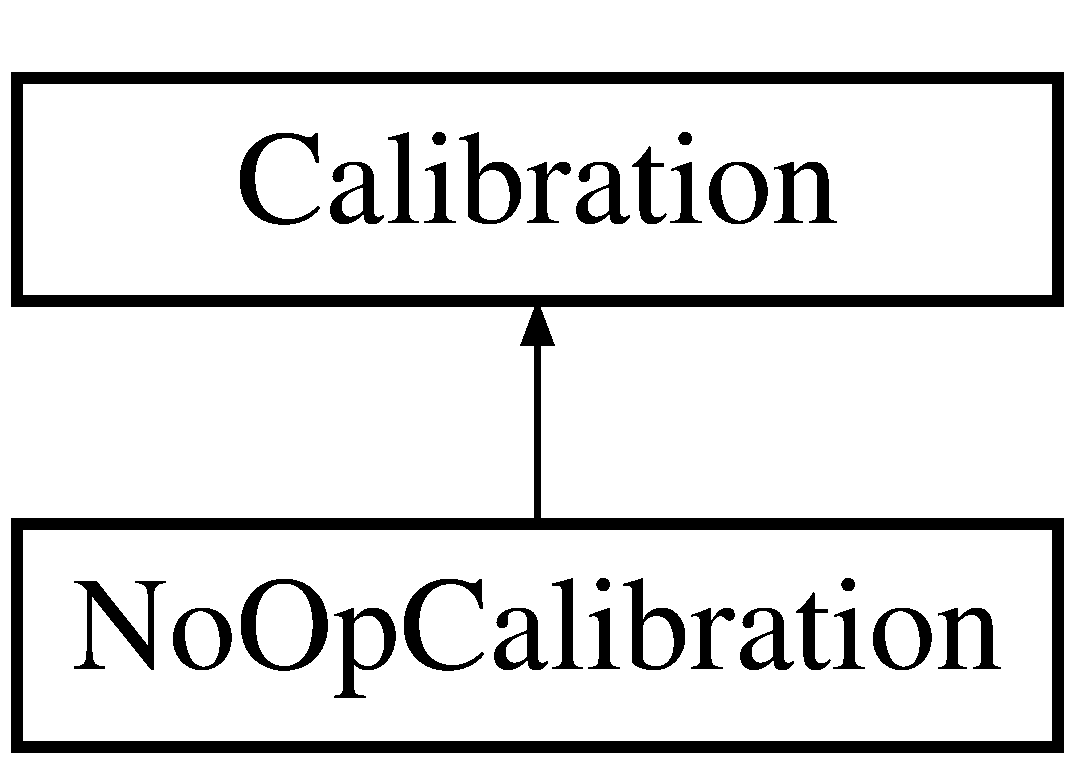
\includegraphics[height=2cm]{classNoOpCalibration}
\end{center}
\end{figure}
\subsection*{Public Member Functions}
\begin{DoxyCompactItemize}
\item 
Float\_\-t {\bf getCalibratedValue} (UInt\_\-t module\_\-index, UInt\_\-t module\_\-type, UInt\_\-t cell\_\-index, Float\_\-t adc\_\-value) const 
\begin{DoxyCompactList}\small\item\em Determine from a pedestal subtracted ADC value a calibrated value which are identical for this very lazy calibrator. \item\end{DoxyCompactList}\item 
Bool\_\-t {\bf checkForCalibrationConstantsOfModule} (UInt\_\-t module\_\-id, UInt\_\-t module\_\-type, UInt\_\-t n\_\-cells) const 
\begin{DoxyCompactList}\small\item\em Verify that calibration constants exist for a certain module. \item\end{DoxyCompactList}\item 
Int\_\-t {\bf getMiniumADCForMipThreshold} (Float\_\-t mip\_\-energy\_\-fraction) const 
\begin{DoxyCompactList}\small\item\em Get the minimum adc value mips will have for the given energy fraction on all pads. \item\end{DoxyCompactList}\end{DoxyCompactItemize}


\subsection{Detailed Description}
Lazy calibration class. Does nothing. 

Definition at line 10 of file NoOpCalibration.hh.

\subsection{Member Function Documentation}
\index{NoOpCalibration@{NoOpCalibration}!checkForCalibrationConstantsOfModule@{checkForCalibrationConstantsOfModule}}
\index{checkForCalibrationConstantsOfModule@{checkForCalibrationConstantsOfModule}!NoOpCalibration@{NoOpCalibration}}
\subsubsection[{checkForCalibrationConstantsOfModule}]{\setlength{\rightskip}{0pt plus 5cm}Bool\_\-t NoOpCalibration::checkForCalibrationConstantsOfModule (UInt\_\-t {\em module\_\-id}, \/  UInt\_\-t {\em module\_\-type}, \/  UInt\_\-t {\em n\_\-cells}) const\hspace{0.3cm}{\ttfamily  [inline, virtual]}}\label{classNoOpCalibration_acdb31ec76cef7720c0cda5fb15ffa2fb}


Verify that calibration constants exist for a certain module. 
\begin{DoxyParams}{Parameters}
\item[{\em module\_\-id}]id Or serial number of a module which uniquely identifies a detector module of a certain type. \item[{\em module\_\-type}]the type of the detector module \item[{\em n\_\-cells}]the number of cells on this module. Return true if calibration constants exist for the given module and the number of cells matches the number of calibration constants. \end{DoxyParams}


Implements {\bf Calibration} \doxyref{}{p.}{classCalibration_a04c8f21c6e77cd3c91c858ca2c9373c4}.

Definition at line 28 of file NoOpCalibration.hh.\index{NoOpCalibration@{NoOpCalibration}!getCalibratedValue@{getCalibratedValue}}
\index{getCalibratedValue@{getCalibratedValue}!NoOpCalibration@{NoOpCalibration}}
\subsubsection[{getCalibratedValue}]{\setlength{\rightskip}{0pt plus 5cm}Float\_\-t NoOpCalibration::getCalibratedValue (UInt\_\-t {\em module\_\-index}, \/  UInt\_\-t {\em module\_\-type}, \/  UInt\_\-t {\em cell\_\-index}, \/  Float\_\-t {\em adc\_\-value}) const\hspace{0.3cm}{\ttfamily  [inline, virtual]}}\label{classNoOpCalibration_a8dd43819c4e5bb09e097f4db360a57fe}


Determine from a pedestal subtracted ADC value a calibrated value which are identical for this very lazy calibrator. 
\begin{DoxyParams}{Parameters}
\item[{\em module\_\-index}]index of the module a module is considered to be a unit which is always calibrated in one calibration run. \item[{\em module\_\-type}]the type of the detector module \item[{\em cell\_\-index}]\item[{\em adc\_\-value}]the ADC value which should be calibrated. \end{DoxyParams}


Implements {\bf Calibration} \doxyref{}{p.}{classCalibration_aca88d93a445ba3021c05dd61b293568c}.

Definition at line 20 of file NoOpCalibration.hh.\index{NoOpCalibration@{NoOpCalibration}!getMiniumADCForMipThreshold@{getMiniumADCForMipThreshold}}
\index{getMiniumADCForMipThreshold@{getMiniumADCForMipThreshold}!NoOpCalibration@{NoOpCalibration}}
\subsubsection[{getMiniumADCForMipThreshold}]{\setlength{\rightskip}{0pt plus 5cm}Int\_\-t NoOpCalibration::getMiniumADCForMipThreshold (Float\_\-t {\em mip\_\-energy\_\-fraction}) const\hspace{0.3cm}{\ttfamily  [inline, virtual]}}\label{classNoOpCalibration_a8b478c6680b5980c2b87cedc8a589989}


Get the minimum adc value mips will have for the given energy fraction on all pads. 
\begin{DoxyParams}{Parameters}
\item[{\em mip\_\-energy\_\-fraction}]the energy in mips \end{DoxyParams}
\begin{DoxyReturn}{Returns}
minimum adc value which is below the given energy on all pads. This method can be used to get the lowest adc value a mip of the given energy fraction will have on all pads. This value is useful to select candidates before actually performing th calibration. This function is intended to be called at the beginning of each event. 
\end{DoxyReturn}


Implements {\bf Calibration} \doxyref{}{p.}{classCalibration_a4e45f1eca0d4fdf19ad76b8f581aee12}.

Definition at line 38 of file NoOpCalibration.hh.

The documentation for this class was generated from the following file:\begin{DoxyCompactItemize}
\item 
NoOpCalibration.hh\end{DoxyCompactItemize}

\section{NoOpCalibrationKit Class Reference}
\label{classNoOpCalibrationKit}\index{NoOpCalibrationKit@{NoOpCalibrationKit}}


Create a calibration object which just returns the uncalibrated values.  
Inheritance diagram for NoOpCalibrationKit::\begin{figure}[H]
\begin{center}
\leavevmode
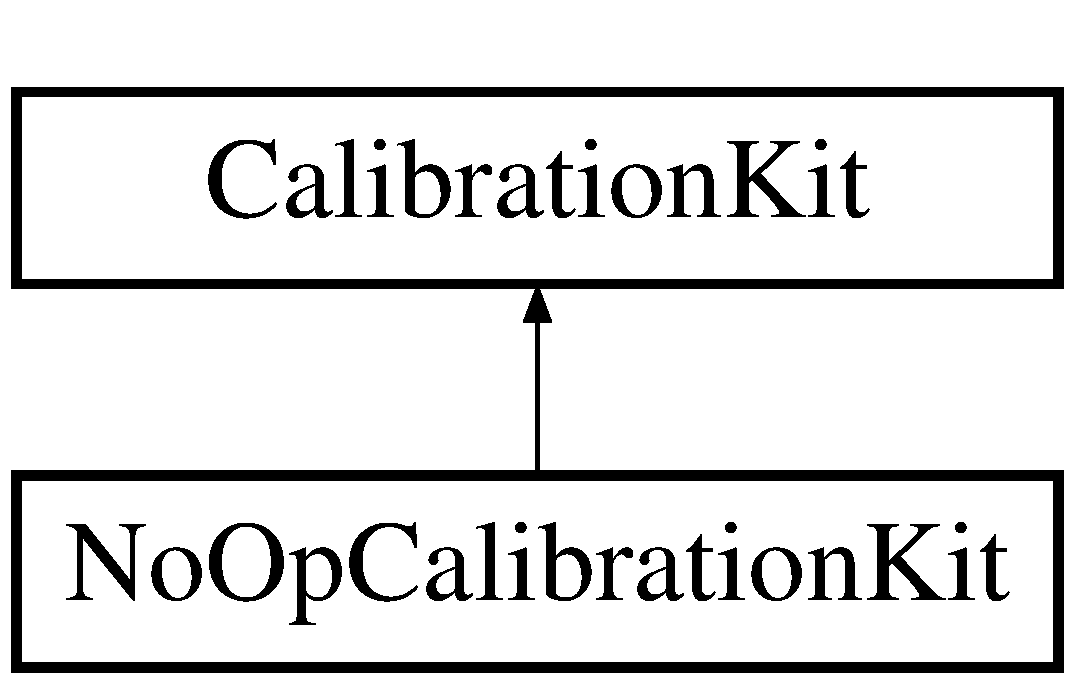
\includegraphics[height=2cm]{classNoOpCalibrationKit}
\end{center}
\end{figure}
\subsection*{Public Member Functions}
\begin{DoxyCompactItemize}
\item 
{\bf Calibration} $\ast$ {\bf create} (const std::string \&module\_\-type\_\-col\_\-name, const std::string \&module\_\-calibration\_\-col\_\-name) const 
\begin{DoxyCompactList}\small\item\em create calibration object. \item\end{DoxyCompactList}\end{DoxyCompactItemize}
\subsection*{Static Protected Attributes}
\begin{DoxyCompactItemize}
\item 
static {\bf NoOpCalibrationKit} {\bfseries \_\-\_\-instance}\label{classNoOpCalibrationKit_a5eb71ed34d9b318427d462277381a6da}

\end{DoxyCompactItemize}


\subsection{Detailed Description}
Create a calibration object which just returns the uncalibrated values. \begin{DoxySeeAlso}{See also}
\doxyref{NoOpCalibration}{p.}{classNoOpCalibration}. 
\end{DoxySeeAlso}


Definition at line 9 of file NoOpCalibration.cc.

\subsection{Member Function Documentation}
\index{NoOpCalibrationKit@{NoOpCalibrationKit}!create@{create}}
\index{create@{create}!NoOpCalibrationKit@{NoOpCalibrationKit}}
\subsubsection[{create}]{\setlength{\rightskip}{0pt plus 5cm}{\bf Calibration}$\ast$ NoOpCalibrationKit::create (const std::string \& {\em module\_\-type\_\-col\_\-name}, \/  const std::string \& {\em module\_\-calibration\_\-col\_\-name}) const\hspace{0.3cm}{\ttfamily  [inline, virtual]}}\label{classNoOpCalibrationKit_ac197f7bf5528b484d5b70e664655474b}


create calibration object. 
\begin{DoxyParams}{Parameters}
\item[{\em module\_\-type\_\-col\_\-name}]the name of the conditions data collection with the module types. \item[{\em module\_\-calibration\_\-col\_\-name}]the name of the conditions data collection which contains the calibration constants. FIXME: There should be a better method to hand parameters to \doxyref{Calibration}{p.}{classCalibration} objects. \end{DoxyParams}


Implements {\bf CalibrationKit} \doxyref{}{p.}{classCalibrationKit_ab3aea5671d91a7b6f5e839324cf45a70}.

Definition at line 20 of file NoOpCalibration.cc.

The documentation for this class was generated from the following file:\begin{DoxyCompactItemize}
\item 
NoOpCalibration.cc\end{DoxyCompactItemize}

\section{CALICE::NVector\_\-t$<$ T, dimension $>$ Class Template Reference}
\label{classCALICE_1_1NVector__t}\index{CALICE::NVector\_\-t@{CALICE::NVector\_\-t}}


Simple n-\/dimensional vector (size of the vector is defined at compile time) Provides methods to add and subtract vectors or multiply and divide by scalars.  


{\ttfamily \#include $<$NVector\_\-t.hh$>$}\subsection*{Public Member Functions}
\begin{DoxyCompactItemize}
\item 
{\bf NVector\_\-t} \& {\bf clear} ()
\begin{DoxyCompactList}\small\item\em Set all elements to zero. \item\end{DoxyCompactList}\item 
UInt\_\-t {\bf n} () const \label{classCALICE_1_1NVector__t_abdf25cc48054ab30cf01c410f8e8279a}

\begin{DoxyCompactList}\small\item\em Get the dimension of the vector. \item\end{DoxyCompactList}\item 
{\bf NVector\_\-t} \& {\bf set} (const T $\ast$array)
\begin{DoxyCompactList}\small\item\em Set the elements of the vector from the given array. \item\end{DoxyCompactList}\item 
Float\_\-t \& {\bf operator[$\,$]} (UInt\_\-t index)
\begin{DoxyCompactList}\small\item\em get the element of the given index (read and write access). \item\end{DoxyCompactList}\item 
const Float\_\-t \& {\bf operator[$\,$]} (UInt\_\-t index) const 
\begin{DoxyCompactList}\small\item\em get the element of the given index (read access only). \item\end{DoxyCompactList}\item 
{\bf NVector\_\-t} \& {\bf operator+=} (const {\bf NVector\_\-t} \&a)
\begin{DoxyCompactList}\small\item\em Add a vector having the same dimension to this vector. \item\end{DoxyCompactList}\item 
{\bf NVector\_\-t} \& {\bf operator-\/=} (const {\bf NVector\_\-t} \&a)
\begin{DoxyCompactList}\small\item\em Subtract a vector having the same dimension to this vector. \item\end{DoxyCompactList}\item 
{\bf NVector\_\-t} \& {\bf operator$\ast$=} (const float c)
\begin{DoxyCompactList}\small\item\em Multiply this vector by a scalar. \item\end{DoxyCompactList}\item 
{\bf NVector\_\-t} \& {\bf operator/=} (const float c)
\begin{DoxyCompactList}\small\item\em Divide this vector by a scalar. \item\end{DoxyCompactList}\item 
Float\_\-t $\ast$ {\bf data} ()
\begin{DoxyCompactList}\small\item\em get a pointer to the underlying array (read and write access). \item\end{DoxyCompactList}\item 
const Float\_\-t $\ast$ {\bf data} () const 
\begin{DoxyCompactList}\small\item\em get a pointer to the underlying array (read only access). \item\end{DoxyCompactList}\end{DoxyCompactItemize}
\subsection*{Private Attributes}
\begin{DoxyCompactItemize}
\item 
Float\_\-t {\bf \_\-x} [dimension]
\end{DoxyCompactItemize}
\subsection*{Friends}
\begin{DoxyCompactItemize}
\item 
{\footnotesize template$<$class \_\-T , int \_\-dimension$>$ }\\{\bf NVector\_\-t}$<$ \_\-T, \_\-dimension $>$ {\bfseries operator-\/} (const {\bf NVector\_\-t}$<$ \_\-T, \_\-dimension $>$ \&a, const {\bf NVector\_\-t}$<$ \_\-T, \_\-dimension $>$ \&b)\label{classCALICE_1_1NVector__t_a9bb733175a37a01d7321b0820b225e01}

\item 
{\footnotesize template$<$class \_\-T , int \_\-dimension$>$ }\\{\bf NVector\_\-t}$<$ \_\-T, \_\-dimension $>$ {\bfseries operator+} (const {\bf NVector\_\-t}$<$ \_\-T, \_\-dimension $>$ \&a, const {\bf NVector\_\-t}$<$ \_\-T, \_\-dimension $>$ \&b)\label{classCALICE_1_1NVector__t_a14dd538b8c1b06f539d35920059c34b1}

\item 
{\footnotesize template$<$class \_\-T , int \_\-dimension$>$ }\\{\bf NVector\_\-t}$<$ \_\-T, \_\-dimension $>$ {\bfseries operator$\ast$} (const {\bf NVector\_\-t}$<$ \_\-T, \_\-dimension $>$ \&a, float c)\label{classCALICE_1_1NVector__t_a5cda9aa2291927dd970b52164b84420e}

\item 
{\footnotesize template$<$class \_\-T , int \_\-dimension$>$ }\\{\bf NVector\_\-t}$<$ \_\-T, \_\-dimension $>$ {\bfseries operator$\ast$} (float c, const {\bf NVector\_\-t}$<$ \_\-T, \_\-dimension $>$ \&a)\label{classCALICE_1_1NVector__t_ad68632b35cc774c550e0597d1e684206}

\item 
{\footnotesize template$<$class \_\-T , int \_\-dimension$>$ }\\{\bf NVector\_\-t}$<$ \_\-T, \_\-dimension $>$ {\bfseries operator/} (const {\bf NVector\_\-t}$<$ \_\-T, \_\-dimension $>$ \&a, float c)\label{classCALICE_1_1NVector__t_a7aab12263c7a79ad9ac1757ff824edd7}

\item 
{\footnotesize template$<$class \_\-T , int \_\-dimension$>$ }\\Double\_\-t {\bfseries norm} (const {\bf NVector\_\-t}$<$ \_\-T, \_\-dimension $>$ \&a)\label{classCALICE_1_1NVector__t_a5615300e1940758aa72ccf31948e0337}

\item 
{\footnotesize template$<$class \_\-T , int \_\-dimension$>$ }\\Double\_\-t {\bfseries dot} (const {\bf NVector\_\-t}$<$ \_\-T, \_\-dimension $>$ \&a, const {\bf NVector\_\-t}$<$ \_\-T, \_\-dimension $>$ \&b)\label{classCALICE_1_1NVector__t_a0ec15ec6b90caf0a2d127acebd3ca055}

\item 
{\bf ThreeVector\_\-t} {\bfseries cross} (const {\bf ThreeVector\_\-t} \&a, const {\bf ThreeVector\_\-t} \&b)\label{classCALICE_1_1NVector__t_a4cad467a11b3438c7bc1afc3995ae2cb}

\end{DoxyCompactItemize}


\subsection{Detailed Description}
\subsubsection*{template$<$class T, int dimension$>$ class CALICE::NVector\_\-t$<$ T, dimension $>$}

Simple n-\/dimensional vector (size of the vector is defined at compile time) Provides methods to add and subtract vectors or multiply and divide by scalars. There are also functions to calculate the scalar and cross products (the latter for three dimensional vectors only). A flat array (currently floats only) can be casted to an \doxyref{NVector\_\-t}{p.}{classCALICE_1_1NVector__t}: {\ttfamily  lcio::CalorimeterHit $\ast$a\_\-hit; \doxyref{NVector\_\-t$<$Float\_\-t,3$>$}{p.}{classCALICE_1_1NVector__t} $\ast$vector=static\_\-cast$<$\doxyref{NVector\_\-t$<$Float\_\-t,3$>$}{p.}{classCALICE_1_1NVector__t} $\ast$$>$(a\_\-hit-\/$>$getPosition()); } 

Definition at line 29 of file NVector\_\-t.hh.

\subsection{Member Function Documentation}
\index{CALICE::NVector\_\-t@{CALICE::NVector\_\-t}!clear@{clear}}
\index{clear@{clear}!CALICE::NVector_t@{CALICE::NVector\_\-t}}
\subsubsection[{clear}]{\setlength{\rightskip}{0pt plus 5cm}template$<$class T, int dimension$>$ {\bf NVector\_\-t}\& {\bf CALICE::NVector\_\-t}$<$ T, dimension $>$::clear ()\hspace{0.3cm}{\ttfamily  [inline]}}\label{classCALICE_1_1NVector__t_acdcc0e98ea504c04cfc4341269969e5c}


Set all elements to zero. \begin{Desc}
\item[{\bf Todo}]: this only works for simple types like int, float, double. \end{Desc}


Definition at line 45 of file NVector\_\-t.hh.\index{CALICE::NVector\_\-t@{CALICE::NVector\_\-t}!data@{data}}
\index{data@{data}!CALICE::NVector_t@{CALICE::NVector\_\-t}}
\subsubsection[{data}]{\setlength{\rightskip}{0pt plus 5cm}template$<$class T, int dimension$>$ const Float\_\-t$\ast$ {\bf CALICE::NVector\_\-t}$<$ T, dimension $>$::data () const\hspace{0.3cm}{\ttfamily  [inline]}}\label{classCALICE_1_1NVector__t_ad523fba7620726c1d58a5b32c8b2d517}


get a pointer to the underlying array (read only access). \begin{Desc}
\item[{\bf Todo}]float ? not T ? \end{Desc}


Definition at line 142 of file NVector\_\-t.hh.\index{CALICE::NVector\_\-t@{CALICE::NVector\_\-t}!data@{data}}
\index{data@{data}!CALICE::NVector_t@{CALICE::NVector\_\-t}}
\subsubsection[{data}]{\setlength{\rightskip}{0pt plus 5cm}template$<$class T, int dimension$>$ Float\_\-t$\ast$ {\bf CALICE::NVector\_\-t}$<$ T, dimension $>$::data ()\hspace{0.3cm}{\ttfamily  [inline]}}\label{classCALICE_1_1NVector__t_a216c4f7afc34c21e101a4122e857a120}


get a pointer to the underlying array (read and write access). 

Definition at line 139 of file NVector\_\-t.hh.

Referenced by CALICE::SimpleHitSearch::searchHitsAndAdjustPedestalsAndNoise().\index{CALICE::NVector\_\-t@{CALICE::NVector\_\-t}!operator$\ast$=@{operator$\ast$=}}
\index{operator$\ast$=@{operator$\ast$=}!CALICE::NVector_t@{CALICE::NVector\_\-t}}
\subsubsection[{operator$\ast$=}]{\setlength{\rightskip}{0pt plus 5cm}template$<$class T, int dimension$>$ {\bf NVector\_\-t}\& {\bf CALICE::NVector\_\-t}$<$ T, dimension $>$::operator$\ast$= (const float {\em c})\hspace{0.3cm}{\ttfamily  [inline]}}\label{classCALICE_1_1NVector__t_af177ac27d671789ac8c8d61f257ccd4b}


Multiply this vector by a scalar. \begin{Desc}
\item[{\bf Todo}]the argument should not be a float but T ? \end{Desc}


Definition at line 125 of file NVector\_\-t.hh.\index{CALICE::NVector\_\-t@{CALICE::NVector\_\-t}!operator+=@{operator+=}}
\index{operator+=@{operator+=}!CALICE::NVector_t@{CALICE::NVector\_\-t}}
\subsubsection[{operator+=}]{\setlength{\rightskip}{0pt plus 5cm}template$<$class T, int dimension$>$ {\bf NVector\_\-t}\& {\bf CALICE::NVector\_\-t}$<$ T, dimension $>$::operator+= (const {\bf NVector\_\-t}$<$ T, dimension $>$ \& {\em a})\hspace{0.3cm}{\ttfamily  [inline]}}\label{classCALICE_1_1NVector__t_ab2f2ef8cb2e16956a24eafcfd5965b19}


Add a vector having the same dimension to this vector. FIXME: The compiler should create an error message if vectors of different dimensions are added Does this happen ? 

Definition at line 108 of file NVector\_\-t.hh.\index{CALICE::NVector\_\-t@{CALICE::NVector\_\-t}!operator-\/=@{operator-\/=}}
\index{operator-\/=@{operator-\/=}!CALICE::NVector_t@{CALICE::NVector\_\-t}}
\subsubsection[{operator-\/=}]{\setlength{\rightskip}{0pt plus 5cm}template$<$class T, int dimension$>$ {\bf NVector\_\-t}\& {\bf CALICE::NVector\_\-t}$<$ T, dimension $>$::operator-\/= (const {\bf NVector\_\-t}$<$ T, dimension $>$ \& {\em a})\hspace{0.3cm}{\ttfamily  [inline]}}\label{classCALICE_1_1NVector__t_a921fef3e1b5fe52897c80917a696614d}


Subtract a vector having the same dimension to this vector. FIXME: The compiler should create an error message if vectors of different dimensions are added Does this happen ? 

Definition at line 117 of file NVector\_\-t.hh.\index{CALICE::NVector\_\-t@{CALICE::NVector\_\-t}!operator/=@{operator/=}}
\index{operator/=@{operator/=}!CALICE::NVector_t@{CALICE::NVector\_\-t}}
\subsubsection[{operator/=}]{\setlength{\rightskip}{0pt plus 5cm}template$<$class T, int dimension$>$ {\bf NVector\_\-t}\& {\bf CALICE::NVector\_\-t}$<$ T, dimension $>$::operator/= (const float {\em c})\hspace{0.3cm}{\ttfamily  [inline]}}\label{classCALICE_1_1NVector__t_ab9758bc6c1ae323e33d25457b1f60993}


Divide this vector by a scalar. \begin{Desc}
\item[{\bf Todo}]the argument should not be a float but T ? \end{Desc}


Definition at line 133 of file NVector\_\-t.hh.\index{CALICE::NVector\_\-t@{CALICE::NVector\_\-t}!operator[]@{operator[]}}
\index{operator[]@{operator[]}!CALICE::NVector_t@{CALICE::NVector\_\-t}}
\subsubsection[{operator[]}]{\setlength{\rightskip}{0pt plus 5cm}template$<$class T, int dimension$>$ const Float\_\-t\& {\bf CALICE::NVector\_\-t}$<$ T, dimension $>$::operator[$\,$] (UInt\_\-t {\em index}) const\hspace{0.3cm}{\ttfamily  [inline]}}\label{classCALICE_1_1NVector__t_afb5ddce261165c101329cba31be6363b}


get the element of the given index (read access only). 
\begin{DoxyParams}{Parameters}
\item[{\em index}]the index of the element (0 to dimension -\/ 1). \end{DoxyParams}
\begin{DoxyReturn}{Returns}
reference to the element of the given index (read access only). When the preprocessor variable BOUNDARY\_\-CHECK is defined the validity of index is checked and an exception std::runtime\_\-error is thrown in case of violations. 
\end{DoxyReturn}


Definition at line 91 of file NVector\_\-t.hh.\index{CALICE::NVector\_\-t@{CALICE::NVector\_\-t}!operator[]@{operator[]}}
\index{operator[]@{operator[]}!CALICE::NVector_t@{CALICE::NVector\_\-t}}
\subsubsection[{operator[]}]{\setlength{\rightskip}{0pt plus 5cm}template$<$class T, int dimension$>$ Float\_\-t\& {\bf CALICE::NVector\_\-t}$<$ T, dimension $>$::operator[$\,$] (UInt\_\-t {\em index})\hspace{0.3cm}{\ttfamily  [inline]}}\label{classCALICE_1_1NVector__t_aa001e473489cb79a2be6bb0708b5f9be}


get the element of the given index (read and write access). 
\begin{DoxyParams}{Parameters}
\item[{\em index}]the index of the element (0 to dimension -\/ 1). \end{DoxyParams}
\begin{DoxyReturn}{Returns}
reference to the element of the given index (read and write access). When the preprocessor variable BOUNDARY\_\-CHECK is defined the validity of index is checked and an exception std::runtime\_\-error is thrown in case of violations. 
\end{DoxyReturn}


Definition at line 71 of file NVector\_\-t.hh.\index{CALICE::NVector\_\-t@{CALICE::NVector\_\-t}!set@{set}}
\index{set@{set}!CALICE::NVector_t@{CALICE::NVector\_\-t}}
\subsubsection[{set}]{\setlength{\rightskip}{0pt plus 5cm}template$<$class T, int dimension$>$ {\bf NVector\_\-t}\& {\bf CALICE::NVector\_\-t}$<$ T, dimension $>$::set (const T $\ast$ {\em array})\hspace{0.3cm}{\ttfamily  [inline]}}\label{classCALICE_1_1NVector__t_a72e8589546f57d77aa0368c56f1b9824}


Set the elements of the vector from the given array. It is assumed that the array contains the correct amount of elements (dimension of the vector). If the dimension of the given array is smaller than the dimension of this vector then the result will be undefined. 

Definition at line 59 of file NVector\_\-t.hh.

Referenced by CALICE::Box::minDistanceToPoints(), CALICE::MipSelect::processEvent(), and CALICE::Clusteriser::processEvent().

\subsection{Field Documentation}
\index{CALICE::NVector\_\-t@{CALICE::NVector\_\-t}!\_\-x@{\_\-x}}
\index{\_\-x@{\_\-x}!CALICE::NVector_t@{CALICE::NVector\_\-t}}
\subsubsection[{\_\-x}]{\setlength{\rightskip}{0pt plus 5cm}template$<$class T, int dimension$>$ Float\_\-t {\bf CALICE::NVector\_\-t}$<$ T, dimension $>$::{\bf \_\-x}[dimension]\hspace{0.3cm}{\ttfamily  [private]}}\label{classCALICE_1_1NVector__t_a8089ceb5c1305789d489631c1da4913c}
\begin{Desc}
\item[{\bf Todo}]float ? not T ? \end{Desc}
\begin{Desc}
\item[{\bf Todo}]float ? not T ? \end{Desc}


Definition at line 142 of file NVector\_\-t.hh.

Referenced by CALICE::NVector\_\-t$<$ Float\_\-t, 3 $>$::clear(), CALICE::NVector\_\-t$<$ Float\_\-t, 3 $>$::data(), CALICE::NVector\_\-t$<$ Float\_\-t, 3 $>$::operator$\ast$=(), CALICE::NVector\_\-t$<$ Float\_\-t, 3 $>$::operator+=(), CALICE::NVector\_\-t$<$ Float\_\-t, 3 $>$::operator-\/=(), CALICE::NVector\_\-t$<$ Float\_\-t, 3 $>$::operator/=(), CALICE::NVector\_\-t$<$ Float\_\-t, 3 $>$::operator[$\,$](), and CALICE::NVector\_\-t$<$ Float\_\-t, 3 $>$::set().

The documentation for this class was generated from the following file:\begin{DoxyCompactItemize}
\item 
NVector\_\-t.hh\end{DoxyCompactItemize}

\section{CALICE::PedestalNoiseHistograms Class Reference}
\label{classCALICE_1_1PedestalNoiseHistograms}\index{CALICE::PedestalNoiseHistograms@{CALICE::PedestalNoiseHistograms}}
Inheritance diagram for CALICE::PedestalNoiseHistograms::\begin{figure}[H]
\begin{center}
\leavevmode
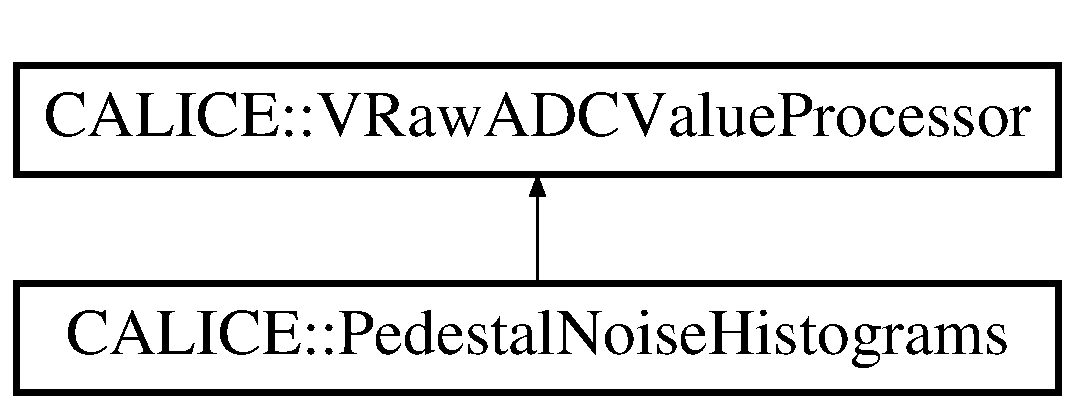
\includegraphics[height=2cm]{classCALICE_1_1PedestalNoiseHistograms}
\end{center}
\end{figure}
\subsection*{Public Member Functions}
\begin{DoxyCompactItemize}
\item 
Processor $\ast$ {\bfseries newProcessor} ()\label{classCALICE_1_1PedestalNoiseHistograms_ae5a513bca3d9c3fa642c3006723a3c40}

\item 
void {\bf init} ()
\begin{DoxyCompactList}\small\item\em Called at the begin of the job before anything is read. \item\end{DoxyCompactList}\item 
void {\bf processRunHeader} (LCRunHeader $\ast$run)
\begin{DoxyCompactList}\small\item\em Called for every run, e.g. \item\end{DoxyCompactList}\item 
void {\bf processEvent} (LCEvent $\ast$evtP)
\begin{DoxyCompactList}\small\item\em Called for every event -\/ the working horse. \item\end{DoxyCompactList}\item 
void {\bfseries end} ()\label{classCALICE_1_1PedestalNoiseHistograms_a0b92f798c4e9e32ffb7e938136db8e20}

\end{DoxyCompactItemize}
\subsection*{Protected Types}
\begin{DoxyCompactItemize}
\item 
enum {\bfseries EH1Type} \{ {\bfseries kH1Noise}, 
{\bfseries kH1Pedestal}, 
{\bfseries kNH1}
 \}
\end{DoxyCompactItemize}
\subsection*{Protected Member Functions}
\begin{DoxyCompactItemize}
\item 
void {\bfseries moduleTypeChanged} (lcio::LCCollection $\ast$col)\label{classCALICE_1_1PedestalNoiseHistograms_a2e3c07637bf5c56983d397633da2088c}

\item 
void {\bfseries moduleLocationChanged} (lcio::LCCollection $\ast$col)\label{classCALICE_1_1PedestalNoiseHistograms_a19422319fb37675b47ed8b75c751c518}

\item 
void {\bfseries moduleConnectionChanged} (lcio::LCCollection $\ast$col)\label{classCALICE_1_1PedestalNoiseHistograms_a45a6819f1ecd53413ea4c3384130f956}

\item 
void {\bfseries detectorChanged} ()\label{classCALICE_1_1PedestalNoiseHistograms_a9c381457a97f7d6a5719c106cfe22470}

\item 
void {\bfseries createHistograms} ()\label{classCALICE_1_1PedestalNoiseHistograms_a12ca8d443b6eaaaabdf30d6ab744cd77}

\end{DoxyCompactItemize}
\subsection*{Protected Attributes}
\begin{DoxyCompactItemize}
\item 
std::string {\bfseries \_\-cellParameterCollectionName}\label{classCALICE_1_1PedestalNoiseHistograms_abaadb2fa0bbd710ae117f584641b8fdb}

\item 
IntVec {\bfseries \_\-eventPar}\label{classCALICE_1_1PedestalNoiseHistograms_ae861039b81067ae12a5dea74318f8435}

\item 
{\bf histmgr::Key\_\-t} {\bfseries \_\-histogramGroupKey}\label{classCALICE_1_1PedestalNoiseHistograms_af57634693e902aa26716096d357796fe}

\item 
lcio::FloatVec {\bfseries \_\-noiseHistPar}\label{classCALICE_1_1PedestalNoiseHistograms_a5e6e5886b0245d89be77ccc0f116fecb}

\item 
lcio::FloatVec {\bfseries \_\-adcHistPar}\label{classCALICE_1_1PedestalNoiseHistograms_a79d98a735280c78211ffcb464cd1173a}

\item 
{\bf histmgr::Key\_\-t} {\bfseries \_\-histKey} [kNH1]\label{classCALICE_1_1PedestalNoiseHistograms_a24c5e21337d538e38f8f53d1219bdd91}

\item 
UInt\_\-t {\bfseries \_\-missingCellParameters}\label{classCALICE_1_1PedestalNoiseHistograms_a6e32fc4df33029b95b827bbee5700046}

\end{DoxyCompactItemize}


\subsection{Detailed Description}


Definition at line 14 of file PedestalNoiseHistograms.hh.

\subsection{Member Function Documentation}
\index{CALICE::PedestalNoiseHistograms@{CALICE::PedestalNoiseHistograms}!init@{init}}
\index{init@{init}!CALICE::PedestalNoiseHistograms@{CALICE::PedestalNoiseHistograms}}
\subsubsection[{init}]{\setlength{\rightskip}{0pt plus 5cm}void CALICE::PedestalNoiseHistograms::init ()}\label{classCALICE_1_1PedestalNoiseHistograms_a1558ef3262c57736081abced8094309e}


Called at the begin of the job before anything is read. Use to initialize the processor, e.g. book histograms. 

Reimplemented from {\bf CALICE::VRawADCValueProcessor} \doxyref{}{p.}{classCALICE_1_1VRawADCValueProcessor}.

Definition at line 76 of file PedestalNoiseHistograms.cc.

References histmgr::HistMgr::createHistogramGroup().\index{CALICE::PedestalNoiseHistograms@{CALICE::PedestalNoiseHistograms}!processEvent@{processEvent}}
\index{processEvent@{processEvent}!CALICE::PedestalNoiseHistograms@{CALICE::PedestalNoiseHistograms}}
\subsubsection[{processEvent}]{\setlength{\rightskip}{0pt plus 5cm}void CALICE::PedestalNoiseHistograms::processEvent (LCEvent $\ast$ {\em evtP})}\label{classCALICE_1_1PedestalNoiseHistograms_ac566102ce7a3f344a139d470e184dc17}


Called for every event -\/ the working horse. 

Definition at line 89 of file PedestalNoiseHistograms.cc.

References CALICE::CellParameterAccess::getCellParameter(), histmgr::HistMgr::getHistogramCollection(), CALICE::CellParameter::getNoise(), CALICE::CellParameter::getPedestal(), and histmgr::HistogramCollection\_\-t::histogram().\index{CALICE::PedestalNoiseHistograms@{CALICE::PedestalNoiseHistograms}!processRunHeader@{processRunHeader}}
\index{processRunHeader@{processRunHeader}!CALICE::PedestalNoiseHistograms@{CALICE::PedestalNoiseHistograms}}
\subsubsection[{processRunHeader}]{\setlength{\rightskip}{0pt plus 5cm}void CALICE::PedestalNoiseHistograms::processRunHeader (LCRunHeader $\ast$ {\em run})\hspace{0.3cm}{\ttfamily  [inline]}}\label{classCALICE_1_1PedestalNoiseHistograms_aabc18a7d7cd2fd0e96030c16aa4d10bd}


Called for every run, e.g. overwrite to initialize run dependent histograms. 

Definition at line 31 of file PedestalNoiseHistograms.hh.

The documentation for this class was generated from the following files:\begin{DoxyCompactItemize}
\item 
PedestalNoiseHistograms.hh\item 
PedestalNoiseHistograms.cc\end{DoxyCompactItemize}

\section{CALICE::PedestalOnTheFlyProcessor Class Reference}
\label{classCALICE_1_1PedestalOnTheFlyProcessor}\index{CALICE::PedestalOnTheFlyProcessor@{CALICE::PedestalOnTheFlyProcessor}}


Processor which calulates the pedestals from pedestal events and subtracts these values from following non-\/pedestal events.  


{\ttfamily \#include $<$PedestalOnTheFlyProcessor.hh$>$}\subsection*{Public Member Functions}
\begin{DoxyCompactItemize}
\item 
{\bf PedestalOnTheFlyProcessor} $\ast$ {\bfseries newProcessor} ()\label{classCALICE_1_1PedestalOnTheFlyProcessor_a10c562d70b7a3a6822d1d787680a1e2c}

\item 
virtual void {\bfseries init} ()\label{classCALICE_1_1PedestalOnTheFlyProcessor_a39648da7746870ad75bafa83eab06a09}

\item 
void {\bfseries processEvent} (lcio::LCEvent $\ast$evt)\label{classCALICE_1_1PedestalOnTheFlyProcessor_ab4d4773fe6ce8137a8e6e8f3b10c97c5}

\item 
virtual void {\bfseries end} ()\label{classCALICE_1_1PedestalOnTheFlyProcessor_a4150cde3c7b10d8f43bf28f676efefad}

\end{DoxyCompactItemize}
\subsection*{Protected Attributes}
\begin{DoxyCompactItemize}
\item 
std::string {\bfseries \_\-inputColName}\label{classCALICE_1_1PedestalOnTheFlyProcessor_a715f7012132a51ed82c00b9e500980aa}

\item 
std::string {\bfseries \_\-outputColName}\label{classCALICE_1_1PedestalOnTheFlyProcessor_aa4bc9785a48b64ce13a93b087b74cd67}

\item 
double {\bfseries \_\-pedSum} [HCAL\_\-N\_\-MOD+1][HCAL\_\-N\_\-CELL]\label{classCALICE_1_1PedestalOnTheFlyProcessor_a82b074fc1d3fe2bdc109b85ea8ff703e}

\item 
double {\bfseries \_\-pedSumSquare} [HCAL\_\-N\_\-MOD+1][HCAL\_\-N\_\-CELL]\label{classCALICE_1_1PedestalOnTheFlyProcessor_abde1f46084ba80f3a20c28b41398cfc1}

\item 
unsigned {\bfseries \_\-pedNum} [HCAL\_\-N\_\-MOD+1][HCAL\_\-N\_\-CELL]\label{classCALICE_1_1PedestalOnTheFlyProcessor_a3e73753bc10884fa72f30cf89c4d98d1}

\item 
float {\bfseries \_\-ped} [HCAL\_\-N\_\-MOD+1][HCAL\_\-N\_\-CELL]\label{classCALICE_1_1PedestalOnTheFlyProcessor_a40378847dcd7aff4c79795eb3fceee41}

\item 
float {\bfseries \_\-pedError} [HCAL\_\-N\_\-MOD+1][HCAL\_\-N\_\-CELL]\label{classCALICE_1_1PedestalOnTheFlyProcessor_ad4a27e50c47ca620894a12248958ddb3}

\item 
float {\bfseries \_\-significanceCut}\label{classCALICE_1_1PedestalOnTheFlyProcessor_a5776cfb8ca374fbcee4f3ca87bcf9297}

\item 
int {\bfseries \_\-skipPedestals}\label{classCALICE_1_1PedestalOnTheFlyProcessor_a3528d68a6e0a2465c8550f8da410d44b}

\item 
int {\bfseries \_\-skipStartUpPedestals}\label{classCALICE_1_1PedestalOnTheFlyProcessor_abdf7d6fec744c128abcaeb987d0ccb50}

\item 
int {\bfseries \_\-pedCounter}\label{classCALICE_1_1PedestalOnTheFlyProcessor_a33772e03ef01ae351fac171af28920ee}

\item 
int {\bfseries \_\-minPedNumber}\label{classCALICE_1_1PedestalOnTheFlyProcessor_ab104343f3071e7b73d061149f3d09262}

\item 
bool {\bfseries \_\-throwSkipEventException}\label{classCALICE_1_1PedestalOnTheFlyProcessor_a3a75fe8a1e9a744048d0c5e4e5e59092}

\end{DoxyCompactItemize}


\subsection{Detailed Description}
Processor which calulates the pedestals from pedestal events and subtracts these values from following non-\/pedestal events. \begin{DoxyAuthor}{Author}
S. Schmidt 
\end{DoxyAuthor}
\begin{DoxyDate}{Date}
Dec 2006 
\end{DoxyDate}


Definition at line 19 of file PedestalOnTheFlyProcessor.hh.

The documentation for this class was generated from the following files:\begin{DoxyCompactItemize}
\item 
PedestalOnTheFlyProcessor.hh\item 
PedestalOnTheFlyProcessor.cc\end{DoxyCompactItemize}

\section{histmgr::Profile1D Class Reference}
\label{classhistmgr_1_1Profile1D}\index{histmgr::Profile1D@{histmgr::Profile1D}}


A 1-\/dimensional histogram using float values for the bins.  


{\ttfamily \#include $<$Profile1D.hh$>$}Inheritance diagram for histmgr::Profile1D::\begin{figure}[H]
\begin{center}
\leavevmode
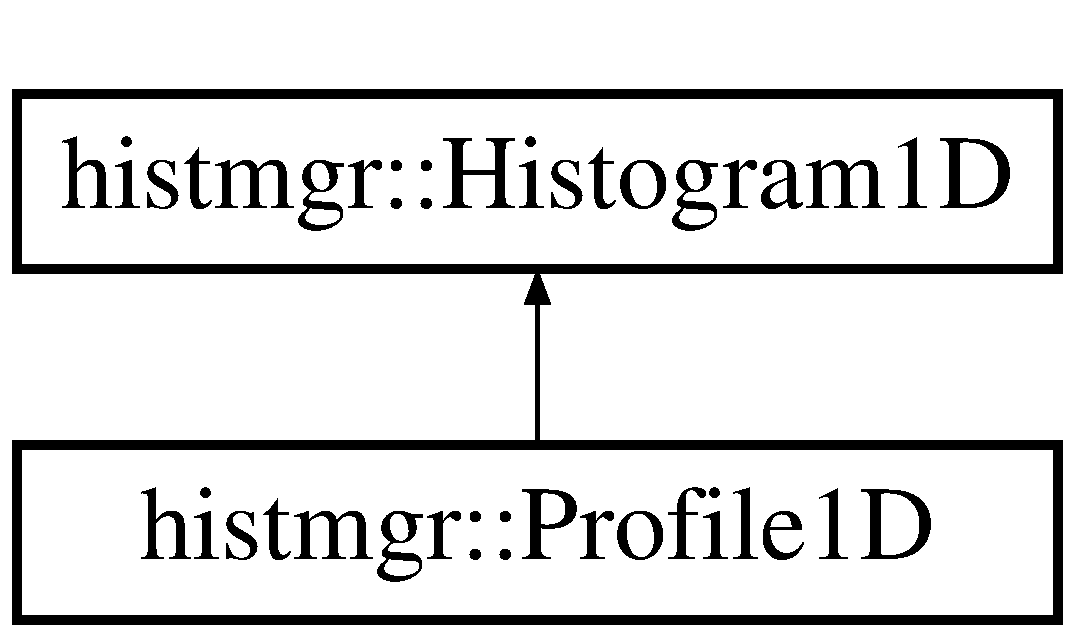
\includegraphics[height=2cm]{classhistmgr_1_1Profile1D}
\end{center}
\end{figure}
\subsection*{Public Member Functions}
\begin{DoxyCompactItemize}
\item 
{\bf Profile1D} (UInt\_\-t id, const {\bf HistPar} \&binning)
\begin{DoxyCompactList}\small\item\em Create a histogram with a certain binning. \item\end{DoxyCompactList}\item 
{\bfseries Profile1D} (lcio::LCObject $\ast$a\_\-obj)\label{classhistmgr_1_1Profile1D_a4789d7e34227713903e379a1ec7d3962}

\item 
{\bfseries Profile1D} (const {\bf Profile1D} \&a)\label{classhistmgr_1_1Profile1D_a7a6d403d74f7d436a5cbb68016580511}

\item 
void {\bf fill} (Float\_\-t x\_\-value, Double\_\-t value, Double\_\-t weight=1.)\label{classhistmgr_1_1Profile1D_a85d6672aca865b96e557323d3095b94c}

\begin{DoxyCompactList}\small\item\em fill a value into the histogram \item\end{DoxyCompactList}\item 
void {\bf reset} ()\label{classhistmgr_1_1Profile1D_a0aff38e965618142af8ecda50b721d4f}

\begin{DoxyCompactList}\small\item\em reset the histograms and the number of entries \item\end{DoxyCompactList}\item 
Double\_\-t {\bf sum} (UInt\_\-t bin\_\-index) const 
\item 
Double\_\-t {\bfseries sum2} (UInt\_\-t bin\_\-index) const \label{classhistmgr_1_1Profile1D_a27a5f854b0de6cd760a1be589a9165ef}

\item 
Double\_\-t {\bfseries mean} (UInt\_\-t bin\_\-index) const \label{classhistmgr_1_1Profile1D_a3aabceab2ad741e243aedea0bb3598d7}

\item 
Double\_\-t {\bf sigma} (UInt\_\-t bin\_\-index) const 
\begin{DoxyCompactList}\small\item\em Return the rms of the bin. \item\end{DoxyCompactList}\item 
Double\_\-t {\bfseries rms} (UInt\_\-t bin\_\-index) const \label{classhistmgr_1_1Profile1D_a25ee461c0728a5bed40dc6b020b5b220}

\item 
Double\_\-t {\bfseries min} (UInt\_\-t bin\_\-index) const \label{classhistmgr_1_1Profile1D_a5d07ca25d79482dd7d8d98178d746784}

\item 
Double\_\-t {\bfseries max} (UInt\_\-t bin\_\-index) const \label{classhistmgr_1_1Profile1D_af8406fba0e42d7c9ffcdcf66d5d193c5}

\item 
Double\_\-t {\bfseries sumOfWeights} (UInt\_\-t bin\_\-index) const \label{classhistmgr_1_1Profile1D_ac62849819ee902dffddb7aebc7536691}

\item 
void {\bfseries calculate} ()\label{classhistmgr_1_1Profile1D_ac1fc5c2662bcab8be68b5e3a5b388453}

\item 
Float\_\-t {\bfseries mean} () const \label{classhistmgr_1_1Profile1D_af5aa05e5008c1c1bae8f2c4bba9dd904}

\item 
Float\_\-t {\bf rms} () const 
\begin{DoxyCompactList}\small\item\em Root mean square as defined by ROOT. \item\end{DoxyCompactList}\item 
Float\_\-t {\bf variance} () const 
\begin{DoxyCompactList}\small\item\em Variance. \item\end{DoxyCompactList}\item 
lcio::LCObject $\ast$ {\bfseries clone} () const \label{classhistmgr_1_1Profile1D_a23277a8a779ce572ed770317146bc7ae}

\end{DoxyCompactItemize}
\subsection*{Protected Types}
\begin{DoxyCompactItemize}
\item 
enum {\bfseries EBinType} \{ \par
{\bfseries kSum}, 
{\bfseries kSum2}, 
{\bfseries kMin}, 
{\bfseries kMax}, 
\par
{\bfseries kWeightSum}, 
{\bfseries kNBinTypes}
 \}
\end{DoxyCompactItemize}
\subsection*{Protected Member Functions}
\begin{DoxyCompactItemize}
\item 
void {\bfseries addToBinContent} (UInt\_\-t type\_\-i, UInt\_\-t bin\_\-index, Double\_\-t value)\label{classhistmgr_1_1Profile1D_aadc85fd4d567c7eb28a7b4da4741ebc4}

\item 
void {\bfseries setBinContent} (UInt\_\-t type\_\-i, UInt\_\-t bin\_\-index, Double\_\-t value)\label{classhistmgr_1_1Profile1D_a7a35e0ae5777ff5f9b96c7cd19c68a23}

\item 
Double\_\-t {\bfseries binContent} (UInt\_\-t type\_\-i, UInt\_\-t bin\_\-index) const \label{classhistmgr_1_1Profile1D_a25ff38a444a39ce2105c287e0acf3955}

\item 
bool {\bfseries isCalculated} (UInt\_\-t bin\_\-index) const \label{classhistmgr_1_1Profile1D_affb2a5a6c6de2b2629ba827fff24876c}

\item 
UInt\_\-t {\bfseries getValueIndex} (UInt\_\-t type\_\-i, UInt\_\-t bin\_\-index) const \label{classhistmgr_1_1Profile1D_a27b869379f7ac5024adadf2c3a6ff848}

\end{DoxyCompactItemize}


\subsection{Detailed Description}
A 1-\/dimensional histogram using float values for the bins. 

Definition at line 13 of file Profile1D.hh.

\subsection{Constructor \& Destructor Documentation}
\index{histmgr::Profile1D@{histmgr::Profile1D}!Profile1D@{Profile1D}}
\index{Profile1D@{Profile1D}!histmgr::Profile1D@{histmgr::Profile1D}}
\subsubsection[{Profile1D}]{\setlength{\rightskip}{0pt plus 5cm}histmgr::Profile1D::Profile1D (UInt\_\-t {\em id}, \/  const {\bf HistPar} \& {\em binning})}\label{classhistmgr_1_1Profile1D_a89f879d24c7404f5ac2514baa2038a54}


Create a histogram with a certain binning. 
\begin{DoxyParams}{Parameters}
\item[{\em id}]a unique histogram ID, \item[{\em binning}]number of bins and range of the axis \end{DoxyParams}
\begin{Desc}
\item[{\bf Todo}]a name would be better than an ID but a string can not be easily stored in an LCGenericObject \end{Desc}


Definition at line 8 of file Profile1D.cc.

References HistPar::nBins(), reset(), and histmgr::Histogram1D::setBinning().

\subsection{Member Function Documentation}
\index{histmgr::Profile1D@{histmgr::Profile1D}!rms@{rms}}
\index{rms@{rms}!histmgr::Profile1D@{histmgr::Profile1D}}
\subsubsection[{rms}]{\setlength{\rightskip}{0pt plus 5cm}Float\_\-t histmgr::Profile1D::rms () const}\label{classhistmgr_1_1Profile1D_a79200e6ccc8ce76412dfcd9655319605}


Root mean square as defined by ROOT. divided by n 

Definition at line 63 of file Profile1D.cc.

References histmgr::Histogram1D::firstBinIndex(), histmgr::Histogram1D::lastBinIndex(), histmgr::Histogram1D::nBins(), sum(), histmgr::Histogram1D::xMax(), and histmgr::Histogram1D::xMin().

Referenced by sigma().\index{histmgr::Profile1D@{histmgr::Profile1D}!sigma@{sigma}}
\index{sigma@{sigma}!histmgr::Profile1D@{histmgr::Profile1D}}
\subsubsection[{sigma}]{\setlength{\rightskip}{0pt plus 5cm}Double\_\-t histmgr::Profile1D::sigma (UInt\_\-t {\em bin\_\-index}) const\hspace{0.3cm}{\ttfamily  [inline]}}\label{classhistmgr_1_1Profile1D_acfc518a1e2e4bb73ab7e696eafd1c12a}


Return the rms of the bin. deprecated. 

Definition at line 81 of file Profile1D.hh.

References rms().\index{histmgr::Profile1D@{histmgr::Profile1D}!sum@{sum}}
\index{sum@{sum}!histmgr::Profile1D@{histmgr::Profile1D}}
\subsubsection[{sum}]{\setlength{\rightskip}{0pt plus 5cm}Double\_\-t histmgr::Profile1D::sum (UInt\_\-t {\em bin\_\-index}) const\hspace{0.3cm}{\ttfamily  [inline]}}\label{classhistmgr_1_1Profile1D_a6abef8f36f84aa8580def449b7741753}
manipulate a histogram bin 

Definition at line 201 of file Profile1D.hh.

Referenced by rms(), and variance().\index{histmgr::Profile1D@{histmgr::Profile1D}!variance@{variance}}
\index{variance@{variance}!histmgr::Profile1D@{histmgr::Profile1D}}
\subsubsection[{variance}]{\setlength{\rightskip}{0pt plus 5cm}Float\_\-t histmgr::Profile1D::variance () const}\label{classhistmgr_1_1Profile1D_afb01c1ced0cf5541fd8928ab07c78e5e}


Variance. divided by n-\/1 

Definition at line 94 of file Profile1D.cc.

References histmgr::Histogram1D::firstBinIndex(), histmgr::Histogram1D::lastBinIndex(), histmgr::Histogram1D::nBins(), sum(), histmgr::Histogram1D::xMax(), and histmgr::Histogram1D::xMin().

The documentation for this class was generated from the following files:\begin{DoxyCompactItemize}
\item 
Profile1D.hh\item 
Profile1D.cc\end{DoxyCompactItemize}

\section{histmgr::ProfileCollection\_\-t Class Reference}
\label{classhistmgr_1_1ProfileCollection__t}\index{histmgr::ProfileCollection\_\-t@{histmgr::ProfileCollection\_\-t}}


One or two dimensional collection of profile histograms.  


{\ttfamily \#include $<$ProfileCollection\_\-t.hh$>$}Inheritance diagram for histmgr::ProfileCollection\_\-t::\begin{figure}[H]
\begin{center}
\leavevmode
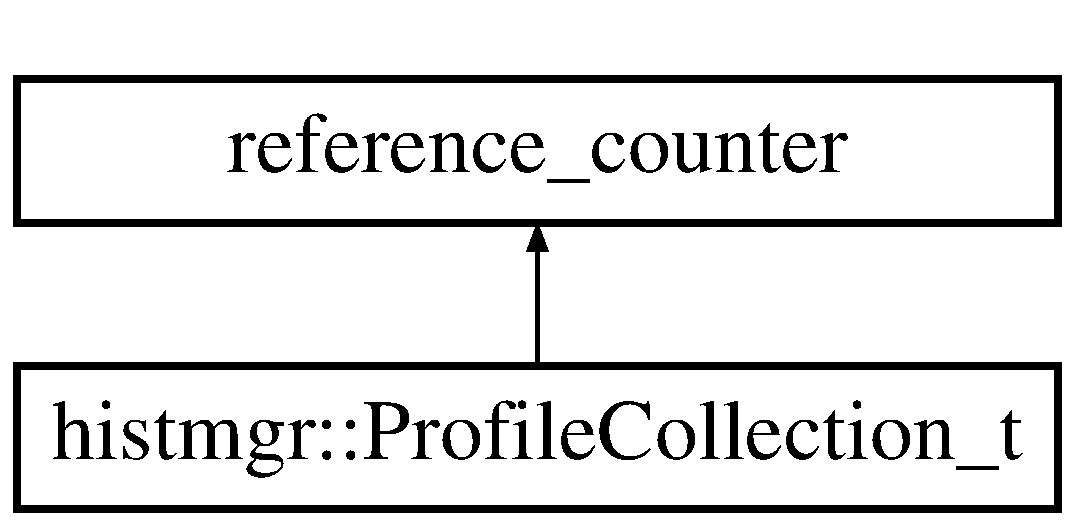
\includegraphics[height=2cm]{classhistmgr_1_1ProfileCollection__t}
\end{center}
\end{figure}
\subsection*{Public Member Functions}
\begin{DoxyCompactItemize}
\item 
{\bf ProfileCollection\_\-t} (const std::string \&collection\_\-name, const EVENT::StringVec \&name\_\-list, UInt\_\-t n\_\-hist, const {\bf HistPar} \&par)  throw (std::bad\_\-alloc, std::runtime\_\-error)
\begin{DoxyCompactList}\small\item\em Create a collection of profile histograms which will have the same binning of the x-\/axis. \item\end{DoxyCompactList}\item 
{\bf ProfileCollection\_\-t} (const std::string \&collection\_\-name, const EVENT::StringVec \&name\_\-list, const lcio::IntVec \&n\_\-hist\_\-list, const {\bf HistPar} \&par)
\begin{DoxyCompactList}\small\item\em Create a collection of profile histograms which will have the same binning of the x-\/axis. \item\end{DoxyCompactList}\item 
{\bf ProfileCollection\_\-t} (lcio::LCCollection $\ast$profile\_\-histograms, lcio::IntVec $\ast$indices)
\item 
{\bf ProfileCollection\_\-t} (lcio::LCCollection $\ast$profile\_\-histograms)
\begin{DoxyCompactList}\small\item\em Create a profile histogram collection from lcio collection. \item\end{DoxyCompactList}\item 
{\bf ProfileCollection\_\-t} (const {\bf ProfileCollection\_\-t} \&a)\label{classhistmgr_1_1ProfileCollection__t_a78705d5dbdda7837e62dad10612a3e65}

\begin{DoxyCompactList}\small\item\em copy constructor. \item\end{DoxyCompactList}\item 
{\bf ProfileCollection\_\-t} ()\label{classhistmgr_1_1ProfileCollection__t_a274f9d96d7cc79c3cb88dd089c0adeb6}

\begin{DoxyCompactList}\small\item\em Default constructor. \item\end{DoxyCompactList}\item 
void {\bf deleteCollection} ()\label{classhistmgr_1_1ProfileCollection__t_a1bcaaeb9402de2da41dfb3123a772484}

\begin{DoxyCompactList}\small\item\em delete the histogram collection and the index array This method exists instead of a destrctor to prevent copying the arrays (FIXME) \item\end{DoxyCompactList}\item 
void {\bfseries deleteSharedStorage} ()\label{classhistmgr_1_1ProfileCollection__t_a8cbe0a0888e6cdfb650eb4e8e4c8ed59}

\item 
lcio::LCCollection $\ast$ {\bf createProfiles} (const std::string \&collection\_\-name, const EVENT::StringVec \&name\_\-list, UInt\_\-t n\_\-hist, const {\bf HistPar} \&par)  throw (std::bad\_\-alloc,std::runtime\_\-error)
\begin{DoxyCompactList}\small\item\em create several histograms which will have the same binning and the same name (except of a numeric extension). \item\end{DoxyCompactList}\item 
lcio::LCCollection $\ast$ {\bf createProfiles} (const std::string \&collection\_\-name, const EVENT::StringVec \&name\_\-list, const lcio::IntVec \&n\_\-hist\_\-list, const {\bf HistPar} \&par)  throw (std::bad\_\-alloc,std::runtime\_\-error)
\begin{DoxyCompactList}\small\item\em create several histograms which will have the same binning and the same name (except of a numeric extension). \item\end{DoxyCompactList}\item 
lcio::LCCollection $\ast$ {\bf collection} ()
\begin{DoxyCompactList}\small\item\em get the unique group id \item\end{DoxyCompactList}\item 
const lcio::LCCollection $\ast$ {\bf collection} () const 
\begin{DoxyCompactList}\small\item\em get the collection of histograms (read only). \item\end{DoxyCompactList}\item 
UInt\_\-t {\bf n} () const \label{classhistmgr_1_1ProfileCollection__t_ae9944d3bd52954322ad8a7eeb9d775da}

\begin{DoxyCompactList}\small\item\em get the number of histograms in the one dimensional collection. \item\end{DoxyCompactList}\item 
bool {\bf is2D} () const \label{classhistmgr_1_1ProfileCollection__t_a60150d80ce81ba3e0a72615f1ba0e13a}

\begin{DoxyCompactList}\small\item\em Return true if the histogram collection is two instead of one diemensional. \item\end{DoxyCompactList}\item 
UInt\_\-t {\bf nMajor} () const \label{classhistmgr_1_1ProfileCollection__t_a7f7bfdba4d4196edbd68e1f543b9edc6}

\begin{DoxyCompactList}\small\item\em get the number of histograms in the one dimensional collection. \item\end{DoxyCompactList}\item 
UInt\_\-t {\bf nMinor} (UInt\_\-t major\_\-index) const \label{classhistmgr_1_1ProfileCollection__t_af49567f40d7bb80029d1edb8b0cc422c}

\begin{DoxyCompactList}\small\item\em get the number of histograms in the one dimensional collection. \item\end{DoxyCompactList}\item 
const {\bf Profile1D} $\ast$ {\bf histogram} (UInt\_\-t index) const \label{classhistmgr_1_1ProfileCollection__t_a02e73b2e13af49570048079e09bdc855}

\begin{DoxyCompactList}\small\item\em Get one histogram of the collection (read only). \item\end{DoxyCompactList}\item 
{\bf Profile1D} $\ast$ {\bf histogram} (UInt\_\-t index)\label{classhistmgr_1_1ProfileCollection__t_ab51ee868a8236003fec385b8b2460638}

\begin{DoxyCompactList}\small\item\em Get one histogram of the collection. \item\end{DoxyCompactList}\item 
{\bf Profile1D} $\ast$ {\bf histogram} (UInt\_\-t major\_\-index, UInt\_\-t minor\_\-index)\label{classhistmgr_1_1ProfileCollection__t_af48025ca8cacecbcc2566c4a709a4608}

\begin{DoxyCompactList}\small\item\em Get one histogram of the collection which is organised as a two dimensional array. \item\end{DoxyCompactList}\item 
const {\bf Profile1D} $\ast$ {\bf histogram} (UInt\_\-t major\_\-index, UInt\_\-t minor\_\-index) const \label{classhistmgr_1_1ProfileCollection__t_ada8a50d8d67e5c932035bc86ab4683f1}

\begin{DoxyCompactList}\small\item\em Get one histogram of the collection which is organised as a two dimensional array (read only). \item\end{DoxyCompactList}\item 
const std::string \& {\bf getName} (UInt\_\-t major\_\-index) const 
\begin{DoxyCompactList}\small\item\em Get the name of the specified element of the histogram collection. \item\end{DoxyCompactList}\end{DoxyCompactItemize}
\subsection*{Protected Member Functions}
\begin{DoxyCompactItemize}
\item 
UInt\_\-t {\bfseries get\_\-index} (UInt\_\-t major\_\-index, UInt\_\-t minor\_\-index) const   throw (std::range\_\-error)\label{classhistmgr_1_1ProfileCollection__t_af99cfa98fd1b76998e6a7b8d9979090a}

\end{DoxyCompactItemize}
\subsection*{Static Protected Attributes}
\begin{DoxyCompactItemize}
\item 
static const std::string {\bfseries \_\-\_\-histogramNameParameterName}\label{classhistmgr_1_1ProfileCollection__t_a7fc8b680ea20277a25bd90108bbd96f7}

\end{DoxyCompactItemize}
\subsection*{Private Member Functions}
\begin{DoxyCompactItemize}
\item 
void {\bf copyNames} () const 
\begin{DoxyCompactList}\small\item\em Copy the names from the collection to an accessible vector. \item\end{DoxyCompactList}\end{DoxyCompactItemize}
\subsection*{Private Attributes}
\begin{DoxyCompactItemize}
\item 
lcio::LCCollection $\ast$ {\bf \_\-histogramCol}\label{classhistmgr_1_1ProfileCollection__t_af0f9971e6bc0a8c1c6ea03ff80599e07}

\begin{DoxyCompactList}\small\item\em the histogram collection \item\end{DoxyCompactList}\item 
lcio::IntVec $\ast$ {\bf \_\-majorIndex}
\begin{DoxyCompactList}\small\item\em optional list of offset to form a two dimensional array out of the list. \item\end{DoxyCompactList}\item 
lcio::StringVec {\bf \_\-nameList}
\begin{DoxyCompactList}\small\item\em A vector which contains one name for all histograms of the collection or a name for each element. \item\end{DoxyCompactList}\end{DoxyCompactItemize}
\subsection*{Static Private Attributes}
\begin{DoxyCompactItemize}
\item 
static const std::string {\bfseries \_\-\_\-majorIndexParameterName}\label{classhistmgr_1_1ProfileCollection__t_a1c04bf058608dd3eda9a3d20ae0e3760}

\item 
static const std::string {\bfseries \_\-\_\-defaultProfileName}\label{classhistmgr_1_1ProfileCollection__t_aba49aeee2d76d037a3f02ad41e78f917}

\end{DoxyCompactItemize}
\subsection*{Friends}
\begin{DoxyCompactItemize}
\item 
class {\bfseries HistMgr}\label{classhistmgr_1_1ProfileCollection__t_a3cc85db784d7651390e41024125eb3a0}

\end{DoxyCompactItemize}


\subsection{Detailed Description}
One or two dimensional collection of profile histograms. 

Definition at line 19 of file ProfileCollection\_\-t.hh.

\subsection{Constructor \& Destructor Documentation}
\index{histmgr::ProfileCollection\_\-t@{histmgr::ProfileCollection\_\-t}!ProfileCollection\_\-t@{ProfileCollection\_\-t}}
\index{ProfileCollection\_\-t@{ProfileCollection\_\-t}!histmgr::ProfileCollection_t@{histmgr::ProfileCollection\_\-t}}
\subsubsection[{ProfileCollection\_\-t}]{\setlength{\rightskip}{0pt plus 5cm}histmgr::ProfileCollection\_\-t::ProfileCollection\_\-t (const std::string \& {\em collection\_\-name}, \/  const EVENT::StringVec \& {\em name\_\-list}, \/  UInt\_\-t {\em n\_\-hist}, \/  const {\bf HistPar} \& {\em par})  throw (std::bad\_\-alloc, std::runtime\_\-error)\hspace{0.3cm}{\ttfamily  [inline]}}\label{classhistmgr_1_1ProfileCollection__t_a5fb18d77200f8a0074cf33ce0ce10c51}


Create a collection of profile histograms which will have the same binning of the x-\/axis. 
\begin{DoxyParams}{Parameters}
\item[{\em collection\_\-name}]the of the histogram collection \item[{\em name\_\-list}]a vector which contains a name for each profile histogram of the collection. \item[{\em n\_\-hist}]the number of histograms to be created \item[{\em par}]the binning of the histograms\end{DoxyParams}
If the name\_\-list is empty the name of the collection is used. The name will be extended by the index in the collection.

The profile histograms are only written to a file if the histogram group, to which this histogram belongs, is assigned to a file (\doxyref{histmgr::HistMgr::assignFileName}{p.}{classhistmgr_1_1HistMgr_a20e3c96a8ba6175c8036918ca7acb1e2}). 

Definition at line 36 of file ProfileCollection\_\-t.hh.

References createProfiles().\index{histmgr::ProfileCollection\_\-t@{histmgr::ProfileCollection\_\-t}!ProfileCollection\_\-t@{ProfileCollection\_\-t}}
\index{ProfileCollection\_\-t@{ProfileCollection\_\-t}!histmgr::ProfileCollection_t@{histmgr::ProfileCollection\_\-t}}
\subsubsection[{ProfileCollection\_\-t}]{\setlength{\rightskip}{0pt plus 5cm}histmgr::ProfileCollection\_\-t::ProfileCollection\_\-t (const std::string \& {\em collection\_\-name}, \/  const EVENT::StringVec \& {\em name\_\-list}, \/  const lcio::IntVec \& {\em n\_\-hist\_\-list}, \/  const {\bf HistPar} \& {\em par})\hspace{0.3cm}{\ttfamily  [inline]}}\label{classhistmgr_1_1ProfileCollection__t_a0a8e3d1c5f2952fb50184cb2183e36ec}


Create a collection of profile histograms which will have the same binning of the x-\/axis. 
\begin{DoxyParams}{Parameters}
\item[{\em collection\_\-name}]the of the histogram collection \item[{\em name\_\-list}]a vector containing the names of the profile histograms whose length is either equals n\_\-hist or is zero. In the latter case the collection name is used for the all profile histograms. \item[{\em n\_\-hist\_\-list}]the number of profile histograms to be created \item[{\em par}]the binning of the histogram\end{DoxyParams}
\begin{DoxyReturn}{Returns}
pointer to the histogram collection
\end{DoxyReturn}
The profile histograms are only written to a file if the histogram group, to which this histogram belongs, is assigned to a file (\doxyref{histmgr::HistMgr::assignFileName}{p.}{classhistmgr_1_1HistMgr_a20e3c96a8ba6175c8036918ca7acb1e2}). 

Definition at line 60 of file ProfileCollection\_\-t.hh.

References createProfiles().\index{histmgr::ProfileCollection\_\-t@{histmgr::ProfileCollection\_\-t}!ProfileCollection\_\-t@{ProfileCollection\_\-t}}
\index{ProfileCollection\_\-t@{ProfileCollection\_\-t}!histmgr::ProfileCollection_t@{histmgr::ProfileCollection\_\-t}}
\subsubsection[{ProfileCollection\_\-t}]{\setlength{\rightskip}{0pt plus 5cm}histmgr::ProfileCollection\_\-t::ProfileCollection\_\-t (lcio::LCCollection $\ast$ {\em profile\_\-histograms}, \/  lcio::IntVec $\ast$ {\em indices})\hspace{0.3cm}{\ttfamily  [inline]}}\label{classhistmgr_1_1ProfileCollection__t_a1b67fba520831f66ac54a2aeb6bb76c6}

\begin{DoxyParams}{Parameters}
\item[{\em profile\_\-histograms}]the linearised one or two dimensional collection of profile histograms \item[{\em indices}]optional list of indicies used to give two dimensional access to the profile histogram list. for each possible index of the first dimension is needed which contains the offset in the list. The second index is added to this offset. \end{DoxyParams}


Definition at line 76 of file ProfileCollection\_\-t.hh.

References \_\-majorIndex.\index{histmgr::ProfileCollection\_\-t@{histmgr::ProfileCollection\_\-t}!ProfileCollection\_\-t@{ProfileCollection\_\-t}}
\index{ProfileCollection\_\-t@{ProfileCollection\_\-t}!histmgr::ProfileCollection_t@{histmgr::ProfileCollection\_\-t}}
\subsubsection[{ProfileCollection\_\-t}]{\setlength{\rightskip}{0pt plus 5cm}histmgr::ProfileCollection\_\-t::ProfileCollection\_\-t (lcio::LCCollection $\ast$ {\em profile\_\-histograms})\hspace{0.3cm}{\ttfamily  [inline]}}\label{classhistmgr_1_1ProfileCollection__t_a70bbff98a1dc486b0fc4e10c879e7a25}


Create a profile histogram collection from lcio collection. 
\begin{DoxyParams}{Parameters}
\item[{\em profile\_\-histograms}]the linearised one or two dimensional collection of profile histograms (two dimensional collections have the collection parameter \char`\"{}major\char`\"{}). The method does not verify whether the lcio collection really is a histogram collection. However, if the collection has the parameter \char`\"{}major\char`\"{} it creates an index vector (costly operation) assuming that it is a 2d array instead of a 1d array(i.e. collection). The unique group id remains undedfined since it is not stored in the lcio collection. \end{DoxyParams}


Definition at line 98 of file ProfileCollection\_\-t.hh.

References \_\-majorIndex.

\subsection{Member Function Documentation}
\index{histmgr::ProfileCollection\_\-t@{histmgr::ProfileCollection\_\-t}!collection@{collection}}
\index{collection@{collection}!histmgr::ProfileCollection_t@{histmgr::ProfileCollection\_\-t}}
\subsubsection[{collection}]{\setlength{\rightskip}{0pt plus 5cm}const lcio::LCCollection$\ast$ histmgr::ProfileCollection\_\-t::collection () const\hspace{0.3cm}{\ttfamily  [inline]}}\label{classhistmgr_1_1ProfileCollection__t_a9cdd96fd544692edff237a6c34053ba5}


get the collection of histograms (read only). The index array needed for the two dimensional acces is added as a parameter named \char`\"{}major\char`\"{}. 

Definition at line 195 of file ProfileCollection\_\-t.hh.

References \_\-histogramCol.\index{histmgr::ProfileCollection\_\-t@{histmgr::ProfileCollection\_\-t}!collection@{collection}}
\index{collection@{collection}!histmgr::ProfileCollection_t@{histmgr::ProfileCollection\_\-t}}
\subsubsection[{collection}]{\setlength{\rightskip}{0pt plus 5cm}lcio::LCCollection$\ast$ histmgr::ProfileCollection\_\-t::collection ()\hspace{0.3cm}{\ttfamily  [inline]}}\label{classhistmgr_1_1ProfileCollection__t_a729c27c094e3f6cae0c5792d4e5367c2}


get the unique group id get the collection of histograms. The index array needed for the two dimensional acces is added as a parameter named \char`\"{}major\char`\"{}. 

Definition at line 190 of file ProfileCollection\_\-t.hh.

References \_\-histogramCol.\index{histmgr::ProfileCollection\_\-t@{histmgr::ProfileCollection\_\-t}!copyNames@{copyNames}}
\index{copyNames@{copyNames}!histmgr::ProfileCollection_t@{histmgr::ProfileCollection\_\-t}}
\subsubsection[{copyNames}]{\setlength{\rightskip}{0pt plus 5cm}void histmgr::ProfileCollection\_\-t::copyNames () const\hspace{0.3cm}{\ttfamily  [inline, private]}}\label{classhistmgr_1_1ProfileCollection__t_a8ed4cfba171f0974428de8c3d33dc48b}


Copy the names from the collection to an accessible vector. The vector of histogram names is attached as a parameter to the LCCollection. 

Definition at line 275 of file ProfileCollection\_\-t.hh.

References \_\-histogramCol, and \_\-nameList.

Referenced by getName().\index{histmgr::ProfileCollection\_\-t@{histmgr::ProfileCollection\_\-t}!createProfiles@{createProfiles}}
\index{createProfiles@{createProfiles}!histmgr::ProfileCollection_t@{histmgr::ProfileCollection\_\-t}}
\subsubsection[{createProfiles}]{\setlength{\rightskip}{0pt plus 5cm}lcio::LCCollection $\ast$ histmgr::ProfileCollection\_\-t::createProfiles (const std::string \& {\em collection\_\-name}, \/  const EVENT::StringVec \& {\em name\_\-list}, \/  const lcio::IntVec \& {\em n\_\-hist\_\-list}, \/  const {\bf HistPar} \& {\em par})  throw (std::bad\_\-alloc,std::runtime\_\-error)}\label{classhistmgr_1_1ProfileCollection__t_ac051f19a6fc0cd8ba52792bee2c33158}


create several histograms which will have the same binning and the same name (except of a numeric extension). 
\begin{DoxyParams}{Parameters}
\item[{\em collection\_\-name}]the of the histogram collection \item[{\em name\_\-list}]a vector containing the names of the histograms whose length is either equals n\_\-hist or is zero. In the latter case the collection name is used for the all histograms. \item[{\em n\_\-hist\_\-list}]the number of histograms to be created \item[{\em par}]the binning of the histogram\end{DoxyParams}
\begin{DoxyReturn}{Returns}
pointer to the histogram collection
\end{DoxyReturn}
The histograms are only written to a file if the histogram group, to which this histogram belongs, is assigned to a file (\doxyref{histmgr::HistMgr::assignFileName}{p.}{classhistmgr_1_1HistMgr_a20e3c96a8ba6175c8036918ca7acb1e2}). 

Definition at line 66 of file ProfileCollection\_\-t.cc.\index{histmgr::ProfileCollection\_\-t@{histmgr::ProfileCollection\_\-t}!createProfiles@{createProfiles}}
\index{createProfiles@{createProfiles}!histmgr::ProfileCollection_t@{histmgr::ProfileCollection\_\-t}}
\subsubsection[{createProfiles}]{\setlength{\rightskip}{0pt plus 5cm}lcio::LCCollection $\ast$ histmgr::ProfileCollection\_\-t::createProfiles (const std::string \& {\em collection\_\-name}, \/  const EVENT::StringVec \& {\em name\_\-list}, \/  UInt\_\-t {\em n\_\-hist}, \/  const {\bf HistPar} \& {\em par})  throw (std::bad\_\-alloc,std::runtime\_\-error)}\label{classhistmgr_1_1ProfileCollection__t_ab596c78d6a64cf999f85bfa02a2e17fc}


create several histograms which will have the same binning and the same name (except of a numeric extension). 
\begin{DoxyParams}{Parameters}
\item[{\em collection\_\-name}]the of the histogram collection \item[{\em name\_\-list}]a vector containing the names of the profile histograms whose length is either equals n\_\-hist or is zero. In the latter case the collection name is used for the all profile histograms. \item[{\em n\_\-hist}]the number of histograms to be created \item[{\em par}]the binning of the histograms\end{DoxyParams}
\begin{DoxyReturn}{Returns}
pointer to the histogram collection.
\end{DoxyReturn}
The histograms are only written to a file if the histogram group, to which this histogram belongs, is assigned to a file (\doxyref{histmgr::HistMgr::assignFileName}{p.}{classhistmgr_1_1HistMgr_a20e3c96a8ba6175c8036918ca7acb1e2}). 

Definition at line 16 of file ProfileCollection\_\-t.cc.

Referenced by ProfileCollection\_\-t().\index{histmgr::ProfileCollection\_\-t@{histmgr::ProfileCollection\_\-t}!getName@{getName}}
\index{getName@{getName}!histmgr::ProfileCollection_t@{histmgr::ProfileCollection\_\-t}}
\subsubsection[{getName}]{\setlength{\rightskip}{0pt plus 5cm}const std::string\& histmgr::ProfileCollection\_\-t::getName (UInt\_\-t {\em major\_\-index}) const\hspace{0.3cm}{\ttfamily  [inline]}}\label{classhistmgr_1_1ProfileCollection__t_afcda495caee23828146923e3bc077947}


Get the name of the specified element of the histogram collection. 
\begin{DoxyParams}{Parameters}
\item[{\em major\_\-index}]the index of the histogram element or in case of an 2D histogram array the major index. \end{DoxyParams}
\begin{DoxyReturn}{Returns}
a reference to the name. 
\end{DoxyReturn}


Definition at line 259 of file ProfileCollection\_\-t.hh.

References \_\-nameList, and copyNames().

\subsection{Field Documentation}
\index{histmgr::ProfileCollection\_\-t@{histmgr::ProfileCollection\_\-t}!\_\-majorIndex@{\_\-majorIndex}}
\index{\_\-majorIndex@{\_\-majorIndex}!histmgr::ProfileCollection_t@{histmgr::ProfileCollection\_\-t}}
\subsubsection[{\_\-majorIndex}]{\setlength{\rightskip}{0pt plus 5cm}lcio::IntVec$\ast$ {\bf histmgr::ProfileCollection\_\-t::\_\-majorIndex}\hspace{0.3cm}{\ttfamily  [private]}}\label{classhistmgr_1_1ProfileCollection__t_a8d326d21db86a5dfe18d5abc8f08246c}


optional list of offset to form a two dimensional array out of the list. 

Definition at line 285 of file ProfileCollection\_\-t.hh.

Referenced by deleteCollection(), is2D(), nMajor(), nMinor(), and ProfileCollection\_\-t().\index{histmgr::ProfileCollection\_\-t@{histmgr::ProfileCollection\_\-t}!\_\-nameList@{\_\-nameList}}
\index{\_\-nameList@{\_\-nameList}!histmgr::ProfileCollection_t@{histmgr::ProfileCollection\_\-t}}
\subsubsection[{\_\-nameList}]{\setlength{\rightskip}{0pt plus 5cm}lcio::StringVec {\bf histmgr::ProfileCollection\_\-t::\_\-nameList}\hspace{0.3cm}{\ttfamily  [mutable, private]}}\label{classhistmgr_1_1ProfileCollection__t_abb30fd62e84b6a91452d455c67b62107}


A vector which contains one name for all histograms of the collection or a name for each element. 

Definition at line 287 of file ProfileCollection\_\-t.hh.

Referenced by copyNames(), and getName().

The documentation for this class was generated from the following files:\begin{DoxyCompactItemize}
\item 
ProfileCollection\_\-t.hh\item 
ProfileCollection\_\-t.cc\end{DoxyCompactItemize}

\section{CALICE::ProgressHandler Class Reference}
\label{classCALICE_1_1ProgressHandler}\index{CALICE::ProgressHandler@{CALICE::ProgressHandler}}


Show processing progess and catch SIGINT signals and abort processing safely.  


{\ttfamily \#include $<$ProgressHandler.hh$>$}\subsection*{Public Member Functions}
\begin{DoxyCompactItemize}
\item 
Processor $\ast$ {\bfseries newProcessor} ()\label{classCALICE_1_1ProgressHandler_ab9a164476b9d7ae48a62bdbf31d3d219}

\item 
void {\bfseries init} ()\label{classCALICE_1_1ProgressHandler_a054b69defd0b5ae194a05a3bbef53d9c}

\item 
void {\bfseries processRunHeader} (LCRunHeader $\ast$run)\label{classCALICE_1_1ProgressHandler_a5692dc60a5b481b81dfdb88cafd5e84e}

\item 
void {\bfseries processEvent} (LCEvent $\ast$evtP)\label{classCALICE_1_1ProgressHandler_ad9abf9d99f305ba58d64f83dbd6dfa29}

\item 
void {\bfseries end} ()\label{classCALICE_1_1ProgressHandler_a60b8c8df282bbb3901dd5dfb6f02403d}

\end{DoxyCompactItemize}
\subsection*{Static Public Member Functions}
\begin{DoxyCompactItemize}
\item 
static void {\bf setAborted} ()\label{classCALICE_1_1ProgressHandler_a5258ed9a3ad4f59da1045a0790e4cc74}

\begin{DoxyCompactList}\small\item\em This will cause the analysis to abort when done with the current event. \item\end{DoxyCompactList}\end{DoxyCompactItemize}
\subsection*{Static Protected Member Functions}
\begin{DoxyCompactItemize}
\item 
static bool {\bf isAborted} ()
\begin{DoxyCompactList}\small\item\em check if (control-\/C) was catched \item\end{DoxyCompactList}\item 
static void {\bf installSignalHandler} ()\label{classCALICE_1_1ProgressHandler_add3606096993d34657d1a4cb4e5828f9}

\begin{DoxyCompactList}\small\item\em install signal handler \item\end{DoxyCompactList}\item 
static void {\bf removeSignalHandler} ()\label{classCALICE_1_1ProgressHandler_a6f371ea8b3b47432677bdf580737d971}

\begin{DoxyCompactList}\small\item\em remove signal handler \item\end{DoxyCompactList}\item 
static void {\bf termSignalHandler} (int sig)
\begin{DoxyCompactList}\small\item\em the signal handler \item\end{DoxyCompactList}\end{DoxyCompactItemize}
\subsection*{Protected Attributes}
\begin{DoxyCompactItemize}
\item 
unsigned int {\bfseries \_\-nEvents}\label{classCALICE_1_1ProgressHandler_a9dfcf152bfc410de7061322a16e8e143}

\item 
unsigned int {\bfseries \_\-nRuns}\label{classCALICE_1_1ProgressHandler_abe779e4dea0141cfc502f334a378d30f}

\item 
unsigned int {\bfseries \_\-nEventsRun}\label{classCALICE_1_1ProgressHandler_a8b8a9805b0e8be5e71a33e1bb83dfbd7}

\item 
unsigned int {\bfseries \_\-nEventsAtLastReport}\label{classCALICE_1_1ProgressHandler_a0ebe108e87b9734df8121047510cc9f9}

\item 
int {\bfseries \_\-reportInterval}\label{classCALICE_1_1ProgressHandler_a1fb632e1526f217b10742b3349c38066}

\item 
time\_\-t {\bfseries \_\-startTime}\label{classCALICE_1_1ProgressHandler_a81d4a06c332d3507461c85c18c42feb5}

\item 
time\_\-t {\bfseries \_\-timeOfLastReport}\label{classCALICE_1_1ProgressHandler_a42583970d0c0489eba06efcd6e406067}

\item 
clock\_\-t {\bfseries \_\-clockOfLastEvent}\label{classCALICE_1_1ProgressHandler_a3e8bf463b9445ca57fa7f226f3261d40}

\item 
clock\_\-t {\bfseries \_\-clockOfLastReport}\label{classCALICE_1_1ProgressHandler_a8b5d5c8c4a3739444664d24af7c5f6c5}

\end{DoxyCompactItemize}
\subsection*{Static Protected Attributes}
\begin{DoxyCompactItemize}
\item 
static int {\bfseries \_\-\_\-abortSignalRecieved} = 0\label{classCALICE_1_1ProgressHandler_a4b61133fa96225b039b594590db90c0c}

\end{DoxyCompactItemize}
\begin{Indent}{\bf }\par
{\em \label{_amgrpd41d8cd98f00b204e9800998ecf8427e}
 }\begin{DoxyCompactItemize}
\item 
static int {\bfseries \_\-\_\-signalHandlerInstalled} = 0\label{classCALICE_1_1ProgressHandler_a8a5e1b9339c607b2fbc3e6c5072111e1}

\item 
static struct sigaction {\bfseries \_\-\_\-oldSignalHandler}\label{classCALICE_1_1ProgressHandler_a372d47760bc435e8ed6318199ac4fd7c}

\item 
static struct sigaction {\bfseries \_\-\_\-newSignalHandler}\label{classCALICE_1_1ProgressHandler_a5eec5f8fb4c6d335b7c44f8959170bb8}

\end{DoxyCompactItemize}
\end{Indent}


\subsection{Detailed Description}
Show processing progess and catch SIGINT signals and abort processing safely. Every several seconds the current run and event number is printed to the screen. If SIGINT is sent to the process (e.g. CTRL-\/C) the processEvent will throw a marlin::StopProcessingException. Thus, abort processing. After, that the Processor::end() methods of all active processors will be called. 

Definition at line 17 of file ProgressHandler.hh.

\subsection{Member Function Documentation}
\index{CALICE::ProgressHandler@{CALICE::ProgressHandler}!isAborted@{isAborted}}
\index{isAborted@{isAborted}!CALICE::ProgressHandler@{CALICE::ProgressHandler}}
\subsubsection[{isAborted}]{\setlength{\rightskip}{0pt plus 5cm}static bool CALICE::ProgressHandler::isAborted ()\hspace{0.3cm}{\ttfamily  [inline, static, protected]}}\label{classCALICE_1_1ProgressHandler_a8eaf9b91996f83d713fb738a6e088bcd}


check if (control-\/C) was catched \begin{DoxyReturn}{Returns}
true if control-\/C was catched 
\end{DoxyReturn}


Definition at line 60 of file ProgressHandler.hh.\index{CALICE::ProgressHandler@{CALICE::ProgressHandler}!termSignalHandler@{termSignalHandler}}
\index{termSignalHandler@{termSignalHandler}!CALICE::ProgressHandler@{CALICE::ProgressHandler}}
\subsubsection[{termSignalHandler}]{\setlength{\rightskip}{0pt plus 5cm}void CALICE::ProgressHandler::termSignalHandler (int {\em sig})\hspace{0.3cm}{\ttfamily  [static, protected]}}\label{classCALICE_1_1ProgressHandler_af312ee2a43b572f39c22b1668626a8d2}


the signal handler installed by \doxyref{installSignalHandler}{p.}{classCALICE_1_1ProgressHandler_add3606096993d34657d1a4cb4e5828f9} 
\begin{DoxyParams}{Parameters}
\item[\mbox{$\leftarrow$} {\em sig}]signal for which the handler got called \end{DoxyParams}


Definition at line 130 of file ProgressHandler.cc.

The documentation for this class was generated from the following files:\begin{DoxyCompactItemize}
\item 
ProgressHandler.hh\item 
ProgressHandler.cc\end{DoxyCompactItemize}

\section{reference\_\-counter Class Reference}
\label{classreference__counter}\index{reference\_\-counter@{reference\_\-counter}}
Inheritance diagram for reference\_\-counter::\begin{figure}[H]
\begin{center}
\leavevmode
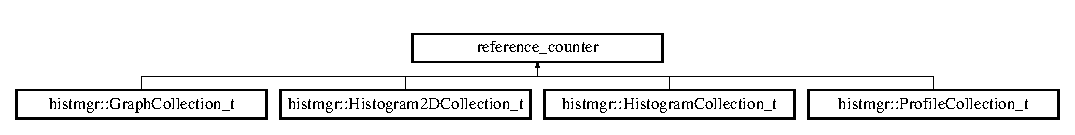
\includegraphics[height=1.37255cm]{classreference__counter}
\end{center}
\end{figure}
\subsection*{Public Member Functions}
\begin{DoxyCompactItemize}
\item 
int {\bfseries references} () const \label{classreference__counter_ac1da688951ae1a15d2b38fba6be3578e}

\item 
int {\bfseries isUsed} () const \label{classreference__counter_a150263255106bfe81c6ef086098b16bd}

\end{DoxyCompactItemize}
\subsection*{Protected Member Functions}
\begin{DoxyCompactItemize}
\item 
int {\bfseries unref} ()\label{classreference__counter_a2d715904d0723dc6daef682c98793667}

\item 
{\bf reference\_\-counter} $\ast$ {\bfseries ref} ()\label{classreference__counter_a74ffff2ab271730a149d5337db9b347d}

\end{DoxyCompactItemize}
\subsection*{Private Member Functions}
\begin{DoxyCompactItemize}
\item 
{\bf reference\_\-counter} $\ast$ {\bfseries operator\&} ()\label{classreference__counter_a8f6c78124ca5d3d6d7fd2cef42c5ad1f}

\end{DoxyCompactItemize}
\subsection*{Private Attributes}
\begin{DoxyCompactItemize}
\item 
{\bf reference\_\-counter} $\ast$ {\bfseries self}\label{classreference__counter_a8c6efecf70268743b6b1885fbe6c5db3}

\item 
int {\bfseries counter}\label{classreference__counter_a2fb8666dfcf5479be25461cbdfcbee7e}

\end{DoxyCompactItemize}
\subsection*{Friends}
\begin{DoxyCompactItemize}
\item 
class {\bf accounting\_\-ptr}\label{classreference__counter_a56b938922fd5f35053a510c4f0bd12fa}

\end{DoxyCompactItemize}


\subsection{Detailed Description}


Definition at line 10 of file reference\_\-counter.h.

The documentation for this class was generated from the following file:\begin{DoxyCompactItemize}
\item 
reference\_\-counter.h\end{DoxyCompactItemize}

\section{histmgr::RootWriter Class Reference}
\label{classhistmgr_1_1RootWriter}\index{histmgr::RootWriter@{histmgr::RootWriter}}


Write histograms to ROOT files.  


{\ttfamily \#include $<$RootWriter.hh$>$}Inheritance diagram for histmgr::RootWriter::\begin{figure}[H]
\begin{center}
\leavevmode
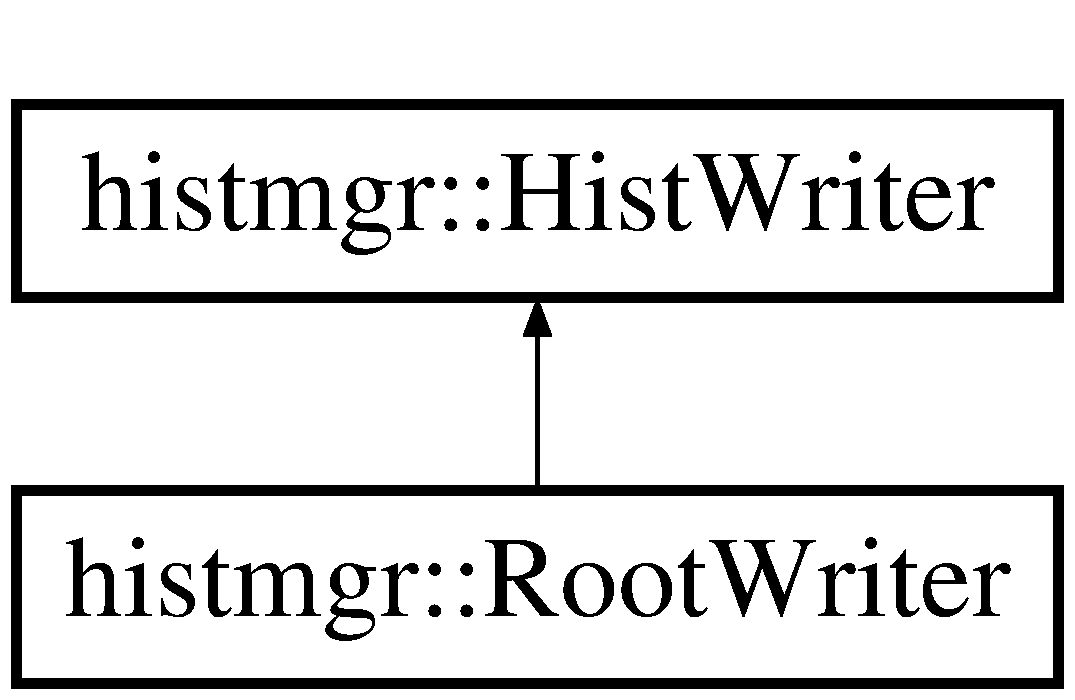
\includegraphics[height=2cm]{classhistmgr_1_1RootWriter}
\end{center}
\end{figure}
\subsection*{Public Member Functions}
\begin{DoxyCompactItemize}
\item 
{\bf RootWriter} (const std::string \&file\_\-name)
\begin{DoxyCompactList}\small\item\em create or update the given file and open for writing \item\end{DoxyCompactList}\item 
{\bf $\sim$RootWriter} ()\label{classhistmgr_1_1RootWriter_a79b1f0223f75e27831fad78194525e7b}

\begin{DoxyCompactList}\small\item\em write everything to disk, close file and destruct object. \item\end{DoxyCompactList}\item 
bool {\bf enterDir} (const std::string \&name, bool create=false)
\begin{DoxyCompactList}\small\item\em Enter a subdirectory in the file. \item\end{DoxyCompactList}\item 
void {\bf upDir} ()\label{classhistmgr_1_1RootWriter_a70902dc22a314e98cc5f6eed84bd5d7b}

\begin{DoxyCompactList}\small\item\em Go up one directory level. \item\end{DoxyCompactList}\item 
void {\bf writeToCurrentDir} (const {\bf FloatHistogram1D} \&hist, const std::string \&name)
\begin{DoxyCompactList}\small\item\em Write the given histogram to a ROOT file. \item\end{DoxyCompactList}\item 
void {\bf writeToCurrentDir} (const {\bf FloatHistogram2D} \&hist, const std::string \&name)
\begin{DoxyCompactList}\small\item\em Write the given histogram to a ROOT file. \item\end{DoxyCompactList}\item 
void {\bf writeToCurrentDir} (const EVENT::LCGenericObject $\ast$array\_\-x, const EVENT::LCGenericObject $\ast$array\_\-y, const std::string \&name)
\begin{DoxyCompactList}\small\item\em Write the given graph to a ROOT file. \item\end{DoxyCompactList}\item 
void {\bfseries writeToCurrentDir} (const EVENT::LCGenericObject $\ast$array\_\-x, const EVENT::LCGenericObject $\ast$array\_\-y, const EVENT::LCGenericObject $\ast$array\_\-ey, const std::string \&name)\label{classhistmgr_1_1RootWriter_a123cffc719468678938d9fdd127a8de0}

\end{DoxyCompactItemize}
\subsection*{Static Public Member Functions}
\begin{DoxyCompactItemize}
\item 
static TH1 $\ast$ {\bfseries createTH1} (const {\bf FloatHistogram1D} \&hist, const std::string \&name)\label{classhistmgr_1_1RootWriter_a853062957961f02909bf1e4775431fe8}

\item 
static TH2 $\ast$ {\bfseries createTH2} (const {\bf FloatHistogram2D} \&hist, const std::string \&name)\label{classhistmgr_1_1RootWriter_a8064f19b9b5d6c9f9b2f5532dc1d03d0}

\item 
static TGraph $\ast$ {\bfseries createGraph} (const EVENT::LCGenericObject $\ast$array\_\-x, const EVENT::LCGenericObject $\ast$array\_\-y, const std::string \&name)\label{classhistmgr_1_1RootWriter_ad5d2809884a4a2945b6033de0149ed90}

\item 
static TGraph $\ast$ {\bfseries createGraph} (const EVENT::LCGenericObject $\ast$array\_\-x, const EVENT::LCGenericObject $\ast$array\_\-y, const EVENT::LCGenericObject $\ast$array\_\-ey, const std::string \&name)\label{classhistmgr_1_1RootWriter_a123ada7069c614cc4044b8ab0e8c44a7}

\end{DoxyCompactItemize}
\subsection*{Static Protected Member Functions}
\begin{DoxyCompactItemize}
\item 
static TDirectory $\ast$ {\bfseries enterDir} (TDirectory $\ast$dir, const std::string \&name)\label{classhistmgr_1_1RootWriter_ae67d37f07ee5e49c049457566b6ed35a}

\end{DoxyCompactItemize}
\subsection*{Protected Attributes}
\begin{DoxyCompactItemize}
\item 
TFile $\ast$ {\bfseries \_\-file}\label{classhistmgr_1_1RootWriter_a7f36a64d91cd2fd36e58373dfef68b2e}

\item 
std::vector$<$ TDirectory $\ast$ $>$ {\bfseries \_\-dirStack}\label{classhistmgr_1_1RootWriter_ab586e486770415750374c4cb2e82b9cf}

\end{DoxyCompactItemize}


\subsection{Detailed Description}
Write histograms to ROOT files. 

Definition at line 19 of file RootWriter.hh.

\subsection{Constructor \& Destructor Documentation}
\index{histmgr::RootWriter@{histmgr::RootWriter}!RootWriter@{RootWriter}}
\index{RootWriter@{RootWriter}!histmgr::RootWriter@{histmgr::RootWriter}}
\subsubsection[{RootWriter}]{\setlength{\rightskip}{0pt plus 5cm}histmgr::RootWriter::RootWriter (const std::string \& {\em file\_\-name})}\label{classhistmgr_1_1RootWriter_a258807fed74356b5890130b3ddb1c283}


create or update the given file and open for writing 
\begin{DoxyParams}{Parameters}
\item[{\em file\_\-name}]the name including the path name of the file. \end{DoxyParams}


Definition at line 13 of file RootWriter.cc.

\subsection{Member Function Documentation}
\index{histmgr::RootWriter@{histmgr::RootWriter}!enterDir@{enterDir}}
\index{enterDir@{enterDir}!histmgr::RootWriter@{histmgr::RootWriter}}
\subsubsection[{enterDir}]{\setlength{\rightskip}{0pt plus 5cm}bool histmgr::RootWriter::enterDir (const std::string \& {\em name}, \/  bool {\em create} = {\ttfamily false})}\label{classhistmgr_1_1RootWriter_a9c162f17d8c794600eae38ec8b055a80}


Enter a subdirectory in the file. 
\begin{DoxyParams}{Parameters}
\item[{\em name}]the name of the sub directory \item[{\em create}]set to true if non existing directories shall be created \end{DoxyParams}
\begin{DoxyReturn}{Returns}
true incase the directory exists 
\end{DoxyReturn}


Definition at line 30 of file RootWriter.cc.\index{histmgr::RootWriter@{histmgr::RootWriter}!writeToCurrentDir@{writeToCurrentDir}}
\index{writeToCurrentDir@{writeToCurrentDir}!histmgr::RootWriter@{histmgr::RootWriter}}
\subsubsection[{writeToCurrentDir}]{\setlength{\rightskip}{0pt plus 5cm}void histmgr::RootWriter::writeToCurrentDir (const EVENT::LCGenericObject $\ast$ {\em array\_\-x}, \/  const EVENT::LCGenericObject $\ast$ {\em array\_\-y}, \/  const std::string \& {\em name})}\label{classhistmgr_1_1RootWriter_a23a007d670599732c86c814389e13358}


Write the given graph to a ROOT file. 
\begin{DoxyParams}{Parameters}
\item[{\em array\_\-x}]graph parameters along x \item[{\em array\_\-y}]graph parameters along y \item[{\em name}]name of the graph to be written \end{DoxyParams}
\index{histmgr::RootWriter@{histmgr::RootWriter}!writeToCurrentDir@{writeToCurrentDir}}
\index{writeToCurrentDir@{writeToCurrentDir}!histmgr::RootWriter@{histmgr::RootWriter}}
\subsubsection[{writeToCurrentDir}]{\setlength{\rightskip}{0pt plus 5cm}void histmgr::RootWriter::writeToCurrentDir (const {\bf FloatHistogram2D} \& {\em hist}, \/  const std::string \& {\em name})\hspace{0.3cm}{\ttfamily  [virtual]}}\label{classhistmgr_1_1RootWriter_a6031ddaa5a402ae73f624fb3ea2e5970}


Write the given histogram to a ROOT file. 
\begin{DoxyParams}{Parameters}
\item[{\em hist}]reference to the histogram \item[{\em name}]the name given to the histogram \end{DoxyParams}


Implements {\bf histmgr::HistWriter} \doxyref{}{p.}{classhistmgr_1_1HistWriter_a3c4e7228abcd2fe54ec6748aae6407c2}.

Definition at line 62 of file RootWriter.cc.\index{histmgr::RootWriter@{histmgr::RootWriter}!writeToCurrentDir@{writeToCurrentDir}}
\index{writeToCurrentDir@{writeToCurrentDir}!histmgr::RootWriter@{histmgr::RootWriter}}
\subsubsection[{writeToCurrentDir}]{\setlength{\rightskip}{0pt plus 5cm}void histmgr::RootWriter::writeToCurrentDir (const {\bf FloatHistogram1D} \& {\em hist}, \/  const std::string \& {\em name})\hspace{0.3cm}{\ttfamily  [virtual]}}\label{classhistmgr_1_1RootWriter_a14f07347e735118a227788b8a4c5a172}


Write the given histogram to a ROOT file. 
\begin{DoxyParams}{Parameters}
\item[{\em hist}]reference to the histogram \item[{\em name}]the name given to the histogram \end{DoxyParams}


Implements {\bf histmgr::HistWriter} \doxyref{}{p.}{classhistmgr_1_1HistWriter_ad9bdd8f2a07d67c39bb0e09e79009aa5}.

Definition at line 53 of file RootWriter.cc.

The documentation for this class was generated from the following files:\begin{DoxyCompactItemize}
\item 
RootWriter.hh\item 
RootWriter.cc\end{DoxyCompactItemize}

\section{histmgr::RootWriterKit Class Reference}
\label{classhistmgr_1_1RootWriterKit}\index{histmgr::RootWriterKit@{histmgr::RootWriterKit}}


Create a histogram writer which writes the histograms to ROOT files.  


{\ttfamily \#include $<$RootWriterKit.hh$>$}Inheritance diagram for histmgr::RootWriterKit::\begin{figure}[H]
\begin{center}
\leavevmode
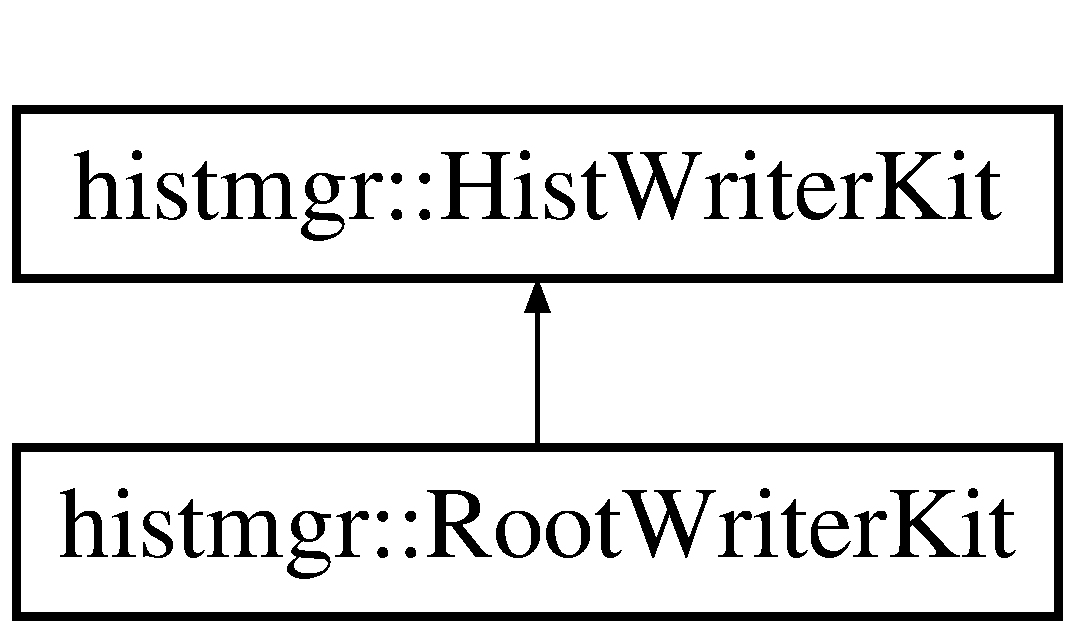
\includegraphics[height=2cm]{classhistmgr_1_1RootWriterKit}
\end{center}
\end{figure}
\subsection*{Public Member Functions}
\begin{DoxyCompactItemize}
\item 
{\bf HistWriter} $\ast$ {\bf createWriter} (const std::string \&name)
\begin{DoxyCompactList}\small\item\em create a histogram write. \item\end{DoxyCompactList}\end{DoxyCompactItemize}
\subsection*{Static Public Attributes}
\begin{DoxyCompactItemize}
\item 
static {\bf RootWriterKit} $\ast$ {\bfseries \_\-\_\-instance} = new {\bf RootWriterKit}\label{classhistmgr_1_1RootWriterKit_a6bdad8f648703ed985ec28286a58b6ee}

\end{DoxyCompactItemize}


\subsection{Detailed Description}
Create a histogram writer which writes the histograms to ROOT files. \begin{DoxySeeAlso}{See also}
\doxyref{RootWriter}{p.}{classhistmgr_1_1RootWriter}. 
\end{DoxySeeAlso}


Definition at line 12 of file RootWriterKit.hh.

\subsection{Member Function Documentation}
\index{histmgr::RootWriterKit@{histmgr::RootWriterKit}!createWriter@{createWriter}}
\index{createWriter@{createWriter}!histmgr::RootWriterKit@{histmgr::RootWriterKit}}
\subsubsection[{createWriter}]{\setlength{\rightskip}{0pt plus 5cm}{\bf HistWriter}$\ast$ histmgr::RootWriterKit::createWriter (const std::string \& {\em name})\hspace{0.3cm}{\ttfamily  [inline, virtual]}}\label{classhistmgr_1_1RootWriterKit_a480fb8728c4592098a59344922a58c71}


create a histogram write. 
\begin{DoxyParams}{Parameters}
\item[{\em name}]the name of the file to which the histograms should be written \end{DoxyParams}
\begin{DoxyReturn}{Returns}
a pointer a histogram writer which should be ready to write histograms. 
\end{DoxyReturn}


Implements {\bf histmgr::HistWriterKit} \doxyref{}{p.}{classhistmgr_1_1HistWriterKit_a4e07d5baf676d4af138d09f2e92b4001}.

Definition at line 17 of file RootWriterKit.hh.

The documentation for this class was generated from the following files:\begin{DoxyCompactItemize}
\item 
RootWriterKit.hh\item 
RootWriterKit.cc\end{DoxyCompactItemize}

\section{marlin::RunInfoProcessor Class Reference}
\label{classmarlin_1_1RunInfoProcessor}\index{marlin::RunInfoProcessor@{marlin::RunInfoProcessor}}


Preprocessor which is supposed to run at the !very! beginning of the processor chain.  


{\ttfamily \#include $<$RunInfoProcessor.hh$>$}\subsection*{Data Structures}
\begin{DoxyCompactItemize}
\item 
class {\bf LCRunModifier}
\begin{DoxyCompactList}\small\item\em Helper class to for the modification of the Run Header. \item\end{DoxyCompactList}\end{DoxyCompactItemize}
\subsection*{Public Member Functions}
\begin{DoxyCompactItemize}
\item 
virtual Processor $\ast$ {\bfseries newProcessor} ()\label{classmarlin_1_1RunInfoProcessor_ab8aa029e7fee27866206787f322b3616}

\item 
virtual void {\bf init} ()
\begin{DoxyCompactList}\small\item\em Called at the begin of the job before anything is read. \item\end{DoxyCompactList}\item 
virtual void {\bf processRunHeader} (LCRunHeader $\ast$run)\label{classmarlin_1_1RunInfoProcessor_a037d6642c5effd5ea57ef2d3dec2ce47}

\begin{DoxyCompactList}\small\item\em Called for every run. \item\end{DoxyCompactList}\item 
virtual void {\bf processEvent} (LCEvent $\ast$evt)\label{classmarlin_1_1RunInfoProcessor_a44b26122c6d673c48d5c2e0dfc5a10fd}

\begin{DoxyCompactList}\small\item\em Called for every event -\/ the working horse. \item\end{DoxyCompactList}\item 
virtual const std::string \& {\bf name} () const \label{classmarlin_1_1RunInfoProcessor_a4e0b06142a6fe83a607f8fbbfc5f3a07}

\begin{DoxyCompactList}\small\item\em Needed for modifyEvent. \item\end{DoxyCompactList}\item 
virtual void {\bfseries modifyEvent} (LCEvent $\ast$evt)\label{classmarlin_1_1RunInfoProcessor_a87835b19afc2566d1edf358c49060243}

\item 
virtual void {\bfseries check} (LCEvent $\ast$evt)\label{classmarlin_1_1RunInfoProcessor_a13101be4c139383d19a2578cac39fc21}

\item 
virtual void {\bf end} ()\label{classmarlin_1_1RunInfoProcessor_a8c82fcf3504ddc1d1cd83bd3df48b8a1}

\begin{DoxyCompactList}\small\item\em Called after data processing for clean up. \item\end{DoxyCompactList}\item 
void {\bf printRunParameters} (const LCRunHeader $\ast$run)\label{classmarlin_1_1RunInfoProcessor_ae0df13a558cff819a125d7da430d3ca8}

\begin{DoxyCompactList}\small\item\em Method to write the histograms in a ROOT file. \item\end{DoxyCompactList}\end{DoxyCompactItemize}
\subsection*{Private Member Functions}
\begin{DoxyCompactItemize}
\item 
void {\bf setVersString} (std::string)\label{classmarlin_1_1RunInfoProcessor_ac7333b2dd94c0dfaf019efda7d51783c}

\begin{DoxyCompactList}\small\item\em The function which sets the version string. \item\end{DoxyCompactList}\item 
unsigned int {\bf handleBeamParameters} (LCCDTimeStamp)
\begin{DoxyCompactList}\small\item\em Handling of beam parameters to extract energy. \item\end{DoxyCompactList}\item 
float {\bf timeCor} ()
\begin{DoxyCompactList}\small\item\em A helper function which determines corrections to be applied when check for r/o time of (cern) database of cern beam parameters. \item\end{DoxyCompactList}\item 
unsigned int {\bf getBeamEnergy} (const LCCDTimeStamp)\label{classmarlin_1_1RunInfoProcessor_af25973c2f75e0cc7d1a2e963ae6f1ae0}

\begin{DoxyCompactList}\small\item\em Method to get the beam energy from the database for a given time stamp (default). \item\end{DoxyCompactList}\item 
unsigned int {\bf getBeamEnergyUser} (const LCCDTimeStamp)\label{classmarlin_1_1RunInfoProcessor_a2a9f3d4420e6d5413b52aa4a9f909ab2}

\begin{DoxyCompactList}\small\item\em Method to get the beam energy from the database for a given time stamp (user defined settings). \item\end{DoxyCompactList}\end{DoxyCompactItemize}
\subsection*{Private Attributes}
\begin{DoxyCompactItemize}
\item 
std::string {\bf \_\-dbInit}\label{classmarlin_1_1RunInfoProcessor_a65053a1bdf8789ad7285a32739a69807}

\begin{DoxyCompactList}\small\item\em dbinit string, note that in this Processor we cannot make use of the ConditionsDataProcessor Mechanism as it may run also on MC where the event time has to be set by this processor \item\end{DoxyCompactList}\item 
std::string {\bf \_\-folderRunTime}\label{classmarlin_1_1RunInfoProcessor_aeb0c70371d7b4e0cd37581188894103e}

\begin{DoxyCompactList}\small\item\em The variable holding the folder name from which we fetch the runinfo. \item\end{DoxyCompactList}\item 
std::string {\bf \_\-folderBeamParameter}\label{classmarlin_1_1RunInfoProcessor_adbdb31a2fc1c90aa15700d0906a15b15}

\begin{DoxyCompactList}\small\item\em The folder which holds the information on the beam parameter. \item\end{DoxyCompactList}\item 
float {\bf \_\-currentTolerance}\label{classmarlin_1_1RunInfoProcessor_aab826ec0a4e9dde1f2b2d4e9a079ee22}

\begin{DoxyCompactList}\small\item\em Tolerance in \% allowed until current reading at run begin and run end is considered to be inconsinstent. \item\end{DoxyCompactList}\item 
float {\bf \_\-timeTolerance}\label{classmarlin_1_1RunInfoProcessor_abdd63cb1e6b5a847089182c30929ccb8}

\begin{DoxyCompactList}\small\item\em Tolerance in s allowed until reading of beam parameters is considered to be outdated. \item\end{DoxyCompactList}\item 
std::string {\bf \_\-folderBeamParameterException}
\begin{DoxyCompactList}\small\item\em The variable which holds the folder name for the BeamParameterException, i.e. \item\end{DoxyCompactList}\item 
std::string {\bf \_\-folderLocation}\label{classmarlin_1_1RunInfoProcessor_a1570d9cda3d532a23820e09b9da4210d}

\begin{DoxyCompactList}\small\item\em The variable which holds the name of the folder to look up the run location. \item\end{DoxyCompactList}\item 
RunLocationWhizard $\ast$ {\bf \_\-runlocationwhizard}\label{classmarlin_1_1RunInfoProcessor_a04731b4d9bb5e6635449ae5e997ea54e}

\begin{DoxyCompactList}\small\item\em The object which holds the information on the run location. \item\end{DoxyCompactList}\item 
std::string {\bf \_\-vers\_\-string}\label{classmarlin_1_1RunInfoProcessor_a281b035be172c5f29b4406256e6ff660}

\begin{DoxyCompactList}\small\item\em A string which contains the version of the converter and therefore of the db entry. \item\end{DoxyCompactList}\item 
int {\bf \_\-vers\_\-length}\label{classmarlin_1_1RunInfoProcessor_ab39f8a9b1988e14a2aeb1879d2ff2eab}

\begin{DoxyCompactList}\small\item\em The length of the version string. \item\end{DoxyCompactList}\item 
int {\bf \_\-runNumber}\label{classmarlin_1_1RunInfoProcessor_ac765ef550fc7ae185901ab1766afd0f8}

\begin{DoxyCompactList}\small\item\em Obvious variables. \item\end{DoxyCompactList}\item 
unsigned int {\bfseries \_\-beamEnergy}\label{classmarlin_1_1RunInfoProcessor_a06b6da5104e1817215b1588452dd1dd8}

\item 
int {\bf \_\-bendingCurrentToCheck}\label{classmarlin_1_1RunInfoProcessor_ad17af4643c8798dab2642df821a87952}

\begin{DoxyCompactList}\small\item\em variables needed to convert current to energy \item\end{DoxyCompactList}\item 
float {\bfseries \_\-currentToEnergy}\label{classmarlin_1_1RunInfoProcessor_aec2e8768e37e8807479bec91314b7742}

\item 
float {\bfseries \_\-toMeV}\label{classmarlin_1_1RunInfoProcessor_abbcb57bbb8ed02b4cfd48e81e5792d60}

\item 
int {\bf \_\-safetyMargin}\label{classmarlin_1_1RunInfoProcessor_aaf0d50434eb4366d31750a485d105294}

\begin{DoxyCompactList}\small\item\em Variable which can be used to ensure validity of conditions data in case of MC. \item\end{DoxyCompactList}\item 
int {\bf \_\-nRun}\label{classmarlin_1_1RunInfoProcessor_a424bd272282d83451deec7a1b3ed65d6}

\begin{DoxyCompactList}\small\item\em Obvious counter variables, needed? \item\end{DoxyCompactList}\item 
int {\bfseries \_\-nEvt}\label{classmarlin_1_1RunInfoProcessor_abfcb80607e137bb4cac4a50cb0704a07}

\item 
RunInformation $\ast$ {\bf \_\-runInformation}\label{classmarlin_1_1RunInfoProcessor_ac4fc44266d6145b8190937b9cce47c8e}

\begin{DoxyCompactList}\small\item\em An object which assembles run information. \item\end{DoxyCompactList}\item 
UTIL::LCTime {\bf \_\-eventTime}\label{classmarlin_1_1RunInfoProcessor_a892d2aa27765a45ee078d8bc713aa88f}

\begin{DoxyCompactList}\small\item\em The event time, created for MC, not in use for real data. \item\end{DoxyCompactList}\item 
bool {\bfseries \_\-overwriteRunNumber}\label{classmarlin_1_1RunInfoProcessor_ad5d607ab4fe985cfad5e419a4ea513a8}

\end{DoxyCompactItemize}


\subsection{Detailed Description}
Preprocessor which is supposed to run at the !very! beginning of the processor chain. Adding information to the Run and EventHeader, for data and MC. In partcular the beam energy is extracted from the database for a given run and the MC events get assigned a timestamp. \begin{DoxyAuthor}{Author}
: A.M. Magnan Imperial College, modifs R.Poeschl LAL
\end{DoxyAuthor}
\begin{DoxyDate}{Date}
Apr 2007 
\end{DoxyDate}
\begin{Desc}
\item[{\bf Todo}]reduce even more the dependency on hardcoded, god given parameters in the code (valid for many processors)\end{Desc}


Definition at line 52 of file RunInfoProcessor.hh.

\subsection{Member Function Documentation}
\index{marlin::RunInfoProcessor@{marlin::RunInfoProcessor}!handleBeamParameters@{handleBeamParameters}}
\index{handleBeamParameters@{handleBeamParameters}!marlin::RunInfoProcessor@{marlin::RunInfoProcessor}}
\subsubsection[{handleBeamParameters}]{\setlength{\rightskip}{0pt plus 5cm}unsigned int marlin::RunInfoProcessor::handleBeamParameters (LCCDTimeStamp {\em starttime})\hspace{0.3cm}{\ttfamily  [private]}}\label{classmarlin_1_1RunInfoProcessor_a6f3f736a349f45536e3fc13344536950}


Handling of beam parameters to extract energy. \begin{Desc}
\item[{\bf Todo}]extend scope of function and maybe turn into dedicated class \end{Desc}


Definition at line 429 of file RunInfoProcessor.cc.

References \_\-bendingCurrentToCheck, \_\-currentTolerance, \_\-dbInit, \_\-folderBeamParameter, \_\-folderBeamParameterException, \_\-runNumber, \_\-timeTolerance, and timeCor().

Referenced by getBeamEnergy().\index{marlin::RunInfoProcessor@{marlin::RunInfoProcessor}!init@{init}}
\index{init@{init}!marlin::RunInfoProcessor@{marlin::RunInfoProcessor}}
\subsubsection[{init}]{\setlength{\rightskip}{0pt plus 5cm}void marlin::RunInfoProcessor::init ()\hspace{0.3cm}{\ttfamily  [virtual]}}\label{classmarlin_1_1RunInfoProcessor_a51fa73bd662dbffa2d89a04fdd2e92da}


Called at the begin of the job before anything is read. Use to initialize the processor, e.g. book histograms. 

Definition at line 153 of file RunInfoProcessor.cc.

References \_\-nRun.\index{marlin::RunInfoProcessor@{marlin::RunInfoProcessor}!timeCor@{timeCor}}
\index{timeCor@{timeCor}!marlin::RunInfoProcessor@{marlin::RunInfoProcessor}}
\subsubsection[{timeCor}]{\setlength{\rightskip}{0pt plus 5cm}float marlin::RunInfoProcessor::timeCor ()\hspace{0.3cm}{\ttfamily  [private]}}\label{classmarlin_1_1RunInfoProcessor_a0070ee9315271f15a55ae80c4bb50acc}


A helper function which determines corrections to be applied when check for r/o time of (cern) database of cern beam parameters. \begin{Desc}
\item[{\bf Todo}]remove hardcoded times \end{Desc}


Definition at line 570 of file RunInfoProcessor.cc.

References \_\-runInformation.

Referenced by handleBeamParameters().

\subsection{Field Documentation}
\index{marlin::RunInfoProcessor@{marlin::RunInfoProcessor}!\_\-folderBeamParameterException@{\_\-folderBeamParameterException}}
\index{\_\-folderBeamParameterException@{\_\-folderBeamParameterException}!marlin::RunInfoProcessor@{marlin::RunInfoProcessor}}
\subsubsection[{\_\-folderBeamParameterException}]{\setlength{\rightskip}{0pt plus 5cm}std::string {\bf marlin::RunInfoProcessor::\_\-folderBeamParameterException}\hspace{0.3cm}{\ttfamily  [private]}}\label{classmarlin_1_1RunInfoProcessor_a36e4d01591a54d222092bd583b231f56}


The variable which holds the folder name for the BeamParameterException, i.e. to be queried in case of pbs. with automatic r/o of beam parameters. 

Definition at line 108 of file RunInfoProcessor.hh.

Referenced by getBeamEnergy(), and handleBeamParameters().

The documentation for this class was generated from the following files:\begin{DoxyCompactItemize}
\item 
RunInfoProcessor.hh\item 
RunInfoProcessor.cc\end{DoxyCompactItemize}

\section{CALICE::ScECALMappingProcessor Class Reference}
\label{classCALICE_1_1ScECALMappingProcessor}\index{CALICE::ScECALMappingProcessor@{CALICE::ScECALMappingProcessor}}


A class which converts ADCColl to CalorimeterHits with mapping change Copied and modified from \doxyref{fastMappingIIProcessor}{p.}{classCALICE_1_1fastMappingIIProcessor} Satoru Uozumi.  


{\ttfamily \#include $<$ScECALMappingProcessor.hh$>$}\subsection*{Public Member Functions}
\begin{DoxyCompactItemize}
\item 
virtual Processor $\ast$ {\bfseries newProcessor} ()\label{classCALICE_1_1ScECALMappingProcessor_aa5b4adc79f73832a1cd3bec1dbca3195}

\item 
virtual void {\bfseries conditionsChanged} (LCCollection $\ast$col)\label{classCALICE_1_1ScECALMappingProcessor_a6b292729ea8e95d8e7205b78d4275341}

\item 
virtual void {\bfseries init} ()\label{classCALICE_1_1ScECALMappingProcessor_a1e61afb80b2e210042e0771158b4df01}

\item 
virtual void {\bfseries processRunHeader} (LCRunHeader $\ast$run)\label{classCALICE_1_1ScECALMappingProcessor_a33aaaa7705715939c77d50e7186c27fe}

\item 
virtual void {\bfseries processEvent} (LCEvent $\ast$evt)\label{classCALICE_1_1ScECALMappingProcessor_adc4ca95b8fbc768edf6304d657ecda42}

\item 
virtual void {\bfseries check} (LCEvent $\ast$evt)\label{classCALICE_1_1ScECALMappingProcessor_afd9f32d4bf080574d6c4fcdcf8d3a09e}

\item 
virtual void {\bfseries end} ()\label{classCALICE_1_1ScECALMappingProcessor_a85f7c30babd95235b54d9e4a9f707451}

\end{DoxyCompactItemize}
\subsection*{Protected Member Functions}
\begin{DoxyCompactItemize}
\item 
std::pair$<$ int, int $>$ {\bfseries getScECALChannelID} (int slot, int fe, int chip, int chan)\label{classCALICE_1_1ScECALMappingProcessor_a3a07ca0b030309ec61270c833df815c8}

\item 
{\bf ThreeVector\_\-t} {\bfseries getChannelPosition} (int layer, int strip)\label{classCALICE_1_1ScECALMappingProcessor_a66a91d0d6264634c48993fa8a4db4fcd}

\end{DoxyCompactItemize}
\subsection*{Protected Attributes}
\begin{DoxyCompactItemize}
\item 
std::string {\bfseries \_\-ScECALMappingColName}\label{classCALICE_1_1ScECALMappingProcessor_ab89f9ded31a25bed66874c93731073eb}

\item 
LCCollection $\ast$ {\bfseries \_\-ScECALMappingCol}\label{classCALICE_1_1ScECALMappingProcessor_a996e63095b6c93e9a4b3927a5d0f0de8}

\item 
bool {\bfseries \_\-MappingChanged}\label{classCALICE_1_1ScECALMappingProcessor_a4a3be9d3b632b7948eac5969eea2f234}

\item 
std::string {\bfseries \_\-mappingData}\label{classCALICE_1_1ScECALMappingProcessor_a51c51a8668cb86ed04e3ca132fd5b671}

\item 
std::string {\bfseries \_\-inputColName}\label{classCALICE_1_1ScECALMappingProcessor_ab9b8252616d8e15930dd46736c0961e7}

\item 
std::string {\bfseries \_\-outputColName}\label{classCALICE_1_1ScECALMappingProcessor_a6586adf6dee846329fbeb9f68615542b}

\item 
std::pair$<$ int, int $>$ {\bfseries \_\-ScECALmap} [ScECAL\_\-NSLOT][ScECAL\_\-NFE][ScECAL\_\-NCHIP][ScECAL\_\-NCHAN]\label{classCALICE_1_1ScECALMappingProcessor_aeca6d12726f390ac358a014adf2d78f8}

\end{DoxyCompactItemize}


\subsection{Detailed Description}
A class which converts ADCColl to CalorimeterHits with mapping change Copied and modified from \doxyref{fastMappingIIProcessor}{p.}{classCALICE_1_1fastMappingIIProcessor} Satoru Uozumi. \begin{DoxyDate}{Date}
Nov 5 2008 
\end{DoxyDate}


Definition at line 39 of file ScECALMappingProcessor.hh.

The documentation for this class was generated from the following files:\begin{DoxyCompactItemize}
\item 
ScECALMappingProcessor.hh\item 
ScECALMappingProcessor.cc\end{DoxyCompactItemize}

\section{TBTrack::SimConstants Class Reference}
\label{classTBTrack_1_1SimConstants}\index{TBTrack::SimConstants@{TBTrack::SimConstants}}
Inheritance diagram for TBTrack::SimConstants::\begin{figure}[H]
\begin{center}
\leavevmode
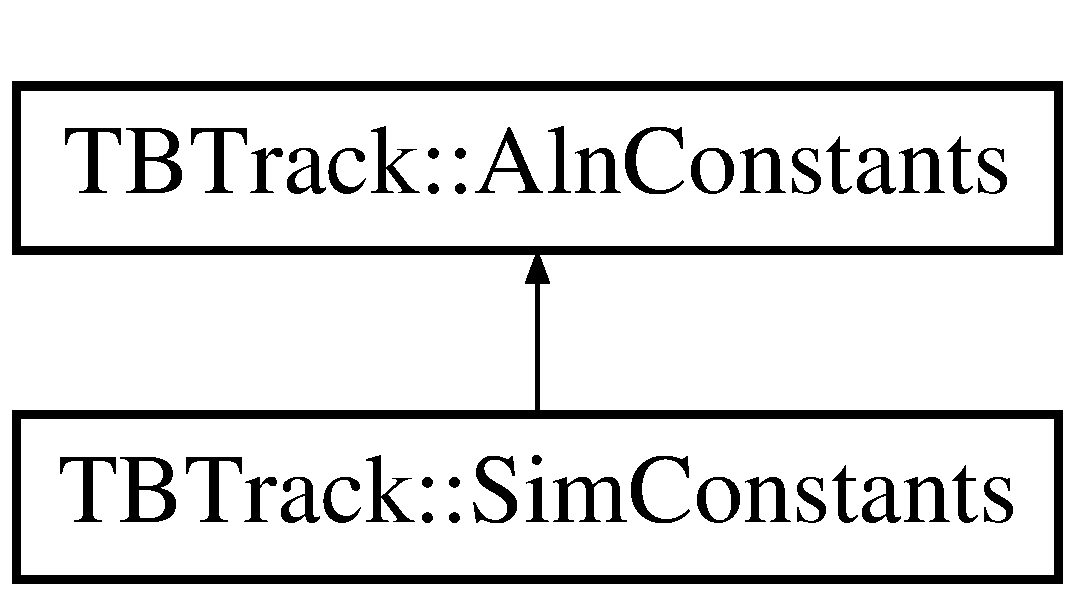
\includegraphics[height=2cm]{classTBTrack_1_1SimConstants}
\end{center}
\end{figure}
\subsection*{Public Types}
\begin{DoxyCompactItemize}
\item 
enum \{ {\bfseries numberOfInts} = 1
 \}
\item 
enum \{ {\bfseries numberOfFloats} = 0
 \}
\item 
enum \{ {\bfseries numberOfDoubles} = 4$\ast$2$\ast$4 + AlnConstants::numberOfDoubles
 \}
\end{DoxyCompactItemize}
\subsection*{Public Member Functions}
\begin{DoxyCompactItemize}
\item 
{\bfseries SimConstants} (int p=0)\label{classTBTrack_1_1SimConstants_ac985b42953f6a9db670ac9ebe4491dd3}

\item 
double {\bfseries cEffic} (unsigned d, unsigned l) const \label{classTBTrack_1_1SimConstants_a95b2a640d1fdf43d0e138df1c59097da}

\item 
void {\bfseries cEffic} (unsigned d, unsigned l, double e)\label{classTBTrack_1_1SimConstants_a57422e75c11ad31c3f76d5ed5357685f}

\item 
double {\bfseries cSmear} (unsigned d, unsigned l) const \label{classTBTrack_1_1SimConstants_a5ad8399a9a26ae1a2c8a143a0e34b54d}

\item 
void {\bfseries cSmear} (unsigned d, unsigned l, double s)\label{classTBTrack_1_1SimConstants_aef787d85563deecf9fcaf23130e1e6af}

\item 
double {\bfseries cNoise} (unsigned d, unsigned l) const \label{classTBTrack_1_1SimConstants_a05135b1be10f15e90b164c2aabd8ae1b}

\item 
void {\bfseries cNoise} (unsigned d, unsigned l, double n)\label{classTBTrack_1_1SimConstants_a206034df73ce2b627ca441e078abe2da}

\item 
double {\bfseries tTzero} (unsigned d, unsigned l) const \label{classTBTrack_1_1SimConstants_ac2537bcd88e2578122285edd4387ca1f}

\item 
void {\bfseries tTzero} (unsigned d, unsigned l, double t)\label{classTBTrack_1_1SimConstants_a326a04e3e174301b65c5d8a2605dc531}

\item 
std::ostream \& {\bfseries print} (std::ostream \&o=std::cout, const std::string \&s=\char`\"{}\char`\"{}) const \label{classTBTrack_1_1SimConstants_aa6e784ee0e469dd84e9ce779a0a627b4}

\item 
const int $\ast$ {\bfseries intData} () const \label{classTBTrack_1_1SimConstants_a84fb5877bd702e25394576f9b9b8853f}

\item 
int $\ast$ {\bfseries intData} ()\label{classTBTrack_1_1SimConstants_a6ed02c18a4bf75b1697b96115d4aded8}

\item 
const float $\ast$ {\bfseries floatData} () const \label{classTBTrack_1_1SimConstants_a2391df4a1c758c629a9b4d41c3b67575}

\item 
float $\ast$ {\bfseries floatData} ()\label{classTBTrack_1_1SimConstants_a174d1d454c38e840c51072a7517d1a6f}

\item 
const double $\ast$ {\bfseries doubleData} () const \label{classTBTrack_1_1SimConstants_a39f0137c046cfcf045501494a9d6bcb4}

\item 
double $\ast$ {\bfseries doubleData} ()\label{classTBTrack_1_1SimConstants_af88c1287049c36b8a0cd8e3dbc571ec6}

\end{DoxyCompactItemize}
\subsection*{Private Attributes}
\begin{DoxyCompactItemize}
\item 
double {\bfseries \_\-cEffic} [2][4]\label{classTBTrack_1_1SimConstants_af89d5f24d72339ca570c1c608d49416e}

\item 
double {\bfseries \_\-cSmear} [2][4]\label{classTBTrack_1_1SimConstants_a141d5c2bcd3f0fa0c147b97f70ed2658}

\item 
double {\bfseries \_\-cNoise} [2][4]\label{classTBTrack_1_1SimConstants_a6d7e1f44e008e7aa7c080a5b8bd1bd68}

\item 
double {\bfseries \_\-tTzero} [2][4]\label{classTBTrack_1_1SimConstants_a7a3697758c4dcfd8eb19d99679f7bea1}

\item 
int {\bfseries \_\-period}\label{classTBTrack_1_1SimConstants_a821162c3bd18ea4c010a705e82c8aa01}

\end{DoxyCompactItemize}


\subsection{Detailed Description}


Definition at line 16 of file SimConstants.hh.

The documentation for this class was generated from the following files:\begin{DoxyCompactItemize}
\item 
SimConstants.hh\item 
SimConstants.cc\end{DoxyCompactItemize}

\section{SimpleArray\_\-t$<$ T $>$ Class Template Reference}
\label{classSimpleArray__t}\index{SimpleArray\_\-t@{SimpleArray\_\-t}}


Wrapper around \doxyref{std::vector}{p.}{classstd_1_1vector} which adds optional boundary check (at compile time).  


{\ttfamily \#include $<$SimpleArray\_\-t.hh$>$}\subsection*{Public Member Functions}
\begin{DoxyCompactItemize}
\item 
T \& {\bfseries operator[$\,$]} (UInt\_\-t index)\label{classSimpleArray__t_a72e9bd2e6f3d937d9033079996d86e6d}

\item 
const T \& {\bfseries operator[$\,$]} (UInt\_\-t index) const \label{classSimpleArray__t_a840667681d487279ea8dc81faa147c77}

\end{DoxyCompactItemize}


\subsection{Detailed Description}
\subsubsection*{template$<$class T$>$ class SimpleArray\_\-t$<$ T $>$}

Wrapper around \doxyref{std::vector}{p.}{classstd_1_1vector} which adds optional boundary check (at compile time). To have boundary checks whenever elements are accessed with the operator [], define the preprocessor variable BOUNDARY\_\-CHECK: {\ttfamily  e.g: make CXXFLAGS=\char`\"{}-\/g -\/DBOUNDARY\_\-CHECK\char`\"{} } NOTE: the validity of iterators is {\bfseries never} verified. 

Definition at line 19 of file SimpleArray\_\-t.hh.

The documentation for this class was generated from the following file:\begin{DoxyCompactItemize}
\item 
SimpleArray\_\-t.hh\end{DoxyCompactItemize}

\section{CALICE::SimpleHcalCalibrationProcessor Class Reference}
\label{classCALICE_1_1SimpleHcalCalibrationProcessor}\index{CALICE::SimpleHcalCalibrationProcessor@{CALICE::SimpleHcalCalibrationProcessor}}


Processor which applies all calibration constants needed for the reconstruction of the HCAL, using input from an ASCII file which lists all the calibration constants.  


{\ttfamily \#include $<$SimpleHcalCalibrationProcessor.hh$>$}\subsection*{Public Member Functions}
\begin{DoxyCompactItemize}
\item 
{\bf SimpleHcalCalibrationProcessor} $\ast$ {\bfseries newProcessor} ()\label{classCALICE_1_1SimpleHcalCalibrationProcessor_a1682beed2fe00351f65858cbaf7ac0fa}

\item 
virtual void {\bfseries init} ()\label{classCALICE_1_1SimpleHcalCalibrationProcessor_a2f394a288da039ef7209457ec028b858}

\item 
void {\bfseries processEvent} (lcio::LCEvent $\ast$evt)\label{classCALICE_1_1SimpleHcalCalibrationProcessor_a91d98edae41d16b962f5acf420d0c898}

\item 
virtual void {\bfseries end} ()\label{classCALICE_1_1SimpleHcalCalibrationProcessor_ada5724ec6026eb8289567ccbcfdd0ed8}

\end{DoxyCompactItemize}
\subsection*{Protected Member Functions}
\begin{DoxyCompactItemize}
\item 
void {\bfseries resetPedestal} ()\label{classCALICE_1_1SimpleHcalCalibrationProcessor_aadf1394fe327966a3699ff0bbdfc2142}

\item 
void {\bfseries sumupPedestal} (LCCollection $\ast$)\label{classCALICE_1_1SimpleHcalCalibrationProcessor_ab943f16a6b695d16f806a5d91f4c8176}

\item 
void {\bfseries calcPedestal} ()\label{classCALICE_1_1SimpleHcalCalibrationProcessor_aec0a7d9911db467b754a4ab79060868b}

\end{DoxyCompactItemize}
\subsection*{Protected Attributes}
\begin{DoxyCompactItemize}
\item 
std::string {\bfseries \_\-inputFileName}\label{classCALICE_1_1SimpleHcalCalibrationProcessor_ada93508b2a02a9a4dab8b5ce5e8ffe8a}

\item 
std::string {\bfseries \_\-inputColName}\label{classCALICE_1_1SimpleHcalCalibrationProcessor_ae474eee8b25a5bfdf2132f87ff548b60}

\item 
std::string {\bfseries \_\-outputColName}\label{classCALICE_1_1SimpleHcalCalibrationProcessor_ad93fe1c519b7f99ad86a6ec1f624d39b}

\item 
std::string {\bfseries \_\-correction}\label{classCALICE_1_1SimpleHcalCalibrationProcessor_af698bdfb5a6b93d1d1034a253392a4ee}

\item 
float {\bfseries \_\-Npix}\label{classCALICE_1_1SimpleHcalCalibrationProcessor_a780cf082fc115f8550d59f9702e532be}

\item 
float {\bfseries \_\-xTalk}\label{classCALICE_1_1SimpleHcalCalibrationProcessor_a441b3b542c04f43d466fed83f85563d5}

\item 
float {\bfseries \_\-alpha}\label{classCALICE_1_1SimpleHcalCalibrationProcessor_a0f42d4efbe64af7ad6f99c6f661b7aa5}

\item 
bool {\bfseries \_\-calcPed}\label{classCALICE_1_1SimpleHcalCalibrationProcessor_a33e3edf193d34df72346964fbec120fc}

\item 
float {\bfseries \_\-pedSum} [HCAL\_\-N\_\-MOD+1][HCAL\_\-N\_\-CELL]\label{classCALICE_1_1SimpleHcalCalibrationProcessor_ae10ee914952e85b65190db373434d280}

\item 
float {\bfseries \_\-pedSumSquare} [HCAL\_\-N\_\-MOD+1][HCAL\_\-N\_\-CELL]\label{classCALICE_1_1SimpleHcalCalibrationProcessor_a6ebcb182a15e4ee35546f46f546c2aa6}

\item 
int {\bfseries \_\-pedNum} [HCAL\_\-N\_\-MOD+1][HCAL\_\-N\_\-CELL]\label{classCALICE_1_1SimpleHcalCalibrationProcessor_a5159b526798ba64ed5e8ba6a53e172da}

\item 
int {\bfseries \_\-pixCut}\label{classCALICE_1_1SimpleHcalCalibrationProcessor_ac29276fe392b6ac72b23e0f730f1bfc9}

\item 
int {\bfseries \_\-pedEvents}\label{classCALICE_1_1SimpleHcalCalibrationProcessor_ae6637b017853d6d4e1491bd8298f57dc}

\item 
bool {\bfseries \_\-pedExists}\label{classCALICE_1_1SimpleHcalCalibrationProcessor_a41ee5ffb331bf97b272e04bfe99bb4ad}

\item 
float {\bfseries \_\-mip} [HCAL\_\-N\_\-MOD+1][HCAL\_\-N\_\-CELL]\label{classCALICE_1_1SimpleHcalCalibrationProcessor_a9e8d5e6713e6076c79867515faa8328a}

\item 
float {\bfseries \_\-gain} [HCAL\_\-N\_\-MOD+1][HCAL\_\-N\_\-CELL]\label{classCALICE_1_1SimpleHcalCalibrationProcessor_aa9c38f82b4ea253f1424a994f6dcd1ed}

\item 
float {\bfseries \_\-ic} [HCAL\_\-N\_\-MOD+1][HCAL\_\-N\_\-CELL]\label{classCALICE_1_1SimpleHcalCalibrationProcessor_aea9c5a1dbd09fa2ff84ed2b5c900742f}

\item 
float {\bfseries \_\-sat} [HCAL\_\-N\_\-MOD+1][HCAL\_\-N\_\-CELL]\label{classCALICE_1_1SimpleHcalCalibrationProcessor_a48ec62665670a867b702f61f8e195e94}

\item 
float {\bfseries \_\-ped} [HCAL\_\-N\_\-MOD+1][HCAL\_\-N\_\-CELL]\label{classCALICE_1_1SimpleHcalCalibrationProcessor_a89b5eaa92a71e02127908d83b4915691}

\item 
short {\bfseries \_\-stat} [HCAL\_\-N\_\-MOD+1][HCAL\_\-N\_\-CELL]\label{classCALICE_1_1SimpleHcalCalibrationProcessor_a98c972c3f3f4931498d94e2588dc8e09}

\end{DoxyCompactItemize}


\subsection{Detailed Description}
Processor which applies all calibration constants needed for the reconstruction of the HCAL, using input from an ASCII file which lists all the calibration constants. \begin{DoxyAuthor}{Author}
N. Meyer 
\end{DoxyAuthor}
\begin{DoxyDate}{Date}
Dec 2006 
\end{DoxyDate}


Definition at line 19 of file SimpleHcalCalibrationProcessor.hh.

The documentation for this class was generated from the following files:\begin{DoxyCompactItemize}
\item 
SimpleHcalCalibrationProcessor.hh\item 
SimpleHcalCalibrationProcessor.cc\end{DoxyCompactItemize}

\section{CALICE::SimpleHitSearch Class Reference}
\label{classCALICE_1_1SimpleHitSearch}\index{CALICE::SimpleHitSearch@{CALICE::SimpleHitSearch}}


Marlin Processor to search and reconstruct colorimeter hits.  


{\ttfamily \#include $<$SimpleHitSearch.hh$>$}Inheritance diagram for CALICE::SimpleHitSearch::\begin{figure}[H]
\begin{center}
\leavevmode
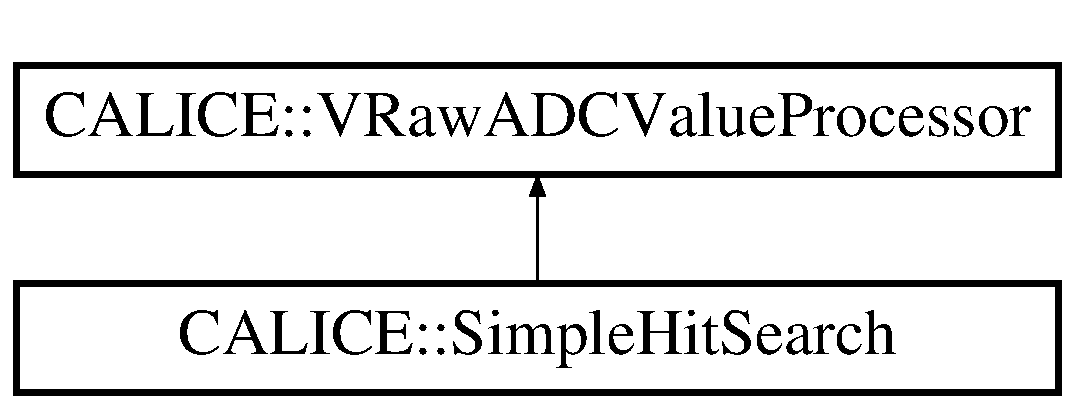
\includegraphics[height=2cm]{classCALICE_1_1SimpleHitSearch}
\end{center}
\end{figure}
\subsection*{Public Member Functions}
\begin{DoxyCompactItemize}
\item 
Processor $\ast$ {\bf newProcessor} ()\label{classCALICE_1_1SimpleHitSearch_a9c6691eab502152d7d480b9b9fdc8118}

\begin{DoxyCompactList}\small\item\em construct a new Processor (required by Marlin. \item\end{DoxyCompactList}\item 
{\bf SimpleHitSearch} ()
\begin{DoxyCompactList}\small\item\em default constructor. \item\end{DoxyCompactList}\item 
{\bf $\sim$SimpleHitSearch} ()\label{classCALICE_1_1SimpleHitSearch_a2f968c5e21b3e6dee9f2ad4d4021f840}

\begin{DoxyCompactList}\small\item\em destructor. \item\end{DoxyCompactList}\item 
void {\bf init} ()
\begin{DoxyCompactList}\small\item\em Called at the begin of the job before anything is read. \item\end{DoxyCompactList}\item 
void {\bf processRunHeader} (LCRunHeader $\ast$run)
\begin{DoxyCompactList}\small\item\em Called for every run (does nothing. \item\end{DoxyCompactList}\item 
void {\bf processEvent} (LCEvent $\ast$evtP)
\begin{DoxyCompactList}\small\item\em Calculate Pedestals and Noise and search and reconstruct calorimeter hits. \item\end{DoxyCompactList}\item 
void {\bfseries end} ()\label{classCALICE_1_1SimpleHitSearch_a80eecd952cd8813fdb95885a2066f899}

\end{DoxyCompactItemize}
\subsection*{Static Public Member Functions}
\begin{DoxyCompactItemize}
\item 
static {\bf NoiseParameterArray\_\-t} \& {\bfseries getCellParameters} ()\label{classCALICE_1_1SimpleHitSearch_afcf3db2cdd66d984735fed6dea5dccef}

\end{DoxyCompactItemize}
\subsection*{Protected Types}
\begin{DoxyCompactItemize}
\item 
enum {\bf EState} \{ \par
{\bf kStateUnknown}, 
{\bf kStateSkipEvent}, 
{\bf kStateCosmics}, 
{\bf kStateBeam}, 
\par
{\bf kStatePedestals}, 
{\bf kStateInitialPedestals}, 
{\bf kStateRefinePedestals}, 
{\bf kStateCalibration}, 
\par
{\bfseries kNStates}
 \}
\item 
typedef void(SimpleHitSearch::$\ast$ {\bfseries ProcessFunc\_\-t} )(EVENT::LCEvent $\ast$evtP)\label{classCALICE_1_1SimpleHitSearch_a45197af7f9a68676066cebde627f4cfc}

\end{DoxyCompactItemize}
\subsection*{Protected Member Functions}
\begin{DoxyCompactItemize}
\item 
void {\bf changeState} ({\bf EState} new\_\-state)\label{classCALICE_1_1SimpleHitSearch_a4446f9d98f8e27263dbc1407454e9a9a}

\begin{DoxyCompactList}\small\item\em Change the state to the one specified. \item\end{DoxyCompactList}\item 
bool {\bf stateTransition} ()
\begin{DoxyCompactList}\small\item\em Change the state. \item\end{DoxyCompactList}\item 
void {\bf callStateFunc} (LCEvent $\ast$evtP)
\begin{DoxyCompactList}\small\item\em Call the event processing functions of the current state (state function). \item\end{DoxyCompactList}\item 
void {\bf skipEvents} (LCEvent $\ast$evtP)
\begin{DoxyCompactList}\small\item\em Skip events. \item\end{DoxyCompactList}\item 
void {\bf processCosmics} (LCEvent $\ast$evtP)
\begin{DoxyCompactList}\small\item\em Process cosmics events. \item\end{DoxyCompactList}\item 
void {\bf processBeamEvents} (LCEvent $\ast$evtP)
\begin{DoxyCompactList}\small\item\em Process beam events. \item\end{DoxyCompactList}\item 
void {\bf processPedestalEvents} (LCEvent $\ast$evtP)
\begin{DoxyCompactList}\small\item\em Process pedestal events. \item\end{DoxyCompactList}\item 
void {\bf processFirstPedestalEvents} (LCEvent $\ast$evtP)
\begin{DoxyCompactList}\small\item\em Process events to get the first idea of the pedestals. \item\end{DoxyCompactList}\item 
void {\bf processPedestalEventsWithHitRejection} (LCEvent $\ast$evtP)
\begin{DoxyCompactList}\small\item\em Refine the initial guess of the pedestals. \item\end{DoxyCompactList}\item 
void {\bf skipCalibrationEvents} (LCEvent $\ast$evtP)
\begin{DoxyCompactList}\small\item\em Skip events for which the calibration chip is on. \item\end{DoxyCompactList}\item 
void {\bf fullReset} ()\label{classCALICE_1_1SimpleHitSearch_a52c65040ce64c64e5d85b1e9bb9deb58}

\begin{DoxyCompactList}\small\item\em Reset the arrays which contain the pedestals and the noise, hit counter etc. \item\end{DoxyCompactList}\item 
void {\bf resetForInitialPedestalNoiseCalculation} ()\label{classCALICE_1_1SimpleHitSearch_a5469f7b4a5daeb02dde42785a971fa27}

\begin{DoxyCompactList}\small\item\em Initialise the pedestal/noise arrays for the initial pedestal/noise estimate. \item\end{DoxyCompactList}\item 
void {\bf resetForPedestalNoiseReCalculation} ()\label{classCALICE_1_1SimpleHitSearch_a9f507aa7f979b24fcb339c20f09be0c7}

\begin{DoxyCompactList}\small\item\em Initialise the pedestal/noise arrays for the pedestal/noise estimate (An initial pedestal/noise estimate is assumed). \item\end{DoxyCompactList}\item 
void {\bfseries resetHitCounter} ()\label{classCALICE_1_1SimpleHitSearch_ac15a138546477596a59bec83320d0209}

\item 
void {\bfseries resetSaturationCounter} ()\label{classCALICE_1_1SimpleHitSearch_a88b5ade283b9c3ed356cd55800f05119}

\item 
void {\bf accumulateEventsForInitialPedestalNoiseCalculation} (LCEvent $\ast$evtP)
\begin{DoxyCompactList}\small\item\em Accumulate data to calculate pedestals and the noise. \item\end{DoxyCompactList}\item 
void {\bf accumulateEventsForPedestalNoiseCalculationWithHitRejection} (LCEvent $\ast$evtP)
\begin{DoxyCompactList}\small\item\em Accumulate data to calculate pedestals and the noise with hit rejection. \item\end{DoxyCompactList}\item 
void {\bf accumulateEventsForPedestalNoiseCalculationWithHitRejectionAndPedestalShiftDetection} (LCEvent $\ast$evtP)
\begin{DoxyCompactList}\small\item\em Accumulate data to calculate pedestals and the noise. \item\end{DoxyCompactList}\item 
void {\bf calculatePedestalNoiseAndDeclareCellsDead} ()
\begin{DoxyCompactList}\small\item\em Calculate pedestals and noise using the gathered information of the accumalted events. \item\end{DoxyCompactList}\item 
void {\bf searchHits} (LCEvent $\ast$evt)
\begin{DoxyCompactList}\small\item\em Search hits without adjusting noise and pedestals (suitable for test beam data). \item\end{DoxyCompactList}\item 
void {\bf searchHitsAndAdjustPedestalsAndNoise} (LCEvent $\ast$evtP)
\begin{DoxyCompactList}\small\item\em Search hits and adjust the pedestal and noise of cells with a signal below the cut \_\-signalCut (suitable for cosmics data). \item\end{DoxyCompactList}\item 
void {\bf buildCellParameters} ()
\begin{DoxyCompactList}\small\item\em Create and initialise the array which will contain for all cells the pedestals and the noise and further status information. \item\end{DoxyCompactList}\item 
void {\bf showNoiseStat} () const \label{classCALICE_1_1SimpleHitSearch_a244abb0f99096175c8b9264fcbee6d46}

\begin{DoxyCompactList}\small\item\em Show per layer statistics about the noise and the pedestals. \item\end{DoxyCompactList}\item 
void {\bf showCurrentNoiseStat} () const 
\begin{DoxyCompactList}\small\item\em Show per layer statistics about the noise and the pedestals (during pedestal noise accumulation). \item\end{DoxyCompactList}\item 
Float\_\-t {\bf calculatePedestalCorrection} (UInt\_\-t module\_\-i, Float\_\-t $\ast$adc\_\-values\_\-per\_\-module) const 
\begin{DoxyCompactList}\small\item\em calculculate an average pedestal correction for one module. \item\end{DoxyCompactList}\item 
{\bf vector}$<$ Float\_\-t $>$ {\bfseries calculateSignalInducedPedestalCorrection} (UInt\_\-t module\_\-i, const Float\_\-t $\ast$adc\_\-values\_\-per\_\-module) const \label{classCALICE_1_1SimpleHitSearch_a168ec110d0f6529ed97052137ea8c173}

\item 
Float\_\-t {\bfseries getCalibratedValue} (UInt\_\-t module\_\-index, UInt\_\-t cell\_\-index, Float\_\-t pedestal\_\-subtracted\_\-adc\_\-value) const \label{classCALICE_1_1SimpleHitSearch_a7c3abb75e490a3f20eb4f6b53e87d9b3}

\end{DoxyCompactItemize}
\subsection*{Protected Attributes}
\begin{DoxyCompactItemize}
\item 
ProcessFunc\_\-t {\bfseries \_\-stateFunc} [kNStates]\label{classCALICE_1_1SimpleHitSearch_a7665760485119e27ea4792fb43fff838}

\item 
ProcessFunc\_\-t {\bfseries \_\-theStateFunc}\label{classCALICE_1_1SimpleHitSearch_a395561a17ee6269f8317f072205579dc}

\item 
{\bf EState} {\bfseries \_\-isState}\label{classCALICE_1_1SimpleHitSearch_ab9f1f866bb2c2d15a887a6a2271602ea}

\end{DoxyCompactItemize}
\subsection*{Private Member Functions}
\begin{DoxyCompactItemize}
\item 
void {\bfseries moduleTypeChanged} (lcio::LCCollection $\ast$col)\label{classCALICE_1_1SimpleHitSearch_a9fd889599491aea14d850439b1c0f47a}

\item 
void {\bfseries moduleLocationChanged} (lcio::LCCollection $\ast$col)\label{classCALICE_1_1SimpleHitSearch_a7e6b8d77c3b761bfb2dd44066a5c77ba}

\item 
void {\bfseries detectorTransformationChanged} (lcio::LCCollection $\ast$col)\label{classCALICE_1_1SimpleHitSearch_a9c7c2d1e9591a2e9666f7b09debf8290}

\item 
void {\bfseries referenceTransformationChanged} (lcio::LCCollection $\ast$col)\label{classCALICE_1_1SimpleHitSearch_a9ac5d578b5d61d3bf3e6836ce81d50d8}

\end{DoxyCompactItemize}
\subsection*{Private Attributes}
\begin{DoxyCompactItemize}
\item 
bool {\bfseries \_\-pedestalNoiseIsKnown}\label{classCALICE_1_1SimpleHitSearch_a5a67c59ddfe5fecf37f6ffff62e367f3}

\item 
{\bf Calibration} $\ast$ {\bfseries \_\-calibration}\label{classCALICE_1_1SimpleHitSearch_a48ee55effb72a72a2ae2f0ba3cc98b86}

\item 
TriggerBits {\bf \_\-triggerConf}
\begin{DoxyCompactList}\small\item\em Variable which contains the current trigger configuration. \item\end{DoxyCompactList}\item 
TriggerBits {\bf \_\-lastTriggerConf}
\begin{DoxyCompactList}\small\item\em Variable which contains the trigger configuration of the previous event. \item\end{DoxyCompactList}\item 
TriggerBits {\bf \_\-triggerEvent}
\begin{DoxyCompactList}\small\item\em Variable which contains the current trigger main word. \item\end{DoxyCompactList}\item 
LCCollection $\ast$ {\bfseries \_\-cellParameterCollection}\label{classCALICE_1_1SimpleHitSearch_a21aaa5e445083d41e36c0c18330a7b1f}

\item 
std::string {\bfseries \_\-cellParameterCollectionName}\label{classCALICE_1_1SimpleHitSearch_a4f5bae03c05e7c7dca47eb296123fd6f}

\item 
{\bf CellParameterArray\_\-t} {\bfseries \_\-cellParameter}\label{classCALICE_1_1SimpleHitSearch_ae0d3dfb82159643faa7c372491846f35}

\item 
RunInformation {\bfseries \_\-runInfo}\label{classCALICE_1_1SimpleHitSearch_ada8feaedebde89fbd964230993f57856}

\item 
int {\bfseries \_\-runnum}\label{classCALICE_1_1SimpleHitSearch_a11f16d75717fd4d37b0bea1a4a5b4248}

\item 
TFile $\ast$ {\bfseries \_\-hfile}\label{classCALICE_1_1SimpleHitSearch_aa86e3dadf02048636966923b9c59de25}

\item 
TH1F $\ast$ {\bfseries p\_\-Ped} [30][9][36]\label{classCALICE_1_1SimpleHitSearch_aa093649773a7d6cae7a14f1f137f096e}

\item 
bool {\bfseries \_\-isDead} [30][9][36]\label{classCALICE_1_1SimpleHitSearch_a202bb40612bf67dd94e26403a3d98107}

\item 
IntVec {\bfseries \_\-adcRange}\label{classCALICE_1_1SimpleHitSearch_ac2d20692aaf6148938c7b5308a6b3f76}

\item 
FloatVec {\bfseries \_\-noiseRange}\label{classCALICE_1_1SimpleHitSearch_a44e34d5fe8fc48f6867ccf3e11668549}

\item 
FloatVec {\bfseries \_\-pedestalRange}\label{classCALICE_1_1SimpleHitSearch_a16637f5a59e2056537556f021fc9922b}

\item 
Float\_\-t {\bfseries \_\-pedestalChangeCut}\label{classCALICE_1_1SimpleHitSearch_a67bc48aa8bbbf0a9a22c94383338c4d9}

\item 
Float\_\-t {\bf \_\-maxPedestalChange}
\begin{DoxyCompactList}\small\item\em Maximum allowed pedestal change. \item\end{DoxyCompactList}\item 
Int\_\-t {\bfseries \_\-removeMaximumInNEvents}\label{classCALICE_1_1SimpleHitSearch_af010bd49f78718fb2ac7d53e467df172}

\item 
Float\_\-t {\bf \_\-maxHitOccupancy}
\begin{DoxyCompactList}\small\item\em Maximum number of tolerated hits. \item\end{DoxyCompactList}\item 
Int\_\-t {\bf \_\-minNEventsForPedestalNoiseUpdate}
\begin{DoxyCompactList}\small\item\em Minimum number of events to be accumulated before the pedestals and noise are calculated (parameter). \item\end{DoxyCompactList}\item 
Int\_\-t {\bf \_\-updatePedestalsEveryNEvents}
\begin{DoxyCompactList}\small\item\em Update pedestals every n events, during pedestal triggers. \item\end{DoxyCompactList}\item 
Int\_\-t {\bf \_\-weightOfOldPedestalNoise}
\begin{DoxyCompactList}\small\item\em Weight given to old pedestals and noise when using a new value to adjust the pedestals and the noise (parameter). \item\end{DoxyCompactList}\item 
Float\_\-t {\bf \_\-shiftPedestalFactor}
\begin{DoxyCompactList}\small\item\em When processing pedestal events, shift pedestals by average values measured on one module times this factor. \item\end{DoxyCompactList}\item 
Int\_\-t {\bf \_\-skipFirstNEvents}
\begin{DoxyCompactList}\small\item\em Skip the first n events (parameter). \item\end{DoxyCompactList}\item 
Int\_\-t {\bf \_\-skipNEventsAfterConfChanges}
\begin{DoxyCompactList}\small\item\em Skip n events after configuration changes (parameter). \item\end{DoxyCompactList}\item 
Int\_\-t {\bf \_\-skipNEvents}
\begin{DoxyCompactList}\small\item\em Skip the next n events (not a parameter). \item\end{DoxyCompactList}\item 
Int\_\-t {\bf \_\-skipCalibrationEventsAlways}
\begin{DoxyCompactList}\small\item\em Skip events in which the calibration chip was turned on. \item\end{DoxyCompactList}\item 
Int\_\-t {\bf \_\-skipNEventsAfterSlowConfRecords}
\begin{DoxyCompactList}\small\item\em Events skipped after slow or configuration records. \item\end{DoxyCompactList}\item 
Int\_\-t {\bf \_\-skipDirtyEventsInPedestalCalculation}
\begin{DoxyCompactList}\small\item\em Events skipped during pedestal calculation because they are considered to be dirty. \item\end{DoxyCompactList}\item 
Float\_\-t {\bfseries \_\-toleratedSaturationFraction}\label{classCALICE_1_1SimpleHitSearch_aee3c0be45f5ad8bacf4be69adc7243c9}

\item 
Float\_\-t {\bf \_\-signalThreshold}
\begin{DoxyCompactList}\small\item\em Signals above the signal threshold and . \item\end{DoxyCompactList}\item 
FloatVec {\bf \_\-noiseCutVec}
\begin{DoxyCompactList}\small\item\em above the noise cut are considered to be hits. \item\end{DoxyCompactList}\item 
Float\_\-t {\bf \_\-noiseCut}\label{classCALICE_1_1SimpleHitSearch_a43d55978859ed6e08879c8fbcec51fe4}

\begin{DoxyCompactList}\small\item\em will be set by the first element of the \_\-noiseCutVec \item\end{DoxyCompactList}\item 
Float\_\-t {\bf \_\-noiseCutForPedestalNoiseCalculation}
\begin{DoxyCompactList}\small\item\em will be set by the second element of the \_\-noiseCutVec (if available). \item\end{DoxyCompactList}\item 
int {\bf \_\-nNegativeSignalsPerModule}
\begin{DoxyCompactList}\small\item\em maximum number of negative signals per module. \item\end{DoxyCompactList}\item 
std::string {\bf \_\-hitColName}
\begin{DoxyCompactList}\small\item\em Name of the hit collection (OUTPUT). \item\end{DoxyCompactList}\item 
std::string {\bf \_\-rawhitColName}
\begin{DoxyCompactList}\small\item\em Name of the raw hit collection (optional OUTPUT). \item\end{DoxyCompactList}\item 
bool {\bf \_\-writeRawHits}
\begin{DoxyCompactList}\small\item\em Save the output collection containing RawCalorimeterHits. \item\end{DoxyCompactList}\item 
bool {\bf \_\-saveEcalNoise}
\begin{DoxyCompactList}\small\item\em Save the Noise value in the database. \item\end{DoxyCompactList}\item 
std::string {\bf \_\-dbInit}\label{classCALICE_1_1SimpleHitSearch_a171f19ba1537593d58af925d3fd37af5}

\begin{DoxyCompactList}\small\item\em DBInit string. \item\end{DoxyCompactList}\item 
std::string {\bf \_\-folderNoise}\label{classCALICE_1_1SimpleHitSearch_a2768a3edd7f2a10dd62bd27744153212}

\begin{DoxyCompactList}\small\item\em Variable containing folder name for Ecal Noise. \item\end{DoxyCompactList}\item 
std::string {\bf \_\-colNameDetectorTransformation}
\begin{DoxyCompactList}\small\item\em Name of the conditions data collection which describes the position and the rotation of the detector. \item\end{DoxyCompactList}\item 
std::string {\bf \_\-colNameReferenceTransformation}
\begin{DoxyCompactList}\small\item\em Name of the conditions data collection which describes the reference position and rotation. \item\end{DoxyCompactList}\item 
std::string {\bf \_\-calibrationObjectName}\label{classCALICE_1_1SimpleHitSearch_a0a9b79f36130b7634a968757204106c4}

\begin{DoxyCompactList}\small\item\em Name of the \doxyref{Calibration}{p.}{classCalibration} object to be used (will be created using the \doxyref{CalibrationFactory}{p.}{classCalibrationFactory}). \item\end{DoxyCompactList}\item 
std::string {\bf \_\-calibrationConstantColName}
\begin{DoxyCompactList}\small\item\em Name of the conditions data collection containing the calibration constants. \item\end{DoxyCompactList}\item 
std::string {\bf \_\-parNameTriggerConf}
\begin{DoxyCompactList}\small\item\em Name of the event parameter which contains the current trigger configuration. \item\end{DoxyCompactList}\item 
std::string {\bf \_\-parNameTriggerEvent}
\begin{DoxyCompactList}\small\item\em Name of the event parameter which contains the current trigger main word. \item\end{DoxyCompactList}\item 
std::string {\bfseries \_\-parNameTriggerPreHistory}\label{classCALICE_1_1SimpleHitSearch_aa830de5cd9ecf215fd4c8f7dabb89905}

\item 
std::string {\bfseries \_\-parNameTriggerPostHistory}\label{classCALICE_1_1SimpleHitSearch_a101a94c7e3cebda25d572372a299242a}

\item 
std::string {\bf \_\-parNameRecoState}
\begin{DoxyCompactList}\small\item\em Name of the event parameter which will be filled with the current state of the reconstruction. \item\end{DoxyCompactList}\item 
std::string {\bf \_\-parNameEventEnergy}
\begin{DoxyCompactList}\small\item\em Parameter name of the event energy. \item\end{DoxyCompactList}\item 
std::string {\bf \_\-parNamePedestalCorrection}
\begin{DoxyCompactList}\small\item\em Parameter name of the event energy. \item\end{DoxyCompactList}\item 
ConditionsChangeDelegator$<$ {\bf SimpleHitSearch} $>$ {\bf \_\-detectorTransformationChange}
\begin{DoxyCompactList}\small\item\em helper class to listen for changes of the detector position or rotation. \item\end{DoxyCompactList}\item 
ConditionsChangeDelegator$<$ {\bf SimpleHitSearch} $>$ {\bf \_\-referenceTransformationChange}
\begin{DoxyCompactList}\small\item\em helper class to listen for changes of the reference position or rotation. \item\end{DoxyCompactList}\item 
UInt\_\-t {\bfseries \_\-nPedestalEvents}\label{classCALICE_1_1SimpleHitSearch_a52fab5d22925a91d926f48cc9738c91a}

\item 
UInt\_\-t {\bfseries \_\-nPedestalEventsTotal}\label{classCALICE_1_1SimpleHitSearch_a028bae6980be7a807f1653c62ca6cea9}

\item 
UInt\_\-t {\bfseries \_\-nPedestalEventSets}\label{classCALICE_1_1SimpleHitSearch_ab1d4f9b957aba4b42682785f29203570}

\item 
UInt\_\-t {\bfseries \_\-nEvents}\label{classCALICE_1_1SimpleHitSearch_a8380b2ba839ba192f158f0b2dd5b2595}

\item 
UInt\_\-t {\bfseries \_\-nEventsTotal}\label{classCALICE_1_1SimpleHitSearch_aa1a9621e79f38d26546a4484741aa2e9}

\item 
UInt\_\-t {\bfseries \_\-nEventsWithHits}\label{classCALICE_1_1SimpleHitSearch_a037a41dd3ccbde0ba5c4f7c5b192efde}

\item 
UInt\_\-t {\bfseries \_\-nEventsWithHitsTotal}\label{classCALICE_1_1SimpleHitSearch_a96c924a9b98d261504b89f741cb733a6}

\item 
UInt\_\-t {\bfseries \_\-nEventsSkipped}\label{classCALICE_1_1SimpleHitSearch_ac807f9dd96f4fcac703b4c9c0ba4ed4f}

\item 
UInt\_\-t {\bfseries \_\-eventCounterForMaximumRejection}\label{classCALICE_1_1SimpleHitSearch_a37ec85fa6893b07d56dc9781151a344c}

\item 
UInt\_\-t {\bfseries \_\-uncoveredTriggerCounter}\label{classCALICE_1_1SimpleHitSearch_ad2548d5d0c666f6cf4ba7314e93e825a}

\item 
UInt\_\-t {\bfseries \_\-nEventsWithoutADC}\label{classCALICE_1_1SimpleHitSearch_a4d545f53fc92d3fa9b9d79aaf6ae654a}

\item 
UInt\_\-t {\bfseries \_\-rejectedEvents}\label{classCALICE_1_1SimpleHitSearch_acc168ae78c41be89f0ec797fbcd5a9e7}

\item 
UInt\_\-t {\bfseries \_\-rejectBecauseOfError}\label{classCALICE_1_1SimpleHitSearch_aeed4d4e7089c0be06e943d7fe016a93e}

\item 
UInt\_\-t {\bfseries \_\-rejectBecauseTooManyHits}\label{classCALICE_1_1SimpleHitSearch_a57e713ebf5c905d6ed3ee081ac7c878a}

\item 
UInt\_\-t {\bfseries \_\-rejectBecauseOfMissingADCBlocks}\label{classCALICE_1_1SimpleHitSearch_a3544a9c8fa07c39cce41fc061152a32f}

\item 
UInt\_\-t {\bfseries \_\-nEventsWithMissingAdcBlocks}\label{classCALICE_1_1SimpleHitSearch_ac3691afbd7bb89347d19ce73df8cae9a}

\item 
Int\_\-t {\bfseries \_\-viewConnectionTree}\label{classCALICE_1_1SimpleHitSearch_a892f40de556066455a63575f0c0247d6}

\item 
{\bf vector}$<$ Float\_\-t $>$ {\bfseries \_\-moduleBuffer}\label{classCALICE_1_1SimpleHitSearch_ab854d696c8a7ddf18cd18eab248900ef}

\item 
{\bf vector}$<$ Float\_\-t $>$ {\bfseries \_\-avNoisePerModule}\label{classCALICE_1_1SimpleHitSearch_a621e4afdc02db8d42adf197986f889d0}

\item 
lcio::StringVec {\bf \_\-maskedErrorNames}
\begin{DoxyCompactList}\small\item\em Names of alle masked errors (proc. \item\end{DoxyCompactList}\item 
unsigned int {\bf \_\-errorMask}
\begin{DoxyCompactList}\small\item\em bit mask of all errors to be ignored. \item\end{DoxyCompactList}\item 
Bool\_\-t {\bfseries \_\-calibrationOn}\label{classCALICE_1_1SimpleHitSearch_a24d9bfec50160d0071bce65b0dbd0d7d}

\item 
UInt\_\-t {\bfseries \_\-lastEvent}\label{classCALICE_1_1SimpleHitSearch_a1cb4d8110b9d02187b62dcb0737092b3}

\end{DoxyCompactItemize}


\subsection{Detailed Description}
Marlin Processor to search and reconstruct colorimeter hits. The hits are selected using a signal-\/over-\/noise threshold or a signal threshold (can be chosen at compile time by defining the environment variable (FIXED\_\-THRESHOLD -\/$>$ signal threshold). The class takes care of the pedestal and noise calculation. The hit position is calculated using information stored in a LCCD conditions database. Moreover, the signal is calibrated if a proper calibration object exists. Currently, there is only the \doxyref{NoOpCalibration}{p.}{classNoOpCalibration} which does nothing. 

Definition at line 46 of file SimpleHitSearch.hh.

\subsection{Member Enumeration Documentation}
\index{CALICE::SimpleHitSearch@{CALICE::SimpleHitSearch}!EState@{EState}}
\index{EState@{EState}!CALICE::SimpleHitSearch@{CALICE::SimpleHitSearch}}
\subsubsection[{EState}]{\setlength{\rightskip}{0pt plus 5cm}enum {\bf CALICE::SimpleHitSearch::EState}\hspace{0.3cm}{\ttfamily  [protected]}}\label{classCALICE_1_1SimpleHitSearch_a26a3d0d7abf5b4511990ed16d1964ad1}
\begin{Desc}
\item[Enumerator: ]\par
\begin{description}
\index{kStateUnknown@{kStateUnknown}!CALICE::SimpleHitSearch@{CALICE::SimpleHitSearch}}\index{CALICE::SimpleHitSearch@{CALICE::SimpleHitSearch}!kStateUnknown@{kStateUnknown}}\item[{\em 
kStateUnknown\label{classCALICE_1_1SimpleHitSearch_a26a3d0d7abf5b4511990ed16d1964ad1a747f2b548416998e817796f90575aba7}
}]0: unknown state. \index{kStateSkipEvent@{kStateSkipEvent}!CALICE::SimpleHitSearch@{CALICE::SimpleHitSearch}}\index{CALICE::SimpleHitSearch@{CALICE::SimpleHitSearch}!kStateSkipEvent@{kStateSkipEvent}}\item[{\em 
kStateSkipEvent\label{classCALICE_1_1SimpleHitSearch_a26a3d0d7abf5b4511990ed16d1964ad1a325fe5f2f04499d334162bfcce8512d7}
}]1: events are skipped unprocessed. \index{kStateCosmics@{kStateCosmics}!CALICE::SimpleHitSearch@{CALICE::SimpleHitSearch}}\index{CALICE::SimpleHitSearch@{CALICE::SimpleHitSearch}!kStateCosmics@{kStateCosmics}}\item[{\em 
kStateCosmics\label{classCALICE_1_1SimpleHitSearch_a26a3d0d7abf5b4511990ed16d1964ad1a31a96472fae4e02ab6dab5a2ef100b29}
}]2: events are treated as cosmics (low, signals at random locations). \index{kStateBeam@{kStateBeam}!CALICE::SimpleHitSearch@{CALICE::SimpleHitSearch}}\index{CALICE::SimpleHitSearch@{CALICE::SimpleHitSearch}!kStateBeam@{kStateBeam}}\item[{\em 
kStateBeam\label{classCALICE_1_1SimpleHitSearch_a26a3d0d7abf5b4511990ed16d1964ad1aa623a732bc5ea94b5bb300aaf755684b}
}]3: events are treated as beam events (high, localised signals). \index{kStatePedestals@{kStatePedestals}!CALICE::SimpleHitSearch@{CALICE::SimpleHitSearch}}\index{CALICE::SimpleHitSearch@{CALICE::SimpleHitSearch}!kStatePedestals@{kStatePedestals}}\item[{\em 
kStatePedestals\label{classCALICE_1_1SimpleHitSearch_a26a3d0d7abf5b4511990ed16d1964ad1aff7721d469bfee8d8b991f577b805b95}
}]4: events are treated as pedestal/noise events (no signals). \index{kStateInitialPedestals@{kStateInitialPedestals}!CALICE::SimpleHitSearch@{CALICE::SimpleHitSearch}}\index{CALICE::SimpleHitSearch@{CALICE::SimpleHitSearch}!kStateInitialPedestals@{kStateInitialPedestals}}\item[{\em 
kStateInitialPedestals\label{classCALICE_1_1SimpleHitSearch_a26a3d0d7abf5b4511990ed16d1964ad1a04fe816441d604e962f0e3dbd254b701}
}]5: pedestals and noise are estimated assuming little signal at random locations. \index{kStateRefinePedestals@{kStateRefinePedestals}!CALICE::SimpleHitSearch@{CALICE::SimpleHitSearch}}\index{CALICE::SimpleHitSearch@{CALICE::SimpleHitSearch}!kStateRefinePedestals@{kStateRefinePedestals}}\item[{\em 
kStateRefinePedestals\label{classCALICE_1_1SimpleHitSearch_a26a3d0d7abf5b4511990ed16d1964ad1a937edad6225a7500e00a9c65e62baaee}
}]6: pedestal and noise estimates are improved assuming little signal at random locations. \index{kStateCalibration@{kStateCalibration}!CALICE::SimpleHitSearch@{CALICE::SimpleHitSearch}}\index{CALICE::SimpleHitSearch@{CALICE::SimpleHitSearch}!kStateCalibration@{kStateCalibration}}\item[{\em 
kStateCalibration\label{classCALICE_1_1SimpleHitSearch_a26a3d0d7abf5b4511990ed16d1964ad1aae90af32fec9607b3807b2959d7f0002}
}]7: There are permanent (calibration) signals at specific locations . \end{description}
\end{Desc}



Definition at line 97 of file SimpleHitSearch.hh.

\subsection{Constructor \& Destructor Documentation}
\index{CALICE::SimpleHitSearch@{CALICE::SimpleHitSearch}!SimpleHitSearch@{SimpleHitSearch}}
\index{SimpleHitSearch@{SimpleHitSearch}!CALICE::SimpleHitSearch@{CALICE::SimpleHitSearch}}
\subsubsection[{SimpleHitSearch}]{\setlength{\rightskip}{0pt plus 5cm}CALICE::SimpleHitSearch::SimpleHitSearch ()}\label{classCALICE_1_1SimpleHitSearch_a878f8268e15a16efa94ebbfc79e74250}


default constructor. defines and registers its parameters. 

Definition at line 67 of file SimpleHitSearch.cc.

References \_\-calibrationConstantColName, \_\-calibrationObjectName, \_\-colNameDetectorTransformation, \_\-colNameReferenceTransformation, \_\-dbInit, \_\-folderNoise, \_\-hitColName, \_\-maskedErrorNames, \_\-maxHitOccupancy, \_\-maxPedestalChange, \_\-minNEventsForPedestalNoiseUpdate, \_\-noiseCutVec, \_\-parNameEventEnergy, \_\-parNamePedestalCorrection, \_\-parNameRecoState, \_\-parNameTriggerConf, \_\-parNameTriggerEvent, \_\-rawhitColName, \_\-saveEcalNoise, \_\-shiftPedestalFactor, \_\-signalThreshold, \_\-skipCalibrationEventsAlways, \_\-skipFirstNEvents, \_\-skipNEventsAfterConfChanges, \_\-skipNEventsAfterSlowConfRecords, \_\-updatePedestalsEveryNEvents, \_\-weightOfOldPedestalNoise, \_\-writeRawHits, changeState(), kStateBeam, kStateCalibration, kStateCosmics, kStateInitialPedestals, kStatePedestals, kStateRefinePedestals, kStateSkipEvent, kStateUnknown, processBeamEvents(), processCosmics(), processFirstPedestalEvents(), processPedestalEvents(), processPedestalEventsWithHitRejection(), and skipEvents().

\subsection{Member Function Documentation}
\index{CALICE::SimpleHitSearch@{CALICE::SimpleHitSearch}!accumulateEventsForInitialPedestalNoiseCalculation@{accumulateEventsForInitialPedestalNoiseCalculation}}
\index{accumulateEventsForInitialPedestalNoiseCalculation@{accumulateEventsForInitialPedestalNoiseCalculation}!CALICE::SimpleHitSearch@{CALICE::SimpleHitSearch}}
\subsubsection[{accumulateEventsForInitialPedestalNoiseCalculation}]{\setlength{\rightskip}{0pt plus 5cm}void CALICE::SimpleHitSearch::accumulateEventsForInitialPedestalNoiseCalculation (LCEvent $\ast$ {\em evtP})\hspace{0.3cm}{\ttfamily  [protected]}}\label{classCALICE_1_1SimpleHitSearch_adce6351652d1d9fe70198c3da5c7e3b9}


Accumulate data to calculate pedestals and the noise. It is assumed that the event sample does not contain any hits. Otherwise The noise and the pedestals will be biased to larger values. 

Definition at line 1326 of file SimpleHitSearch.cc.

References CALICE::VRawADCValueProcessor::\_\-adcColName, CALICE::CellParameter::add(), buildCellParameters(), CALICE::CellParameter::getMaxValue(), CALICE::CellParameter::incrementSaturationCounter(), CALICE::CellParameter::isDead(), CALICE::CellParameter::setMaxValue(), and CALICE::CellParameter::sub().

Referenced by processFirstPedestalEvents().\index{CALICE::SimpleHitSearch@{CALICE::SimpleHitSearch}!accumulateEventsForPedestalNoiseCalculationWithHitRejection@{accumulateEventsForPedestalNoiseCalculationWithHitRejection}}
\index{accumulateEventsForPedestalNoiseCalculationWithHitRejection@{accumulateEventsForPedestalNoiseCalculationWithHitRejection}!CALICE::SimpleHitSearch@{CALICE::SimpleHitSearch}}
\subsubsection[{accumulateEventsForPedestalNoiseCalculationWithHitRejection}]{\setlength{\rightskip}{0pt plus 5cm}void CALICE::SimpleHitSearch::accumulateEventsForPedestalNoiseCalculationWithHitRejection (LCEvent $\ast$ {\em evtP})\hspace{0.3cm}{\ttfamily  [protected]}}\label{classCALICE_1_1SimpleHitSearch_a066ec6c399d4e557457da357acdfb7db}


Accumulate data to calculate pedestals and the noise with hit rejection. Values which are above the threshold \_\-signalCutForPedestalNoiseCalculation are not considered in the pedestal and noise calculation. If the threshold is too low the pedestals and the noise will be biased to lower values. If the threshold is too high and there are many hits the pedestals and the noise will be biased to higher values. This method is suitable for events with little amount of hits which are clearly separated from the pedestals. 

Definition at line 1394 of file SimpleHitSearch.cc.

References CALICE::VRawADCValueProcessor::\_\-adcColName, \_\-noiseCutForPedestalNoiseCalculation, \_\-shiftPedestalFactor, CALICE::CellParameter::add(), buildCellParameters(), CALICE::CellParameter::getNoise(), CALICE::CellParameter::getPedestal(), CALICE::CellParameter::incrementSaturationCounter(), and CALICE::CellParameter::isDead().

Referenced by processBeamEvents(), processPedestalEvents(), and processPedestalEventsWithHitRejection().\index{CALICE::SimpleHitSearch@{CALICE::SimpleHitSearch}!accumulateEventsForPedestalNoiseCalculationWithHitRejectionAndPedestalShiftDetection@{accumulateEventsForPedestalNoiseCalculationWithHitRejectionAndPedestalShiftDetection}}
\index{accumulateEventsForPedestalNoiseCalculationWithHitRejectionAndPedestalShiftDetection@{accumulateEventsForPedestalNoiseCalculationWithHitRejectionAndPedestalShiftDetection}!CALICE::SimpleHitSearch@{CALICE::SimpleHitSearch}}
\subsubsection[{accumulateEventsForPedestalNoiseCalculationWithHitRejectionAndPedestalShiftDetection}]{\setlength{\rightskip}{0pt plus 5cm}void CALICE::SimpleHitSearch::accumulateEventsForPedestalNoiseCalculationWithHitRejectionAndPedestalShiftDetection (LCEvent $\ast$ {\em evtP})\hspace{0.3cm}{\ttfamily  [protected]}}\label{classCALICE_1_1SimpleHitSearch_a8f264ece7366955c1d742954a28a4d0d}


Accumulate data to calculate pedestals and the noise. If the pedestal shifts by more than the threshold \_\-pedestalChangeCut than the old pedestal is shifted. As a consequence the precision on the pedestal is lousy, the noise may be biased to lower values. This method is suitable for noise events which were taken over a long periode which suffers large and discrete shifts of the pedestals. \begin{Desc}
\item[{\bf Todo}]useful? \end{Desc}
\begin{DoxySeeAlso}{See also}
\doxyref{calculatePedestalNoiseAndDeclareCellsDead}{p.}{classCALICE_1_1SimpleHitSearch_a9b72dcaf97a6ec7cb0bb7904df96e0ac} 
\end{DoxySeeAlso}


Definition at line 1474 of file SimpleHitSearch.cc.

References CALICE::VRawADCValueProcessor::\_\-adcColName, \_\-noiseCutForPedestalNoiseCalculation, CALICE::CellParameter::add(), buildCellParameters(), CALICE::CellParameter::getMeanADCValue(), CALICE::CellParameter::getNoise(), CALICE::CellParameter::getPedestal(), CALICE::CellParameter::incrementSaturationCounter(), CALICE::CellParameter::isDead(), and CALICE::CellParameter::shiftPedestal().\index{CALICE::SimpleHitSearch@{CALICE::SimpleHitSearch}!buildCellParameters@{buildCellParameters}}
\index{buildCellParameters@{buildCellParameters}!CALICE::SimpleHitSearch@{CALICE::SimpleHitSearch}}
\subsubsection[{buildCellParameters}]{\setlength{\rightskip}{0pt plus 5cm}void CALICE::SimpleHitSearch::buildCellParameters ()\hspace{0.3cm}{\ttfamily  [protected]}}\label{classCALICE_1_1SimpleHitSearch_a6d16f225e1eb6f4b913200f56e9dfc57}


Create and initialise the array which will contain for all cells the pedestals and the noise and further status information. \begin{DoxySeeAlso}{See also}
\doxyref{CellParameter}{p.}{classCALICE_1_1CellParameter} 
\end{DoxySeeAlso}


Definition at line 2519 of file SimpleHitSearch.cc.

References Calibration::checkForCalibrationConstantsOfModule(), and Calibration::isValid().

Referenced by accumulateEventsForInitialPedestalNoiseCalculation(), accumulateEventsForPedestalNoiseCalculationWithHitRejection(), accumulateEventsForPedestalNoiseCalculationWithHitRejectionAndPedestalShiftDetection(), searchHits(), and searchHitsAndAdjustPedestalsAndNoise().\index{CALICE::SimpleHitSearch@{CALICE::SimpleHitSearch}!calculatePedestalCorrection@{calculatePedestalCorrection}}
\index{calculatePedestalCorrection@{calculatePedestalCorrection}!CALICE::SimpleHitSearch@{CALICE::SimpleHitSearch}}
\subsubsection[{calculatePedestalCorrection}]{\setlength{\rightskip}{0pt plus 5cm}Float\_\-t CALICE::SimpleHitSearch::calculatePedestalCorrection (UInt\_\-t {\em module\_\-i}, \/  Float\_\-t $\ast$ {\em adc\_\-values\_\-per\_\-module}) const\hspace{0.3cm}{\ttfamily  [protected]}}\label{classCALICE_1_1SimpleHitSearch_a5b4e48cd1fbaa73067f273222cbc7e2b}


calculculate an average pedestal correction for one module. 
\begin{DoxyParams}{Parameters}
\item[{\em module\_\-i}]the module index \item[{\em adc\_\-values\_\-per\_\-module}]an array which has for each cell of the module one adc value or -\/FLT\_\-MAX for dead cells. \end{DoxyParams}
\begin{DoxyReturn}{Returns}
an additive correction which should be applied to all pedestals of the module. 
\end{DoxyReturn}


Definition at line 2828 of file SimpleHitSearch.cc.

Referenced by searchHits().\index{CALICE::SimpleHitSearch@{CALICE::SimpleHitSearch}!calculatePedestalNoiseAndDeclareCellsDead@{calculatePedestalNoiseAndDeclareCellsDead}}
\index{calculatePedestalNoiseAndDeclareCellsDead@{calculatePedestalNoiseAndDeclareCellsDead}!CALICE::SimpleHitSearch@{CALICE::SimpleHitSearch}}
\subsubsection[{calculatePedestalNoiseAndDeclareCellsDead}]{\setlength{\rightskip}{0pt plus 5cm}void CALICE::SimpleHitSearch::calculatePedestalNoiseAndDeclareCellsDead ()\hspace{0.3cm}{\ttfamily  [protected]}}\label{classCALICE_1_1SimpleHitSearch_a9b72dcaf97a6ec7cb0bb7904df96e0ac}


Calculate pedestals and noise using the gathered information of the accumalted events. \begin{DoxySeeAlso}{See also}
\doxyref{accumulateEventsForInitialPedestalNoiseCalculation}{p.}{classCALICE_1_1SimpleHitSearch_adce6351652d1d9fe70198c3da5c7e3b9}, \doxyref{accumulateEventsForPedestalNoiseCalculationWithHitRejection}{p.}{classCALICE_1_1SimpleHitSearch_a066ec6c399d4e557457da357acdfb7db}, \doxyref{accumulateEventsForPedestalNoiseCalculationWithHitRejectionAndPedestalShiftDetection}{p.}{classCALICE_1_1SimpleHitSearch_a8f264ece7366955c1d742954a28a4d0d} 
\end{DoxySeeAlso}


Definition at line 1540 of file SimpleHitSearch.cc.

References \_\-maxPedestalChange, CALICE::CellParameter::calculate(), histmgr::HistMgr::getHistogramCollection(), CALICE::CellParameter::getNoise(), CALICE::CellParameter::getPedestal(), CALICE::CellParameter::getSaturationCounter(), histmgr::HistogramCollection\_\-t::histogram(), CALICE::CellParameter::isDead(), and CALICE::CellParameter::setDead().

Referenced by processPedestalEvents(), and stateTransition().\index{CALICE::SimpleHitSearch@{CALICE::SimpleHitSearch}!callStateFunc@{callStateFunc}}
\index{callStateFunc@{callStateFunc}!CALICE::SimpleHitSearch@{CALICE::SimpleHitSearch}}
\subsubsection[{callStateFunc}]{\setlength{\rightskip}{0pt plus 5cm}void CALICE::SimpleHitSearch::callStateFunc (LCEvent $\ast$ {\em evtP})\hspace{0.3cm}{\ttfamily  [inline, protected]}}\label{classCALICE_1_1SimpleHitSearch_a5872fdf70fc02008f755641dece7b3a9}


Call the event processing functions of the current state (state function). \begin{DoxySeeAlso}{See also}
\doxyref{skipEvents}{p.}{classCALICE_1_1SimpleHitSearch_a2e726ffcd5de61d365e75ddd4049bb44}, \doxyref{processCosmics}{p.}{classCALICE_1_1SimpleHitSearch_a9b4fd80a9bfc4fe67cc5b724764dfd16}, \doxyref{processBeamEvents}{p.}{classCALICE_1_1SimpleHitSearch_a5bf0ed4df472053477e6333726d25c14}, \doxyref{processPedestalEvents}{p.}{classCALICE_1_1SimpleHitSearch_a0cc31eedb3dca01bf3e232f0ae4a38cb}, \doxyref{processFirstPedestalEvents}{p.}{classCALICE_1_1SimpleHitSearch_a20cca077ae4ef0fac2eeb2cddb05cd1e} 

\doxyref{processPedestalEventsWithHitRejection}{p.}{classCALICE_1_1SimpleHitSearch_aaea180512610968f84a512c81d3198ea}, \doxyref{skipCalibrationEvents}{p.}{classCALICE_1_1SimpleHitSearch_a0172933d2cbc9807fa5ddcef99b63a41}, 
\end{DoxySeeAlso}


Definition at line 130 of file SimpleHitSearch.hh.

Referenced by processBeamEvents(), processCosmics(), processEvent(), processFirstPedestalEvents(), processPedestalEventsWithHitRejection(), skipCalibrationEvents(), and skipEvents().\index{CALICE::SimpleHitSearch@{CALICE::SimpleHitSearch}!init@{init}}
\index{init@{init}!CALICE::SimpleHitSearch@{CALICE::SimpleHitSearch}}
\subsubsection[{init}]{\setlength{\rightskip}{0pt plus 5cm}void CALICE::SimpleHitSearch::init ()}\label{classCALICE_1_1SimpleHitSearch_ad0e512445dcbad98d4fd8129ccf9236e}


Called at the begin of the job before anything is read. Use to initialize the processor, e.g. book histograms. 

Reimplemented from {\bf CALICE::VRawADCValueProcessor} \doxyref{}{p.}{classCALICE_1_1VRawADCValueProcessor}.

Definition at line 484 of file SimpleHitSearch.cc.

References \_\-calibrationConstantColName, \_\-calibrationObjectName, \_\-colNameDetectorTransformation, CALICE::VRawADCValueProcessor::\_\-colNameModuleDescription, \_\-colNameReferenceTransformation, \_\-detectorTransformationChange, \_\-errorMask, \_\-maskedErrorNames, \_\-minNEventsForPedestalNoiseUpdate, \_\-noiseCut, \_\-noiseCutForPedestalNoiseCalculation, \_\-noiseCutVec, \_\-parNameEventEnergy, \_\-referenceTransformationChange, \_\-skipCalibrationEventsAlways, \_\-skipDirtyEventsInPedestalCalculation, \_\-skipFirstNEvents, \_\-skipNEvents, \_\-updatePedestalsEveryNEvents, changeState(), CalibrationFactory::createCalibrationObject(), histmgr::HistMgr::createHistogramGroup(), fullReset(), CalibrationFactory::getInstance(), kStateCalibration, kStateSkipEvent, CalibrationFactory::listKits(), histmgr::HistMgr::lockGroup(), and skipCalibrationEvents().\index{CALICE::SimpleHitSearch@{CALICE::SimpleHitSearch}!processBeamEvents@{processBeamEvents}}
\index{processBeamEvents@{processBeamEvents}!CALICE::SimpleHitSearch@{CALICE::SimpleHitSearch}}
\subsubsection[{processBeamEvents}]{\setlength{\rightskip}{0pt plus 5cm}void CALICE::SimpleHitSearch::processBeamEvents (LCEvent $\ast$ {\em evtP})\hspace{0.3cm}{\ttfamily  [protected]}}\label{classCALICE_1_1SimpleHitSearch_a5bf0ed4df472053477e6333726d25c14}


Process beam events. State function called if \_\-isState = kStateBeam or if kStateCalibration (configurable). 

Definition at line 961 of file SimpleHitSearch.cc.

References \_\-triggerConf, \_\-triggerEvent, accumulateEventsForPedestalNoiseCalculationWithHitRejection(), callStateFunc(), searchHits(), and stateTransition().

Referenced by SimpleHitSearch().\index{CALICE::SimpleHitSearch@{CALICE::SimpleHitSearch}!processCosmics@{processCosmics}}
\index{processCosmics@{processCosmics}!CALICE::SimpleHitSearch@{CALICE::SimpleHitSearch}}
\subsubsection[{processCosmics}]{\setlength{\rightskip}{0pt plus 5cm}void CALICE::SimpleHitSearch::processCosmics (LCEvent $\ast$ {\em evtP})\hspace{0.3cm}{\ttfamily  [protected]}}\label{classCALICE_1_1SimpleHitSearch_a9b4fd80a9bfc4fe67cc5b724764dfd16}


Process cosmics events. State function called if \_\-isState = kStateCosmics. 

Definition at line 948 of file SimpleHitSearch.cc.

References \_\-triggerConf, callStateFunc(), searchHitsAndAdjustPedestalsAndNoise(), and stateTransition().

Referenced by SimpleHitSearch().\index{CALICE::SimpleHitSearch@{CALICE::SimpleHitSearch}!processEvent@{processEvent}}
\index{processEvent@{processEvent}!CALICE::SimpleHitSearch@{CALICE::SimpleHitSearch}}
\subsubsection[{processEvent}]{\setlength{\rightskip}{0pt plus 5cm}void CALICE::SimpleHitSearch::processEvent (LCEvent $\ast$ {\em evtP})}\label{classCALICE_1_1SimpleHitSearch_a2b66e493c061a1977fb6e1bb1da6bbb0}


Calculate Pedestals and Noise and search and reconstruct calorimeter hits. The class needs as input the ADC value collection and produces a CalorimeterHit collection. 

Depending on the trigger configuration, the pedestal and noise are either calculated from random triggers (test beam data) or it is assumed that the hit distribution is sparse and randomly distributed over the detector (cosmics data). In the latter case the pedestals and noise are calculated initially from the first events assuming the events do not contain any hits. Then, the initial guess is slowly adjusted. Otherwise the pedestals and the noise are calculted from pedestal events.

The event processing method depends on the state (\doxyref{EState}{p.}{classCALICE_1_1SimpleHitSearch_a26a3d0d7abf5b4511990ed16d1964ad1}) of the analysis. The state transition is trigger by trigger configuration changes, changes of the calibration chip configuration, knowledge about the pedestals and noise. \begin{DoxySeeAlso}{See also}
searchHit 

ssearchHitsAndAdjustPedestalsAndNoise, \doxyref{stateTransition}{p.}{classCALICE_1_1SimpleHitSearch_a360d0e7f063d7a2706edc2a59113caa9} 
\end{DoxySeeAlso}


Definition at line 1186 of file SimpleHitSearch.cc.

References \_\-parNameRecoState, \_\-parNameTriggerConf, \_\-parNameTriggerEvent, \_\-skipNEvents, \_\-skipNEventsAfterConfChanges, \_\-skipNEventsAfterSlowConfRecords, \_\-triggerConf, \_\-triggerEvent, callStateFunc(), changeState(), histmgr::HistMgr::getHistogramCollection(), histmgr::HistogramCollection\_\-t::histogram(), kStateSkipEvent, and stateTransition().\index{CALICE::SimpleHitSearch@{CALICE::SimpleHitSearch}!processFirstPedestalEvents@{processFirstPedestalEvents}}
\index{processFirstPedestalEvents@{processFirstPedestalEvents}!CALICE::SimpleHitSearch@{CALICE::SimpleHitSearch}}
\subsubsection[{processFirstPedestalEvents}]{\setlength{\rightskip}{0pt plus 5cm}void CALICE::SimpleHitSearch::processFirstPedestalEvents (LCEvent $\ast$ {\em evtP})\hspace{0.3cm}{\ttfamily  [protected]}}\label{classCALICE_1_1SimpleHitSearch_a20cca077ae4ef0fac2eeb2cddb05cd1e}


Process events to get the first idea of the pedestals. State function called if the pedestal and noise is not yet known and if the events are either pedestal or cosmics events. 

Definition at line 1002 of file SimpleHitSearch.cc.

References \_\-minNEventsForPedestalNoiseUpdate, \_\-skipDirtyEventsInPedestalCalculation, \_\-triggerEvent, accumulateEventsForInitialPedestalNoiseCalculation(), callStateFunc(), and stateTransition().

Referenced by SimpleHitSearch().\index{CALICE::SimpleHitSearch@{CALICE::SimpleHitSearch}!processPedestalEvents@{processPedestalEvents}}
\index{processPedestalEvents@{processPedestalEvents}!CALICE::SimpleHitSearch@{CALICE::SimpleHitSearch}}
\subsubsection[{processPedestalEvents}]{\setlength{\rightskip}{0pt plus 5cm}void CALICE::SimpleHitSearch::processPedestalEvents (LCEvent $\ast$ {\em evtP})\hspace{0.3cm}{\ttfamily  [protected]}}\label{classCALICE_1_1SimpleHitSearch_a0cc31eedb3dca01bf3e232f0ae4a38cb}


Process pedestal events. State function called if \_\-isState = kStatePedestals 

Definition at line 979 of file SimpleHitSearch.cc.

References \_\-skipDirtyEventsInPedestalCalculation, \_\-triggerEvent, \_\-updatePedestalsEveryNEvents, accumulateEventsForPedestalNoiseCalculationWithHitRejection(), calculatePedestalNoiseAndDeclareCellsDead(), and resetForPedestalNoiseReCalculation().

Referenced by SimpleHitSearch().\index{CALICE::SimpleHitSearch@{CALICE::SimpleHitSearch}!processPedestalEventsWithHitRejection@{processPedestalEventsWithHitRejection}}
\index{processPedestalEventsWithHitRejection@{processPedestalEventsWithHitRejection}!CALICE::SimpleHitSearch@{CALICE::SimpleHitSearch}}
\subsubsection[{processPedestalEventsWithHitRejection}]{\setlength{\rightskip}{0pt plus 5cm}void CALICE::SimpleHitSearch::processPedestalEventsWithHitRejection (LCEvent $\ast$ {\em evtP})\hspace{0.3cm}{\ttfamily  [protected]}}\label{classCALICE_1_1SimpleHitSearch_aaea180512610968f84a512c81d3198ea}


Refine the initial guess of the pedestals. State function called subsequent to \doxyref{processFirstPedestalEvents}{p.}{classCALICE_1_1SimpleHitSearch_a20cca077ae4ef0fac2eeb2cddb05cd1e} and if the events are either pedestal or cosmics events. 

Definition at line 1027 of file SimpleHitSearch.cc.

References \_\-minNEventsForPedestalNoiseUpdate, \_\-skipDirtyEventsInPedestalCalculation, \_\-triggerEvent, accumulateEventsForPedestalNoiseCalculationWithHitRejection(), callStateFunc(), and stateTransition().

Referenced by SimpleHitSearch().\index{CALICE::SimpleHitSearch@{CALICE::SimpleHitSearch}!processRunHeader@{processRunHeader}}
\index{processRunHeader@{processRunHeader}!CALICE::SimpleHitSearch@{CALICE::SimpleHitSearch}}
\subsubsection[{processRunHeader}]{\setlength{\rightskip}{0pt plus 5cm}void CALICE::SimpleHitSearch::processRunHeader (LCRunHeader $\ast$ {\em run})}\label{classCALICE_1_1SimpleHitSearch_a67696ee27a7da8b2e3df2ece1024bd36}


Called for every run (does nothing. ) 

Definition at line 621 of file SimpleHitSearch.cc.\index{CALICE::SimpleHitSearch@{CALICE::SimpleHitSearch}!searchHits@{searchHits}}
\index{searchHits@{searchHits}!CALICE::SimpleHitSearch@{CALICE::SimpleHitSearch}}
\subsubsection[{searchHits}]{\setlength{\rightskip}{0pt plus 5cm}void CALICE::SimpleHitSearch::searchHits (LCEvent $\ast$ {\em evt})\hspace{0.3cm}{\ttfamily  [protected]}}\label{classCALICE_1_1SimpleHitSearch_ad905e8e0f57ae2263f5d733e0f5d8081}


Search hits without adjusting noise and pedestals (suitable for test beam data). This method is only useful in cases in which cells rarely contain hits (like cosmics data). Test beam data usually has hits always at the same place. 
\begin{DoxyParams}{Parameters}
\item[{\em evt}]pointer to a event which contains the ADC value collection. \end{DoxyParams}


Definition at line 1676 of file SimpleHitSearch.cc.

References CALICE::VRawADCValueProcessor::\_\-adcColName, \_\-errorMask, \_\-maxHitOccupancy, \_\-maxPedestalChange, \_\-noiseCut, \_\-parNameEventEnergy, \_\-parNamePedestalCorrection, \_\-rawhitColName, \_\-signalThreshold, \_\-writeRawHits, buildCellParameters(), calculatePedestalCorrection(), histmgr::HistMgr::getHistogram2DCollection(), histmgr::HistMgr::getHistogramCollection(), Calibration::getMiniumADCForMipThreshold(), CALICE::CellParameter::getNoise(), CALICE::CellParameter::getPedestal(), histmgr::Histogram2DCollection\_\-t::histogram(), histmgr::HistogramCollection\_\-t::histogram(), CALICE::CellParameter::incrementNHits(), CALICE::CellParameter::incrementSaturationCounter(), CALICE::CellParameter::isDead(), histmgr::Histogram2DCollection\_\-t::n(), CALICE::NoiseParameter::setDead(), CALICE::NoiseParameter::setGeomCellIndex(), CALICE::NoiseParameter::setNoise(), CALICE::CellParameter::setOldPedestal(), CALICE::NoiseParameter::setPedestal(), CALICE::CellParameter::setPedestal(), CALICE::NoiseParameter::setPedestalBeforeGC(), and CALICE::NoiseParameter::setPedestalBeforeSIC().

Referenced by processBeamEvents().\index{CALICE::SimpleHitSearch@{CALICE::SimpleHitSearch}!searchHitsAndAdjustPedestalsAndNoise@{searchHitsAndAdjustPedestalsAndNoise}}
\index{searchHitsAndAdjustPedestalsAndNoise@{searchHitsAndAdjustPedestalsAndNoise}!CALICE::SimpleHitSearch@{CALICE::SimpleHitSearch}}
\subsubsection[{searchHitsAndAdjustPedestalsAndNoise}]{\setlength{\rightskip}{0pt plus 5cm}void CALICE::SimpleHitSearch::searchHitsAndAdjustPedestalsAndNoise (LCEvent $\ast$ {\em evtP})\hspace{0.3cm}{\ttfamily  [protected]}}\label{classCALICE_1_1SimpleHitSearch_abfaa7aa6a94bcca3541094148f9623a6}


Search hits and adjust the pedestal and noise of cells with a signal below the cut \_\-signalCut (suitable for cosmics data). This method is only useful in cases in which cells rarely contain hits (like cosmics data). Test beam data usually has hits always at the same place. 
\begin{DoxyParams}{Parameters}
\item[{\em evtP}]pointer to a event which contains the ADC value collection. \end{DoxyParams}


Definition at line 2278 of file SimpleHitSearch.cc.

References CALICE::VRawADCValueProcessor::\_\-adcColName, \_\-errorMask, \_\-hitColName, \_\-maxHitOccupancy, \_\-noiseCut, \_\-signalThreshold, \_\-weightOfOldPedestalNoise, CALICE::CellParameter::adjustPedestalNoise(), buildCellParameters(), CALICE::NVector\_\-t$<$ T, dimension $>$::data(), histmgr::HistMgr::getHistogramCollection(), Calibration::getMiniumADCForMipThreshold(), CALICE::CellParameter::getNoise(), CALICE::CellParameter::getOldNoise(), CALICE::CellParameter::getOldPedestal(), CALICE::CellParameter::getPedestal(), histmgr::HistogramCollection\_\-t::histogram(), CALICE::CellParameter::incrementNHits(), CALICE::CellParameter::incrementSaturationCounter(), and CALICE::CellParameter::isDead().

Referenced by processCosmics().\index{CALICE::SimpleHitSearch@{CALICE::SimpleHitSearch}!showCurrentNoiseStat@{showCurrentNoiseStat}}
\index{showCurrentNoiseStat@{showCurrentNoiseStat}!CALICE::SimpleHitSearch@{CALICE::SimpleHitSearch}}
\subsubsection[{showCurrentNoiseStat}]{\setlength{\rightskip}{0pt plus 5cm}void CALICE::SimpleHitSearch::showCurrentNoiseStat () const\hspace{0.3cm}{\ttfamily  [protected]}}\label{classCALICE_1_1SimpleHitSearch_ad59226d349f2168a7eec3e9ff04a8f10}


Show per layer statistics about the noise and the pedestals (during pedestal noise accumulation). This method calculates the pedestals and the noise itself from the accumulated sums. Will show incorrect results after the pedestals and the noise have been calculated. 

Definition at line 1651 of file SimpleHitSearch.cc.

References CALICE::CellParameter::getNValues(), CALICE::CellParameter::getOldNoise(), CALICE::CellParameter::getOldPedestal(), and CALICE::CellParameter::isDead().\index{CALICE::SimpleHitSearch@{CALICE::SimpleHitSearch}!skipCalibrationEvents@{skipCalibrationEvents}}
\index{skipCalibrationEvents@{skipCalibrationEvents}!CALICE::SimpleHitSearch@{CALICE::SimpleHitSearch}}
\subsubsection[{skipCalibrationEvents}]{\setlength{\rightskip}{0pt plus 5cm}void CALICE::SimpleHitSearch::skipCalibrationEvents (LCEvent $\ast$ {\em evtP})\hspace{0.3cm}{\ttfamily  [protected]}}\label{classCALICE_1_1SimpleHitSearch_a0172933d2cbc9807fa5ddcef99b63a41}


Skip events for which the calibration chip is on. State function which skip events until the calibration chip is switched off (configurable). 

Definition at line 937 of file SimpleHitSearch.cc.

References \_\-triggerConf, callStateFunc(), and stateTransition().

Referenced by init().\index{CALICE::SimpleHitSearch@{CALICE::SimpleHitSearch}!skipEvents@{skipEvents}}
\index{skipEvents@{skipEvents}!CALICE::SimpleHitSearch@{CALICE::SimpleHitSearch}}
\subsubsection[{skipEvents}]{\setlength{\rightskip}{0pt plus 5cm}void CALICE::SimpleHitSearch::skipEvents (LCEvent $\ast$ {\em evtP})\hspace{0.3cm}{\ttfamily  [protected]}}\label{classCALICE_1_1SimpleHitSearch_a2e726ffcd5de61d365e75ddd4049bb44}


Skip events. State function called for the first n events (configurable) and for n events after configuration changes. 

Definition at line 923 of file SimpleHitSearch.cc.

References \_\-skipNEvents, \_\-triggerConf, callStateFunc(), and stateTransition().

Referenced by SimpleHitSearch().\index{CALICE::SimpleHitSearch@{CALICE::SimpleHitSearch}!stateTransition@{stateTransition}}
\index{stateTransition@{stateTransition}!CALICE::SimpleHitSearch@{CALICE::SimpleHitSearch}}
\subsubsection[{stateTransition}]{\setlength{\rightskip}{0pt plus 5cm}bool CALICE::SimpleHitSearch::stateTransition ()\hspace{0.3cm}{\ttfamily  [protected]}}\label{classCALICE_1_1SimpleHitSearch_a360d0e7f063d7a2706edc2a59113caa9}


Change the state. return true if the state changed. 

Definition at line 1052 of file SimpleHitSearch.cc.

References \_\-minNEventsForPedestalNoiseUpdate, \_\-skipNEvents, \_\-triggerConf, calculatePedestalNoiseAndDeclareCellsDead(), changeState(), histmgr::HistMgr::getHistogramCollection(), histmgr::HistogramCollection\_\-t::histogram(), kStateBeam, kStateCalibration, kStateCosmics, kStateInitialPedestals, kStatePedestals, kStateRefinePedestals, kStateSkipEvent, resetForInitialPedestalNoiseCalculation(), resetForPedestalNoiseReCalculation(), and showNoiseStat().

Referenced by processBeamEvents(), processCosmics(), processEvent(), processFirstPedestalEvents(), processPedestalEventsWithHitRejection(), skipCalibrationEvents(), and skipEvents().

\subsection{Field Documentation}
\index{CALICE::SimpleHitSearch@{CALICE::SimpleHitSearch}!\_\-calibrationConstantColName@{\_\-calibrationConstantColName}}
\index{\_\-calibrationConstantColName@{\_\-calibrationConstantColName}!CALICE::SimpleHitSearch@{CALICE::SimpleHitSearch}}
\subsubsection[{\_\-calibrationConstantColName}]{\setlength{\rightskip}{0pt plus 5cm}std::string {\bf CALICE::SimpleHitSearch::\_\-calibrationConstantColName}\hspace{0.3cm}{\ttfamily  [private]}}\label{classCALICE_1_1SimpleHitSearch_aef43b966b83d8ec305748ddabf257bc9}


Name of the conditions data collection containing the calibration constants. 

Definition at line 357 of file SimpleHitSearch.hh.

Referenced by init(), and SimpleHitSearch().\index{CALICE::SimpleHitSearch@{CALICE::SimpleHitSearch}!\_\-colNameDetectorTransformation@{\_\-colNameDetectorTransformation}}
\index{\_\-colNameDetectorTransformation@{\_\-colNameDetectorTransformation}!CALICE::SimpleHitSearch@{CALICE::SimpleHitSearch}}
\subsubsection[{\_\-colNameDetectorTransformation}]{\setlength{\rightskip}{0pt plus 5cm}std::string {\bf CALICE::SimpleHitSearch::\_\-colNameDetectorTransformation}\hspace{0.3cm}{\ttfamily  [private]}}\label{classCALICE_1_1SimpleHitSearch_aea8b3f66ad9dc9343e260eea7eb47076}


Name of the conditions data collection which describes the position and the rotation of the detector. 

Definition at line 351 of file SimpleHitSearch.hh.

Referenced by init(), and SimpleHitSearch().\index{CALICE::SimpleHitSearch@{CALICE::SimpleHitSearch}!\_\-colNameReferenceTransformation@{\_\-colNameReferenceTransformation}}
\index{\_\-colNameReferenceTransformation@{\_\-colNameReferenceTransformation}!CALICE::SimpleHitSearch@{CALICE::SimpleHitSearch}}
\subsubsection[{\_\-colNameReferenceTransformation}]{\setlength{\rightskip}{0pt plus 5cm}std::string {\bf CALICE::SimpleHitSearch::\_\-colNameReferenceTransformation}\hspace{0.3cm}{\ttfamily  [private]}}\label{classCALICE_1_1SimpleHitSearch_a8896eddafd13fd917f87f3d6aabe25e9}


Name of the conditions data collection which describes the reference position and rotation. 

Definition at line 353 of file SimpleHitSearch.hh.

Referenced by init(), and SimpleHitSearch().\index{CALICE::SimpleHitSearch@{CALICE::SimpleHitSearch}!\_\-detectorTransformationChange@{\_\-detectorTransformationChange}}
\index{\_\-detectorTransformationChange@{\_\-detectorTransformationChange}!CALICE::SimpleHitSearch@{CALICE::SimpleHitSearch}}
\subsubsection[{\_\-detectorTransformationChange}]{\setlength{\rightskip}{0pt plus 5cm}ConditionsChangeDelegator$<${\bf SimpleHitSearch}$>$ {\bf CALICE::SimpleHitSearch::\_\-detectorTransformationChange}\hspace{0.3cm}{\ttfamily  [private]}}\label{classCALICE_1_1SimpleHitSearch_aa4299d9a2ade3995ff2bab83b8649f3e}


helper class to listen for changes of the detector position or rotation. 

Definition at line 373 of file SimpleHitSearch.hh.

Referenced by init().\index{CALICE::SimpleHitSearch@{CALICE::SimpleHitSearch}!\_\-errorMask@{\_\-errorMask}}
\index{\_\-errorMask@{\_\-errorMask}!CALICE::SimpleHitSearch@{CALICE::SimpleHitSearch}}
\subsubsection[{\_\-errorMask}]{\setlength{\rightskip}{0pt plus 5cm}unsigned int {\bf CALICE::SimpleHitSearch::\_\-errorMask}\hspace{0.3cm}{\ttfamily  [private]}}\label{classCALICE_1_1SimpleHitSearch_a87087b542fdabc0b4243ec4fe4b81202}


bit mask of all errors to be ignored. 

Definition at line 458 of file SimpleHitSearch.hh.

Referenced by init(), searchHits(), and searchHitsAndAdjustPedestalsAndNoise().\index{CALICE::SimpleHitSearch@{CALICE::SimpleHitSearch}!\_\-hitColName@{\_\-hitColName}}
\index{\_\-hitColName@{\_\-hitColName}!CALICE::SimpleHitSearch@{CALICE::SimpleHitSearch}}
\subsubsection[{\_\-hitColName}]{\setlength{\rightskip}{0pt plus 5cm}std::string {\bf CALICE::SimpleHitSearch::\_\-hitColName}\hspace{0.3cm}{\ttfamily  [private]}}\label{classCALICE_1_1SimpleHitSearch_a69bf745ec5aed1df895972b78aa7e15e}


Name of the hit collection (OUTPUT). 

Definition at line 342 of file SimpleHitSearch.hh.

Referenced by searchHitsAndAdjustPedestalsAndNoise(), and SimpleHitSearch().\index{CALICE::SimpleHitSearch@{CALICE::SimpleHitSearch}!\_\-lastTriggerConf@{\_\-lastTriggerConf}}
\index{\_\-lastTriggerConf@{\_\-lastTriggerConf}!CALICE::SimpleHitSearch@{CALICE::SimpleHitSearch}}
\subsubsection[{\_\-lastTriggerConf}]{\setlength{\rightskip}{0pt plus 5cm}TriggerBits {\bf CALICE::SimpleHitSearch::\_\-lastTriggerConf}\hspace{0.3cm}{\ttfamily  [private]}}\label{classCALICE_1_1SimpleHitSearch_ae834049eda6ad568ea644ec3b0283783}


Variable which contains the trigger configuration of the previous event. 

Definition at line 282 of file SimpleHitSearch.hh.\index{CALICE::SimpleHitSearch@{CALICE::SimpleHitSearch}!\_\-maskedErrorNames@{\_\-maskedErrorNames}}
\index{\_\-maskedErrorNames@{\_\-maskedErrorNames}!CALICE::SimpleHitSearch@{CALICE::SimpleHitSearch}}
\subsubsection[{\_\-maskedErrorNames}]{\setlength{\rightskip}{0pt plus 5cm}lcio::StringVec {\bf CALICE::SimpleHitSearch::\_\-maskedErrorNames}\hspace{0.3cm}{\ttfamily  [private]}}\label{classCALICE_1_1SimpleHitSearch_a81e19a0434630e7f88e447b459fc6759}


Names of alle masked errors (proc. parameter) 

Definition at line 457 of file SimpleHitSearch.hh.

Referenced by init(), and SimpleHitSearch().\index{CALICE::SimpleHitSearch@{CALICE::SimpleHitSearch}!\_\-maxHitOccupancy@{\_\-maxHitOccupancy}}
\index{\_\-maxHitOccupancy@{\_\-maxHitOccupancy}!CALICE::SimpleHitSearch@{CALICE::SimpleHitSearch}}
\subsubsection[{\_\-maxHitOccupancy}]{\setlength{\rightskip}{0pt plus 5cm}Float\_\-t {\bf CALICE::SimpleHitSearch::\_\-maxHitOccupancy}\hspace{0.3cm}{\ttfamily  [private]}}\label{classCALICE_1_1SimpleHitSearch_acd7bf1c8fd19a5dc8ee5de76862fcab3}


Maximum number of tolerated hits. Events with more hits are rejected (parameter). 

Definition at line 309 of file SimpleHitSearch.hh.

Referenced by searchHits(), searchHitsAndAdjustPedestalsAndNoise(), and SimpleHitSearch().\index{CALICE::SimpleHitSearch@{CALICE::SimpleHitSearch}!\_\-maxPedestalChange@{\_\-maxPedestalChange}}
\index{\_\-maxPedestalChange@{\_\-maxPedestalChange}!CALICE::SimpleHitSearch@{CALICE::SimpleHitSearch}}
\subsubsection[{\_\-maxPedestalChange}]{\setlength{\rightskip}{0pt plus 5cm}Float\_\-t {\bf CALICE::SimpleHitSearch::\_\-maxPedestalChange}\hspace{0.3cm}{\ttfamily  [private]}}\label{classCALICE_1_1SimpleHitSearch_a7560d7eda24ea39936723d858f54cdad}


Maximum allowed pedestal change. 

Definition at line 305 of file SimpleHitSearch.hh.

Referenced by calculatePedestalNoiseAndDeclareCellsDead(), searchHits(), and SimpleHitSearch().\index{CALICE::SimpleHitSearch@{CALICE::SimpleHitSearch}!\_\-minNEventsForPedestalNoiseUpdate@{\_\-minNEventsForPedestalNoiseUpdate}}
\index{\_\-minNEventsForPedestalNoiseUpdate@{\_\-minNEventsForPedestalNoiseUpdate}!CALICE::SimpleHitSearch@{CALICE::SimpleHitSearch}}
\subsubsection[{\_\-minNEventsForPedestalNoiseUpdate}]{\setlength{\rightskip}{0pt plus 5cm}Int\_\-t {\bf CALICE::SimpleHitSearch::\_\-minNEventsForPedestalNoiseUpdate}\hspace{0.3cm}{\ttfamily  [private]}}\label{classCALICE_1_1SimpleHitSearch_a6b7f69836f9b26f0fa09819d2614d6a0}


Minimum number of events to be accumulated before the pedestals and noise are calculated (parameter). 

Definition at line 312 of file SimpleHitSearch.hh.

Referenced by init(), processFirstPedestalEvents(), processPedestalEventsWithHitRejection(), SimpleHitSearch(), and stateTransition().\index{CALICE::SimpleHitSearch@{CALICE::SimpleHitSearch}!\_\-nNegativeSignalsPerModule@{\_\-nNegativeSignalsPerModule}}
\index{\_\-nNegativeSignalsPerModule@{\_\-nNegativeSignalsPerModule}!CALICE::SimpleHitSearch@{CALICE::SimpleHitSearch}}
\subsubsection[{\_\-nNegativeSignalsPerModule}]{\setlength{\rightskip}{0pt plus 5cm}int {\bf CALICE::SimpleHitSearch::\_\-nNegativeSignalsPerModule}\hspace{0.3cm}{\ttfamily  [private]}}\label{classCALICE_1_1SimpleHitSearch_a62ced507029d3bef99d20e1c73444b8d}


maximum number of negative signals per module. 

Definition at line 340 of file SimpleHitSearch.hh.\index{CALICE::SimpleHitSearch@{CALICE::SimpleHitSearch}!\_\-noiseCutForPedestalNoiseCalculation@{\_\-noiseCutForPedestalNoiseCalculation}}
\index{\_\-noiseCutForPedestalNoiseCalculation@{\_\-noiseCutForPedestalNoiseCalculation}!CALICE::SimpleHitSearch@{CALICE::SimpleHitSearch}}
\subsubsection[{\_\-noiseCutForPedestalNoiseCalculation}]{\setlength{\rightskip}{0pt plus 5cm}Float\_\-t {\bf CALICE::SimpleHitSearch::\_\-noiseCutForPedestalNoiseCalculation}\hspace{0.3cm}{\ttfamily  [private]}}\label{classCALICE_1_1SimpleHitSearch_a1804b8d1678d5df652be9ef5f9e82141}


will be set by the second element of the \_\-noiseCutVec (if available). 

Definition at line 338 of file SimpleHitSearch.hh.

Referenced by accumulateEventsForPedestalNoiseCalculationWithHitRejection(), accumulateEventsForPedestalNoiseCalculationWithHitRejectionAndPedestalShiftDetection(), and init().\index{CALICE::SimpleHitSearch@{CALICE::SimpleHitSearch}!\_\-noiseCutVec@{\_\-noiseCutVec}}
\index{\_\-noiseCutVec@{\_\-noiseCutVec}!CALICE::SimpleHitSearch@{CALICE::SimpleHitSearch}}
\subsubsection[{\_\-noiseCutVec}]{\setlength{\rightskip}{0pt plus 5cm}FloatVec {\bf CALICE::SimpleHitSearch::\_\-noiseCutVec}\hspace{0.3cm}{\ttfamily  [private]}}\label{classCALICE_1_1SimpleHitSearch_a8247d67205fcdaf07592675b06809c81}


above the noise cut are considered to be hits. This vector contains a cut for the hit search and for the hit rejection during noise calculation 

Definition at line 334 of file SimpleHitSearch.hh.

Referenced by init(), and SimpleHitSearch().\index{CALICE::SimpleHitSearch@{CALICE::SimpleHitSearch}!\_\-parNameEventEnergy@{\_\-parNameEventEnergy}}
\index{\_\-parNameEventEnergy@{\_\-parNameEventEnergy}!CALICE::SimpleHitSearch@{CALICE::SimpleHitSearch}}
\subsubsection[{\_\-parNameEventEnergy}]{\setlength{\rightskip}{0pt plus 5cm}std::string {\bf CALICE::SimpleHitSearch::\_\-parNameEventEnergy}\hspace{0.3cm}{\ttfamily  [private]}}\label{classCALICE_1_1SimpleHitSearch_aa33b8c1df2b057a8b0f33ccc94a90fbc}


Parameter name of the event energy. If left blank nothing will be added. 

Definition at line 367 of file SimpleHitSearch.hh.

Referenced by init(), searchHits(), and SimpleHitSearch().\index{CALICE::SimpleHitSearch@{CALICE::SimpleHitSearch}!\_\-parNamePedestalCorrection@{\_\-parNamePedestalCorrection}}
\index{\_\-parNamePedestalCorrection@{\_\-parNamePedestalCorrection}!CALICE::SimpleHitSearch@{CALICE::SimpleHitSearch}}
\subsubsection[{\_\-parNamePedestalCorrection}]{\setlength{\rightskip}{0pt plus 5cm}std::string {\bf CALICE::SimpleHitSearch::\_\-parNamePedestalCorrection}\hspace{0.3cm}{\ttfamily  [private]}}\label{classCALICE_1_1SimpleHitSearch_aa3ca30379d46a55ac6c16a42e86abf93}


Parameter name of the event energy. If left blank nothing will be added. 

Definition at line 369 of file SimpleHitSearch.hh.

Referenced by searchHits(), and SimpleHitSearch().\index{CALICE::SimpleHitSearch@{CALICE::SimpleHitSearch}!\_\-parNameRecoState@{\_\-parNameRecoState}}
\index{\_\-parNameRecoState@{\_\-parNameRecoState}!CALICE::SimpleHitSearch@{CALICE::SimpleHitSearch}}
\subsubsection[{\_\-parNameRecoState}]{\setlength{\rightskip}{0pt plus 5cm}std::string {\bf CALICE::SimpleHitSearch::\_\-parNameRecoState}\hspace{0.3cm}{\ttfamily  [private]}}\label{classCALICE_1_1SimpleHitSearch_a5a8c2b03b3c58df9d1ad29bc33c351a7}


Name of the event parameter which will be filled with the current state of the reconstruction. 

Definition at line 365 of file SimpleHitSearch.hh.

Referenced by processEvent(), and SimpleHitSearch().\index{CALICE::SimpleHitSearch@{CALICE::SimpleHitSearch}!\_\-parNameTriggerConf@{\_\-parNameTriggerConf}}
\index{\_\-parNameTriggerConf@{\_\-parNameTriggerConf}!CALICE::SimpleHitSearch@{CALICE::SimpleHitSearch}}
\subsubsection[{\_\-parNameTriggerConf}]{\setlength{\rightskip}{0pt plus 5cm}std::string {\bf CALICE::SimpleHitSearch::\_\-parNameTriggerConf}\hspace{0.3cm}{\ttfamily  [private]}}\label{classCALICE_1_1SimpleHitSearch_ab232718833907bde19216de26bf1052d}


Name of the event parameter which contains the current trigger configuration. 

Definition at line 359 of file SimpleHitSearch.hh.

Referenced by processEvent(), and SimpleHitSearch().\index{CALICE::SimpleHitSearch@{CALICE::SimpleHitSearch}!\_\-parNameTriggerEvent@{\_\-parNameTriggerEvent}}
\index{\_\-parNameTriggerEvent@{\_\-parNameTriggerEvent}!CALICE::SimpleHitSearch@{CALICE::SimpleHitSearch}}
\subsubsection[{\_\-parNameTriggerEvent}]{\setlength{\rightskip}{0pt plus 5cm}std::string {\bf CALICE::SimpleHitSearch::\_\-parNameTriggerEvent}\hspace{0.3cm}{\ttfamily  [private]}}\label{classCALICE_1_1SimpleHitSearch_a3b05e6eec6a1a3e6f418456b11e222e0}


Name of the event parameter which contains the current trigger main word. 

Definition at line 360 of file SimpleHitSearch.hh.

Referenced by processEvent(), and SimpleHitSearch().\index{CALICE::SimpleHitSearch@{CALICE::SimpleHitSearch}!\_\-rawhitColName@{\_\-rawhitColName}}
\index{\_\-rawhitColName@{\_\-rawhitColName}!CALICE::SimpleHitSearch@{CALICE::SimpleHitSearch}}
\subsubsection[{\_\-rawhitColName}]{\setlength{\rightskip}{0pt plus 5cm}std::string {\bf CALICE::SimpleHitSearch::\_\-rawhitColName}\hspace{0.3cm}{\ttfamily  [private]}}\label{classCALICE_1_1SimpleHitSearch_afd9d15bc86011f12589ec6c8fd3bb3cc}


Name of the raw hit collection (optional OUTPUT). 

Definition at line 343 of file SimpleHitSearch.hh.

Referenced by searchHits(), and SimpleHitSearch().\index{CALICE::SimpleHitSearch@{CALICE::SimpleHitSearch}!\_\-referenceTransformationChange@{\_\-referenceTransformationChange}}
\index{\_\-referenceTransformationChange@{\_\-referenceTransformationChange}!CALICE::SimpleHitSearch@{CALICE::SimpleHitSearch}}
\subsubsection[{\_\-referenceTransformationChange}]{\setlength{\rightskip}{0pt plus 5cm}ConditionsChangeDelegator$<${\bf SimpleHitSearch}$>$ {\bf CALICE::SimpleHitSearch::\_\-referenceTransformationChange}\hspace{0.3cm}{\ttfamily  [private]}}\label{classCALICE_1_1SimpleHitSearch_a0db1b64c6e4c37cedd597d58adcf68ee}


helper class to listen for changes of the reference position or rotation. 

Definition at line 376 of file SimpleHitSearch.hh.

Referenced by init().\index{CALICE::SimpleHitSearch@{CALICE::SimpleHitSearch}!\_\-saveEcalNoise@{\_\-saveEcalNoise}}
\index{\_\-saveEcalNoise@{\_\-saveEcalNoise}!CALICE::SimpleHitSearch@{CALICE::SimpleHitSearch}}
\subsubsection[{\_\-saveEcalNoise}]{\setlength{\rightskip}{0pt plus 5cm}bool {\bf CALICE::SimpleHitSearch::\_\-saveEcalNoise}\hspace{0.3cm}{\ttfamily  [private]}}\label{classCALICE_1_1SimpleHitSearch_a9cef0868b0a1dc39b9db447df1c48a43}


Save the Noise value in the database. 

Definition at line 345 of file SimpleHitSearch.hh.

Referenced by SimpleHitSearch().\index{CALICE::SimpleHitSearch@{CALICE::SimpleHitSearch}!\_\-shiftPedestalFactor@{\_\-shiftPedestalFactor}}
\index{\_\-shiftPedestalFactor@{\_\-shiftPedestalFactor}!CALICE::SimpleHitSearch@{CALICE::SimpleHitSearch}}
\subsubsection[{\_\-shiftPedestalFactor}]{\setlength{\rightskip}{0pt plus 5cm}Float\_\-t {\bf CALICE::SimpleHitSearch::\_\-shiftPedestalFactor}\hspace{0.3cm}{\ttfamily  [private]}}\label{classCALICE_1_1SimpleHitSearch_ad5d3b9737fa5387ff8f5823a5444e052}


When processing pedestal events, shift pedestals by average values measured on one module times this factor. 

Definition at line 320 of file SimpleHitSearch.hh.

Referenced by accumulateEventsForPedestalNoiseCalculationWithHitRejection(), and SimpleHitSearch().\index{CALICE::SimpleHitSearch@{CALICE::SimpleHitSearch}!\_\-signalThreshold@{\_\-signalThreshold}}
\index{\_\-signalThreshold@{\_\-signalThreshold}!CALICE::SimpleHitSearch@{CALICE::SimpleHitSearch}}
\subsubsection[{\_\-signalThreshold}]{\setlength{\rightskip}{0pt plus 5cm}Float\_\-t {\bf CALICE::SimpleHitSearch::\_\-signalThreshold}\hspace{0.3cm}{\ttfamily  [private]}}\label{classCALICE_1_1SimpleHitSearch_a8160575528f509e54557da5e879eb6b0}


Signals above the signal threshold and . .. 

Definition at line 333 of file SimpleHitSearch.hh.

Referenced by searchHits(), searchHitsAndAdjustPedestalsAndNoise(), and SimpleHitSearch().\index{CALICE::SimpleHitSearch@{CALICE::SimpleHitSearch}!\_\-skipCalibrationEventsAlways@{\_\-skipCalibrationEventsAlways}}
\index{\_\-skipCalibrationEventsAlways@{\_\-skipCalibrationEventsAlways}!CALICE::SimpleHitSearch@{CALICE::SimpleHitSearch}}
\subsubsection[{\_\-skipCalibrationEventsAlways}]{\setlength{\rightskip}{0pt plus 5cm}Int\_\-t {\bf CALICE::SimpleHitSearch::\_\-skipCalibrationEventsAlways}\hspace{0.3cm}{\ttfamily  [private]}}\label{classCALICE_1_1SimpleHitSearch_a39ace2d2c6881e772135a918cb66c52e}


Skip events in which the calibration chip was turned on. 

Definition at line 327 of file SimpleHitSearch.hh.

Referenced by init(), and SimpleHitSearch().\index{CALICE::SimpleHitSearch@{CALICE::SimpleHitSearch}!\_\-skipDirtyEventsInPedestalCalculation@{\_\-skipDirtyEventsInPedestalCalculation}}
\index{\_\-skipDirtyEventsInPedestalCalculation@{\_\-skipDirtyEventsInPedestalCalculation}!CALICE::SimpleHitSearch@{CALICE::SimpleHitSearch}}
\subsubsection[{\_\-skipDirtyEventsInPedestalCalculation}]{\setlength{\rightskip}{0pt plus 5cm}Int\_\-t {\bf CALICE::SimpleHitSearch::\_\-skipDirtyEventsInPedestalCalculation}\hspace{0.3cm}{\ttfamily  [private]}}\label{classCALICE_1_1SimpleHitSearch_a11af8832dfb1e1176d3f982b99bf6979}


Events skipped during pedestal calculation because they are considered to be dirty. 

Definition at line 329 of file SimpleHitSearch.hh.

Referenced by init(), processFirstPedestalEvents(), processPedestalEvents(), and processPedestalEventsWithHitRejection().\index{CALICE::SimpleHitSearch@{CALICE::SimpleHitSearch}!\_\-skipFirstNEvents@{\_\-skipFirstNEvents}}
\index{\_\-skipFirstNEvents@{\_\-skipFirstNEvents}!CALICE::SimpleHitSearch@{CALICE::SimpleHitSearch}}
\subsubsection[{\_\-skipFirstNEvents}]{\setlength{\rightskip}{0pt plus 5cm}Int\_\-t {\bf CALICE::SimpleHitSearch::\_\-skipFirstNEvents}\hspace{0.3cm}{\ttfamily  [private]}}\label{classCALICE_1_1SimpleHitSearch_a2cc82196549136288114446e0507befa}


Skip the first n events (parameter). 

Definition at line 323 of file SimpleHitSearch.hh.

Referenced by init(), and SimpleHitSearch().\index{CALICE::SimpleHitSearch@{CALICE::SimpleHitSearch}!\_\-skipNEvents@{\_\-skipNEvents}}
\index{\_\-skipNEvents@{\_\-skipNEvents}!CALICE::SimpleHitSearch@{CALICE::SimpleHitSearch}}
\subsubsection[{\_\-skipNEvents}]{\setlength{\rightskip}{0pt plus 5cm}Int\_\-t {\bf CALICE::SimpleHitSearch::\_\-skipNEvents}\hspace{0.3cm}{\ttfamily  [private]}}\label{classCALICE_1_1SimpleHitSearch_ac6ccac82a60d14fb965460e822b39ab7}


Skip the next n events (not a parameter). 

Definition at line 325 of file SimpleHitSearch.hh.

Referenced by init(), processEvent(), skipEvents(), and stateTransition().\index{CALICE::SimpleHitSearch@{CALICE::SimpleHitSearch}!\_\-skipNEventsAfterConfChanges@{\_\-skipNEventsAfterConfChanges}}
\index{\_\-skipNEventsAfterConfChanges@{\_\-skipNEventsAfterConfChanges}!CALICE::SimpleHitSearch@{CALICE::SimpleHitSearch}}
\subsubsection[{\_\-skipNEventsAfterConfChanges}]{\setlength{\rightskip}{0pt plus 5cm}Int\_\-t {\bf CALICE::SimpleHitSearch::\_\-skipNEventsAfterConfChanges}\hspace{0.3cm}{\ttfamily  [private]}}\label{classCALICE_1_1SimpleHitSearch_ab8015ae646172b5c8f64becae7ff7866}


Skip n events after configuration changes (parameter). 

Definition at line 324 of file SimpleHitSearch.hh.

Referenced by processEvent(), and SimpleHitSearch().\index{CALICE::SimpleHitSearch@{CALICE::SimpleHitSearch}!\_\-skipNEventsAfterSlowConfRecords@{\_\-skipNEventsAfterSlowConfRecords}}
\index{\_\-skipNEventsAfterSlowConfRecords@{\_\-skipNEventsAfterSlowConfRecords}!CALICE::SimpleHitSearch@{CALICE::SimpleHitSearch}}
\subsubsection[{\_\-skipNEventsAfterSlowConfRecords}]{\setlength{\rightskip}{0pt plus 5cm}Int\_\-t {\bf CALICE::SimpleHitSearch::\_\-skipNEventsAfterSlowConfRecords}\hspace{0.3cm}{\ttfamily  [private]}}\label{classCALICE_1_1SimpleHitSearch_a241fbd3f423ed55a9c9678ac2004a125}


Events skipped after slow or configuration records. 

Definition at line 328 of file SimpleHitSearch.hh.

Referenced by processEvent(), and SimpleHitSearch().\index{CALICE::SimpleHitSearch@{CALICE::SimpleHitSearch}!\_\-triggerConf@{\_\-triggerConf}}
\index{\_\-triggerConf@{\_\-triggerConf}!CALICE::SimpleHitSearch@{CALICE::SimpleHitSearch}}
\subsubsection[{\_\-triggerConf}]{\setlength{\rightskip}{0pt plus 5cm}TriggerBits {\bf CALICE::SimpleHitSearch::\_\-triggerConf}\hspace{0.3cm}{\ttfamily  [private]}}\label{classCALICE_1_1SimpleHitSearch_ab4c5763d6e12c0e156f1c5dc31095acd}


Variable which contains the current trigger configuration. 

Definition at line 281 of file SimpleHitSearch.hh.

Referenced by processBeamEvents(), processCosmics(), processEvent(), skipCalibrationEvents(), skipEvents(), and stateTransition().\index{CALICE::SimpleHitSearch@{CALICE::SimpleHitSearch}!\_\-triggerEvent@{\_\-triggerEvent}}
\index{\_\-triggerEvent@{\_\-triggerEvent}!CALICE::SimpleHitSearch@{CALICE::SimpleHitSearch}}
\subsubsection[{\_\-triggerEvent}]{\setlength{\rightskip}{0pt plus 5cm}TriggerBits {\bf CALICE::SimpleHitSearch::\_\-triggerEvent}\hspace{0.3cm}{\ttfamily  [private]}}\label{classCALICE_1_1SimpleHitSearch_a2164e1d7a58f5b839c5bfe800ecab9e0}


Variable which contains the current trigger main word. 

Definition at line 284 of file SimpleHitSearch.hh.

Referenced by processBeamEvents(), processEvent(), processFirstPedestalEvents(), processPedestalEvents(), and processPedestalEventsWithHitRejection().\index{CALICE::SimpleHitSearch@{CALICE::SimpleHitSearch}!\_\-updatePedestalsEveryNEvents@{\_\-updatePedestalsEveryNEvents}}
\index{\_\-updatePedestalsEveryNEvents@{\_\-updatePedestalsEveryNEvents}!CALICE::SimpleHitSearch@{CALICE::SimpleHitSearch}}
\subsubsection[{\_\-updatePedestalsEveryNEvents}]{\setlength{\rightskip}{0pt plus 5cm}Int\_\-t {\bf CALICE::SimpleHitSearch::\_\-updatePedestalsEveryNEvents}\hspace{0.3cm}{\ttfamily  [private]}}\label{classCALICE_1_1SimpleHitSearch_a00494311bcac4e537fea04049eba5a1f}


Update pedestals every n events, during pedestal triggers. 

Definition at line 315 of file SimpleHitSearch.hh.

Referenced by init(), processPedestalEvents(), and SimpleHitSearch().\index{CALICE::SimpleHitSearch@{CALICE::SimpleHitSearch}!\_\-weightOfOldPedestalNoise@{\_\-weightOfOldPedestalNoise}}
\index{\_\-weightOfOldPedestalNoise@{\_\-weightOfOldPedestalNoise}!CALICE::SimpleHitSearch@{CALICE::SimpleHitSearch}}
\subsubsection[{\_\-weightOfOldPedestalNoise}]{\setlength{\rightskip}{0pt plus 5cm}Int\_\-t {\bf CALICE::SimpleHitSearch::\_\-weightOfOldPedestalNoise}\hspace{0.3cm}{\ttfamily  [private]}}\label{classCALICE_1_1SimpleHitSearch_ac72ac06cae3ff20d96d0d55951c3a531}


Weight given to old pedestals and noise when using a new value to adjust the pedestals and the noise (parameter). 

Definition at line 317 of file SimpleHitSearch.hh.

Referenced by searchHitsAndAdjustPedestalsAndNoise(), and SimpleHitSearch().\index{CALICE::SimpleHitSearch@{CALICE::SimpleHitSearch}!\_\-writeRawHits@{\_\-writeRawHits}}
\index{\_\-writeRawHits@{\_\-writeRawHits}!CALICE::SimpleHitSearch@{CALICE::SimpleHitSearch}}
\subsubsection[{\_\-writeRawHits}]{\setlength{\rightskip}{0pt plus 5cm}bool {\bf CALICE::SimpleHitSearch::\_\-writeRawHits}\hspace{0.3cm}{\ttfamily  [private]}}\label{classCALICE_1_1SimpleHitSearch_a8eebb012764b9f35471a2016869ac63f}


Save the output collection containing RawCalorimeterHits. 

Definition at line 344 of file SimpleHitSearch.hh.

Referenced by searchHits(), and SimpleHitSearch().

The documentation for this class was generated from the following files:\begin{DoxyCompactItemize}
\item 
SimpleHitSearch.hh\item 
SimpleHitSearch.cc\end{DoxyCompactItemize}

\section{CALICE::SimpleTriggerConfiguration Class Reference}
\label{classCALICE_1_1SimpleTriggerConfiguration}\index{CALICE::SimpleTriggerConfiguration@{CALICE::SimpleTriggerConfiguration}}


Check for specific trigger configurations.  


{\ttfamily \#include $<$SimpleTriggerConfiguration.hh$>$}\subsection*{Public Member Functions}
\begin{DoxyCompactItemize}
\item 
void {\bfseries init} (const std::string \&configuration\_\-col\_\-name, const std::string \&assignment\_\-col\_\-name, const std::string \&beam\_\-trigger\_\-bit\_\-name, const std::string \&cosmics\_\-trigger\_\-bit\_\-name, const std::string \&pedestal\_\-trigger\_\-bit\_\-name)\label{classCALICE_1_1SimpleTriggerConfiguration_af32ebbee6e51c79b3f14951597e08f13}

\item 
bool {\bfseries isBeamTrigger} () const \label{classCALICE_1_1SimpleTriggerConfiguration_ab6484d9f89f6462031a28df474a1a286}

\item 
bool {\bfseries isCosmicsTrigger} () const \label{classCALICE_1_1SimpleTriggerConfiguration_a8330e23aa2777662313198f2a380294d}

\item 
bool {\bfseries isPedestalTrigger} () const \label{classCALICE_1_1SimpleTriggerConfiguration_ac2abe0709c380808d3c16b7fb2c79c05}

\end{DoxyCompactItemize}
\subsection*{Protected Member Functions}
\begin{DoxyCompactItemize}
\item 
void {\bfseries configurationChanged} ()\label{classCALICE_1_1SimpleTriggerConfiguration_ad673a5a76ff0470f8eafe32966fb458c}

\end{DoxyCompactItemize}
\subsection*{Private Attributes}
\begin{DoxyCompactItemize}
\item 
UInt\_\-t {\bfseries \_\-beamTriggerMask}\label{classCALICE_1_1SimpleTriggerConfiguration_a4f370d097b812175b35ffe93c24f28e5}

\item 
UInt\_\-t {\bfseries \_\-cosmicsTriggerMask}\label{classCALICE_1_1SimpleTriggerConfiguration_a2764c219750efcaa915eea0bb3caa202}

\item 
UInt\_\-t {\bfseries \_\-pedestalTriggerMask}\label{classCALICE_1_1SimpleTriggerConfiguration_a849801e47b4836ea21fff1d1641729fc}

\item 
UInt\_\-t {\bfseries \_\-beamTriggerValue}\label{classCALICE_1_1SimpleTriggerConfiguration_ab35e7ca6bb5fa8015ca95edbebccd7f4}

\item 
UInt\_\-t {\bfseries \_\-cosmicsTriggerValue}\label{classCALICE_1_1SimpleTriggerConfiguration_a000314437dd78ab5b30eaf4e000d1f9a}

\item 
UInt\_\-t {\bfseries \_\-pedestalTriggerValue}\label{classCALICE_1_1SimpleTriggerConfiguration_a8c1f4b927fba0900d7d1fb7b1f0b6f93}

\item 
UInt\_\-t {\bfseries \_\-beamTriggerID}\label{classCALICE_1_1SimpleTriggerConfiguration_ab9f06639c466d303176f753fcf558861}

\item 
UInt\_\-t {\bfseries \_\-cosmicsTriggerID}\label{classCALICE_1_1SimpleTriggerConfiguration_a388c635ca49d3de1a65e3ac9682bcd4c}

\item 
UInt\_\-t {\bfseries \_\-pedestalTriggerID}\label{classCALICE_1_1SimpleTriggerConfiguration_a9451a02ca550fb7588b7cfebc76fda2b}

\end{DoxyCompactItemize}


\subsection{Detailed Description}
Check for specific trigger configurations. The class checks whether the trigger is configured for: 
\begin{DoxyItemize}
\item beam trigger 
\item cosmics trigger 
\item pedestal i.e. random trigger 
\end{DoxyItemize}The class depends on the trigger assignement and configuration conditions data. The configuration conditions data results from the raw-\/to-\/LCIO conversion. 

Definition at line 18 of file SimpleTriggerConfiguration.hh.

The documentation for this class was generated from the following file:\begin{DoxyCompactItemize}
\item 
SimpleTriggerConfiguration.hh\end{DoxyCompactItemize}

\section{CALICE::SiPmPropertiesProcessor Class Reference}
\label{classCALICE_1_1SiPmPropertiesProcessor}\index{CALICE::SiPmPropertiesProcessor@{CALICE::SiPmPropertiesProcessor}}
Inheritance diagram for CALICE::SiPmPropertiesProcessor::\begin{figure}[H]
\begin{center}
\leavevmode
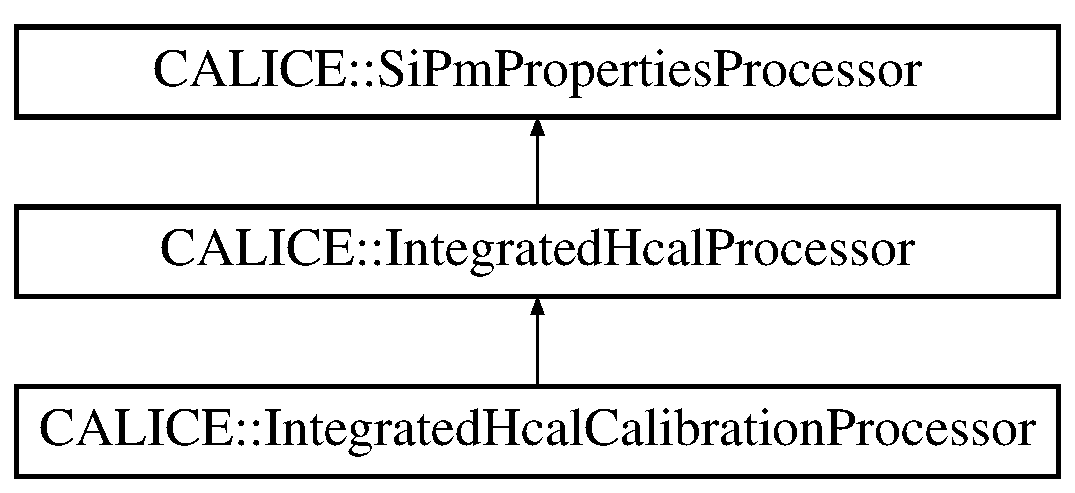
\includegraphics[height=3cm]{classCALICE_1_1SiPmPropertiesProcessor}
\end{center}
\end{figure}
\subsection*{Public Member Functions}
\begin{DoxyCompactItemize}
\item 
{\bf SiPmPropertiesProcessor} $\ast$ {\bfseries newProcessor} ()\label{classCALICE_1_1SiPmPropertiesProcessor_afd454eeb6fff1290816bf47ea42f898c}

\item 
{\bfseries SiPmPropertiesProcessor} (const std::string processorName=\char`\"{}SiPmPropertiesProcessor\char`\"{})\label{classCALICE_1_1SiPmPropertiesProcessor_a044da56a6b19162530ec61e971cfb3aa}

\item 
void {\bfseries init} ()\label{classCALICE_1_1SiPmPropertiesProcessor_a18867a127570598ad26694719ab3c771}

\item 
void {\bfseries processEvent} (LCEvent $\ast$evtP)\label{classCALICE_1_1SiPmPropertiesProcessor_aee931cd7fc7aae6d8cac48383ccf7ddb}

\item 
void {\bfseries processRunHeader} (LCRunHeader $\ast$run)\label{classCALICE_1_1SiPmPropertiesProcessor_aecd18f72518fdf995c5b4f4999f9cc0f}

\item 
bool {\bfseries empty} () const \label{classCALICE_1_1SiPmPropertiesProcessor_a96c5115d41b6e12ac39c9cd0a26f09f7}

\item 
float {\bfseries getSipmVoltage} (const unsigned sipm) const \label{classCALICE_1_1SiPmPropertiesProcessor_a2307382303dd5bb2c08d3295990a4f60}

\item 
float {\bfseries getSipmVoltage} (const unsigned module, const unsigned chip, const unsigned chan) const \label{classCALICE_1_1SiPmPropertiesProcessor_a1de2cff608caca6853e6dd49548cc850}

\item 
float {\bfseries getSipmVoltageBreakdown} (const unsigned sipm) const \label{classCALICE_1_1SiPmPropertiesProcessor_a8a39af189b46542e8d1856c57c5d188c}

\item 
float {\bfseries getSipmVoltageBreakdown} (const unsigned module, const unsigned chip, const unsigned chan) const \label{classCALICE_1_1SiPmPropertiesProcessor_a14383cb4e8ea51d094b7fa26da0ff285}

\item 
float {\bfseries getDelta\_\-SPE} (const unsigned sipm) const \label{classCALICE_1_1SiPmPropertiesProcessor_abfdc56fb42ad7b8bf6e03214bb0b8469}

\item 
float {\bfseries getDelta\_\-SPE} (const unsigned module, const unsigned chip, const unsigned chan) const \label{classCALICE_1_1SiPmPropertiesProcessor_a021746c535440dd242e6b20905de0a1c}

\item 
float {\bfseries getPhe\_\-MIP} (const unsigned sipm) const \label{classCALICE_1_1SiPmPropertiesProcessor_a64772de1f9b49b8ed47fda7d6cc57333}

\item 
float {\bfseries getPhe\_\-MIP} (const unsigned module, const unsigned chip, const unsigned chan) const \label{classCALICE_1_1SiPmPropertiesProcessor_a9db41320e1716882cb33723aa551e836}

\item 
float {\bfseries getTemp} (const unsigned sipm) const \label{classCALICE_1_1SiPmPropertiesProcessor_a91d70d19cf8b218cc0517f334cc07854}

\item 
float {\bfseries getTemp} (const unsigned module, const unsigned chip, const unsigned chan) const \label{classCALICE_1_1SiPmPropertiesProcessor_ad13cd4fa8844c174a70d053ecff3cad1}

\item 
float {\bfseries getCurrent} (const unsigned sipm) const \label{classCALICE_1_1SiPmPropertiesProcessor_a788712be73ed68655e86fd3daed1ec45}

\item 
float {\bfseries getCurrent} (const unsigned module, const unsigned chip, const unsigned chan) const \label{classCALICE_1_1SiPmPropertiesProcessor_ae87066c5331155c15148adc1098afe31}

\item 
float {\bfseries getCurrentRMS} (const unsigned sipm) const \label{classCALICE_1_1SiPmPropertiesProcessor_adcf12d0d6c7817e2f6a606788149695e}

\item 
float {\bfseries getCurrentRMS} (const unsigned module, const unsigned chip, const unsigned chan) const \label{classCALICE_1_1SiPmPropertiesProcessor_ac5701f48c8621fe51e9456f54b7586dc}

\item 
float {\bfseries getDarkRate0} (const unsigned sipm) const \label{classCALICE_1_1SiPmPropertiesProcessor_a83b705eca630fe53acc7e9ccd46f046a}

\item 
float {\bfseries getDarkRate0} (const unsigned module, const unsigned chip, const unsigned chan) const \label{classCALICE_1_1SiPmPropertiesProcessor_a8dda757457c5f5f7be9cbe82a31c611e}

\item 
float {\bfseries getDarkRateHalf} (const unsigned sipm) const \label{classCALICE_1_1SiPmPropertiesProcessor_af67aa9d6cd8306769a804d329092e997}

\item 
float {\bfseries getDarkRateHalf} (const unsigned module, const unsigned chip, const unsigned chan) const \label{classCALICE_1_1SiPmPropertiesProcessor_a51b2b403c16e111b0074849370609d4d}

\item 
float {\bfseries getDarkRateHalfCorr} (const unsigned sipm) const \label{classCALICE_1_1SiPmPropertiesProcessor_ac01a00304f1671020af7089dd869a63c}

\item 
float {\bfseries getDarkRateHalfCorr} (const unsigned module, const unsigned chip, const unsigned chan) const \label{classCALICE_1_1SiPmPropertiesProcessor_afeb80918c3af62a8ea86bd10afb28164}

\item 
float {\bfseries getPedRMS} (const unsigned sipm) const \label{classCALICE_1_1SiPmPropertiesProcessor_a10069f2e761eeab5b2f8a5b46de4a7c1}

\item 
float {\bfseries getPedRMS} (const unsigned module, const unsigned chip, const unsigned chan) const \label{classCALICE_1_1SiPmPropertiesProcessor_abd317d4bf9019e63864b41945a08c5b4}

\item 
float {\bfseries getPeakWidth} (const unsigned sipm) const \label{classCALICE_1_1SiPmPropertiesProcessor_a122927747aaaf7962f73950415e69be2}

\item 
float {\bfseries getPeakWidth} (const unsigned module, const unsigned chip, const unsigned chan) const \label{classCALICE_1_1SiPmPropertiesProcessor_a821960e9dea7268b585c04af86278729}

\item 
float {\bfseries getXTalk} (const unsigned sipm) const \label{classCALICE_1_1SiPmPropertiesProcessor_a49ccb27604b3989489866b70385a9c38}

\item 
float {\bfseries getXTalk} (const unsigned module, const unsigned chip, const unsigned chan) const \label{classCALICE_1_1SiPmPropertiesProcessor_a9a89b6008d0d60bb0b60b6b9d266d236}

\item 
unsigned {\bfseries getSatPointNr} (const unsigned sipm) const \label{classCALICE_1_1SiPmPropertiesProcessor_ad68505357900fde5b0581d213c2e0857}

\item 
unsigned {\bfseries getSatPointNr} (const unsigned module, const unsigned chip, const unsigned chan) const \label{classCALICE_1_1SiPmPropertiesProcessor_aa172924dd56f0c70743c851756e32d74}

\item 
float {\bfseries getSipmPixelSat} (const unsigned sipm, const unsigned point) const \label{classCALICE_1_1SiPmPropertiesProcessor_a1ecb6b6213167728a638f44e2bab3e30}

\item 
float {\bfseries getSipmPixelSat} (const unsigned module, const unsigned chip, const unsigned chan, const unsigned point) const \label{classCALICE_1_1SiPmPropertiesProcessor_a0dcb61b92932aa21ad7d7543fdb00bd8}

\item 
float {\bfseries getPmtMipSat} (const unsigned sipm, const unsigned point) const \label{classCALICE_1_1SiPmPropertiesProcessor_abb586ffb2881f2ff95cd2db60b724de7}

\item 
float {\bfseries getPmtMipSat} (const unsigned module, const unsigned chip, const unsigned chan, const unsigned point) const \label{classCALICE_1_1SiPmPropertiesProcessor_ae144f3314db5a24a359bd0e2f6823a37}

\item 
float {\bfseries getSiPmSaturationCorrection} (const unsigned module, const unsigned chip, const unsigned chan, const float pixel) const \label{classCALICE_1_1SiPmPropertiesProcessor_afd545661631706206e67218f3ef898eb}

\item 
float {\bfseries getSiPmSaturationCorrection} (const unsigned module, const unsigned cell, const float pixel) const \label{classCALICE_1_1SiPmPropertiesProcessor_a8358f97372e0e5d63d95393497420f7f}

\item 
float {\bfseries getInverseSiPmSaturationCorrection} (const unsigned module, const unsigned chip, const unsigned chan, const float pixel) const \label{classCALICE_1_1SiPmPropertiesProcessor_a13dd5628d87e88900168bd676c2426e9}

\item 
float {\bfseries getInverseSiPmSaturationCorrection} (const unsigned module, const unsigned cell, const float pixel) const \label{classCALICE_1_1SiPmPropertiesProcessor_a93644c4c6c78e16498362b7fdde0ddfa}

\item 
unsigned {\bfseries getSipmID} (const unsigned module, const unsigned chip, const unsigned chan) const \label{classCALICE_1_1SiPmPropertiesProcessor_a97b7fa11542d26267b5cd2cc5c0e6a1f}

\item 
unsigned {\bfseries getTileSize} (const unsigned module, const unsigned chip, const unsigned chan) const \label{classCALICE_1_1SiPmPropertiesProcessor_a6b1b49d43a6efbf729f512b863b209fc}

\end{DoxyCompactItemize}
\subsection*{Protected Member Functions}
\begin{DoxyCompactItemize}
\item 
virtual void {\bfseries SipmInfoChanged} (lcio::LCCollection $\ast$col)\label{classCALICE_1_1SiPmPropertiesProcessor_a04285d3e49408159a442ee2d18a055b8}

\item 
virtual void {\bfseries SipmSaturationChanged} (lcio::LCCollection $\ast$col)\label{classCALICE_1_1SiPmPropertiesProcessor_a1f624cf4c071d6b43ec3947bec494d6e}

\item 
virtual void {\bfseries ModuleProductionChanged} (lcio::LCCollection $\ast$col)\label{classCALICE_1_1SiPmPropertiesProcessor_ac5eaa7848cada4dc39deb90cb222146d}

\item 
virtual void {\bfseries pixelScaleFactorsChanged} (lcio::LCCollection $\ast$col)\label{classCALICE_1_1SiPmPropertiesProcessor_a932baad6aff178854e72621ccfa03110}

\item 
virtual void {\bfseries defaultPixelScaleFactorsChanged} (lcio::LCCollection $\ast$col)\label{classCALICE_1_1SiPmPropertiesProcessor_a51b045d2ee4749ce79000a6204653263}

\item 
virtual void {\bfseries UpdateVectors} ()\label{classCALICE_1_1SiPmPropertiesProcessor_aba0a07bc0dbb840965bf3a18f6b0defa}

\end{DoxyCompactItemize}
\subsection*{Protected Attributes}
\begin{DoxyCompactItemize}
\item 
std::string {\bfseries \_\-SiPmInfoColName}\label{classCALICE_1_1SiPmPropertiesProcessor_acb6749fb1dcb670ca6206a0fc5478196}

\item 
std::string {\bfseries \_\-SiPmSaturationColName}\label{classCALICE_1_1SiPmPropertiesProcessor_a66c56f04af769b028268647ddeffe705}

\item 
std::string {\bfseries \_\-ModuleProductionColName}\label{classCALICE_1_1SiPmPropertiesProcessor_a46c6cf33232fba705301d00d02088adc}

\item 
std::string {\bfseries \_\-pixelScaleFactorsColName}\label{classCALICE_1_1SiPmPropertiesProcessor_a2ef504d7d9c26e1303b99de4da217a41}

\item 
std::string {\bfseries \_\-defaultPixelScaleFactorsColName}\label{classCALICE_1_1SiPmPropertiesProcessor_a19a7832e60bdff54a927cbbc53b1cca4}

\item 
int {\bfseries \_\-assumeIncrease}\label{classCALICE_1_1SiPmPropertiesProcessor_a506a0e660344a9b36912b6eae69b6f94}

\item 
int {\bfseries \_\-reduceFluctuations}\label{classCALICE_1_1SiPmPropertiesProcessor_ac5cc7412d5336f3f2e911b2aaf212649}

\item 
float {\bfseries \_\-defaultPixelScaleFactor}\label{classCALICE_1_1SiPmPropertiesProcessor_a90bcbbe027b24839e1968c9b84a555af}

\item 
float {\bfseries \_\-additionalOverallPixelScaleFactor}\label{classCALICE_1_1SiPmPropertiesProcessor_afad2b42ffbb0391e63a263686e6f5f94}

\item 
bool {\bfseries \_\-defaultPixelScaleFactorsEmpty}\label{classCALICE_1_1SiPmPropertiesProcessor_aad80ef59255bbbacf9d31637d642b045}

\item 
lccd::ConditionsMap$<$ int, CALICE::SimpleValue $>$ {\bfseries \_\-defaultPixelScaleFactorsMap}\label{classCALICE_1_1SiPmPropertiesProcessor_ab881fc07e0db31700f84de9a851d4070}

\item 
bool {\bfseries \_\-pixelScaleFactorsEmpty}\label{classCALICE_1_1SiPmPropertiesProcessor_ad0f2dd1b49e6ce68019984f64ca5e994}

\item 
lccd::ConditionsMap$<$ int, CALICE::SimpleValue $>$ {\bfseries \_\-pixelScaleFactorsMap}\label{classCALICE_1_1SiPmPropertiesProcessor_a00f1e01ad1c585c5fa33ff048ad3e17a}

\item 
ConditionsChangeDelegator$<$ {\bf SiPmPropertiesProcessor} $>$ {\bfseries \_\-SiPmInfoChange}\label{classCALICE_1_1SiPmPropertiesProcessor_abfa2958127c2f592a9cf1861bf6f8b8a}

\item 
ConditionsChangeDelegator$<$ {\bf SiPmPropertiesProcessor} $>$ {\bfseries \_\-SiPmSaturationChange}\label{classCALICE_1_1SiPmPropertiesProcessor_afffde1d70dd6fc1d52b50f12c13de3ef}

\item 
ConditionsChangeDelegator$<$ {\bf SiPmPropertiesProcessor} $>$ {\bfseries \_\-ModuleProductionChange}\label{classCALICE_1_1SiPmPropertiesProcessor_a0d2cbe6dab804d78d8eb27a8f3af787f}

\item 
ConditionsChangeDelegator$<$ {\bf SiPmPropertiesProcessor} $>$ {\bfseries \_\-pixelScaleFactorsChange}\label{classCALICE_1_1SiPmPropertiesProcessor_a11a48bdf9a5840d090ef9047b03fcfd4}

\item 
ConditionsChangeDelegator$<$ {\bf SiPmPropertiesProcessor} $>$ {\bfseries \_\-defaultPixelScaleFactorsChange}\label{classCALICE_1_1SiPmPropertiesProcessor_ace4d68c1d75ec060bc60a8ba69014dc1}

\item 
bool {\bfseries \_\-SiPmInfoEmpty}\label{classCALICE_1_1SiPmPropertiesProcessor_adba4eeb5243a0fd5198ab9ffb0979998}

\item 
bool {\bfseries \_\-SiPmSaturationEmpty}\label{classCALICE_1_1SiPmPropertiesProcessor_acb305e30ef61ea06ee84d4188d51aeaf}

\item 
bool {\bfseries \_\-ModuleProductionEmpty}\label{classCALICE_1_1SiPmPropertiesProcessor_a24b9c0152d25707562bca6f25335cbfe}

\item 
std::map$<$ unsigned int, float $>$ {\bfseries \_\-SIPMID\_\-to\_\-scaleFactor}\label{classCALICE_1_1SiPmPropertiesProcessor_ab54d5d21a513778cf3e3f4553f5be538}

\item 
std::map$<$ unsigned, float $>$ {\bfseries \_\-SipmVoltageMap}\label{classCALICE_1_1SiPmPropertiesProcessor_a63365171f3bf33d2134b1897875cba83}

\item 
std::map$<$ unsigned, float $>$ {\bfseries \_\-SipmVoltageBreakdownMap}\label{classCALICE_1_1SiPmPropertiesProcessor_abebd280f89c688a481b501a4510c435b}

\item 
std::map$<$ unsigned, float $>$ {\bfseries \_\-Delta\_\-SPEMap}\label{classCALICE_1_1SiPmPropertiesProcessor_a2b53b09013432289bbf15a422b10b599}

\item 
std::map$<$ unsigned, float $>$ {\bfseries \_\-Phe\_\-MIPMap}\label{classCALICE_1_1SiPmPropertiesProcessor_a587b49d56165a88a3938f7fd26b82110}

\item 
std::map$<$ unsigned, float $>$ {\bfseries \_\-TempMap}\label{classCALICE_1_1SiPmPropertiesProcessor_af04cc739127d761f2b1ae305b574cdb3}

\item 
std::map$<$ unsigned, float $>$ {\bfseries \_\-CurrentMap}\label{classCALICE_1_1SiPmPropertiesProcessor_a3481e547f6872a3b8c61f81f79dd2a57}

\item 
std::map$<$ unsigned, float $>$ {\bfseries \_\-CurrentRMSMap}\label{classCALICE_1_1SiPmPropertiesProcessor_a6650a16201f45447c8f0e1187747ab6a}

\item 
std::map$<$ unsigned, float $>$ {\bfseries \_\-DarkRate0Map}\label{classCALICE_1_1SiPmPropertiesProcessor_a6cb7ed611c785639effe2b6d776fde93}

\item 
std::map$<$ unsigned, float $>$ {\bfseries \_\-DarkRateHalfMap}\label{classCALICE_1_1SiPmPropertiesProcessor_ad8580b0ff0a779571753ae4e7312bad5}

\item 
std::map$<$ unsigned, float $>$ {\bfseries \_\-DarkRateHalfCorrMap}\label{classCALICE_1_1SiPmPropertiesProcessor_a87fcb0172fd11803f6df6d98d4263481}

\item 
std::map$<$ unsigned, float $>$ {\bfseries \_\-PedRMSMap}\label{classCALICE_1_1SiPmPropertiesProcessor_a6a9b968b7530a1395cce90166158ffdb}

\item 
std::map$<$ unsigned, float $>$ {\bfseries \_\-PeakWidthMap}\label{classCALICE_1_1SiPmPropertiesProcessor_aa7a3db0ca5b0c1814fdc1dfdc8a4b69f}

\item 
std::map$<$ unsigned, float $>$ {\bfseries \_\-XTalkMap}\label{classCALICE_1_1SiPmPropertiesProcessor_a38d20696ef1e2cb20b0bf86f2351b0d8}

\item 
std::vector$<$ float $>$ {\bfseries \_\-SipmVoltageVector}\label{classCALICE_1_1SiPmPropertiesProcessor_ac8b3a5950031ca74ab882c224042e451}

\item 
std::vector$<$ float $>$ {\bfseries \_\-SipmVoltageBreakdownVector}\label{classCALICE_1_1SiPmPropertiesProcessor_a633aa5eb479e59866e21f038d1428dad}

\item 
std::vector$<$ float $>$ {\bfseries \_\-Delta\_\-SPEVector}\label{classCALICE_1_1SiPmPropertiesProcessor_a59e24efe83279c1ad2d35f4a0ff47978}

\item 
std::vector$<$ float $>$ {\bfseries \_\-Phe\_\-MIPVector}\label{classCALICE_1_1SiPmPropertiesProcessor_a8735696ed23d99a31fe78b9458ca6ea4}

\item 
std::vector$<$ float $>$ {\bfseries \_\-TempVector}\label{classCALICE_1_1SiPmPropertiesProcessor_a062963e5878e6510f5e05ed477f0d7b5}

\item 
std::vector$<$ float $>$ {\bfseries \_\-CurrentVector}\label{classCALICE_1_1SiPmPropertiesProcessor_ac4b06cb71b779bc05186055e15e4d76b}

\item 
std::vector$<$ float $>$ {\bfseries \_\-CurrentRMSVector}\label{classCALICE_1_1SiPmPropertiesProcessor_a048c286afd43ffe74a8a00f17ab1052b}

\item 
std::vector$<$ float $>$ {\bfseries \_\-DarkRate0Vector}\label{classCALICE_1_1SiPmPropertiesProcessor_a9f1349bd2083fc0c83a637e3fec5cbe9}

\item 
std::vector$<$ float $>$ {\bfseries \_\-DarkRateHalfVector}\label{classCALICE_1_1SiPmPropertiesProcessor_a4e424b5ebbb1f20d053d3865be63f53e}

\item 
std::vector$<$ float $>$ {\bfseries \_\-DarkRateHalfCorrVector}\label{classCALICE_1_1SiPmPropertiesProcessor_a6111cc7e9b04e0855f48b4ec5b758190}

\item 
std::vector$<$ float $>$ {\bfseries \_\-PedRMSVector}\label{classCALICE_1_1SiPmPropertiesProcessor_abc8201a9b8ebbfd0943863c3ea44d988}

\item 
std::vector$<$ float $>$ {\bfseries \_\-PeakWidthVector}\label{classCALICE_1_1SiPmPropertiesProcessor_ac51ad1f3b42c8d4e6ed22a578cab93e1}

\item 
std::vector$<$ float $>$ {\bfseries \_\-XTalkVector}\label{classCALICE_1_1SiPmPropertiesProcessor_aaed7eb60832cf27397c07d29f02b3655}

\item 
std::map$<$ unsigned, float $>$ {\bfseries \_\-SipmPixelSatMap} [SATPOINTS]\label{classCALICE_1_1SiPmPropertiesProcessor_aac2e9c79a36b6b8a2142f90a43d49ac0}

\item 
std::map$<$ unsigned, float $>$ {\bfseries \_\-PmtMipSatMap} [SATPOINTS]\label{classCALICE_1_1SiPmPropertiesProcessor_af66eeb8207a9f06138ebdd3691ca87b3}

\item 
std::vector$<$ float $>$ {\bfseries \_\-SipmPixelSatVector} [SATPOINTS]\label{classCALICE_1_1SiPmPropertiesProcessor_a7ffbe1262a0e69b16409c0a0b6f6d7dc}

\item 
std::vector$<$ float $>$ {\bfseries \_\-PmtMipSatVector} [SATPOINTS]\label{classCALICE_1_1SiPmPropertiesProcessor_ab16b4671505857cddbd7bed4e0976677}

\item 
std::vector$<$ float $>$ {\bfseries \_\-InterpolationA} [SATPOINTS]\label{classCALICE_1_1SiPmPropertiesProcessor_acba8a855860b9dcf60e7d2af825f6ffb}

\item 
std::vector$<$ float $>$ {\bfseries \_\-InterpolationB} [SATPOINTS]\label{classCALICE_1_1SiPmPropertiesProcessor_a6140eb844de35c9d12005f07ca703bf2}

\item 
std::map$<$ unsigned, unsigned $>$ {\bfseries \_\-SIPMMap}\label{classCALICE_1_1SiPmPropertiesProcessor_a74ce5786f56b407136f1296c52186217}

\item 
std::map$<$ unsigned, unsigned $>$ {\bfseries \_\-TileSizeMap}\label{classCALICE_1_1SiPmPropertiesProcessor_a2809f9f20605f6b9e45413fdd366acc8}

\item 
std::vector$<$ unsigned $>$ {\bfseries \_\-SIPMVector}\label{classCALICE_1_1SiPmPropertiesProcessor_a4b3c0339d341c2644acd956c3c94ae30}

\item 
std::vector$<$ unsigned $>$ {\bfseries \_\-TileSizeVector}\label{classCALICE_1_1SiPmPropertiesProcessor_ae794aaa1cbba31e6b41928f2c39c2110}

\item 
std::vector$<$ TGraph $\ast$ $>$ {\bfseries \_\-corGraphVector}\label{classCALICE_1_1SiPmPropertiesProcessor_a05341072000f27ed32a970efa463dfaf}

\item 
std::vector$<$ TGraph $\ast$ $>$ {\bfseries \_\-satGraphVector}\label{classCALICE_1_1SiPmPropertiesProcessor_ac6fda8c85d1d6883fa424c7d19c26b1c}

\end{DoxyCompactItemize}


\subsection{Detailed Description}


Definition at line 28 of file SiPmPropertiesProcessor.hh.

The documentation for this class was generated from the following files:\begin{DoxyCompactItemize}
\item 
SiPmPropertiesProcessor.hh\item 
SiPmPropertiesProcessor.cc\end{DoxyCompactItemize}

\section{CALICE::SquareFinder Class Reference}
\label{classCALICE_1_1SquareFinder}\index{CALICE::SquareFinder@{CALICE::SquareFinder}}


Processor to search for events where the whole border of a wafer is firing.  


{\ttfamily \#include $<$SquareFinder.hh$>$}\subsection*{Public Member Functions}
\begin{DoxyCompactItemize}
\item 
Processor $\ast$ {\bfseries newProcessor} ()\label{classCALICE_1_1SquareFinder_a3f2f49aba9c7f0d76d62de5a6c9e5ee1}

\item 
{\bf SquareFinder} ()
\begin{DoxyCompactList}\small\item\em Select Mips . \item\end{DoxyCompactList}\item 
void {\bf init} ()
\begin{DoxyCompactList}\small\item\em Called at the begin of the job before anything is read. \item\end{DoxyCompactList}\item 
void {\bf processRunHeader} (LCRunHeader $\ast$run)
\begin{DoxyCompactList}\small\item\em Called for every run, e.g. \item\end{DoxyCompactList}\item 
void {\bf processEvent} (LCEvent $\ast$evtP)\label{classCALICE_1_1SquareFinder_ac15ccd383747f853c1480d687f9dba7f}

\begin{DoxyCompactList}\small\item\em Called for every event -\/ the working horse. \item\end{DoxyCompactList}\item 
void {\bfseries end} ()\label{classCALICE_1_1SquareFinder_a93abe832b780c7ce5616ca29d16c72ac}

\end{DoxyCompactItemize}
\subsection*{Protected Attributes}
\begin{DoxyCompactItemize}
\item 
Int\_\-t {\bf \_\-nHitsMin}\label{classCALICE_1_1SquareFinder_a2c9c17a9f50875e1762b5c2347209d3c}

\begin{DoxyCompactList}\small\item\em minimum number of hits on the border of the wafer \item\end{DoxyCompactList}\item 
Int\_\-t {\bf \_\-nInsidedHitsMax}
\begin{DoxyCompactList}\small\item\em maximum number of hits inside the wafer. \item\end{DoxyCompactList}\item 
std::string {\bf \_\-colName}
\begin{DoxyCompactList}\small\item\em name of the hit input collection (Marlin processor parameter). \item\end{DoxyCompactList}\item 
std::string {\bf \_\-clusterColName}
\begin{DoxyCompactList}\small\item\em name of the square cluster collection. \item\end{DoxyCompactList}\item 
std::string {\bf \_\-squareFlagName}
\begin{DoxyCompactList}\small\item\em name of the event parameter which flags square events. \item\end{DoxyCompactList}\item 
FloatVec {\bf \_\-signalHistPar}
\begin{DoxyCompactList}\small\item\em binning of the border and total border signal histograms. \item\end{DoxyCompactList}\item 
UInt\_\-t {\bf \_\-nSquareEvents}
\begin{DoxyCompactList}\small\item\em Number of square event candidates. \item\end{DoxyCompactList}\item 
UInt\_\-t {\bf \_\-nEvents}
\begin{DoxyCompactList}\small\item\em Total number of events with hits. \item\end{DoxyCompactList}\end{DoxyCompactItemize}


\subsection{Detailed Description}
Processor to search for events where the whole border of a wafer is firing. 

Definition at line 27 of file SquareFinder.hh.

\subsection{Constructor \& Destructor Documentation}
\index{CALICE::SquareFinder@{CALICE::SquareFinder}!SquareFinder@{SquareFinder}}
\index{SquareFinder@{SquareFinder}!CALICE::SquareFinder@{CALICE::SquareFinder}}
\subsubsection[{SquareFinder}]{\setlength{\rightskip}{0pt plus 5cm}CALICE::SquareFinder::SquareFinder ()}\label{classCALICE_1_1SquareFinder_a048810eab2155fd081f4ce775c49ff11}


Select Mips . Mip tracks are search within the calorimeter hits. Developped for cosmics. 

Definition at line 44 of file SquareFinder.cc.

References \_\-clusterColName, \_\-colName, \_\-nHitsMin, \_\-nInsidedHitsMax, \_\-signalHistPar, and \_\-squareFlagName.

\subsection{Member Function Documentation}
\index{CALICE::SquareFinder@{CALICE::SquareFinder}!init@{init}}
\index{init@{init}!CALICE::SquareFinder@{CALICE::SquareFinder}}
\subsubsection[{init}]{\setlength{\rightskip}{0pt plus 5cm}void CALICE::SquareFinder::init ()}\label{classCALICE_1_1SquareFinder_aebcf72e750bcecb0304266a9a5449dba}


Called at the begin of the job before anything is read. Use to initialize the processor, e.g. book histograms. 

Definition at line 112 of file SquareFinder.cc.

References \_\-clusterColName, \_\-nEvents, \_\-nSquareEvents, \_\-signalHistPar, histmgr::HistMgr::create2DHistograms(), and histmgr::HistMgr::createHistograms().\index{CALICE::SquareFinder@{CALICE::SquareFinder}!processRunHeader@{processRunHeader}}
\index{processRunHeader@{processRunHeader}!CALICE::SquareFinder@{CALICE::SquareFinder}}
\subsubsection[{processRunHeader}]{\setlength{\rightskip}{0pt plus 5cm}void CALICE::SquareFinder::processRunHeader (LCRunHeader $\ast$ {\em run})\hspace{0.3cm}{\ttfamily  [inline]}}\label{classCALICE_1_1SquareFinder_a876db4e7ce9e481a7bba79a5c543372f}


Called for every run, e.g. overwrite to initialize run dependent histograms. 

Definition at line 45 of file SquareFinder.hh.

\subsection{Field Documentation}
\index{CALICE::SquareFinder@{CALICE::SquareFinder}!\_\-clusterColName@{\_\-clusterColName}}
\index{\_\-clusterColName@{\_\-clusterColName}!CALICE::SquareFinder@{CALICE::SquareFinder}}
\subsubsection[{\_\-clusterColName}]{\setlength{\rightskip}{0pt plus 5cm}std::string {\bf CALICE::SquareFinder::\_\-clusterColName}\hspace{0.3cm}{\ttfamily  [protected]}}\label{classCALICE_1_1SquareFinder_ad92613a91542bc47728aa0b37b46ea09}


name of the square cluster collection. 

Definition at line 57 of file SquareFinder.hh.

Referenced by init(), processEvent(), and SquareFinder().\index{CALICE::SquareFinder@{CALICE::SquareFinder}!\_\-colName@{\_\-colName}}
\index{\_\-colName@{\_\-colName}!CALICE::SquareFinder@{CALICE::SquareFinder}}
\subsubsection[{\_\-colName}]{\setlength{\rightskip}{0pt plus 5cm}std::string {\bf CALICE::SquareFinder::\_\-colName}\hspace{0.3cm}{\ttfamily  [protected]}}\label{classCALICE_1_1SquareFinder_a8f394987f130f4e495032fd256257ac0}


name of the hit input collection (Marlin processor parameter). 

Definition at line 56 of file SquareFinder.hh.

Referenced by processEvent(), and SquareFinder().\index{CALICE::SquareFinder@{CALICE::SquareFinder}!\_\-nEvents@{\_\-nEvents}}
\index{\_\-nEvents@{\_\-nEvents}!CALICE::SquareFinder@{CALICE::SquareFinder}}
\subsubsection[{\_\-nEvents}]{\setlength{\rightskip}{0pt plus 5cm}UInt\_\-t {\bf CALICE::SquareFinder::\_\-nEvents}\hspace{0.3cm}{\ttfamily  [protected]}}\label{classCALICE_1_1SquareFinder_a5110e34b92e02a21bf870ff104e59745}


Total number of events with hits. 

Definition at line 62 of file SquareFinder.hh.

Referenced by init(), and processEvent().\index{CALICE::SquareFinder@{CALICE::SquareFinder}!\_\-nInsidedHitsMax@{\_\-nInsidedHitsMax}}
\index{\_\-nInsidedHitsMax@{\_\-nInsidedHitsMax}!CALICE::SquareFinder@{CALICE::SquareFinder}}
\subsubsection[{\_\-nInsidedHitsMax}]{\setlength{\rightskip}{0pt plus 5cm}Int\_\-t {\bf CALICE::SquareFinder::\_\-nInsidedHitsMax}\hspace{0.3cm}{\ttfamily  [protected]}}\label{classCALICE_1_1SquareFinder_ab81ff4d872972c06c2d072c9e681b321}


maximum number of hits inside the wafer. 

Definition at line 55 of file SquareFinder.hh.

Referenced by processEvent(), and SquareFinder().\index{CALICE::SquareFinder@{CALICE::SquareFinder}!\_\-nSquareEvents@{\_\-nSquareEvents}}
\index{\_\-nSquareEvents@{\_\-nSquareEvents}!CALICE::SquareFinder@{CALICE::SquareFinder}}
\subsubsection[{\_\-nSquareEvents}]{\setlength{\rightskip}{0pt plus 5cm}UInt\_\-t {\bf CALICE::SquareFinder::\_\-nSquareEvents}\hspace{0.3cm}{\ttfamily  [protected]}}\label{classCALICE_1_1SquareFinder_a85c4e30fac259f17c8bbcb789b28d871}


Number of square event candidates. 

Definition at line 61 of file SquareFinder.hh.

Referenced by init(), and processEvent().\index{CALICE::SquareFinder@{CALICE::SquareFinder}!\_\-signalHistPar@{\_\-signalHistPar}}
\index{\_\-signalHistPar@{\_\-signalHistPar}!CALICE::SquareFinder@{CALICE::SquareFinder}}
\subsubsection[{\_\-signalHistPar}]{\setlength{\rightskip}{0pt plus 5cm}FloatVec {\bf CALICE::SquareFinder::\_\-signalHistPar}\hspace{0.3cm}{\ttfamily  [protected]}}\label{classCALICE_1_1SquareFinder_ad1db2cd08984b84ab549c2631b2e679d}


binning of the border and total border signal histograms. 

Definition at line 59 of file SquareFinder.hh.

Referenced by init(), and SquareFinder().\index{CALICE::SquareFinder@{CALICE::SquareFinder}!\_\-squareFlagName@{\_\-squareFlagName}}
\index{\_\-squareFlagName@{\_\-squareFlagName}!CALICE::SquareFinder@{CALICE::SquareFinder}}
\subsubsection[{\_\-squareFlagName}]{\setlength{\rightskip}{0pt plus 5cm}std::string {\bf CALICE::SquareFinder::\_\-squareFlagName}\hspace{0.3cm}{\ttfamily  [protected]}}\label{classCALICE_1_1SquareFinder_a559678746ea01e5a0b4dc1c09901493d}


name of the event parameter which flags square events. 

Definition at line 58 of file SquareFinder.hh.

Referenced by processEvent(), and SquareFinder().

The documentation for this class was generated from the following files:\begin{DoxyCompactItemize}
\item 
SquareFinder.hh\item 
SquareFinder.cc\end{DoxyCompactItemize}

\section{CALICE::Stat\_\-t Class Reference}
\label{classCALICE_1_1Stat__t}\index{CALICE::Stat\_\-t@{CALICE::Stat\_\-t}}


Caclulate mean and RMS vaslue of a set of input values.  


{\ttfamily \#include $<$Box.hh$>$}\subsection*{Public Member Functions}
\begin{DoxyCompactItemize}
\item 
void {\bfseries reset} ()\label{classCALICE_1_1Stat__t_acf6555a00a6567e5f3bd64b286147105}

\item 
void {\bfseries add} (Float\_\-t value, Float\_\-t weight=1.)\label{classCALICE_1_1Stat__t_a7b345a82593acd04ae8ec24093e60e3b}

\item 
void {\bfseries calculate} ()\label{classCALICE_1_1Stat__t_a3e81369ea9d0f2603dad3a3bb6d20209}

\item 
Double\_\-t {\bfseries mean} () const \label{classCALICE_1_1Stat__t_a324b40b1f06f41039dd0a9d72055f31e}

\item 
Double\_\-t {\bfseries sigma} () const \label{classCALICE_1_1Stat__t_a9a287b6c964273a4d2b246de7a99d7c5}

\end{DoxyCompactItemize}
\subsection*{Protected Attributes}
\begin{DoxyCompactItemize}
\item 
Double\_\-t {\bfseries \_\-weight}\label{classCALICE_1_1Stat__t_a770e755b2931194f594656e1e5cb7834}

\item 
Double\_\-t {\bfseries \_\-sum}\label{classCALICE_1_1Stat__t_af46eefdce2686e0d5d94fe9361a404df}

\item 
Double\_\-t {\bfseries \_\-mean}\label{classCALICE_1_1Stat__t_a4793d99948d5879898302766cfa1f122}

\item 
Double\_\-t {\bfseries \_\-sum2}\label{classCALICE_1_1Stat__t_a9940d9384886fc045c90457759225bbc}

\item 
Double\_\-t {\bfseries \_\-sigma}\label{classCALICE_1_1Stat__t_a2594c72a5f89186db65cf86195edec43}

\end{DoxyCompactItemize}
\subsection*{Friends}
\begin{DoxyCompactItemize}
\item 
std::ostream \& {\bfseries operator$<$$<$} (std::ostream \&os, {\bf Stat\_\-t} \&a)\label{classCALICE_1_1Stat__t_a33122c0e8d33292956fdbf1d86680205}

\end{DoxyCompactItemize}


\subsection{Detailed Description}
Caclulate mean and RMS vaslue of a set of input values. 

Definition at line 12 of file Box.hh.

The documentation for this class was generated from the following file:\begin{DoxyCompactItemize}
\item 
Box.hh\end{DoxyCompactItemize}

\section{TBTrackScatter::TBEvent Class Reference}
\label{classTBTrackScatter_1_1TBEvent}\index{TBTrackScatter::TBEvent@{TBTrackScatter::TBEvent}}
\subsection*{Data Fields}
\begin{DoxyCompactItemize}
\item 
double {\bfseries hitPos} [2][NLAYER]\label{classTBTrackScatter_1_1TBEvent_a52e8168b36764a718e4fe6c0ad132951}

\item 
double {\bfseries mcProdPos} [2]\label{classTBTrackScatter_1_1TBEvent_acb19b8e5107a14348b0900faf9de9037}

\item 
double {\bfseries fakePos} [2]\label{classTBTrackScatter_1_1TBEvent_ad2224c9b948a99a94923b57b71e709b3}

\item 
double {\bfseries hitDir} [2][NLAYER]\label{classTBTrackScatter_1_1TBEvent_ae11e105e2f208225844097be44c2209f}

\item 
double {\bfseries mcProdDir} [2]\label{classTBTrackScatter_1_1TBEvent_a6b0ad06b6859dfa4d3b33ce6ceab37ed}

\item 
double {\bfseries fakeDir} [2]\label{classTBTrackScatter_1_1TBEvent_ab9a7089d86050e755f701ca3c9a530ad}

\item 
double {\bfseries fakeExtrapPos} [2][NLAYER]\label{classTBTrackScatter_1_1TBEvent_aead73b11610a89b2bec00b298d2c4a54}

\item 
double {\bfseries mcExtrapPos} [2][NLAYER]\label{classTBTrackScatter_1_1TBEvent_a51446ed1379b77dd2bda8d177886fede}

\end{DoxyCompactItemize}


\subsection{Detailed Description}


Definition at line 63 of file TBTrackScatter.hh.

The documentation for this class was generated from the following file:\begin{DoxyCompactItemize}
\item 
TBTrackScatter.hh\end{DoxyCompactItemize}

\section{TBTrackAligner Class Reference}
\label{classTBTrackAligner}\index{TBTrackAligner@{TBTrackAligner}}
Inheritance diagram for TBTrackAligner::\begin{figure}[H]
\begin{center}
\leavevmode
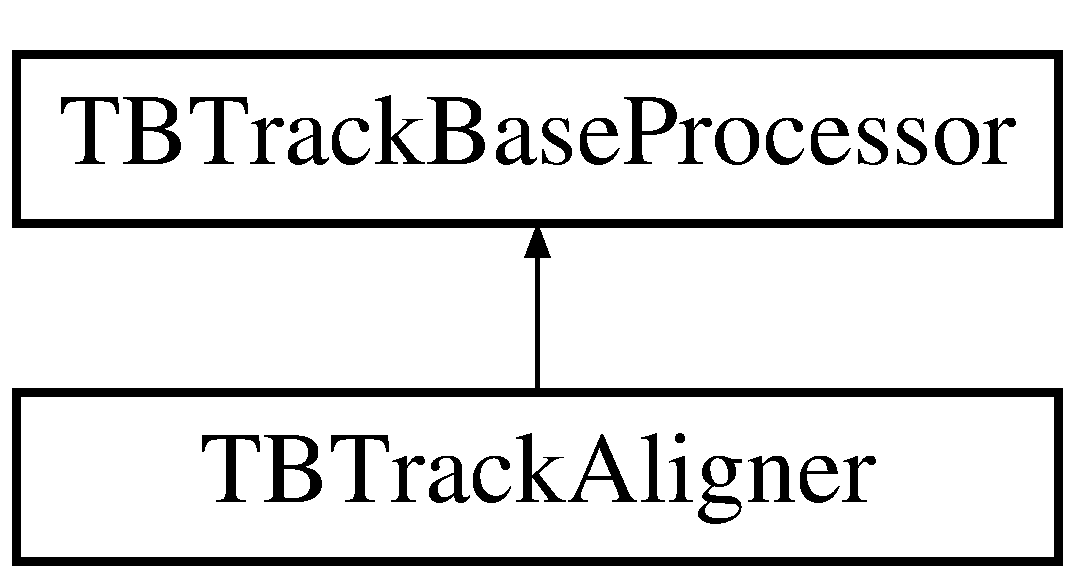
\includegraphics[height=2cm]{classTBTrackAligner}
\end{center}
\end{figure}
\subsection*{Data Structures}
\begin{DoxyCompactItemize}
\item 
class {\bf EventHits}
\begin{DoxyCompactList}\small\item\em Method to write the histograms in a ROOT file. \item\end{DoxyCompactList}\end{DoxyCompactItemize}
\subsection*{Public Member Functions}
\begin{DoxyCompactItemize}
\item 
virtual Processor $\ast$ {\bfseries newProcessor} ()\label{classTBTrackAligner_ab27cfabdbaac3f2f51abc8be398b0c3e}

\item 
virtual void {\bf Init} ()
\begin{DoxyCompactList}\small\item\em Called at the begin of the job before anything is read. \item\end{DoxyCompactList}\item 
virtual void {\bfseries initHists} (unsigned p, bool t)\label{classTBTrackAligner_a57dd9a9703c4733f868294e6e93897cc}

\item 
virtual void {\bf ProcessRunHeader} (LCRunHeader $\ast$run)\label{classTBTrackAligner_a0ac4e729acb1e02c52f6ece3bc8b8b47}

\begin{DoxyCompactList}\small\item\em Called for every run. \item\end{DoxyCompactList}\item 
virtual void {\bf ProcessEvent} (LCEvent $\ast$evt)\label{classTBTrackAligner_a496379cef405a24bc80d8ec7a70686fb}

\begin{DoxyCompactList}\small\item\em Called for every event -\/ the working horse. \item\end{DoxyCompactList}\item 
virtual void {\bf End} ()\label{classTBTrackAligner_a6070161df8594c662cb572b8f4edd93a}

\begin{DoxyCompactList}\small\item\em Called after data processing for clean up. \item\end{DoxyCompactList}\end{DoxyCompactItemize}
\subsection*{Private Attributes}
\begin{DoxyCompactItemize}
\item 
unsigned {\bfseries \_\-highProb} [2][17]\label{classTBTrackAligner_a84b06cd379973894683c4ff5149184dd}

\item 
std::vector$<$ {\bf EventHits} $>$ {\bfseries \_\-vEventHits}\label{classTBTrackAligner_a5c6ddddba21085e33d42b11e2d422bfc}

\item 
TH1F $\ast$ {\bfseries hNumb} [2][17]\label{classTBTrackAligner_ad3bc07a2152a746a4c9b0421ca9726db}

\item 
TH1F $\ast$ {\bfseries hPatt} [2][17]\label{classTBTrackAligner_ac4e1e6d6e4713df266dad1dcb1d21ee0}

\item 
TH1F $\ast$ {\bfseries hPar0} [2][17]\label{classTBTrackAligner_a9f650a0b52fc7310e40f585528ae4493}

\item 
TH1F $\ast$ {\bfseries hPar1} [2][17]\label{classTBTrackAligner_a5e2a1d7b0ccf41fbc7688dd30f3c8a8e}

\item 
TH1F $\ast$ {\bfseries hErr0} [2][17]\label{classTBTrackAligner_a01fc9327217160b2156e70bdb92aff42}

\item 
TH1F $\ast$ {\bfseries hErr1} [2][17]\label{classTBTrackAligner_ac65bf51d7bd36288095648af52fa1f1d}

\item 
TH1F $\ast$ {\bfseries hCorr} [2][17]\label{classTBTrackAligner_a73a3c754d6cad7cbd808eb5eb774af3c}

\item 
TH1F $\ast$ {\bfseries hProb} [2][17]\label{classTBTrackAligner_a210d71981fd2c6458373af716c51be86}

\item 
TH2F $\ast$ {\bfseries hNmb2} [2][17]\label{classTBTrackAligner_aa9da39c486f6eca63b73f4493dde371a}

\item 
TH2F $\ast$ {\bfseries hPrb2} [2][17]\label{classTBTrackAligner_adb4cdb6ce68506ed205d38ad5e6fbf7f}

\item 
TH1F $\ast$ {\bfseries hMPr0} [2][17]\label{classTBTrackAligner_ad830dd1d1bb766c9c311096c8af640c8}

\item 
TH1F $\ast$ {\bfseries hMPr1} [2][17]\label{classTBTrackAligner_abe3da835695654538e6dfdf8d23beecb}

\item 
TH1F $\ast$ {\bfseries hMDf0} [2][17]\label{classTBTrackAligner_a7eb3cf9ed18f91e44e53bb325033177d}

\item 
TH1F $\ast$ {\bfseries hMDf1} [2][17]\label{classTBTrackAligner_a9721cba8515c2270ef25a52eef0b764d}

\end{DoxyCompactItemize}


\subsection{Detailed Description}


Definition at line 17 of file TBTrackAligner.hh.

\subsection{Member Function Documentation}
\index{TBTrackAligner@{TBTrackAligner}!Init@{Init}}
\index{Init@{Init}!TBTrackAligner@{TBTrackAligner}}
\subsubsection[{Init}]{\setlength{\rightskip}{0pt plus 5cm}void TBTrackAligner::Init ()\hspace{0.3cm}{\ttfamily  [virtual]}}\label{classTBTrackAligner_a0f999c70adb52bcb8ce25f517b5b0f70}


Called at the begin of the job before anything is read. Use to initialize the processor, e.g. book histograms. 

Implements {\bf TBTrackBaseProcessor} \doxyref{}{p.}{classTBTrackBaseProcessor}.

Definition at line 94 of file TBTrackAligner.cc.

The documentation for this class was generated from the following files:\begin{DoxyCompactItemize}
\item 
TBTrackAligner.hh\item 
TBTrackAligner.cc\end{DoxyCompactItemize}

\section{TBTrackBaseProcessor Class Reference}
\label{classTBTrackBaseProcessor}\index{TBTrackBaseProcessor@{TBTrackBaseProcessor}}
Inheritance diagram for TBTrackBaseProcessor::\begin{figure}[H]
\begin{center}
\leavevmode
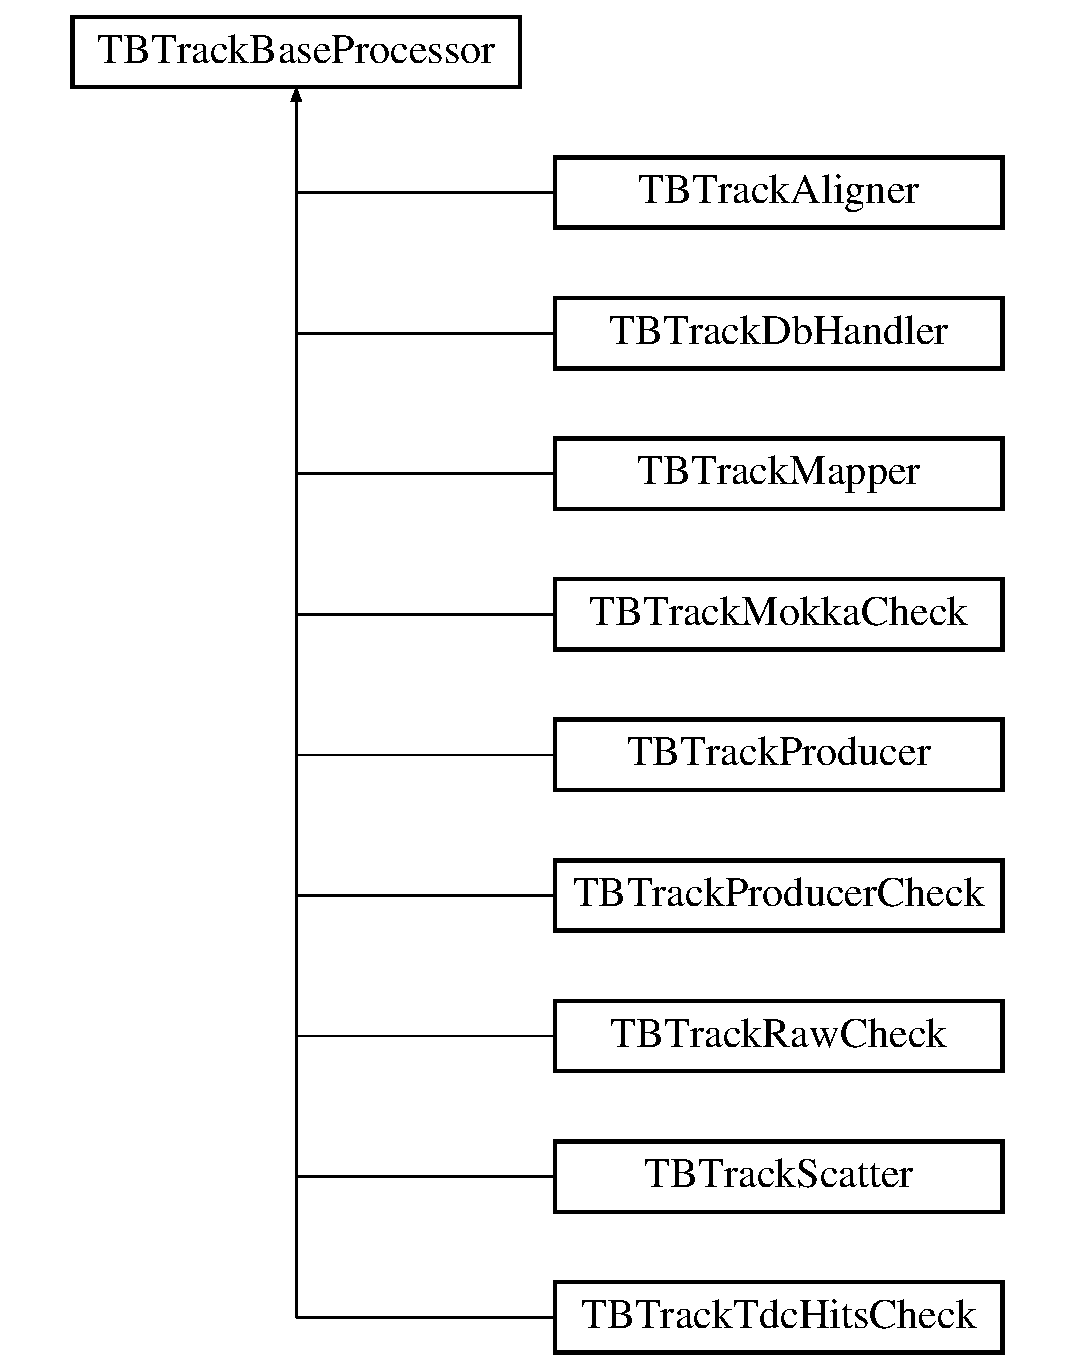
\includegraphics[height=10cm]{classTBTrackBaseProcessor}
\end{center}
\end{figure}
\subsection*{Public Member Functions}
\begin{DoxyCompactItemize}
\item 
{\bfseries TBTrackBaseProcessor} (const std::string \&n=\char`\"{}TBTrackBaseProcessor\char`\"{})\label{classTBTrackBaseProcessor_a8e2072bc1fffd5cdf065b13e865733a0}

\item 
virtual void {\bf init} ()\label{classTBTrackBaseProcessor_a179b559dd67f1777b0622775918ae5f5}

\begin{DoxyCompactList}\small\item\em Called at the begin of the job before anything is read. \item\end{DoxyCompactList}\item 
virtual void {\bfseries Init} ()=0\label{classTBTrackBaseProcessor_a3efab6d4a570bdb0d0059105adef62fb}

\item 
virtual void {\bf processRunHeader} (EVENT::LCRunHeader $\ast$run)\label{classTBTrackBaseProcessor_a0fc18422f19b4c46ec4356df49b216c9}

\begin{DoxyCompactList}\small\item\em Called for every run. \item\end{DoxyCompactList}\item 
virtual void {\bfseries ProcessRunHeader} (EVENT::LCRunHeader $\ast$run)=0\label{classTBTrackBaseProcessor_a644859097b4910c8c6f8c8113bfee2c6}

\item 
virtual void {\bf processEvent} (EVENT::LCEvent $\ast$evt)\label{classTBTrackBaseProcessor_aba4e5b25679936687667e81f3a73df72}

\begin{DoxyCompactList}\small\item\em Called for every event. \item\end{DoxyCompactList}\item 
virtual void {\bfseries ProcessEvent} (EVENT::LCEvent $\ast$evt)=0\label{classTBTrackBaseProcessor_af0b02579767b903b46f9e220efcb83cc}

\item 
virtual void {\bf check} (EVENT::LCEvent $\ast$evt)\label{classTBTrackBaseProcessor_acdf5ee99137016fe8cc9681c0336fc85}

\begin{DoxyCompactList}\small\item\em Called for every event for checking. \item\end{DoxyCompactList}\item 
virtual void {\bf end} ()\label{classTBTrackBaseProcessor_aafbf0e1c1af756ea03748e482883d763}

\begin{DoxyCompactList}\small\item\em Called after data processing for clean up. \item\end{DoxyCompactList}\item 
virtual void {\bfseries End} ()=0\label{classTBTrackBaseProcessor_a5103e722aff198e1a86efb76ffb753ae}

\end{DoxyCompactItemize}
\subsection*{Protected Member Functions}
\begin{DoxyCompactItemize}
\item 
virtual bool {\bf printLevel} (int p, bool b=true) const \label{classTBTrackBaseProcessor_ad49019aae6d63f24ddac47796645beb4}

\begin{DoxyCompactList}\small\item\em Useful methods. \item\end{DoxyCompactList}\item 
virtual void {\bfseries getEvtConstants} (const EVENT::LCEvent $\ast$evt)\label{classTBTrackBaseProcessor_ab7f028108220f667f0771c62b50284a7}

\item 
virtual const EVENT::LCCollection $\ast$ {\bfseries getCollection} (const EVENT::LCEvent $\ast$evt, const std::string \&name, const std::string \&type, bool allowPrint=true) const \label{classTBTrackBaseProcessor_a7d6672702b9966e1aa85b277ccb65c1e}

\item 
virtual bool {\bfseries addCollection} (EVENT::LCEvent $\ast$evt, EVENT::LCCollection $\ast$c, const std::string \&name, bool allowPrint=true) const \label{classTBTrackBaseProcessor_a8c506fe8b1a3854dc18729e8c3253f16}

\item 
void {\bfseries openHFile} (const EVENT::LCRunHeader $\ast$run)\label{classTBTrackBaseProcessor_ae88273f99fda5f6a3bcf94b16bcf96c9}

\item 
void {\bfseries closeHFile} ()\label{classTBTrackBaseProcessor_a258362bb0b7dd5126d069cc0bfcda956}

\item 
void {\bfseries getSimTrackerHits} (EVENT::LCEvent $\ast$evt)\label{classTBTrackBaseProcessor_aff9e06323f04642534a8522ea255497d}

\end{DoxyCompactItemize}
\subsection*{Protected Attributes}
\begin{DoxyCompactItemize}
\item 
{\bf TBTrack::MapConstants} {\bf \_\-mapConstants}\label{classTBTrackBaseProcessor_aa3c3920945b6b96403927e68a4f2d597}

\begin{DoxyCompactList}\small\item\em The database information objects. \item\end{DoxyCompactList}\item 
bool {\bfseries \_\-mapConstantsUpdated}\label{classTBTrackBaseProcessor_ac2ee432d8acdab0d231ae0b58f5d6e4b}

\item 
bool {\bfseries \_\-mapConstantsValid}\label{classTBTrackBaseProcessor_ad88c3ed8dec6a87ff3a3eb028dbe2236}

\item 
{\bf TBTrack::SimConstants} {\bfseries \_\-simConstants}\label{classTBTrackBaseProcessor_aaeccc8a3856c961bfb3a2e4628b18bd5}

\item 
bool {\bfseries \_\-simConstantsUpdated}\label{classTBTrackBaseProcessor_afdb74aa9289c530800aa1d7c59501d76}

\item 
bool {\bfseries \_\-simConstantsValid}\label{classTBTrackBaseProcessor_a8fb586fb8ea61ce5ec517eedc58e2f20}

\item 
{\bf TBTrack::AlnConstants} {\bfseries \_\-alnConstants}\label{classTBTrackBaseProcessor_a294488d1364906fcd0c8f5ef18c014d0}

\item 
bool {\bfseries \_\-alnConstantsUpdated}\label{classTBTrackBaseProcessor_a42d1d55d0287df992de23ea462f85220}

\item 
bool {\bfseries \_\-alnConstantsValid}\label{classTBTrackBaseProcessor_a6e3b2ecf65ac15db4090a2c6c1b93f33}

\item 
{\bf TBTrack::FitConstants} {\bfseries \_\-fitConstants}\label{classTBTrackBaseProcessor_a36bd2bc7a54a8e8d2d19f03bb957a3d6}

\item 
bool {\bfseries \_\-fitConstantsUpdated}\label{classTBTrackBaseProcessor_a4b8278fd1ed9ff91f0a476cd84cdbce1}

\item 
bool {\bfseries \_\-fitConstantsValid}\label{classTBTrackBaseProcessor_a256d8f8408c677dc784b5ebc14a1113e}

\item 
RunInformation {\bfseries \_\-runInformation}\label{classTBTrackBaseProcessor_a0c503bf691e0d9de0ca661ea9f14b811}

\item 
bool {\bfseries \_\-runInformationUpdated}\label{classTBTrackBaseProcessor_a59f417ea32d96a1670591899ce531ce1}

\item 
bool {\bfseries \_\-runInformationValid}\label{classTBTrackBaseProcessor_afe17581672955b7dbb7ec20aa0e6a29f}

\item 
std::string {\bf \_\-tdcRawDataCollection}\label{classTBTrackBaseProcessor_aa8dd92d4d8ad5abb7a00c821bbd6f0fc}

\begin{DoxyCompactList}\small\item\em Various other items. \item\end{DoxyCompactList}\item 
std::string {\bfseries \_\-simTrackerHitCollection}\label{classTBTrackBaseProcessor_a3087addb2e8b059f1ec6851ebf4ad8b8}

\item 
std::string {\bfseries \_\-tdcHitCollection}\label{classTBTrackBaseProcessor_a1f1d2ecaa258f8e7b751a4b6596174af}

\item 
std::string {\bfseries \_\-trackProjectionCollection}\label{classTBTrackBaseProcessor_a9aa2c503f69cba5c793fadd9605e0f18}

\item 
float {\bfseries \_\-beamMomentum}\label{classTBTrackBaseProcessor_a8d2c3a429d01f14154ac44828f415c7f}

\item 
int {\bf \_\-obsoleteMokkaCollections}\label{classTBTrackBaseProcessor_a49e71ebd14a8334e2d322e65586cec4d}

\begin{DoxyCompactList}\small\item\em Allow for processing of files produced with multiple DC Collection (obsolete Mokka priot to Mokka6.3). \item\end{DoxyCompactList}\item 
int {\bfseries \_\-nRun}\label{classTBTrackBaseProcessor_ad7d0e08c632e802779a1d8b645d6c47c}

\item 
int {\bfseries \_\-nEvt}\label{classTBTrackBaseProcessor_ac9ffd20b554281d63c4db5f8c16e3426}

\item 
int {\bfseries \_\-iRun}\label{classTBTrackBaseProcessor_ab91b172b59af005bce84b0b850fa29e6}

\item 
int {\bfseries \_\-iEvt}\label{classTBTrackBaseProcessor_a1aa277e041851d79b291447597f56fb2}

\item 
std::string {\bfseries \_\-runString}\label{classTBTrackBaseProcessor_a4b5f2e25f41f467972772f2e8cbe90c6}

\end{DoxyCompactItemize}
\subsection*{Private Attributes}
\begin{DoxyCompactItemize}
\item 
int {\bfseries \_\-iCall}\label{classTBTrackBaseProcessor_a6233e01b6d5f8b6ae13278e26fd2225a}

\item 
int {\bfseries \_\-printLevel}\label{classTBTrackBaseProcessor_a6992548df906f3e9fe087cda782279ac}

\item 
int {\bfseries \_\-printEventNumber}\label{classTBTrackBaseProcessor_a9a8f6e7a20da0a4bd9eebbf4989efe32}

\item 
int {\bfseries \_\-printEventLevel}\label{classTBTrackBaseProcessor_a6bedefbd3cbed3a851983319c9894ec6}

\item 
TFile $\ast$ {\bfseries \_\-hFile}\label{classTBTrackBaseProcessor_adcbd4089b530b5af6be4ea277f999e75}

\end{DoxyCompactItemize}


\subsection{Detailed Description}


Definition at line 22 of file TBTrackBaseProcessor.hh.

The documentation for this class was generated from the following files:\begin{DoxyCompactItemize}
\item 
TBTrackBaseProcessor.hh\item 
TBTrackBaseProcessor.cc\end{DoxyCompactItemize}

\section{TBTrackDbHandler Class Reference}
\label{classTBTrackDbHandler}\index{TBTrackDbHandler@{TBTrackDbHandler}}
Inheritance diagram for TBTrackDbHandler::\begin{figure}[H]
\begin{center}
\leavevmode
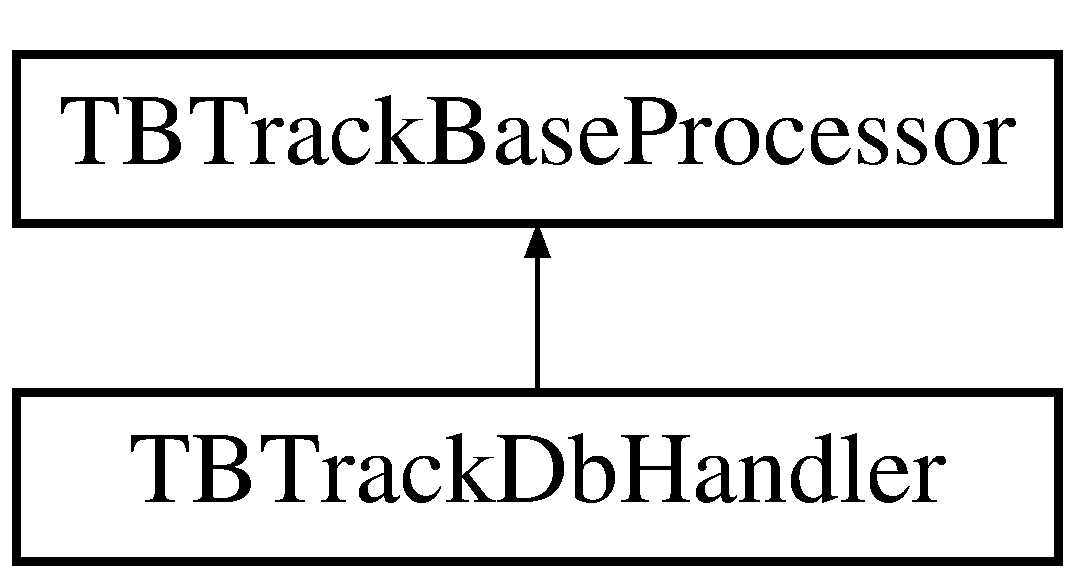
\includegraphics[height=2cm]{classTBTrackDbHandler}
\end{center}
\end{figure}
\subsection*{Public Member Functions}
\begin{DoxyCompactItemize}
\item 
virtual Processor $\ast$ {\bfseries newProcessor} ()\label{classTBTrackDbHandler_abe806895dc04980136469ac90bcc9982}

\item 
virtual void {\bfseries Init} ()\label{classTBTrackDbHandler_a57e8094c85725134aa69b7fbf7b7b8eb}

\item 
virtual void {\bfseries ProcessRunHeader} (LCRunHeader $\ast$run)\label{classTBTrackDbHandler_afc16f115885dc980dd75aaa41efceb81}

\item 
virtual void {\bfseries ProcessEvent} (LCEvent $\ast$evt)\label{classTBTrackDbHandler_aab729168e31d8f81a28800164444cadc}

\item 
virtual void {\bfseries End} ()\label{classTBTrackDbHandler_a2db2ea2c3d53cd585a21f5130def6732}

\end{DoxyCompactItemize}


\subsection{Detailed Description}


Definition at line 12 of file TBTrackDbHandler.hh.

The documentation for this class was generated from the following files:\begin{DoxyCompactItemize}
\item 
TBTrackDbHandler.hh\item 
TBTrackDbHandler.cc\end{DoxyCompactItemize}

\section{TBTrackMapper Class Reference}
\label{classTBTrackMapper}\index{TBTrackMapper@{TBTrackMapper}}
Inheritance diagram for TBTrackMapper::\begin{figure}[H]
\begin{center}
\leavevmode
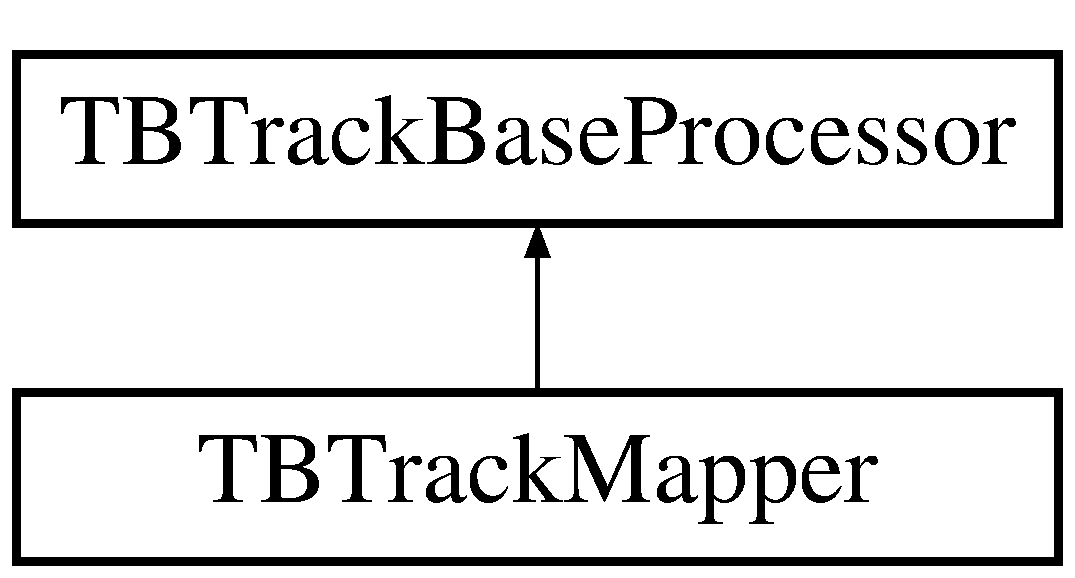
\includegraphics[height=2cm]{classTBTrackMapper}
\end{center}
\end{figure}
\subsection*{Public Member Functions}
\begin{DoxyCompactItemize}
\item 
{\bf TBTrackMapper} ()\label{classTBTrackMapper_ab5ebcbd9676bf78ae9633c8de9890842}

\begin{DoxyCompactList}\small\item\em Default constructor. \item\end{DoxyCompactList}\item 
void {\bf Init} ()\label{classTBTrackMapper_afc74449035c4cdfa91e5cdb7ac510c7f}

\begin{DoxyCompactList}\small\item\em Initialize the job -\/ called at the end of the \doxyref{TBTrackBaseProcessor::init}{p.}{classTBTrackBaseProcessor_a179b559dd67f1777b0622775918ae5f5} method. \item\end{DoxyCompactList}\item 
void {\bf ProcessRunHeader} (LCRunHeader $\ast$run)\label{classTBTrackMapper_a3992257a50060452146847f947787ee3}

\begin{DoxyCompactList}\small\item\em Process a RunHeader -\/ called at the end of the \doxyref{TBTrackBaseProcessor::processRunHeader}{p.}{classTBTrackBaseProcessor_a0fc18422f19b4c46ec4356df49b216c9} method. \item\end{DoxyCompactList}\item 
void {\bf ProcessEvent} (LCEvent $\ast$evtP)\label{classTBTrackMapper_a062f7399a3685671bc37e85636dba413}

\begin{DoxyCompactList}\small\item\em Process an Event -\/ called at the end of the \doxyref{TBTrackBaseProcessor::processEvent}{p.}{classTBTrackBaseProcessor_aba4e5b25679936687667e81f3a73df72} method. \item\end{DoxyCompactList}\item 
void {\bf End} ()\label{classTBTrackMapper_acd9bc1df4545f12184a40c8f0de8fb44}

\begin{DoxyCompactList}\small\item\em End of job -\/ called at the end of the \doxyref{TBTrackBaseProcessor::end}{p.}{classTBTrackBaseProcessor_aafbf0e1c1af756ea03748e482883d763} method. \item\end{DoxyCompactList}\item 
Processor $\ast$ {\bfseries newProcessor} ()\label{classTBTrackMapper_a109169447ef39058c87f0c90cf083960}

\end{DoxyCompactItemize}
\subsection*{Private Types}
\begin{DoxyCompactItemize}
\item 
typedef std::map$<$ int, CALICE::TdcConnection $>$ {\bfseries mMap\_\-t}\label{classTBTrackMapper_ab98758e67c8c14c2f6eeb7cf9ca32148}

\item 
typedef lccd::ConditionsMap$<$ int, CALICE::TdcConnection $>$ {\bfseries cMap\_\-t}\label{classTBTrackMapper_a2a5e17aaeb3c5c804d61c3fad958c037}

\item 
typedef std::vector$<$ int $>$ {\bfseries value\_\-t}\label{classTBTrackMapper_a9e308f613981ec6f042eb2fc2abc86be}

\item 
typedef std::map$<$ int, value\_\-t $>$ {\bfseries vMap\_\-t}\label{classTBTrackMapper_afac11c19152680213f1aeb5635063f09}

\end{DoxyCompactItemize}
\subsection*{Private Member Functions}
\begin{DoxyCompactItemize}
\item 
void {\bfseries reset} ()\label{classTBTrackMapper_aeae4c8ff7fc12d0fa84d72f4c4f206fd}

\item 
void {\bfseries findEdges} (LCEvent $\ast$evtP, EVENT::LCCollection $\ast$)\label{classTBTrackMapper_ad19dc2f9ee3eb973e27917e0c5f2400b}

\item 
void {\bfseries findHits} ()\label{classTBTrackMapper_a539cb5f99393b6100941569457931acb}

\item 
EVENT::LCCollection $\ast$ {\bfseries outputCollection} (const vMap\_\-t \&)\label{classTBTrackMapper_a22832aad26dcdab437dcb8227e209805}

\end{DoxyCompactItemize}
\subsection*{Private Attributes}
\begin{DoxyCompactItemize}
\item 
std::string {\bfseries \_\-TDCHitColName}\label{classTBTrackMapper_a84f41d60fa4d903d6b9b72f0fd7a8434}

\item 
std::string {\bfseries \_\-mappingColName}\label{classTBTrackMapper_acccd87de333eb8fc4ccd259536c51e3f}

\item 
int {\bfseries \_\-TDC\_\-Upper\_\-Limit}\label{classTBTrackMapper_a1a12022244828150ad3d298587f2eb66}

\item 
int {\bfseries \_\-TDC\_\-Lower\_\-Limit}\label{classTBTrackMapper_a0ab5b929b377e27f458b2fbd02af098d}

\item 
bool {\bfseries \_\-TDC\_\-CAEN1290}\label{classTBTrackMapper_afbbcdc5d206eed3c3e9b98182127c9cb}

\item 
cMap\_\-t $\ast$ {\bfseries \_\-mapping}\label{classTBTrackMapper_a50fddfd0670abbe51afd7c4b172e2ac7}

\item 
vMap\_\-t {\bfseries \_\-edges}\label{classTBTrackMapper_a5928cb0b84cd019aba35998fd8145fa5}

\item 
vMap\_\-t {\bfseries \_\-hits}\label{classTBTrackMapper_a900dee2c64d639ad2d153c31fdad7929}

\item 
bool {\bfseries \_\-twoLines}\label{classTBTrackMapper_a63f57f4d4e27254b508a628bd3a89d29}

\item 
bool {\bfseries \_\-firstEvent}\label{classTBTrackMapper_a6960324522d074a94d1e78b21e5a4724}

\end{DoxyCompactItemize}


\subsection{Detailed Description}


Definition at line 14 of file TBTrackMapper.hh.

The documentation for this class was generated from the following files:\begin{DoxyCompactItemize}
\item 
TBTrackMapper.hh\item 
TBTrackMapper.cc\end{DoxyCompactItemize}

\section{TBTrackMokkaCheck Class Reference}
\label{classTBTrackMokkaCheck}\index{TBTrackMokkaCheck@{TBTrackMokkaCheck}}
Inheritance diagram for TBTrackMokkaCheck::\begin{figure}[H]
\begin{center}
\leavevmode
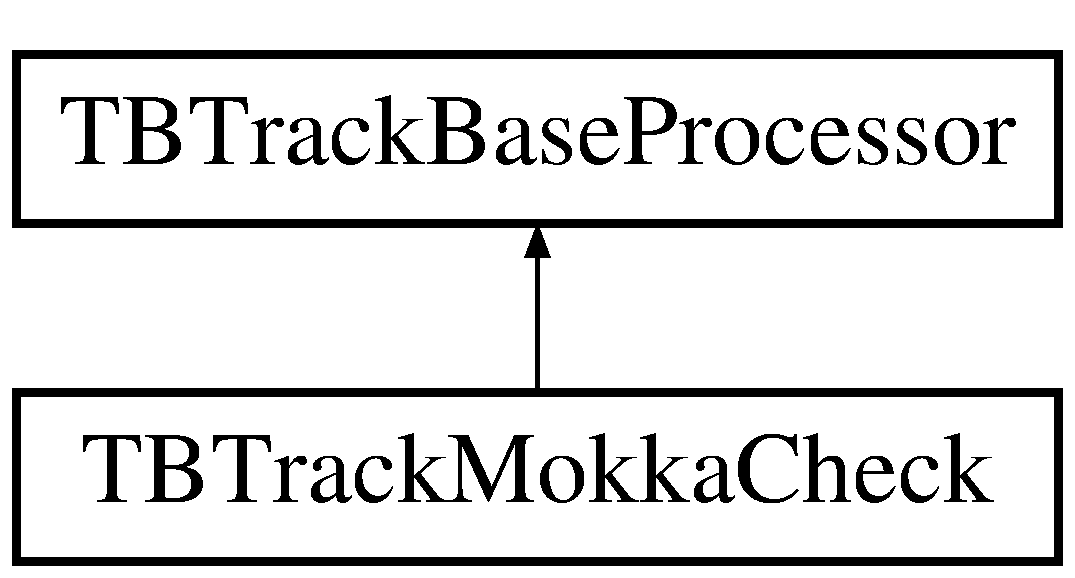
\includegraphics[height=2cm]{classTBTrackMokkaCheck}
\end{center}
\end{figure}
\subsection*{Public Member Functions}
\begin{DoxyCompactItemize}
\item 
virtual marlin::Processor $\ast$ {\bfseries newProcessor} ()\label{classTBTrackMokkaCheck_a53be3d2fd82b398eef9af471d4fd1f24}

\item 
virtual void {\bf Init} ()\label{classTBTrackMokkaCheck_abb8d8804a7ad6d130daa617910c82025}

\begin{DoxyCompactList}\small\item\em Called at the begin of the job. \item\end{DoxyCompactList}\item 
virtual void {\bf ProcessRunHeader} (LCRunHeader $\ast$run)\label{classTBTrackMokkaCheck_ae3ce319a159844c0b5eb130b52f823df}

\begin{DoxyCompactList}\small\item\em Called for every run. \item\end{DoxyCompactList}\item 
virtual void {\bf ProcessEvent} (LCEvent $\ast$evt)\label{classTBTrackMokkaCheck_ab7f2e45d6b34e294acf7be9084915031}

\begin{DoxyCompactList}\small\item\em Called for every event -\/ the working horse. \item\end{DoxyCompactList}\item 
virtual void {\bf End} ()\label{classTBTrackMokkaCheck_a10638273c995610da878db1eec2d27f6}

\begin{DoxyCompactList}\small\item\em Called after data processing for clean up. \item\end{DoxyCompactList}\item 
virtual void {\bfseries initHists} ()\label{classTBTrackMokkaCheck_a8c6b1f94938fcfb5a5aa4639135dac83}

\end{DoxyCompactItemize}
\subsection*{Private Attributes}
\begin{DoxyCompactItemize}
\item 
TH1F $\ast$ {\bfseries hNCol}\label{classTBTrackMokkaCheck_a0c9c9c99f9b716dd1992bb4ef4dc9752}

\item 
TH1F $\ast$ {\bfseries hNEnt}\label{classTBTrackMokkaCheck_a82a95f726f0c9a6143a9841194f99352}

\item 
TH1F $\ast$ {\bfseries hNumb} [2][4]\label{classTBTrackMokkaCheck_a4b8496fa6e482d1b766d2a1bc4ea5601}

\item 
TH1F $\ast$ {\bfseries hCell} [2][4]\label{classTBTrackMokkaCheck_a8039a6724748c468801aed23e01069da}

\item 
TH1F $\ast$ {\bfseries hPosn} [2][4]\label{classTBTrackMokkaCheck_a18d21b8473903ebd1064262b5845411d}

\item 
TH1F $\ast$ {\bfseries hPosz} [2][4]\label{classTBTrackMokkaCheck_a1bf5a8ba5867ded6b37099192f65f233}

\item 
TH1F $\ast$ {\bfseries hEner} [2][4]\label{classTBTrackMokkaCheck_a206f00deb9d1f038f90c298885089a00}

\item 
TH1F $\ast$ {\bfseries hTime} [2][4]\label{classTBTrackMokkaCheck_a041d981e1fcd92559e117112986ef83d}

\item 
TH1F $\ast$ {\bfseries hTana} [2][4]\label{classTBTrackMokkaCheck_aca36bbd029605cb2ae4a0ca7c575ca65}

\end{DoxyCompactItemize}


\subsection{Detailed Description}


Definition at line 17 of file TBTrackMokkaCheck.hh.

The documentation for this class was generated from the following files:\begin{DoxyCompactItemize}
\item 
TBTrackMokkaCheck.hh\item 
TBTrackMokkaCheck.cc\end{DoxyCompactItemize}

\section{TBTrackProducer Class Reference}
\label{classTBTrackProducer}\index{TBTrackProducer@{TBTrackProducer}}
Inheritance diagram for TBTrackProducer::\begin{figure}[H]
\begin{center}
\leavevmode
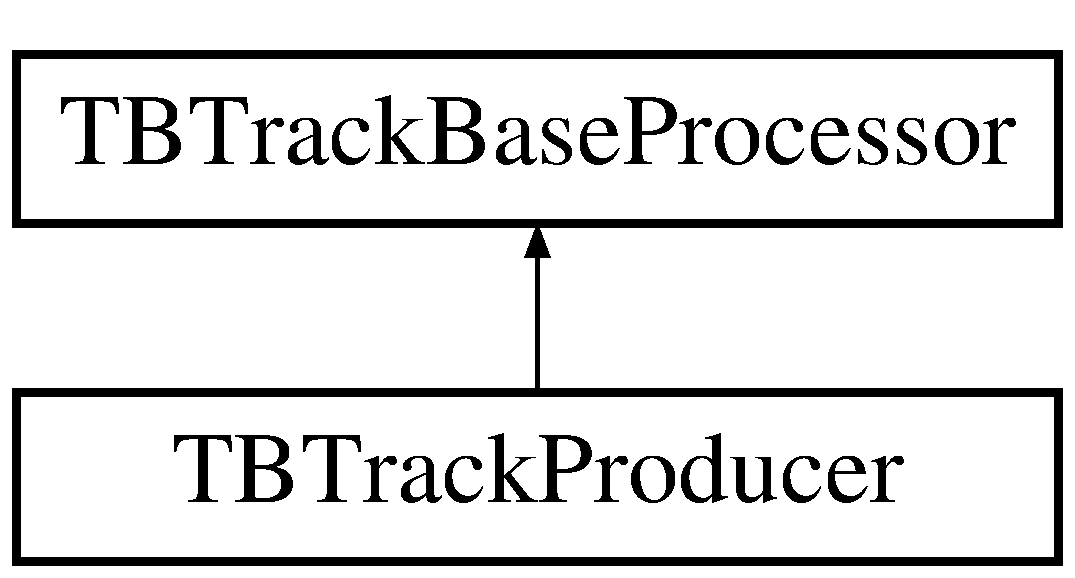
\includegraphics[height=2cm]{classTBTrackProducer}
\end{center}
\end{figure}
\subsection*{Public Member Functions}
\begin{DoxyCompactItemize}
\item 
virtual marlin::Processor $\ast$ {\bfseries newProcessor} ()\label{classTBTrackProducer_a5159c5af2b5661e0e0a7bfc7591217a9}

\item 
virtual void {\bf Init} ()\label{classTBTrackProducer_a261213eb92718b68b315253b056be414}

\begin{DoxyCompactList}\small\item\em Called at the begin of the job before anything is read. \item\end{DoxyCompactList}\item 
virtual void {\bf ProcessRunHeader} (LCRunHeader $\ast$run)\label{classTBTrackProducer_ac8c608a27e729c78ced0ec8b1969ca24}

\begin{DoxyCompactList}\small\item\em Called for every run. \item\end{DoxyCompactList}\item 
virtual void {\bf ProcessEvent} (LCEvent $\ast$evt)\label{classTBTrackProducer_a4aabdb65ff27029731aa3ce567ed528c}

\begin{DoxyCompactList}\small\item\em Called for every event -\/ the working horse. \item\end{DoxyCompactList}\item 
virtual void {\bf End} ()\label{classTBTrackProducer_a0294d07e812929d30d0797a15de7958b}

\begin{DoxyCompactList}\small\item\em Called after data processing for clean up. \item\end{DoxyCompactList}\end{DoxyCompactItemize}
\subsection*{Private Attributes}
\begin{DoxyCompactItemize}
\item 
{\bf TBTrack::TrackFinder} {\bfseries \_\-finder}\label{classTBTrackProducer_af6ef70618261f9e609a35018aba95110}

\item 
std::string {\bf \_\-TDCHitColName}\label{classTBTrackProducer_aaa9b990c825fb14a9b0a16254dc65cea}

\begin{DoxyCompactList}\small\item\em name of the Track output collection \item\end{DoxyCompactList}\end{DoxyCompactItemize}


\subsection{Detailed Description}


Definition at line 13 of file TBTrackProducer.hh.

The documentation for this class was generated from the following files:\begin{DoxyCompactItemize}
\item 
TBTrackProducer.hh\item 
TBTrackProducer.cc\end{DoxyCompactItemize}

\section{TBTrackProducerCheck Class Reference}
\label{classTBTrackProducerCheck}\index{TBTrackProducerCheck@{TBTrackProducerCheck}}
Inheritance diagram for TBTrackProducerCheck::\begin{figure}[H]
\begin{center}
\leavevmode
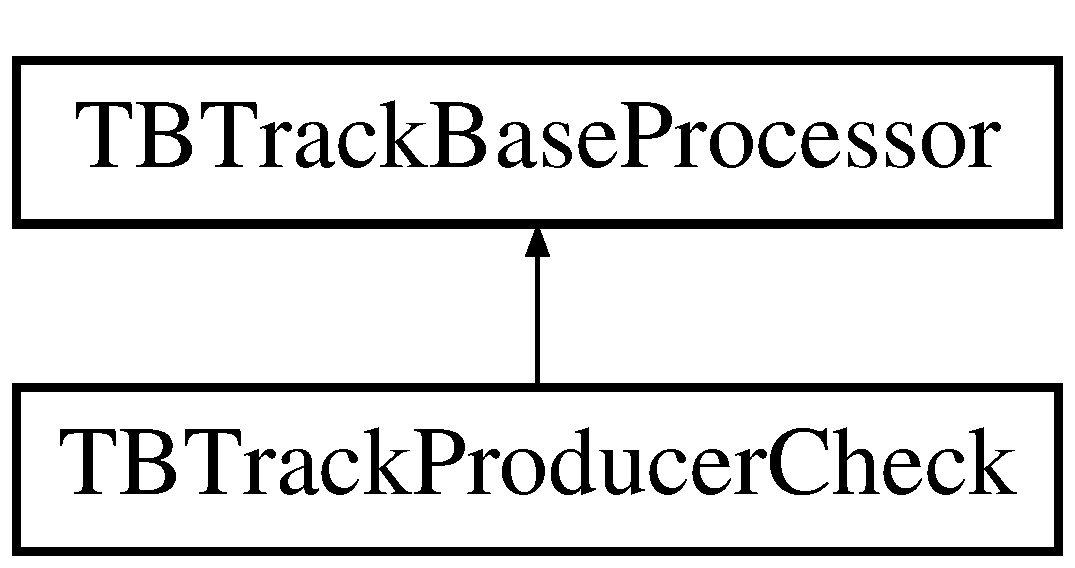
\includegraphics[height=2cm]{classTBTrackProducerCheck}
\end{center}
\end{figure}
\subsection*{Public Member Functions}
\begin{DoxyCompactItemize}
\item 
virtual Processor $\ast$ {\bfseries newProcessor} ()\label{classTBTrackProducerCheck_a52c88c93fa514c84d0fa64d7b9a91bb4}

\item 
virtual void {\bf Init} ()
\begin{DoxyCompactList}\small\item\em Called at the begin of the job before anything is read. \item\end{DoxyCompactList}\item 
virtual void {\bfseries initHists} (unsigned p, bool t)\label{classTBTrackProducerCheck_ab8db52f3eac5938feed32c631ec33e85}

\item 
virtual void {\bf ProcessRunHeader} (LCRunHeader $\ast$run)\label{classTBTrackProducerCheck_ad4e1b5a9d27c078a6d5b20c200b51823}

\begin{DoxyCompactList}\small\item\em Called for every run. \item\end{DoxyCompactList}\item 
virtual void {\bf ProcessEvent} (LCEvent $\ast$evt)\label{classTBTrackProducerCheck_ac83ba8232136941271cfef652836094d}

\begin{DoxyCompactList}\small\item\em Called for every event -\/ the working horse. \item\end{DoxyCompactList}\item 
virtual void {\bf End} ()\label{classTBTrackProducerCheck_a04fd5ebf531bdba12e07c9da6aeb5f46}

\begin{DoxyCompactList}\small\item\em Called after data processing for clean up. \item\end{DoxyCompactList}\end{DoxyCompactItemize}
\subsection*{Private Attributes}
\begin{DoxyCompactItemize}
\item 
TH1F $\ast$ {\bf hNumb} [2][17]\label{classTBTrackProducerCheck_a312c63e82786bcf37cb73181499d901e}

\begin{DoxyCompactList}\small\item\em Method to write the histograms in a ROOT file. \item\end{DoxyCompactList}\item 
TH1F $\ast$ {\bfseries hPatt} [2][17]\label{classTBTrackProducerCheck_afb76754f76b38f3dc7462558a8932be3}

\item 
TH1F $\ast$ {\bfseries hPar0} [2][17]\label{classTBTrackProducerCheck_a43606e256daf8d35f04084ed6be3ed90}

\item 
TH1F $\ast$ {\bfseries hPar1} [2][17]\label{classTBTrackProducerCheck_a30564020aa68a8b3c6106c3b4a450370}

\item 
TH1F $\ast$ {\bfseries hErr0} [2][17]\label{classTBTrackProducerCheck_a05abcd6e8fa279cd0f2323776522ffc4}

\item 
TH1F $\ast$ {\bfseries hErr1} [2][17]\label{classTBTrackProducerCheck_aa3904bfd80ad62890136a8c703bc80ff}

\item 
TH1F $\ast$ {\bfseries hCorr} [2][17]\label{classTBTrackProducerCheck_a8d2a10d2c363416d792a52dac273e940}

\item 
TH1F $\ast$ {\bfseries hProb} [2][17]\label{classTBTrackProducerCheck_a7a20c547f7cea4fc2f96430c61596509}

\item 
TH1F $\ast$ {\bfseries hHits} [2][17][4]\label{classTBTrackProducerCheck_afad31cbb959ca8bf00c9dcd4f1f5608c}

\item 
TH2F $\ast$ {\bfseries hNmb2} [2][17]\label{classTBTrackProducerCheck_a537737addf64198ef899b544e5bcc56a}

\item 
TH2F $\ast$ {\bfseries hPrb2} [2][17]\label{classTBTrackProducerCheck_ad89eaff5c26155f0be4a2a90b1be18c2}

\item 
TH1F $\ast$ {\bfseries hMPr0} [2][17]\label{classTBTrackProducerCheck_a9e9c5ec4dc1ded9f7f5db19201c4cd80}

\item 
TH1F $\ast$ {\bfseries hMPr1} [2][17]\label{classTBTrackProducerCheck_a20fa167b71982b48ae9d40b4ee77257c}

\item 
TH1F $\ast$ {\bfseries hMDf0} [2][17]\label{classTBTrackProducerCheck_ac124b49e9093d72ed02cbaa83fe025ec}

\item 
TH1F $\ast$ {\bfseries hMDf1} [2][17]\label{classTBTrackProducerCheck_ab7a5a04286cfad781a1764ae54c4d2b1}

\end{DoxyCompactItemize}


\subsection{Detailed Description}


Definition at line 17 of file TBTrackProducerCheck.hh.

\subsection{Member Function Documentation}
\index{TBTrackProducerCheck@{TBTrackProducerCheck}!Init@{Init}}
\index{Init@{Init}!TBTrackProducerCheck@{TBTrackProducerCheck}}
\subsubsection[{Init}]{\setlength{\rightskip}{0pt plus 5cm}void TBTrackProducerCheck::Init ()\hspace{0.3cm}{\ttfamily  [virtual]}}\label{classTBTrackProducerCheck_a12c14a16f9145b8f04ca63f731e540f4}


Called at the begin of the job before anything is read. Use to initialize the processor, e.g. book histograms. 

Implements {\bf TBTrackBaseProcessor} \doxyref{}{p.}{classTBTrackBaseProcessor}.

Definition at line 97 of file TBTrackProducerCheck.cc.

The documentation for this class was generated from the following files:\begin{DoxyCompactItemize}
\item 
TBTrackProducerCheck.hh\item 
TBTrackProducerCheck.cc\end{DoxyCompactItemize}

\section{TBTrackRawCheck Class Reference}
\label{classTBTrackRawCheck}\index{TBTrackRawCheck@{TBTrackRawCheck}}
Inheritance diagram for TBTrackRawCheck::\begin{figure}[H]
\begin{center}
\leavevmode
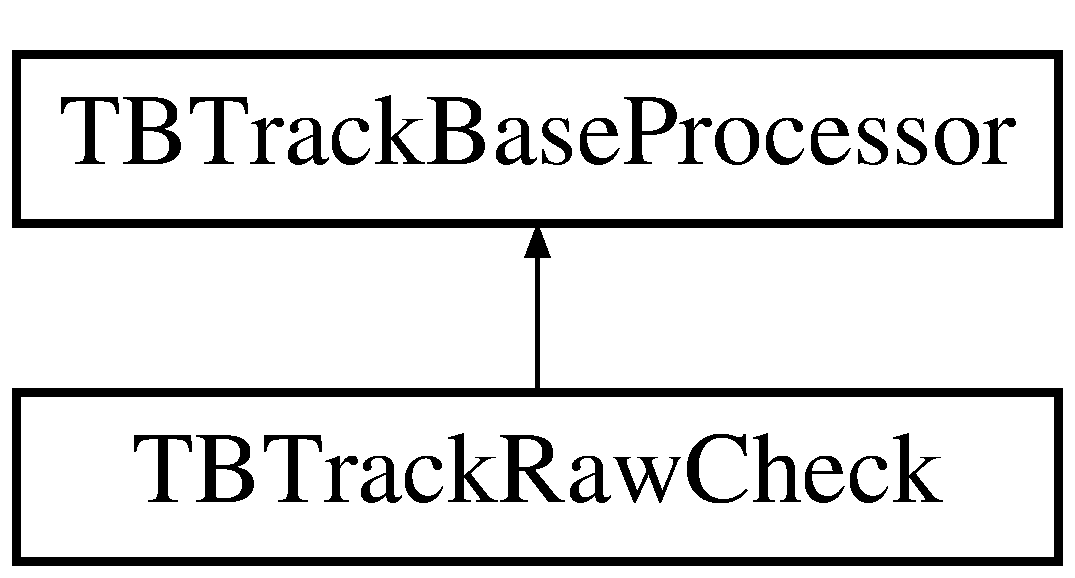
\includegraphics[height=2cm]{classTBTrackRawCheck}
\end{center}
\end{figure}
\subsection*{Public Member Functions}
\begin{DoxyCompactItemize}
\item 
virtual Processor $\ast$ {\bfseries newProcessor} ()\label{classTBTrackRawCheck_af6d15c223523fea01a128d1ac3f01ae8}

\item 
virtual void {\bf Init} ()
\begin{DoxyCompactList}\small\item\em Called at the begin of the job before anything is read. \item\end{DoxyCompactList}\item 
virtual void {\bf ProcessRunHeader} (LCRunHeader $\ast$run)\label{classTBTrackRawCheck_a4f53d3aaff6320d3bab282cacde1e8bb}

\begin{DoxyCompactList}\small\item\em Called for every run. \item\end{DoxyCompactList}\item 
virtual void {\bf ProcessEvent} (LCEvent $\ast$evt)\label{classTBTrackRawCheck_ad8ced9850a3da2532df3a65375678d0f}

\begin{DoxyCompactList}\small\item\em Called for every event -\/ the working horse. \item\end{DoxyCompactList}\item 
virtual void {\bf End} ()\label{classTBTrackRawCheck_a0b2e05deaa1a9e475894473bfe34a4c5}

\begin{DoxyCompactList}\small\item\em Called after data processing for clean up. \item\end{DoxyCompactList}\item 
virtual void {\bfseries initHists} (bool real)\label{classTBTrackRawCheck_a8fe77bfd27cd1d49f13b87127723131e}

\end{DoxyCompactItemize}
\subsection*{Private Attributes}
\begin{DoxyCompactItemize}
\item 
bool {\bf \_\-cern}\label{classTBTrackRawCheck_a5072e5d27ead3cb9d0265658081d4588}

\begin{DoxyCompactList}\small\item\em Method to write the histograms in a ROOT file. \item\end{DoxyCompactList}\item 
TH1F $\ast$ {\bfseries hDist} [16]\label{classTBTrackRawCheck_ae377100f20e9ff77dff6efa691ebea3b}

\item 
TH2F $\ast$ {\bfseries hDi2d} [16]\label{classTBTrackRawCheck_af8a6fffae88fb979618e72d43b066894}

\item 
TH1F $\ast$ {\bfseries hDi2p} [16]\label{classTBTrackRawCheck_a8be318c350a3894f49227751b6bae9b7}

\item 
TH1F $\ast$ {\bfseries hDi2m} [16]\label{classTBTrackRawCheck_ad125fd66e3abb8bb028309fea49190d7}

\end{DoxyCompactItemize}


\subsection{Detailed Description}


Definition at line 22 of file TBTrackRawCheck.hh.

\subsection{Member Function Documentation}
\index{TBTrackRawCheck@{TBTrackRawCheck}!Init@{Init}}
\index{Init@{Init}!TBTrackRawCheck@{TBTrackRawCheck}}
\subsubsection[{Init}]{\setlength{\rightskip}{0pt plus 5cm}void TBTrackRawCheck::Init ()\hspace{0.3cm}{\ttfamily  [virtual]}}\label{classTBTrackRawCheck_ad50f762bb554e9b827d9a921e2f1de9c}


Called at the begin of the job before anything is read. Use to initialize the processor, e.g. book histograms. 

Implements {\bf TBTrackBaseProcessor} \doxyref{}{p.}{classTBTrackBaseProcessor}.

Definition at line 81 of file TBTrackRawCheck.cc.

The documentation for this class was generated from the following files:\begin{DoxyCompactItemize}
\item 
TBTrackRawCheck.hh\item 
TBTrackRawCheck.cc\end{DoxyCompactItemize}

\section{marlin::TBTrackRemover Class Reference}
\label{classmarlin_1_1TBTrackRemover}\index{marlin::TBTrackRemover@{marlin::TBTrackRemover}}


Preprocessor which is supposed to run at the !very! beginning of the processor chain.  


{\ttfamily \#include $<$TBTrackRemover.hh$>$}\subsection*{Data Structures}
\begin{DoxyCompactItemize}
\item 
class {\bf LCEventModifier}
\begin{DoxyCompactList}\small\item\em Helper class to for the modification of the Event Header. \item\end{DoxyCompactList}\end{DoxyCompactItemize}
\subsection*{Public Member Functions}
\begin{DoxyCompactItemize}
\item 
virtual Processor $\ast$ {\bfseries newProcessor} ()\label{classmarlin_1_1TBTrackRemover_aabd6f4686ad80cd4dc5c00ad485532ab}

\item 
virtual void {\bf init} ()
\begin{DoxyCompactList}\small\item\em Called at the begin of the job before anything is read. \item\end{DoxyCompactList}\item 
virtual void {\bf processRunHeader} (LCRunHeader $\ast$run)\label{classmarlin_1_1TBTrackRemover_a7a4a783bba99c63bf4dfd424a39b461a}

\begin{DoxyCompactList}\small\item\em Called for every run. \item\end{DoxyCompactList}\item 
virtual void {\bf processEvent} (LCEvent $\ast$evt)\label{classmarlin_1_1TBTrackRemover_a6a9ccb473b3383d1ccb978e3ba8a7760}

\begin{DoxyCompactList}\small\item\em Called for every event -\/ the working horse. \item\end{DoxyCompactList}\item 
virtual void {\bfseries check} (LCEvent $\ast$evt)\label{classmarlin_1_1TBTrackRemover_a24007dc2befc665be3688fc38683e002}

\item 
virtual void {\bf end} ()\label{classmarlin_1_1TBTrackRemover_af53b200afa75c5e10cc2fe2ccb19672b}

\begin{DoxyCompactList}\small\item\em Called after data processing for clean up. \item\end{DoxyCompactList}\end{DoxyCompactItemize}


\subsection{Detailed Description}
Preprocessor which is supposed to run at the !very! beginning of the processor chain. Adding information to the Run and EventHeader.for data and MC. In partcular the beam energy is extracted from the database for a given run and the MC events get assigned a timestamp. \begin{DoxyAuthor}{Author}
: A.M. Magnan Imperial College, modifs R.Poeschl LAL
\end{DoxyAuthor}
\begin{DoxyDate}{Date}
Apr 2007 
\end{DoxyDate}


Definition at line 38 of file TBTrackRemover.hh.

\subsection{Member Function Documentation}
\index{marlin::TBTrackRemover@{marlin::TBTrackRemover}!init@{init}}
\index{init@{init}!marlin::TBTrackRemover@{marlin::TBTrackRemover}}
\subsubsection[{init}]{\setlength{\rightskip}{0pt plus 5cm}void marlin::TBTrackRemover::init ()\hspace{0.3cm}{\ttfamily  [virtual]}}\label{classmarlin_1_1TBTrackRemover_a48e9f5ce74d8a9798a533dd276c988c0}


Called at the begin of the job before anything is read. Use to initialize the processor, e.g. book histograms. 

Definition at line 82 of file TBTrackRemover.cc.

The documentation for this class was generated from the following files:\begin{DoxyCompactItemize}
\item 
TBTrackRemover.hh\item 
TBTrackRemover.cc\end{DoxyCompactItemize}

\section{TBTrackScatter Class Reference}
\label{classTBTrackScatter}\index{TBTrackScatter@{TBTrackScatter}}
Inheritance diagram for TBTrackScatter::\begin{figure}[H]
\begin{center}
\leavevmode
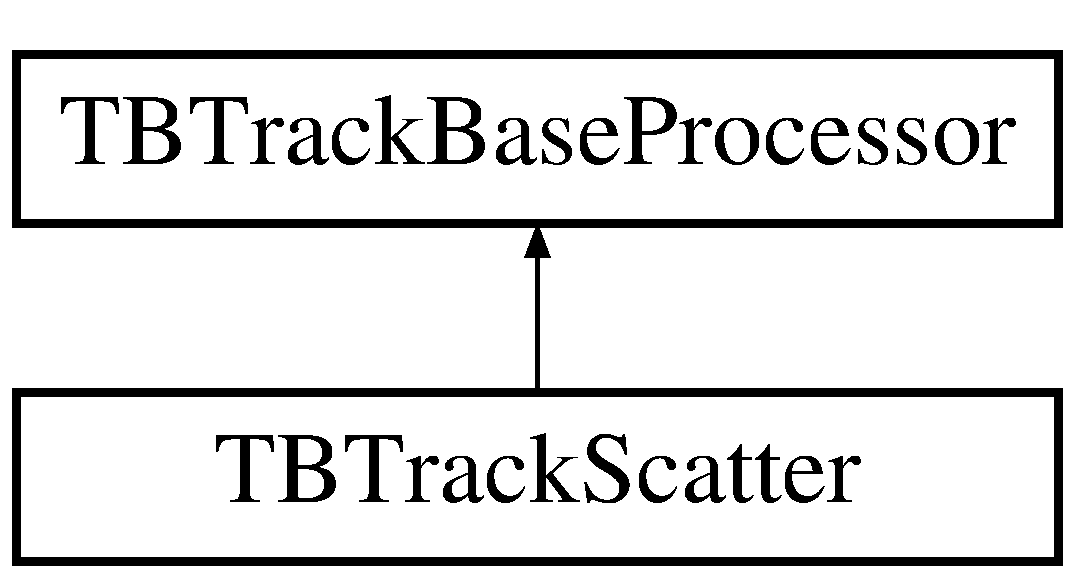
\includegraphics[height=2cm]{classTBTrackScatter}
\end{center}
\end{figure}
\subsection*{Data Structures}
\begin{DoxyCompactItemize}
\item 
class {\bf TBEvent}
\end{DoxyCompactItemize}
\subsection*{Public Member Functions}
\begin{DoxyCompactItemize}
\item 
virtual Processor $\ast$ {\bfseries newProcessor} ()\label{classTBTrackScatter_add1e78763f106644f161ba177f5f21e3}

\item 
virtual void {\bfseries Init} ()\label{classTBTrackScatter_a82431b4518ed55dbdf953ac15cdfc710}

\item 
virtual void {\bfseries ProcessRunHeader} (LCRunHeader $\ast$run)\label{classTBTrackScatter_ae27794c29359577e8278753bb7c74ead}

\item 
virtual void {\bfseries ProcessEvent} (LCEvent $\ast$evt)\label{classTBTrackScatter_a328a0b121402a3779882e39ecc575934}

\item 
virtual void {\bfseries End} ()\label{classTBTrackScatter_a1c5d977fb520115d85706dd7f3794edd}

\item 
TMatrixDSym {\bfseries findError} (const std::vector$<$ TVectorD $>$ \&v, double cutProb=0.1, bool mean=true)\label{classTBTrackScatter_aa6ff59b2691627b05c8726740215c81a}

\item 
void {\bfseries findError2} ()\label{classTBTrackScatter_a4350eab83583bce7b782f95bf9ffca20}

\item 
virtual void {\bfseries initHists} ()\label{classTBTrackScatter_ac27b4d5c266645c0b7869ec8301bb6af}

\end{DoxyCompactItemize}
\subsection*{Private Types}
\begin{DoxyCompactItemize}
\item 
enum \{ {\bfseries NLAYER} = 4, 
{\bfseries NPM} = 14, 
{\bfseries NDM} = 6, 
{\bfseries NEXTRAP} = 3
 \}
\end{DoxyCompactItemize}
\subsection*{Private Member Functions}
\begin{DoxyCompactItemize}
\item 
void {\bfseries getHitInfo} (LCEvent $\ast$evt)\label{classTBTrackScatter_ab1ea6e233c8bb77220d359f12a9c9157}

\item 
void {\bfseries fillHistograms} ({\bf TBEvent} $\ast$tbEvent)\label{classTBTrackScatter_a640bc27626ee6e00e65c38065a2d358a}

\item 
void {\bfseries fillHistograms} ()\label{classTBTrackScatter_ab72d09b02640fe451b58f87989b6b6bc}

\item 
double {\bfseries getTruncatedRMS} (TH1F $\ast$h, float factor=20.)\label{classTBTrackScatter_aece42b823239fe34a46c3497718acb76}

\end{DoxyCompactItemize}
\subsection*{Private Attributes}
\begin{DoxyCompactItemize}
\item 
int {\bfseries \_\-oldRun}\label{classTBTrackScatter_a2372dac837987cb91190c765e88afe5e}

\item 
std::string {\bfseries \_\-simFakeTrackerHitCollection}\label{classTBTrackScatter_aa6588dd0c39bb7233713e0316aa79bf1}

\item 
std::vector$<$ TVectorD $>$ {\bfseries \_\-vDelta} [2]\label{classTBTrackScatter_a4cc08b20f1c47a776a17b0fbdf3b5cde}

\item 
std::vector$<$ {\bf TBEvent} $>$ {\bfseries \_\-vTBEvent}\label{classTBTrackScatter_a8b5488d90a4609d9ad0c76bd8b9eafc0}

\item 
TMatrixD {\bfseries \_\-rotation}\label{classTBTrackScatter_a6e0f3f493843e958a26f97abdf016719}

\item 
TH1F $\ast$ {\bfseries \_\-hZpos} [2][NLAYER+1]\label{classTBTrackScatter_a6346d26d8e806ce65a0c2c4988f0c4c1}

\item 
TH1F $\ast$ {\bfseries \_\-NEW\_\-hPos1d\_\-fake} [2]\label{classTBTrackScatter_a97015843273ab4a90ebeb8cdb69a4992}

\item 
TH1F $\ast$ {\bfseries \_\-NEW\_\-hPos1d\_\-mc} [2]\label{classTBTrackScatter_a19bbb91bc1540399f5eaee549556f316}

\item 
TH1F $\ast$ {\bfseries \_\-NEW\_\-hPos1d} [2][NEXTRAP][NLAYER]\label{classTBTrackScatter_a97b84e856a277819cd7f247ea60d44a6}

\item 
TH2F $\ast$ {\bfseries \_\-NEW\_\-hPos2d} [2][NEXTRAP][NLAYER $\ast$(NLAYER-\/1)/2]\label{classTBTrackScatter_a6603bd7007c65e8d0c1629f2aea1f28e}

\item 
TH2F $\ast$ {\bfseries \_\-NEW\_\-hPos2d\_\-rot} [2][NEXTRAP][NLAYER $\ast$(NLAYER-\/1)/2]\label{classTBTrackScatter_ad1e3af55a110dbf0643010d441081184}

\end{DoxyCompactItemize}
\subsection*{Static Private Attributes}
\begin{DoxyCompactItemize}
\item 
static const float {\bfseries \_\-rotationAngle} = TMath::Pi()/4.\label{classTBTrackScatter_afc07015eaaeb5336f43d061ab54dfc67}

\end{DoxyCompactItemize}


\subsection{Detailed Description}


Definition at line 27 of file TBTrackScatter.hh.

The documentation for this class was generated from the following files:\begin{DoxyCompactItemize}
\item 
TBTrackScatter.hh\item 
TBTrackScatter.cc\end{DoxyCompactItemize}

\section{TBTrackTdcHitsCheck Class Reference}
\label{classTBTrackTdcHitsCheck}\index{TBTrackTdcHitsCheck@{TBTrackTdcHitsCheck}}
Inheritance diagram for TBTrackTdcHitsCheck::\begin{figure}[H]
\begin{center}
\leavevmode
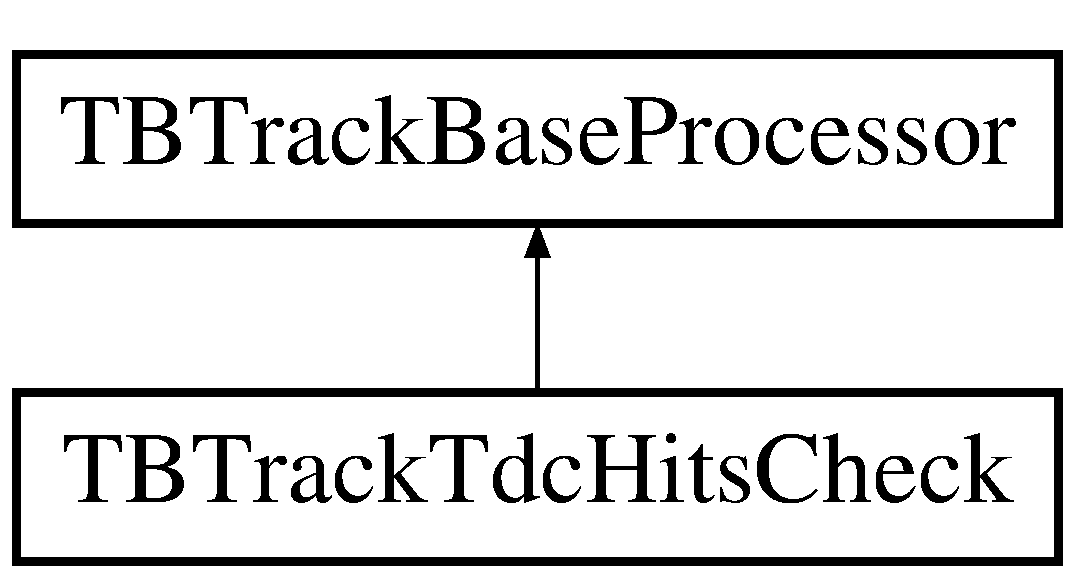
\includegraphics[height=2cm]{classTBTrackTdcHitsCheck}
\end{center}
\end{figure}
\subsection*{Public Member Functions}
\begin{DoxyCompactItemize}
\item 
virtual Processor $\ast$ {\bfseries newProcessor} ()\label{classTBTrackTdcHitsCheck_a4a3d12b82400668bbffe9b9a6993a97d}

\item 
virtual void {\bf Init} ()
\begin{DoxyCompactList}\small\item\em Called at the begin of the job before anything is read. \item\end{DoxyCompactList}\item 
virtual void {\bf ProcessRunHeader} (LCRunHeader $\ast$run)\label{classTBTrackTdcHitsCheck_af89a3701062f20bb205c4e8dd08e522c}

\begin{DoxyCompactList}\small\item\em Called for every run. \item\end{DoxyCompactList}\item 
virtual void {\bf ProcessEvent} (LCEvent $\ast$evt)\label{classTBTrackTdcHitsCheck_ac8199637e2c14163b67aa7be16e6b89f}

\begin{DoxyCompactList}\small\item\em Called for every event -\/ the working horse. \item\end{DoxyCompactList}\item 
virtual void {\bf End} ()\label{classTBTrackTdcHitsCheck_a8e979db0b7d4f3396cee4fe0c07cac32}

\begin{DoxyCompactList}\small\item\em Called after data processing for clean up. \item\end{DoxyCompactList}\item 
virtual void {\bfseries initHists} (bool real)\label{classTBTrackTdcHitsCheck_a0a37f04069e36ffb78182a6154c2944b}

\end{DoxyCompactItemize}
\subsection*{Private Attributes}
\begin{DoxyCompactItemize}
\item 
bool {\bf \_\-cern}\label{classTBTrackTdcHitsCheck_af989557649c4e709716ff4fb6ade30cb}

\begin{DoxyCompactList}\small\item\em Method to write the histograms in a ROOT file. \item\end{DoxyCompactList}\item 
TH1F $\ast$ {\bfseries hNCol}\label{classTBTrackTdcHitsCheck_a855f4e96cbe8858e152e10071d3e7b85}

\item 
TH1F $\ast$ {\bfseries hNEnt}\label{classTBTrackTdcHitsCheck_af977d14ce5313a7c93d4ccefb9cce998}

\item 
TH1F $\ast$ {\bfseries hNumb} [2][4]\label{classTBTrackTdcHitsCheck_aac7809c7921caea3c0e3bc624be02cf4}

\item 
TH1F $\ast$ {\bfseries hDist} [2][4]\label{classTBTrackTdcHitsCheck_af1e18036c82ca0374147c1119d1a0fcd}

\item 
TH1F $\ast$ {\bfseries hSepr} [2][4]\label{classTBTrackTdcHitsCheck_a10420c1a5f1a586a87b73ca0c013d9e8}

\item 
TH1F $\ast$ {\bfseries hLpmL} [2][6]\label{classTBTrackTdcHitsCheck_a6ab7fbde4baa6a6dbb11a821a8b04583}

\item 
TH2F $\ast$ {\bfseries hLvsL} [2][6]\label{classTBTrackTdcHitsCheck_ae4f5c1006e00659b2fa27d3bceabcd8f}

\item 
TH1F $\ast$ {\bfseries hDiff} [2][4]\label{classTBTrackTdcHitsCheck_a55fdb0e5a9c4358c3ac84ee8ab12971c}

\end{DoxyCompactItemize}


\subsection{Detailed Description}


Definition at line 22 of file TBTrackTdcHitsCheck.hh.

\subsection{Member Function Documentation}
\index{TBTrackTdcHitsCheck@{TBTrackTdcHitsCheck}!Init@{Init}}
\index{Init@{Init}!TBTrackTdcHitsCheck@{TBTrackTdcHitsCheck}}
\subsubsection[{Init}]{\setlength{\rightskip}{0pt plus 5cm}void TBTrackTdcHitsCheck::Init ()\hspace{0.3cm}{\ttfamily  [virtual]}}\label{classTBTrackTdcHitsCheck_a96a6fbe507db8ce20f3eaffdf661605a}


Called at the begin of the job before anything is read. Use to initialize the processor, e.g. book histograms. 

Implements {\bf TBTrackBaseProcessor} \doxyref{}{p.}{classTBTrackBaseProcessor}.

Definition at line 104 of file TBTrackTdcHitsCheck.cc.

The documentation for this class was generated from the following files:\begin{DoxyCompactItemize}
\item 
TBTrackTdcHitsCheck.hh\item 
TBTrackTdcHitsCheck.cc\end{DoxyCompactItemize}

\section{CALICE::TcmtMappingIIProcessor Class Reference}
\label{classCALICE_1_1TcmtMappingIIProcessor}\index{CALICE::TcmtMappingIIProcessor@{CALICE::TcmtMappingIIProcessor}}
Inheritance diagram for CALICE::TcmtMappingIIProcessor::\begin{figure}[H]
\begin{center}
\leavevmode
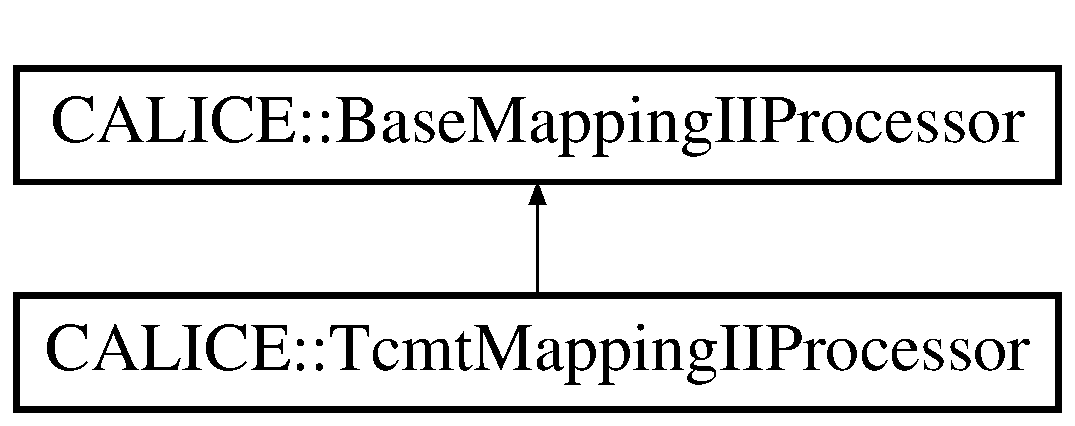
\includegraphics[height=2cm]{classCALICE_1_1TcmtMappingIIProcessor}
\end{center}
\end{figure}
\subsection*{Public Member Functions}
\begin{DoxyCompactItemize}
\item 
Processor $\ast$ {\bfseries newProcessor} ()\label{classCALICE_1_1TcmtMappingIIProcessor_ac417015d21a1632426336568a495a2fa}

\item 
void {\bfseries init} ()\label{classCALICE_1_1TcmtMappingIIProcessor_ace486ac86291c644b789d0aa08594c5c}

\item 
void {\bfseries processRunHeader} (LCRunHeader $\ast$run)\label{classCALICE_1_1TcmtMappingIIProcessor_a1a174e14b6a40294339c428a7a03b58a}

\item 
void {\bfseries processEvent} (LCEvent $\ast$evt)\label{classCALICE_1_1TcmtMappingIIProcessor_ad6fb82cdf2edfcf25c94b1ffcc6a2fc6}

\item 
void {\bfseries check} (LCEvent $\ast$evt)\label{classCALICE_1_1TcmtMappingIIProcessor_abc7540afa5e54c3f3908dfb9ef6691d7}

\item 
void {\bfseries end} ()\label{classCALICE_1_1TcmtMappingIIProcessor_aad749b67ac8b671bbb16bb52b49dd714}

\end{DoxyCompactItemize}
\subsection*{Private Attributes}
\begin{DoxyCompactItemize}
\item 
float {\bfseries \_\-energyThreshold}\label{classCALICE_1_1TcmtMappingIIProcessor_acf3598b6f599e7ec7c691b0995c86ca0}

\item 
int {\bfseries \_\-outputCollectionType}\label{classCALICE_1_1TcmtMappingIIProcessor_ad941439d1f231ec3ea9ca0cfdd25c142}

\end{DoxyCompactItemize}


\subsection{Detailed Description}


Definition at line 27 of file TcmtMappingIIProcessor.hh.

The documentation for this class was generated from the following files:\begin{DoxyCompactItemize}
\item 
TcmtMappingIIProcessor.hh\item 
TcmtMappingIIProcessor.cc\end{DoxyCompactItemize}

\section{CALICE::TcmtMappingIProcessor Class Reference}
\label{classCALICE_1_1TcmtMappingIProcessor}\index{CALICE::TcmtMappingIProcessor@{CALICE::TcmtMappingIProcessor}}
Inheritance diagram for CALICE::TcmtMappingIProcessor::\begin{figure}[H]
\begin{center}
\leavevmode
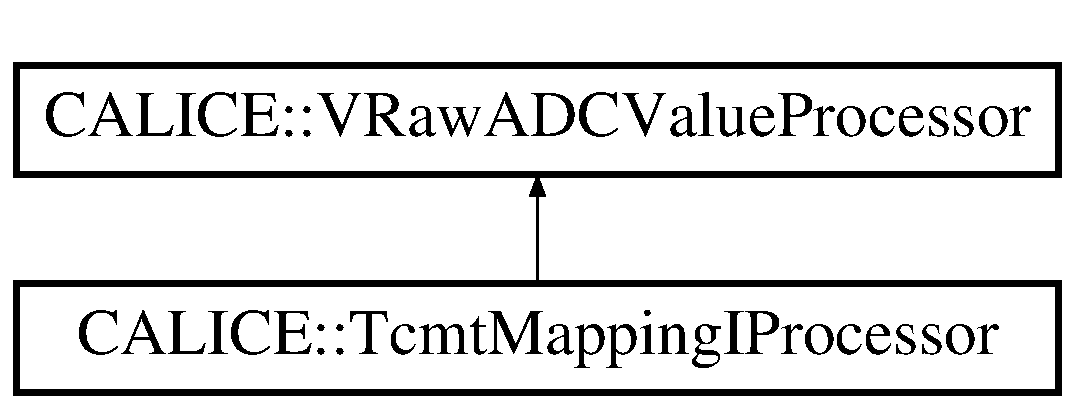
\includegraphics[height=2cm]{classCALICE_1_1TcmtMappingIProcessor}
\end{center}
\end{figure}
\subsection*{Public Member Functions}
\begin{DoxyCompactItemize}
\item 
virtual Processor $\ast$ {\bfseries newProcessor} ()\label{classCALICE_1_1TcmtMappingIProcessor_af68eccae5145606b935a16cb3c17a23f}

\item 
virtual void {\bfseries init} ()\label{classCALICE_1_1TcmtMappingIProcessor_ab2aacaee87955c83ede7a99d5bdcf6f9}

\item 
virtual void {\bfseries processRunHeader} (LCRunHeader $\ast$run)\label{classCALICE_1_1TcmtMappingIProcessor_a57645dbfce4fa856af7e3095baf98ebc}

\item 
virtual void {\bfseries processEvent} (LCEvent $\ast$evt)\label{classCALICE_1_1TcmtMappingIProcessor_afebd6aa1a8d9fbf9ee73994bc055992d}

\item 
virtual void {\bfseries check} (LCEvent $\ast$evt)\label{classCALICE_1_1TcmtMappingIProcessor_a7300f0af5983855142d7a7305b871203}

\item 
virtual void {\bfseries end} ()\label{classCALICE_1_1TcmtMappingIProcessor_aa25fac7f90f23cca521b526f1dfdaf95}

\end{DoxyCompactItemize}
\subsection*{Protected Attributes}
\begin{DoxyCompactItemize}
\item 
std::string {\bfseries \_\-outputColName}\label{classCALICE_1_1TcmtMappingIProcessor_a15cfbc83930d9bbdbfdc06e236a7ef85}

\item 
int {\bfseries \_\-viewConnectionTree}\label{classCALICE_1_1TcmtMappingIProcessor_ac01cd43e9ffa831e71f4b532f41e53ba}

\item 
int {\bfseries \_\-pickModule}\label{classCALICE_1_1TcmtMappingIProcessor_a410fc845042ea33a01a75014320c9022}

\end{DoxyCompactItemize}


\subsection{Detailed Description}


Definition at line 19 of file TcmtMappingIProcessor.hh.

The documentation for this class was generated from the following files:\begin{DoxyCompactItemize}
\item 
TcmtMappingIProcessor.hh\item 
TcmtMappingIProcessor.cc\end{DoxyCompactItemize}

\section{CALICE::TcmtOverlayProcessor Class Reference}
\label{classCALICE_1_1TcmtOverlayProcessor}\index{CALICE::TcmtOverlayProcessor@{CALICE::TcmtOverlayProcessor}}
Inheritance diagram for CALICE::TcmtOverlayProcessor::\begin{figure}[H]
\begin{center}
\leavevmode
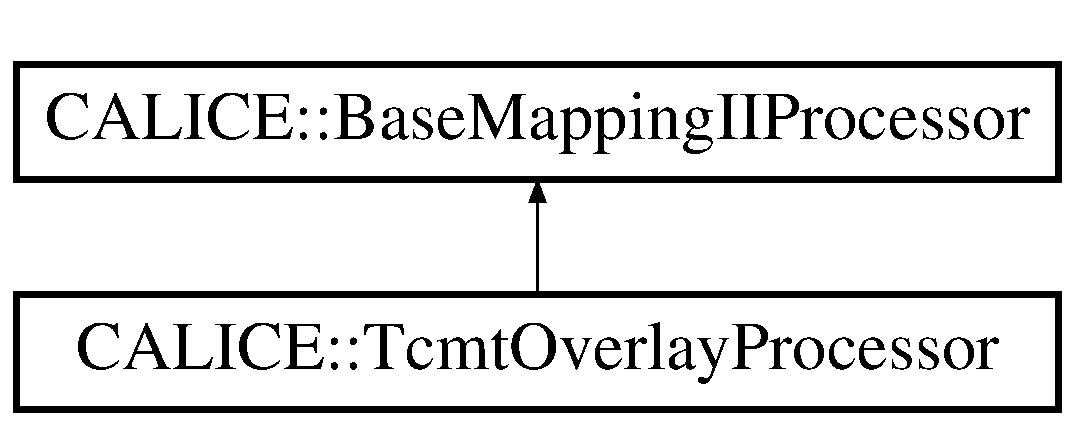
\includegraphics[height=2cm]{classCALICE_1_1TcmtOverlayProcessor}
\end{center}
\end{figure}
\subsection*{Public Member Functions}
\begin{DoxyCompactItemize}
\item 
{\bf TcmtOverlayProcessor} $\ast$ {\bfseries newProcessor} ()\label{classCALICE_1_1TcmtOverlayProcessor_a491ee74bd3a2849b4c5e590e78c5966e}

\item 
virtual void {\bfseries init} ()\label{classCALICE_1_1TcmtOverlayProcessor_a47c6fb10b94cdd75b6b2568f97163e57}

\item 
virtual void {\bfseries processEvent} (lcio::LCEvent $\ast$evt)\label{classCALICE_1_1TcmtOverlayProcessor_a19126164de84b0d41acf25e8d2074b93}

\item 
virtual void {\bfseries end} ()\label{classCALICE_1_1TcmtOverlayProcessor_a58abd4dd600627ba59982ad1458f795b}

\end{DoxyCompactItemize}
\subsection*{Protected Attributes}
\begin{DoxyCompactItemize}
\item 
std::string {\bfseries \_\-noiseColName}\label{classCALICE_1_1TcmtOverlayProcessor_ae5a9f82b50886731200994d68dd96909}

\item 
int {\bfseries \_\-noiseColType}\label{classCALICE_1_1TcmtOverlayProcessor_aa618736308ff49da01203210481bd9be}

\item 
float {\bfseries \_\-mipGev}\label{classCALICE_1_1TcmtOverlayProcessor_a9a4eb5151f1d1f92e91d40e6a3a1c4bb}

\item 
float {\bfseries \_\-energyThreshold}\label{classCALICE_1_1TcmtOverlayProcessor_ad34887a6904dc0accc0b84c810a175d7}

\item 
float {\bfseries \_\-maxDiff}\label{classCALICE_1_1TcmtOverlayProcessor_a4f6d55ec0342e5cd5576f5ecbc8b905c}

\item 
int {\bfseries \_\-maxDiffEvt}\label{classCALICE_1_1TcmtOverlayProcessor_ae90c13dd293d0acecd224d9e65a5737d}

\end{DoxyCompactItemize}


\subsection{Detailed Description}


Definition at line 18 of file TcmtOverlayProcessor.hh.

The documentation for this class was generated from the following files:\begin{DoxyCompactItemize}
\item 
TcmtOverlayProcessor.hh\item 
TcmtOverlayProcessor.cc\end{DoxyCompactItemize}

\section{CALICE::TempModel Class Reference}
\label{classCALICE_1_1TempModel}\index{CALICE::TempModel@{CALICE::TempModel}}
Inheritance diagram for CALICE::TempModel::\begin{figure}[H]
\begin{center}
\leavevmode
\includegraphics[height=2cm]{classCALICE_1_1TempModel}
\end{center}
\end{figure}
\subsection*{Public Member Functions}
\begin{DoxyCompactItemize}
\item 
virtual float {\bfseries getTemp} (lcio::LCCollection $\ast$col, unsigned moduleID, unsigned CellKey)\label{classCALICE_1_1TempModel_ad1cc8ffc2484c36beed93c4191b8e7e6}

\item 
virtual float {\bfseries getTempError} (lcio::LCCollection $\ast$col, unsigned moduleID, unsigned CellKey)\label{classCALICE_1_1TempModel_a8fab6288f361da8d51cb2b045497dd56}

\end{DoxyCompactItemize}


\subsection{Detailed Description}


Definition at line 14 of file TempModel.hh.

The documentation for this class was generated from the following file:\begin{DoxyCompactItemize}
\item 
TempModel.hh\end{DoxyCompactItemize}

\section{TBTrack::TrackFinder Class Reference}
\label{classTBTrack_1_1TrackFinder}\index{TBTrack::TrackFinder@{TBTrack::TrackFinder}}
\subsection*{Public Member Functions}
\begin{DoxyCompactItemize}
\item 
void {\bfseries alnConstants} (const {\bf AlnConstants} \&a)\label{classTBTrack_1_1TrackFinder_a6cb7c604ec9cf38348f22d050cc7bb49}

\item 
void {\bfseries fitConstants} (const {\bf FitConstants} \&p)\label{classTBTrack_1_1TrackFinder_aa1c57148ca9c5c72afb5045fcd2b55d3}

\item 
std::vector$<$ {\bf TrackProjection} $>$ {\bfseries find} (unsigned fb, unsigned eh, unsigned xy, const std::vector$<$ int $>$ \&v0, const std::vector$<$ int $>$ \&v1, const std::vector$<$ int $>$ \&v2, const std::vector$<$ int $>$ \&v3)\label{classTBTrack_1_1TrackFinder_a6378897788259d0afcd9cf9e40761bba}

\item 
std::ostream \& {\bfseries print} (std::ostream \&o) const \label{classTBTrack_1_1TrackFinder_a0b01ceac7e2eef542eafa25d656ba1b4}

\end{DoxyCompactItemize}
\subsection*{Private Attributes}
\begin{DoxyCompactItemize}
\item 
double {\bfseries \_\-probabilityCut} [4]\label{classTBTrack_1_1TrackFinder_af4cc2dd72bf92295fbe97b2382b65e15}

\item 
{\bf AlnConstants} {\bfseries \_\-alignment}\label{classTBTrack_1_1TrackFinder_ab100899aad4b03c3844f0e662d3fa86a}

\item 
{\bf TrackFitter} {\bfseries \_\-fitter} [2][2][2]\label{classTBTrack_1_1TrackFinder_a6e2c245adc3633995c352d177de4367d}

\end{DoxyCompactItemize}


\subsection{Detailed Description}


Definition at line 15 of file TrackFinder.hh.

The documentation for this class was generated from the following files:\begin{DoxyCompactItemize}
\item 
TrackFinder.hh\item 
TrackFinder.cc\end{DoxyCompactItemize}

\section{TBTrack::TrackFitInitialisation Class Reference}
\label{classTBTrack_1_1TrackFitInitialisation}\index{TBTrack::TrackFitInitialisation@{TBTrack::TrackFitInitialisation}}
\subsection*{Public Member Functions}
\begin{DoxyCompactItemize}
\item 
double {\bfseries zLayer} (unsigned l) const \label{classTBTrack_1_1TrackFitInitialisation_a01665c12db631dd5eceddd77bfe937e6}

\item 
void {\bfseries zLayer} (unsigned l, double z)\label{classTBTrack_1_1TrackFitInitialisation_afc1e65452855b3cd19aa5acb48e864f9}

\item 
double {\bfseries zBeam} () const \label{classTBTrack_1_1TrackFitInitialisation_a6bc7c5714057b2e01c19af17c1796ba2}

\item 
void {\bfseries zBeam} (double z)\label{classTBTrack_1_1TrackFitInitialisation_ae22fc580faa11890119c02707405bd07}

\item 
double {\bfseries beamCoordinate} () const \label{classTBTrack_1_1TrackFitInitialisation_a05f677ed046915cf6f8b82a854af182f}

\item 
double {\bfseries beamTanAngle} () const \label{classTBTrack_1_1TrackFitInitialisation_a7524b68beb3cacf9b185ae4ea7e1a81d}

\item 
void {\bfseries beamAverage} (double c, double t)\label{classTBTrack_1_1TrackFitInitialisation_a85507e913f3ff19274ad60673de58bdd}

\item 
const TMatrixDSym \& {\bfseries errorMatrix} () const \label{classTBTrack_1_1TrackFitInitialisation_ac7b30c88b39f27e822c33ea02876cfbb}

\item 
void {\bfseries errorMatrix} (const TMatrixDSym \&e)\label{classTBTrack_1_1TrackFitInitialisation_a12579080a3daa8d4dd257f7cf06e0754}

\item 
std::ostream \& {\bfseries print} (std::ostream \&o=std::cout, const std::string \&s=\char`\"{}\char`\"{}) const \label{classTBTrack_1_1TrackFitInitialisation_a3e2634a59a5ed407409f708755abdcea}

\end{DoxyCompactItemize}
\subsection*{Private Attributes}
\begin{DoxyCompactItemize}
\item 
double {\bfseries \_\-zLayer} [4]\label{classTBTrack_1_1TrackFitInitialisation_a6511a2ca609053513dccf4fff7900382}

\item 
double {\bfseries \_\-zBeam}\label{classTBTrack_1_1TrackFitInitialisation_aa15b79ff7fdac5ab332807bacde256e6}

\item 
double {\bfseries \_\-beamAverage} [2]\label{classTBTrack_1_1TrackFitInitialisation_a1fae67345661eeda08ad32937ae17e67}

\item 
TMatrixDSym {\bfseries \_\-errorMatrix}\label{classTBTrack_1_1TrackFitInitialisation_aa5d51d04eccb5d362c70d9bd2e51f765}

\end{DoxyCompactItemize}


\subsection{Detailed Description}


Definition at line 12 of file TrackFitInitialisation.hh.

The documentation for this class was generated from the following files:\begin{DoxyCompactItemize}
\item 
TrackFitInitialisation.hh\item 
TrackFitInitialisation.cc\end{DoxyCompactItemize}

\section{TBTrack::TrackFitResult Class Reference}
\label{classTBTrack_1_1TrackFitResult}\index{TBTrack::TrackFitResult@{TBTrack::TrackFitResult}}
Inheritance diagram for TBTrack::TrackFitResult::\begin{figure}[H]
\begin{center}
\leavevmode
\includegraphics[height=2cm]{classTBTrack_1_1TrackFitResult}
\end{center}
\end{figure}
\subsection*{Public Types}
\begin{DoxyCompactItemize}
\item 
enum \{ {\bfseries numberOfInts} = 0
 \}
\item 
enum \{ {\bfseries numberOfFloats} = 0
 \}
\item 
enum \{ {\bfseries numberOfDoubles} = 6
 \}
\end{DoxyCompactItemize}
\subsection*{Public Member Functions}
\begin{DoxyCompactItemize}
\item 
{\bfseries TrackFitResult} (double p0, double p1, const TMatrixDSym \&e, double c, unsigned h)\label{classTBTrack_1_1TrackFitResult_a9be66e8f2f6a85ee13202b35b3e49698}

\item 
void {\bfseries parameters} (double p0, double p1)\label{classTBTrack_1_1TrackFitResult_ad13aa283509c0e7ddca6815ef7a1cc57}

\item 
double {\bfseries intercept} (double z=0.0, double a=0.0) const \label{classTBTrack_1_1TrackFitResult_a7fbbf8ae46fa2ede02b6e9993608bf00}

\item 
double {\bfseries gradient} (double a=0.0) const \label{classTBTrack_1_1TrackFitResult_a4a5441700a888610c735ee01fd13e6d9}

\item 
TMatrixDSym {\bfseries errorMatrix} (double z=0.0, double a=0.0) const \label{classTBTrack_1_1TrackFitResult_a2c0e2dafabfbc64f26dd27497ea2fd75}

\item 
void {\bfseries errorMatrix} (const TMatrixDSym \&e)\label{classTBTrack_1_1TrackFitResult_ae70ea377e10c83a093cfc33680958f14}

\item 
double {\bfseries interceptError} (double z=0.0, double a=0.0) const \label{classTBTrack_1_1TrackFitResult_ae6cb4a2bba4e7f0e3fd18a764b7af88f}

\item 
double {\bfseries gradientError} (double a=0.0) const \label{classTBTrack_1_1TrackFitResult_a41f9c1f909254c6f08c2e755b15fd0c1}

\item 
double {\bfseries chiSquared} () const \label{classTBTrack_1_1TrackFitResult_a6e664b5e02b50c77e7036d0f500f8b86}

\item 
void {\bfseries chiSquared} (double c)\label{classTBTrack_1_1TrackFitResult_a6be030fd4473e6b5f1c49d3818e3449b}

\item 
int {\bfseries numberOfDof} () const \label{classTBTrack_1_1TrackFitResult_a1384e826d2e5e24b8edd6cf5ae3350d9}

\item 
double {\bfseries probability} () const \label{classTBTrack_1_1TrackFitResult_aba9d5aa99ef6d3c0c7c767f63e21191a}

\item 
unsigned {\bfseries hitPattern} () const \label{classTBTrack_1_1TrackFitResult_ad1988c2b480b8d45d9b92e6643a8f2b9}

\item 
void {\bfseries hitPattern} (unsigned h)\label{classTBTrack_1_1TrackFitResult_ac5b77c597472fbcf86b440940dbffc75}

\item 
unsigned {\bfseries numberOfHits} () const \label{classTBTrack_1_1TrackFitResult_a1911052615673f6341b65b4e874a7725}

\item 
std::ostream \& {\bfseries print} (std::ostream \&o=std::cout, const std::string \&s=\char`\"{}\char`\"{}) const \label{classTBTrack_1_1TrackFitResult_af6cc54a8c28eed7faf1a25680619c74e}

\item 
const int $\ast$ {\bfseries intData} () const \label{classTBTrack_1_1TrackFitResult_ad008025d62102edd1b766bcda8fca9d8}

\item 
int $\ast$ {\bfseries intData} ()\label{classTBTrack_1_1TrackFitResult_a9f6a52850d0d7fccf2fa679fefb156f9}

\item 
const float $\ast$ {\bfseries floatData} () const \label{classTBTrack_1_1TrackFitResult_af915d2a26e54410317c50e52072352a4}

\item 
float $\ast$ {\bfseries floatData} ()\label{classTBTrack_1_1TrackFitResult_acb8d400156d3413b0e1062530b87ecc9}

\item 
const double $\ast$ {\bfseries doubleData} () const \label{classTBTrack_1_1TrackFitResult_a91f32c7b577a192a2a97e645fec1c83c}

\item 
double $\ast$ {\bfseries doubleData} ()\label{classTBTrack_1_1TrackFitResult_a362625e95ba94f5de728a2cb3042c0cb}

\end{DoxyCompactItemize}
\subsection*{Protected Attributes}
\begin{DoxyCompactItemize}
\item 
double {\bfseries \_\-parameters} [2]\label{classTBTrack_1_1TrackFitResult_ae9b05a73283ac5d325e9bf1a07658854}

\item 
double {\bfseries \_\-errorMatrix} [3]\label{classTBTrack_1_1TrackFitResult_ac56f2127f056edc21a142686304b2acc}

\item 
double {\bfseries \_\-chiSquared}\label{classTBTrack_1_1TrackFitResult_acdb3c7423e9cb577feb311f30a8f31e7}

\item 
int {\bfseries \_\-hitPattern}\label{classTBTrack_1_1TrackFitResult_a585ab993aa74efcb9a0852df862d2be4}

\end{DoxyCompactItemize}


\subsection{Detailed Description}


Definition at line 12 of file TrackFitResult.hh.

The documentation for this class was generated from the following files:\begin{DoxyCompactItemize}
\item 
TrackFitResult.hh\item 
TrackFitResult.cc\end{DoxyCompactItemize}

\section{TBTrack::TrackFitter Class Reference}
\label{classTBTrack_1_1TrackFitter}\index{TBTrack::TrackFitter@{TBTrack::TrackFitter}}
\subsection*{Public Member Functions}
\begin{DoxyCompactItemize}
\item 
void {\bfseries fitInitialisation} (const {\bf TrackFitInitialisation} \&fc)\label{classTBTrack_1_1TrackFitter_a2460810173c203d8a9dab70f3481a48b}

\item 
{\bf TrackFitResult} {\bfseries fitResult} (unsigned h, const TVectorD \&c) const \label{classTBTrack_1_1TrackFitter_a1ecf97b17f92a8e151d751952a8a4077}

\item 
std::ostream \& {\bfseries print} (std::ostream \&o=std::cout, const std::string \&s=\char`\"{}\char`\"{}) const \label{classTBTrack_1_1TrackFitter_a8e2e95aaccd987917e16a9475e3ec37d}

\end{DoxyCompactItemize}
\subsection*{Private Attributes}
\begin{DoxyCompactItemize}
\item 
double {\bfseries \_\-beam} [2]\label{classTBTrack_1_1TrackFitter_a7863eee7e5607686b64eed9de3acc7ce}

\item 
{\bf LinearFitter} $\ast$ {\bfseries \_\-linearFitter} [64]\label{classTBTrack_1_1TrackFitter_a315a4d5931c5e1d1aea888f7d2b0679b}

\end{DoxyCompactItemize}


\subsection{Detailed Description}


Definition at line 17 of file TrackFitter.hh.

The documentation for this class was generated from the following files:\begin{DoxyCompactItemize}
\item 
TrackFitter.hh\item 
TrackFitter.cc\end{DoxyCompactItemize}

\section{TBTrack::TrackProjection Class Reference}
\label{classTBTrack_1_1TrackProjection}\index{TBTrack::TrackProjection@{TBTrack::TrackProjection}}
Inheritance diagram for TBTrack::TrackProjection::\begin{figure}[H]
\begin{center}
\leavevmode
\includegraphics[height=2cm]{classTBTrack_1_1TrackProjection}
\end{center}
\end{figure}
\subsection*{Public Member Functions}
\begin{DoxyCompactItemize}
\item 
{\bfseries TrackProjection} (const {\bf TBTrack::TrackFitResult} \&r)\label{classTBTrack_1_1TrackProjection_a5687005151617c3972c01967fe2da734}

\item 
{\bfseries TrackProjection} (const EVENT::LCGenericObject $\ast$p)\label{classTBTrack_1_1TrackProjection_a3113d8b470f7a8e4de211e43a7d50fd6}

\item 
unsigned {\bfseries xy} () const \label{classTBTrack_1_1TrackProjection_a9d48d08c834d07e778d4381fb974505b}

\item 
unsigned {\bfseries fb} () const \label{classTBTrack_1_1TrackProjection_ad24e264233b83d4c9cd813881f2fbac7}

\item 
unsigned {\bfseries eh} () const \label{classTBTrack_1_1TrackProjection_a44289793d84283f8ff664659fd25821e}

\item 
void {\bfseries fitType} (unsigned xy, unsigned fb, unsigned eh)\label{classTBTrack_1_1TrackProjection_ae0c43b50ae45c6e13c4bb01f09b3e74f}

\item 
void {\bfseries hit} (unsigned i, int t)\label{classTBTrack_1_1TrackProjection_ad2e6a1f8c2a971adf982d67b571f7292}

\item 
int {\bfseries hit} (unsigned i) const \label{classTBTrack_1_1TrackProjection_a3f563df4496127397acd6f047797ba0c}

\item 
void {\bfseries set} (const EVENT::LCGenericObject $\ast$p)\label{classTBTrack_1_1TrackProjection_ad31ce23afa4dd066bd49bc30ba7962fe}

\item 
EVENT::LCGenericObject $\ast$ {\bfseries get} () const \label{classTBTrack_1_1TrackProjection_abbf79bbd22e4f0c139277bb90ee4ccdd}

\item 
std::ostream \& {\bfseries print} (std::ostream \&o=std::cout, const std::string \&s=\char`\"{}\char`\"{}) const \label{classTBTrack_1_1TrackProjection_ab01859ecafcdf84813fa159a9a716d4d}

\end{DoxyCompactItemize}
\subsection*{Private Attributes}
\begin{DoxyCompactItemize}
\item 
int {\bfseries \_\-fitType}\label{classTBTrack_1_1TrackProjection_ac62ce7e8caa0726293c426b63be9afb0}

\item 
int {\bfseries \_\-hits} [4]\label{classTBTrack_1_1TrackProjection_a68bc579b0e61af75267ac3cc3fa72663}

\end{DoxyCompactItemize}


\subsection{Detailed Description}


Definition at line 18 of file TrackProjection.hh.

The documentation for this class was generated from the following files:\begin{DoxyCompactItemize}
\item 
TrackProjection.hh\item 
TrackProjection.cc\end{DoxyCompactItemize}

\section{CALICE::TriggerAnalysis Class Reference}
\label{classCALICE_1_1TriggerAnalysis}\index{CALICE::TriggerAnalysis@{CALICE::TriggerAnalysis}}


Search for good trigger words.  


{\ttfamily \#include $<$TriggerAnalysis.hh$>$}\subsection*{Public Member Functions}
\begin{DoxyCompactItemize}
\item 
Processor $\ast$ {\bfseries newProcessor} ()\label{classCALICE_1_1TriggerAnalysis_ab21f54611eb9ddd3ad43fc21503d4e33}

\item 
void {\bf init} ()\label{classCALICE_1_1TriggerAnalysis_a7a51af68dccbac1354f5246cdcea5c83}

\begin{DoxyCompactList}\small\item\em Set up conditions data handler, verify parameters et.c. \item\end{DoxyCompactList}\item 
void {\bf processEvent} (LCEvent $\ast$evtP)
\begin{DoxyCompactList}\small\item\em Called for every run (does nothing. \item\end{DoxyCompactList}\item 
void {\bfseries end} ()\label{classCALICE_1_1TriggerAnalysis_a3dc3f0ae7a921facafc54fa4e271f664}

\end{DoxyCompactItemize}
\subsection*{Private Attributes}
\begin{DoxyCompactItemize}
\item 
std::string {\bf \_\-parNameTriggerMainWord}
\begin{DoxyCompactList}\small\item\em Par. \item\end{DoxyCompactList}\item 
unsigned int {\bfseries \_\-nEvents}\label{classCALICE_1_1TriggerAnalysis_ad08524b6d02fb2d7b75b172652b1d435}

\item 
unsigned int {\bfseries \_\-missingTriggerEventData}\label{classCALICE_1_1TriggerAnalysis_aee5bbae4a0166c2432de8eaa16fa6dca}

\item 
{\bf histmgr::Key\_\-t} {\bf \_\-histGroupKey}
\begin{DoxyCompactList}\small\item\em Key for the histogram group. \item\end{DoxyCompactList}\item 
{\bf histmgr::Key\_\-t} {\bf \_\-histTriggerOnPosisitonKey}
\begin{DoxyCompactList}\small\item\em Key for the trigger on position histograms. \item\end{DoxyCompactList}\item 
{\bf histmgr::Key\_\-t} {\bf \_\-histTriggerLengthKey}
\begin{DoxyCompactList}\small\item\em Key for the trigger pulse length histograms. \item\end{DoxyCompactList}\end{DoxyCompactItemize}


\subsection{Detailed Description}
Search for good trigger words. 

Definition at line 22 of file TriggerAnalysis.hh.

\subsection{Member Function Documentation}
\index{CALICE::TriggerAnalysis@{CALICE::TriggerAnalysis}!processEvent@{processEvent}}
\index{processEvent@{processEvent}!CALICE::TriggerAnalysis@{CALICE::TriggerAnalysis}}
\subsubsection[{processEvent}]{\setlength{\rightskip}{0pt plus 5cm}void CALICE::TriggerAnalysis::processEvent (LCEvent $\ast$ {\em evtP})}\label{classCALICE_1_1TriggerAnalysis_a687740dc2b5d83e9bbcd705dede331ef}


Called for every run (does nothing. ) Search good trigger words. If no good trigger word is found a damaged flag is set in the event header. 

Definition at line 135 of file TriggerAnalysis.cc.

References \_\-histGroupKey, \_\-histTriggerLengthKey, \_\-histTriggerOnPosisitonKey, \_\-parNameTriggerMainWord, histmgr::HistMgr::getHistogramCollection(), and histmgr::HistogramCollection\_\-t::histogram().

\subsection{Field Documentation}
\index{CALICE::TriggerAnalysis@{CALICE::TriggerAnalysis}!\_\-histGroupKey@{\_\-histGroupKey}}
\index{\_\-histGroupKey@{\_\-histGroupKey}!CALICE::TriggerAnalysis@{CALICE::TriggerAnalysis}}
\subsubsection[{\_\-histGroupKey}]{\setlength{\rightskip}{0pt plus 5cm}{\bf histmgr::Key\_\-t} {\bf CALICE::TriggerAnalysis::\_\-histGroupKey}\hspace{0.3cm}{\ttfamily  [private]}}\label{classCALICE_1_1TriggerAnalysis_ac6c3ea8f3ff2b56e809f4969f59704d3}


Key for the histogram group. 

Definition at line 58 of file TriggerAnalysis.hh.

Referenced by init(), and processEvent().\index{CALICE::TriggerAnalysis@{CALICE::TriggerAnalysis}!\_\-histTriggerLengthKey@{\_\-histTriggerLengthKey}}
\index{\_\-histTriggerLengthKey@{\_\-histTriggerLengthKey}!CALICE::TriggerAnalysis@{CALICE::TriggerAnalysis}}
\subsubsection[{\_\-histTriggerLengthKey}]{\setlength{\rightskip}{0pt plus 5cm}{\bf histmgr::Key\_\-t} {\bf CALICE::TriggerAnalysis::\_\-histTriggerLengthKey}\hspace{0.3cm}{\ttfamily  [private]}}\label{classCALICE_1_1TriggerAnalysis_a4af95b807dcdd3389a2b64663f31e6db}


Key for the trigger pulse length histograms. 

Definition at line 60 of file TriggerAnalysis.hh.

Referenced by init(), and processEvent().\index{CALICE::TriggerAnalysis@{CALICE::TriggerAnalysis}!\_\-histTriggerOnPosisitonKey@{\_\-histTriggerOnPosisitonKey}}
\index{\_\-histTriggerOnPosisitonKey@{\_\-histTriggerOnPosisitonKey}!CALICE::TriggerAnalysis@{CALICE::TriggerAnalysis}}
\subsubsection[{\_\-histTriggerOnPosisitonKey}]{\setlength{\rightskip}{0pt plus 5cm}{\bf histmgr::Key\_\-t} {\bf CALICE::TriggerAnalysis::\_\-histTriggerOnPosisitonKey}\hspace{0.3cm}{\ttfamily  [private]}}\label{classCALICE_1_1TriggerAnalysis_a9e02480c102f82efe0629255b7bc1bd3}


Key for the trigger on position histograms. 

Definition at line 59 of file TriggerAnalysis.hh.

Referenced by init(), and processEvent().\index{CALICE::TriggerAnalysis@{CALICE::TriggerAnalysis}!\_\-parNameTriggerMainWord@{\_\-parNameTriggerMainWord}}
\index{\_\-parNameTriggerMainWord@{\_\-parNameTriggerMainWord}!CALICE::TriggerAnalysis@{CALICE::TriggerAnalysis}}
\subsubsection[{\_\-parNameTriggerMainWord}]{\setlength{\rightskip}{0pt plus 5cm}std::string {\bf CALICE::TriggerAnalysis::\_\-parNameTriggerMainWord}\hspace{0.3cm}{\ttfamily  [private]}}\label{classCALICE_1_1TriggerAnalysis_a4601167e6fe8aa42e2336a893bf83a21}


Par. name of the trigger main word. 

Definition at line 53 of file TriggerAnalysis.hh.

Referenced by processEvent().

The documentation for this class was generated from the following files:\begin{DoxyCompactItemize}
\item 
TriggerAnalysis.hh\item 
TriggerAnalysis.cc\end{DoxyCompactItemize}

\section{vector Class Reference}
\label{classstd_1_1vector}\index{std::vector@{std::vector}}


Inherited by {\bf SimpleArray\_\-t$<$ CellIndexArray\_\-t $>$}, {\bf SimpleArray\_\-t$<$ ModuleConnection $>$}, {\bf SimpleArray\_\-t$<$ ModuleDescription $>$}, {\bf SimpleArray\_\-t$<$ pair$<$ UInt\_\-t, ModuleLocation $>$ $>$}, and {\bf SimpleArray\_\-t$<$ pair$<$ UInt\_\-t, SlotList\_\-t $>$ $>$}.

The documentation for this class was generated from the following file:\begin{DoxyCompactItemize}
\item 
SimpleArray\_\-t.hh\end{DoxyCompactItemize}

\section{CALICE::VRawADCValueProcessor Class Reference}
\label{classCALICE_1_1VRawADCValueProcessor}\index{CALICE::VRawADCValueProcessor@{CALICE::VRawADCValueProcessor}}


Abstract class which implements the minimal functionality to access raw ADC values.  


{\ttfamily \#include $<$VRawADCValueProcessor.hh$>$}Inheritance diagram for CALICE::VRawADCValueProcessor::\begin{figure}[H]
\begin{center}
\leavevmode
\includegraphics[height=0.683761cm]{classCALICE_1_1VRawADCValueProcessor}
\end{center}
\end{figure}
\subsection*{Protected Member Functions}
\begin{DoxyCompactItemize}
\item 
{\bfseries VRawADCValueProcessor} (const std::string \&processor\_\-name)\label{classCALICE_1_1VRawADCValueProcessor_aaf1fa3484d50b2a28f96f3ec3853e9cc}

\item 
void {\bfseries init} ()\label{classCALICE_1_1VRawADCValueProcessor_a68246236e2ed3c612b9617234655d2a1}

\item 
virtual void {\bfseries moduleTypeChanged} (lcio::LCCollection $\ast$col)\label{classCALICE_1_1VRawADCValueProcessor_a40c7f7d113fff799c0334c7b773b5513}

\item 
virtual void {\bfseries moduleLocationChanged} (lcio::LCCollection $\ast$col)\label{classCALICE_1_1VRawADCValueProcessor_a11391eed95cf78c653dca943c1444134}

\item 
virtual void {\bfseries stagePositionChanged} (lcio::LCCollection $\ast$col)\label{classCALICE_1_1VRawADCValueProcessor_ac1206e19dae92b34ee26dcbee542c3ab}

\item 
virtual void {\bfseries moduleConnectionChanged} (lcio::LCCollection $\ast$col)\label{classCALICE_1_1VRawADCValueProcessor_af79356a56727b21864897f799b2e98ed}

\item 
void {\bfseries showCollectionParameters} (LCCollection $\ast$colP)\label{classCALICE_1_1VRawADCValueProcessor_a5cd308af8668b39a2dc93eafc1fba03c}

\item 
void {\bfseries correctModuleDescriptionOrder} (LCCollection $\ast$colP)\label{classCALICE_1_1VRawADCValueProcessor_a3f3ae1c5de99f40e5682aa35200d0365}

\end{DoxyCompactItemize}
\subsection*{Protected Attributes}
\begin{DoxyCompactItemize}
\item 
MappingAndAlignment {\bfseries \_\-mapping}\label{classCALICE_1_1VRawADCValueProcessor_a04dcae798efd66211f1fe66686e2fb60}

\item 
std::string {\bf \_\-adcColName}
\begin{DoxyCompactList}\small\item\em Name of the input collection (INPUT). \item\end{DoxyCompactList}\item 
std::string {\bf \_\-colNameModuleDescription}
\begin{DoxyCompactList}\small\item\em Name of the conditions data collection containing module descriptions. \item\end{DoxyCompactList}\item 
std::string {\bf \_\-colNameModuleLocation}
\begin{DoxyCompactList}\small\item\em Name of the conditions data collection containing module location. \item\end{DoxyCompactList}\item 
std::string {\bf \_\-colNameModuleConnection}
\begin{DoxyCompactList}\small\item\em Name of the conditions data collection containing module location. \item\end{DoxyCompactList}\item 
std::string {\bf \_\-colNameStageCollection}
\begin{DoxyCompactList}\small\item\em Name of the conditions data collection containing stage positions. \item\end{DoxyCompactList}\item 
ConditionsChangeDelegator$<$ {\bf VRawADCValueProcessor} $>$ {\bf \_\-moduleTypeChange}\label{classCALICE_1_1VRawADCValueProcessor_af8af90b149e3fe18b894756535eb2cfe}

\begin{DoxyCompactList}\small\item\em helper class to listen for changes of the module types (conditions data) \item\end{DoxyCompactList}\item 
ConditionsChangeDelegator$<$ {\bf VRawADCValueProcessor} $>$ {\bf \_\-moduleLocationChange}\label{classCALICE_1_1VRawADCValueProcessor_af8355db99526cb3be8df7d5b0057a1ea}

\begin{DoxyCompactList}\small\item\em helper class to listen for changes of the location of modules (conditions data) \item\end{DoxyCompactList}\item 
ConditionsChangeDelegator$<$ {\bf VRawADCValueProcessor} $>$ {\bf \_\-moduleConnectionChange}\label{classCALICE_1_1VRawADCValueProcessor_a854695da8e7fe2c647ac8415367987d5}

\begin{DoxyCompactList}\small\item\em helper class to listen for changes of the connection between modules and the DAQ front-\/ends (conditions data) \item\end{DoxyCompactList}\item 
ConditionsChangeDelegator$<$ {\bf VRawADCValueProcessor} $>$ {\bf \_\-stagePositionChange}\label{classCALICE_1_1VRawADCValueProcessor_a9aec2fb84d7a380d73995bf3d21205b9}

\begin{DoxyCompactList}\small\item\em helper class to listen for changes of stage positions (conditions data) \item\end{DoxyCompactList}\item 
unsigned int {\bfseries \_\-wrongOrderTill}\label{classCALICE_1_1VRawADCValueProcessor_ac89301a31fbc0418b25ebd3c7c3680f9}

\end{DoxyCompactItemize}


\subsection{Detailed Description}
Abstract class which implements the minimal functionality to access raw ADC values. 

Definition at line 18 of file VRawADCValueProcessor.hh.

\subsection{Field Documentation}
\index{CALICE::VRawADCValueProcessor@{CALICE::VRawADCValueProcessor}!\_\-adcColName@{\_\-adcColName}}
\index{\_\-adcColName@{\_\-adcColName}!CALICE::VRawADCValueProcessor@{CALICE::VRawADCValueProcessor}}
\subsubsection[{\_\-adcColName}]{\setlength{\rightskip}{0pt plus 5cm}std::string {\bf CALICE::VRawADCValueProcessor::\_\-adcColName}\hspace{0.3cm}{\ttfamily  [protected]}}\label{classCALICE_1_1VRawADCValueProcessor_a9af055c07a4e40284ba7851ee901d7af}


Name of the input collection (INPUT). 

Definition at line 28 of file VRawADCValueProcessor.hh.

Referenced by CALICE::SimpleHitSearch::accumulateEventsForInitialPedestalNoiseCalculation(), CALICE::SimpleHitSearch::accumulateEventsForPedestalNoiseCalculationWithHitRejection(), CALICE::SimpleHitSearch::accumulateEventsForPedestalNoiseCalculationWithHitRejectionAndPedestalShiftDetection(), CALICE::AverageHistoryGraphs::processEvent(), CALICE::SimpleHitSearch::searchHits(), and CALICE::SimpleHitSearch::searchHitsAndAdjustPedestalsAndNoise().\index{CALICE::VRawADCValueProcessor@{CALICE::VRawADCValueProcessor}!\_\-colNameModuleConnection@{\_\-colNameModuleConnection}}
\index{\_\-colNameModuleConnection@{\_\-colNameModuleConnection}!CALICE::VRawADCValueProcessor@{CALICE::VRawADCValueProcessor}}
\subsubsection[{\_\-colNameModuleConnection}]{\setlength{\rightskip}{0pt plus 5cm}std::string {\bf CALICE::VRawADCValueProcessor::\_\-colNameModuleConnection}\hspace{0.3cm}{\ttfamily  [protected]}}\label{classCALICE_1_1VRawADCValueProcessor_a186586ecdee3ab773bdd40ad3e8594dc}


Name of the conditions data collection containing module location. 

Definition at line 33 of file VRawADCValueProcessor.hh.\index{CALICE::VRawADCValueProcessor@{CALICE::VRawADCValueProcessor}!\_\-colNameModuleDescription@{\_\-colNameModuleDescription}}
\index{\_\-colNameModuleDescription@{\_\-colNameModuleDescription}!CALICE::VRawADCValueProcessor@{CALICE::VRawADCValueProcessor}}
\subsubsection[{\_\-colNameModuleDescription}]{\setlength{\rightskip}{0pt plus 5cm}std::string {\bf CALICE::VRawADCValueProcessor::\_\-colNameModuleDescription}\hspace{0.3cm}{\ttfamily  [protected]}}\label{classCALICE_1_1VRawADCValueProcessor_a7c7446a4e691d62dbeaaf09d64122af0}


Name of the conditions data collection containing module descriptions. 

Definition at line 31 of file VRawADCValueProcessor.hh.

Referenced by CALICE::SimpleHitSearch::init(), and CALICE::CalibrateAndApplyThreshold::init().\index{CALICE::VRawADCValueProcessor@{CALICE::VRawADCValueProcessor}!\_\-colNameModuleLocation@{\_\-colNameModuleLocation}}
\index{\_\-colNameModuleLocation@{\_\-colNameModuleLocation}!CALICE::VRawADCValueProcessor@{CALICE::VRawADCValueProcessor}}
\subsubsection[{\_\-colNameModuleLocation}]{\setlength{\rightskip}{0pt plus 5cm}std::string {\bf CALICE::VRawADCValueProcessor::\_\-colNameModuleLocation}\hspace{0.3cm}{\ttfamily  [protected]}}\label{classCALICE_1_1VRawADCValueProcessor_a3b5a772ddae19bfabcaff86428defd1c}


Name of the conditions data collection containing module location. 

Definition at line 32 of file VRawADCValueProcessor.hh.\index{CALICE::VRawADCValueProcessor@{CALICE::VRawADCValueProcessor}!\_\-colNameStageCollection@{\_\-colNameStageCollection}}
\index{\_\-colNameStageCollection@{\_\-colNameStageCollection}!CALICE::VRawADCValueProcessor@{CALICE::VRawADCValueProcessor}}
\subsubsection[{\_\-colNameStageCollection}]{\setlength{\rightskip}{0pt plus 5cm}std::string {\bf CALICE::VRawADCValueProcessor::\_\-colNameStageCollection}\hspace{0.3cm}{\ttfamily  [protected]}}\label{classCALICE_1_1VRawADCValueProcessor_a4af3c2f4f81070c495ea68090acb6386}


Name of the conditions data collection containing stage positions. 

Definition at line 34 of file VRawADCValueProcessor.hh.

The documentation for this class was generated from the following files:\begin{DoxyCompactItemize}
\item 
VRawADCValueProcessor.hh\item 
VRawADCValueProcessor.cc\end{DoxyCompactItemize}

\section{CALICE::WaferInfo\_\-t Class Reference}
\label{classCALICE_1_1WaferInfo__t}\index{CALICE::WaferInfo\_\-t@{CALICE::WaferInfo\_\-t}}
\subsection*{Public Member Functions}
\begin{DoxyCompactItemize}
\item 
void {\bfseries addBorderHit} ()\label{classCALICE_1_1WaferInfo__t_a667fa0a1634c214a3a6a98b6ce85ea68}

\item 
void {\bfseries addInnerHit} ()\label{classCALICE_1_1WaferInfo__t_afe1f12f38383236ddbb28ca6ee269c77}

\item 
void {\bfseries addHitSignal} (Float\_\-t energy, unsigned char col\_\-i, unsigned char row\_\-i)\label{classCALICE_1_1WaferInfo__t_a21e55668bddc8d4cc6b1814b9bbad307}

\item 
unsigned char {\bfseries nBorderHits} () const \label{classCALICE_1_1WaferInfo__t_a06d289e3d9c3b3d5a348b5a7f994d019}

\item 
unsigned char {\bfseries nInnerHits} () const \label{classCALICE_1_1WaferInfo__t_af7305039ddf2ea5cf7f97a9dcba2c276}

\item 
unsigned char {\bfseries maxRow} () const \label{classCALICE_1_1WaferInfo__t_a308f72e84cbefc4ac5694b2049969cef}

\item 
unsigned char {\bfseries maxCol} () const \label{classCALICE_1_1WaferInfo__t_ac7a95b41317f75a0fa1b97a6a909d294}

\item 
Float\_\-t {\bfseries maxSignal} () const \label{classCALICE_1_1WaferInfo__t_a19ddba62ea3924e9eb140838fc532882}

\item 
Float\_\-t {\bfseries totalSignal} () const \label{classCALICE_1_1WaferInfo__t_a59ad431cbb3005e069ee137988a034b1}

\end{DoxyCompactItemize}
\subsection*{Data Fields}
\begin{DoxyCompactItemize}
\item 
unsigned char {\bfseries \_\-nBorderHits}\label{classCALICE_1_1WaferInfo__t_a621edca54c4166f865da90aa8b395ea7}

\item 
unsigned char {\bfseries \_\-nInnerHits}\label{classCALICE_1_1WaferInfo__t_a00278142ce3014e3c2f7d98202adcf80}

\item 
unsigned char {\bfseries \_\-maxRow}\label{classCALICE_1_1WaferInfo__t_a41c81c4926b86743f170e8faeadff528}

\item 
unsigned char {\bfseries \_\-maxCol}\label{classCALICE_1_1WaferInfo__t_a92af46b078ed24127a392ffe7aa27b05}

\item 
Float\_\-t {\bfseries \_\-maxSignal}\label{classCALICE_1_1WaferInfo__t_ac2a779dbfcccd850562e96b2fc397014}

\item 
Float\_\-t {\bfseries \_\-totalSignal}\label{classCALICE_1_1WaferInfo__t_ac0f78a4c015765f1d71de3d2a55d1ef0}

\end{DoxyCompactItemize}


\subsection{Detailed Description}


Definition at line 169 of file SquareFinder.cc.

The documentation for this class was generated from the following file:\begin{DoxyCompactItemize}
\item 
SquareFinder.cc\end{DoxyCompactItemize}

\printindex
\end{document}
